\changefontsizes{20pt}
\chapter{Feedback with Feedforward Control (Pre-control)}
\label{cha:chap5}
\changefontsizes{12pt}
For pre-control, the net imbalance forces and torques are fed forward to the controller along with the feedback position control. The control system is illustrated in Figure \ref{fig:precontrol}. Thus, the controller effort $\mathbf{u}$ is a function of both the deviation of the bike centre of gravity from the reference position, and the net imbalances on the bike ($\mathbf{d}$).

\begin{figure}[h!]
	\centering
	\tikzstyle{block}     = [draw, rectangle, minimum height=1.5cm, minimum width=1.6cm]
	\tikzstyle{branch}    = [circle, inner sep=0pt, minimum size=0.01mm, fill=black, draw=black]
	\tikzstyle{connector} = [->, thick]
	\tikzstyle{dummy}     = [inner sep=0pt, minimum size=0pt]
	\tikzstyle{inout}     = []
	\tikzstyle{sum}       = [circle, inner sep=0pt, minimum size=2mm, draw=black, thick]
	\begin{tikzpicture}[auto, node distance=3cm, >=stealth']
		\node[block] (bike) {CF};
		\node[block, left of = bike, node distance = 7cm] (PD) {$\begin{matrix}
				K_x&&\\
				&K_y&\\
				&&K_z
			\end{matrix}$};
		\node[inout, above of = bike,node distance = 2cm] (d) {\textbf{d}};
		\node[block, left of = d] (precontrol) {$\mathbf{K}_d$};
		\node[inout,right of = bike] (y) {\textbf{y}};
		\node[sum,left of = PD,node distance = 2cm] (s) {};
		\node[sum,left of = bike] (s1) {};
		\node[branch,right of = bike,node distance = 1.5cm] (b1) {};
		\node[branch,below of = b1] (b2) {};
		
		\draw[connector] (bike) -- (y);
		\draw[thick] (b1) -- (b2);
		\draw[connector] (b2) -| (s);
		\draw[connector] (s) -- (PD);
		\draw[connector] (d) -- (precontrol);
		\draw[connector] (precontrol) -- (s1);
		\draw[connector] (PD) -- (s1);
		\draw[connector] (s1) -- node{\textbf{u}} (bike);
		
	\end{tikzpicture}
	\caption{Pre-Control}
	\label{fig:precontrol}
\end{figure}

% --------------------------------------------------------------------------
% 		Section 5.1
% --------------------------------------------------------------------------

\section{Motivation}
The idea behind the use of pre-control is the anticipation of the imbalance in the excitations which are fed to the CF Bike. The concept of imbalance anticipation is illustrated in Figure \ref{fig:precontrolMotivation}, where a set of hypothetical load plots for the handlebar and the rearhub for a small time frame $\Delta t$ is shown. In the CF Bike simulation, the bike will start its deviation from its position primarily because of the imbalance, specifically when the imbalance is large enough to translate/rotate the bike frame. Then based on the resultant deviation, the position control will react and try to regulate the bike. This reaction will not coincide with the time instant at which the imbalance first starts, since the imbalance will take some time to be large enough to create the position change of the bike. Such a point where the position control starts reacting is depicted as B and $t_B$ in the figure. When precontrol is used, we are directly feeding in the information about the imbalance to the controller, thus the controller will know the exact time at which the imbalance starts. The starting point of the imbalance is shown as A and $t_A$ in the figure. Thus, the controller will start reacting faster to compensate the imbalance and ideally it should lead to a better control performance of the CF Bike.

\begin{figure}[h!]
	\centering
	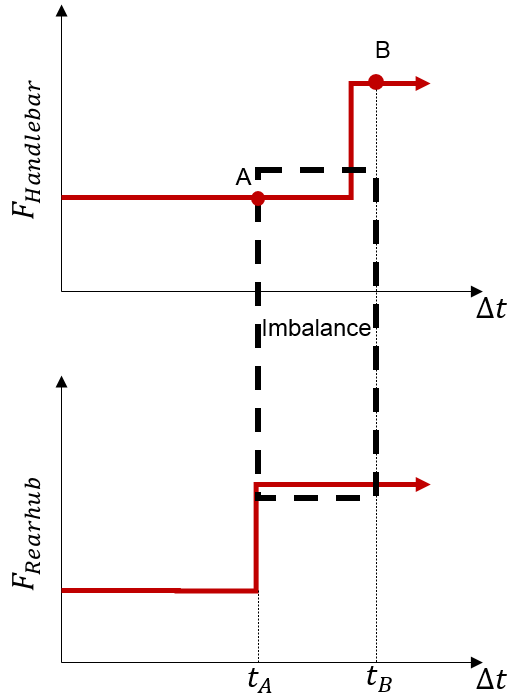
\includegraphics[scale = 0.45]{Contents/Resources/Precontrol/Motivation.png}
	\caption{Imbalance anticipation}
	\label{fig:precontrolMotivation}
\end{figure}

% --------------------------------------------------------------------------
% 		Section 5.2
% --------------------------------------------------------------------------

\section{Varying Pre-Control Gains}
The feedforward controller ($\mathbf{K}_d$) is considered to be decentralised like the feedback controller, and is considered to be constant. $$\mathbf{K}_d = \begin{bmatrix}
	k_1&0&0\\
	0&k_2&0\\
	0&0&k_3
\end{bmatrix}$$
Thus, the controller effort looks like:
\begin{align*}
	&u_x = K_x\Delta x + k_1d_x\\
	&u_y = K_y\Delta y + k_2d_y\\
	&u_z = K_z\Delta \gamma + k_3d_z
\end{align*}

The tabulated controller performance for $k_1 = k_2 = k_3 = 1$ and $k_1 = k_2 = k_3 = -1$ and PD Feedback Control are shown in tables \ref{tab:precontrolA1} to \ref{tab:precontrolC2}.

\begin{table}[h]
	\centering
	\begin{tabular}{ |c|c|c|c| } 
		\hline
		Forces & Mean Error (\%) & RMSE & $R_2$\\ 
		\hline
		FX & 3&128&0.98\\ 
		FY & 101&970&0.01 \\ 
		\hline
	\end{tabular}
	\caption{Load Errors at Point A of CF with PD Control and Pre-control with gains $\{-1,-1,-1\}$}
	\label{tab:precontrolA1}
\end{table}

\begin{table}[h]
	\centering
	\begin{tabular}{ |c|c|c|c| } 
		\hline
		Forces & Mean Error (\%) & RMSE & $R_2$\\ 
		\hline
		FX & 4&15&0.98\\ 
		FY & 4&2&0.98 \\ 
		\hline
	\end{tabular}
	\caption{Load Errors at Point B of CF with PD Control and Pre-control with gains $\{-1,-1,-1\}$}
	\label{tab:precontrolB1}
\end{table}

\begin{table}[h!]
	\centering
	\begin{tabular}{ |c|c|c|c| } 
		\hline
		Forces & Mean Error (\%) & RMSE & $R_2$\\ 
		\hline
		FX & 4&154&0.95\\ 
		FY & 59&972&0.05 \\ 
		\hline
	\end{tabular}
	\caption{Load Errors at Point C of CF with PD Control and Pre-control with gains $\{-1,-1,-1\}$}
	\label{tab:precontrolC1}
\end{table}

\begin{table}[h!]
	\centering
	\begin{tabular}{ |c|c|c|c| } 
		\hline
		Forces & Mean Error (\%) & RMSE & $R_2$\\ 
		\hline
		FX & 3&129&0.98\\ 
		FY & 103&914&0 \\ 
		\hline
	\end{tabular}
	\caption{Load Errors at Point A of CF with PD Control and Pre-control with gains $\{1,1,1\}$}
	\label{tab:precontrolA2}
\end{table}

\begin{table}[h!]
	\centering
	\begin{tabular}{ |c|c|c|c| } 
		\hline
		Forces & Mean Error (\%) & RMSE & $R_2$\\ 
		\hline
		FX & 4&16&0.98\\ 
		FY & 4&2&0.98 \\ 
		\hline
	\end{tabular}
	\caption{Load Errors at Point B of CF with PD Control and Pre-control with gains $\{1,1,1\}$}
	\label{tab:precontrolB2}
\end{table}

\begin{table}[h!]
	\centering
	\begin{tabular}{ |c|c|c|c| } 
		\hline
		Forces & Mean Error (\%) & RMSE & $R_2$\\ 
		\hline
		FX & 4&155&0.95\\ 
		FY & 59&912&0.03 \\ 
		\hline
	\end{tabular}
	\caption{Load Errors at Point C of CF with PD Control and Pre-control with gains $\{1,1,1\}$}
	\label{tab:precontrolC2}
\end{table}

It can be seen that irrespective of the feedforward gains, the results don't improve or degrade by a very significant margin. Infact, it was observed after multiple simulation runs of different feedforward gains combined with different feedback controllers that using pre-control doesn't have a very (positive or negative) significant effect on the performance that pure feedback control was showing. Thus, our hypothesis regarding the perceived benefit of pre-control is more or less proved wrong.

% --------------------------------------------------------------------------
% 		Section 5.3
% --------------------------------------------------------------------------

\section{Eliminating CF Angular Position Feedback}
\label{sec:noFeedback}
As mentioned in Chapter \ref{cha:chap3}, for almost all purely feedback controllers, the control torque ($u_z$) was always significantly less than the net imbalance torque experienced by the bike. This is also true when pre-control is used. The likely reason for this might be the compensation in position provided by the feedback of the rotation of the CF Bike. Thus, the feedback of the angular position of the CF Bike ($\gamma$) is eliminated along with PD Control of the X and Y positions of CF Bike along with pre-control still activated. In this case, we have to be cautious since about the Z axis, a feedforward torque is directly fed without feedback, and as observed in section \ref{sec:chap3sec2} of chapter \ref{cha:chap3}, directly feedforwarding forces or torques without feedback leads to instability of the CF Bike. Thus, the pre-control gain about the Z axis is kept very low. Tables \ref{tab:noZfdkA} to \ref{tab:noZfdkC} show the tabulated performance with no Z-feedback. 

\begin{table}[h!]
	\centering
	\begin{tabular}{ |c|c|c|c| } 
		\hline
		Forces & Mean Error (\%) & RMSE & $R_2$\\ 
		\hline
		FX & 15&324&0.95\\ 
		FY & 13&177&0.94 \\ 
		\hline
	\end{tabular}
	\caption{Load Errors at point A of CF with no Z Feedback and Pre-control with gains $\{0,0,-0.1\}$}
	\label{tab:noZfdkA}
\end{table}

\begin{table}[h!]
	\centering
	\begin{tabular}{ |c|c|c|c| } 
		\hline
		Forces & Mean Error (\%) & RMSE & $R_2$\\ 
		\hline
		FX & 142&359&0.31\\ 
		FY & 142&38&0.31 \\ 
		\hline
	\end{tabular}
	\caption{Load Errors at point B of CF with no Z Feedback and Pre-control with gains $\{0,0,-0.1\}$}
	\label{tab:noZfdkB}
\end{table}

\begin{table}[h!]
	\centering
	\begin{tabular}{ |c|c|c|c| } 
		\hline
		Forces & Mean Error (\%) & RMSE & $R_2$\\ 
		\hline
		FX & 12&192&0.96\\ 
		FY & 25&304&0.89 \\ 
		\hline
	\end{tabular}
	\caption{Load Errors at point C of CF with no Z Feedback and Pre-control with gains $\{0,0,-0.1\}$}
	\label{tab:noZfdkC}
\end{table}

It can be seen that the control performance drastically improves, especially for the Y component of the forces at points A and C but at the same time, it worsens significantly at point B for both X and Y components.

% --------------------------------------------------------------------------
% 		Section 5.3
% --------------------------------------------------------------------------

\section{Unactuated Angular Movement of CF}
Building on the idea introduced in section \ref{sec:noFeedback}, the angular degree of freedom of the CF bike is left unmodified, i.e. there is no Z feedback and no Z pre-control. Figures \ref{fig:noZA} to \ref{fig:noZC}, and tables \ref{tab:noZA} to \ref{tab:noZC} showcase extremely good controller performance as compared to all the controller parameters attempted.
\begin{figure}[h]
	\centering
	\scalebox{0.8}{
		\begin{tikzpicture}
			% This file was created by matlab2tikz.
%
%The latest updates can be retrieved from
%  http://www.mathworks.com/matlabcentral/fileexchange/22022-matlab2tikz-matlab2tikz
%where you can also make suggestions and rate matlab2tikz.
%
\begin{tikzpicture}

\begin{axis}[%
width=4.521in,
height=1.476in,
at={(0.758in,2.571in)},
scale only axis,
xmin=0,
xmax=10,
xlabel style={font=\color{white!15!black}},
xlabel={Time (s)},
ymin=-38.2830467224121,
ymax=6000,
ylabel style={font=\color{white!15!black}},
ylabel={FX (N)},
axis background/.style={fill=white},
xmajorgrids,
ymajorgrids,
legend style={at={(0.85,1)}, anchor=north east, legend cell align=left, align=left, draw=black}
]
\addplot [color=black, dashed, line width=2.0pt]
  table[row sep=crcr]{%
0.0949999988079071	15.8128757476807\\
0.100000001490116	13.5325384140015\\
0.104999996721745	11.553840637207\\
0.109999999403954	9.83138465881348\\
0.115000002086163	8.33064746856689\\
0.119999997317791	241.457473754883\\
0.125	545.687744140625\\
0.129999995231628	782.91650390625\\
0.135000005364418	971.380676269531\\
0.140000000596046	1111.84790039063\\
0.144999995827675	1206.85559082031\\
0.150000005960464	1259.75073242188\\
0.155000001192093	1273.865234375\\
0.159999996423721	1267.48400878906\\
0.165000006556511	1232.30285644531\\
0.170000001788139	1162.44714355469\\
0.174999997019768	1059.94775390625\\
0.180000007152557	929.114501953125\\
0.185000002384186	775.30615234375\\
0.189999997615814	605.3291015625\\
0.194999992847443	507.519195556641\\
0.200000002980232	487.125366210938\\
0.204999998211861	502.143249511719\\
0.209999993443489	656.599975585938\\
0.215000003576279	913.404174804688\\
0.219999998807907	1241.50134277344\\
0.224999994039536	1600.14453125\\
0.230000004172325	1950.97143554688\\
0.234999999403954	2263.14721679688\\
0.239999994635582	2513.54858398438\\
0.245000004768372	2687.57348632813\\
0.25	2780.49365234375\\
0.254999995231628	2801.94165039063\\
0.259999990463257	2800.33056640625\\
0.264999985694885	2747.60107421875\\
0.270000010728836	2646.53955078125\\
0.275000005960464	2522.55908203125\\
0.280000001192093	2403.4287109375\\
0.284999996423721	2311.9716796875\\
0.28999999165535	2261.88549804688\\
0.294999986886978	2274.046875\\
0.300000011920929	2331.79541015625\\
0.305000007152557	2402.70849609375\\
0.310000002384186	2470.48901367188\\
0.314999997615814	2521.54077148438\\
0.319999992847443	2545.62353515625\\
0.324999988079071	2536.87817382813\\
0.330000013113022	2510.89990234375\\
0.33500000834465	2457.54736328125\\
0.340000003576279	2372.53881835938\\
0.344999998807907	2262.09594726563\\
0.349999994039536	2136.60034179688\\
0.354999989271164	2007.76867675781\\
0.360000014305115	1886.05541992188\\
0.365000009536743	1779.15637207031\\
0.370000004768372	1691.68542480469\\
0.375	1623.36535644531\\
0.379999995231628	1571.14392089844\\
0.384999990463257	1529.43896484375\\
0.389999985694885	1492.29345703125\\
0.395000010728836	1452.31481933594\\
0.400000005960464	1404.74157714844\\
0.405000001192093	1345.31884765625\\
0.409999996423721	1273.0029296875\\
0.41499999165535	1188.55444335938\\
0.419999986886978	1095.02856445313\\
0.425000011920929	997.367248535156\\
0.430000007152557	900.260681152344\\
0.435000002384186	808.484313964844\\
0.439999997615814	726.714111328125\\
0.444999992847443	657.466491699219\\
0.449999988079071	601.405578613281\\
0.455000013113022	557.660766601563\\
0.46000000834465	523.948852539063\\
0.465000003576279	497.415161132813\\
0.469999998807907	474.441253662109\\
0.474999994039536	452.282165527344\\
0.479999989271164	428.593688964844\\
0.485000014305115	402.142364501953\\
0.490000009536743	372.830108642578\\
0.495000004768372	342.247314453125\\
0.5	311.842437744141\\
0.504999995231628	283.43017578125\\
0.509999990463257	259.353729248047\\
0.514999985694885	241.675308227539\\
0.519999980926514	231.731582641602\\
0.524999976158142	231.725280761719\\
0.529999971389771	243.398681640625\\
0.535000026226044	259.713195800781\\
0.540000021457672	279.501007080078\\
0.545000016689301	301.19580078125\\
0.550000011920929	323.785949707031\\
0.555000007152557	347.092620849609\\
0.560000002384186	370.847473144531\\
0.564999997615814	394.982513427734\\
0.569999992847443	419.795562744141\\
0.574999988079071	445.720886230469\\
0.579999983310699	473.269683837891\\
0.584999978542328	502.888336181641\\
0.589999973773956	534.819213867188\\
0.595000028610229	569.128356933594\\
0.600000023841858	605.685791015625\\
0.605000019073486	644.196350097656\\
0.610000014305115	684.252075195313\\
0.615000009536743	725.32470703125\\
0.620000004768372	766.879150390625\\
0.625	808.521301269531\\
0.629999995231628	849.854125976563\\
0.634999990463257	890.603149414063\\
0.639999985694885	930.506164550781\\
0.644999980926514	969.407104492188\\
0.649999976158142	1007.24786376953\\
0.654999971389771	1044.009765625\\
0.660000026226044	1079.69921875\\
0.665000021457672	1114.3212890625\\
0.670000016689301	1147.87023925781\\
0.675000011920929	1180.31591796875\\
0.680000007152557	1211.5830078125\\
0.685000002384186	1241.55407714844\\
0.689999997615814	1270.08154296875\\
0.694999992847443	1296.99230957031\\
0.699999988079071	1322.1181640625\\
0.704999983310699	1345.31298828125\\
0.709999978542328	1366.45935058594\\
0.714999973773956	1385.47399902344\\
0.720000028610229	1402.32116699219\\
0.725000023841858	1417.0087890625\\
0.730000019073486	1429.50866699219\\
0.735000014305115	1439.89465332031\\
0.740000009536743	1448.19323730469\\
0.745000004768372	1454.47351074219\\
0.75	1458.77514648438\\
0.754999995231628	1461.15893554688\\
0.759999990463257	1461.66162109375\\
0.764999985694885	1460.9453125\\
0.769999980926514	1458.82690429688\\
0.774999976158142	1454.93518066406\\
0.779999971389771	1449.13818359375\\
0.785000026226044	1441.51635742188\\
0.790000021457672	1432.18530273438\\
0.795000016689301	1421.24914550781\\
0.800000011920929	1408.8095703125\\
0.805000007152557	1394.96813964844\\
0.810000002384186	1379.85229492188\\
0.814999997615814	1363.57409667969\\
0.819999992847443	1346.26379394531\\
0.824999988079071	1328.04174804688\\
0.829999983310699	1309.04211425781\\
0.834999978542328	1289.38647460938\\
0.839999973773956	1269.1904296875\\
0.845000028610229	1248.5751953125\\
0.850000023841858	1227.65014648438\\
0.855000019073486	1206.51721191406\\
0.860000014305115	1185.24890136719\\
0.865000009536743	1163.93676757813\\
0.870000004768372	1142.68041992188\\
0.875	1121.56518554688\\
0.879999995231628	1100.68347167969\\
0.884999990463257	1080.12268066406\\
0.889999985694885	1059.97058105469\\
0.894999980926514	1040.31640625\\
0.899999976158142	1021.23425292969\\
0.904999971389771	1002.79235839844\\
0.910000026226044	985.079162597656\\
0.915000021457672	968.158874511719\\
0.920000016689301	952.072631835938\\
0.925000011920929	936.905944824219\\
0.930000007152557	922.71533203125\\
0.935000002384186	909.507080078125\\
0.939999997615814	897.360412597656\\
0.944999992847443	886.282592773438\\
0.949999988079071	876.221557617188\\
0.954999983310699	867.238037109375\\
0.959999978542328	859.328918457031\\
0.964999973773956	852.488342285156\\
0.970000028610229	846.735595703125\\
0.975000023841858	842.054748535156\\
0.980000019073486	838.443237304688\\
0.985000014305115	835.909423828125\\
0.990000009536743	834.473388671875\\
0.995000004768372	834.134887695313\\
1	834.940368652344\\
1.00499999523163	836.931640625\\
1.00999999046326	840.085693359375\\
1.01499998569489	843.941589355469\\
1.01999998092651	848.52978515625\\
1.02499997615814	853.818969726563\\
1.02999997138977	859.83203125\\
1.0349999666214	866.488647460938\\
1.03999996185303	873.778686523438\\
1.04499995708466	881.638671875\\
1.04999995231628	890.044189453125\\
1.05499994754791	898.933837890625\\
1.05999994277954	908.264404296875\\
1.06500005722046	918.013854980469\\
1.07000005245209	928.100463867188\\
1.07500004768372	938.489135742188\\
1.08000004291534	949.115966796875\\
1.08500003814697	959.931518554688\\
1.0900000333786	970.880981445313\\
1.09500002861023	981.910339355469\\
1.10000002384186	992.965515136719\\
1.10500001907349	1003.99652099609\\
1.11000001430511	1014.96075439453\\
1.11500000953674	1025.80102539063\\
1.12000000476837	1036.46569824219\\
1.125	1046.923828125\\
1.12999999523163	1057.12646484375\\
1.13499999046326	1067.0224609375\\
1.13999998569489	1076.57495117188\\
1.14499998092651	1085.78002929688\\
1.14999997615814	1094.57946777344\\
1.15499997138977	1102.93493652344\\
1.1599999666214	1110.84558105469\\
1.16499996185303	1118.28686523438\\
1.16999995708466	1125.21948242188\\
1.17499995231628	1131.62170410156\\
1.17999994754791	1137.5126953125\\
1.18499994277954	1142.85180664063\\
1.19000005722046	1147.61901855469\\
1.19500005245209	1151.82360839844\\
1.20000004768372	1155.47302246094\\
1.20500004291534	1158.55688476563\\
1.21000003814697	1161.07751464844\\
1.2150000333786	1163.02893066406\\
1.22000002861023	1164.42004394531\\
1.22500002384186	1165.25793457031\\
1.23000001907349	1165.58508300781\\
1.23500001430511	1165.45751953125\\
1.24000000953674	1164.89929199219\\
1.24500000476837	1163.95678710938\\
1.25	1162.47705078125\\
1.25499999523163	1160.52404785156\\
1.25999999046326	1158.08508300781\\
1.26499998569489	1155.18664550781\\
1.26999998092651	1151.88452148438\\
1.27499997615814	1148.15612792969\\
1.27999997138977	1144.03771972656\\
1.2849999666214	1139.64074707031\\
1.28999996185303	1134.95532226563\\
1.29499995708466	1130.01501464844\\
1.29999995231628	1124.86279296875\\
1.30499994754791	1119.52990722656\\
1.30999994277954	1114.05151367188\\
1.31500005722046	1108.42724609375\\
1.32000005245209	1102.69287109375\\
1.32500004768372	1096.87829589844\\
1.33000004291534	1090.99731445313\\
1.33500003814697	1085.07141113281\\
1.3400000333786	1079.12731933594\\
1.34500002861023	1073.19274902344\\
1.35000002384186	1067.29809570313\\
1.35500001907349	1061.46875\\
1.36000001430511	1055.74304199219\\
1.36500000953674	1050.18200683594\\
1.37000000476837	1044.82153320313\\
1.375	1039.6962890625\\
1.37999999523163	1034.73620605469\\
1.38499999046326	1030.00659179688\\
1.38999998569489	1025.52758789063\\
1.39499998092651	1021.24743652344\\
1.39999997615814	1017.19683837891\\
1.40499997138977	1013.38421630859\\
1.4099999666214	1009.83258056641\\
1.41499996185303	1006.54571533203\\
1.41999995708466	1003.53466796875\\
1.42499995231628	1000.81591796875\\
1.42999994754791	998.398681640625\\
1.43499994277954	996.287414550781\\
1.44000005722046	994.474914550781\\
1.44500005245209	992.973999023438\\
1.45000004768372	991.7802734375\\
1.45500004291534	990.884582519531\\
1.46000003814697	990.292724609375\\
1.4650000333786	990.022094726563\\
1.47000002861023	990.094055175781\\
1.47500002384186	990.520568847656\\
1.48000001907349	991.191162109375\\
1.48500001430511	992.031860351563\\
1.49000000953674	992.988342285156\\
1.49500000476837	994.291625976563\\
1.5	995.902587890625\\
1.50499999523163	997.788146972656\\
1.50999999046326	999.869323730469\\
1.51499998569489	1002.16186523438\\
1.51999998092651	1004.63464355469\\
1.52499997615814	1007.26324462891\\
1.52999997138977	1010.03356933594\\
1.5349999666214	1012.96185302734\\
1.53999996185303	1016.02587890625\\
1.54499995708466	1019.19030761719\\
1.54999995231628	1022.41442871094\\
1.55499994754791	1025.68359375\\
1.55999994277954	1028.97814941406\\
1.56500005722046	1032.27331542969\\
1.57000005245209	1024.22045898438\\
1.57500004768372	1027.57092285156\\
1.58000004291534	1031.93737792969\\
1.58500003814697	1036.58154296875\\
1.5900000333786	1041.11889648438\\
1.59500002861023	1045.33557128906\\
1.60000002384186	1049.12194824219\\
1.60500001907349	1052.42443847656\\
1.61000001430511	1055.22058105469\\
1.61500000953674	1057.62829589844\\
1.62000000476837	1059.74792480469\\
1.625	1061.68774414063\\
1.62999999523163	1063.53735351563\\
1.63499999046326	1065.35571289063\\
1.63999998569489	1067.18566894531\\
1.64499998092651	1069.03759765625\\
1.64999997615814	1070.90270996094\\
1.65499997138977	1072.73400878906\\
1.6599999666214	1074.50109863281\\
1.66499996185303	1076.14660644531\\
1.66999995708466	1077.59802246094\\
1.67499995231628	1078.86145019531\\
1.67999994754791	1079.92590332031\\
1.68499994277954	1080.77575683594\\
1.69000005722046	1081.28723144531\\
1.69500005245209	1081.64196777344\\
1.70000004768372	1081.84606933594\\
1.70500004291534	1081.88781738281\\
1.71000003814697	1081.84545898438\\
1.7150000333786	1081.70544433594\\
1.72000002861023	1081.48059082031\\
1.72500002384186	1081.13354492188\\
1.73000001907349	1080.68408203125\\
1.73500001430511	1080.14538574219\\
1.74000000953674	1079.51513671875\\
1.74500000476837	1078.80090332031\\
1.75	1078.02185058594\\
1.75499999523163	1077.16760253906\\
1.75999999046326	1076.24877929688\\
1.76499998569489	1075.26354980469\\
1.76999998092651	1074.21166992188\\
1.77499997615814	1073.0966796875\\
1.77999997138977	1071.91870117188\\
1.7849999666214	1070.68127441406\\
1.78999996185303	1069.38586425781\\
1.79499995708466	1068.04077148438\\
1.79999995231628	1066.66540527344\\
1.80499994754791	1065.26245117188\\
1.80999994277954	1063.84875488281\\
1.81500005722046	1062.43432617188\\
1.82000005245209	1061.029296875\\
1.82500004768372	1059.64306640625\\
1.83000004291534	1058.28674316406\\
1.83500003814697	1056.97631835938\\
1.8400000333786	1055.70642089844\\
1.84500002861023	1054.47631835938\\
1.85000002384186	1053.28942871094\\
1.85500001907349	1052.14404296875\\
1.86000001430511	1051.04272460938\\
1.86500000953674	1049.99194335938\\
1.87000000476837	1048.98791503906\\
1.875	1048.0458984375\\
1.87999999523163	1047.177734375\\
1.88499999046326	1046.37377929688\\
1.88999998569489	1045.63439941406\\
1.89499998092651	1044.96643066406\\
1.89999997615814	1044.36596679688\\
1.90499997138977	1043.8330078125\\
1.9099999666214	1043.37756347656\\
1.91499996185303	1042.99597167969\\
1.91999995708466	1042.6875\\
1.92499995231628	1042.46484375\\
1.92999994754791	1042.32702636719\\
1.93499994277954	1042.27099609375\\
1.94000005722046	1042.28637695313\\
1.94500005245209	1042.36987304688\\
1.95000004768372	1042.52600097656\\
1.95500004291534	1042.75634765625\\
1.96000003814697	1043.0625\\
1.9650000333786	1043.4443359375\\
1.97000002861023	1043.89868164063\\
1.97500002384186	1044.41467285156\\
1.98000001907349	1044.99462890625\\
1.98500001430511	1045.63452148438\\
1.99000000953674	1046.3212890625\\
1.99500000476837	1047.05419921875\\
2	1047.82836914063\\
2.00500011444092	1048.63427734375\\
2.00999999046326	1049.46765136719\\
2.01500010490417	1050.32287597656\\
2.01999998092651	1051.25378417969\\
2.02500009536743	1052.25354003906\\
2.02999997138977	1053.32531738281\\
2.03500008583069	1054.46899414063\\
2.03999996185303	1055.69311523438\\
2.04500007629395	1056.99829101563\\
2.04999995231628	1058.3837890625\\
2.0550000667572	1059.84411621094\\
2.05999994277954	1061.33984375\\
2.06500005722046	1062.8544921875\\
2.0699999332428	1064.29870605469\\
2.07500004768372	1065.63635253906\\
2.07999992370605	1066.76257324219\\
2.08500003814697	1067.6162109375\\
2.08999991416931	1068.08642578125\\
2.09500002861023	1068.09655761719\\
2.09999990463257	1067.56115722656\\
2.10500001907349	1066.408203125\\
2.10999989509583	1064.75561523438\\
2.11500000953674	1062.62475585938\\
2.11999988555908	1059.67736816406\\
2.125	1055.79809570313\\
2.13000011444092	1051.12768554688\\
2.13499999046326	1045.61206054688\\
2.14000010490417	1039.31518554688\\
2.14499998092651	1032.35852050781\\
2.15000009536743	1025.02624511719\\
2.15499997138977	1017.28656005859\\
2.16000008583069	1008.97802734375\\
2.16499996185303	1000.38073730469\\
2.17000007629395	991.520385742188\\
2.17499995231628	982.345825195313\\
2.1800000667572	972.874816894531\\
2.18499994277954	963.105346679688\\
2.19000005722046	953.071899414063\\
2.1949999332428	942.826110839844\\
2.20000004768372	932.4365234375\\
2.20499992370605	921.996276855469\\
2.21000003814697	911.629821777344\\
2.21499991416931	901.491333007813\\
2.22000002861023	891.765625\\
2.22499990463257	882.599243164063\\
2.23000001907349	874.098876953125\\
2.23499989509583	866.323364257813\\
2.24000000953674	859.391662597656\\
2.24499988555908	853.34033203125\\
2.25	848.174499511719\\
2.25500011444092	843.919921875\\
2.25999999046326	840.551147460938\\
2.26500010490417	838.035400390625\\
2.26999998092651	836.423950195313\\
2.27500009536743	835.7587890625\\
2.27999997138977	836.141662597656\\
2.28500008583069	837.817565917969\\
2.28999996185303	840.807189941406\\
2.29500007629395	844.925231933594\\
2.29999995231628	849.341552734375\\
2.3050000667572	854.932495117188\\
2.30999994277954	861.46142578125\\
2.31500005722046	868.740051269531\\
2.3199999332428	876.765014648438\\
2.32500004768372	885.648376464844\\
2.32999992370605	895.385498046875\\
2.33500003814697	905.967407226563\\
2.33999991416931	918.796020507813\\
2.34500002861023	933.480834960938\\
2.34999990463257	947.479797363281\\
2.35500001907349	962.243530273438\\
2.35999989509583	977.635131835938\\
2.36500000953674	993.548645019531\\
2.36999988555908	1010.240234375\\
2.375	1027.57458496094\\
2.38000011444092	1045.59020996094\\
2.38499999046326	1064.40368652344\\
2.39000010490417	1083.9033203125\\
2.39499998092651	1104.10546875\\
2.40000009536743	1125.00427246094\\
2.40499997138977	1146.50329589844\\
2.41000008583069	1168.51538085938\\
2.41499996185303	1190.90661621094\\
2.42000007629395	1213.49743652344\\
2.42499995231628	1236.11437988281\\
2.4300000667572	1258.50659179688\\
2.43499994277954	1280.45861816406\\
2.44000005722046	1301.72631835938\\
2.4449999332428	1321.97277832031\\
2.45000004768372	1341.09020996094\\
2.45499992370605	1358.8095703125\\
2.46000003814697	1374.98742675781\\
2.46499991416931	1389.51354980469\\
2.47000002861023	1402.29553222656\\
2.47499990463257	1413.28405761719\\
2.48000001907349	1422.46899414063\\
2.48499989509583	1429.84887695313\\
2.49000000953674	1435.49633789063\\
2.49499988555908	1439.48315429688\\
2.5	1441.86499023438\\
2.50500011444092	1442.65466308594\\
2.50999999046326	1442.17236328125\\
2.51500010490417	1440.70581054688\\
2.51999998092651	1437.53283691406\\
2.52500009536743	1432.43896484375\\
2.52999997138977	1425.61962890625\\
2.53500008583069	1416.40197753906\\
2.53999996185303	1405.57421875\\
2.54500007629395	1392.89782714844\\
2.54999995231628	1378.4482421875\\
2.5550000667572	1362.36193847656\\
2.55999994277954	1344.71655273438\\
2.56500005722046	1325.74462890625\\
2.5699999332428	1305.54516601563\\
2.57500004768372	1284.29333496094\\
2.57999992370605	1262.18493652344\\
2.58500003814697	1239.43994140625\\
2.58999991416931	1216.25927734375\\
2.59500002861023	1192.62048339844\\
2.59999990463257	1168.64184570313\\
2.60500001907349	1144.39038085938\\
2.60999989509583	1119.83020019531\\
2.61500000953674	1094.9814453125\\
2.61999988555908	1069.89038085938\\
2.625	1044.62609863281\\
2.63000011444092	1019.37463378906\\
2.63499999046326	994.228820800781\\
2.64000010490417	969.17138671875\\
2.64499998092651	944.469970703125\\
2.65000009536743	920.362182617188\\
2.65499997138977	896.796691894531\\
2.66000008583069	873.76220703125\\
2.66499996185303	851.363952636719\\
2.67000007629395	829.406555175781\\
2.67499995231628	807.8388671875\\
2.6800000667572	786.861938476563\\
2.68499994277954	766.275390625\\
2.69000005722046	746.192321777344\\
2.6949999332428	726.553588867188\\
2.70000004768372	707.403198242188\\
2.70499992370605	688.775573730469\\
2.71000003814697	670.74462890625\\
2.71499991416931	653.391723632813\\
2.72000002861023	636.914794921875\\
2.72499990463257	621.422607421875\\
2.73000001907349	607.013122558594\\
2.73499989509583	593.808959960938\\
2.74000000953674	581.963500976563\\
2.74499988555908	571.737121582031\\
2.75	563.006958007813\\
2.75500011444092	555.803100585938\\
2.75999999046326	550.397277832031\\
2.76500010490417	547.299438476563\\
2.76999998092651	546.638793945313\\
2.77500009536743	548.49267578125\\
2.77999997138977	552.589477539063\\
2.78500008583069	559.092590332031\\
2.78999996185303	568.1513671875\\
2.79500007629395	579.890869140625\\
2.79999995231628	594.4130859375\\
2.8050000667572	611.800964355469\\
2.80999994277954	632.122863769531\\
2.81500005722046	655.379821777344\\
2.8199999332428	681.509094238281\\
2.82500004768372	710.400939941406\\
2.82999992370605	741.913269042969\\
2.83500003814697	775.884643554688\\
2.83999991416931	812.127014160156\\
2.84500002861023	850.476989746094\\
2.84999990463257	890.821105957031\\
2.85500001907349	933.011291503906\\
2.85999989509583	976.817749023438\\
2.86500000953674	1022.24786376953\\
2.86999988555908	1069.30798339844\\
2.875	1117.76818847656\\
2.88000011444092	1167.97546386719\\
2.88499999046326	1219.81384277344\\
2.89000010490417	1273.3388671875\\
2.89499998092651	1327.16870117188\\
2.90000009536743	1379.53405761719\\
2.90499997138977	1429.63317871094\\
2.91000008583069	1476.26489257813\\
2.91499996185303	1518.24853515625\\
2.92000007629395	1555.35327148438\\
2.92499995231628	1587.53747558594\\
2.9300000667572	1615.04187011719\\
2.93499994277954	1638.34106445313\\
2.94000005722046	1657.8486328125\\
2.9449999332428	1673.97009277344\\
2.95000004768372	1686.72192382813\\
2.95499992370605	1696.52880859375\\
2.96000003814697	1703.75048828125\\
2.96499991416931	1707.19116210938\\
2.97000002861023	1707.06237792969\\
2.97499990463257	1702.20751953125\\
2.98000001907349	1691.58837890625\\
2.98499989509583	1679.50317382813\\
2.99000000953674	1661.75561523438\\
2.99499988555908	1638.37646484375\\
3	1609.76391601563\\
3.00500011444092	1576.27905273438\\
3.00999999046326	1538.40734863281\\
3.01500010490417	1496.73901367188\\
3.01999998092651	1451.96765136719\\
3.02500009536743	1404.81665039063\\
3.02999997138977	1355.92309570313\\
3.03500008583069	1305.85681152344\\
3.03999996185303	1254.93908691406\\
3.04500007629395	1203.33923339844\\
3.04999995231628	1151.05993652344\\
3.0550000667572	1097.99169921875\\
3.05999994277954	1044.07153320313\\
3.06500005722046	989.247131347656\\
3.0699999332428	933.641784667969\\
3.07500004768372	877.682312011719\\
3.07999992370605	821.753601074219\\
3.08500003814697	766.457336425781\\
3.08999991416931	712.467163085938\\
3.09500002861023	660.497924804688\\
3.09999990463257	611.024841308594\\
3.10500001907349	564.431091308594\\
3.10999989509583	521.263854980469\\
3.11500000953674	482.264465332031\\
3.11999988555908	447.480407714844\\
3.125	417.194610595703\\
3.13000011444092	392.199554443359\\
3.13499999046326	373.150939941406\\
3.14000010490417	360.297821044922\\
3.14499998092651	354.065185546875\\
3.15000009536743	356.539733886719\\
3.15499997138977	368.509887695313\\
3.16000008583069	387.435119628906\\
3.16499996185303	412.961547851563\\
3.17000007629395	444.52001953125\\
3.17499995231628	481.472717285156\\
3.1800000667572	523.169677734375\\
3.18499994277954	568.849792480469\\
3.19000005722046	617.700927734375\\
3.1949999332428	668.632202148438\\
3.20000004768372	720.811645507813\\
3.20499992370605	773.594421386719\\
3.21000003814697	826.24169921875\\
3.21499991416931	878.692687988281\\
3.22000002861023	930.677368164063\\
3.22499990463257	982.299377441406\\
3.23000001907349	1033.49853515625\\
3.23499989509583	1084.05395507813\\
3.24000000953674	1133.82861328125\\
3.24499988555908	1181.68200683594\\
3.25	1228.037109375\\
3.25500011444092	1272.28979492188\\
3.25999999046326	1314.61926269531\\
3.26500010490417	1355.03002929688\\
3.26999998092651	1393.693359375\\
3.27500009536743	1430.59558105469\\
3.27999997138977	1465.75720214844\\
3.28500008583069	1498.89318847656\\
3.28999996185303	1529.49536132813\\
3.29500007629395	1556.96911621094\\
3.29999995231628	1580.71984863281\\
3.3050000667572	1600.17822265625\\
3.30999994277954	1614.84521484375\\
3.31500005722046	1624.52160644531\\
3.3199999332428	1631.31481933594\\
3.32500004768372	1633.71252441406\\
3.32999992370605	1630.31408691406\\
3.33500003814697	1621.31396484375\\
3.33999991416931	1607.298828125\\
3.34500002861023	1588.84069824219\\
3.34999990463257	1566.39086914063\\
3.35500001907349	1540.31909179688\\
3.35999989509583	1510.81652832031\\
3.36500000953674	1477.93115234375\\
3.36999988555908	1441.53430175781\\
3.375	1401.60498046875\\
3.38000011444092	1358.05151367188\\
3.38499999046326	1310.83959960938\\
3.39000010490417	1260.07202148438\\
3.39499998092651	1205.9814453125\\
3.40000009536743	1148.88049316406\\
3.40499997138977	1089.46850585938\\
3.41000008583069	1028.2900390625\\
3.41499996185303	966.00146484375\\
3.42000007629395	903.354553222656\\
3.42499995231628	840.926452636719\\
3.4300000667572	779.432922363281\\
3.43499994277954	719.366821289063\\
3.44000005722046	661.266235351563\\
3.4449999332428	605.891723632813\\
3.45000004768372	554.060119628906\\
3.45499992370605	506.659729003906\\
3.46000003814697	464.779449462891\\
3.46499991416931	429.277069091797\\
3.47000002861023	400.453430175781\\
3.47499990463257	378.839965820313\\
3.48000001907349	364.918518066406\\
3.48499989509583	359.536865234375\\
3.49000000953674	366.757781982422\\
3.49499988555908	381.72509765625\\
3.5	404.279541015625\\
3.50500011444092	434.211456298828\\
3.50999999046326	471.186981201172\\
3.51500010490417	515.648376464844\\
3.51999998092651	567.861877441406\\
3.52500009536743	628.648193359375\\
3.52999997138977	698.199035644531\\
3.53500008583069	777.4716796875\\
3.53999996185303	868.736938476563\\
3.54500007629395	969.425659179688\\
3.54999995231628	1073.322265625\\
3.5550000667572	1169.3525390625\\
3.55999994277954	1250.8896484375\\
3.56500005722046	1313.35729980469\\
3.5699999332428	1361.15832519531\\
3.57500004768372	1395.04736328125\\
3.57999992370605	1424.3037109375\\
3.58500003814697	1447.35400390625\\
3.58999991416931	1466.39208984375\\
3.59500002861023	1488.39636230469\\
3.59999990463257	1519.67443847656\\
3.60500001907349	1554.89001464844\\
3.60999989509583	1591.57592773438\\
3.61500000953674	1626.67407226563\\
3.61999988555908	1655.84606933594\\
3.625	1675.62573242188\\
3.63000011444092	1683.57690429688\\
3.63499999046326	1681.94128417969\\
3.64000010490417	1672.30505371094\\
3.64499998092651	1649.05297851563\\
3.65000009536743	1614.07067871094\\
3.65499997138977	1569.53381347656\\
3.66000008583069	1518.83142089844\\
3.66499996185303	1465.50402832031\\
3.67000007629395	1412.50537109375\\
3.67499995231628	1360.91796875\\
3.6800000667572	1310.80407714844\\
3.68499994277954	1261.18994140625\\
3.69000005722046	1210.47692871094\\
3.6949999332428	1156.77856445313\\
3.70000004768372	1098.42358398438\\
3.70499992370605	1034.94494628906\\
3.71000003814697	965.716796875\\
3.71499991416931	892.542724609375\\
3.72000002861023	816.571716308594\\
3.72499990463257	740.018493652344\\
3.73000001907349	665.057250976563\\
3.73499989509583	594.183959960938\\
3.74000000953674	528.536560058594\\
3.74499988555908	469.7353515625\\
3.75	420.641510009766\\
3.75500011444092	380.961059570313\\
3.75999999046326	352.182159423828\\
3.76500010490417	334.154571533203\\
3.76999998092651	327.182250976563\\
3.77500009536743	335.664733886719\\
3.77999997138977	356.84228515625\\
3.78500008583069	388.046813964844\\
3.78999996185303	427.925140380859\\
3.79500007629395	476.881988525391\\
3.79999995231628	533.878479003906\\
3.8050000667572	598.156127929688\\
3.80999994277954	669.067687988281\\
3.81500005722046	746.486022949219\\
3.8199999332428	830.262084960938\\
3.82500004768372	920.722229003906\\
3.82999992370605	1018.31744384766\\
3.83500003814697	1119.12512207031\\
3.83999991416931	1213.54235839844\\
3.84500002861023	1294.826171875\\
3.84999990463257	1356.16809082031\\
3.85500001907349	1397.00866699219\\
3.85999989509583	1427.89526367188\\
3.86500000953674	1449.94909667969\\
3.86999988555908	1462.10778808594\\
3.875	1471.87329101563\\
3.88000011444092	1486.37817382813\\
3.88499999046326	1518.29467773438\\
3.89000010490417	1562.89318847656\\
3.89499998092651	1612.41296386719\\
3.90000009536743	1662.40368652344\\
3.90499997138977	1705.87744140625\\
3.91000008583069	1737.63977050781\\
3.91499996185303	1754.07775878906\\
3.92000007629395	1756.89221191406\\
3.92499995231628	1750.53759765625\\
3.9300000667572	1727.50378417969\\
3.93499994277954	1689.56701660156\\
3.94000005722046	1640.10681152344\\
3.9449999332428	1583.603515625\\
3.95000004768372	1523.95446777344\\
3.95499992370605	1465.00537109375\\
3.96000003814697	1407.94006347656\\
3.96499991416931	1352.54296875\\
3.97000002861023	1297.19702148438\\
3.97499990463257	1239.84020996094\\
3.98000001907349	1177.61657714844\\
3.98499989509583	1108.61572265625\\
3.99000000953674	1032.00817871094\\
3.99499988555908	948.249938964844\\
4	858.366271972656\\
4.00500011444092	763.957275390625\\
4.01000022888184	668.714172363281\\
4.0149998664856	576.072631835938\\
4.01999998092651	487.542572021484\\
4.02500009536743	405.929870605469\\
4.03000020980835	333.629577636719\\
4.03499984741211	272.285888671875\\
4.03999996185303	222.915954589844\\
4.04500007629395	185.552841186523\\
4.05000019073486	160.414047241211\\
4.05499982833862	146.890625\\
4.05999994277954	145.334106445313\\
4.06500005722046	160.456848144531\\
4.07000017166138	186.130783081055\\
4.07499980926514	222.76887512207\\
4.07999992370605	270.867462158203\\
4.08500003814697	332.312347412109\\
4.09000015258789	410.413757324219\\
4.09499979019165	510.737579345703\\
4.09999990463257	643.526123046875\\
4.10500001907349	828.257202148438\\
4.1100001335144	1057.02758789063\\
4.11499977111816	1276.857421875\\
4.11999988555908	1446.53869628906\\
4.125	1546.84790039063\\
4.13000011444092	1599.06591796875\\
4.13500022888184	1627.34448242188\\
4.1399998664856	1607.11584472656\\
4.14499998092651	1556.96801757813\\
4.15000009536743	1502.912109375\\
4.15500020980835	1468.55908203125\\
4.15999984741211	1474.11767578125\\
4.16499996185303	1541.71569824219\\
4.17000007629395	1633.029296875\\
4.17500019073486	1729.47802734375\\
4.17999982833862	1813.98193359375\\
4.18499994277954	1873.23034667969\\
4.19000005722046	1898.62292480469\\
4.19500017166138	1889.62976074219\\
4.19999980926514	1867.34716796875\\
4.20499992370605	1814.8232421875\\
4.21000003814697	1735.19213867188\\
4.21500015258789	1638.10168457031\\
4.21999979019165	1535.83544921875\\
4.22499990463257	1438.58178710938\\
4.23000001907349	1353.58581542969\\
4.2350001335144	1283.33605957031\\
4.23999977111816	1223.828125\\
4.24499988555908	1169.34313964844\\
4.25	1113.6318359375\\
4.25500011444092	1050.01892089844\\
4.26000022888184	974.773864746094\\
4.2649998664856	885.689025878906\\
4.26999998092651	784.263244628906\\
4.27500009536743	674.471496582031\\
4.28000020980835	562.258911132813\\
4.28499984741211	451.798217773438\\
4.28999996185303	349.127746582031\\
4.29500007629395	258.766754150391\\
4.30000019073486	185.162185668945\\
4.30499982833862	131.81315612793\\
4.30999994277954	98.5380020141602\\
4.31500005722046	84.663215637207\\
4.32000017166138	90.2949600219727\\
4.32499980926514	113.04150390625\\
4.32999992370605	166.440246582031\\
4.33500003814697	228.797882080078\\
4.34000015258789	298.478546142578\\
4.34499979019165	379.844268798828\\
4.34999990463257	475.007293701172\\
4.35500001907349	589.048278808594\\
4.3600001335144	729.229309082031\\
4.36499977111816	914.205810546875\\
4.36999988555908	1148.75073242188\\
4.375	1394.05480957031\\
4.38000011444092	1592.3505859375\\
4.38500022888184	1708.08239746094\\
4.3899998664856	1737.1689453125\\
4.39499998092651	1752.93664550781\\
4.40000009536743	1710.23608398438\\
4.40500020980835	1618.92785644531\\
4.40999984741211	1514.85400390625\\
4.41499996185303	1435.3212890625\\
4.42000007629395	1406.95166015625\\
4.42500019073486	1476.23132324219\\
4.42999982833862	1596.15832519531\\
4.43499994277954	1732.02709960938\\
4.44000005722046	1857.05151367188\\
4.44500017166138	1950.03564453125\\
4.44999980926514	1997.36010742188\\
4.45499992370605	1993.73657226563\\
4.46000003814697	1971.97216796875\\
4.46500015258789	1911.31774902344\\
4.46999979019165	1813.11791992188\\
4.47499990463257	1691.59643554688\\
4.48000001907349	1563.33544921875\\
4.4850001335144	1443.62670898438\\
4.48999977111816	1342.31652832031\\
4.49499988555908	1263.73205566406\\
4.5	1201.59948730469\\
4.50500011444092	1147.51208496094\\
4.51000022888184	1091.8642578125\\
4.5149998664856	1025.78479003906\\
4.51999998092651	943.663024902344\\
4.52500009536743	842.367004394531\\
4.53000020980835	724.800720214844\\
4.53499984741211	595.467529296875\\
4.53999996185303	463.204223632813\\
4.54500007629395	332.930389404297\\
4.55000019073486	211.756439208984\\
4.55499982833862	105.878433227539\\
4.55999994277954	60.9680862426758\\
4.56500005722046	62.1962509155273\\
4.57000017166138	69.8994903564453\\
4.57499980926514	80.4328460693359\\
4.57999992370605	91.4052581787109\\
4.58500003814697	100.681655883789\\
4.59000015258789	107.438613891602\\
4.59499979019165	112.047401428223\\
4.59999990463257	114.459426879883\\
4.60500001907349	112.05241394043\\
4.6100001335144	102.69221496582\\
4.61499977111816	83.4552764892578\\
4.61999988555908	317.652496337891\\
4.625	824.225402832031\\
4.63000011444092	1376.61254882813\\
4.63500022888184	1815.64025878906\\
4.6399998664856	2099.58569335938\\
4.64499998092651	2214.66455078125\\
4.65000009536743	2224.83569335938\\
4.65500020980835	2122.86962890625\\
4.65999984741211	1888.46862792969\\
4.66499996185303	1663.33251953125\\
4.67000007629395	1407.01892089844\\
4.67500019073486	1202.58349609375\\
4.67999982833862	1101.57312011719\\
4.68499994277954	1182.36315917969\\
4.69000005722046	1382.33374023438\\
4.69500017166138	1615.03198242188\\
4.69999980926514	1828.82763671875\\
4.70499992370605	1984.72351074219\\
4.71000003814697	2057.79809570313\\
4.71500015258789	2040.62231445313\\
4.71999979019165	1989.49340820313\\
4.72499990463257	1884.43103027344\\
4.73000001907349	1719.84289550781\\
4.7350001335144	1523.029296875\\
4.73999977111816	1325.07800292969\\
4.74499988555908	1152.40209960938\\
4.75	1019.55267333984\\
4.75500011444092	934.620483398438\\
4.76000022888184	884.010559082031\\
4.7649998664856	855.194763183594\\
4.76999998092651	815.257690429688\\
4.77500009536743	763.955017089844\\
4.78000020980835	685.310546875\\
4.78499984741211	584.172058105469\\
4.78999996185303	464.312255859375\\
4.79500007629395	322.627227783203\\
4.80000019073486	186.124694824219\\
4.80499982833862	57.6118812561035\\
4.80999994277954	54.7035064697266\\
4.81500005722046	76.4421463012695\\
4.82000017166138	101.376220703125\\
4.82499980926514	125.766090393066\\
4.82999992370605	147.659286499023\\
4.83500003814697	163.911499023438\\
4.84000015258789	174.496673583984\\
4.84499979019165	175.949462890625\\
4.84999990463257	163.450912475586\\
4.85500001907349	132.50520324707\\
4.8600001335144	80.9447555541992\\
4.86499977111816	15.9731845855713\\
4.86999988555908	452.451446533203\\
4.875	1012.03656005859\\
4.88000011444092	1558.61865234375\\
4.88500022888184	1974.61828613281\\
4.8899998664856	2223.53344726563\\
4.89499998092651	2299.6494140625\\
4.90000009536743	2292.50952148438\\
4.90500020980835	2142.85620117188\\
4.90999984741211	1859.16162109375\\
4.91499996185303	1477.40625\\
4.92000007629395	1125.15319824219\\
4.92500019073486	833.9677734375\\
4.92999982833862	647.272521972656\\
4.93499994277954	646.439331054688\\
4.94000005722046	884.747009277344\\
4.94500017166138	1214.54809570313\\
4.94999980926514	1562.35864257813\\
4.95499992370605	1869.26086425781\\
4.96000003814697	2094.20727539063\\
4.96500015258789	2214.20727539063\\
4.96999979019165	2225.66577148438\\
4.97499990463257	2190.15991210938\\
4.98000001907349	2097.2392578125\\
4.9850001335144	1936.45043945313\\
4.98999977111816	1741.53039550781\\
4.99499988555908	1546.3837890625\\
5	1379.77001953125\\
5.00500011444092	1257.70056152344\\
5.01000022888184	1185.26843261719\\
5.0149998664856	1158.78894042969\\
5.01999998092651	1169.669921875\\
5.02500009536743	1173.19836425781\\
5.03000020980835	1157.72448730469\\
5.03499984741211	1116.20092773438\\
5.03999996185303	1061.37841796875\\
5.04500007629395	982.32080078125\\
5.05000019073486	878.241271972656\\
5.05499982833862	754.822082519531\\
5.05999994277954	617.544616699219\\
5.06500005722046	473.185638427734\\
5.07000017166138	326.963775634766\\
5.07499980926514	184.053482055664\\
5.07999992370605	48.9029159545898\\
5.08500003814697	15.6395597457886\\
5.09000015258789	4.54384517669678\\
5.09499979019165	-4.47182607650757\\
5.09999990463257	-13.8551483154297\\
5.10500001907349	-18.9757709503174\\
5.1100001335144	-19.4506359100342\\
5.11499977111816	-18.3916110992432\\
5.11999988555908	-16.7593097686768\\
5.125	-15.0208930969238\\
5.13000011444092	-13.3896179199219\\
5.13500022888184	411.320648193359\\
5.1399998664856	769.033935546875\\
5.14499998092651	998.2060546875\\
5.15000009536743	1108.86877441406\\
5.15500020980835	1120.845703125\\
5.15999984741211	1146.70788574219\\
5.16499996185303	1123.23596191406\\
5.17000007629395	1074.43786621094\\
5.17500019073486	1034.40405273438\\
5.17999982833862	1032.32800292969\\
5.18499994277954	1108.23742675781\\
5.19000005722046	1214.40368652344\\
5.19500017166138	1335.75622558594\\
5.19999980926514	1453.54626464844\\
5.20499992370605	1554.11987304688\\
5.21000003814697	1628.86413574219\\
5.21500015258789	1673.60876464844\\
5.21999979019165	1688.95056152344\\
5.22499990463257	1679.4560546875\\
5.23000001907349	1662.00842285156\\
5.2350001335144	1631.939453125\\
5.23999977111816	1588.14611816406\\
5.24499988555908	1539.17138671875\\
5.25	1491.19421386719\\
5.25500011444092	1448.35095214844\\
5.26000022888184	1415.07946777344\\
5.2649998664856	1392.26489257813\\
5.26999998092651	1383.75512695313\\
5.27500009536743	1380.16491699219\\
5.28000020980835	1376.40966796875\\
5.28499984741211	1369.32043457031\\
5.28999996185303	1357.02160644531\\
5.29500007629395	1338.12780761719\\
5.30000019073486	1315.97717285156\\
5.30499982833862	1288.91906738281\\
5.30999994277954	1253.04736328125\\
5.31500005722046	1208.27868652344\\
5.32000017166138	1157.5908203125\\
5.32499980926514	1101.43896484375\\
5.32999992370605	1043.58703613281\\
5.33500003814697	986.912353515625\\
5.34000015258789	933.768920898438\\
5.34499979019165	886.848693847656\\
5.34999990463257	846.240173339844\\
5.35500001907349	810.841918945313\\
5.3600001335144	778.560729980469\\
5.36499977111816	746.47314453125\\
5.36999988555908	711.255920410156\\
5.375	670.278381347656\\
5.38000011444092	621.594909667969\\
5.38500022888184	564.853942871094\\
5.3899998664856	501.482330322266\\
5.39499998092651	434.717163085938\\
5.40000009536743	366.306793212891\\
5.40500020980835	299.507263183594\\
5.40999984741211	238.281112670898\\
5.41499996185303	183.712417602539\\
5.42000007629395	135.60221862793\\
5.42500019073486	92.6330413818359\\
5.42999982833862	54.3288688659668\\
5.43499994277954	26.3126373291016\\
5.44000005722046	0.576142907142639\\
5.44500017166138	-10.6391553878784\\
5.44999980926514	-11.9291973114014\\
5.45499992370605	-11.7547941207886\\
5.46000003814697	-10.9870452880859\\
5.46500015258789	-10.0311164855957\\
5.46999979019165	-9.10385131835938\\
5.47499990463257	-8.25202465057373\\
5.48000001907349	-7.46887922286987\\
5.4850001335144	-6.76615810394287\\
5.48999977111816	-6.14298391342163\\
5.49499988555908	-5.60813760757446\\
5.5	-5.1096978187561\\
5.50500011444092	-4.6788444519043\\
5.51000022888184	-4.31125783920288\\
5.5149998664856	-3.97868132591248\\
5.51999998092651	28.155200958252\\
5.52500009536743	99.8635711669922\\
5.53000020980835	141.901412963867\\
5.53499984741211	174.98811340332\\
5.53999996185303	198.993591308594\\
5.54500007629395	214.349563598633\\
5.55000019073486	221.774719238281\\
5.55499982833862	222.609603881836\\
5.55999994277954	219.656448364258\\
5.56500005722046	212.726272583008\\
5.57000017166138	200.816040039063\\
5.57499980926514	184.919540405273\\
5.57999992370605	165.839904785156\\
5.58500003814697	144.231964111328\\
5.59000015258789	121.083763122559\\
5.59499979019165	97.7242279052734\\
5.59999990463257	75.1830215454102\\
5.60500001907349	54.5372848510742\\
5.6100001335144	36.6168022155762\\
5.61499977111816	21.7925643920898\\
5.61999988555908	10.2144956588745\\
5.625	1.74973106384277\\
5.63000011444092	-3.99846220016479\\
5.63500022888184	-7.68318319320679\\
5.6399998664856	-9.02161026000977\\
5.64499998092651	-9.09969902038574\\
5.65000009536743	-9.07180500030518\\
5.65500020980835	-8.96457099914551\\
5.65999984741211	-8.77997493743896\\
5.66499996185303	-8.58776187896729\\
5.67000007629395	-7.21260404586792\\
5.67500019073486	54.9024772644043\\
5.67999982833862	81.2165069580078\\
5.68499994277954	99.0744400024414\\
5.69000005722046	218.492065429688\\
5.69500017166138	299.077087402344\\
5.69999980926514	361.345855712891\\
5.70499992370605	399.495056152344\\
5.71000003814697	411.451873779297\\
5.71500015258789	405.884033203125\\
5.71999979019165	392.567932128906\\
5.72499990463257	360.577087402344\\
5.73000001907349	317.033050537109\\
5.7350001335144	270.055053710938\\
5.73999977111816	226.688827514648\\
5.74499988555908	192.442459106445\\
5.75	169.629196166992\\
5.75500011444092	157.868591308594\\
5.76000022888184	156.868759155273\\
5.7649998664856	161.205688476563\\
5.76999998092651	166.629058837891\\
5.77500009536743	172.400802612305\\
5.78000020980835	178.548721313477\\
5.78499984741211	185.247650146484\\
5.78999996185303	193.118911743164\\
5.79500007629395	202.226974487305\\
5.80000019073486	212.943588256836\\
5.80499982833862	225.212249755859\\
5.80999994277954	238.833786010742\\
5.81500005722046	253.44189453125\\
5.82000017166138	268.727508544922\\
5.82499980926514	284.561157226563\\
5.82999992370605	300.413146972656\\
5.83500003814697	315.723999023438\\
5.84000015258789	329.899108886719\\
5.84499979019165	341.699340820313\\
5.84999990463257	349.23681640625\\
5.85500001907349	351.0107421875\\
5.8600001335144	346.601501464844\\
5.86499977111816	332.733459472656\\
5.86999988555908	303.34326171875\\
5.875	255.465805053711\\
5.88000011444092	187.495803833008\\
5.88500022888184	103.395927429199\\
5.8899998664856	16.5651798248291\\
5.89499998092651	5.07563877105713\\
5.90000009536743	84.6855239868164\\
5.90500020980835	296.027770996094\\
5.90999984741211	695.457763671875\\
5.91499996185303	1243.24182128906\\
5.92000007629395	1864.1376953125\\
5.92500019073486	2494.55053710938\\
5.92999982833862	3086.91821289063\\
5.93499994277954	3614.81884765625\\
5.94000005722046	4055.095703125\\
5.94500017166138	4397.142578125\\
5.94999980926514	4633.1416015625\\
5.95499992370605	4751.38232421875\\
5.96000003814697	4804.201171875\\
5.96500015258789	4734.146484375\\
5.96999979019165	4502.06494140625\\
5.97499990463257	4093.48974609375\\
5.98000001907349	3512.97119140625\\
5.9850001335144	2872.1767578125\\
5.98999977111816	2280.67163085938\\
5.99499988555908	1871.65625\\
6	1746.19177246094\\
6.00500011444092	2103.05444335938\\
6.01000022888184	2667.900390625\\
6.0149998664856	3326.62939453125\\
6.01999998092651	3983.12548828125\\
6.02500009536743	4553.76318359375\\
6.03000020980835	4976.216796875\\
6.03499984741211	5210.09033203125\\
6.03999996185303	5239.5439453125\\
6.04500007629395	5167.07958984375\\
6.05000019073486	4932.46923828125\\
6.05499982833862	4537.25146484375\\
6.05999994277954	4049.65112304688\\
6.06500005722046	3550.24267578125\\
6.07000017166138	3110.07788085938\\
6.07499980926514	2777.861328125\\
6.07999992370605	2570.330078125\\
6.08500003814697	2480.70678710938\\
6.09000015258789	2523.87329101563\\
6.09499979019165	2615.32421875\\
6.09999990463257	2696.06225585938\\
6.10500001907349	2734.67944335938\\
6.1100001335144	2712.52124023438\\
6.11499977111816	2654.97875976563\\
6.11999988555908	2531.51391601563\\
6.125	2335.40087890625\\
6.13000011444092	2079.94702148438\\
6.13500022888184	1788.90576171875\\
6.1399998664856	1488.27160644531\\
6.14499998092651	1203.06225585938\\
6.15000009536743	953.265563964844\\
6.15500020980835	751.135070800781\\
6.15999984741211	600.183776855469\\
6.16499996185303	496.875427246094\\
6.17000007629395	430.214202880859\\
6.17500019073486	387.124176025391\\
6.17999982833862	353.243103027344\\
6.18499994277954	315.989624023438\\
6.19000005722046	275.782928466797\\
6.19500017166138	226.590698242188\\
6.19999980926514	163.621505737305\\
6.20499992370605	90.3087310791016\\
6.21000003814697	12.9181499481201\\
6.21500015258789	-20.0268058776855\\
6.21999979019165	-23.3345260620117\\
6.22499990463257	-23.20285987854\\
6.23000001907349	-21.6861152648926\\
6.2350001335144	-19.6431465148926\\
6.23999977111816	-17.5441150665283\\
6.24499988555908	-15.5846452713013\\
6.25	-13.8008737564087\\
6.25500011444092	-12.1974973678589\\
6.26000022888184	-10.764518737793\\
6.2649998664856	-9.4924488067627\\
6.26999998092651	-8.36860752105713\\
6.27500009536743	-7.37819385528564\\
6.28000020980835	-6.50318813323975\\
6.28499984741211	-5.73168516159058\\
6.28999996185303	-5.05098342895508\\
6.29500007629395	-4.45027446746826\\
6.30000019073486	-3.91920709609985\\
6.30499982833862	-3.45007610321045\\
6.30999994277954	-3.03709268569946\\
6.31500005722046	-2.67484521865845\\
6.32000017166138	-2.35531735420227\\
6.32499980926514	-2.07514023780823\\
6.32999992370605	-1.82884681224823\\
6.33500003814697	-1.60954833030701\\
6.34000015258789	-1.4134202003479\\
6.34499979019165	-1.24309599399567\\
6.34999990463257	-1.09758853912354\\
6.35500001907349	-0.974028885364532\\
6.3600001335144	35.062126159668\\
6.36499977111816	65.4983978271484\\
6.36999988555908	88.6946105957031\\
6.375	103.274063110352\\
6.38000011444092	109.190017700195\\
6.38500022888184	138.562393188477\\
6.3899998664856	533.832763671875\\
6.39499998092651	768.248291015625\\
6.40000009536743	971.201477050781\\
6.40500020980835	1141.13610839844\\
6.40999984741211	1282.34741210938\\
6.41499996185303	1396.47680664063\\
6.42000007629395	1488.15588378906\\
6.42500019073486	1563.31567382813\\
6.42999982833862	1628.33374023438\\
6.43499994277954	1689.54309082031\\
6.44000005722046	1751.88244628906\\
6.44500017166138	1819.15173339844\\
6.44999980926514	1893.33435058594\\
6.45499992370605	1974.75622558594\\
6.46000003814697	2062.07983398438\\
6.46500015258789	2152.87280273438\\
6.46999979019165	2244.10034179688\\
6.47499990463257	2332.49755859375\\
6.48000001907349	2415.125\\
6.4850001335144	2489.66918945313\\
6.48999977111816	2554.52709960938\\
6.49499988555908	2608.97265625\\
6.5	2653.0625\\
6.50500011444092	2687.45190429688\\
6.51000022888184	2713.3232421875\\
6.5149998664856	2732.15405273438\\
6.51999998092651	2745.51733398438\\
6.52500009536743	2754.8447265625\\
6.53000020980835	2761.28833007813\\
6.53499984741211	2765.6328125\\
6.53999996185303	2768.31225585938\\
6.54500007629395	2769.47802734375\\
6.55000019073486	2768.9384765625\\
6.55499982833862	2766.4658203125\\
6.55999994277954	2762.11083984375\\
6.56500005722046	2755.98413085938\\
6.57000017166138	2747.09790039063\\
6.57499980926514	2734.91748046875\\
6.57999992370605	2719.1318359375\\
6.58500003814697	2699.89013671875\\
6.59000015258789	2677.30615234375\\
6.59499979019165	2651.75634765625\\
6.59999990463257	2623.79614257813\\
6.60500001907349	2594.01953125\\
6.6100001335144	2563.14990234375\\
6.61499977111816	2531.90844726563\\
6.61999988555908	2500.89868164063\\
6.625	2470.7724609375\\
6.63000011444092	2441.9482421875\\
6.63500022888184	2414.69580078125\\
6.6399998664856	2389.51123046875\\
6.64499998092651	2366.2177734375\\
6.65000009536743	2345.0419921875\\
6.65500020980835	2325.86938476563\\
6.65999984741211	2308.48315429688\\
6.66499996185303	2293.0263671875\\
6.67000007629395	2279.76782226563\\
6.67500019073486	2268.1630859375\\
6.67999982833862	2258.50610351563\\
6.68499994277954	2251.16162109375\\
6.69000005722046	2245.4658203125\\
6.69500017166138	2242.62915039063\\
6.69999980926514	2243.45532226563\\
6.70499992370605	2247.20385742188\\
6.71000003814697	2253.083984375\\
6.71500015258789	2261.17041015625\\
6.71999979019165	2271.1953125\\
6.72499990463257	2282.93481445313\\
6.73000001907349	2296.24536132813\\
6.7350001335144	2310.88525390625\\
6.73999977111816	2325.90942382813\\
6.74499988555908	2341.3388671875\\
6.75	2356.70532226563\\
6.75500011444092	2372.140625\\
6.76000022888184	2388.48559570313\\
6.7649998664856	2403.58984375\\
6.76999998092651	2417.89086914063\\
6.77500009536743	2431.13452148438\\
6.78000020980835	2443.82641601563\\
6.78499984741211	2455.88208007813\\
6.78999996185303	2466.75244140625\\
6.79500007629395	2476.97705078125\\
6.80000019073486	2486.52368164063\\
6.80499982833862	2495.37646484375\\
6.80999994277954	2503.63061523438\\
6.81500005722046	2511.23486328125\\
6.82000017166138	2518.02856445313\\
6.82499980926514	2524.19165039063\\
6.82999992370605	2529.59692382813\\
6.83500003814697	2534.90454101563\\
6.84000015258789	2537.52758789063\\
6.84499979019165	2538.97265625\\
6.84999990463257	2538.02685546875\\
6.85500001907349	2534.27490234375\\
6.8600001335144	2527.81958007813\\
6.86499977111816	2516.37670898438\\
6.86999988555908	2500.84643554688\\
6.875	2483.06494140625\\
6.88000011444092	2461.21411132813\\
6.88500022888184	2436.2236328125\\
6.8899998664856	2408.32495117188\\
6.89499998092651	2377.72412109375\\
6.90000009536743	2344.71728515625\\
6.90500020980835	2309.61303710938\\
6.90999984741211	2272.01000976563\\
6.91499996185303	2232.3544921875\\
6.92000007629395	2190.6044921875\\
6.92500019073486	2146.63354492188\\
6.92999982833862	2100.615234375\\
6.93499994277954	2052.298828125\\
6.94000005722046	2001.95056152344\\
6.94500017166138	1949.56469726563\\
6.94999980926514	1895.14013671875\\
6.95499992370605	1837.70849609375\\
6.96000003814697	1778.74975585938\\
6.96500015258789	1719.65930175781\\
6.96999979019165	1659.00732421875\\
6.97499990463257	1597.99975585938\\
6.98000001907349	1536.84619140625\\
6.9850001335144	1476.197265625\\
6.98999977111816	1415.79333496094\\
6.99499988555908	1355.64343261719\\
7	1296.79931640625\\
7.00500011444092	1238.7041015625\\
7.01000022888184	1181.53332519531\\
7.0149998664856	1125.30322265625\\
7.01999998092651	1070.09985351563\\
7.02500009536743	1016.11077880859\\
7.03000020980835	963.348815917969\\
7.03499984741211	911.887145996094\\
7.03999996185303	861.854309082031\\
7.04500007629395	813.403381347656\\
7.05000019073486	766.713195800781\\
7.05499982833862	722.007446289063\\
7.05999994277954	679.26611328125\\
7.06500005722046	638.72705078125\\
7.07000017166138	600.583618164063\\
7.07499980926514	564.879211425781\\
7.07999992370605	531.668395996094\\
7.08500003814697	501.001098632813\\
7.09000015258789	472.900146484375\\
7.09499979019165	447.356750488281\\
7.09999990463257	424.257049560547\\
7.10500001907349	403.514434814453\\
7.1100001335144	385.045288085938\\
7.11499977111816	368.881134033203\\
7.11999988555908	354.917236328125\\
7.125	343.054107666016\\
7.13000011444092	333.310729980469\\
7.13500022888184	325.639434814453\\
7.1399998664856	320.004150390625\\
7.14499998092651	316.415954589844\\
7.15000009536743	314.953735351563\\
7.15500020980835	315.942474365234\\
7.15999984741211	319.282257080078\\
7.16499996185303	324.763610839844\\
7.17000007629395	331.402130126953\\
7.17500019073486	339.349304199219\\
7.17999982833862	348.584075927734\\
7.18499994277954	358.991058349609\\
7.19000005722046	370.430694580078\\
7.19500017166138	382.8330078125\\
7.19999980926514	396.130981445313\\
7.20499992370605	410.129760742188\\
7.21000003814697	424.906372070313\\
7.21500015258789	440.315093994141\\
7.21999979019165	456.071411132813\\
7.22499990463257	472.326965332031\\
7.23000001907349	488.916473388672\\
7.2350001335144	505.734649658203\\
7.23999977111816	522.736145019531\\
7.24499988555908	539.767272949219\\
7.25	556.726867675781\\
7.25500011444092	573.582885742188\\
7.26000022888184	590.132263183594\\
7.2649998664856	606.3544921875\\
7.26999998092651	622.24267578125\\
7.27500009536743	637.614440917969\\
7.28000020980835	652.344848632813\\
7.28499984741211	666.444213867188\\
7.28999996185303	679.845825195313\\
7.29500007629395	692.565063476563\\
7.30000019073486	704.362487792969\\
7.30499982833862	715.31640625\\
7.30999994277954	725.412536621094\\
7.31500005722046	734.649108886719\\
7.32000017166138	742.9599609375\\
7.32499980926514	750.360534667969\\
7.32999992370605	756.775756835938\\
7.33500003814697	762.19677734375\\
7.34000015258789	766.646301269531\\
7.34499979019165	770.106384277344\\
7.34999990463257	772.577026367188\\
7.35500001907349	774.074279785156\\
7.3600001335144	774.694702148438\\
7.36499977111816	774.457885742188\\
7.36999988555908	773.384948730469\\
7.375	771.483764648438\\
7.38000011444092	768.792663574219\\
7.38500022888184	765.184509277344\\
7.3899998664856	760.580810546875\\
7.39499998092651	755.0146484375\\
7.40000009536743	748.686950683594\\
7.40500020980835	741.558044433594\\
7.40999984741211	733.727416992188\\
7.41499996185303	725.250793457031\\
7.42000007629395	716.203491210938\\
7.42500019073486	706.675048828125\\
7.42999982833862	696.716430664063\\
7.43499994277954	686.340026855469\\
7.44000005722046	675.61328125\\
7.44500017166138	664.57666015625\\
7.44999980926514	653.280456542969\\
7.45499992370605	641.762268066406\\
7.46000003814697	630.057983398438\\
7.46500015258789	618.228210449219\\
7.46999979019165	606.374145507813\\
7.47499990463257	594.560241699219\\
7.48000001907349	582.813049316406\\
7.4850001335144	571.2021484375\\
7.48999977111816	559.760192871094\\
7.49499988555908	548.525207519531\\
7.5	537.528930664063\\
7.50500011444092	526.795959472656\\
7.51000022888184	516.359313964844\\
7.5149998664856	506.296234130859\\
7.51999998092651	496.660766601563\\
7.52500009536743	487.707946777344\\
7.53000020980835	478.981872558594\\
7.53499984741211	470.785675048828\\
7.53999996185303	463.068511962891\\
7.54500007629395	455.859313964844\\
7.55000019073486	449.181610107422\\
7.55499982833862	443.054779052734\\
7.55999994277954	437.495941162109\\
7.56500005722046	432.518157958984\\
7.57000017166138	428.128509521484\\
7.57499980926514	424.338836669922\\
7.57999992370605	421.143524169922\\
7.58500003814697	418.553192138672\\
7.59000015258789	416.55126953125\\
7.59499979019165	415.139709472656\\
7.59999990463257	414.311126708984\\
7.60500001907349	414.065399169922\\
7.6100001335144	414.455718994141\\
7.61499977111816	415.540344238281\\
7.61999988555908	417.152648925781\\
7.625	419.099822998047\\
7.63000011444092	421.432922363281\\
7.63500022888184	424.180084228516\\
7.6399998664856	427.313873291016\\
7.64499998092651	430.827087402344\\
7.65000009536743	434.695220947266\\
7.65500020980835	438.902801513672\\
7.65999984741211	443.423126220703\\
7.66499996185303	448.233306884766\\
7.67000007629395	453.301361083984\\
7.67500019073486	458.600341796875\\
7.67999982833862	464.098785400391\\
7.68499994277954	469.767578125\\
7.69000005722046	475.576995849609\\
7.69500017166138	481.494506835938\\
7.69999980926514	487.489959716797\\
7.70499992370605	493.534881591797\\
7.71000003814697	499.604217529297\\
7.71500015258789	505.681335449219\\
7.71999979019165	511.740325927734\\
7.72499990463257	517.757568359375\\
7.73000001907349	523.708251953125\\
7.7350001335144	529.567260742188\\
7.73999977111816	535.311462402344\\
7.74499988555908	540.937255859375\\
7.75	546.410461425781\\
7.75500011444092	551.727478027344\\
7.76000022888184	556.868469238281\\
7.7649998664856	561.798889160156\\
7.76999998092651	566.503967285156\\
7.77500009536743	570.993774414063\\
7.78000020980835	575.265869140625\\
7.78499984741211	579.2998046875\\
7.78999996185303	583.108032226563\\
7.79500007629395	586.6904296875\\
7.80000019073486	590.015441894531\\
7.80499982833862	593.095092773438\\
7.80999994277954	595.931884765625\\
7.81500005722046	598.521057128906\\
7.82000017166138	600.861938476563\\
7.82499980926514	602.956237792969\\
7.82999992370605	604.812622070313\\
7.83500003814697	606.440795898438\\
7.84000015258789	607.832946777344\\
7.84499979019165	608.996215820313\\
7.84999990463257	609.96875\\
7.85500001907349	610.743530273438\\
7.8600001335144	611.329162597656\\
7.86499977111816	611.726501464844\\
7.86999988555908	611.945556640625\\
7.875	611.993469238281\\
7.88000011444092	611.911560058594\\
7.88500022888184	611.71728515625\\
7.8899998664856	611.420104980469\\
7.89499998092651	611.025939941406\\
7.90000009536743	610.538879394531\\
7.90500020980835	609.976684570313\\
7.90999984741211	609.348449707031\\
7.91499996185303	608.656127929688\\
7.92000007629395	607.913391113281\\
7.92500019073486	607.134704589844\\
7.92999982833862	606.404541015625\\
7.93499994277954	605.674438476563\\
7.94000005722046	604.944458007813\\
7.94500017166138	604.326721191406\\
7.94999980926514	603.7900390625\\
7.95499992370605	603.318786621094\\
7.96000003814697	603.005187988281\\
7.96500015258789	602.877868652344\\
7.96999979019165	602.893981933594\\
7.97499990463257	603.0732421875\\
7.98000001907349	603.44677734375\\
7.9850001335144	603.992004394531\\
7.98999977111816	604.71875\\
7.99499988555908	605.692016601563\\
8	606.874328613281\\
8.00500011444092	608.265625\\
8.01000022888184	609.948974609375\\
8.01500034332275	611.918212890625\\
8.02000045776367	614.186584472656\\
8.02499961853027	616.736083984375\\
8.02999973297119	619.567260742188\\
8.03499984741211	622.696594238281\\
8.03999996185303	626.124328613281\\
8.04500007629395	629.847229003906\\
8.05000019073486	633.873291015625\\
8.05500030517578	638.204345703125\\
8.0600004196167	642.836608886719\\
8.0649995803833	647.774780273438\\
8.06999969482422	653.021240234375\\
8.07499980926514	658.641540527344\\
8.07999992370605	664.625061035156\\
8.08500003814697	670.985717773438\\
8.09000015258789	677.66357421875\\
8.09500026702881	684.655212402344\\
8.10000038146973	691.968322753906\\
8.10499954223633	699.620544433594\\
8.10999965667725	707.630187988281\\
8.11499977111816	715.989685058594\\
8.11999988555908	724.694274902344\\
8.125	733.722290039063\\
8.13000011444092	743.08203125\\
8.13500022888184	752.7734375\\
8.14000034332275	762.8310546875\\
8.14500045776367	773.2451171875\\
8.14999961853027	784.0205078125\\
8.15499973297119	795.112426757813\\
8.15999984741211	806.523681640625\\
8.16499996185303	818.252746582031\\
8.17000007629395	830.384704589844\\
8.17500019073486	842.97509765625\\
8.18000030517578	856.015991210938\\
8.1850004196167	869.450561523438\\
8.1899995803833	883.1396484375\\
8.19499969482422	897.132690429688\\
8.19999980926514	911.46240234375\\
8.20499992370605	926.185302734375\\
8.21000003814697	941.275085449219\\
8.21500015258789	956.698608398438\\
8.22000026702881	972.424133300781\\
8.22500038146973	988.456115722656\\
8.22999954223633	1005.18493652344\\
8.23499965667725	1022.83978271484\\
8.23999977111816	1040.94091796875\\
8.24499988555908	1059.13427734375\\
8.25	1077.68786621094\\
8.25500011444092	1096.78271484375\\
8.26000022888184	1116.35083007813\\
8.26500034332275	1136.4228515625\\
8.27000045776367	1157.15551757813\\
8.27499961853027	1178.56066894531\\
8.27999973297119	1200.41357421875\\
8.28499984741211	1222.82727050781\\
8.28999996185303	1246.06225585938\\
8.29500007629395	1269.90014648438\\
8.30000019073486	1294.19836425781\\
8.30500030517578	1318.65551757813\\
8.3100004196167	1343.39245605469\\
8.3149995803833	1372.09838867188\\
8.31999969482422	1399.91772460938\\
8.32499980926514	1428.33020019531\\
8.32999992370605	1457.62182617188\\
8.33500003814697	1488.00134277344\\
8.34000015258789	1519.28161621094\\
8.34500026702881	1551.34399414063\\
8.35000038146973	1584.50695800781\\
8.35499954223633	1617.90637207031\\
8.35999965667725	1653.54516601563\\
8.36499977111816	1691.34509277344\\
8.36999988555908	1729.23107910156\\
8.375	1768.31884765625\\
8.38000011444092	1808.99206542969\\
8.38500022888184	1850.60437011719\\
8.39000034332275	1893.53723144531\\
8.39500045776367	1936.83044433594\\
8.39999961853027	1983.59826660156\\
8.40499973297119	2031.27490234375\\
8.40999984741211	2079.91796875\\
8.41499996185303	2130.2802734375\\
8.42000007629395	2181.57153320313\\
8.42500019073486	2233.69287109375\\
8.43000030517578	2285.85571289063\\
8.4350004196167	2338.27734375\\
8.4399995803833	2391.34033203125\\
8.44499969482422	2442.71826171875\\
8.44999980926514	2492.5\\
8.45499992370605	2540.55053710938\\
8.46000003814697	2585.44018554688\\
8.46500015258789	2628.19506835938\\
8.47000026702881	2668.03881835938\\
8.47500038146973	2704.94702148438\\
8.47999954223633	2738.884765625\\
8.48499965667725	2769.41137695313\\
8.48999977111816	2795.84228515625\\
8.49499988555908	2819.42944335938\\
8.5	2839.36279296875\\
8.50500011444092	2855.85961914063\\
8.51000022888184	2868.68701171875\\
8.51500034332275	2878.78125\\
8.52000045776367	2887.26953125\\
8.52499961853027	2890.49243164063\\
8.52999973297119	2892.23583984375\\
8.53499984741211	2890.72485351563\\
8.53999996185303	2886.4287109375\\
8.54500007629395	2879.78979492188\\
8.55000019073486	2871.26196289063\\
8.55500030517578	2861.09301757813\\
8.5600004196167	2849.6611328125\\
8.5649995803833	2837.7841796875\\
8.56999969482422	2825.79809570313\\
8.57499980926514	2813.7041015625\\
8.57999992370605	2801.8515625\\
8.58500003814697	2790.15063476563\\
8.59000015258789	2779.25708007813\\
8.59500026702881	2769.08837890625\\
8.60000038146973	2759.3974609375\\
8.60499954223633	2749.95239257813\\
8.60999965667725	2740.37719726563\\
8.61499977111816	2730.1591796875\\
8.61999988555908	2718.70556640625\\
8.625	2705.3935546875\\
8.63000011444092	2689.53173828125\\
8.63500022888184	2670.80151367188\\
8.64000034332275	2648.53076171875\\
8.64500045776367	2622.65869140625\\
8.64999961853027	2593.17944335938\\
8.65499973297119	2560.2216796875\\
8.65999984741211	2524.26782226563\\
8.66499996185303	2485.96142578125\\
8.67000007629395	2445.79809570313\\
8.67500019073486	2404.4140625\\
8.68000030517578	2362.42749023438\\
8.6850004196167	2320.19604492188\\
8.6899995803833	2278.03515625\\
8.69499969482422	2236.08862304688\\
8.69999980926514	2194.27612304688\\
8.70499992370605	2152.48046875\\
8.71000003814697	2110.42041015625\\
8.71500015258789	2067.85571289063\\
8.72000026702881	2024.69653320313\\
8.72500038146973	1980.76647949219\\
8.72999954223633	1935.99816894531\\
8.73499965667725	1890.45922851563\\
8.73999977111816	1844.32202148438\\
8.74499988555908	1797.83728027344\\
8.75	1751.41430664063\\
8.75500011444092	1705.46887207031\\
8.76000022888184	1660.38977050781\\
8.76500034332275	1616.53039550781\\
8.77000045776367	1574.16857910156\\
8.77499961853027	1533.48071289063\\
8.77999973297119	1494.55261230469\\
8.78499984741211	1457.37377929688\\
8.78999996185303	1421.85375976563\\
8.79500007629395	1387.89819335938\\
8.80000019073486	1355.38000488281\\
8.80500030517578	1324.16455078125\\
8.8100004196167	1294.13879394531\\
8.8149995803833	1265.24829101563\\
8.81999969482422	1237.47827148438\\
8.82499980926514	1210.89697265625\\
8.82999992370605	1185.62084960938\\
8.83500003814697	1161.78247070313\\
8.84000015258789	1139.53991699219\\
8.84500026702881	1119.05310058594\\
8.85000038146973	1100.44409179688\\
8.85499954223633	1083.77600097656\\
8.85999965667725	1069.05139160156\\
8.86499977111816	1056.21350097656\\
8.86999988555908	1045.15576171875\\
8.875	1035.73022460938\\
8.88000011444092	1027.7626953125\\
8.88500022888184	1021.06854248047\\
8.89000034332275	1015.47387695313\\
8.89500045776367	1010.86474609375\\
8.89999961853027	1007.15576171875\\
8.90499973297119	1004.33929443359\\
8.90999984741211	1002.39471435547\\
8.91499996185303	1001.34692382813\\
8.92000007629395	1001.22357177734\\
8.92500019073486	1002.14056396484\\
8.93000030517578	1004.45782470703\\
8.9350004196167	1007.90124511719\\
8.9399995803833	1011.93817138672\\
8.94499969482422	1016.81384277344\\
8.94999980926514	1022.39349365234\\
8.95499992370605	1028.63256835938\\
8.96000003814697	1035.41259765625\\
8.96500015258789	1042.63879394531\\
8.97000026702881	1050.21411132813\\
8.97500038146973	1058.07006835938\\
8.97999954223633	1066.15417480469\\
8.98499965667725	1074.462890625\\
8.98999977111816	1082.91284179688\\
8.99499988555908	1091.44995117188\\
9	1100.09777832031\\
9.00500011444092	1108.79821777344\\
9.01000022888184	1117.51049804688\\
9.01500034332275	1126.18823242188\\
9.02000045776367	1134.77319335938\\
9.02499961853027	1143.20642089844\\
9.02999973297119	1151.42724609375\\
9.03499984741211	1159.3798828125\\
9.03999996185303	1167.00646972656\\
9.04500007629395	1174.25402832031\\
9.05000019073486	1181.06945800781\\
9.05500030517578	1187.40539550781\\
9.0600004196167	1193.23852539063\\
9.0649995803833	1198.51611328125\\
9.06999969482422	1203.24011230469\\
9.07499980926514	1207.36962890625\\
9.07999992370605	1210.89453125\\
9.08500003814697	1213.80310058594\\
9.09000015258789	1216.08154296875\\
9.09500026702881	1217.74523925781\\
9.10000038146973	1218.77978515625\\
9.10499954223633	1219.2607421875\\
9.10999965667725	1219.15759277344\\
9.11499977111816	1218.53063964844\\
9.11999988555908	1217.39587402344\\
9.125	1215.67309570313\\
9.13000011444092	1213.22521972656\\
9.13500022888184	1210.13073730469\\
9.14000034332275	1206.41467285156\\
9.14500045776367	1202.08129882813\\
9.14999961853027	1197.18664550781\\
9.15499973297119	1191.8046875\\
9.15999984741211	1185.98522949219\\
9.16499996185303	1179.79833984375\\
9.17000007629395	1173.33813476563\\
9.17500019073486	1166.64282226563\\
9.18000030517578	1159.78503417969\\
9.1850004196167	1152.85498046875\\
9.1899995803833	1145.84069824219\\
9.19499969482422	1138.76647949219\\
9.19999980926514	1131.68859863281\\
9.20499992370605	1124.63598632813\\
9.21000003814697	1117.61889648438\\
9.21500015258789	1110.56921386719\\
9.22000026702881	1103.50549316406\\
9.22500038146973	1096.59631347656\\
9.22999954223633	1089.82214355469\\
9.23499965667725	1083.53430175781\\
9.23999977111816	1078.75866699219\\
9.24499988555908	1077.18334960938\\
9.25	1079.49011230469\\
9.25500011444092	1085.20666503906\\
9.26000022888184	1094.74609375\\
9.26500034332275	1108.66882324219\\
9.27000045776367	1126.74865722656\\
9.27499961853027	1149.30529785156\\
9.27999973297119	1176.82641601563\\
9.28499984741211	1209.17810058594\\
9.28999996185303	1247.10986328125\\
9.29500007629395	1291.11303710938\\
9.30000019073486	1341.25256347656\\
9.30500030517578	1402.11193847656\\
9.3100004196167	1468.51989746094\\
9.3149995803833	1543.5361328125\\
9.31999969482422	1627.72485351563\\
9.32499980926514	1721.66198730469\\
9.32999992370605	1827.41430664063\\
9.33500003814697	1943.56726074219\\
9.34000015258789	2069.87280273438\\
9.34500026702881	2215.1611328125\\
9.35000038146973	2370.03881835938\\
9.35499954223633	2536.37451171875\\
9.35999965667725	2722.2509765625\\
9.36499977111816	2916.6689453125\\
9.36999988555908	3119.88598632813\\
9.375	3331.21948242188\\
9.38000011444092	3547.18237304688\\
9.38500022888184	3765.5859375\\
9.39000034332275	3986.373046875\\
9.39500045776367	4206.89599609375\\
9.39999961853027	4424.31689453125\\
9.40499973297119	4635.00244140625\\
9.40999984741211	4835.3115234375\\
9.41499996185303	5018.81005859375\\
9.42000007629395	5178.345703125\\
9.42500019073486	5307.03515625\\
9.43000030517578	5423.2919921875\\
9.4350004196167	5495.5869140625\\
9.4399995803833	5490.76025390625\\
9.44499969482422	5383.4443359375\\
9.44999980926514	5143.04345703125\\
9.45499992370605	4746.44482421875\\
9.46000003814697	4175.76025390625\\
9.46500015258789	3440.32055664063\\
9.47000026702881	2573.86791992188\\
9.47500038146973	1641.27624511719\\
9.47999954223633	730.096313476563\\
9.48499965667725	57.7467193603516\\
9.48999977111816	39.7754173278809\\
9.49499988555908	51.9142608642578\\
9.5	73.9624633789063\\
9.50500011444092	96.1111450195313\\
9.51000022888184	113.349617004395\\
9.51500034332275	123.61491394043\\
9.52000045776367	126.026092529297\\
9.52499961853027	120.73575592041\\
9.52999973297119	107.522903442383\\
9.53499984741211	87.3548431396484\\
9.53999996185303	61.1176643371582\\
9.54500007629395	30.0457611083984\\
9.55000019073486	-4.26555585861206\\
9.55500030517578	-28.9306354522705\\
9.5600004196167	-37.243465423584\\
9.5649995803833	-38.2830467224121\\
9.56999969482422	-36.242130279541\\
9.57499980926514	-33.2177543640137\\
9.57999992370605	-29.8858642578125\\
9.58500003814697	-26.6398448944092\\
9.59000015258789	-23.6589279174805\\
9.59500026702881	-20.9585475921631\\
9.60000038146973	-18.5775890350342\\
9.60499954223633	-16.4479923248291\\
9.60999965667725	-14.5520896911621\\
9.61499977111816	-12.898549079895\\
9.61999988555908	-11.4414443969727\\
9.625	-10.1642389297485\\
9.63000011444092	-9.01381015777588\\
9.63500022888184	-8.01468944549561\\
9.64000034332275	-7.12434339523315\\
9.64500045776367	-6.3423490524292\\
9.64999961853027	-5.68348693847656\\
9.65499973297119	-5.09833812713623\\
9.65999984741211	-4.57870197296143\\
9.66499996185303	-4.12888431549072\\
9.67000007629395	-3.73681020736694\\
9.67500019073486	-3.38611340522766\\
9.68000030517578	-3.07828855514526\\
9.6850004196167	-2.81329202651978\\
9.6899995803833	-2.58115553855896\\
9.69499969482422	-2.3743724822998\\
9.69999980926514	-2.19193267822266\\
9.70499992370605	-2.03091239929199\\
9.71000003814697	-1.888592004776\\
9.71500015258789	-1.76307272911072\\
9.72000026702881	-1.65097641944885\\
9.72500038146973	-1.54959917068481\\
9.72999954223633	-1.45956671237946\\
9.73499965667725	-1.38085579872131\\
9.73999977111816	-1.31443870067596\\
9.74499988555908	-1.26183366775513\\
9.75	-1.21312761306763\\
9.75500011444092	-1.17087614536285\\
9.76000022888184	-1.13333106040955\\
9.76500034332275	-1.10018789768219\\
9.77000045776367	-1.07148969173431\\
9.77499961853027	-1.04549062252045\\
9.77999973297119	-1.02135610580444\\
9.78499984741211	-1.00080406665802\\
9.78999996185303	-0.982936501502991\\
9.79500007629395	-0.96795243024826\\
9.80000019073486	-0.954927802085876\\
9.80500030517578	-0.94278883934021\\
9.8100004196167	-0.931844592094421\\
9.8149995803833	-0.921867728233337\\
9.81999969482422	-0.913391411304474\\
9.82499980926514	-0.906191229820251\\
9.82999992370605	-0.900378167629242\\
9.83500003814697	-0.895473957061768\\
9.84000015258789	-0.890938341617584\\
9.84500026702881	-0.886859834194183\\
9.85000038146973	-0.883102118968964\\
9.85499954223633	-0.880616903305054\\
9.85999965667725	-0.878934323787689\\
9.86499977111816	-0.878066658973694\\
9.86999988555908	-0.876560509204865\\
9.875	-0.873262405395508\\
9.88000011444092	-0.868369877338409\\
9.88500022888184	-0.861863613128662\\
9.89000034332275	-0.85938572883606\\
9.89500045776367	-0.858956277370453\\
9.89999961853027	-0.861206352710724\\
9.90499973297119	-0.863943517208099\\
9.90999984741211	-0.865692913532257\\
9.91499996185303	-0.867404878139496\\
9.92000007629395	-0.86869204044342\\
9.92500019073486	-0.867922425270081\\
9.93000030517578	-0.865157961845398\\
9.9350004196167	-0.85987800359726\\
9.9399995803833	-0.855464398860931\\
9.94499969482422	-0.853158175945282\\
9.94999980926514	-0.8512082695961\\
9.95499992370605	-0.84961473941803\\
9.96000003814697	-0.848377585411072\\
9.96500015258789	-0.847496747970581\\
9.97000026702881	-0.846972227096558\\
9.97500038146973	-0.846731662750244\\
9.97999954223633	-0.846779584884644\\
9.98499965667725	-0.847153425216675\\
9.98999977111816	-0.847853243350983\\
9.99499988555908	-0.848879039287567\\
10	-0.850230872631073\\
};
\addlegendentry{RS}

\addplot [color=red, line width=1.0pt]
  table[row sep=crcr]{%
0.0949999988079071	6.44757747650146\\
0.100000001490116	5.59142017364502\\
0.104999996721745	4.7850170135498\\
0.109999999403954	4.00405359268188\\
0.115000002086163	3.43599581718445\\
0.119999997317791	258.910369873047\\
0.125	558.725158691406\\
0.129999995231628	802.745178222656\\
0.135000005364418	990.132507324219\\
0.140000000596046	1125.42834472656\\
0.144999995827675	1213.63537597656\\
0.150000005960464	1259.89489746094\\
0.155000001192093	1267.97778320313\\
0.159999996423721	1256.95825195313\\
0.165000006556511	1218.07800292969\\
0.170000001788139	1145.390625\\
0.174999997019768	1040.43188476563\\
0.180000007152557	907.558349609375\\
0.185000002384186	752.270935058594\\
0.189999997615814	581.3291015625\\
0.194999992847443	501.644256591797\\
0.200000002980232	509.397521972656\\
0.204999998211861	557.943420410156\\
0.209999993443489	734.328491210938\\
0.215000003576279	1001.55493164063\\
0.219999998807907	1331.62341308594\\
0.224999994039536	1687.400390625\\
0.230000004172325	2028.95446777344\\
0.234999999403954	2326.57983398438\\
0.239999994635582	2559.72387695313\\
0.245000004768372	2716.80444335938\\
0.25	2795.72631835938\\
0.254999995231628	2808.17041015625\\
0.259999990463257	2805.2412109375\\
0.264999985694885	2756.18041992188\\
0.270000010728836	2661.53344726563\\
0.275000005960464	2544.25463867188\\
0.280000001192093	2431.1201171875\\
0.284999996423721	2344.85229492188\\
0.28999999165535	2298.84423828125\\
0.294999986886978	2314.4658203125\\
0.300000011920929	2374.23608398438\\
0.305000007152557	2447.01049804688\\
0.310000002384186	2513.27563476563\\
0.314999997615814	2561.14379882813\\
0.319999992847443	2580.53466796875\\
0.324999988079071	2567.12963867188\\
0.330000013113022	2529.92651367188\\
0.33500000834465	2480.8349609375\\
0.340000003576279	2394.3330078125\\
0.344999998807907	2283.96704101563\\
0.349999994039536	2159.27758789063\\
0.354999989271164	2031.78369140625\\
0.360000014305115	1910.916015625\\
0.365000009536743	1805.20458984375\\
0.370000004768372	1718.52722167969\\
0.375	1651.05517578125\\
0.379999995231628	1599.10864257813\\
0.384999990463257	1556.80358886719\\
0.389999985694885	1518.11450195313\\
0.395000010728836	1475.96704101563\\
0.400000005960464	1425.85620117188\\
0.405000001192093	1363.73303222656\\
0.409999996423721	1288.99377441406\\
0.41499999165535	1202.69775390625\\
0.419999986886978	1107.82397460938\\
0.425000011920929	1009.47698974609\\
0.430000007152557	912.614685058594\\
0.435000002384186	821.333435058594\\
0.439999997615814	740.192138671875\\
0.444999992847443	671.692077636719\\
0.449999988079071	616.206115722656\\
0.455000013113022	572.638732910156\\
0.46000000834465	538.555541992188\\
0.465000003576279	511.338562011719\\
0.469999998807907	487.219085693359\\
0.474999994039536	463.539093017578\\
0.479999989271164	438.39404296875\\
0.485000014305115	410.580047607422\\
0.490000009536743	380.209442138672\\
0.495000004768372	349.087066650391\\
0.5	318.675964355469\\
0.504999995231628	290.691589355469\\
0.509999990463257	267.240692138672\\
0.514999985694885	250.190994262695\\
0.519999980926514	240.836486816406\\
0.524999976158142	241.575256347656\\
0.529999971389771	253.470901489258\\
0.535000026226044	270.325408935547\\
0.540000021457672	290.153442382813\\
0.545000016689301	311.611114501953\\
0.550000011920929	333.776123046875\\
0.555000007152557	356.689880371094\\
0.560000002384186	380.201507568359\\
0.564999997615814	404.302886962891\\
0.569999992847443	429.237457275391\\
0.574999988079071	455.488067626953\\
0.579999983310699	483.479858398438\\
0.584999978542328	513.674255371094\\
0.589999973773956	546.164184570313\\
0.595000028610229	581.100219726563\\
0.600000023841858	618.235290527344\\
0.605000019073486	657.152221679688\\
0.610000014305115	697.700134277344\\
0.615000009536743	739.150817871094\\
0.620000004768372	781.054138183594\\
0.625	822.9482421875\\
0.629999995231628	864.504150390625\\
0.634999990463257	905.540832519531\\
0.639999985694885	945.669311523438\\
0.644999980926514	984.923828125\\
0.649999976158142	1023.13226318359\\
0.654999971389771	1060.29479980469\\
0.660000026226044	1096.35021972656\\
0.665000021457672	1131.36767578125\\
0.670000016689301	1165.33972167969\\
0.675000011920929	1198.21862792969\\
0.680000007152557	1229.84777832031\\
0.685000002384186	1260.1220703125\\
0.689999997615814	1288.9755859375\\
0.694999992847443	1316.13354492188\\
0.699999988079071	1341.52404785156\\
0.704999983310699	1364.91015625\\
0.709999978542328	1386.27526855469\\
0.714999973773956	1405.4384765625\\
0.720000028610229	1422.47180175781\\
0.725000023841858	1437.28137207031\\
0.730000019073486	1449.93725585938\\
0.735000014305115	1460.44287109375\\
0.740000009536743	1468.83947753906\\
0.745000004768372	1475.22338867188\\
0.75	1479.58801269531\\
0.754999995231628	1482.02990722656\\
0.759999990463257	1482.54919433594\\
0.764999985694885	1481.86157226563\\
0.769999980926514	1479.74890136719\\
0.774999976158142	1475.86889648438\\
0.779999971389771	1470.03698730469\\
0.785000026226044	1462.349609375\\
0.790000021457672	1452.9091796875\\
0.795000016689301	1441.84301757813\\
0.800000011920929	1429.2646484375\\
0.805000007152557	1415.25708007813\\
0.810000002384186	1399.97668457031\\
0.814999997615814	1383.56311035156\\
0.819999992847443	1366.04077148438\\
0.824999988079071	1347.63659667969\\
0.829999983310699	1328.48107910156\\
0.834999978542328	1308.59997558594\\
0.839999973773956	1288.20263671875\\
0.845000028610229	1267.38208007813\\
0.850000023841858	1246.24682617188\\
0.855000019073486	1224.92102050781\\
0.860000014305115	1203.43054199219\\
0.865000009536743	1181.89367675781\\
0.870000004768372	1160.39184570313\\
0.875	1139.08447265625\\
0.879999995231628	1117.96118164063\\
0.884999990463257	1097.21765136719\\
0.889999985694885	1076.85266113281\\
0.894999980926514	1056.97485351563\\
0.899999976158142	1037.70568847656\\
0.904999971389771	1019.08197021484\\
0.910000026226044	1001.19274902344\\
0.915000021457672	984.10400390625\\
0.920000016689301	967.858764648438\\
0.925000011920929	952.540283203125\\
0.930000007152557	938.206115722656\\
0.935000002384186	924.865234375\\
0.939999997615814	912.593566894531\\
0.944999992847443	901.400024414063\\
0.949999988079071	891.234436035156\\
0.954999983310699	882.153686523438\\
0.959999978542328	874.15576171875\\
0.964999973773956	867.241149902344\\
0.970000028610229	861.436096191406\\
0.975000023841858	856.693664550781\\
0.980000019073486	853.046325683594\\
0.985000014305115	850.486572265625\\
0.990000009536743	849.03759765625\\
0.995000004768372	848.700073242188\\
1	849.520690917969\\
1.00499999523163	851.537536621094\\
1.00999999046326	854.741333007813\\
1.01499998569489	858.663635253906\\
1.01999998092651	863.293823242188\\
1.02499997615814	868.621398925781\\
1.02999997138977	874.674499511719\\
1.0349999666214	881.380615234375\\
1.03999996185303	888.727233886719\\
1.04499995708466	896.653869628906\\
1.04999995231628	905.133422851563\\
1.05499994754791	914.105529785156\\
1.05999994277954	923.525207519531\\
1.06500005722046	933.367736816406\\
1.07000005245209	943.553771972656\\
1.07500004768372	954.044677734375\\
1.08000004291534	964.776733398438\\
1.08500003814697	975.699157714844\\
1.0900000333786	986.757080078125\\
1.09500002861023	997.896179199219\\
1.10000002384186	1009.06195068359\\
1.10500001907349	1020.20367431641\\
1.11000001430511	1031.27697753906\\
1.11500000953674	1042.22521972656\\
1.12000000476837	1052.99621582031\\
1.125	1063.5576171875\\
1.12999999523163	1073.86108398438\\
1.13499999046326	1083.85583496094\\
1.13999998569489	1093.50402832031\\
1.14499998092651	1102.7998046875\\
1.14999997615814	1111.68774414063\\
1.15499997138977	1120.12890625\\
1.1599999666214	1128.11987304688\\
1.16499996185303	1135.63696289063\\
1.16999995708466	1142.64184570313\\
1.17499995231628	1149.11169433594\\
1.17999994754791	1155.06335449219\\
1.18499994277954	1160.45849609375\\
1.19000005722046	1165.27673339844\\
1.19500005245209	1169.52575683594\\
1.20000004768372	1173.21337890625\\
1.20500004291534	1176.33056640625\\
1.21000003814697	1178.87939453125\\
1.2150000333786	1180.85339355469\\
1.22000002861023	1182.26062011719\\
1.22500002384186	1183.1083984375\\
1.23000001907349	1183.43859863281\\
1.23500001430511	1183.30969238281\\
1.24000000953674	1182.75\\
1.24500000476837	1181.80786132813\\
1.25	1180.33190917969\\
1.25499999523163	1178.37097167969\\
1.25999999046326	1175.90942382813\\
1.26499998569489	1172.97375488281\\
1.26999998092651	1169.6279296875\\
1.27499997615814	1165.85437011719\\
1.27999997138977	1161.68725585938\\
1.2849999666214	1157.234375\\
1.28999996185303	1152.4951171875\\
1.29499995708466	1147.50378417969\\
1.29999995231628	1142.30004882813\\
1.30499994754791	1136.91455078125\\
1.30999994277954	1131.3818359375\\
1.31500005722046	1125.7041015625\\
1.32000005245209	1119.91418457031\\
1.32500004768372	1114.04138183594\\
1.33000004291534	1108.1005859375\\
1.33500003814697	1102.11364746094\\
1.3400000333786	1096.107421875\\
1.34500002861023	1090.10961914063\\
1.35000002384186	1084.15185546875\\
1.35500001907349	1078.26135253906\\
1.36000001430511	1072.4765625\\
1.36500000953674	1066.85876464844\\
1.37000000476837	1061.44592285156\\
1.375	1056.27294921875\\
1.37999999523163	1051.26965332031\\
1.38499999046326	1046.49377441406\\
1.38999998569489	1041.96520996094\\
1.39499998092651	1037.63818359375\\
1.39999997615814	1033.54028320313\\
1.40499997138977	1029.68090820313\\
1.4099999666214	1026.08447265625\\
1.41499996185303	1022.75823974609\\
1.41999995708466	1019.71392822266\\
1.42499995231628	1016.96661376953\\
1.42999994754791	1014.52520751953\\
1.43499994277954	1012.39410400391\\
1.44000005722046	1010.56634521484\\
1.44500005245209	1009.05242919922\\
1.45000004768372	1007.84844970703\\
1.45500004291534	1006.94500732422\\
1.46000003814697	1006.34655761719\\
1.4650000333786	1006.0703125\\
1.47000002861023	1006.13946533203\\
1.47500002384186	1006.56854248047\\
1.48000001907349	1007.24798583984\\
1.48500001430511	1008.09619140625\\
1.49000000953674	1009.05194091797\\
1.49500000476837	1010.35186767578\\
1.5	1011.97467041016\\
1.50499999523163	1013.88763427734\\
1.50999999046326	1015.99792480469\\
1.51499998569489	1018.3134765625\\
1.51999998092651	1020.80950927734\\
1.52499997615814	1023.46472167969\\
1.52999997138977	1026.26403808594\\
1.5349999666214	1029.22082519531\\
1.53999996185303	1032.31640625\\
1.54499995708466	1035.51501464844\\
1.54999995231628	1038.77368164063\\
1.55499994754791	1042.0751953125\\
1.55999994277954	1045.40270996094\\
1.56500005722046	1048.73120117188\\
1.57000005245209	1041.11010742188\\
1.57500004768372	1043.79089355469\\
1.58000004291534	1048.23962402344\\
1.58500003814697	1053.09436035156\\
1.5900000333786	1057.77062988281\\
1.59500002861023	1062.05139160156\\
1.60000002384186	1065.83374023438\\
1.60500001907349	1069.10815429688\\
1.61000001430511	1071.8740234375\\
1.61500000953674	1074.26977539063\\
1.62000000476837	1076.40173339844\\
1.625	1078.38464355469\\
1.62999999523163	1080.29455566406\\
1.63499999046326	1082.17370605469\\
1.63999998569489	1084.04309082031\\
1.64499998092651	1085.92175292969\\
1.64999997615814	1087.81994628906\\
1.65499997138977	1089.68701171875\\
1.6599999666214	1091.4833984375\\
1.66499996185303	1093.14733886719\\
1.66999995708466	1094.60620117188\\
1.67499995231628	1095.86206054688\\
1.67999994754791	1096.91650390625\\
1.68499994277954	1097.76538085938\\
1.69000005722046	1098.28784179688\\
1.69500005245209	1098.64733886719\\
1.70000004768372	1098.85705566406\\
1.70500004291534	1098.90747070313\\
1.71000003814697	1098.87365722656\\
1.7150000333786	1098.74291992188\\
1.72000002861023	1098.52551269531\\
1.72500002384186	1098.18725585938\\
1.73000001907349	1097.74365234375\\
1.73500001430511	1097.20812988281\\
1.74000000953674	1096.580078125\\
1.74500000476837	1095.86633300781\\
1.75	1095.08581542969\\
1.75499999523163	1094.22912597656\\
1.75999999046326	1093.30725097656\\
1.76499998569489	1092.31848144531\\
1.76999998092651	1091.26159667969\\
1.77499997615814	1090.14025878906\\
1.77999997138977	1088.95629882813\\
1.7849999666214	1087.712890625\\
1.78999996185303	1086.4111328125\\
1.79499995708466	1085.05871582031\\
1.79999995231628	1083.67639160156\\
1.80499994754791	1082.26733398438\\
1.80999994277954	1080.84777832031\\
1.81500005722046	1079.42883300781\\
1.82000005245209	1078.02038574219\\
1.82500004768372	1076.63122558594\\
1.83000004291534	1075.27209472656\\
1.83500003814697	1073.95874023438\\
1.8400000333786	1072.6865234375\\
1.84500002861023	1071.45373535156\\
1.85000002384186	1070.26379394531\\
1.85500001907349	1069.11596679688\\
1.86000001430511	1068.01293945313\\
1.86500000953674	1066.96069335938\\
1.87000000476837	1065.9560546875\\
1.875	1065.013671875\\
1.87999999523163	1064.14611816406\\
1.88499999046326	1063.34594726563\\
1.88999998569489	1062.61279296875\\
1.89499998092651	1061.95239257813\\
1.89999997615814	1061.35974121094\\
1.90499997138977	1060.83471679688\\
1.9099999666214	1060.38708496094\\
1.91499996185303	1060.01416015625\\
1.91999995708466	1059.71508789063\\
1.92499995231628	1059.50244140625\\
1.92999994754791	1059.37634277344\\
1.93499994277954	1059.33447265625\\
1.94000005722046	1059.36608886719\\
1.94500005245209	1059.466796875\\
1.95000004768372	1059.64050292969\\
1.95500004291534	1059.88891601563\\
1.96000003814697	1060.21484375\\
1.9650000333786	1060.61962890625\\
1.97000002861023	1061.10034179688\\
1.97500002384186	1061.64501953125\\
1.98000001907349	1062.25158691406\\
1.98500001430511	1062.91455078125\\
1.99000000953674	1063.62219238281\\
1.99500000476837	1064.37573242188\\
2	1065.1708984375\\
2.00500011444092	1065.99780273438\\
2.00999999046326	1066.85290527344\\
2.01500010490417	1067.73510742188\\
2.01999998092651	1068.69641113281\\
2.02500009536743	1069.73303222656\\
2.02999997138977	1070.84997558594\\
2.03500008583069	1072.04455566406\\
2.03999996185303	1073.31140136719\\
2.04500007629395	1074.64440917969\\
2.04999995231628	1076.04541015625\\
2.0550000667572	1077.51354980469\\
2.05999994277954	1079.00842285156\\
2.06500005722046	1080.50891113281\\
2.0699999332428	1081.92517089844\\
2.07500004768372	1083.21313476563\\
2.07999992370605	1084.26904296875\\
2.08500003814697	1085.03063964844\\
2.08999991416931	1085.39013671875\\
2.09500002861023	1085.26916503906\\
2.09999990463257	1084.58972167969\\
2.10500001907349	1083.28076171875\\
2.10999989509583	1081.46508789063\\
2.11500000953674	1079.18127441406\\
2.11999988555908	1076.09289550781\\
2.125	1072.05102539063\\
2.13000011444092	1067.21496582031\\
2.13499999046326	1061.55090332031\\
2.14000010490417	1055.10498046875\\
2.14499998092651	1048.00939941406\\
2.15000009536743	1040.53820800781\\
2.15499997138977	1032.66528320313\\
2.16000008583069	1024.22131347656\\
2.16499996185303	1015.48803710938\\
2.17000007629395	1006.48907470703\\
2.17499995231628	997.142395019531\\
2.1800000667572	987.503295898438\\
2.18499994277954	977.577575683594\\
2.19000005722046	967.40966796875\\
2.1949999332428	957.029907226563\\
2.20000004768372	946.50830078125\\
2.20499992370605	935.956359863281\\
2.21000003814697	925.508850097656\\
2.21499991416931	915.31640625\\
2.22000002861023	905.534484863281\\
2.22499990463257	896.338317871094\\
2.23000001907349	887.831481933594\\
2.23499989509583	880.049743652344\\
2.24000000953674	873.109191894531\\
2.24499988555908	867.050170898438\\
2.25	861.878173828125\\
2.25500011444092	857.623413085938\\
2.25999999046326	854.255615234375\\
2.26500010490417	851.742248535156\\
2.26999998092651	850.151977539063\\
2.27500009536743	849.535034179688\\
2.27999997138977	849.983642578125\\
2.28500008583069	851.758666992188\\
2.28999996185303	854.870971679688\\
2.29500007629395	859.118469238281\\
2.29999995231628	863.653991699219\\
2.3050000667572	869.372619628906\\
2.30999994277954	876.052185058594\\
2.31500005722046	883.463073730469\\
2.3199999332428	891.626098632813\\
2.32500004768372	900.679626464844\\
2.32999992370605	910.601257324219\\
2.33500003814697	921.376708984375\\
2.33999991416931	934.474914550781\\
2.34500002861023	949.381896972656\\
2.34999990463257	963.651794433594\\
2.35500001907349	978.723876953125\\
2.35999989509583	994.347106933594\\
2.36500000953674	1010.54235839844\\
2.36999988555908	1027.58361816406\\
2.375	1045.23498535156\\
2.38000011444092	1063.63513183594\\
2.38499999046326	1082.88061523438\\
2.39000010490417	1102.828125\\
2.39499998092651	1123.47082519531\\
2.40000009536743	1144.806640625\\
2.40499997138977	1166.72204589844\\
2.41000008583069	1189.10864257813\\
2.41499996185303	1211.82958984375\\
2.42000007629395	1234.69750976563\\
2.42499995231628	1257.5419921875\\
2.4300000667572	1280.11352539063\\
2.43499994277954	1302.19348144531\\
2.44000005722046	1323.54296875\\
2.4449999332428	1343.82678222656\\
2.45000004768372	1362.9306640625\\
2.45499992370605	1380.62353515625\\
2.46000003814697	1396.7578125\\
2.46499991416931	1411.23132324219\\
2.47000002861023	1423.95947265625\\
2.47499990463257	1434.8955078125\\
2.48000001907349	1444.02307128906\\
2.48499989509583	1451.33764648438\\
2.49000000953674	1456.919921875\\
2.49499988555908	1460.84973144531\\
2.5	1463.18359375\\
2.50500011444092	1463.91455078125\\
2.50999999046326	1463.33850097656\\
2.51500010490417	1461.77197265625\\
2.51999998092651	1458.44128417969\\
2.52500009536743	1453.16564941406\\
2.52999997138977	1446.12866210938\\
2.53500008583069	1436.64135742188\\
2.53999996185303	1425.54772949219\\
2.54500007629395	1412.58776855469\\
2.54999995231628	1397.85705566406\\
2.5550000667572	1381.49645996094\\
2.55999994277954	1363.57080078125\\
2.56500005722046	1344.32067871094\\
2.5699999332428	1323.84240722656\\
2.57500004768372	1302.28210449219\\
2.57999992370605	1279.89282226563\\
2.58500003814697	1256.87634277344\\
2.58999991416931	1233.40209960938\\
2.59500002861023	1209.46826171875\\
2.59999990463257	1185.19409179688\\
2.60500001907349	1160.65673828125\\
2.60999989509583	1135.80969238281\\
2.61500000953674	1110.67797851563\\
2.61999988555908	1085.31213378906\\
2.625	1059.78747558594\\
2.63000011444092	1034.29333496094\\
2.63499999046326	1008.92156982422\\
2.64000010490417	983.652709960938\\
2.64499998092651	958.763305664063\\
2.65000009536743	934.489807128906\\
2.65499997138977	910.753723144531\\
2.66000008583069	887.536926269531\\
2.66499996185303	864.958557128906\\
2.67000007629395	842.787658691406\\
2.67499995231628	820.985900878906\\
2.6800000667572	799.783630371094\\
2.68499994277954	778.9560546875\\
2.69000005722046	758.640930175781\\
2.6949999332428	738.778930664063\\
2.70000004768372	719.426635742188\\
2.70499992370605	700.617065429688\\
2.71000003814697	682.434204101563\\
2.71499991416931	664.953308105469\\
2.72000002861023	648.374450683594\\
2.72499990463257	632.805236816406\\
2.73000001907349	618.342041015625\\
2.73499989509583	605.102355957031\\
2.74000000953674	593.244384765625\\
2.74499988555908	583.018188476563\\
2.75	574.311096191406\\
2.75500011444092	567.139709472656\\
2.75999999046326	561.799865722656\\
2.76500010490417	558.80615234375\\
2.76999998092651	558.325805664063\\
2.77500009536743	560.4296875\\
2.77999997138977	564.837280273438\\
2.78500008583069	571.698791503906\\
2.78999996185303	581.17041015625\\
2.79500007629395	593.37548828125\\
2.79999995231628	608.410949707031\\
2.8050000667572	626.329772949219\\
2.80999994277954	647.191528320313\\
2.81500005722046	670.969482421875\\
2.8199999332428	697.583312988281\\
2.82500004768372	726.908996582031\\
2.82999992370605	758.796508789063\\
2.83500003814697	793.098693847656\\
2.83999991416931	829.632568359375\\
2.84500002861023	868.262817382813\\
2.84999990463257	908.885375976563\\
2.85500001907349	951.365905761719\\
2.85999989509583	995.472717285156\\
2.86500000953674	1041.21032714844\\
2.86999988555908	1088.56848144531\\
2.875	1137.32177734375\\
2.88000011444092	1187.81665039063\\
2.88499999046326	1239.93212890625\\
2.89000010490417	1293.712890625\\
2.89499998092651	1347.78979492188\\
2.90000009536743	1400.34008789063\\
2.90499997138977	1450.6015625\\
2.91000008583069	1497.30981445313\\
2.91499996185303	1539.37707519531\\
2.92000007629395	1576.55737304688\\
2.92499995231628	1608.83605957031\\
2.9300000667572	1636.45544433594\\
2.93499994277954	1659.93212890625\\
2.94000005722046	1679.59033203125\\
2.9449999332428	1695.88952636719\\
2.95000004768372	1708.73181152344\\
2.95499992370605	1718.6298828125\\
2.96000003814697	1725.83972167969\\
2.96499991416931	1729.20776367188\\
2.97000002861023	1728.98156738281\\
2.97499990463257	1723.89440917969\\
2.98000001907349	1712.95654296875\\
2.98499989509583	1701.6982421875\\
2.99000000953674	1682.63269042969\\
2.99499988555908	1658.65930175781\\
3	1629.40856933594\\
3.00500011444092	1595.36413574219\\
3.00999999046326	1557.02185058594\\
3.01500010490417	1514.89953613281\\
3.01999998092651	1469.73571777344\\
3.02500009536743	1422.24670410156\\
3.02999997138977	1373.0439453125\\
3.03500008583069	1322.6669921875\\
3.03999996185303	1271.39404296875\\
3.04500007629395	1219.35400390625\\
3.04999995231628	1166.64782714844\\
3.0550000667572	1113.04968261719\\
3.05999994277954	1058.54858398438\\
3.06500005722046	1003.11669921875\\
3.0699999332428	946.910583496094\\
3.07500004768372	890.412414550781\\
3.07999992370605	833.990478515625\\
3.08500003814697	778.282104492188\\
3.08999991416931	723.965515136719\\
3.09500002861023	671.7490234375\\
3.09999990463257	622.073852539063\\
3.10500001907349	575.336975097656\\
3.10999989509583	532.092224121094\\
3.11500000953674	493.068206787109\\
3.11999988555908	458.299499511719\\
3.125	428.11181640625\\
3.13000011444092	403.349426269531\\
3.13499999046326	384.731231689453\\
3.14000010490417	372.615112304688\\
3.14499998092651	367.414276123047\\
3.15000009536743	371.163909912109\\
3.15499997138977	384.387817382813\\
3.16000008583069	404.575012207031\\
3.16499996185303	431.063079833984\\
3.17000007629395	463.223815917969\\
3.17499995231628	500.390106201172\\
3.1800000667572	542.023376464844\\
3.18499994277954	587.400146484375\\
3.19000005722046	635.802612304688\\
3.1949999332428	686.22412109375\\
3.20000004768372	737.75830078125\\
3.20499992370605	789.898498535156\\
3.21000003814697	841.954162597656\\
3.21499991416931	893.917419433594\\
3.22000002861023	945.588439941406\\
3.22499990463257	997.127624511719\\
3.23000001907349	1048.35217285156\\
3.23499989509583	1099.21887207031\\
3.24000000953674	1149.35778808594\\
3.24499988555908	1197.70544433594\\
3.25	1244.57141113281\\
3.25500011444092	1289.45593261719\\
3.25999999046326	1332.38439941406\\
3.26500010490417	1373.3955078125\\
3.26999998092651	1412.62768554688\\
3.27500009536743	1450.02526855469\\
3.27999997138977	1485.60510253906\\
3.28500008583069	1519.0595703125\\
3.28999996185303	1549.89379882813\\
3.29500007629395	1577.48669433594\\
3.29999995231628	1601.26147460938\\
3.3050000667572	1620.67883300781\\
3.30999994277954	1635.22424316406\\
3.31500005722046	1644.77746582031\\
3.3199999332428	1651.52575683594\\
3.32500004768372	1653.78454589844\\
3.32999992370605	1650.2939453125\\
3.33500003814697	1641.15808105469\\
3.33999991416931	1626.97888183594\\
3.34500002861023	1608.34204101563\\
3.34999990463257	1585.74475097656\\
3.35500001907349	1559.50463867188\\
3.35999989509583	1529.78833007813\\
3.36500000953674	1496.62902832031\\
3.36999988555908	1459.86193847656\\
3.375	1419.4560546875\\
3.38000011444092	1375.35949707031\\
3.38499999046326	1327.5732421875\\
3.39000010490417	1276.24597167969\\
3.39499998092651	1221.5439453125\\
3.40000009536743	1163.84484863281\\
3.40499997138977	1103.85900878906\\
3.41000008583069	1042.18664550781\\
3.41499996185303	979.461547851563\\
3.42000007629395	916.437255859375\\
3.42499995231628	853.6494140625\\
3.4300000667572	791.854370117188\\
3.43499994277954	731.520751953125\\
3.44000005722046	673.20703125\\
3.4449999332428	617.695922851563\\
3.45000004768372	565.83642578125\\
3.45499992370605	518.562561035156\\
3.46000003814697	477.054046630859\\
3.46499991416931	442.278137207031\\
3.47000002861023	414.504608154297\\
3.47499990463257	394.0986328125\\
3.48000001907349	381.331329345703\\
3.48499989509583	377.027526855469\\
3.49000000953674	385.056182861328\\
3.49499988555908	400.562255859375\\
3.5	423.328796386719\\
3.50500011444092	453.381896972656\\
3.50999999046326	490.236389160156\\
3.51500010490417	534.381591796875\\
3.51999998092651	586.173583984375\\
3.52500009536743	646.410888671875\\
3.52999997138977	715.417053222656\\
3.53500008583069	794.053955078125\\
3.53999996185303	884.892761230469\\
3.54500007629395	985.186218261719\\
3.54999995231628	1088.73132324219\\
3.5550000667572	1184.55920410156\\
3.55999994277954	1265.94079589844\\
3.56500005722046	1328.09155273438\\
3.5699999332428	1375.98547363281\\
3.57500004768372	1410.455078125\\
3.57999992370605	1440.60461425781\\
3.58500003814697	1464.92724609375\\
3.58999991416931	1485.37292480469\\
3.59500002861023	1508.88452148438\\
3.59999990463257	1541.13146972656\\
3.60500001907349	1577.15588378906\\
3.60999989509583	1614.27624511719\\
3.61500000953674	1649.26501464844\\
3.61999988555908	1677.966796875\\
3.625	1696.74975585938\\
3.63000011444092	1703.31213378906\\
3.63499999046326	1700.47631835938\\
3.64000010490417	1689.31579589844\\
3.64499998092651	1665.30517578125\\
3.65000009536743	1629.71313476563\\
3.65499997138977	1584.98181152344\\
3.66000008583069	1534.33410644531\\
3.66499996185303	1481.29333496094\\
3.67000007629395	1428.63793945313\\
3.67499995231628	1377.43176269531\\
3.6800000667572	1327.50634765625\\
3.68499994277954	1277.75500488281\\
3.69000005722046	1226.50366210938\\
3.6949999332428	1171.91931152344\\
3.70000004768372	1112.39990234375\\
3.70499992370605	1047.69067382813\\
3.71000003814697	977.448120117188\\
3.71499991416931	903.162048339844\\
3.72000002861023	826.536865234375\\
3.72499990463257	749.690185546875\\
3.73000001907349	674.797424316406\\
3.73499989509583	604.290405273438\\
3.74000000953674	539.183959960938\\
3.74499988555908	481.078002929688\\
3.75	432.762084960938\\
3.75500011444092	394.249389648438\\
3.75999999046326	367.168670654297\\
3.76500010490417	351.390014648438\\
3.76999998092651	346.863708496094\\
3.77500009536743	357.945922851563\\
3.77999997138977	380.972961425781\\
3.78500008583069	413.264373779297\\
3.78999996185303	453.401458740234\\
3.79500007629395	501.953369140625\\
3.79999995231628	558.196655273438\\
3.8050000667572	621.329406738281\\
3.80999994277954	690.610534667969\\
3.81500005722046	766.181030273438\\
3.8199999332428	848.015502929688\\
3.82500004768372	936.565368652344\\
3.82999992370605	1032.43530273438\\
3.83500003814697	1131.78735351563\\
3.83999991416931	1225.17346191406\\
3.84500002861023	1305.85510253906\\
3.84999990463257	1367.37231445313\\
3.85500001907349	1408.82263183594\\
3.85999989509583	1441.05505371094\\
3.86500000953674	1464.50451660156\\
3.86999988555908	1478.75341796875\\
3.875	1490.63073730469\\
3.88000011444092	1507.04443359375\\
3.88499999046326	1540.82507324219\\
3.89000010490417	1586.74072265625\\
3.89499998092651	1637.076171875\\
3.90000009536743	1687.16650390625\\
3.90499997138977	1730.220703125\\
3.91000008583069	1760.646484375\\
3.91499996185303	1775.294921875\\
3.92000007629395	1776.44567871094\\
3.92499995231628	1768.10046386719\\
3.9300000667572	1744.01586914063\\
3.93499994277954	1705.50427246094\\
3.94000005722046	1655.89440917969\\
3.9449999332428	1599.49816894531\\
3.95000004768372	1540.13208007813\\
3.95499992370605	1481.54064941406\\
3.96000003814697	1424.88940429688\\
3.96499991416931	1369.71215820313\\
3.97000002861023	1314.15832519531\\
3.97499990463257	1256.09851074219\\
3.98000001907349	1192.70263671875\\
3.98499989509583	1122.2109375\\
3.99000000953674	1043.99462890625\\
3.99499988555908	958.662353515625\\
4	867.617126464844\\
4.00500011444092	772.497680664063\\
4.01000022888184	676.918640136719\\
4.0149998664856	584.312561035156\\
4.01999998092651	496.240264892578\\
4.02500009536743	415.388244628906\\
4.03000020980835	343.998657226563\\
4.03499984741211	283.918548583984\\
4.03999996185303	236.426940917969\\
4.04500007629395	201.481842041016\\
4.05000019073486	178.947341918945\\
4.05499982833862	167.8759765625\\
4.05999994277954	168.296340942383\\
4.06500005722046	184.347320556641\\
4.07000017166138	210.602828979492\\
4.07499980926514	247.168441772461\\
4.07999992370605	294.867645263672\\
4.08500003814697	355.379608154297\\
4.09000015258789	432.123870849609\\
4.09499979019165	530.982604980469\\
4.09999990463257	662.3759765625\\
4.10500001907349	846.206665039063\\
4.1100001335144	1073.54260253906\\
4.11499977111816	1292.1015625\\
4.11999988555908	1459.07434082031\\
4.125	1557.20764160156\\
4.13000011444092	1607.13647460938\\
4.13500022888184	1634.12316894531\\
4.1399998664856	1615.91748046875\\
4.14499998092651	1568.91955566406\\
4.15000009536743	1518.58520507813\\
4.15500020980835	1488.30969238281\\
4.15999984741211	1498.67443847656\\
4.16499996185303	1568.81896972656\\
4.17000007629395	1662.74157714844\\
4.17500019073486	1760.68383789063\\
4.17999982833862	1844.21594238281\\
4.18499994277954	1899.95129394531\\
4.19000005722046	1920.35046386719\\
4.19500017166138	1906.28601074219\\
4.19999980926514	1879.28491210938\\
4.20499992370605	1824.46166992188\\
4.21000003814697	1744.42541503906\\
4.21500015258789	1648.11474609375\\
4.21999979019165	1547.27954101563\\
4.22499990463257	1451.72082519531\\
4.23000001907349	1368.58215332031\\
4.2350001335144	1299.78515625\\
4.23999977111816	1241.48657226563\\
4.24499988555908	1186.84289550781\\
4.25	1130.16833496094\\
4.25500011444092	1064.43872070313\\
4.26000022888184	986.268371582031\\
4.2649998664856	894.182373046875\\
4.26999998092651	790.272338867188\\
4.27500009536743	678.875793457031\\
4.28000020980835	566.124389648438\\
4.28499984741211	456.591400146484\\
4.28999996185303	355.516937255859\\
4.29500007629395	267.400817871094\\
4.30000019073486	196.550003051758\\
4.30499982833862	146.965835571289\\
4.30999994277954	118.614540100098\\
4.31500005722046	109.851791381836\\
4.32000017166138	119.376029968262\\
4.32499980926514	145.030715942383\\
4.32999992370605	199.591506958008\\
4.33500003814697	261.570373535156\\
4.34000015258789	330.404724121094\\
4.34499979019165	409.671661376953\\
4.34999990463257	501.945587158203\\
4.35500001907349	612.494079589844\\
4.3600001335144	749.367492675781\\
4.36499977111816	931.618896484375\\
4.36999988555908	1164.05322265625\\
4.375	1407.61352539063\\
4.38000011444092	1605.91162109375\\
4.38500022888184	1718.09582519531\\
4.3899998664856	1740.83874511719\\
4.39499998092651	1749.57482910156\\
4.40000009536743	1709.58557128906\\
4.40500020980835	1624.74035644531\\
4.40999984741211	1527.31530761719\\
4.41499996185303	1454.29992675781\\
4.42000007629395	1432.02380371094\\
4.42500019073486	1506.41906738281\\
4.42999982833862	1630.80554199219\\
4.43499994277954	1769.62487792969\\
4.44000005722046	1893.96606445313\\
4.44500017166138	1982.6474609375\\
4.44999980926514	2023.10095214844\\
4.45499992370605	2011.87316894531\\
4.46000003814697	1983.48852539063\\
4.46500015258789	1918.91809082031\\
4.46999979019165	1819.77160644531\\
4.47499990463257	1699.22290039063\\
4.48000001907349	1572.99682617188\\
4.4850001335144	1455.73754882813\\
4.48999977111816	1356.94409179688\\
4.49499988555908	1280.44946289063\\
4.5	1220.04223632813\\
4.50500011444092	1166.38342285156\\
4.51000022888184	1109.46740722656\\
4.5149998664856	1040.7314453125\\
4.51999998092651	954.840393066406\\
4.52500009536743	849.585693359375\\
4.53000020980835	728.658203125\\
4.53499984741211	597.317199707031\\
4.53999996185303	464.186431884766\\
4.54500007629395	335.120330810547\\
4.55000019073486	216.202819824219\\
4.55499982833862	113.296043395996\\
4.55999994277954	73.7842025756836\\
4.56500005722046	80.4061660766602\\
4.57000017166138	95.4363632202148\\
4.57499980926514	111.232612609863\\
4.57999992370605	124.950172424316\\
4.58500003814697	134.632293701172\\
4.59000015258789	139.943084716797\\
4.59499979019165	142.148574829102\\
4.59999990463257	141.745468139648\\
4.60500001907349	135.899368286133\\
4.6100001335144	122.189125061035\\
4.61499977111816	97.7499923706055\\
4.61999988555908	335.332977294922\\
4.625	846.331176757813\\
4.63000011444092	1405.92053222656\\
4.63500022888184	1851.98974609375\\
4.6399998664856	2132.92431640625\\
4.64499998092651	2234.49340820313\\
4.65000009536743	2228.42797851563\\
4.65500020980835	2108.76049804688\\
4.65999984741211	1860.5107421875\\
4.66499996185303	1625.42163085938\\
4.67000007629395	1389.67797851563\\
4.67500019073486	1207.76928710938\\
4.67999982833862	1124.74609375\\
4.68499994277954	1219.86364746094\\
4.69000005722046	1429.19348144531\\
4.69500017166138	1668.48303222656\\
4.69999980926514	1881.47937011719\\
4.70499992370605	2028.65930175781\\
4.71000003814697	2088.17163085938\\
4.71500015258789	2056.05444335938\\
4.71999979019165	1991.94213867188\\
4.72499990463257	1878.84814453125\\
4.73000001907349	1712.87866210938\\
4.7350001335144	1518.76818847656\\
4.73999977111816	1325.70349121094\\
4.74499988555908	1158.7578125\\
4.75	1031.48229980469\\
4.75500011444092	950.98876953125\\
4.76000022888184	903.949157714844\\
4.7649998664856	876.556762695313\\
4.76999998092651	834.823852539063\\
4.77500009536743	779.069946289063\\
4.78000020980835	693.979248046875\\
4.78499984741211	586.479675292969\\
4.78999996185303	461.405822753906\\
4.79500007629395	317.330261230469\\
4.80000019073486	180.948684692383\\
4.80499982833862	56.3442192077637\\
4.80999994277954	62.2134437561035\\
4.81500005722046	99.8598175048828\\
4.82000017166138	138.441116333008\\
4.82499980926514	170.052352905273\\
4.82999992370605	193.88606262207\\
4.83500003814697	208.302764892578\\
4.84000015258789	214.373138427734\\
4.84499979019165	210.224136352539\\
4.84999990463257	190.987655639648\\
4.85500001907349	151.382202148438\\
4.8600001335144	89.9491577148438\\
4.86499977111816	17.1980895996094\\
4.86999988555908	448.437438964844\\
4.875	1028.47473144531\\
4.88000011444092	1593.42456054688\\
4.88500022888184	2015.98205566406\\
4.8899998664856	2257.30615234375\\
4.89499998092651	2316.8994140625\\
4.90000009536743	2290.11376953125\\
4.90500020980835	2123.34008789063\\
4.90999984741211	1825.48376464844\\
4.91499996185303	1432.02075195313\\
4.92000007629395	1080.26501464844\\
4.92500019073486	816.336975097656\\
4.92999982833862	662.875427246094\\
4.93499994277954	692.698974609375\\
4.94000005722046	945.863403320313\\
4.94500017166138	1287.45031738281\\
4.94999980926514	1639.70422363281\\
4.95499992370605	1940.57055664063\\
4.96000003814697	2150.69653320313\\
4.96500015258789	2251.97436523438\\
4.96999979019165	2245.0322265625\\
4.97499990463257	2196.31909179688\\
4.98000001907349	2095.76586914063\\
4.9850001335144	1935.125\\
4.98999977111816	1743.89233398438\\
4.99499988555908	1554.24609375\\
5	1393.46862792969\\
5.00500011444092	1276.97680664063\\
5.01000022888184	1209.474609375\\
5.0149998664856	1187.09436035156\\
5.01999998092651	1199.57897949219\\
5.02500009536743	1203.28100585938\\
5.03000020980835	1184.91735839844\\
5.03499984741211	1138.21325683594\\
5.03999996185303	1077.55590820313\\
5.04500007629395	993.271484375\\
5.05000019073486	884.685424804688\\
5.05499982833862	757.868774414063\\
5.05999994277954	618.707641601563\\
5.06500005722046	473.407592773438\\
5.07000017166138	327.14013671875\\
5.07499980926514	184.758316040039\\
5.07999992370605	50.710205078125\\
5.08500003814697	18.9521141052246\\
5.09000015258789	11.1240043640137\\
5.09499979019165	4.85455989837646\\
5.09999990463257	-3.81335639953613\\
5.10500001907349	-9.56472969055176\\
5.1100001335144	-10.5484628677368\\
5.11499977111816	-9.56996250152588\\
5.11999988555908	-8.17500305175781\\
5.125	-6.95506572723389\\
5.13000011444092	-6.0214147567749\\
5.13500022888184	427.269989013672\\
5.1399998664856	795.162475585938\\
5.14499998092651	1028.93334960938\\
5.15000009536743	1131.77111816406\\
5.15500020980835	1131.7763671875\\
5.15999984741211	1145.8818359375\\
5.16499996185303	1127.19091796875\\
5.17000007629395	1086.82495117188\\
5.17500019073486	1054.28576660156\\
5.17999982833862	1059.10144042969\\
5.18499994277954	1139.34375\\
5.19000005722046	1249.51574707031\\
5.19500017166138	1372.59924316406\\
5.19999980926514	1489.74365234375\\
5.20499992370605	1587.12780761719\\
5.21000003814697	1656.85766601563\\
5.21500015258789	1696.30041503906\\
5.21999979019165	1706.80419921875\\
5.22499990463257	1694.1494140625\\
5.23000001907349	1675.63073730469\\
5.2350001335144	1646.13562011719\\
5.23999977111816	1603.99938964844\\
5.24499988555908	1556.46411132813\\
5.25	1510.26428222656\\
5.25500011444092	1468.90539550781\\
5.26000022888184	1436.76550292969\\
5.2649998664856	1414.94104003906\\
5.26999998092651	1407.005859375\\
5.27500009536743	1403.36169433594\\
5.28000020980835	1398.76306152344\\
5.28499984741211	1389.86596679688\\
5.28999996185303	1375.33569335938\\
5.29500007629395	1354.17956542969\\
5.30000019073486	1329.82165527344\\
5.30499982833862	1300.83752441406\\
5.30999994277954	1263.72595214844\\
5.31500005722046	1218.0791015625\\
5.32000017166138	1166.84851074219\\
5.32499980926514	1111.15637207031\\
5.32999992370605	1053.98315429688\\
5.33500003814697	998.027160644531\\
5.34000015258789	945.474914550781\\
5.34499979019165	898.934143066406\\
5.34999990463257	858.60693359375\\
5.35500001907349	823.090515136719\\
5.3600001335144	790.132263183594\\
5.36499977111816	756.857177734375\\
5.36999988555908	719.958801269531\\
5.375	676.947814941406\\
5.38000011444092	626.2041015625\\
5.38500022888184	567.676696777344\\
5.3899998664856	502.918914794922\\
5.39499998092651	435.367828369141\\
5.40000009536743	366.903411865234\\
5.40500020980835	300.393005371094\\
5.40999984741211	239.660675048828\\
5.41499996185303	185.679794311523\\
5.42000007629395	137.937759399414\\
5.42500019073486	94.8767166137695\\
5.42999982833862	56.4084205627441\\
5.43499994277954	27.5201435089111\\
5.44000005722046	1.9895783662796\\
5.44500017166138	-8.41836547851563\\
5.44999980926514	-9.12808036804199\\
5.45499992370605	-8.20999526977539\\
5.46000003814697	-7.0715126991272\\
5.46500015258789	-6.09886693954468\\
5.46999979019165	-5.40503120422363\\
5.47499990463257	-4.8569769859314\\
5.48000001907349	-4.46798038482666\\
5.4850001335144	-4.09825658798218\\
5.48999977111816	-3.82463097572327\\
5.49499988555908	-3.58015847206116\\
5.5	-3.37648940086365\\
5.50500011444092	-3.19151926040649\\
5.51000022888184	-3.02175617218018\\
5.5149998664856	-2.88685178756714\\
5.51999998092651	31.51979637146\\
5.52500009536743	101.796669006348\\
5.53000020980835	145.851547241211\\
5.53499984741211	178.617691040039\\
5.53999996185303	201.343460083008\\
5.54500007629395	215.142715454102\\
5.55000019073486	220.957138061523\\
5.55499982833862	220.378494262695\\
5.55999994277954	216.380340576172\\
5.56500005722046	208.562118530273\\
5.57000017166138	196.084289550781\\
5.57499980926514	179.869369506836\\
5.57999992370605	160.422454833984\\
5.58500003814697	138.759582519531\\
5.59000015258789	115.679908752441\\
5.59499979019165	92.5708541870117\\
5.59999990463257	70.3948974609375\\
5.60500001907349	50.2715187072754\\
5.6100001335144	33.0167655944824\\
5.61499977111816	18.892728805542\\
5.61999988555908	8.00813579559326\\
5.625	0.244325026869774\\
5.63000011444092	-4.87106561660767\\
5.63500022888184	-8.1202278137207\\
5.6399998664856	-9.00279712677002\\
5.64499998092651	-8.84202480316162\\
5.65000009536743	-8.62051486968994\\
5.65500020980835	-8.44555187225342\\
5.65999984741211	-8.26204109191895\\
5.66499996185303	-8.10188961029053\\
5.67000007629395	-5.59088468551636\\
5.67500019073486	54.6566352844238\\
5.67999982833862	90.778564453125\\
5.68499994277954	115.95304107666\\
5.69000005722046	235.151641845703\\
5.69500017166138	318.590911865234\\
5.69999980926514	379.474945068359\\
5.70499992370605	413.631744384766\\
5.71000003814697	420.406311035156\\
5.71500015258789	410.993133544922\\
5.71999979019165	394.139221191406\\
5.72499990463257	361.024871826172\\
5.73000001907349	317.875213623047\\
5.7350001335144	271.969207763672\\
5.73999977111816	230.131439208984\\
5.74499988555908	197.661422729492\\
5.75	176.654098510742\\
5.75500011444092	166.70573425293\\
5.76000022888184	167.472686767578\\
5.7649998664856	173.39323425293\\
5.76999998092651	180.551498413086\\
5.77500009536743	188.100250244141\\
5.78000020980835	196.021484375\\
5.78499984741211	204.57746887207\\
5.78999996185303	214.246536254883\\
5.79500007629395	225.332794189453\\
5.80000019073486	237.889953613281\\
5.80499982833862	251.893051147461\\
5.80999994277954	266.990875244141\\
5.81500005722046	282.899047851563\\
5.82000017166138	299.262451171875\\
5.82499980926514	315.945648193359\\
5.82999992370605	332.472412109375\\
5.83500003814697	348.143615722656\\
5.84000015258789	362.291046142578\\
5.84499979019165	373.636596679688\\
5.84999990463257	380.4921875\\
5.85500001907349	381.024017333984\\
5.8600001335144	375.279418945313\\
5.86499977111816	359.376678466797\\
5.86999988555908	326.677947998047\\
5.875	274.092163085938\\
5.88000011444092	199.945922851563\\
5.88500022888184	108.849510192871\\
5.8899998664856	16.9672222137451\\
5.89499998092651	2.17425942420959\\
5.90000009536743	91.3908309936523\\
5.90500020980835	317.380004882813\\
5.90999984741211	731.801391601563\\
5.91499996185303	1294.27856445313\\
5.92000007629395	1927.51342773438\\
5.92500019073486	2564.58056640625\\
5.92999982833862	3156.27612304688\\
5.93499994277954	3676.88818359375\\
5.94000005722046	4105.62353515625\\
5.94500017166138	4434.10009765625\\
5.94999980926514	4655.68896484375\\
5.95499992370605	4760.6650390625\\
5.96000003814697	4802.27197265625\\
5.96500015258789	4722.11572265625\\
5.96999979019165	4480.79638671875\\
5.97499990463257	4061.9921875\\
5.98000001907349	3468.41943359375\\
5.9850001335144	2896.78173828125\\
5.98999977111816	2349.146484375\\
5.99499988555908	1970.77697753906\\
6	1863.0537109375\\
6.00500011444092	2221.81909179688\\
6.01000022888184	2792.02612304688\\
6.0149998664856	3450.15307617188\\
6.01999998092651	4095.427734375\\
6.02500009536743	4646.53271484375\\
6.03000020980835	5046.15234375\\
6.03499984741211	5257.34814453125\\
6.03999996185303	5267.70263671875\\
6.04500007629395	5183.8662109375\\
6.05000019073486	4946.78369140625\\
6.05499982833862	4557.033203125\\
6.05999994277954	4076.18310546875\\
6.06500005722046	3583.09350585938\\
6.07000017166138	3148.89477539063\\
6.07499980926514	2821.43359375\\
6.07999992370605	2617.54809570313\\
6.08500003814697	2532.08837890625\\
6.09000015258789	2579.73266601563\\
6.09499979019165	2670.25170898438\\
6.09999990463257	2749.58276367188\\
6.10500001907349	2781.66625976563\\
6.1100001335144	2751.02270507813\\
6.11499977111816	2684.37353515625\\
6.11999988555908	2552.85424804688\\
6.125	2350.72290039063\\
6.13000011444092	2091.24755859375\\
6.13500022888184	1799.06420898438\\
6.1399998664856	1499.14477539063\\
6.14499998092651	1215.52575683594\\
6.15000009536743	967.877807617188\\
6.15500020980835	768.086608886719\\
6.15999984741211	619.481567382813\\
6.16499996185303	518.402465820313\\
6.17000007629395	452.339263916016\\
6.17500019073486	408.226440429688\\
6.17999982833862	371.376403808594\\
6.18499994277954	329.810363769531\\
6.19000005722046	285.318908691406\\
6.19500017166138	234.884262084961\\
6.19999980926514	171.874786376953\\
6.20499992370605	98.0224380493164\\
6.21000003814697	19.5498905181885\\
6.21500015258789	-13.0713033676147\\
6.21999979019165	-16.1555423736572\\
6.22499990463257	-14.5421361923218\\
6.23000001907349	-12.2235898971558\\
6.2350001335144	-10.1146602630615\\
6.23999977111816	-8.47377777099609\\
6.24499988555908	-7.26959609985352\\
6.25	-6.25170278549194\\
6.25500011444092	-5.51344060897827\\
6.26000022888184	-4.89446067810059\\
6.2649998664856	-4.35987377166748\\
6.26999998092651	-3.89235854148865\\
6.27500009536743	-3.48086071014404\\
6.28000020980835	-3.11410045623779\\
6.28499984741211	-2.78711485862732\\
6.28999996185303	-2.49382448196411\\
6.29500007629395	-2.23151779174805\\
6.30000019073486	-1.99793410301208\\
6.30499982833862	-1.78877604007721\\
6.30999994277954	-1.60180079936981\\
6.31500005722046	-1.43536520004272\\
6.32000017166138	-1.2862936258316\\
6.32499980926514	-1.15408337116241\\
6.32999992370605	-1.03631055355072\\
6.33500003814697	-0.929604113101959\\
6.34000015258789	-0.833851337432861\\
6.34499979019165	-0.749976634979248\\
6.34999990463257	-0.67640209197998\\
6.35500001907349	-0.611751854419708\\
6.3600001335144	35.4095611572266\\
6.36499977111816	75.2730255126953\\
6.36999988555908	104.942695617676\\
6.375	122.10563659668\\
6.38000011444092	127.917861938477\\
6.38500022888184	170.904449462891\\
6.3899998664856	548.775939941406\\
6.39499998092651	795.180541992188\\
6.40000009536743	999.740661621094\\
6.40500020980835	1166.59924316406\\
6.40999984741211	1303.57470703125\\
6.41499996185303	1415.01147460938\\
6.42000007629395	1505.64392089844\\
6.42500019073486	1581.16101074219\\
6.42999982833862	1647.89245605469\\
6.43499994277954	1711.64929199219\\
6.44000005722046	1776.84936523438\\
6.44500017166138	1847.0244140625\\
6.44999980926514	1923.77416992188\\
6.45499992370605	2007.2783203125\\
6.46000003814697	2096.03564453125\\
6.46500015258789	2187.72143554688\\
6.46999979019165	2279.39526367188\\
6.47499990463257	2367.93286132813\\
6.48000001907349	2450.46411132813\\
6.4850001335144	2524.83740234375\\
6.48999977111816	2589.62280273438\\
6.49499988555908	2644.10327148438\\
6.5	2688.41772460938\\
6.50500011444092	2723.22045898438\\
6.51000022888184	2749.6455078125\\
6.5149998664856	2769.19555664063\\
6.51999998092651	2783.33618164063\\
6.52500009536743	2793.4365234375\\
6.53000020980835	2800.59008789063\\
6.53499984741211	2805.57006835938\\
6.53999996185303	2808.78930664063\\
6.54500007629395	2810.3349609375\\
6.55000019073486	2810.09765625\\
6.55499982833862	2807.80737304688\\
6.55999994277954	2803.56201171875\\
6.56500005722046	2797.5078125\\
6.57000017166138	2788.62524414063\\
6.57499980926514	2776.37817382813\\
6.57999992370605	2760.42236328125\\
6.58500003814697	2741.04638671875\\
6.59000015258789	2718.31689453125\\
6.59499979019165	2692.6201171875\\
6.59999990463257	2664.57177734375\\
6.60500001907349	2634.74438476563\\
6.6100001335144	2603.859375\\
6.61499977111816	2572.61865234375\\
6.61999988555908	2541.6435546875\\
6.625	2511.52880859375\\
6.63000011444092	2482.70751953125\\
6.63500022888184	2455.55078125\\
6.6399998664856	2430.23754882813\\
6.64499998092651	2406.89453125\\
6.65000009536743	2385.71997070313\\
6.65500020980835	2366.50634765625\\
6.65999984741211	2349.080078125\\
6.66499996185303	2333.58471679688\\
6.67000007629395	2320.32006835938\\
6.67500019073486	2308.7294921875\\
6.67999982833862	2299.09912109375\\
6.68499994277954	2291.78662109375\\
6.69000005722046	2286.03125\\
6.69500017166138	2283.14404296875\\
6.69999980926514	2283.982421875\\
6.70499992370605	2287.81372070313\\
6.71000003814697	2293.77954101563\\
6.71500015258789	2301.86157226563\\
6.71999979019165	2311.75561523438\\
6.72499990463257	2323.30322265625\\
6.73000001907349	2336.41186523438\\
6.7350001335144	2350.80517578125\\
6.73999977111816	2365.51538085938\\
6.74499988555908	2380.69091796875\\
6.75	2395.82983398438\\
6.75500011444092	2411.06811523438\\
6.76000022888184	2427.27270507813\\
6.7649998664856	2442.05541992188\\
6.76999998092651	2456.24438476563\\
6.77500009536743	2469.36645507813\\
6.78000020980835	2481.96215820313\\
6.78499984741211	2494.0224609375\\
6.78999996185303	2504.87817382813\\
6.79500007629395	2515.12084960938\\
6.80000019073486	2524.65795898438\\
6.80499982833862	2533.56420898438\\
6.80999994277954	2541.85327148438\\
6.81500005722046	2549.47802734375\\
6.82000017166138	2556.31469726563\\
6.82499980926514	2562.47119140625\\
6.82999992370605	2567.84106445313\\
6.83500003814697	2573.08203125\\
6.84000015258789	2575.75244140625\\
6.84499979019165	2577.05883789063\\
6.84999990463257	2575.95336914063\\
6.85500001907349	2572.01147460938\\
6.8600001335144	2565.32275390625\\
6.86499977111816	2553.50122070313\\
6.86999988555908	2537.75610351563\\
6.875	2519.55932617188\\
6.88000011444092	2497.37158203125\\
6.88500022888184	2472.0048828125\\
6.8899998664856	2443.609375\\
6.89499998092651	2412.51391601563\\
6.90000009536743	2379.02856445313\\
6.90500020980835	2343.408203125\\
6.90999984741211	2305.20483398438\\
6.91499996185303	2264.94848632813\\
6.92000007629395	2222.55224609375\\
6.92500019073486	2177.88671875\\
6.92999982833862	2131.14282226563\\
6.93499994277954	2082.09057617188\\
6.94000005722046	2030.99743652344\\
6.94500017166138	1977.86389160156\\
6.94999980926514	1922.67932128906\\
6.95499992370605	1864.44421386719\\
6.96000003814697	1804.74230957031\\
6.96500015258789	1744.93200683594\\
6.96999979019165	1683.46569824219\\
6.97499990463257	1621.8310546875\\
6.98000001907349	1559.92663574219\\
6.9850001335144	1498.52856445313\\
6.98999977111816	1437.35314941406\\
6.99499988555908	1376.46313476563\\
7	1316.86572265625\\
7.00500011444092	1258.01318359375\\
7.01000022888184	1200.09692382813\\
7.0149998664856	1143.11499023438\\
7.01999998092651	1087.17272949219\\
7.02500009536743	1032.46252441406\\
7.03000020980835	979.006286621094\\
7.03499984741211	926.872985839844\\
7.03999996185303	876.20361328125\\
7.04500007629395	827.146850585938\\
7.05000019073486	779.883728027344\\
7.05499982833862	734.636535644531\\
7.05999994277954	691.384460449219\\
7.06500005722046	650.368469238281\\
7.07000017166138	611.779968261719\\
7.07499980926514	575.63232421875\\
7.07999992370605	542.015014648438\\
7.08500003814697	510.984954833984\\
7.09000015258789	482.526794433594\\
7.09499979019165	456.640411376953\\
7.09999990463257	433.215911865234\\
7.10500001907349	412.175628662109\\
7.1100001335144	393.429260253906\\
7.11499977111816	377.014373779297\\
7.11999988555908	362.839538574219\\
7.125	350.7919921875\\
7.13000011444092	340.888549804688\\
7.13500022888184	333.095703125\\
7.1399998664856	327.370941162109\\
7.14499998092651	323.717803955078\\
7.15000009536743	322.222747802734\\
7.15500020980835	323.221374511719\\
7.15999984741211	326.616333007813\\
7.16499996185303	332.130706787109\\
7.17000007629395	338.79736328125\\
7.17500019073486	346.744873046875\\
7.17999982833862	356.016693115234\\
7.18499994277954	366.424591064453\\
7.19000005722046	377.908386230469\\
7.19500017166138	390.393218994141\\
7.19999980926514	403.777404785156\\
7.20499992370605	417.884033203125\\
7.21000003814697	432.757843017578\\
7.21500015258789	448.300598144531\\
7.21999979019165	464.211700439453\\
7.22499990463257	480.586761474609\\
7.23000001907349	497.325561523438\\
7.2350001335144	514.305908203125\\
7.23999977111816	531.458984375\\
7.24499988555908	548.6513671875\\
7.25	565.730773925781\\
7.25500011444092	582.7265625\\
7.26000022888184	599.445129394531\\
7.2649998664856	615.785339355469\\
7.26999998092651	631.828125\\
7.27500009536743	647.334533691406\\
7.28000020980835	662.199462890625\\
7.28499984741211	676.428039550781\\
7.28999996185303	689.953735351563\\
7.29500007629395	702.789489746094\\
7.30000019073486	714.700744628906\\
7.30499982833862	725.751342773438\\
7.30999994277954	735.937133789063\\
7.31500005722046	745.258178710938\\
7.32000017166138	753.648071289063\\
7.32499980926514	761.117858886719\\
7.32999992370605	767.593566894531\\
7.33500003814697	773.062561035156\\
7.34000015258789	777.549926757813\\
7.34499979019165	781.041320800781\\
7.34999990463257	783.531799316406\\
7.35500001907349	785.038818359375\\
7.3600001335144	785.659057617188\\
7.36499977111816	785.417541503906\\
7.36999988555908	784.336975097656\\
7.375	782.423767089844\\
7.38000011444092	779.715393066406\\
7.38500022888184	776.086120605469\\
7.3899998664856	771.4423828125\\
7.39499998092651	765.805297851563\\
7.40000009536743	759.387145996094\\
7.40500020980835	752.171142578125\\
7.40999984741211	744.245544433594\\
7.41499996185303	735.669067382813\\
7.42000007629395	726.519836425781\\
7.42500019073486	716.889587402344\\
7.42999982833862	706.828918457031\\
7.43499994277954	696.349243164063\\
7.44000005722046	685.510314941406\\
7.44500017166138	674.356689453125\\
7.44999980926514	662.939331054688\\
7.45499992370605	651.297241210938\\
7.46000003814697	639.465759277344\\
7.46500015258789	627.50634765625\\
7.46999979019165	615.522033691406\\
7.47499990463257	603.586608886719\\
7.48000001907349	591.720336914063\\
7.4850001335144	579.988952636719\\
7.48999977111816	568.429565429688\\
7.49499988555908	557.079772949219\\
7.5	545.969787597656\\
7.50500011444092	535.122741699219\\
7.51000022888184	524.572448730469\\
7.5149998664856	514.397094726563\\
7.51999998092651	504.656982421875\\
7.52500009536743	495.621551513672\\
7.53000020980835	486.794921875\\
7.53499984741211	478.516723632813\\
7.53999996185303	470.716491699219\\
7.54500007629395	463.427947998047\\
7.55000019073486	456.678192138672\\
7.55499982833862	450.486633300781\\
7.55999994277954	444.870819091797\\
7.56500005722046	439.843414306641\\
7.57000017166138	435.411041259766\\
7.57499980926514	431.583160400391\\
7.57999992370605	428.356536865234\\
7.58500003814697	425.738311767578\\
7.59000015258789	423.714477539063\\
7.59499979019165	422.286529541016\\
7.59999990463257	421.444396972656\\
7.60500001907349	421.193481445313\\
7.6100001335144	421.587219238281\\
7.61499977111816	422.684997558594\\
7.61999988555908	424.328216552734\\
7.625	426.302581787109\\
7.63000011444092	428.652893066406\\
7.63500022888184	431.423767089844\\
7.6399998664856	434.579193115234\\
7.64499998092651	438.120513916016\\
7.65000009536743	442.028442382813\\
7.65500020980835	446.276641845703\\
7.65999984741211	450.844451904297\\
7.66499996185303	455.699981689453\\
7.67000007629395	460.819885253906\\
7.67500019073486	466.175018310547\\
7.67999982833862	471.728271484375\\
7.68499994277954	477.448547363281\\
7.69000005722046	483.316619873047\\
7.69500017166138	489.299072265625\\
7.69999980926514	495.355834960938\\
7.70499992370605	501.463470458984\\
7.71000003814697	507.588989257813\\
7.71500015258789	513.727478027344\\
7.71999979019165	519.857666015625\\
7.72499990463257	525.937377929688\\
7.73000001907349	531.951782226563\\
7.7350001335144	537.875793457031\\
7.73999977111816	543.680725097656\\
7.74499988555908	549.368896484375\\
7.75	554.904541015625\\
7.75500011444092	560.279235839844\\
7.76000022888184	565.475463867188\\
7.7649998664856	570.461669921875\\
7.76999998092651	575.220336914063\\
7.77500009536743	579.759643554688\\
7.78000020980835	584.077087402344\\
7.78499984741211	588.15478515625\\
7.78999996185303	592.005065917969\\
7.79500007629395	595.628845214844\\
7.80000019073486	598.995300292969\\
7.80499982833862	602.113403320313\\
7.80999994277954	604.985656738281\\
7.81500005722046	607.607788085938\\
7.82000017166138	609.979370117188\\
7.82499980926514	612.10205078125\\
7.82999992370605	613.983947753906\\
7.83500003814697	615.635192871094\\
7.84000015258789	617.049438476563\\
7.84499979019165	618.233337402344\\
7.84999990463257	619.223571777344\\
7.85500001907349	620.016174316406\\
7.8600001335144	620.619873046875\\
7.86499977111816	621.033813476563\\
7.86999988555908	621.26708984375\\
7.875	621.326477050781\\
7.88000011444092	621.252685546875\\
7.88500022888184	621.0654296875\\
7.8899998664856	620.775207519531\\
7.89499998092651	620.389038085938\\
7.90000009536743	619.910766601563\\
7.90500020980835	619.357116699219\\
7.90999984741211	618.737426757813\\
7.91499996185303	618.052734375\\
7.92000007629395	617.315368652344\\
7.92500019073486	616.539184570313\\
7.92999982833862	615.807067871094\\
7.93499994277954	615.079162597656\\
7.94000005722046	614.353759765625\\
7.94500017166138	613.738342285156\\
7.94999980926514	613.208801269531\\
7.95499992370605	612.750183105469\\
7.96000003814697	612.449096679688\\
7.96500015258789	612.3369140625\\
7.96999979019165	612.375\\
7.97499990463257	612.578796386719\\
7.98000001907349	612.977844238281\\
7.9850001335144	613.552368164063\\
7.98999977111816	614.310302734375\\
7.99499988555908	615.315124511719\\
8	616.533020019531\\
8.00500011444092	617.963012695313\\
8.01000022888184	619.684753417969\\
8.01500034332275	621.698974609375\\
8.02000045776367	624.017272949219\\
8.02499961853027	626.622863769531\\
8.02999973297119	629.516418457031\\
8.03499984741211	632.705993652344\\
8.03999996185303	636.196716308594\\
8.04500007629395	639.986572265625\\
8.05000019073486	644.083068847656\\
8.05500030517578	648.488525390625\\
8.0600004196167	653.199401855469\\
8.0649995803833	658.221130371094\\
8.06999969482422	663.554748535156\\
8.07499980926514	669.264770507813\\
8.07999992370605	675.345275878906\\
8.08500003814697	681.810791015625\\
8.09000015258789	688.602416992188\\
8.09500026702881	695.711730957031\\
8.10000038146973	703.14306640625\\
8.10499954223633	710.915893554688\\
8.10999965667725	719.049255371094\\
8.11499977111816	727.539672851563\\
8.11999988555908	736.382568359375\\
8.125	745.554382324219\\
8.13000011444092	755.061889648438\\
8.13500022888184	764.904418945313\\
8.14000034332275	775.118225097656\\
8.14500045776367	785.695251464844\\
8.14999961853027	796.643249511719\\
8.15499973297119	807.913146972656\\
8.15999984741211	819.506103515625\\
8.16499996185303	831.419494628906\\
8.17000007629395	843.7373046875\\
8.17500019073486	856.521667480469\\
8.18000030517578	869.769836425781\\
8.1850004196167	883.426086425781\\
8.1899995803833	897.346496582031\\
8.19499969482422	911.563720703125\\
8.19999980926514	926.114929199219\\
8.20499992370605	941.065307617188\\
8.21000003814697	956.393859863281\\
8.21500015258789	972.063598632813\\
8.22000026702881	988.038696289063\\
8.22500038146973	1004.32299804688\\
8.22999954223633	1021.31372070313\\
8.23499965667725	1039.26147460938\\
8.23999977111816	1057.69201660156\\
8.24499988555908	1076.1943359375\\
8.25	1095.02722167969\\
8.25500011444092	1114.42541503906\\
8.26000022888184	1134.31140136719\\
8.26500034332275	1154.70812988281\\
8.27000045776367	1175.77697753906\\
8.27499961853027	1197.53955078125\\
8.27999973297119	1219.76354980469\\
8.28499984741211	1242.546875\\
8.28999996185303	1266.16552734375\\
8.29500007629395	1290.40881347656\\
8.30000019073486	1315.11145019531\\
8.30500030517578	1339.97644042969\\
8.3100004196167	1365.10998535156\\
8.3149995803833	1394.30029296875\\
8.31999969482422	1422.57165527344\\
8.32499980926514	1451.52014160156\\
8.32999992370605	1481.30834960938\\
8.33500003814697	1512.17614746094\\
8.34000015258789	1543.96740722656\\
8.34500026702881	1576.56298828125\\
8.35000038146973	1610.28149414063\\
8.35499954223633	1644.26647949219\\
8.35999965667725	1680.55517578125\\
8.36499977111816	1718.88818359375\\
8.36999988555908	1757.51110839844\\
8.375	1797.2841796875\\
8.38000011444092	1838.6328125\\
8.38500022888184	1880.94006347656\\
8.39000034332275	1924.59252929688\\
8.39500045776367	1968.6220703125\\
8.39999961853027	2016.32495117188\\
8.40499973297119	2064.69604492188\\
8.40999984741211	2114.22534179688\\
8.41499996185303	2165.43432617188\\
8.42000007629395	2217.56030273438\\
8.42500019073486	2270.5615234375\\
8.43000030517578	2323.60083007813\\
8.4350004196167	2376.90502929688\\
8.4399995803833	2430.85131835938\\
8.44499969482422	2483.04760742188\\
8.44999980926514	2533.68310546875\\
8.45499992370605	2582.5693359375\\
8.46000003814697	2628.18017578125\\
8.46500015258789	2671.65893554688\\
8.47000026702881	2712.1044921875\\
8.47500038146973	2749.70434570313\\
8.47999954223633	2784.23999023438\\
8.48499965667725	2815.35571289063\\
8.48999977111816	2842.28295898438\\
8.49499988555908	2866.40893554688\\
8.5	2886.70825195313\\
8.50500011444092	2903.63696289063\\
8.51000022888184	2916.8427734375\\
8.51500034332275	2927.17578125\\
8.52000045776367	2936.02685546875\\
8.52499961853027	2939.48657226563\\
8.52999973297119	2941.40698242188\\
8.53499984741211	2940.00927734375\\
8.53999996185303	2935.87426757813\\
8.54500007629395	2929.21362304688\\
8.55000019073486	2920.74609375\\
8.55500030517578	2910.57397460938\\
8.5600004196167	2899.13525390625\\
8.5649995803833	2887.21118164063\\
8.56999969482422	2875.193359375\\
8.57499980926514	2863.037109375\\
8.57999992370605	2851.16918945313\\
8.58500003814697	2839.36694335938\\
8.59000015258789	2828.4033203125\\
8.59500026702881	2818.14965820313\\
8.60000038146973	2808.31103515625\\
8.60499954223633	2798.63012695313\\
8.60999965667725	2788.72412109375\\
8.61499977111816	2778.044921875\\
8.61999988555908	2766.02783203125\\
8.625	2752.15087890625\\
8.63000011444092	2735.6611328125\\
8.63500022888184	2716.27514648438\\
8.64000034332275	2693.40966796875\\
8.64500045776367	2666.8740234375\\
8.64999961853027	2636.72192382813\\
8.65499973297119	2603.15673828125\\
8.65999984741211	2566.57543945313\\
8.66499996185303	2527.78515625\\
8.67000007629395	2486.99291992188\\
8.67500019073486	2445.0615234375\\
8.68000030517578	2402.45141601563\\
8.6850004196167	2359.62622070313\\
8.6899995803833	2316.83935546875\\
8.69499969482422	2274.2490234375\\
8.69999980926514	2231.73461914063\\
8.70499992370605	2189.23217773438\\
8.71000003814697	2146.43408203125\\
8.71500015258789	2103.10424804688\\
8.72000026702881	2059.1689453125\\
8.72500038146973	2014.45227050781\\
8.72999954223633	1968.92614746094\\
8.73499965667725	1922.65185546875\\
8.73999977111816	1875.81811523438\\
8.74499988555908	1828.67236328125\\
8.75	1781.64123535156\\
8.75500011444092	1735.1103515625\\
8.76000022888184	1689.45739746094\\
8.76500034332275	1645.04284667969\\
8.77000045776367	1602.15869140625\\
8.77499961853027	1560.89929199219\\
8.77999973297119	1521.44799804688\\
8.78499984741211	1483.76037597656\\
8.78999996185303	1447.76220703125\\
8.79500007629395	1413.27319335938\\
8.80000019073486	1380.154296875\\
8.80500030517578	1348.4462890625\\
8.8100004196167	1317.95910644531\\
8.8149995803833	1288.56201171875\\
8.81999969482422	1260.34130859375\\
8.82499980926514	1233.32043457031\\
8.82999992370605	1207.68933105469\\
8.83500003814697	1183.56103515625\\
8.84000015258789	1161.02966308594\\
8.84500026702881	1140.244140625\\
8.85000038146973	1121.42041015625\\
8.85499954223633	1104.46838378906\\
8.85999965667725	1089.52404785156\\
8.86499977111816	1076.4716796875\\
8.86999988555908	1065.193359375\\
8.875	1055.55419921875\\
8.88000011444092	1047.38793945313\\
8.88500022888184	1040.48693847656\\
8.89000034332275	1034.67431640625\\
8.89500045776367	1029.90124511719\\
8.89999961853027	1026.01867675781\\
8.90499973297119	1023.07421875\\
8.90999984741211	1021.02160644531\\
8.91499996185303	1019.89624023438\\
8.92000007629395	1019.70721435547\\
8.92500019073486	1020.55548095703\\
8.93000030517578	1022.8623046875\\
8.9350004196167	1026.31481933594\\
8.9399995803833	1030.33728027344\\
8.94499969482422	1035.15026855469\\
8.94999980926514	1040.69213867188\\
8.95499992370605	1046.88452148438\\
8.96000003814697	1053.62475585938\\
8.96500015258789	1060.82043457031\\
8.97000026702881	1068.39038085938\\
8.97500038146973	1076.25793457031\\
8.97999954223633	1084.345703125\\
8.98499965667725	1092.67248535156\\
8.98999977111816	1101.15771484375\\
8.99499988555908	1109.73474121094\\
9	1118.41552734375\\
9.00500011444092	1127.15747070313\\
9.01000022888184	1135.9189453125\\
9.01500034332275	1144.64184570313\\
9.02000045776367	1153.26831054688\\
9.02499961853027	1161.74243164063\\
9.02999973297119	1169.9990234375\\
9.03499984741211	1177.9833984375\\
9.03999996185303	1185.63513183594\\
9.04500007629395	1192.90283203125\\
9.05000019073486	1199.73718261719\\
9.05500030517578	1206.08813476563\\
9.0600004196167	1211.93591308594\\
9.0649995803833	1217.22619628906\\
9.06999969482422	1221.9560546875\\
9.07499980926514	1226.08374023438\\
9.07999992370605	1229.60656738281\\
9.08500003814697	1232.5087890625\\
9.09000015258789	1234.7783203125\\
9.09500026702881	1236.4287109375\\
9.10000038146973	1237.44494628906\\
9.10499954223633	1237.89672851563\\
9.10999965667725	1237.76708984375\\
9.11499977111816	1237.10827636719\\
9.11999988555908	1235.93994140625\\
9.125	1234.17614746094\\
9.13000011444092	1231.67785644531\\
9.13500022888184	1228.51184082031\\
9.14000034332275	1224.7197265625\\
9.14500045776367	1220.31628417969\\
9.14999961853027	1215.330078125\\
9.15499973297119	1209.87341308594\\
9.15999984741211	1203.99108886719\\
9.16499996185303	1197.7392578125\\
9.17000007629395	1191.21887207031\\
9.17500019073486	1184.46826171875\\
9.18000030517578	1177.55541992188\\
9.1850004196167	1170.56652832031\\
9.1899995803833	1163.49108886719\\
9.19499969482422	1156.35314941406\\
9.19999980926514	1149.2060546875\\
9.20499992370605	1142.078125\\
9.21000003814697	1134.98071289063\\
9.21500015258789	1127.85046386719\\
9.22000026702881	1120.70129394531\\
9.22500038146973	1113.70068359375\\
9.22999954223633	1106.84289550781\\
9.23499965667725	1100.48779296875\\
9.23999977111816	1095.69152832031\\
9.24499988555908	1094.16577148438\\
9.25	1096.60388183594\\
9.25500011444092	1102.54223632813\\
9.26000022888184	1112.37609863281\\
9.26500034332275	1126.64672851563\\
9.27000045776367	1145.09704589844\\
9.27499961853027	1168.138671875\\
9.27999973297119	1196.16809082031\\
9.28499984741211	1229.16540527344\\
9.28999996185303	1267.81030273438\\
9.29500007629395	1312.59594726563\\
9.30000019073486	1363.61682128906\\
9.30500030517578	1425.47082519531\\
9.3100004196167	1493.21704101563\\
9.3149995803833	1569.53784179688\\
9.31999969482422	1655.15209960938\\
9.32499980926514	1750.64770507813\\
9.32999992370605	1858.21887207031\\
9.33500003814697	1976.25708007813\\
9.34000015258789	2104.66064453125\\
9.34500026702881	2252.07153320313\\
9.35000038146973	2409.79150390625\\
9.35499954223633	2578.681640625\\
9.35999965667725	2767.28833007813\\
9.36499977111816	2964.908203125\\
9.36999988555908	3171.03979492188\\
9.375	3385.14184570313\\
9.38000011444092	3603.80639648438\\
9.38500022888184	3825.09814453125\\
9.39000034332275	4048.28735351563\\
9.39500045776367	4271.53662109375\\
9.39999961853027	4491.30859375\\
9.40499973297119	4704.2978515625\\
9.40999984741211	4906.75\\
9.41499996185303	5092.76416015625\\
9.42000007629395	5253.9482421875\\
9.42500019073486	5384.59326171875\\
9.43000030517578	5503.12646484375\\
9.4350004196167	5576.34912109375\\
9.4399995803833	5572.08740234375\\
9.44499969482422	5463.5595703125\\
9.44999980926514	5219.46630859375\\
9.45499992370605	4816.06787109375\\
9.46000003814697	4235.69677734375\\
9.46500015258789	3487.06323242188\\
9.47000026702881	2605.08081054688\\
9.47500038146973	1656.75769042969\\
9.47999954223633	731.774169921875\\
9.48499965667725	79.2167205810547\\
9.48999977111816	37.0978240966797\\
9.49499988555908	67.5680313110352\\
9.5	106.385688781738\\
9.50500011444092	137.646987915039\\
9.51000022888184	157.602676391602\\
9.51500034332275	166.219528198242\\
9.52000045776367	164.211349487305\\
9.52499961853027	153.67546081543\\
9.52999973297119	134.758346557617\\
9.53499984741211	108.5556640625\\
9.53999996185303	76.702507019043\\
9.54500007629395	40.1219863891602\\
9.55000019073486	0.682149887084961\\
9.55500030517578	-27.3667774200439\\
9.5600004196167	-32.4733390808105\\
9.5649995803833	-29.0109272003174\\
9.56999969482422	-24.386251449585\\
9.57499980926514	-20.3934383392334\\
9.57999992370605	-17.4037799835205\\
9.58500003814697	-15.1892108917236\\
9.59000015258789	-13.4503784179688\\
9.59500026702881	-12.1522216796875\\
9.60000038146973	-11.1190729141235\\
9.60499954223633	-10.2496614456177\\
9.60999965667725	-9.5070629119873\\
9.61499977111816	-8.88036918640137\\
9.61999988555908	-8.29904937744141\\
9.625	-7.80547523498535\\
9.63000011444092	-7.34239435195923\\
9.63500022888184	-6.95112371444702\\
9.64000034332275	-6.59150457382202\\
9.64500045776367	-6.27318716049194\\
9.64999961853027	-5.99488258361816\\
9.65499973297119	-5.76564121246338\\
9.65999984741211	-5.53062963485718\\
9.66499996185303	-5.33349418640137\\
9.67000007629395	-5.16074705123901\\
9.67500019073486	-4.98752117156982\\
9.68000030517578	-4.85375118255615\\
9.6850004196167	-4.73674726486206\\
9.6899995803833	-4.62981367111206\\
9.69499969482422	-4.53222274780273\\
9.69999980926514	-4.44376468658447\\
9.70499992370605	-4.36271953582764\\
9.71000003814697	-4.29064607620239\\
9.71500015258789	-4.22787809371948\\
9.72000026702881	-4.17052698135376\\
9.72500038146973	-4.11825847625732\\
9.72999954223633	-4.07214832305908\\
9.73499965667725	-4.03130960464478\\
9.73999977111816	-3.99586343765259\\
9.74499988555908	-3.9638466835022\\
9.75	-3.93351483345032\\
9.75500011444092	-3.90702342987061\\
9.76000022888184	-3.88701915740967\\
9.76500034332275	-3.86944556236267\\
9.77000045776367	-3.85211563110352\\
9.77499961853027	-3.83556437492371\\
9.77999973297119	-3.81916236877441\\
9.78499984741211	-3.80641031265259\\
9.78999996185303	-3.79511070251465\\
9.79500007629395	-3.78500127792358\\
9.80000019073486	-3.77530932426453\\
9.80500030517578	-3.76559972763062\\
9.8100004196167	-3.75679469108582\\
9.8149995803833	-3.74916648864746\\
9.81999969482422	-3.74347758293152\\
9.82499980926514	-3.73879933357239\\
9.82999992370605	-3.73479104042053\\
9.83500003814697	-3.73045945167542\\
9.84000015258789	-3.72520565986633\\
9.84500026702881	-3.7207179069519\\
9.85000038146973	-3.71692633628845\\
9.85499954223633	-3.71507906913757\\
9.85999965667725	-3.71292209625244\\
9.86499977111816	-3.71012949943542\\
9.86999988555908	-3.705899477005\\
9.875	-3.70239591598511\\
9.88000011444092	-3.69963407516479\\
9.88500022888184	-3.69864583015442\\
9.89000034332275	-3.69655704498291\\
9.89500045776367	-3.69402003288269\\
9.89999961853027	-3.69081282615662\\
9.90499973297119	-3.68923997879028\\
9.90999984741211	-3.69053316116333\\
9.91499996185303	-3.6934540271759\\
9.92000007629395	-3.69745016098022\\
9.92500019073486	-3.69445323944092\\
9.93000030517578	-3.68930459022522\\
9.9350004196167	-3.68207597732544\\
9.9399995803833	-3.6779773235321\\
9.94499969482422	-3.67784857749939\\
9.94999980926514	-3.67751121520996\\
9.95499992370605	-3.67682552337646\\
9.96000003814697	-3.67608714103699\\
9.96500015258789	-3.67549228668213\\
9.97000026702881	-3.67478084564209\\
9.97500038146973	-3.67351365089417\\
9.97999954223633	-3.67308926582336\\
9.98499965667725	-3.67210507392883\\
9.98999977111816	-3.67193627357483\\
9.99499988555908	-3.67275142669678\\
10	-3.67204856872559\\
};
\addlegendentry{CF}

\end{axis}

\begin{axis}[%
width=4.521in,
height=1.476in,
at={(0.758in,0.498in)},
scale only axis,
xmin=0,
xmax=10,
xlabel style={font=\color{white!15!black}},
xlabel={Time (s)},
ymin=-7046.70263671875,
ymax=5000,
ylabel style={font=\color{white!15!black}},
ylabel={FY (N)},
axis background/.style={fill=white},
xmajorgrids,
ymajorgrids,
legend style={at={(0.85,1)}, anchor=north east, legend cell align=left, align=left, draw=black}
]
\addplot [color=black, dashed, line width=2.0pt]
  table[row sep=crcr]{%
0.0949999988079071	-33.141674041748\\
0.100000001490116	-28.8333625793457\\
0.104999996721745	-25.1284523010254\\
0.109999999403954	-21.9044704437256\\
0.115000002086163	-19.0829772949219\\
0.119999997317791	413.91015625\\
0.125	648.868957519531\\
0.129999995231628	813.440979003906\\
0.135000005364418	930.81494140625\\
0.140000000596046	1013.95928955078\\
0.144999995827675	1066.2412109375\\
0.150000005960464	1094.09399414063\\
0.155000001192093	1096.58569335938\\
0.159999996423721	1097.78039550781\\
0.165000006556511	1070.97485351563\\
0.170000001788139	1010.70843505859\\
0.174999997019768	919.23681640625\\
0.180000007152557	800.708435058594\\
0.185000002384186	658.2333984375\\
0.189999997615814	498.014709472656\\
0.194999992847443	-794.576416015625\\
0.200000002980232	-2141.81494140625\\
0.204999998211861	-2919.80126953125\\
0.209999993443489	-3054.80712890625\\
0.215000003576279	-2728.19702148438\\
0.219999998807907	-2226.65771484375\\
0.224999994039536	-1480.38037109375\\
0.230000004172325	-582.689147949219\\
0.234999999403954	328.354858398438\\
0.239999994635582	1122.1767578125\\
0.245000004768372	1688.185546875\\
0.25	1941.79638671875\\
0.254999995231628	1757.37451171875\\
0.259999990463257	1371.79626464844\\
0.264999985694885	826.735595703125\\
0.270000010728836	216.59162902832\\
0.275000005960464	-354.055908203125\\
0.280000001192093	-800.110595703125\\
0.284999996423721	-1072.79553222656\\
0.28999999165535	-1153.57543945313\\
0.294999986886978	-1058.72106933594\\
0.300000011920929	-859.800720214844\\
0.305000007152557	-566.993896484375\\
0.310000002384186	-228.05451965332\\
0.314999997615814	103.71630859375\\
0.319999992847443	378.949768066406\\
0.324999988079071	560.99951171875\\
0.330000013113022	658.2861328125\\
0.33500000834465	636.775451660156\\
0.340000003576279	472.018737792969\\
0.344999998807907	246.725006103516\\
0.349999994039536	8.07266712188721\\
0.354999989271164	-204.736022949219\\
0.360000014305115	-362.225982666016\\
0.365000009536743	-456.424957275391\\
0.370000004768372	-498.10400390625\\
0.375	-464.468627929688\\
0.379999995231628	-365.150329589844\\
0.384999990463257	-222.15625\\
0.389999985694885	-58.5236282348633\\
0.395000010728836	93.7428436279297\\
0.400000005960464	213.739776611328\\
0.405000001192093	287.490478515625\\
0.409999996423721	301.021942138672\\
0.41499999165535	261.231353759766\\
0.419999986886978	176.65364074707\\
0.425000011920929	58.7056427001953\\
0.430000007152557	-57.8472747802734\\
0.435000002384186	-153.396789550781\\
0.439999997615814	-225.485443115234\\
0.444999992847443	-259.753295898438\\
0.449999988079071	-253.319564819336\\
0.455000013113022	-209.749664306641\\
0.46000000834465	-139.248977661133\\
0.465000003576279	-53.8835220336914\\
0.469999998807907	29.9722938537598\\
0.474999994039536	100.57218170166\\
0.479999989271164	147.297500610352\\
0.485000014305115	164.394287109375\\
0.490000009536743	151.372421264648\\
0.495000004768372	104.967109680176\\
0.5	43.3970794677734\\
0.504999995231628	-17.7123222351074\\
0.509999990463257	-69.4661865234375\\
0.514999985694885	-104.747077941895\\
0.519999980926514	-120.652374267578\\
0.524999976158142	-114.85311126709\\
0.529999971389771	-93.6966323852539\\
0.535000026226044	-64.1277084350586\\
0.540000021457672	-29.5908908843994\\
0.545000016689301	5.0267972946167\\
0.550000011920929	33.702693939209\\
0.555000007152557	48.9900207519531\\
0.560000002384186	52.2229270935059\\
0.564999997615814	45.8059539794922\\
0.569999992847443	32.3493194580078\\
0.574999988079071	15.1764221191406\\
0.579999983310699	-2.69844722747803\\
0.584999978542328	-18.675802230835\\
0.589999973773956	-30.6484813690186\\
0.595000028610229	-37.8094215393066\\
0.600000023841858	-40.024169921875\\
0.605000019073486	-37.7262229919434\\
0.610000014305115	-32.2730255126953\\
0.615000009536743	-25.0109596252441\\
0.620000004768372	-17.5016212463379\\
0.625	-10.6314992904663\\
0.629999995231628	-5.59968328475952\\
0.634999990463257	-2.50679802894592\\
0.639999985694885	-1.91766166687012\\
0.644999980926514	-3.58746433258057\\
0.649999976158142	-6.96837043762207\\
0.654999971389771	-11.4420251846313\\
0.660000026226044	-16.3197765350342\\
0.665000021457672	-20.9557132720947\\
0.670000016689301	-24.8214435577393\\
0.675000011920929	-27.5049953460693\\
0.680000007152557	-28.8688087463379\\
0.685000002384186	-29.0488948822021\\
0.689999997615814	-28.2933292388916\\
0.694999992847443	-26.9226627349854\\
0.699999988079071	-25.3359184265137\\
0.704999983310699	-24.0574111938477\\
0.709999978542328	-23.2693862915039\\
0.714999973773956	-22.8545989990234\\
0.720000028610229	-23.1009120941162\\
0.725000023841858	-23.9595680236816\\
0.730000019073486	-24.9347248077393\\
0.735000014305115	-26.3030471801758\\
0.740000009536743	-27.5801200866699\\
0.745000004768372	-28.8075351715088\\
0.75	-29.7372226715088\\
0.754999995231628	-30.4086856842041\\
0.759999990463257	-30.68581199646\\
0.764999985694885	-30.2201519012451\\
0.769999980926514	-29.8694744110107\\
0.774999976158142	-29.7026233673096\\
0.779999971389771	-29.5053482055664\\
0.785000026226044	-29.2358818054199\\
0.790000021457672	-28.9236602783203\\
0.795000016689301	-28.613260269165\\
0.800000011920929	-28.3433284759521\\
0.805000007152557	-28.1483516693115\\
0.810000002384186	-28.0261573791504\\
0.814999997615814	-27.9965229034424\\
0.819999992847443	-28.0466384887695\\
0.824999988079071	-28.1585388183594\\
0.829999983310699	-28.1843547821045\\
0.834999978542328	-28.1093082427979\\
0.839999973773956	-27.9409313201904\\
0.845000028610229	-27.6245441436768\\
0.850000023841858	-27.0915985107422\\
0.855000019073486	-26.3708019256592\\
0.860000014305115	-25.6846103668213\\
0.865000009536743	-25.0761756896973\\
0.870000004768372	-24.501501083374\\
0.875	-24.0169811248779\\
0.879999995231628	-23.6149730682373\\
0.884999990463257	-23.2798767089844\\
0.889999985694885	-22.9972991943359\\
0.894999980926514	-22.7584075927734\\
0.899999976158142	-22.5560474395752\\
0.904999971389771	-22.3846988677979\\
0.910000026226044	-22.2330055236816\\
0.915000021457672	-22.0713844299316\\
0.920000016689301	-21.8409805297852\\
0.925000011920929	-21.539400100708\\
0.930000007152557	-21.1465282440186\\
0.935000002384186	-20.6547012329102\\
0.939999997615814	-20.0380535125732\\
0.944999992847443	-19.3633308410645\\
0.949999988079071	-18.8064594268799\\
0.954999983310699	-18.3359260559082\\
0.959999978542328	-17.9598255157471\\
0.964999973773956	-17.6825542449951\\
0.970000028610229	-17.5449028015137\\
0.975000023841858	-17.5036067962646\\
0.980000019073486	-17.5528926849365\\
0.985000014305115	-17.6912956237793\\
0.990000009536743	-17.8082485198975\\
0.995000004768372	-17.9074554443359\\
1	-17.923412322998\\
1.00499999523163	-17.7946453094482\\
1.00999999046326	-17.5087890625\\
1.01499998569489	-17.3588924407959\\
1.01999998092651	-17.2937507629395\\
1.02499997615814	-17.2380428314209\\
1.02999997138977	-17.1880931854248\\
1.0349999666214	-17.1754322052002\\
1.03999996185303	-17.2023010253906\\
1.04499995708466	-17.2609272003174\\
1.04999995231628	-17.3499774932861\\
1.05499994754791	-17.468111038208\\
1.05999994277954	-17.6140251159668\\
1.06500005722046	-17.7896385192871\\
1.07000005245209	-17.9963855743408\\
1.07500004768372	-18.2236366271973\\
1.08000004291534	-18.4502658843994\\
1.08500003814697	-18.6730041503906\\
1.0900000333786	-18.8861083984375\\
1.09500002861023	-19.0804977416992\\
1.10000002384186	-19.248083114624\\
1.10500001907349	-19.3943119049072\\
1.11000001430511	-19.5476303100586\\
1.11500000953674	-19.6903095245361\\
1.12000000476837	-19.8227005004883\\
1.125	-19.9655838012695\\
1.12999999523163	-20.1217460632324\\
1.13499999046326	-20.2920303344727\\
1.13999998569489	-20.4762077331543\\
1.14499998092651	-20.6587734222412\\
1.14999997615814	-20.8492259979248\\
1.15499997138977	-21.0479297637939\\
1.1599999666214	-21.2437877655029\\
1.16499996185303	-21.4330062866211\\
1.16999995708466	-21.6161327362061\\
1.17499995231628	-21.7920207977295\\
1.17999994754791	-21.9682769775391\\
1.18499994277954	-22.1397113800049\\
1.19000005722046	-22.3056468963623\\
1.19500005245209	-22.4487018585205\\
1.20000004768372	-22.5522327423096\\
1.20500004291534	-22.610164642334\\
1.21000003814697	-22.6137218475342\\
1.2150000333786	-22.6319980621338\\
1.22000002861023	-22.6472244262695\\
1.22500002384186	-22.6746311187744\\
1.23000001907349	-22.6985855102539\\
1.23500001430511	-22.6951065063477\\
1.24000000953674	-22.6786422729492\\
1.24500000476837	-22.6459369659424\\
1.25	-22.6564159393311\\
1.25499999523163	-22.703088760376\\
1.25999999046326	-22.8038234710693\\
1.26499998569489	-22.9218559265137\\
1.26999998092651	-22.9904651641846\\
1.27499997615814	-23.0434722900391\\
1.27999997138977	-23.0676765441895\\
1.2849999666214	-23.0348949432373\\
1.28999996185303	-22.941162109375\\
1.29499995708466	-22.7792415618896\\
1.29999995231628	-22.6146869659424\\
1.30499994754791	-22.4206638336182\\
1.30999994277954	-22.2007751464844\\
1.31500005722046	-21.999340057373\\
1.32000005245209	-21.8189754486084\\
1.32500004768372	-21.6695938110352\\
1.33000004291534	-21.5498828887939\\
1.33500003814697	-21.4665908813477\\
1.3400000333786	-21.4316158294678\\
1.34500002861023	-21.4438819885254\\
1.35000002384186	-21.4967365264893\\
1.35500001907349	-21.5937042236328\\
1.36000001430511	-21.7000637054443\\
1.36500000953674	-21.7063980102539\\
1.37000000476837	-21.5867576599121\\
1.375	-21.3061904907227\\
1.37999999523163	-21.0724754333496\\
1.38499999046326	-20.783561706543\\
1.38999998569489	-20.4400157928467\\
1.39499998092651	-20.1483535766602\\
1.39999997615814	-19.8937129974365\\
1.40499997138977	-19.6955108642578\\
1.4099999666214	-19.5666275024414\\
1.41499996185303	-19.5300445556641\\
1.41999995708466	-19.5837326049805\\
1.42499995231628	-19.6387348175049\\
1.42999994754791	-19.7245025634766\\
1.43499994277954	-19.8275737762451\\
1.44000005722046	-19.9283123016357\\
1.44500005245209	-20.0176811218262\\
1.45000004768372	-20.0779514312744\\
1.45500004291534	-20.0889701843262\\
1.46000003814697	-20.0380535125732\\
1.4650000333786	-19.8953227996826\\
1.47000002861023	-19.6274948120117\\
1.47500002384186	-19.209171295166\\
1.48000001907349	-18.8739414215088\\
1.48500001430511	-18.7852439880371\\
1.49000000953674	-19.0702934265137\\
1.49500000476837	-19.0900173187256\\
1.5	-18.9236621856689\\
1.50499999523163	-18.6415214538574\\
1.50999999046326	-18.4585227966309\\
1.51499998569489	-18.3069038391113\\
1.51999998092651	-18.1909198760986\\
1.52499997615814	-18.1231746673584\\
1.52999997138977	-18.1144123077393\\
1.5349999666214	-18.0982799530029\\
1.53999996185303	-18.0920085906982\\
1.54499995708466	-18.1240062713623\\
1.54999995231628	-18.2309341430664\\
1.55499994754791	-18.4104442596436\\
1.55999994277954	-18.629467010498\\
1.56500005722046	-18.9016914367676\\
1.57000005245209	-40.4890670776367\\
1.57500004768372	-34.6272125244141\\
1.58000004291534	-29.474925994873\\
1.58500003814697	-24.426441192627\\
1.5900000333786	-19.9652881622314\\
1.59500002861023	-16.391040802002\\
1.60000002384186	-13.8823680877686\\
1.60500001907349	-12.6513662338257\\
1.61000001430511	-12.9375486373901\\
1.61500000953674	-14.2976408004761\\
1.62000000476837	-16.935432434082\\
1.625	-19.9984531402588\\
1.62999999523163	-22.890043258667\\
1.63499999046326	-24.8079490661621\\
1.63999998569489	-25.2948780059814\\
1.64499998092651	-25.4612426757813\\
1.64999997615814	-25.4065322875977\\
1.65499997138977	-24.9802799224854\\
1.6599999666214	-24.3004760742188\\
1.66499996185303	-23.5399150848389\\
1.66999995708466	-22.4605007171631\\
1.67499995231628	-21.5305824279785\\
1.67999994754791	-21.1439056396484\\
1.68499994277954	-21.0616912841797\\
1.69000005722046	-21.3065490722656\\
1.69500005245209	-21.6650314331055\\
1.70000004768372	-22.1302604675293\\
1.70500004291534	-22.6350116729736\\
1.71000003814697	-23.0472564697266\\
1.7150000333786	-23.469181060791\\
1.72000002861023	-23.8992080688477\\
1.72500002384186	-24.2734375\\
1.73000001907349	-24.6009140014648\\
1.73500001430511	-24.8479328155518\\
1.74000000953674	-25.0198822021484\\
1.74500000476837	-25.1265811920166\\
1.75	-25.1800327301025\\
1.75499999523163	-25.1737060546875\\
1.75999999046326	-25.1464653015137\\
1.76499998569489	-25.0909881591797\\
1.76999998092651	-25.0242729187012\\
1.77499997615814	-25.0105667114258\\
1.77999997138977	-25.0532150268555\\
1.7849999666214	-25.1376075744629\\
1.78999996185303	-25.2770690917969\\
1.79499995708466	-25.4696083068848\\
1.79999995231628	-25.682580947876\\
1.80499994754791	-25.9235248565674\\
1.80999994277954	-26.1641540527344\\
1.81500005722046	-26.3937397003174\\
1.82000005245209	-26.6056118011475\\
1.82500004768372	-26.7995796203613\\
1.83000004291534	-26.9631252288818\\
1.83500003814697	-27.0830764770508\\
1.8400000333786	-27.1640224456787\\
1.84500002861023	-27.2131843566895\\
1.85000002384186	-27.2998008728027\\
1.85500001907349	-27.389139175415\\
1.86000001430511	-27.4829978942871\\
1.86500000953674	-27.5858325958252\\
1.87000000476837	-27.6950283050537\\
1.875	-27.8439273834229\\
1.87999999523163	-28.0583343505859\\
1.88499999046326	-28.3172874450684\\
1.88999998569489	-28.6175174713135\\
1.89499998092651	-28.8499565124512\\
1.89999997615814	-29.0762691497803\\
1.90499997138977	-29.2964534759521\\
1.9099999666214	-29.5011501312256\\
1.91499996185303	-29.6937217712402\\
1.91999995708466	-29.8749866485596\\
1.92499995231628	-30.076810836792\\
1.92999994754791	-30.2966861724854\\
1.93499994277954	-30.5269241333008\\
1.94000005722046	-30.7680931091309\\
1.94500005245209	-31.0203800201416\\
1.95000004768372	-31.2835254669189\\
1.95500004291534	-31.5926399230957\\
1.96000003814697	-32.0025939941406\\
1.9650000333786	-32.5075378417969\\
1.97000002861023	-33.0535430908203\\
1.97500002384186	-33.4464988708496\\
1.98000001907349	-33.735538482666\\
1.98500001430511	-33.908073425293\\
1.99000000953674	-34.0894546508789\\
1.99500000476837	-34.2142028808594\\
2	-34.2878379821777\\
2.00500011444092	-34.492603302002\\
2.00999999046326	-34.795654296875\\
2.01500010490417	-35.2336921691895\\
2.01999998092651	-35.8944320678711\\
2.02500009536743	-36.8135986328125\\
2.02999997138977	-37.9980545043945\\
2.03500008583069	-38.8342704772949\\
2.03999996185303	-39.444393157959\\
2.04500007629395	-39.8244132995605\\
2.04999995231628	-39.9974098205566\\
2.0550000667572	-39.8595123291016\\
2.05999994277954	-39.313549041748\\
2.06500005722046	-38.2978515625\\
2.0699999332428	-36.7001914978027\\
2.07500004768372	-34.4828338623047\\
2.07999992370605	-31.7863216400146\\
2.08500003814697	-28.58962059021\\
2.08999991416931	-25.0545616149902\\
2.09500002861023	-21.2291202545166\\
2.09999990463257	-17.2849884033203\\
2.10500001907349	-13.3060846328735\\
2.10999989509583	-9.31949138641357\\
2.11500000953674	-5.41613721847534\\
2.11999988555908	-2.30170392990112\\
2.125	-0.377265483140945\\
2.13000011444092	0.909476161003113\\
2.13499999046326	1.53501784801483\\
2.14000010490417	1.80871272087097\\
2.14499998092651	2.01908278465271\\
2.15000009536743	2.08483099937439\\
2.15499997138977	2.5770959854126\\
2.16000008583069	4.17579936981201\\
2.16499996185303	5.98323774337769\\
2.17000007629395	7.94416666030884\\
2.17499995231628	10.3355197906494\\
2.1800000667572	12.6183881759644\\
2.18499994277954	14.4298505783081\\
2.19000005722046	15.3468828201294\\
2.1949999332428	15.4128217697144\\
2.20000004768372	14.5844078063965\\
2.20499992370605	12.9421348571777\\
2.21000003814697	10.6996965408325\\
2.21499991416931	8.09325504302979\\
2.22000002861023	5.30000114440918\\
2.22499990463257	2.42935371398926\\
2.23000001907349	-0.023333577439189\\
2.23499989509583	-1.30115234851837\\
2.24000000953674	-2.15743327140808\\
2.24499988555908	-2.55512952804565\\
2.25	-2.43719696998596\\
2.25500011444092	-1.90889120101929\\
2.25999999046326	-1.38289248943329\\
2.26500010490417	-1.46095776557922\\
2.26999998092651	-2.36411118507385\\
2.27500009536743	-4.15334558486938\\
2.27999997138977	-6.47822570800781\\
2.28500008583069	-8.24468898773193\\
2.28999996185303	-9.61035060882568\\
2.29500007629395	-10.9573974609375\\
2.29999995231628	-13.6175870895386\\
2.3050000667572	-15.6351222991943\\
2.30999994277954	-17.5805683135986\\
2.31500005722046	-19.8655033111572\\
2.3199999332428	-22.3405380249023\\
2.32500004768372	-24.7082195281982\\
2.32999992370605	-27.0109348297119\\
2.33500003814697	-29.25803565979\\
2.33999991416931	-29.0647010803223\\
2.34500002861023	-28.1282539367676\\
2.34999990463257	-30.5608692169189\\
2.35500001907349	-32.9446563720703\\
2.35999989509583	-35.9476737976074\\
2.36500000953674	-39.5716323852539\\
2.36999988555908	-43.3145294189453\\
2.375	-47.9076538085938\\
2.38000011444092	-53.1821136474609\\
2.38499999046326	-58.594669342041\\
2.39000010490417	-64.0321350097656\\
2.39499998092651	-69.0490798950195\\
2.40000009536743	-73.1768951416016\\
2.40499997138977	-76.0386047363281\\
2.41000008583069	-77.4756240844727\\
2.41499996185303	-77.4371643066406\\
2.42000007629395	-75.9507369995117\\
2.42499995231628	-73.5322799682617\\
2.4300000667572	-69.936897277832\\
2.43499994277954	-65.5728988647461\\
2.44000005722046	-60.6600685119629\\
2.4449999332428	-54.1868019104004\\
2.45000004768372	-48.6368179321289\\
2.45499992370605	-42.96240234375\\
2.46000003814697	-37.8544311523438\\
2.46499991416931	-33.7108917236328\\
2.47000002861023	-30.354076385498\\
2.47499990463257	-27.6328048706055\\
2.48000001907349	-25.4314136505127\\
2.48499989509583	-23.5243244171143\\
2.49000000953674	-22.0270309448242\\
2.49499988555908	-21.302864074707\\
2.5	-20.8408145904541\\
2.50500011444092	-19.2005004882813\\
2.50999999046326	-15.5915060043335\\
2.51500010490417	-10.5922508239746\\
2.51999998092651	-5.27961444854736\\
2.52500009536743	0.145123422145844\\
2.52999997138977	5.68950748443604\\
2.53500008583069	9.82106304168701\\
2.53999996185303	13.9670114517212\\
2.54500007629395	17.0709896087646\\
2.54999995231628	19.3470878601074\\
2.5550000667572	20.936637878418\\
2.55999994277954	21.9347743988037\\
2.56500005722046	22.8377494812012\\
2.5699999332428	23.6973037719727\\
2.57500004768372	24.7274646759033\\
2.57999992370605	26.046516418457\\
2.58500003814697	27.6793308258057\\
2.58999991416931	30.154411315918\\
2.59500002861023	32.1311531066895\\
2.59999990463257	33.5148086547852\\
2.60500001907349	34.5987815856934\\
2.60999989509583	34.7337341308594\\
2.61500000953674	33.7460136413574\\
2.61999988555908	31.3921642303467\\
2.625	27.6472606658936\\
2.63000011444092	22.7821350097656\\
2.63499999046326	17.4830131530762\\
2.64000010490417	10.6661624908447\\
2.64499998092651	3.31387305259705\\
2.65000009536743	-2.70093870162964\\
2.65499997138977	-8.11319160461426\\
2.66000008583069	-12.8612995147705\\
2.66499996185303	-16.0555038452148\\
2.67000007629395	-18.0651397705078\\
2.67499995231628	-19.8868732452393\\
2.6800000667572	-21.7699966430664\\
2.68499994277954	-23.1477394104004\\
2.69000005722046	-24.9287014007568\\
2.6949999332428	-27.4807891845703\\
2.70000004768372	-30.8611106872559\\
2.70499992370605	-35.1323547363281\\
2.71000003814697	-40.0905838012695\\
2.71499991416931	-45.4922561645508\\
2.72000002861023	-50.9767036437988\\
2.72499990463257	-56.2770042419434\\
2.73000001907349	-61.1386413574219\\
2.73499989509583	-65.3892364501953\\
2.74000000953674	-68.8375015258789\\
2.74499988555908	-71.3099136352539\\
2.75	-73.3836364746094\\
2.75500011444092	-75.4741439819336\\
2.75999999046326	-77.9289703369141\\
2.76500010490417	-80.7639007568359\\
2.76999998092651	-83.8568115234375\\
2.77500009536743	-87.2939529418945\\
2.77999997138977	-91.8607635498047\\
2.78500008583069	-97.6353607177734\\
2.78999996185303	-104.340599060059\\
2.79500007629395	-111.39656829834\\
2.79999995231628	-118.082229614258\\
2.8050000667572	-123.761299133301\\
2.80999994277954	-127.556838989258\\
2.81500005722046	-128.849090576172\\
2.8199999332428	-127.025115966797\\
2.82500004768372	-121.89266204834\\
2.82999992370605	-113.463905334473\\
2.83500003814697	-102.494682312012\\
2.83999991416931	-89.6745986938477\\
2.84500002861023	-75.6550750732422\\
2.84999990463257	-61.3633079528809\\
2.85500001907349	-46.5421104431152\\
2.85999989509583	-31.5965175628662\\
2.86500000953674	-16.2539901733398\\
2.86999988555908	0.35601395368576\\
2.875	18.0743179321289\\
2.88000011444092	38.119213104248\\
2.88499999046326	60.281909942627\\
2.89000010490417	84.07666015625\\
2.89499998092651	106.836471557617\\
2.90000009536743	125.66136932373\\
2.90499997138977	139.031356811523\\
2.91000008583069	145.110610961914\\
2.91499996185303	142.573059082031\\
2.92000007629395	132.199081420898\\
2.92499995231628	115.546890258789\\
2.9300000667572	94.7851638793945\\
2.93499994277954	72.7159805297852\\
2.94000005722046	51.6290321350098\\
2.9449999332428	33.8787040710449\\
2.95000004768372	20.1515865325928\\
2.95499992370605	12.4360628128052\\
2.96000003814697	10.6519498825073\\
2.96499991416931	8.88706016540527\\
2.97000002861023	9.7635326385498\\
2.97499990463257	12.6126375198364\\
2.98000001907349	15.340428352356\\
2.98499989509583	29.7028789520264\\
2.99000000953674	33.9543304443359\\
2.99499988555908	37.1934432983398\\
3	36.5041999816895\\
3.00500011444092	31.4883251190186\\
3.00999999046326	22.4980354309082\\
3.01500010490417	10.5140533447266\\
3.01999998092651	-2.83606266975403\\
3.02500009536743	-15.9833459854126\\
3.02999997138977	-26.9380798339844\\
3.03500008583069	-33.8540306091309\\
3.03999996185303	-36.5384140014648\\
3.04500007629395	-35.1694145202637\\
3.04999995231628	-31.3344631195068\\
3.0550000667572	-26.9632835388184\\
3.05999994277954	-23.0277996063232\\
3.06500005722046	-21.8992958068848\\
3.0699999332428	-25.3890590667725\\
3.07500004768372	-31.7815456390381\\
3.07999992370605	-41.6679420471191\\
3.08500003814697	-53.9573554992676\\
3.08999991416931	-66.6377182006836\\
3.09500002861023	-78.7827224731445\\
3.09999990463257	-89.9570236206055\\
3.10500001907349	-99.3666839599609\\
3.10999989509583	-107.137031555176\\
3.11500000953674	-112.922386169434\\
3.11999988555908	-118.044647216797\\
3.125	-124.410774230957\\
3.13000011444092	-134.723815917969\\
3.13499999046326	-154.303955078125\\
3.14000010490417	-179.570755004883\\
3.14499998092651	-207.647750854492\\
3.15000009536743	-231.897994995117\\
3.15499997138977	-248.705810546875\\
3.16000008583069	-258.405090332031\\
3.16499996185303	-257.99609375\\
3.17000007629395	-245.704849243164\\
3.17499995231628	-221.322875976563\\
3.1800000667572	-187.557357788086\\
3.18499994277954	-147.861740112305\\
3.19000005722046	-104.316955566406\\
3.1949999332428	-55.719783782959\\
3.20000004768372	-5.03936862945557\\
3.20499992370605	43.4184265136719\\
3.21000003814697	89.1335525512695\\
3.21499991416931	128.11213684082\\
3.22000002861023	158.218872070313\\
3.22499990463257	181.0810546875\\
3.23000001907349	195.98323059082\\
3.23499989509583	203.282592773438\\
3.24000000953674	202.63801574707\\
3.24499988555908	193.661819458008\\
3.25	178.574066162109\\
3.25500011444092	158.859451293945\\
3.25999999046326	136.424163818359\\
3.26500010490417	113.851379394531\\
3.26999998092651	93.450080871582\\
3.27500009536743	77.2399520874023\\
3.27999997138977	66.0813522338867\\
3.28500008583069	59.8542289733887\\
3.28999996185303	57.8540229797363\\
3.29500007629395	58.3474388122559\\
3.29999995231628	59.7957191467285\\
3.3050000667572	61.1014137268066\\
3.30999994277954	59.3877716064453\\
3.31500005722046	55.5276260375977\\
3.3199999332428	52.9239234924316\\
3.32500004768372	47.2197418212891\\
3.32999992370605	37.311695098877\\
3.33500003814697	24.3227138519287\\
3.33999991416931	8.90079402923584\\
3.34500002861023	-8.15523719787598\\
3.34999990463257	-23.3672161102295\\
3.35500001907349	-35.2366027832031\\
3.35999989509583	-43.3686599731445\\
3.36500000953674	-47.4905090332031\\
3.36999988555908	-48.6283683776855\\
3.375	-47.7166595458984\\
3.38000011444092	-46.3300018310547\\
3.38499999046326	-46.0927085876465\\
3.39000010490417	-48.0130271911621\\
3.39499998092651	-52.9672775268555\\
3.40000009536743	-61.0824165344238\\
3.40499997138977	-71.513801574707\\
3.41000008583069	-83.6916732788086\\
3.41499996185303	-96.5933532714844\\
3.42000007629395	-109.165550231934\\
3.42499995231628	-120.842353820801\\
3.4300000667572	-131.210464477539\\
3.43499994277954	-140.679016113281\\
3.44000005722046	-150.206985473633\\
3.4449999332428	-160.224731445313\\
3.45000004768372	-171.921752929688\\
3.45499992370605	-187.052719116211\\
3.46000003814697	-212.88948059082\\
3.46499991416931	-248.005355834961\\
3.47000002861023	-283.983703613281\\
3.47499990463257	-316.974731445313\\
3.48000001907349	-342.597290039063\\
3.48499989509583	-356.453460693359\\
3.49000000953674	-346.520721435547\\
3.49499988555908	-327.517578125\\
3.5	-300.649353027344\\
3.50500011444092	-263.818176269531\\
3.50999999046326	-214.845016479492\\
3.51500010490417	-157.856491088867\\
3.51999998092651	-86.3227996826172\\
3.52500009536743	-4.09206914901733\\
3.52999997138977	92.5054321289063\\
3.53500008583069	203.294631958008\\
3.53999996185303	329.162963867188\\
3.54500007629395	458.278839111328\\
3.54999995231628	562.744506835938\\
3.5550000667572	615.170532226563\\
3.55999994277954	612.104736328125\\
3.56500005722046	550.241394042969\\
3.5699999332428	445.744140625\\
3.57500004768372	310.290161132813\\
3.57999992370605	171.81575012207\\
3.58500003814697	37.6119003295898\\
3.58999991416931	-76.3511199951172\\
3.59500002861023	-149.484146118164\\
3.59999990463257	-171.264389038086\\
3.60500001907349	-153.79963684082\\
3.60999989509583	-112.039443969727\\
3.61500000953674	-59.9324836730957\\
3.61999988555908	5.42302751541138\\
3.625	71.0191421508789\\
3.63000011444092	124.754364013672\\
3.63499999046326	162.337524414063\\
3.64000010490417	176.998031616211\\
3.64499998092651	157.43864440918\\
3.65000009536743	103.325477600098\\
3.65499997138977	34.3623580932617\\
3.66000008583069	-33.3363990783691\\
3.66499996185303	-91.3255081176758\\
3.67000007629395	-133.902755737305\\
3.67499995231628	-150.789199829102\\
3.6800000667572	-141.723388671875\\
3.68499994277954	-111.592376708984\\
3.69000005722046	-69.2428817749023\\
3.6949999332428	-25.3620853424072\\
3.70000004768372	8.41794776916504\\
3.70499992370605	26.3535690307617\\
3.71000003814697	21.154109954834\\
3.71499991416931	-3.90348362922668\\
3.72000002861023	-45.5405921936035\\
3.72499990463257	-96.7279815673828\\
3.73000001907349	-149.634719848633\\
3.73499989509583	-196.791137695313\\
3.74000000953674	-234.785781860352\\
3.74499988555908	-261.725128173828\\
3.75	-287.450531005859\\
3.75500011444092	-323.162536621094\\
3.75999999046326	-371.766479492188\\
3.76500010490417	-427.077514648438\\
3.76999998092651	-478.856872558594\\
3.77500009536743	-510.710021972656\\
3.77999997138977	-522.270324707031\\
3.78500008583069	-508.031005859375\\
3.78999996185303	-473.703796386719\\
3.79500007629395	-424.883117675781\\
3.79999995231628	-351.212554931641\\
3.8050000667572	-251.414703369141\\
3.80999994277954	-127.774276733398\\
3.81500005722046	19.0004653930664\\
3.8199999332428	185.218826293945\\
3.82500004768372	365.183013916016\\
3.82999992370605	549.332397460938\\
3.83500003814697	716.183715820313\\
3.83999991416931	825.596984863281\\
3.84500002861023	840.51318359375\\
3.84999990463257	775.572265625\\
3.85500001907349	641.067138671875\\
3.85999989509583	470.282836914063\\
3.86500000953674	278.203094482422\\
3.86999988555908	84.5587310791016\\
3.875	-80.6729354858398\\
3.88000011444092	-194.635696411133\\
3.88499999046326	-230.720352172852\\
3.89000010490417	-206.346649169922\\
3.89499998092651	-141.790252685547\\
3.90000009536743	-68.4819183349609\\
3.90499997138977	21.3784236907959\\
3.91000008583069	108.362815856934\\
3.91499996185303	174.734756469727\\
3.92000007629395	215.205505371094\\
3.92499995231628	225.88444519043\\
3.9300000667572	184.179885864258\\
3.93499994277954	104.634269714355\\
3.94000005722046	13.6596355438232\\
3.9449999332428	-70.8179702758789\\
3.95000004768372	-138.436248779297\\
3.95499992370605	-189.486480712891\\
3.96000003814697	-208.115768432617\\
3.96499991416931	-193.676727294922\\
3.97000002861023	-153.365295410156\\
3.97499990463257	-98.4287719726563\\
3.98000001907349	-43.912956237793\\
3.98499989509583	-2.40236282348633\\
3.99000000953674	17.147970199585\\
3.99499988555908	10.6466693878174\\
4	-21.9032726287842\\
4.00500011444092	-75.4550552368164\\
4.01000022888184	-139.7041015625\\
4.0149998664856	-204.579208374023\\
4.01999998092651	-263.432250976563\\
4.02500009536743	-311.358612060547\\
4.03000020980835	-353.781616210938\\
4.03499984741211	-403.95654296875\\
4.03999996185303	-461.662384033203\\
4.04500007629395	-524.284973144531\\
4.05000019073486	-582.977905273438\\
4.05499982833862	-627.617004394531\\
4.05999994277954	-647.488708496094\\
4.06500005722046	-636.535827636719\\
4.07000017166138	-607.077209472656\\
4.07499980926514	-565.828674316406\\
4.07999992370605	-495.41650390625\\
4.08500003814697	-392.043212890625\\
4.09000015258789	-245.555297851563\\
4.09499979019165	-41.7511100769043\\
4.09999990463257	240.112899780273\\
4.10500001907349	627.363403320313\\
4.1100001335144	1071.61364746094\\
4.11499977111816	1421.80529785156\\
4.11999988555908	1616.6943359375\\
4.125	1585.77075195313\\
4.13000011444092	1284.61120605469\\
4.13500022888184	915.01123046875\\
4.1399998664856	445.380187988281\\
4.14499998092651	-35.9352760314941\\
4.15000009536743	-442.988922119141\\
4.15500020980835	-713.335144042969\\
4.15999984741211	-801.93017578125\\
4.16499996185303	-691.313842773438\\
4.17000007629395	-532.7451171875\\
4.17500019073486	-295.437774658203\\
4.17999982833862	-17.0322761535645\\
4.18499994277954	249.385208129883\\
4.19000005722046	453.352203369141\\
4.19500017166138	563.421142578125\\
4.19999980926514	591.068725585938\\
4.20499992370605	455.322998046875\\
4.21000003814697	236.689758300781\\
4.21500015258789	-0.825659334659576\\
4.21999979019165	-205.869873046875\\
4.22499990463257	-342.539886474609\\
4.23000001907349	-410.896331787109\\
4.2350001335144	-419.355529785156\\
4.23999977111816	-349.367950439453\\
4.24499988555908	-219.492538452148\\
4.25	-71.2606811523438\\
4.25500011444092	67.4064254760742\\
4.26000022888184	164.928985595703\\
4.2649998664856	200.005767822266\\
4.26999998092651	167.364593505859\\
4.27500009536743	73.4910125732422\\
4.28000020980835	-77.0947113037109\\
4.28499984741211	-228.044250488281\\
4.28999996185303	-359.0771484375\\
4.29500007629395	-463.818054199219\\
4.30000019073486	-563.450317382813\\
4.30499982833862	-674.035217285156\\
4.30999994277954	-772.929077148438\\
4.31500005722046	-851.036315917969\\
4.32000017166138	-900.441833496094\\
4.32499980926514	-910.576782226563\\
4.32999992370605	-862.219604492188\\
4.33500003814697	-811.379150390625\\
4.34000015258789	-727.17138671875\\
4.34499979019165	-592.445007324219\\
4.34999990463257	-396.468688964844\\
4.35500001907349	-125.92756652832\\
4.3600001335144	234.03288269043\\
4.36499977111816	705.250305175781\\
4.36999988555908	1211.43322753906\\
4.375	1540.75659179688\\
4.38000011444092	1772.951171875\\
4.38500022888184	1889.708984375\\
4.3899998664856	1908.85693359375\\
4.39499998092651	1466.96887207031\\
4.40000009536743	812.668579101563\\
4.40500020980835	110.304107666016\\
4.40999984741211	-513.858581542969\\
4.41499996185303	-955.041076660156\\
4.42000007629395	-1153.25964355469\\
4.42500019073486	-1035.6337890625\\
4.42999982833862	-810.147155761719\\
4.43499994277954	-481.868865966797\\
4.44000005722046	-88.9337768554688\\
4.44500017166138	294.218017578125\\
4.44999980926514	594.231262207031\\
4.45499992370605	755.303955078125\\
4.46000003814697	805.406677246094\\
4.46500015258789	629.657043457031\\
4.46999979019165	326.471160888672\\
4.47499990463257	-1.24739527702332\\
4.48000001907349	-288.15087890625\\
4.4850001335144	-480.361083984375\\
4.48999977111816	-565.841369628906\\
4.49499988555908	-578.409484863281\\
4.5	-484.347961425781\\
4.50500011444092	-312.919738769531\\
4.51000022888184	-109.327186584473\\
4.5149998664856	79.3351974487305\\
4.51999998092651	213.764450073242\\
4.52500009536743	264.197265625\\
4.53000020980835	227.587463378906\\
4.53499984741211	108.597282409668\\
4.53999996185303	-85.0088043212891\\
4.54500007629395	-277.141174316406\\
4.55000019073486	-446.011962890625\\
4.55499982833862	-589.109497070313\\
4.55999994277954	-663.83056640625\\
4.56500005722046	-721.393737792969\\
4.57000017166138	-787.894226074219\\
4.57499980926514	-851.119934082031\\
4.57999992370605	-902.271545410156\\
4.58500003814697	-932.151672363281\\
4.59000015258789	-944.446655273438\\
4.59499979019165	-951.886596679688\\
4.59999990463257	-939.327514648438\\
4.60500001907349	-887.932983398438\\
4.6100001335144	-785.743286132813\\
4.61499977111816	-612.138305664063\\
4.61999988555908	56.2264556884766\\
4.625	1109.52868652344\\
4.63000011444092	1831.92944335938\\
4.63500022888184	2285.16796875\\
4.6399998664856	2515.66772460938\\
4.64499998092651	2550.96044921875\\
4.65000009536743	2522.20825195313\\
4.65500020980835	2363.78051757813\\
4.65999984741211	2050.43774414063\\
4.66499996185303	227.718978881836\\
4.67000007629395	-1028.29553222656\\
4.67500019073486	-1915.87255859375\\
4.67999982833862	-2315.94165039063\\
4.68499994277954	-2107.05004882813\\
4.69000005722046	-1680.51513671875\\
4.69500017166138	-1026.38232421875\\
4.69999980926514	-237.98210144043\\
4.70499992370605	540.440490722656\\
4.71000003814697	1156.95959472656\\
4.71500015258789	1492.41943359375\\
4.71999979019165	1582.85559082031\\
4.72499990463257	1210.09802246094\\
4.73000001907349	614.822021484375\\
4.7350001335144	-23.5629940032959\\
4.73999977111816	-561.811950683594\\
4.74499988555908	-903.937622070313\\
4.75	-1013.17431640625\\
4.75500011444092	-991.833068847656\\
4.76000022888184	-786.2392578125\\
4.7649998664856	-437.982482910156\\
4.76999998092651	-57.9773216247559\\
4.77500009536743	296.376342773438\\
4.78000020980835	534.357971191406\\
4.78499984741211	584.465454101563\\
4.78999996185303	448.84326171875\\
4.79500007629395	288.412445068359\\
4.80000019073486	-86.6345520019531\\
4.80499982833862	-459.701416015625\\
4.80999994277954	-739.880615234375\\
4.81500005722046	-952.188171386719\\
4.82000017166138	-1113.16455078125\\
4.82499980926514	-1242.39819335938\\
4.82999992370605	-1335.55236816406\\
4.83500003814697	-1385.857421875\\
4.84000015258789	-1407.11865234375\\
4.84499979019165	-1353.48120117188\\
4.84999990463257	-1199.404296875\\
4.85500001907349	-916.32470703125\\
4.8600001335144	-497.339233398438\\
4.86499977111816	-52.648307800293\\
4.86999988555908	651.486328125\\
4.875	1415.68823242188\\
4.88000011444092	2050.56494140625\\
4.88500022888184	2458.91577148438\\
4.8899998664856	2651.51831054688\\
4.89499998092651	2653.72680664063\\
4.90000009536743	2623.88305664063\\
4.90500020980835	2408.93383789063\\
4.90999984741211	2034.99450683594\\
4.91499996185303	1548.38244628906\\
4.92000007629395	-307.983215332031\\
4.92500019073486	-1941.94836425781\\
4.92999982833862	-2928.68774414063\\
4.93499994277954	-3131.19702148438\\
4.94000005722046	-2608.86059570313\\
4.94500017166138	-1930.48034667969\\
4.94999980926514	-1027.59436035156\\
4.95499992370605	-70.6939086914063\\
4.96000003814697	768.1982421875\\
4.96500015258789	1348.07141113281\\
4.96999979019165	1587.86889648438\\
4.97499990463257	1517.74426269531\\
4.98000001907349	1085.95947265625\\
4.9850001335144	483.529754638672\\
4.98999977111816	-141.424453735352\\
4.99499988555908	-673.695983886719\\
5	-1036.53393554688\\
5.00500011444092	-1201.41528320313\\
5.01000022888184	-1210.08898925781\\
5.0149998664856	-1099.19995117188\\
5.01999998092651	-860.869018554688\\
5.02500009536743	-590.957092285156\\
5.03000020980835	-326.133544921875\\
5.03499984741211	-98.9573287963867\\
5.03999996185303	92.0698013305664\\
5.04500007629395	209.618057250977\\
5.05000019073486	249.470962524414\\
5.05499982833862	222.70133972168\\
5.05999994277954	143.57373046875\\
5.06500005722046	32.6786613464355\\
5.07000017166138	-89.5090408325195\\
5.07499980926514	-202.967880249023\\
5.07999992370605	-289.317291259766\\
5.08500003814697	-230.239517211914\\
5.09000015258789	-160.107315063477\\
5.09499979019165	-80.929069519043\\
5.09999990463257	6.32083511352539\\
5.10500001907349	37.8068542480469\\
5.1100001335144	38.9463233947754\\
5.11499977111816	36.6970863342285\\
5.11999988555908	33.2285270690918\\
5.125	29.5429763793945\\
5.13000011444092	26.1026611328125\\
5.13500022888184	882.60595703125\\
5.1399998664856	1230.51818847656\\
5.14499998092651	1388.71801757813\\
5.15000009536743	1407.17895507813\\
5.15500020980835	1335.59240722656\\
5.15999984741211	668.872619628906\\
5.16499996185303	0.882819175720215\\
5.17000007629395	-585.616088867188\\
5.17500019073486	-999.646545410156\\
5.17999982833862	-1186.85888671875\\
5.18499994277954	-1112.22094726563\\
5.19000005722046	-928.546203613281\\
5.19500017166138	-701.182861328125\\
5.19999980926514	-426.076507568359\\
5.20499992370605	-151.577484130859\\
5.21000003814697	79.4617767333984\\
5.21500015258789	236.323272705078\\
5.21999979019165	304.891021728516\\
5.22499990463257	277.255554199219\\
5.23000001907349	183.843765258789\\
5.2350001335144	52.4762268066406\\
5.23999977111816	-96.5844345092773\\
5.24499988555908	-233.987594604492\\
5.25	-339.748016357422\\
5.25500011444092	-404.613891601563\\
5.26000022888184	-439.082885742188\\
5.2649998664856	-429.114624023438\\
5.26999998092651	-361.920501708984\\
5.27500009536743	-257.487701416016\\
5.28000020980835	-127.444244384766\\
5.28499984741211	14.6439619064331\\
5.28999996185303	155.753509521484\\
5.29500007629395	281.590148925781\\
5.30000019073486	384.901123046875\\
5.30499982833862	451.825439453125\\
5.30999994277954	469.458923339844\\
5.31500005722046	443.005004882813\\
5.32000017166138	353.442321777344\\
5.32499980926514	249.330932617188\\
5.32999992370605	145.720001220703\\
5.33500003814697	59.5541648864746\\
5.34000015258789	0.966818869113922\\
5.34499979019165	-35.8803482055664\\
5.34999990463257	-34.1110763549805\\
5.35500001907349	6.73245620727539\\
5.3600001335144	78.4868392944336\\
5.36499977111816	165.603286743164\\
5.36999988555908	250.727966308594\\
5.375	311.969909667969\\
5.38000011444092	338.114868164063\\
5.38500022888184	322.920684814453\\
5.3899998664856	264.493225097656\\
5.39499998092651	170.48112487793\\
5.40000009536743	78.5837020874023\\
5.40500020980835	7.41572999954224\\
5.40999984741211	-44.3492164611816\\
5.41499996185303	-60.9630012512207\\
5.42000007629395	-38.0509223937988\\
5.42500019073486	16.4199829101563\\
5.42999982833862	67.7628860473633\\
5.43499994277954	44.6401138305664\\
5.44000005722046	18.5040950775146\\
5.44500017166138	14.9199657440186\\
5.44999980926514	18.071418762207\\
5.45499992370605	18.0870513916016\\
5.46000003814697	16.7958183288574\\
5.46500015258789	15.0375871658325\\
5.46999979019165	13.3714170455933\\
5.47499990463257	11.6215257644653\\
5.48000001907349	10.5329313278198\\
5.4850001335144	9.04507064819336\\
5.48999977111816	8.0418062210083\\
5.49499988555908	6.93598127365112\\
5.5	6.23961782455444\\
5.50500011444092	5.48604822158813\\
5.51000022888184	4.64939451217651\\
5.5149998664856	4.15526390075684\\
5.51999998092651	71.4525375366211\\
5.52500009536743	168.938201904297\\
5.53000020980835	208.622436523438\\
5.53499984741211	238.995727539063\\
5.53999996185303	260.34326171875\\
5.54500007629395	273.172546386719\\
5.55000019073486	278.219451904297\\
5.55499982833862	277.170562744141\\
5.55999994277954	274.434478759766\\
5.56500005722046	266.887115478516\\
5.57000017166138	252.378326416016\\
5.57499980926514	233.037658691406\\
5.57999992370605	209.561996459961\\
5.58500003814697	182.684127807617\\
5.59000015258789	153.998870849609\\
5.59499979019165	124.882499694824\\
5.59999990463257	97.4388198852539\\
5.60500001907349	72.7767868041992\\
5.6100001335144	51.6067695617676\\
5.61499977111816	34.558235168457\\
5.61999988555908	22.0684108734131\\
5.625	13.0891160964966\\
5.63000011444092	7.25729990005493\\
5.63500022888184	3.93386650085449\\
5.6399998664856	3.42851901054382\\
5.64499998092651	3.68942594528198\\
5.65000009536743	3.75910878181458\\
5.65500020980835	3.66688013076782\\
5.65999984741211	3.34655356407166\\
5.66499996185303	2.94104361534119\\
5.67000007629395	-12.8003454208374\\
5.67500019073486	-492.842163085938\\
5.67999982833862	-638.24853515625\\
5.68499994277954	-653.237487792969\\
5.69000005722046	-382.386383056641\\
5.69500017166138	-211.914169311523\\
5.69999980926514	-43.4344329833984\\
5.70499992370605	81.045295715332\\
5.71000003814697	133.792541503906\\
5.71500015258789	113.098731994629\\
5.71999979019165	27.7015857696533\\
5.72499990463257	-102.438537597656\\
5.73000001907349	-239.444595336914\\
5.7350001335144	-358.425903320313\\
5.73999977111816	-443.58251953125\\
5.74499988555908	-488.916351318359\\
5.75	-500.222717285156\\
5.75500011444092	-491.404449462891\\
5.76000022888184	-474.232299804688\\
5.7649998664856	-469.288177490234\\
5.76999998092651	-482.314239501953\\
5.77500009536743	-513.173278808594\\
5.78000020980835	-554.93896484375\\
5.78499984741211	-602.217346191406\\
5.78999996185303	-652.920227050781\\
5.79500007629395	-703.021362304688\\
5.80000019073486	-752.49462890625\\
5.80499982833862	-801.052062988281\\
5.80999994277954	-849.200317382813\\
5.81500005722046	-897.317626953125\\
5.82000017166138	-947.8701171875\\
5.82499980926514	-1005.24591064453\\
5.82999992370605	-1064.294921875\\
5.83500003814697	-1128.32470703125\\
5.84000015258789	-1194.75476074219\\
5.84499979019165	-1261.22741699219\\
5.84999990463257	-1321.64331054688\\
5.85500001907349	-1385.01770019531\\
5.8600001335144	-1425.55627441406\\
5.86499977111816	-1422.21813964844\\
5.86999988555908	-1352.83068847656\\
5.875	-1186.19885253906\\
5.88000011444092	-902.956726074219\\
5.88500022888184	-495.578918457031\\
5.8899998664856	-27.7191734313965\\
5.89499998092651	91.2663192749023\\
5.90000009536743	191.092132568359\\
5.90500020980835	364.160400390625\\
5.90999984741211	694.6171875\\
5.91499996185303	1132.57653808594\\
5.92000007629395	1599.61962890625\\
5.92500019073486	2049.41088867188\\
5.92999982833862	2462.68481445313\\
5.93499994277954	2834.15234375\\
5.94000005722046	3168.17749023438\\
5.94500017166138	3464.94702148438\\
5.94999980926514	3717.74169921875\\
5.95499992370605	3915.05053710938\\
5.96000003814697	4113.81494140625\\
5.96500015258789	4207.5283203125\\
5.96999979019165	4138.6904296875\\
5.97499990463257	3872.19970703125\\
5.98000001907349	1396.38916015625\\
5.9850001335144	-2610.46875\\
5.98999977111816	-5243.07861328125\\
5.99499988555908	-6731.61083984375\\
6	-7046.70263671875\\
6.00500011444092	-6199.4912109375\\
6.01000022888184	-4900.04736328125\\
6.0149998664856	-3103.20190429688\\
6.01999998092651	-1060.46264648438\\
6.02500009536743	936.017028808594\\
6.03000020980835	2622.46606445313\\
6.03499984741211	3774.42504882813\\
6.03999996185303	4253.25\\
6.04500007629395	3982.3115234375\\
6.05000019073486	3035.64721679688\\
6.05499982833862	1725.02392578125\\
6.05999994277954	318.149169921875\\
6.06500005722046	-939.986877441406\\
6.07000017166138	-1873.50354003906\\
6.07499980926514	-2380.369140625\\
6.07999992370605	-2491.89990234375\\
6.08500003814697	-2351.86669921875\\
6.09000015258789	-1818.60131835938\\
6.09499979019165	-1090.84997558594\\
6.09999990463257	-311.375030517578\\
6.10500001907349	409.509735107422\\
6.1100001335144	976.145080566406\\
6.11499977111816	1381.25646972656\\
6.11999988555908	1526.92785644531\\
6.125	1403.12145996094\\
6.13000011444092	991.791931152344\\
6.13500022888184	462.813995361328\\
6.1399998664856	-62.5901222229004\\
6.14499998092651	-502.467681884766\\
6.15000009536743	-801.450561523438\\
6.15500020980835	-964.837463378906\\
6.15999984741211	-999.069458007813\\
6.16499996185303	-876.264099121094\\
6.17000007629395	-633.478576660156\\
6.17500019073486	-317.621765136719\\
6.17999982833862	14.1557369232178\\
6.18499994277954	310.812042236328\\
6.19000005722046	361.098510742188\\
6.19500017166138	308.857727050781\\
6.19999980926514	229.115844726563\\
6.20499992370605	138.328323364258\\
6.21000003814697	48.085132598877\\
6.21500015258789	36.6758880615234\\
6.21999979019165	44.9567718505859\\
6.22499990463257	45.1729736328125\\
6.23000001907349	42.2373390197754\\
6.2350001335144	38.1079254150391\\
6.23999977111816	33.8572654724121\\
6.24499988555908	29.9042625427246\\
6.25	26.3329792022705\\
6.25500011444092	23.1232662200928\\
6.26000022888184	20.2875499725342\\
6.2649998664856	17.7851276397705\\
6.26999998092651	15.5873908996582\\
6.27500009536743	13.6598320007324\\
6.28000020980835	11.9722728729248\\
6.28499984741211	10.491192817688\\
6.28999996185303	9.1872386932373\\
6.29500007629395	8.04332256317139\\
6.30000019073486	7.04401636123657\\
6.30499982833862	6.16938018798828\\
6.30999994277954	5.39841032028198\\
6.31500005722046	4.72041988372803\\
6.32000017166138	4.12508487701416\\
6.32499980926514	3.6030056476593\\
6.32999992370605	3.14739060401917\\
6.33500003814697	2.75370717048645\\
6.34000015258789	2.41954112052917\\
6.34499979019165	2.1199676990509\\
6.34999990463257	1.84590661525726\\
6.35500001907349	1.59554517269135\\
6.3600001335144	-345.840972900391\\
6.36499977111816	-532.567138671875\\
6.36999988555908	-661.254516601563\\
6.375	-731.143859863281\\
6.38000011444092	-746.409973144531\\
6.38500022888184	-647.648254394531\\
6.3899998664856	-88.1728820800781\\
6.39499998092651	190.226989746094\\
6.40000009536743	415.696014404297\\
6.40500020980835	560.547607421875\\
6.40999984741211	585.068481445313\\
6.41499996185303	526.895568847656\\
6.42000007629395	405.308135986328\\
6.42500019073486	244.687484741211\\
6.42999982833862	71.73583984375\\
6.43499994277954	-91.4276885986328\\
6.44000005722046	-226.362640380859\\
6.44500017166138	-321.460693359375\\
6.44999980926514	-371.24658203125\\
6.45499992370605	-378.211090087891\\
6.46000003814697	-348.487976074219\\
6.46500015258789	-292.109954833984\\
6.46999979019165	-221.591613769531\\
6.47499990463257	-147.885665893555\\
6.48000001907349	-80.6985473632813\\
6.4850001335144	-28.1644287109375\\
6.48999977111816	5.6156268119812\\
6.49499988555908	19.1356449127197\\
6.5	13.6146039962769\\
6.50500011444092	-7.75206232070923\\
6.51000022888184	-40.0940856933594\\
6.5149998664856	-78.2261810302734\\
6.51999998092651	-117.056091308594\\
6.52500009536743	-152.059555053711\\
6.53000020980835	-179.733612060547\\
6.53499984741211	-199.17301940918\\
6.53999996185303	-209.744049072266\\
6.54500007629395	-211.885070800781\\
6.55000019073486	-207.282470703125\\
6.55499982833862	-198.776351928711\\
6.55999994277954	-189.175384521484\\
6.56500005722046	-177.489166259766\\
6.57000017166138	-165.384017944336\\
6.57499980926514	-153.422714233398\\
6.57999992370605	-146.969848632813\\
6.58500003814697	-143.73600769043\\
6.59000015258789	-145.021270751953\\
6.59499979019165	-151.072570800781\\
6.59999990463257	-160.485275268555\\
6.60500001907349	-172.136672973633\\
6.6100001335144	-184.934844970703\\
6.61499977111816	-198.237991333008\\
6.61999988555908	-209.83708190918\\
6.625	-219.089324951172\\
6.63000011444092	-225.382522583008\\
6.63500022888184	-228.703842163086\\
6.6399998664856	-229.792709350586\\
6.64499998092651	-228.590698242188\\
6.65000009536743	-225.136123657227\\
6.65500020980835	-221.114303588867\\
6.65999984741211	-216.979553222656\\
6.66499996185303	-212.829574584961\\
6.67000007629395	-210.177764892578\\
6.67500019073486	-208.960113525391\\
6.67999982833862	-208.864227294922\\
6.68499994277954	-207.918792724609\\
6.69000005722046	-205.977676391602\\
6.69500017166138	-202.22216796875\\
6.69999980926514	-199.696594238281\\
6.70499992370605	-195.143493652344\\
6.71000003814697	-188.406402587891\\
6.71500015258789	-177.500869750977\\
6.71999979019165	-163.05305480957\\
6.72499990463257	-145.629898071289\\
6.73000001907349	-125.034942626953\\
6.7350001335144	-101.444602966309\\
6.73999977111816	-77.6052627563477\\
6.74499988555908	-53.7072944641113\\
6.75	-31.3627376556396\\
6.75500011444092	-9.7929744720459\\
6.76000022888184	14.7198009490967\\
6.7649998664856	34.604549407959\\
6.76999998092651	51.6877479553223\\
6.77500009536743	65.1862564086914\\
6.78000020980835	76.4021759033203\\
6.78499984741211	85.4658432006836\\
6.78999996185303	91.4483261108398\\
6.79500007629395	95.8852386474609\\
6.80000019073486	99.123176574707\\
6.80499982833862	101.655784606934\\
6.80999994277954	103.562812805176\\
6.81500005722046	105.713111877441\\
6.82000017166138	107.558670043945\\
6.82499980926514	109.772125244141\\
6.82999992370605	112.389366149902\\
6.83500003814697	116.563034057617\\
6.84000015258789	118.71452331543\\
6.84499979019165	120.154144287109\\
6.84999990463257	119.644142150879\\
6.85500001907349	116.827072143555\\
6.8600001335144	112.05736541748\\
6.86499977111816	102.655731201172\\
6.86999988555908	90.9891128540039\\
6.875	79.809928894043\\
6.88000011444092	66.9432220458984\\
6.88500022888184	54.4870872497559\\
6.8899998664856	43.2932014465332\\
6.89499998092651	34.1719284057617\\
6.90000009536743	27.6084175109863\\
6.90500020980835	23.9889755249023\\
6.90999984741211	22.4560375213623\\
6.91499996185303	23.3951759338379\\
6.92000007629395	26.081506729126\\
6.92500019073486	29.6296443939209\\
6.92999982833862	33.6305694580078\\
6.93499994277954	36.8178215026855\\
6.94000005722046	39.116527557373\\
6.94500017166138	40.0322074890137\\
6.94999980926514	39.2704429626465\\
6.95499992370605	35.0475769042969\\
6.96000003814697	30.1206474304199\\
6.96500015258789	26.3864307403564\\
6.96999979019165	20.6531391143799\\
6.97499990463257	16.0221004486084\\
6.98000001907349	12.0261011123657\\
6.9850001335144	10.0142908096313\\
6.98999977111816	9.14643001556396\\
6.99499988555908	8.97544002532959\\
7	11.1390600204468\\
7.00500011444092	13.8087329864502\\
7.01000022888184	16.9039154052734\\
7.0149998664856	19.8044834136963\\
7.01999998092651	22.1892757415771\\
7.02500009536743	24.0576667785645\\
7.03000020980835	25.1278648376465\\
7.03499984741211	25.2621021270752\\
7.03999996185303	24.5041942596436\\
7.04500007629395	22.9957828521729\\
7.05000019073486	20.9736251831055\\
7.05499982833862	18.8148040771484\\
7.05999994277954	16.4768943786621\\
7.06500005722046	14.479302406311\\
7.07000017166138	13.1599636077881\\
7.07499980926514	12.4903316497803\\
7.07999992370605	12.5126647949219\\
7.08500003814697	13.2257404327393\\
7.09000015258789	14.5206317901611\\
7.09499979019165	16.240327835083\\
7.09999990463257	17.9943809509277\\
7.10500001907349	19.5235691070557\\
7.1100001335144	20.5837306976318\\
7.11499977111816	21.2849578857422\\
7.11999988555908	21.3311157226563\\
7.125	20.4917106628418\\
7.13000011444092	19.2496929168701\\
7.13500022888184	17.6163921356201\\
7.1399998664856	15.6597852706909\\
7.14499998092651	13.7797765731812\\
7.15000009536743	12.1560153961182\\
7.15500020980835	10.8950996398926\\
7.15999984741211	10.7212629318237\\
7.16499996185303	11.7809476852417\\
7.17000007629395	12.1793489456177\\
7.17500019073486	12.5818862915039\\
7.17999982833862	13.1091346740723\\
7.18499994277954	13.4296522140503\\
7.19000005722046	13.4455966949463\\
7.19500017166138	13.1266355514526\\
7.19999980926514	12.5054054260254\\
7.20499992370605	11.5502462387085\\
7.21000003814697	10.4938650131226\\
7.21500015258789	9.41982269287109\\
7.21999979019165	8.20673751831055\\
7.22499990463257	7.19475173950195\\
7.23000001907349	6.29945230484009\\
7.2350001335144	5.52041578292847\\
7.23999977111816	4.91290187835693\\
7.24499988555908	4.41574716567993\\
7.25	4.01081466674805\\
7.25500011444092	3.71489000320435\\
7.26000022888184	3.44122338294983\\
7.2649998664856	3.18549871444702\\
7.26999998092651	2.93518400192261\\
7.27500009536743	2.5772876739502\\
7.28000020980835	2.14700388908386\\
7.28499984741211	1.64481925964355\\
7.28999996185303	1.12185406684875\\
7.29500007629395	0.561009168624878\\
7.30000019073486	-0.0842484086751938\\
7.30499982833862	-0.790284812450409\\
7.30999994277954	-1.41662979125977\\
7.31500005722046	-2.00894069671631\\
7.32000017166138	-2.54687571525574\\
7.32499980926514	-3.03836393356323\\
7.32999992370605	-3.49335646629333\\
7.33500003814697	-3.90855169296265\\
7.34000015258789	-4.24992513656616\\
7.34499979019165	-4.52160310745239\\
7.34999990463257	-4.75955152511597\\
7.35500001907349	-4.95421314239502\\
7.3600001335144	-5.07625198364258\\
7.36499977111816	-5.12549829483032\\
7.36999988555908	-5.15295219421387\\
7.375	-5.25011348724365\\
7.38000011444092	-5.41589403152466\\
7.38500022888184	-5.64813852310181\\
7.3899998664856	-5.95583343505859\\
7.39499998092651	-6.34870195388794\\
7.40000009536743	-6.65633678436279\\
7.40500020980835	-6.90189218521118\\
7.40999984741211	-7.10528087615967\\
7.41499996185303	-7.25021266937256\\
7.42000007629395	-7.32609033584595\\
7.42500019073486	-7.33009672164917\\
7.42999982833862	-7.26345872879028\\
7.43499994277954	-7.16963005065918\\
7.44000005722046	-7.04589986801147\\
7.44500017166138	-6.89150190353394\\
7.44999980926514	-6.7167272567749\\
7.45499992370605	-6.57703304290771\\
7.46000003814697	-6.53744745254517\\
7.46500015258789	-6.58765697479248\\
7.46999979019165	-6.60759449005127\\
7.47499990463257	-6.58458948135376\\
7.48000001907349	-6.58674764633179\\
7.4850001335144	-6.58114957809448\\
7.48999977111816	-6.56473922729492\\
7.49499988555908	-6.53807401657104\\
7.5	-6.49917078018188\\
7.50500011444092	-6.4446849822998\\
7.51000022888184	-6.37052631378174\\
7.5149998664856	-6.25269174575806\\
7.51999998092651	-6.05895948410034\\
7.52500009536743	-5.47326421737671\\
7.53000020980835	-5.41491222381592\\
7.53499984741211	-5.25583124160767\\
7.53999996185303	-5.11094379425049\\
7.54500007629395	-5.08638525009155\\
7.55000019073486	-5.1121506690979\\
7.55499982833862	-5.15868282318115\\
7.55999994277954	-5.23280715942383\\
7.56500005722046	-5.3111777305603\\
7.57000017166138	-5.36146831512451\\
7.57499980926514	-5.37182712554932\\
7.57999992370605	-5.34323644638062\\
7.58500003814697	-5.25691556930542\\
7.59000015258789	-5.14477586746216\\
7.59499979019165	-5.00183534622192\\
7.59999990463257	-4.8235297203064\\
7.60500001907349	-4.60937404632568\\
7.6100001335144	-4.3894305229187\\
7.61499977111816	-4.19581127166748\\
7.61999988555908	-4.10847806930542\\
7.625	-4.21373081207275\\
7.63000011444092	-4.40327024459839\\
7.63500022888184	-4.53294801712036\\
7.6399998664856	-4.6763596534729\\
7.64499998092651	-4.83396816253662\\
7.65000009536743	-4.95516347885132\\
7.65500020980835	-5.02973699569702\\
7.65999984741211	-5.08377981185913\\
7.66499996185303	-5.10031938552856\\
7.67000007629395	-5.05627202987671\\
7.67500019073486	-4.97310543060303\\
7.67999982833862	-4.9008207321167\\
7.68499994277954	-4.86254501342773\\
7.69000005722046	-4.88300228118896\\
7.69500017166138	-4.89157390594482\\
7.69999980926514	-4.89005851745605\\
7.70499992370605	-4.87265682220459\\
7.71000003814697	-4.8677396774292\\
7.71500015258789	-4.96976041793823\\
7.71999979019165	-5.11190271377563\\
7.72499990463257	-5.22351169586182\\
7.73000001907349	-5.28626346588135\\
7.7350001335144	-5.27791023254395\\
7.73999977111816	-5.35471153259277\\
7.74499988555908	-5.43653106689453\\
7.75	-5.41851806640625\\
7.75500011444092	-5.382004737854\\
7.76000022888184	-5.380615234375\\
7.7649998664856	-5.36254072189331\\
7.76999998092651	-5.31805372238159\\
7.77500009536743	-5.2538013458252\\
7.78000020980835	-5.1765718460083\\
7.78499984741211	-5.14034461975098\\
7.78999996185303	-5.11216878890991\\
7.79500007629395	-5.09202098846436\\
7.80000019073486	-5.05981063842773\\
7.80499982833862	-5.02317047119141\\
7.80999994277954	-4.98372030258179\\
7.81500005722046	-4.9310998916626\\
7.82000017166138	-4.86403608322144\\
7.82499980926514	-4.78622913360596\\
7.82999992370605	-4.70170402526855\\
7.83500003814697	-4.61501884460449\\
7.84000015258789	-4.52248096466064\\
7.84499979019165	-4.42237901687622\\
7.84999990463257	-4.30564069747925\\
7.85500001907349	-4.17391443252563\\
7.8600001335144	-4.02514410018921\\
7.86499977111816	-3.87960195541382\\
7.86999988555908	-3.73131847381592\\
7.875	-3.58237552642822\\
7.88000011444092	-3.42610001564026\\
7.88500022888184	-3.26206994056702\\
7.8899998664856	-3.09193849563599\\
7.89499998092651	-2.91934084892273\\
7.90000009536743	-2.74859404563904\\
7.90500020980835	-2.5790331363678\\
7.90999984741211	-2.41009902954102\\
7.91499996185303	-2.23644423484802\\
7.92000007629395	-2.06071329116821\\
7.92500019073486	-1.88241994380951\\
7.92999982833862	-1.6972348690033\\
7.93499994277954	-1.50758302211761\\
7.94000005722046	-1.31346523761749\\
7.94500017166138	-1.10704600811005\\
7.94999980926514	-0.890502989292145\\
7.95499992370605	-0.664933383464813\\
7.96000003814697	-0.40424644947052\\
7.96500015258789	-0.100351698696613\\
7.96999979019165	0.234653696417809\\
7.97499990463257	0.562553226947784\\
7.98000001907349	0.822800695896149\\
7.9850001335144	1.05937302112579\\
7.98999977111816	1.27962338924408\\
7.99499988555908	1.53161489963531\\
8	1.78755855560303\\
8.00500011444092	2.04745030403137\\
8.01000022888184	2.34050798416138\\
8.01500034332275	2.6645495891571\\
8.02000045776367	3.02423524856567\\
8.02499961853027	3.38044285774231\\
8.02999973297119	3.71787548065186\\
8.03499984741211	4.04132127761841\\
8.03999996185303	4.35305643081665\\
8.04500007629395	4.66073703765869\\
8.05000019073486	4.95464420318604\\
8.05500030517578	5.23456048965454\\
8.0600004196167	5.50932884216309\\
8.0649995803833	5.77410984039307\\
8.06999969482422	6.02944183349609\\
8.07499980926514	6.34252691268921\\
8.07999992370605	6.70016098022461\\
8.08500003814697	7.11516714096069\\
8.09000015258789	7.51139354705811\\
8.09500026702881	7.88086318969727\\
8.10000038146973	8.22879219055176\\
8.10499954223633	8.58402633666992\\
8.10999965667725	8.97712421417236\\
8.11499977111816	9.39362525939941\\
8.11999988555908	9.82612419128418\\
8.125	10.2419996261597\\
8.13000011444092	10.6530914306641\\
8.13500022888184	11.0589618682861\\
8.14000034332275	11.5089817047119\\
8.14500045776367	11.9884815216064\\
8.14999961853027	12.5040273666382\\
8.15499973297119	12.9953212738037\\
8.15999984741211	13.4662637710571\\
8.16499996185303	13.914608001709\\
8.17000007629395	14.4421434402466\\
8.17500019073486	15.1148738861084\\
8.18000030517578	15.9221286773682\\
8.1850004196167	16.7773838043213\\
8.1899995803833	17.4781551361084\\
8.19499969482422	18.0882205963135\\
8.19999980926514	18.6498012542725\\
8.20499992370605	19.2395801544189\\
8.21000003814697	19.8141345977783\\
8.21500015258789	20.3453845977783\\
8.22000026702881	20.8064994812012\\
8.22500038146973	21.1999206542969\\
8.22999954223633	22.0741443634033\\
8.23499965667725	23.7526416778564\\
8.23999977111816	25.3780040740967\\
8.24499988555908	26.2755012512207\\
8.25	26.9983959197998\\
8.25500011444092	27.9583644866943\\
8.26000022888184	28.9131774902344\\
8.26500034332275	29.8799076080322\\
8.27000045776367	31.062198638916\\
8.27499961853027	32.4399452209473\\
8.27999973297119	33.6002616882324\\
8.28499984741211	34.6970825195313\\
8.28999996185303	36.1492042541504\\
8.29500007629395	37.6306343078613\\
8.30000019073486	38.9415817260742\\
8.30500030517578	39.6685371398926\\
8.3100004196167	39.9918441772461\\
8.3149995803833	45.2061386108398\\
8.31999969482422	46.7296600341797\\
8.32499980926514	48.2684440612793\\
8.32999992370605	49.9916305541992\\
8.33500003814697	52.084774017334\\
8.34000015258789	54.1794815063477\\
8.34500026702881	56.0128974914551\\
8.35000038146973	58.0579223632813\\
8.35499954223633	59.0440864562988\\
8.35999965667725	62.1193428039551\\
8.36499977111816	65.9235763549805\\
8.36999988555908	68.0491561889648\\
8.375	70.4265823364258\\
8.38000011444092	73.5086135864258\\
8.38500022888184	76.1086044311523\\
8.39000034332275	78.8328323364258\\
8.39500045776367	80.2567138671875\\
8.39999961853027	85.3933181762695\\
8.40499973297119	88.493049621582\\
8.40999984741211	91.3188934326172\\
8.41499996185303	95.0270843505859\\
8.42000007629395	98.3536529541016\\
8.42500019073486	101.564125061035\\
8.43000030517578	103.776725769043\\
8.4350004196167	105.795837402344\\
8.4399995803833	108.31729888916\\
8.44499969482422	108.053565979004\\
8.44999980926514	106.251182556152\\
8.45499992370605	103.097480773926\\
8.46000003814697	96.7653350830078\\
8.46500015258789	89.703857421875\\
8.47000026702881	81.0935897827148\\
8.47500038146973	71.3432464599609\\
8.47999954223633	60.9078941345215\\
8.48499965667725	48.6009178161621\\
8.48999977111816	33.4898796081543\\
8.49499988555908	19.3908309936523\\
8.5	4.15950965881348\\
8.50500011444092	-11.3752956390381\\
8.51000022888184	-28.0359935760498\\
8.51500034332275	-44.0629043579102\\
8.52000045776367	-58.1766624450684\\
8.52499961853027	-79.3586273193359\\
8.52999973297119	-97.0559616088867\\
8.53499984741211	-116.164741516113\\
8.53999996185303	-135.977035522461\\
8.54500007629395	-155.694305419922\\
8.55000019073486	-175.545791625977\\
8.55500030517578	-194.905090332031\\
8.5600004196167	-214.143203735352\\
8.5649995803833	-231.646530151367\\
8.56999969482422	-247.250015258789\\
8.57499980926514	-261.409545898438\\
8.57999992370605	-273.118530273438\\
8.58500003814697	-282.873931884766\\
8.59000015258789	-290.204620361328\\
8.59500026702881	-292.580413818359\\
8.60000038146973	-289.0087890625\\
8.60499954223633	-280.016510009766\\
8.60999965667725	-265.677429199219\\
8.61499977111816	-247.229232788086\\
8.61999988555908	-226.760360717773\\
8.625	-205.769973754883\\
8.63000011444092	-186.412475585938\\
8.63500022888184	-169.631744384766\\
8.64000034332275	-157.523086547852\\
8.64500045776367	-149.776306152344\\
8.64999961853027	-147.754135131836\\
8.65499973297119	-148.332901000977\\
8.65999984741211	-157.219512939453\\
8.66499996185303	-165.115005493164\\
8.67000007629395	-173.396850585938\\
8.67500019073486	-179.758209228516\\
8.68000030517578	-184.554626464844\\
8.6850004196167	-185.89143371582\\
8.6899995803833	-182.955764770508\\
8.69499969482422	-176.231567382813\\
8.69999980926514	-166.661346435547\\
8.70499992370605	-155.292373657227\\
8.71000003814697	-142.510498046875\\
8.71500015258789	-128.996627807617\\
8.72000026702881	-117.513931274414\\
8.72500038146973	-108.247352600098\\
8.72999954223633	-101.614318847656\\
8.73499965667725	-98.2338180541992\\
8.73999977111816	-98.3633270263672\\
8.74499988555908	-101.188346862793\\
8.75	-105.484397888184\\
8.75500011444092	-108.607299804688\\
8.76000022888184	-112.331069946289\\
8.76500034332275	-114.449272155762\\
8.77000045776367	-114.900581359863\\
8.77499961853027	-113.167655944824\\
8.77999973297119	-109.604354858398\\
8.78499984741211	-104.178756713867\\
8.78999996185303	-97.4209899902344\\
8.79500007629395	-90.0854110717773\\
8.80000019073486	-82.9222564697266\\
8.80500030517578	-76.5760116577148\\
8.8100004196167	-71.6017379760742\\
8.8149995803833	-68.4022674560547\\
8.81999969482422	-67.0009841918945\\
8.82499980926514	-67.3009948730469\\
8.82999992370605	-68.9883651733398\\
8.83500003814697	-71.4097213745117\\
8.84000015258789	-73.9347763061523\\
8.84500026702881	-76.0699615478516\\
8.85000038146973	-77.1208038330078\\
8.85499954223633	-77.0195159912109\\
8.85999965667725	-75.6099243164063\\
8.86499977111816	-72.975700378418\\
8.86999988555908	-69.3837509155273\\
8.875	-65.3179779052734\\
8.88000011444092	-61.3104591369629\\
8.88500022888184	-57.7621116638184\\
8.89000034332275	-55.1126022338867\\
8.89500045776367	-53.5396270751953\\
8.89999961853027	-53.1672325134277\\
8.90499973297119	-54.0738792419434\\
8.90999984741211	-55.6533088684082\\
8.91499996185303	-57.0479164123535\\
8.92000007629395	-58.4822845458984\\
8.92500019073486	-59.7148094177246\\
8.93000030517578	-60.1747093200684\\
8.9350004196167	-59.7632598876953\\
8.9399995803833	-58.3766975402832\\
8.94499969482422	-56.3422889709473\\
8.94999980926514	-53.9200325012207\\
8.95499992370605	-51.4035720825195\\
8.96000003814697	-48.9277534484863\\
8.96500015258789	-46.7328643798828\\
8.97000026702881	-45.1579170227051\\
8.97500038146973	-43.9430122375488\\
8.97999954223633	-42.9765548706055\\
8.98499965667725	-42.956714630127\\
8.98999977111816	-42.8509178161621\\
8.99499988555908	-42.2469291687012\\
9	-42.0877304077148\\
9.00500011444092	-41.8787384033203\\
9.01000022888184	-41.523078918457\\
9.01500034332275	-40.9767990112305\\
9.02000045776367	-40.2705039978027\\
9.02499961853027	-39.4039535522461\\
9.02999973297119	-38.4101219177246\\
9.03499984741211	-37.3646354675293\\
9.03999996185303	-36.3136711120605\\
9.04500007629395	-35.2923011779785\\
9.05000019073486	-34.3377113342285\\
9.05500030517578	-33.4807968139648\\
9.0600004196167	-32.7051582336426\\
9.0649995803833	-32.0498161315918\\
9.06999969482422	-31.4634437561035\\
9.07499980926514	-30.9637107849121\\
9.07999992370605	-30.5535736083984\\
9.08500003814697	-30.2356071472168\\
9.09000015258789	-29.9484729766846\\
9.09500026702881	-29.4866561889648\\
9.10000038146973	-28.8350868225098\\
9.10499954223633	-28.3481941223145\\
9.10999965667725	-27.8865089416504\\
9.11499977111816	-27.1930637359619\\
9.11999988555908	-26.1990032196045\\
9.125	-25.0837020874023\\
9.13000011444092	-24.071704864502\\
9.13500022888184	-23.1336841583252\\
9.14000034332275	-22.5247592926025\\
9.14500045776367	-22.1756477355957\\
9.14999961853027	-22.2347164154053\\
9.15499973297119	-22.6451416015625\\
9.15999984741211	-23.3674259185791\\
9.16499996185303	-24.29616355896\\
9.17000007629395	-25.2503662109375\\
9.17500019073486	-26.1560764312744\\
9.18000030517578	-26.8781452178955\\
9.1850004196167	-27.3258609771729\\
9.1899995803833	-27.5033264160156\\
9.19499969482422	-27.3678436279297\\
9.19999980926514	-26.9277114868164\\
9.20499992370605	-26.2350654602051\\
9.21000003814697	-25.4379425048828\\
9.21500015258789	-24.8160991668701\\
9.22000026702881	-24.2966442108154\\
9.22500038146973	-23.9864501953125\\
9.22999954223633	-23.8730487823486\\
9.23499965667725	-23.5496215820313\\
9.23999977111816	-21.8984088897705\\
9.24499988555908	-16.8673496246338\\
9.25	-8.53031539916992\\
9.25500011444092	1.50164425373077\\
9.26000022888184	13.298659324646\\
9.26500034332275	26.823486328125\\
9.27000045776367	39.1177749633789\\
9.27499961853027	50.7631149291992\\
9.27999973297119	62.2328796386719\\
9.28499984741211	72.9421157836914\\
9.28999996185303	83.5782089233398\\
9.29500007629395	94.1737518310547\\
9.30000019073486	104.146522521973\\
9.30500030517578	120.092582702637\\
9.3100004196167	132.039886474609\\
9.3149995803833	144.565673828125\\
9.31999969482422	157.351196289063\\
9.32499980926514	169.757934570313\\
9.32999992370605	183.699249267578\\
9.33500003814697	194.440368652344\\
9.34000015258789	200.536331176758\\
9.34500026702881	213.958221435547\\
9.35000038146973	215.470306396484\\
9.35499954223633	209.104232788086\\
9.35999965667725	209.418670654297\\
9.36499977111816	203.170684814453\\
9.36999988555908	199.914489746094\\
9.375	205.629486083984\\
9.38000011444092	223.375534057617\\
9.38500022888184	257.425354003906\\
9.39000034332275	312.718170166016\\
9.39500045776367	392.450408935547\\
9.39999961853027	493.654205322266\\
9.40499973297119	615.666809082031\\
9.40999984741211	757.244384765625\\
9.41499996185303	913.30126953125\\
9.42000007629395	1079.56872558594\\
9.42500019073486	1251.85607910156\\
9.43000030517578	1447.98522949219\\
9.4350004196167	1637.85888671875\\
9.4399995803833	1787.54626464844\\
9.44499969482422	1865.58251953125\\
9.44999980926514	1820.14929199219\\
9.45499992370605	1608.0927734375\\
9.46000003814697	1172.79943847656\\
9.46500015258789	505.965515136719\\
9.47000026702881	-376.517486572266\\
9.47500038146973	-1395.36511230469\\
9.47999954223633	-2418.36669921875\\
9.48499965667725	-3075.14111328125\\
9.48999977111816	-2762.3369140625\\
9.49499988555908	-2579.17163085938\\
9.5	-2438.3427734375\\
9.50500011444092	-2297.37548828125\\
9.51000022888184	-2139.07006835938\\
9.51500034332275	-1958.47180175781\\
9.52000045776367	-1749.64453125\\
9.52499961853027	-1514.86828613281\\
9.52999973297119	-1245.4951171875\\
9.53499984741211	-954.570739746094\\
9.53999996185303	-645.6572265625\\
9.54500007629395	-327.547790527344\\
9.55000019073486	-12.758508682251\\
9.55500030517578	69.3888473510742\\
9.5600004196167	87.0533447265625\\
9.5649995803833	88.0324401855469\\
9.56999969482422	82.754997253418\\
9.57499980926514	74.5593948364258\\
9.57999992370605	66.6763076782227\\
9.58500003814697	58.9543571472168\\
9.59000015258789	51.7641487121582\\
9.59500026702881	45.5307769775391\\
9.60000038146973	39.9388999938965\\
9.60499954223633	35.0060577392578\\
9.60999965667725	30.6713008880615\\
9.61499977111816	26.8872833251953\\
9.61999988555908	23.5212879180908\\
9.625	20.5683574676514\\
9.63000011444092	18.0244445800781\\
9.63500022888184	15.8172750473022\\
9.64000034332275	13.8757886886597\\
9.64500045776367	12.1123132705688\\
9.64999961853027	10.5800590515137\\
9.65499973297119	9.31364822387695\\
9.65999984741211	8.16388893127441\\
9.66499996185303	7.15140390396118\\
9.67000007629395	6.26389932632446\\
9.67500019073486	5.5036563873291\\
9.68000030517578	4.8401050567627\\
9.6850004196167	4.24382781982422\\
9.6899995803833	3.72343397140503\\
9.69499969482422	3.28065609931946\\
9.69999980926514	2.8904173374176\\
9.70499992370605	2.53599882125854\\
9.71000003814697	2.22513556480408\\
9.71500015258789	1.96603333950043\\
9.72000026702881	1.74434304237366\\
9.72500038146973	1.55444586277008\\
9.72999954223633	1.38699436187744\\
9.73499965667725	1.23088753223419\\
9.73999977111816	1.0726683139801\\
9.74499988555908	0.898936688899994\\
9.75	0.767601013183594\\
9.75500011444092	0.664968430995941\\
9.76000022888184	0.606030106544495\\
9.76500034332275	0.567673325538635\\
9.77000045776367	0.516899347305298\\
9.77499961853027	0.46599206328392\\
9.77999973297119	0.407031238079071\\
9.78499984741211	0.365289330482483\\
9.78999996185303	0.327881783246994\\
9.79500007629395	0.295027524232864\\
9.80000019073486	0.265797197818756\\
9.80500030517578	0.239317655563354\\
9.8100004196167	0.216670617461205\\
9.8149995803833	0.198231741786003\\
9.81999969482422	0.179994121193886\\
9.82499980926514	0.163080155849457\\
9.82999992370605	0.146892800927162\\
9.83500003814697	0.134121775627136\\
9.84000015258789	0.128075003623962\\
9.84500026702881	0.129180163145065\\
9.85000038146973	0.138030216097832\\
9.85499954223633	0.130682855844498\\
9.85999965667725	0.11513164639473\\
9.86499977111816	0.088552325963974\\
9.86999988555908	0.068922370672226\\
9.875	0.0699675902724266\\
9.88000011444092	0.0862336531281471\\
9.88500022888184	0.117835856974125\\
9.89000034332275	0.115879394114017\\
9.89500045776367	0.0974497050046921\\
9.89999961853027	0.0570298954844475\\
9.90499973297119	0.0273030456155539\\
9.90999984741211	0.0312447529286146\\
9.91499996185303	0.0590214654803276\\
9.92000007629395	0.111245468258858\\
9.92500019073486	0.121744856238365\\
9.93000030517578	0.115242473781109\\
9.9350004196167	0.0852055251598358\\
9.9399995803833	0.0608913786709309\\
9.94499969482422	0.0543415993452072\\
9.94999980926514	0.049847174435854\\
9.95499992370605	0.0474081113934517\\
9.96000003814697	0.0470244064927101\\
9.96500015258789	0.0486960597336292\\
9.97000026702881	0.052423071116209\\
9.97500038146973	0.0543879717588425\\
9.97999954223633	0.0548247396945953\\
9.98499965667725	0.0557149387896061\\
9.98999977111816	0.0570585690438747\\
9.99499988555908	0.0588556304574013\\
10	0.0611061230301857\\
};
\addlegendentry{RS}

\addplot [color=red, line width=1.0pt]
  table[row sep=crcr]{%
0.0949999988079071	-31.0550174713135\\
0.100000001490116	-26.9772071838379\\
0.104999996721745	-23.5523204803467\\
0.109999999403954	-20.4767303466797\\
0.115000002086163	-17.6935520172119\\
0.119999997317791	453.162933349609\\
0.125	645.538391113281\\
0.129999995231628	818.056518554688\\
0.135000005364418	939.04296875\\
0.140000000596046	1025.81787109375\\
0.144999995827675	1078.10864257813\\
0.150000005960464	1105.45434570313\\
0.155000001192093	1106.50866699219\\
0.159999996423721	1106.51953125\\
0.165000006556511	1077.09521484375\\
0.170000001788139	1015.25189208984\\
0.174999997019768	922.682312011719\\
0.180000007152557	803.364685058594\\
0.185000002384186	661.131591796875\\
0.189999997615814	500.819305419922\\
0.194999992847443	-953.368530273438\\
0.200000002980232	-2119.82470703125\\
0.204999998211861	-2912.1279296875\\
0.209999993443489	-3062.29028320313\\
0.215000003576279	-2750.8154296875\\
0.219999998807907	-2260.80224609375\\
0.224999994039536	-1511.46911621094\\
0.230000004172325	-609.515808105469\\
0.234999999403954	308.369598388672\\
0.239999994635582	1109.75659179688\\
0.245000004768372	1681.45544433594\\
0.25	1938.91687011719\\
0.254999995231628	1755.27990722656\\
0.259999990463257	1372.47680664063\\
0.264999985694885	822.370361328125\\
0.270000010728836	208.745193481445\\
0.275000005960464	-365.009582519531\\
0.280000001192093	-814.965576171875\\
0.284999996423721	-1090.12182617188\\
0.28999999165535	-1173.44885253906\\
0.294999986886978	-1082.49450683594\\
0.300000011920929	-881.907165527344\\
0.305000007152557	-582.393188476563\\
0.310000002384186	-249.976165771484\\
0.314999997615814	82.5672988891602\\
0.319999992847443	357.499328613281\\
0.324999988079071	541.093505859375\\
0.330000013113022	544.189147949219\\
0.33500000834465	618.099731445313\\
0.340000003576279	455.22021484375\\
0.344999998807907	230.863388061523\\
0.349999994039536	-6.97612333297729\\
0.354999989271164	-216.184097290039\\
0.360000014305115	-376.482971191406\\
0.365000009536743	-470.751007080078\\
0.370000004768372	-512.728393554688\\
0.375	-478.756134033203\\
0.379999995231628	-379.238891601563\\
0.384999990463257	-235.865264892578\\
0.389999985694885	-71.9537963867188\\
0.395000010728836	81.0729370117188\\
0.400000005960464	202.336456298828\\
0.405000001192093	277.663146972656\\
0.409999996423721	292.391662597656\\
0.41499999165535	254.868194580078\\
0.419999986886978	170.646957397461\\
0.425000011920929	53.2087440490723\\
0.430000007152557	-62.3522415161133\\
0.435000002384186	-157.379699707031\\
0.439999997615814	-229.961395263672\\
0.444999992847443	-264.449768066406\\
0.449999988079071	-257.970428466797\\
0.455000013113022	-214.563217163086\\
0.46000000834465	-144.929244995117\\
0.465000003576279	-58.3362922668457\\
0.469999998807907	26.2171077728271\\
0.474999994039536	97.5671463012695\\
0.479999989271164	145.012603759766\\
0.485000014305115	163.738403320313\\
0.490000009536743	151.231185913086\\
0.495000004768372	104.838874816895\\
0.5	44.2885208129883\\
0.504999995231628	-17.3758544921875\\
0.509999990463257	-69.6188888549805\\
0.514999985694885	-105.401054382324\\
0.519999980926514	-121.993133544922\\
0.524999976158142	-116.396606445313\\
0.529999971389771	-96.0843200683594\\
0.535000026226044	-66.1855392456055\\
0.540000021457672	-31.1561641693115\\
0.545000016689301	3.22969174385071\\
0.550000011920929	32.2446441650391\\
0.555000007152557	47.5535125732422\\
0.560000002384186	51.2657089233398\\
0.564999997615814	45.1382293701172\\
0.569999992847443	31.6015796661377\\
0.574999988079071	14.2542476654053\\
0.579999983310699	-4.08190107345581\\
0.584999978542328	-20.1796951293945\\
0.589999973773956	-32.7129821777344\\
0.595000028610229	-40.3094329833984\\
0.600000023841858	-42.8557052612305\\
0.605000019073486	-40.9163780212402\\
0.610000014305115	-35.6480522155762\\
0.615000009536743	-28.5021419525146\\
0.620000004768372	-21.2610416412354\\
0.625	-14.5165433883667\\
0.629999995231628	-9.61925220489502\\
0.634999990463257	-6.72612237930298\\
0.639999985694885	-6.30647134780884\\
0.644999980926514	-8.19348335266113\\
0.649999976158142	-11.8704023361206\\
0.654999971389771	-16.5470371246338\\
0.660000026226044	-21.8217506408691\\
0.665000021457672	-26.6466045379639\\
0.670000016689301	-30.8070278167725\\
0.675000011920929	-33.8536033630371\\
0.680000007152557	-35.4608001708984\\
0.685000002384186	-35.953182220459\\
0.689999997615814	-35.4087905883789\\
0.694999992847443	-34.2998733520508\\
0.699999988079071	-32.9335594177246\\
0.704999983310699	-31.8904991149902\\
0.709999978542328	-31.2295551300049\\
0.714999973773956	-31.042896270752\\
0.720000028610229	-31.4160270690918\\
0.725000023841858	-32.4783401489258\\
0.730000019073486	-33.5948219299316\\
0.735000014305115	-35.0856323242188\\
0.740000009536743	-36.5476417541504\\
0.745000004768372	-37.8541030883789\\
0.75	-38.9315147399902\\
0.754999995231628	-39.6472282409668\\
0.759999990463257	-40.0133781433105\\
0.764999985694885	-39.5839881896973\\
0.769999980926514	-39.2672157287598\\
0.774999976158142	-39.0880088806152\\
0.779999971389771	-38.8822326660156\\
0.785000026226044	-38.5999298095703\\
0.790000021457672	-38.2589416503906\\
0.795000016689301	-37.9151458740234\\
0.800000011920929	-37.7012786865234\\
0.805000007152557	-37.3350830078125\\
0.810000002384186	-37.1147804260254\\
0.814999997615814	-36.9204139709473\\
0.819999992847443	-36.9410171508789\\
0.824999988079071	-36.914722442627\\
0.829999983310699	-36.7587509155273\\
0.834999978542328	-36.587459564209\\
0.839999973773956	-36.2875671386719\\
0.845000028610229	-35.826961517334\\
0.850000023841858	-35.1255950927734\\
0.855000019073486	-34.2260284423828\\
0.860000014305115	-33.3220481872559\\
0.865000009536743	-32.567699432373\\
0.870000004768372	-31.859992980957\\
0.875	-31.1941566467285\\
0.879999995231628	-30.6310443878174\\
0.884999990463257	-30.0962619781494\\
0.889999985694885	-29.6675987243652\\
0.894999980926514	-29.2700347900391\\
0.899999976158142	-28.9106254577637\\
0.904999971389771	-28.5893611907959\\
0.910000026226044	-28.2927074432373\\
0.915000021457672	-27.9925422668457\\
0.920000016689301	-27.6309089660645\\
0.925000011920929	-27.2016334533691\\
0.930000007152557	-26.6860008239746\\
0.935000002384186	-26.0775966644287\\
0.939999997615814	-25.3519763946533\\
0.944999992847443	-24.5721836090088\\
0.949999988079071	-23.9157562255859\\
0.954999983310699	-23.3666477203369\\
0.959999978542328	-22.9211864471436\\
0.964999973773956	-22.5823078155518\\
0.970000028610229	-22.3747711181641\\
0.975000023841858	-22.2873077392578\\
0.980000019073486	-22.2955513000488\\
0.985000014305115	-22.3998851776123\\
0.990000009536743	-22.4942245483398\\
0.995000004768372	-22.5761833190918\\
1	-22.5814819335938\\
1.00499999523163	-22.4562129974365\\
1.00999999046326	-22.1651344299316\\
1.01499998569489	-22.0208778381348\\
1.01999998092651	-21.9802169799805\\
1.02499997615814	-21.942590713501\\
1.02999997138977	-21.9278869628906\\
1.0349999666214	-21.95068359375\\
1.03999996185303	-22.0179386138916\\
1.04499995708466	-22.1217174530029\\
1.04999995231628	-22.2593631744385\\
1.05499994754791	-22.4297313690186\\
1.05999994277954	-22.6307716369629\\
1.06500005722046	-22.8643569946289\\
1.07000005245209	-23.1321849822998\\
1.07500004768372	-23.4237384796143\\
1.08000004291534	-23.7186527252197\\
1.08500003814697	-24.0125255584717\\
1.0900000333786	-24.297908782959\\
1.09500002861023	-24.5661125183105\\
1.10000002384186	-24.8079566955566\\
1.10500001907349	-25.0283679962158\\
1.11000001430511	-25.2565650939941\\
1.11500000953674	-25.4756889343262\\
1.12000000476837	-25.685022354126\\
1.125	-25.9034938812256\\
1.12999999523163	-26.134765625\\
1.13499999046326	-26.3796997070313\\
1.13999998569489	-26.6375503540039\\
1.14499998092651	-26.8922290802002\\
1.14999997615814	-27.1522884368896\\
1.15499997138977	-27.4180469512939\\
1.1599999666214	-27.6786689758301\\
1.16499996185303	-27.930290222168\\
1.16999995708466	-28.1718120574951\\
1.17499995231628	-28.4026699066162\\
1.17999994754791	-28.6309871673584\\
1.18499994277954	-28.8513851165771\\
1.19000005722046	-29.0635948181152\\
1.19500005245209	-29.2495975494385\\
1.20000004768372	-29.3918304443359\\
1.20500004291534	-29.4835300445557\\
1.21000003814697	-29.515474319458\\
1.2150000333786	-29.5566101074219\\
1.22000002861023	-29.5924549102783\\
1.22500002384186	-29.6371650695801\\
1.23000001907349	-29.6749134063721\\
1.23500001430511	-29.6798038482666\\
1.24000000953674	-29.6657218933105\\
1.24500000476837	-29.6299571990967\\
1.25	-29.6366233825684\\
1.25499999523163	-29.6780681610107\\
1.25999999046326	-29.7712364196777\\
1.26499998569489	-29.879222869873\\
1.26999998092651	-29.9327602386475\\
1.27499997615814	-29.9651107788086\\
1.27999997138977	-29.9653301239014\\
1.2849999666214	-29.9066581726074\\
1.28999996185303	-29.7842082977295\\
1.29499995708466	-29.5910148620605\\
1.29999995231628	-29.3897838592529\\
1.30499994754791	-29.1580181121826\\
1.30999994277954	-28.8982353210449\\
1.31500005722046	-28.6531715393066\\
1.32000005245209	-28.4284000396729\\
1.32500004768372	-28.2341823577881\\
1.33000004291534	-28.0696048736572\\
1.33500003814697	-27.9420032501221\\
1.3400000333786	-27.8629684448242\\
1.34500002861023	-27.8322086334229\\
1.35000002384186	-27.8420581817627\\
1.35500001907349	-27.8951606750488\\
1.36000001430511	-27.9581260681152\\
1.36500000953674	-27.9235038757324\\
1.37000000476837	-27.7594757080078\\
1.375	-27.4325275421143\\
1.37999999523163	-27.1505374908447\\
1.38499999046326	-26.8226413726807\\
1.38999998569489	-26.4450778961182\\
1.39499998092651	-26.1112232208252\\
1.39999997615814	-25.8214321136475\\
1.40499997138977	-25.5924491882324\\
1.4099999666214	-25.4329242706299\\
1.41499996185303	-25.3665046691895\\
1.41999995708466	-25.3919143676758\\
1.42499995231628	-25.4252548217773\\
1.42999994754791	-25.4864368438721\\
1.43499994277954	-25.5662384033203\\
1.44000005722046	-25.6487503051758\\
1.44500005245209	-25.7217025756836\\
1.45000004768372	-25.7683753967285\\
1.45500004291534	-25.7685012817383\\
1.46000003814697	-25.7095279693604\\
1.4650000333786	-25.5598602294922\\
1.47000002861023	-25.2840557098389\\
1.47500002384186	-24.8556823730469\\
1.48000001907349	-24.50758934021\\
1.48500001430511	-24.4178237915039\\
1.49000000953674	-24.7223644256592\\
1.49500000476837	-24.7658042907715\\
1.5	-24.5905437469482\\
1.50499999523163	-24.2825908660889\\
1.50999999046326	-24.096981048584\\
1.51499998569489	-23.965259552002\\
1.51999998092651	-23.865478515625\\
1.52499997615814	-23.8046474456787\\
1.52999997138977	-23.7996311187744\\
1.5349999666214	-23.7943515777588\\
1.53999996185303	-23.7961559295654\\
1.54499995708466	-23.8354930877686\\
1.54999995231628	-23.9523010253906\\
1.55499994754791	-24.1458473205566\\
1.55999994277954	-24.3781185150146\\
1.56500005722046	-24.6608371734619\\
1.57000005245209	-45.3724098205566\\
1.57500004768372	-40.7094688415527\\
1.58000004291534	-35.6162071228027\\
1.58500003814697	-30.4727516174316\\
1.5900000333786	-25.9678134918213\\
1.59500002861023	-22.3304424285889\\
1.60000002384186	-19.7743949890137\\
1.60500001907349	-18.5343570709229\\
1.61000001430511	-18.8776721954346\\
1.61500000953674	-20.1942977905273\\
1.62000000476837	-22.8895893096924\\
1.625	-25.9578189849854\\
1.62999999523163	-28.8493518829346\\
1.63499999046326	-30.8339977264404\\
1.63999998569489	-31.2316474914551\\
1.64499998092651	-31.570821762085\\
1.64999997615814	-31.5253143310547\\
1.65499997138977	-31.0789852142334\\
1.6599999666214	-30.4053726196289\\
1.66499996185303	-29.646240234375\\
1.66999995708466	-28.5629329681396\\
1.67499995231628	-27.6075439453125\\
1.67999994754791	-27.2443428039551\\
1.68499994277954	-27.1576709747314\\
1.69000005722046	-27.3753967285156\\
1.69500005245209	-27.7335109710693\\
1.70000004768372	-28.20436668396\\
1.70500004291534	-28.7062892913818\\
1.71000003814697	-29.1202735900879\\
1.7150000333786	-29.5396938323975\\
1.72000002861023	-29.9678649902344\\
1.72500002384186	-30.3382015228271\\
1.73000001907349	-30.6559963226318\\
1.73500001430511	-30.8929080963135\\
1.74000000953674	-31.0531330108643\\
1.74500000476837	-31.1461715698242\\
1.75	-31.1852340698242\\
1.75499999523163	-31.1660118103027\\
1.75999999046326	-31.1210060119629\\
1.76499998569489	-31.0465259552002\\
1.76999998092651	-30.9619770050049\\
1.77499997615814	-30.9290752410889\\
1.77999997138977	-30.9546985626221\\
1.7849999666214	-31.0215454101563\\
1.78999996185303	-31.1417083740234\\
1.79499995708466	-31.314115524292\\
1.79999995231628	-31.5070095062256\\
1.80499994754791	-31.7267627716064\\
1.80999994277954	-31.947998046875\\
1.81500005722046	-32.158130645752\\
1.82000005245209	-32.3502807617188\\
1.82500004768372	-32.5244178771973\\
1.83000004291534	-32.6686744689941\\
1.83500003814697	-32.7690849304199\\
1.8400000333786	-32.8279228210449\\
1.84500002861023	-32.8556709289551\\
1.85000002384186	-32.9185562133789\\
1.85500001907349	-32.9887771606445\\
1.86000001430511	-33.0643310546875\\
1.86500000953674	-33.1467590332031\\
1.87000000476837	-33.2365417480469\\
1.875	-33.3652381896973\\
1.87999999523163	-33.5600166320801\\
1.88499999046326	-33.8020668029785\\
1.88999998569489	-34.0874977111816\\
1.89499998092651	-34.3078918457031\\
1.89999997615814	-34.5169868469238\\
1.90499997138977	-34.7186126708984\\
1.9099999666214	-34.9071846008301\\
1.91499996185303	-35.0844573974609\\
1.91999995708466	-35.2510414123535\\
1.92499995231628	-35.4367408752441\\
1.92999994754791	-35.6426200866699\\
1.93499994277954	-35.8609428405762\\
1.94000005722046	-36.0909156799316\\
1.94500005245209	-36.3319969177246\\
1.95000004768372	-36.5845718383789\\
1.95500004291534	-36.8822975158691\\
1.96000003814697	-37.2810554504395\\
1.9650000333786	-37.779842376709\\
1.97000002861023	-38.3252983093262\\
1.97500002384186	-38.7214317321777\\
1.98000001907349	-39.0005416870117\\
1.98500001430511	-39.1555099487305\\
1.99000000953674	-39.3190116882324\\
1.99500000476837	-39.4348487854004\\
2	-39.5046348571777\\
2.00500011444092	-39.6967391967773\\
2.00999999046326	-39.9999160766602\\
2.01500010490417	-40.4429092407227\\
2.01999998092651	-41.1076545715332\\
2.02500009536743	-42.025260925293\\
2.02999997138977	-43.2091636657715\\
2.03500008583069	-44.077075958252\\
2.03999996185303	-44.6635246276855\\
2.04500007629395	-45.0139503479004\\
2.04999995231628	-45.1971321105957\\
2.0550000667572	-45.1005477905273\\
2.05999994277954	-44.5805702209473\\
2.06500005722046	-43.5831565856934\\
2.0699999332428	-42.0062065124512\\
2.07500004768372	-39.8161468505859\\
2.07999992370605	-37.1454887390137\\
2.08500003814697	-33.9992866516113\\
2.08999991416931	-30.5003623962402\\
2.09500002861023	-26.7273979187012\\
2.09999990463257	-22.8270301818848\\
2.10500001907349	-18.902946472168\\
2.10999989509583	-14.9617357254028\\
2.11500000953674	-11.0910987854004\\
2.11999988555908	-8.01778602600098\\
2.125	-6.17072105407715\\
2.13000011444092	-4.94980478286743\\
2.13499999046326	-4.32224369049072\\
2.14000010490417	-4.08014011383057\\
2.14499998092651	-3.91479349136353\\
2.15000009536743	-3.9314022064209\\
2.15499997138977	-3.52481746673584\\
2.16000008583069	-1.90797066688538\\
2.16499996185303	-0.132849454879761\\
2.17000007629395	1.73769128322601\\
2.17499995231628	4.1508469581604\\
2.1800000667572	6.45510005950928\\
2.18499994277954	8.27331924438477\\
2.19000005722046	9.17417335510254\\
2.1949999332428	9.24496936798096\\
2.20000004768372	8.45835494995117\\
2.20499992370605	6.85891580581665\\
2.21000003814697	4.63957786560059\\
2.21499991416931	2.0287549495697\\
2.22000002861023	-0.77586555480957\\
2.22499990463257	-3.64793753623962\\
2.23000001907349	-6.06785106658936\\
2.23499989509583	-7.31021642684937\\
2.24000000953674	-8.16779041290283\\
2.24499988555908	-8.61528778076172\\
2.25	-8.44934940338135\\
2.25500011444092	-7.90318489074707\\
2.25999999046326	-7.36558675765991\\
2.26500010490417	-7.43268489837646\\
2.26999998092651	-8.32737731933594\\
2.27500009536743	-10.1106977462769\\
2.27999997138977	-12.4193172454834\\
2.28500008583069	-14.1688241958618\\
2.28999996185303	-15.541259765625\\
2.29500007629395	-16.96901512146\\
2.29999995231628	-19.7272605895996\\
2.3050000667572	-21.7632694244385\\
2.30999994277954	-23.7190742492676\\
2.31500005722046	-26.1139850616455\\
2.3199999332428	-28.6984577178955\\
2.32500004768372	-31.1103458404541\\
2.32999992370605	-33.4718818664551\\
2.33500003814697	-35.8092460632324\\
2.33999991416931	-35.6268539428711\\
2.34500002861023	-34.8754539489746\\
2.34999990463257	-37.3340148925781\\
2.35500001907349	-39.6755981445313\\
2.35999989509583	-42.8419418334961\\
2.36500000953674	-46.547191619873\\
2.36999988555908	-50.2818794250488\\
2.375	-55.0519752502441\\
2.38000011444092	-60.394172668457\\
2.38499999046326	-65.8037490844727\\
2.39000010490417	-71.2686157226563\\
2.39499998092651	-76.3321304321289\\
2.40000009536743	-80.4749221801758\\
2.40499997138977	-83.3312835693359\\
2.41000008583069	-84.7590026855469\\
2.41499996185303	-84.7097396850586\\
2.42000007629395	-83.1921157836914\\
2.42499995231628	-80.7560348510742\\
2.4300000667572	-77.1193923950195\\
2.43499994277954	-72.7031631469727\\
2.44000005722046	-67.7859115600586\\
2.4449999332428	-61.1979713439941\\
2.45000004768372	-55.7675895690918\\
2.45499992370605	-50.0595054626465\\
2.46000003814697	-44.8825492858887\\
2.46499991416931	-40.7938461303711\\
2.47000002861023	-37.4373474121094\\
2.47499990463257	-34.7257614135742\\
2.48000001907349	-32.5591011047363\\
2.48499989509583	-30.6798000335693\\
2.49000000953674	-29.2453002929688\\
2.49499988555908	-28.610538482666\\
2.5	-28.1557884216309\\
2.50500011444092	-26.4668426513672\\
2.50999999046326	-22.8628768920898\\
2.51500010490417	-17.9478549957275\\
2.51999998092651	-12.6701354980469\\
2.52500009536743	-7.21732902526855\\
2.52999997138977	-1.65258848667145\\
2.53500008583069	2.45971989631653\\
2.53999996185303	6.69740009307861\\
2.54500007629395	9.84982585906982\\
2.54999995231628	12.1938714981079\\
2.5550000667572	13.8652458190918\\
2.55999994277954	14.9512557983398\\
2.56500005722046	15.9685897827148\\
2.5699999332428	16.950366973877\\
2.57500004768372	18.130054473877\\
2.57999992370605	19.5791549682617\\
2.58500003814697	21.3721733093262\\
2.58999991416931	24.03293800354\\
2.59500002861023	26.2094917297363\\
2.59999990463257	27.7837371826172\\
2.60500001907349	29.1016216278076\\
2.60999989509583	29.439640045166\\
2.61500000953674	28.6551208496094\\
2.61999988555908	26.4889144897461\\
2.625	22.9189929962158\\
2.63000011444092	18.2175445556641\\
2.63499999046326	13.0629482269287\\
2.64000010490417	6.34085512161255\\
2.64499998092651	-0.901348471641541\\
2.65000009536743	-6.77584362030029\\
2.65499997138977	-12.1631288528442\\
2.66000008583069	-16.9292640686035\\
2.66499996185303	-19.9835205078125\\
2.67000007629395	-21.9853763580322\\
2.67499995231628	-23.8469867706299\\
2.6800000667572	-25.6298217773438\\
2.68499994277954	-26.9361457824707\\
2.69000005722046	-28.7145748138428\\
2.6949999332428	-31.2525253295898\\
2.70000004768372	-34.6123504638672\\
2.70499992370605	-38.8982315063477\\
2.71000003814697	-43.8971099853516\\
2.71499991416931	-49.3098754882813\\
2.72000002861023	-54.8232421875\\
2.72499990463257	-60.1726150512695\\
2.73000001907349	-65.098991394043\\
2.73499989509583	-69.4128112792969\\
2.74000000953674	-72.9190673828125\\
2.74499988555908	-75.4516754150391\\
2.75	-77.5878295898438\\
2.75500011444092	-79.7642364501953\\
2.75999999046326	-82.2751617431641\\
2.76500010490417	-85.1657180786133\\
2.76999998092651	-88.3207244873047\\
2.77500009536743	-91.8249588012695\\
2.77999997138977	-96.4777374267578\\
2.78500008583069	-102.370780944824\\
2.78999996185303	-109.200096130371\\
2.79500007629395	-116.37532043457\\
2.79999995231628	-123.166450500488\\
2.8050000667572	-128.974609375\\
2.80999994277954	-132.867492675781\\
2.81500005722046	-134.270568847656\\
2.8199999332428	-132.540237426758\\
2.82500004768372	-127.486915588379\\
2.82999992370605	-119.100715637207\\
2.83500003814697	-108.237419128418\\
2.83999991416931	-95.3886947631836\\
2.84500002861023	-81.3044281005859\\
2.84999990463257	-66.9907455444336\\
2.85500001907349	-52.0309829711914\\
2.85999989509583	-37.0299301147461\\
2.86500000953674	-21.5544166564941\\
2.86999988555908	-4.88783597946167\\
2.875	12.9064531326294\\
2.88000011444092	33.0918884277344\\
2.88499999046326	55.3762283325195\\
2.89000010490417	79.238899230957\\
2.89499998092651	102.068206787109\\
2.90000009536743	120.903533935547\\
2.90499997138977	134.334167480469\\
2.91000008583069	140.324722290039\\
2.91499996185303	137.684371948242\\
2.92000007629395	127.138298034668\\
2.92499995231628	110.235542297363\\
2.9300000667572	89.0978622436523\\
2.93499994277954	66.6762619018555\\
2.94000005722046	45.0983848571777\\
2.9449999332428	26.9713077545166\\
2.95000004768372	12.6566572189331\\
2.95499992370605	4.65359163284302\\
2.96000003814697	2.43828701972961\\
2.96499991416931	0.137331947684288\\
2.97000002861023	1.02954936027527\\
2.97499990463257	3.54673671722412\\
2.98000001907349	6.14351272583008\\
2.98499989509583	22.9877395629883\\
2.99000000953674	24.2685375213623\\
2.99499988555908	27.6128120422363\\
3	27.0625457763672\\
3.00500011444092	22.1295108795166\\
3.00999999046326	13.1921672821045\\
3.01500010490417	1.34582149982452\\
3.01999998092651	-11.8613233566284\\
3.02500009536743	-24.8403301239014\\
3.02999997138977	-35.6275291442871\\
3.03500008583069	-42.3320007324219\\
3.03999996185303	-44.8278884887695\\
3.04500007629395	-43.1675033569336\\
3.04999995231628	-39.0957832336426\\
3.0550000667572	-34.4150886535645\\
3.05999994277954	-30.0711326599121\\
3.06500005722046	-28.6034183502197\\
3.0699999332428	-31.8162231445313\\
3.07500004768372	-37.7280120849609\\
3.07999992370605	-47.3365058898926\\
3.08500003814697	-59.3815307617188\\
3.08999991416931	-71.723762512207\\
3.09500002861023	-83.6294784545898\\
3.09999990463257	-94.7337188720703\\
3.10500001907349	-103.986701965332\\
3.10999989509583	-111.580375671387\\
3.11500000953674	-117.219184875488\\
3.11999988555908	-122.284896850586\\
3.125	-128.641418457031\\
3.13000011444092	-139.055099487305\\
3.13499999046326	-158.81526184082\\
3.14000010490417	-183.923812866211\\
3.14499998092651	-212.157608032227\\
3.15000009536743	-236.393768310547\\
3.15499997138977	-253.376205444336\\
3.16000008583069	-263.124359130859\\
3.16499996185303	-262.848815917969\\
3.17000007629395	-250.644836425781\\
3.17499995231628	-226.268951416016\\
3.1800000667572	-192.604858398438\\
3.18499994277954	-152.912460327148\\
3.19000005722046	-108.665298461914\\
3.1949999332428	-59.769157409668\\
3.20000004768372	-8.56824684143066\\
3.20499992370605	39.9622344970703\\
3.21000003814697	86.1969833374023\\
3.21499991416931	125.313377380371\\
3.22000002861023	156.064559936523\\
3.22499990463257	179.111968994141\\
3.23000001907349	194.031112670898\\
3.23499989509583	201.545745849609\\
3.24000000953674	200.799789428711\\
3.24499988555908	191.681304931641\\
3.25	176.300277709961\\
3.25500011444092	156.365707397461\\
3.25999999046326	133.489822387695\\
3.26500010490417	110.46940612793\\
3.26999998092651	89.5632476806641\\
3.27500009536743	72.863166809082\\
3.27999997138977	61.2443542480469\\
3.28500008583069	54.5351371765137\\
3.28999996185303	52.1807899475098\\
3.29500007629395	52.1966552734375\\
3.29999995231628	53.4154815673828\\
3.3050000667572	54.624698638916\\
3.30999994277954	52.4338188171387\\
3.31500005722046	48.4401702880859\\
3.3199999332428	45.8211975097656\\
3.32500004768372	39.7292709350586\\
3.32999992370605	29.6004047393799\\
3.33500003814697	16.4263782501221\\
3.33999991416931	0.743875086307526\\
3.34500002861023	-16.4638328552246\\
3.34999990463257	-31.8546924591064\\
3.35500001907349	-43.9156913757324\\
3.35999989509583	-52.1721267700195\\
3.36500000953674	-56.4157600402832\\
3.36999988555908	-57.5959777832031\\
3.375	-56.6249580383301\\
3.38000011444092	-55.182300567627\\
3.38499999046326	-54.8173637390137\\
3.39000010490417	-56.6742362976074\\
3.39499998092651	-61.3774337768555\\
3.40000009536743	-69.3019485473633\\
3.40499997138977	-79.6182861328125\\
3.41000008583069	-91.5773468017578\\
3.41499996185303	-104.257621765137\\
3.42000007629395	-116.625701904297\\
3.42499995231628	-128.135345458984\\
3.4300000667572	-138.298751831055\\
3.43499994277954	-147.567947387695\\
3.44000005722046	-156.903671264648\\
3.4449999332428	-166.724822998047\\
3.45000004768372	-178.290634155273\\
3.45499992370605	-193.324890136719\\
3.46000003814697	-219.709167480469\\
3.46499991416931	-254.32405090332\\
3.47000002861023	-289.987762451172\\
3.47499990463257	-323.077178955078\\
3.48000001907349	-348.787628173828\\
3.48499989509583	-362.638824462891\\
3.49000000953674	-353.534027099609\\
3.49499988555908	-333.828857421875\\
3.5	-307.620452880859\\
3.50500011444092	-269.994140625\\
3.50999999046326	-221.18342590332\\
3.51500010490417	-163.34716796875\\
3.51999998092651	-91.0331039428711\\
3.52500009536743	-8.20234394073486\\
3.52999997138977	89.4420928955078\\
3.53500008583069	201.146041870117\\
3.53999996185303	328.481842041016\\
3.54500007629395	459.014221191406\\
3.54999995231628	563.398254394531\\
3.5550000667572	618.285034179688\\
3.55999994277954	616.067749023438\\
3.56500005722046	554.046691894531\\
3.5699999332428	449.494140625\\
3.57500004768372	313.300750732422\\
3.57999992370605	173.187377929688\\
3.58500003814697	36.8652191162109\\
3.58999991416931	-78.9201583862305\\
3.59500002861023	-153.1806640625\\
3.59999990463257	-177.211273193359\\
3.60500001907349	-160.999847412109\\
3.60999989509583	-121.112930297852\\
3.61500000953674	-68.0930480957031\\
3.61999988555908	-2.88834047317505\\
3.625	62.5478820800781\\
3.63000011444092	116.237922668457\\
3.63499999046326	154.368728637695\\
3.64000010490417	168.481079101563\\
3.64499998092651	149.242309570313\\
3.65000009536743	94.9293441772461\\
3.65499997138977	26.1770153045654\\
3.66000008583069	-41.9437942504883\\
3.66499996185303	-101.016319274902\\
3.67000007629395	-143.574188232422\\
3.67499995231628	-160.749450683594\\
3.6800000667572	-151.822463989258\\
3.68499994277954	-121.634956359863\\
3.69000005722046	-79.131965637207\\
3.6949999332428	-34.7050476074219\\
3.70000004768372	-0.408415347337723\\
3.70499992370605	18.2816505432129\\
3.71000003814697	14.2040090560913\\
3.71499991416931	-10.6935930252075\\
3.72000002861023	-51.9001350402832\\
3.72499990463257	-102.817306518555\\
3.73000001907349	-155.589462280273\\
3.73499989509583	-202.684036254883\\
3.74000000953674	-240.863632202148\\
3.74499988555908	-267.959838867188\\
3.75	-294.563415527344\\
3.75500011444092	-330.72314453125\\
3.75999999046326	-379.079895019531\\
3.76500010490417	-433.775360107422\\
3.76999998092651	-484.804016113281\\
3.77500009536743	-516.932434082031\\
3.77999997138977	-529.242736816406\\
3.78500008583069	-515.209899902344\\
3.78999996185303	-481.903778076172\\
3.79500007629395	-431.886993408203\\
3.79999995231628	-358.113830566406\\
3.8050000667572	-257.986541748047\\
3.80999994277954	-133.582183837891\\
3.81500005722046	14.1355495452881\\
3.8199999332428	181.67854309082\\
3.82500004768372	363.149108886719\\
3.82999992370605	549.064880371094\\
3.83500003814697	717.676696777344\\
3.83999991416931	827.007507324219\\
3.84500002861023	845.530517578125\\
3.84999990463257	781.2294921875\\
3.85500001907349	646.834289550781\\
3.85999989509583	475.573608398438\\
3.86500000953674	281.156036376953\\
3.86999988555908	85.6008682250977\\
3.875	-81.9276733398438\\
3.88000011444092	-198.111587524414\\
3.88499999046326	-235.719818115234\\
3.89000010490417	-213.271209716797\\
3.89499998092651	-150.142395019531\\
3.90000009536743	-76.3511428833008\\
3.90499997138977	13.6854639053345\\
3.91000008583069	100.727783203125\\
3.91499996185303	167.186828613281\\
3.92000007629395	208.413192749023\\
3.92499995231628	218.396102905273\\
3.9300000667572	176.268402099609\\
3.93499994277954	97.3106155395508\\
3.94000005722046	5.94030475616455\\
3.9449999332428	-79.212158203125\\
3.95000004768372	-147.808609008789\\
3.95499992370605	-199.206130981445\\
3.96000003814697	-218.19108581543\\
3.96499991416931	-203.785583496094\\
3.97000002861023	-163.560256958008\\
3.97499990463257	-108.650085449219\\
3.98000001907349	-53.6541976928711\\
3.98499989509583	-11.5427684783936\\
3.99000000953674	8.68310356140137\\
3.99499988555908	2.91153335571289\\
4	-29.102502822876\\
4.00500011444092	-82.0087280273438\\
4.01000022888184	-145.8818359375\\
4.0149998664856	-210.744262695313\\
4.01999998092651	-269.52587890625\\
4.02500009536743	-317.587066650391\\
4.03000020980835	-360.809417724609\\
4.03499984741211	-411.309631347656\\
4.03999996185303	-469.188201904297\\
4.04500007629395	-531.508239746094\\
4.05000019073486	-590.315795898438\\
4.05499982833862	-634.863891601563\\
4.05999994277954	-654.646057128906\\
4.06500005722046	-644.750305175781\\
4.07000017166138	-616.572204589844\\
4.07499980926514	-574.0732421875\\
4.07999992370605	-503.464660644531\\
4.08500003814697	-399.031311035156\\
4.09000015258789	-251.423828125\\
4.09499979019165	-45.8554649353027\\
4.09999990463257	238.586486816406\\
4.10500001907349	629.535339355469\\
4.1100001335144	1076.05908203125\\
4.11499977111816	1427.00817871094\\
4.11999988555908	1633.0849609375\\
4.125	1580.66613769531\\
4.13000011444092	1307.38110351563\\
4.13500022888184	930.512084960938\\
4.1399998664856	457.062316894531\\
4.14499998092651	-28.8430862426758\\
4.15000009536743	-442.870727539063\\
4.15500020980835	-717.307556152344\\
4.15999984741211	-808.709838867188\\
4.16499996185303	-703.438232421875\\
4.17000007629395	-545.25\\
4.17500019073486	-307.069488525391\\
4.17999982833862	-28.8295650482178\\
4.18499994277954	238.377243041992\\
4.19000005722046	443.329040527344\\
4.19500017166138	555.244384765625\\
4.19999980926514	583.086547851563\\
4.20499992370605	448.10888671875\\
4.21000003814697	230.001800537109\\
4.21500015258789	-7.93885087966919\\
4.21999979019165	-214.200988769531\\
4.22499990463257	-352.550262451172\\
4.23000001907349	-424.369445800781\\
4.2350001335144	-430.986114501953\\
4.23999977111816	-361.827758789063\\
4.24499988555908	-231.719573974609\\
4.25	-82.6642608642578\\
4.25500011444092	57.1222457885742\\
4.26000022888184	155.935394287109\\
4.2649998664856	192.726684570313\\
4.26999998092651	161.502227783203\\
4.27500009536743	68.5295181274414\\
4.28000020980835	-80.5416641235352\\
4.28499984741211	-231.965881347656\\
4.28999996185303	-363.388153076172\\
4.29500007629395	-469.709594726563\\
4.30000019073486	-572.095825195313\\
4.30499982833862	-682.783813476563\\
4.30999994277954	-781.101135253906\\
4.31500005722046	-858.948974609375\\
4.32000017166138	-909.078002929688\\
4.32499980926514	-918.910400390625\\
4.32999992370605	-870.829223632813\\
4.33500003814697	-821.111938476563\\
4.34000015258789	-736.337585449219\\
4.34499979019165	-601.013671875\\
4.34999990463257	-403.896209716797\\
4.35500001907349	-131.909225463867\\
4.3600001335144	230.724563598633\\
4.36499977111816	706.84619140625\\
4.36999988555908	1203.75634765625\\
4.375	1553.00756835938\\
4.38000011444092	1791.10925292969\\
4.38500022888184	1910.53198242188\\
4.3899998664856	1932.82531738281\\
4.39499998092651	1476.02221679688\\
4.40000009536743	828.823425292969\\
4.40500020980835	120.958114624023\\
4.40999984741211	-508.828216552734\\
4.41499996185303	-956.220336914063\\
4.42000007629395	-1160.36193847656\\
4.42500019073486	-1047.31237792969\\
4.42999982833862	-825.1005859375\\
4.43499994277954	-495.620880126953\\
4.44000005722046	-101.926750183105\\
4.44500017166138	282.613952636719\\
4.44999980926514	584.543395996094\\
4.45499992370605	747.29638671875\\
4.46000003814697	799.145751953125\\
4.46500015258789	624.18701171875\\
4.46999979019165	321.748291015625\\
4.47499990463257	-7.14384937286377\\
4.48000001907349	-295.493103027344\\
4.4850001335144	-489.508636474609\\
4.48999977111816	-578.651550292969\\
4.49499988555908	-590.219909667969\\
4.5	-496.703521728516\\
4.50500011444092	-325.860290527344\\
4.51000022888184	-121.89176940918\\
4.5149998664856	68.0620422363281\\
4.51999998092651	204.205902099609\\
4.52500009536743	256.653656005859\\
4.53000020980835	222.175109863281\\
4.53499984741211	104.182830810547\\
4.53999996185303	-87.4937057495117\\
4.54500007629395	-279.808166503906\\
4.55000019073486	-449.932678222656\\
4.55499982833862	-595.833435058594\\
4.55999994277954	-669.025451660156\\
4.56500005722046	-729.221130371094\\
4.57000017166138	-795.338500976563\\
4.57499980926514	-858.718933105469\\
4.57999992370605	-910.525268554688\\
4.58500003814697	-941.550231933594\\
4.59000015258789	-954.756896972656\\
4.59499979019165	-964.294860839844\\
4.59999990463257	-949.24853515625\\
4.60500001907349	-898.645324707031\\
4.6100001335144	-796.494445800781\\
4.61499977111816	-622.413696289063\\
4.61999988555908	63.6480522155762\\
4.625	1090.65954589844\\
4.63000011444092	1842.8046875\\
4.63500022888184	2308.45434570313\\
4.6399998664856	2550.40185546875\\
4.64499998092651	2589.16723632813\\
4.65000009536743	2561.07690429688\\
4.65500020980835	2392.966796875\\
4.65999984741211	2072.4951171875\\
4.66499996185303	282.603973388672\\
4.67000007629395	-1018.90783691406\\
4.67500019073486	-1915.07751464844\\
4.67999982833862	-2324.13793945313\\
4.68499994277954	-2122.0810546875\\
4.69000005722046	-1703.30786132813\\
4.69500017166138	-1048.47924804688\\
4.69999980926514	-258.323822021484\\
4.70499992370605	522.816833496094\\
4.71000003814697	1143.61145019531\\
4.71500015258789	1484.05712890625\\
4.71999979019165	1579.20178222656\\
4.72499990463257	1207.830078125\\
4.73000001907349	615.00048828125\\
4.7350001335144	-25.0396556854248\\
4.73999977111816	-565.306884765625\\
4.74499988555908	-912.093505859375\\
4.75	-1025.15185546875\\
4.75500011444092	-1006.0693359375\\
4.76000022888184	-801.531860351563\\
4.7649998664856	-453.40576171875\\
4.76999998092651	-72.231330871582\\
4.77500009536743	285.537078857422\\
4.78000020980835	527.107788085938\\
4.78499984741211	577.729064941406\\
4.78999996185303	451.0966796875\\
4.79500007629395	292.150756835938\\
4.80000019073486	-93.1013717651367\\
4.80499982833862	-469.097351074219\\
4.80999994277954	-736.080322265625\\
4.81500005722046	-950.621704101563\\
4.82000017166138	-1115.16845703125\\
4.82499980926514	-1246.28381347656\\
4.82999992370605	-1342.71020507813\\
4.83500003814697	-1400.22058105469\\
4.84000015258789	-1419.49597167969\\
4.84499979019165	-1370.02966308594\\
4.84999990463257	-1215.26574707031\\
4.85500001907349	-932.25\\
4.8600001335144	-513.009155273438\\
4.86499977111816	-98.9217681884766\\
4.86999988555908	648.6416015625\\
4.875	1426.34033203125\\
4.88000011444092	2069.01440429688\\
4.88500022888184	2488.892578125\\
4.8899998664856	2688.91333007813\\
4.89499998092651	2693.197265625\\
4.90000009536743	2660.00341796875\\
4.90500020980835	2437.23291015625\\
4.90999984741211	2055.44653320313\\
4.91499996185303	1560.96276855469\\
4.92000007629395	-344.624938964844\\
4.92500019073486	-1925.78454589844\\
4.92999982833862	-2919.51928710938\\
4.93499994277954	-3125.52416992188\\
4.94000005722046	-2630.56494140625\\
4.94500017166138	-1950.81848144531\\
4.94999980926514	-1048.66833496094\\
4.95499992370605	-88.8119888305664\\
4.96000003814697	755.437194824219\\
4.96500015258789	1341.50170898438\\
4.96999979019165	1586.13244628906\\
4.97499990463257	1514.87670898438\\
4.98000001907349	1087.8935546875\\
4.9850001335144	484.8740234375\\
4.98999977111816	-142.305328369141\\
4.99499988555908	-677.377563476563\\
5	-1043.33020019531\\
5.00500011444092	-1211.34619140625\\
5.01000022888184	-1227.47973632813\\
5.0149998664856	-1112.28698730469\\
5.01999998092651	-876.827392578125\\
5.02500009536743	-607.028259277344\\
5.03000020980835	-342.086303710938\\
5.03499984741211	-114.550163269043\\
5.03999996185303	77.6376037597656\\
5.04500007629395	196.336334228516\\
5.05000019073486	237.615264892578\\
5.05499982833862	210.188873291016\\
5.05999994277954	134.924346923828\\
5.06500005722046	25.3609466552734\\
5.07000017166138	-95.7435302734375\\
5.07499980926514	-208.48747253418\\
5.07999992370605	-293.704010009766\\
5.08500003814697	-233.085220336914\\
5.09000015258789	-163.120010375977\\
5.09499979019165	-83.2716903686523\\
5.09999990463257	4.70914125442505\\
5.10500001907349	35.4290618896484\\
5.1100001335144	39.2824249267578\\
5.11499977111816	37.407958984375\\
5.11999988555908	34.0716247558594\\
5.125	30.3885707855225\\
5.13000011444092	26.8814182281494\\
5.13500022888184	899.008972167969\\
5.1399998664856	1240.69189453125\\
5.14499998092651	1407.51403808594\\
5.15000009536743	1430.20471191406\\
5.15500020980835	1360.82080078125\\
5.15999984741211	693.041625976563\\
5.16499996185303	15.8375902175903\\
5.17000007629395	-577.794982910156\\
5.17500019073486	-999.403930664063\\
5.17999982833862	-1193.42651367188\\
5.18499994277954	-1125.7548828125\\
5.19000005722046	-947.829223632813\\
5.19500017166138	-715.994079589844\\
5.19999980926514	-440.087432861328\\
5.20499992370605	-164.123886108398\\
5.21000003814697	68.7905426025391\\
5.21500015258789	227.4873046875\\
5.21999979019165	297.200592041016\\
5.22499990463257	268.350128173828\\
5.23000001907349	178.262420654297\\
5.2350001335144	46.0128707885742\\
5.23999977111816	-103.761070251465\\
5.24499988555908	-242.628677368164\\
5.25	-349.199645996094\\
5.25500011444092	-415.060424804688\\
5.26000022888184	-450.984619140625\\
5.2649998664856	-441.241149902344\\
5.26999998092651	-374.436065673828\\
5.27500009536743	-270.454650878906\\
5.28000020980835	-140.364852905273\\
5.28499984741211	1.75571441650391\\
5.28999996185303	143.602310180664\\
5.29500007629395	270.730194091797\\
5.30000019073486	375.306213378906\\
5.30499982833862	443.277618408203\\
5.30999994277954	462.317840576172\\
5.31500005722046	437.317047119141\\
5.32000017166138	350.977600097656\\
5.32499980926514	245.410858154297\\
5.32999992370605	141.916427612305\\
5.33500003814697	55.4888076782227\\
5.34000015258789	-3.71752095222473\\
5.34499979019165	-40.8513984680176\\
5.34999990463257	-39.1569862365723\\
5.35500001907349	1.69284522533417\\
5.3600001335144	73.6344451904297\\
5.36499977111816	161.253601074219\\
5.36999988555908	247.653137207031\\
5.375	310.073364257813\\
5.38000011444092	338.090789794922\\
5.38500022888184	323.37548828125\\
5.3899998664856	266.372131347656\\
5.39499998092651	173.004302978516\\
5.40000009536743	81.1584548950195\\
5.40500020980835	9.47525882720947\\
5.40999984741211	-42.8280296325684\\
5.41499996185303	-60.0230712890625\\
5.42000007629395	-37.1316909790039\\
5.42500019073486	17.5616722106934\\
5.42999982833862	67.573127746582\\
5.43499994277954	47.4306945800781\\
5.44000005722046	21.7167472839355\\
5.44500017166138	18.7846164703369\\
5.44999980926514	21.2365856170654\\
5.45499992370605	21.1888885498047\\
5.46000003814697	19.7724075317383\\
5.46500015258789	17.8602962493896\\
5.46999979019165	15.8927478790283\\
5.47499990463257	14.0178050994873\\
5.48000001907349	12.5488338470459\\
5.4850001335144	10.9542388916016\\
5.48999977111816	9.73166942596436\\
5.49499988555908	8.54177951812744\\
5.5	7.61350393295288\\
5.50500011444092	6.73850631713867\\
5.51000022888184	5.90673875808716\\
5.5149998664856	5.29682970046997\\
5.51999998092651	76.8546447753906\\
5.52500009536743	168.774932861328\\
5.53000020980835	212.005645751953\\
5.53499984741211	243.136077880859\\
5.53999996185303	265.181121826172\\
5.54500007629395	278.402374267578\\
5.55000019073486	283.623199462891\\
5.55499982833862	282.700958251953\\
5.55999994277954	280.270050048828\\
5.56500005722046	272.638397216797\\
5.57000017166138	258.125732421875\\
5.57499980926514	239.11572265625\\
5.57999992370605	215.271057128906\\
5.58500003814697	188.448226928711\\
5.59000015258789	159.580795288086\\
5.59499979019165	130.340209960938\\
5.59999990463257	102.649139404297\\
5.60500001907349	77.7536163330078\\
5.6100001335144	56.3742790222168\\
5.61499977111816	39.1839637756348\\
5.61999988555908	26.4249515533447\\
5.625	17.2605438232422\\
5.63000011444092	11.3770093917847\\
5.63500022888184	7.87274837493896\\
5.6399998664856	7.27500295639038\\
5.64499998092651	7.50550937652588\\
5.65000009536743	7.38414239883423\\
5.65500020980835	7.1979808807373\\
5.65999984741211	6.78793382644653\\
5.66499996185303	6.34646558761597\\
5.67000007629395	-15.6652698516846\\
5.67500019073486	-475.955322265625\\
5.67999982833862	-639.317260742188\\
5.68499994277954	-656.187927246094\\
5.69000005722046	-395.042083740234\\
5.69500017166138	-218.905853271484\\
5.69999980926514	-48.8247108459473\\
5.70499992370605	77.4300689697266\\
5.71000003814697	132.01969909668\\
5.71500015258789	112.137107849121\\
5.71999979019165	27.863130569458\\
5.72499990463257	-102.71996307373\\
5.73000001907349	-241.099151611328\\
5.7350001335144	-361.071197509766\\
5.73999977111816	-447.961212158203\\
5.74499988555908	-494.805786132813\\
5.75	-507.453033447266\\
5.75500011444092	-499.476806640625\\
5.76000022888184	-482.617889404297\\
5.7649998664856	-477.976318359375\\
5.76999998092651	-490.502899169922\\
5.77500009536743	-521.648498535156\\
5.78000020980835	-562.722961425781\\
5.78499984741211	-609.798645019531\\
5.78999996185303	-660.954650878906\\
5.79500007629395	-711.11279296875\\
5.80000019073486	-759.326599121094\\
5.80499982833862	-807.502075195313\\
5.80999994277954	-854.797485351563\\
5.81500005722046	-901.933166503906\\
5.82000017166138	-951.451904296875\\
5.82499980926514	-1006.8740234375\\
5.82999992370605	-1065.23815917969\\
5.83500003814697	-1127.78295898438\\
5.84000015258789	-1193.05993652344\\
5.84499979019165	-1259.04125976563\\
5.84999990463257	-1320.34069824219\\
5.85500001907349	-1381.42236328125\\
5.8600001335144	-1422.46655273438\\
5.86499977111816	-1420.28955078125\\
5.86999988555908	-1351.66748046875\\
5.875	-1187.35766601563\\
5.88000011444092	-906.272521972656\\
5.88500022888184	-500.580749511719\\
5.8899998664856	-68.4300689697266\\
5.89499998092651	91.3447189331055\\
5.90000009536743	195.290222167969\\
5.90500020980835	372.851257324219\\
5.90999984741211	705.716430664063\\
5.91499996185303	1144.84899902344\\
5.92000007629395	1616.73474121094\\
5.92500019073486	2072.90649414063\\
5.92999982833862	2492.56127929688\\
5.93499994277954	2868.02880859375\\
5.94000005722046	3203.68432617188\\
5.94500017166138	3494.15698242188\\
5.94999980926514	3735.50219726563\\
5.95499992370605	3918.05078125\\
5.96000003814697	4102.64013671875\\
5.96500015258789	4178.38720703125\\
5.96999979019165	4095.47778320313\\
5.97499990463257	3820.06469726563\\
5.98000001907349	393.271362304688\\
5.9850001335144	-2594.35766601563\\
5.98999977111816	-5214.93408203125\\
5.99499988555908	-6707.35986328125\\
6	-7031.9267578125\\
6.00500011444092	-6228.705078125\\
6.01000022888184	-4914.375\\
6.0149998664856	-3124.82177734375\\
6.01999998092651	-1087.89184570313\\
6.02500009536743	903.8173828125\\
6.03000020980835	2588.69067382813\\
6.03499984741211	3733.94018554688\\
6.03999996185303	4204.1123046875\\
6.04500007629395	3923.337890625\\
6.05000019073486	2980.86254882813\\
6.05499982833862	1675.33190917969\\
6.05999994277954	276.063507080078\\
6.06500005722046	-974.106567382813\\
6.07000017166138	-1898.80041503906\\
6.07499980926514	-2402.02587890625\\
6.07999992370605	-2519.77978515625\\
6.08500003814697	-2369.501953125\\
6.09000015258789	-1827.21899414063\\
6.09499979019165	-1124.6533203125\\
6.09999990463257	-337.890228271484\\
6.10500001907349	379.644714355469\\
6.1100001335144	946.3740234375\\
6.11499977111816	1352.34143066406\\
6.11999988555908	1499.2724609375\\
6.125	1379.19677734375\\
6.13000011444092	973.450500488281\\
6.13500022888184	451.102935791016\\
6.1399998664856	-69.525032043457\\
6.14499998092651	-506.792846679688\\
6.15000009536743	-804.235961914063\\
6.15500020980835	-970.284118652344\\
6.15999984741211	-1002.2275390625\\
6.16499996185303	-880.171997070313\\
6.17000007629395	-638.914123535156\\
6.17500019073486	-323.618865966797\\
6.17999982833862	8.49184036254883\\
6.18499994277954	306.271026611328\\
6.19000005722046	357.327697753906\\
6.19500017166138	311.947570800781\\
6.19999980926514	233.549758911133\\
6.20499992370605	143.305679321289\\
6.21000003814697	52.5300331115723\\
6.21500015258789	42.7997131347656\\
6.21999979019165	48.3826103210449\\
6.22499990463257	48.5571403503418\\
6.23000001907349	45.4321594238281\\
6.2350001335144	41.0257949829102\\
6.23999977111816	36.4116439819336\\
6.24499988555908	32.133113861084\\
6.25	28.2128086090088\\
6.25500011444092	24.7190914154053\\
6.26000022888184	21.6415710449219\\
6.2649998664856	18.937837600708\\
6.26999998092651	16.571252822876\\
6.27500009536743	14.5062446594238\\
6.28000020980835	12.6991119384766\\
6.28499984741211	11.1162309646606\\
6.28999996185303	9.72773551940918\\
6.29500007629395	8.51155948638916\\
6.30000019073486	7.44770431518555\\
6.30499982833862	6.5159387588501\\
6.30999994277954	5.69877147674561\\
6.31500005722046	4.98364639282227\\
6.32000017166138	4.35791349411011\\
6.32499980926514	3.80976033210754\\
6.32999992370605	3.32924699783325\\
6.33500003814697	2.90654182434082\\
6.34000015258789	2.53682088851929\\
6.34499979019165	2.2180073261261\\
6.34999990463257	1.94290566444397\\
6.35500001907349	1.70484209060669\\
6.3600001335144	-330.254058837891\\
6.36499977111816	-534.1845703125\\
6.36999988555908	-666.35888671875\\
6.375	-739.984313964844\\
6.38000011444092	-757.295532226563\\
6.38500022888184	-632.779479980469\\
6.3899998664856	-113.653770446777\\
6.39499998092651	183.752990722656\\
6.40000009536743	412.862457275391\\
6.40500020980835	559.531066894531\\
6.40999984741211	588.225769042969\\
6.41499996185303	530.684936523438\\
6.42000007629395	408.686431884766\\
6.42500019073486	246.049713134766\\
6.42999982833862	70.9942245483398\\
6.43499994277954	-94.7048187255859\\
6.44000005722046	-232.179718017578\\
6.44500017166138	-329.483184814453\\
6.44999980926514	-381.280303955078\\
6.45499992370605	-389.758605957031\\
6.46000003814697	-361.090881347656\\
6.46500015258789	-305.476715087891\\
6.46999979019165	-235.429336547852\\
6.47499990463257	-161.957595825195\\
6.48000001907349	-95.23388671875\\
6.4850001335144	-42.9608955383301\\
6.48999977111816	-9.57141971588135\\
6.49499988555908	3.48133397102356\\
6.5	-2.56558609008789\\
6.50500011444092	-24.5526084899902\\
6.51000022888184	-57.4852256774902\\
6.5149998664856	-96.2639770507813\\
6.51999998092651	-135.876724243164\\
6.52500009536743	-171.370193481445\\
6.53000020980835	-199.404998779297\\
6.53499984741211	-219.458633422852\\
6.53999996185303	-230.440460205078\\
6.54500007629395	-232.878677368164\\
6.55000019073486	-228.56852722168\\
6.55499982833862	-220.340545654297\\
6.55999994277954	-210.964614868164\\
6.56500005722046	-199.258361816406\\
6.57000017166138	-187.286758422852\\
6.57499980926514	-175.46711730957\\
6.57999992370605	-168.963302612305\\
6.58500003814697	-165.875595092773\\
6.59000015258789	-167.051910400391\\
6.59499979019165	-173.00520324707\\
6.59999990463257	-182.46647644043\\
6.60500001907349	-193.87434387207\\
6.6100001335144	-206.556121826172\\
6.61499977111816	-219.627243041992\\
6.61999988555908	-230.785003662109\\
6.625	-240.109619140625\\
6.63000011444092	-246.134872436523\\
6.63500022888184	-249.093490600586\\
6.6399998664856	-250.216003417969\\
6.64499998092651	-248.720260620117\\
6.65000009536743	-245.092834472656\\
6.65500020980835	-241.234725952148\\
6.65999984741211	-236.703857421875\\
6.66499996185303	-232.280212402344\\
6.67000007629395	-229.576263427734\\
6.67500019073486	-228.136215209961\\
6.67999982833862	-227.869842529297\\
6.68499994277954	-226.405075073242\\
6.69000005722046	-224.485931396484\\
6.69500017166138	-221.087844848633\\
6.69999980926514	-218.192733764648\\
6.70499992370605	-213.652984619141\\
6.71000003814697	-207.056915283203\\
6.71500015258789	-196.138397216797\\
6.71999979019165	-181.986175537109\\
6.72499990463257	-164.832992553711\\
6.73000001907349	-144.313140869141\\
6.7350001335144	-120.928527832031\\
6.73999977111816	-97.6585540771484\\
6.74499988555908	-73.8828887939453\\
6.75	-51.8324508666992\\
6.75500011444092	-30.5430374145508\\
6.76000022888184	-5.96222972869873\\
6.7649998664856	12.8114700317383\\
6.76999998092651	30.1538333892822\\
6.77500009536743	43.3047485351563\\
6.78000020980835	54.1362609863281\\
6.78499984741211	63.1416816711426\\
6.78999996185303	68.7906875610352\\
6.79500007629395	73.0255355834961\\
6.80000019073486	75.9798278808594\\
6.80499982833862	78.3993225097656\\
6.80999994277954	80.0989379882813\\
6.81500005722046	82.1314239501953\\
6.82000017166138	83.9328918457031\\
6.82499980926514	86.0175857543945\\
6.82999992370605	88.5260620117188\\
6.83500003814697	92.6700134277344\\
6.84000015258789	94.9770355224609\\
6.84499979019165	96.2852096557617\\
6.84999990463257	95.7432250976563\\
6.85500001907349	92.9651947021484\\
6.8600001335144	88.2308120727539\\
6.86499977111816	78.6203842163086\\
6.86999988555908	67.382698059082\\
6.875	56.2305030822754\\
6.88000011444092	43.5415878295898\\
6.88500022888184	31.2464065551758\\
6.8899998664856	20.3551807403564\\
6.89499998092651	11.4850702285767\\
6.90000009536743	5.01275157928467\\
6.90500020980835	1.84788930416107\\
6.90999984741211	0.542539000511169\\
6.91499996185303	1.88835978507996\\
6.92000007629395	4.9884614944458\\
6.92500019073486	8.96367835998535\\
6.92999982833862	13.4470834732056\\
6.93499994277954	17.1701736450195\\
6.94000005722046	20.0467872619629\\
6.94500017166138	21.5691776275635\\
6.94999980926514	21.422061920166\\
6.95499992370605	17.7600269317627\\
6.96000003814697	13.5965042114258\\
6.96500015258789	10.5684213638306\\
6.96999979019165	5.33582067489624\\
6.97499990463257	1.44079041481018\\
6.98000001907349	-1.90958642959595\\
6.9850001335144	-3.22298002243042\\
6.98999977111816	-3.50113224983215\\
6.99499988555908	-3.0007791519165\\
7	-0.157459497451782\\
7.00500011444092	3.14650964736938\\
7.01000022888184	6.88744163513184\\
7.0149998664856	10.4204683303833\\
7.01999998092651	13.4215478897095\\
7.02500009536743	15.8879222869873\\
7.03000020980835	17.5340118408203\\
7.03499984741211	18.2158889770508\\
7.03999996185303	17.98362159729\\
7.04500007629395	16.9762630462646\\
7.05000019073486	15.423451423645\\
7.05499982833862	13.7098865509033\\
7.05999994277954	11.7714414596558\\
7.06500005722046	10.14866065979\\
7.07000017166138	9.19232940673828\\
7.07499980926514	8.87261009216309\\
7.07999992370605	9.15860652923584\\
7.08500003814697	10.1153879165649\\
7.09000015258789	11.6639852523804\\
7.09499979019165	13.6308403015137\\
7.09999990463257	15.5852613449097\\
7.10500001907349	17.291482925415\\
7.1100001335144	18.5812664031982\\
7.11499977111816	19.4431285858154\\
7.11999988555908	19.6209678649902\\
7.125	18.8814125061035\\
7.13000011444092	17.76247215271\\
7.13500022888184	16.2305107116699\\
7.1399998664856	14.32106590271\\
7.14499998092651	12.4748315811157\\
7.15000009536743	10.8622941970825\\
7.15500020980835	9.59611320495605\\
7.15999984741211	9.38600254058838\\
7.16499996185303	10.4024972915649\\
7.17000007629395	10.7328195571899\\
7.17500019073486	11.0490026473999\\
7.17999982833862	11.6054172515869\\
7.18499994277954	11.7959814071655\\
7.19000005722046	11.768648147583\\
7.19500017166138	11.4426031112671\\
7.19999980926514	10.743613243103\\
7.20499992370605	9.72704029083252\\
7.21000003814697	8.51123809814453\\
7.21500015258789	7.34807157516479\\
7.21999979019165	6.07501935958862\\
7.22499990463257	4.85254764556885\\
7.23000001907349	3.83630585670471\\
7.2350001335144	2.98237061500549\\
7.23999977111816	2.23878312110901\\
7.24499988555908	1.65657901763916\\
7.25	1.04104995727539\\
7.25500011444092	0.604828059673309\\
7.26000022888184	0.297076523303986\\
7.2649998664856	-0.188804477453232\\
7.26999998092651	-0.499969214200974\\
7.27500009536743	-0.981873452663422\\
7.28000020980835	-1.52830684185028\\
7.28499984741211	-2.14075183868408\\
7.28999996185303	-2.77684760093689\\
7.29500007629395	-3.4424991607666\\
7.30000019073486	-4.19345426559448\\
7.30499982833862	-5.00566625595093\\
7.30999994277954	-5.73400115966797\\
7.31500005722046	-6.41051578521729\\
7.32000017166138	-7.03085565567017\\
7.32499980926514	-7.5979175567627\\
7.32999992370605	-8.12168025970459\\
7.33500003814697	-8.60028266906738\\
7.34000015258789	-8.99592208862305\\
7.34499979019165	-9.31081199645996\\
7.34999990463257	-9.58934211730957\\
7.35500001907349	-9.81606101989746\\
7.3600001335144	-9.95702648162842\\
7.36499977111816	-10.0173025131226\\
7.36999988555908	-10.044921875\\
7.375	-10.136830329895\\
7.38000011444092	-10.2966232299805\\
7.38500022888184	-10.5201864242554\\
7.3899998664856	-10.8145952224731\\
7.39499998092651	-11.1792917251587\\
7.40000009536743	-11.4490165710449\\
7.40500020980835	-11.6558046340942\\
7.40999984741211	-11.8164367675781\\
7.41499996185303	-11.9153270721436\\
7.42000007629395	-11.9381666183472\\
7.42500019073486	-11.8766431808472\\
7.42999982833862	-11.7349061965942\\
7.43499994277954	-11.5615739822388\\
7.44000005722046	-11.3635225296021\\
7.44500017166138	-11.1314926147461\\
7.44999980926514	-10.8726282119751\\
7.45499992370605	-10.6458568572998\\
7.46000003814697	-10.5201940536499\\
7.46500015258789	-10.488429069519\\
7.46999979019165	-10.424111366272\\
7.47499990463257	-10.2968788146973\\
7.48000001907349	-10.2068643569946\\
7.4850001335144	-10.1258020401001\\
7.48999977111816	-10.0266952514648\\
7.49499988555908	-9.91713047027588\\
7.5	-9.79364585876465\\
7.50500011444092	-9.65564918518066\\
7.51000022888184	-9.50164985656738\\
7.5149998664856	-9.30156326293945\\
7.51999998092651	-9.03675174713135\\
7.52500009536743	-8.37864971160889\\
7.53000020980835	-8.27213478088379\\
7.53499984741211	-8.04126739501953\\
7.53999996185303	-7.83034086227417\\
7.54500007629395	-7.7524733543396\\
7.55000019073486	-7.72890615463257\\
7.55499982833862	-7.71789884567261\\
7.55999994277954	-7.74574613571167\\
7.56500005722046	-7.79210948944092\\
7.57000017166138	-7.81036996841431\\
7.57499980926514	-7.79123973846436\\
7.57999992370605	-7.73911809921265\\
7.58500003814697	-7.63746690750122\\
7.59000015258789	-7.50357675552368\\
7.59499979019165	-7.34594821929932\\
7.59999990463257	-7.16347026824951\\
7.60500001907349	-6.94038915634155\\
7.6100001335144	-6.70994424819946\\
7.61499977111816	-6.51384878158569\\
7.61999988555908	-6.43232870101929\\
7.625	-6.55819988250732\\
7.63000011444092	-6.75866174697876\\
7.63500022888184	-6.89111375808716\\
7.6399998664856	-7.06735277175903\\
7.64499998092651	-7.25512742996216\\
7.65000009536743	-7.39194536209106\\
7.65500020980835	-7.492103099823\\
7.65999984741211	-7.56869697570801\\
7.66499996185303	-7.63118314743042\\
7.67000007629395	-7.62289237976074\\
7.67500019073486	-7.56864595413208\\
7.67999982833862	-7.53440380096436\\
7.68499994277954	-7.55247068405151\\
7.69000005722046	-7.60929393768311\\
7.69500017166138	-7.64058446884155\\
7.69999980926514	-7.67584657669067\\
7.70499992370605	-7.68865299224854\\
7.71000003814697	-7.73902273178101\\
7.71500015258789	-7.89115619659424\\
7.71999979019165	-8.0698823928833\\
7.72499990463257	-8.23922061920166\\
7.73000001907349	-8.34253978729248\\
7.7350001335144	-8.34887218475342\\
7.73999977111816	-8.46786403656006\\
7.74499988555908	-8.60869598388672\\
7.75	-8.63501358032227\\
7.75500011444092	-8.62793827056885\\
7.76000022888184	-8.6640453338623\\
7.7649998664856	-8.6892671585083\\
7.76999998092651	-8.68312644958496\\
7.77500009536743	-8.65086364746094\\
7.78000020980835	-8.60135555267334\\
7.78499984741211	-8.58969783782959\\
7.78999996185303	-8.59208393096924\\
7.79500007629395	-8.60216617584229\\
7.80000019073486	-8.59897804260254\\
7.80499982833862	-8.58657455444336\\
7.80999994277954	-8.56652641296387\\
7.81500005722046	-8.53285026550293\\
7.82000017166138	-8.48318290710449\\
7.82499980926514	-8.42150402069092\\
7.82999992370605	-8.35080909729004\\
7.83500003814697	-8.27649784088135\\
7.84000015258789	-8.19546890258789\\
7.84499979019165	-8.10493564605713\\
7.84999990463257	-7.99621343612671\\
7.85500001907349	-7.86920976638794\\
7.8600001335144	-7.72188377380371\\
7.86499977111816	-7.57837772369385\\
7.86999988555908	-7.43037748336792\\
7.875	-7.28072023391724\\
7.88000011444092	-7.121422290802\\
7.88500022888184	-6.95327091217041\\
7.8899998664856	-6.77981281280518\\
7.89499998092651	-6.60255527496338\\
7.90000009536743	-6.42549419403076\\
7.90500020980835	-6.24963045120239\\
7.90999984741211	-6.07410717010498\\
7.91499996185303	-5.89444971084595\\
7.92000007629395	-5.71037864685059\\
7.92500019073486	-5.52193784713745\\
7.92999982833862	-5.32687520980835\\
7.93499994277954	-5.1284761428833\\
7.94000005722046	-4.92694234848022\\
7.94500017166138	-4.71032953262329\\
7.94999980926514	-4.48443746566772\\
7.95499992370605	-4.25063705444336\\
7.96000003814697	-3.98341059684753\\
7.96500015258789	-3.67165684700012\\
7.96999979019165	-3.32836699485779\\
7.97499990463257	-2.99349522590637\\
7.98000001907349	-2.72573375701904\\
7.9850001335144	-2.4867787361145\\
7.98999977111816	-2.26900839805603\\
7.99499988555908	-2.02033019065857\\
8	-1.7658965587616\\
8.00500011444092	-1.50808727741241\\
8.01000022888184	-1.22085499763489\\
8.01500034332275	-0.900272965431213\\
8.02000045776367	-0.549781203269958\\
8.02499961853027	-0.200439304113388\\
8.02999973297119	0.132767081260681\\
8.03499984741211	0.429070681333542\\
8.03999996185303	0.721682965755463\\
8.04500007629395	1.00914800167084\\
8.05000019073486	1.28076219558716\\
8.05500030517578	1.53611445426941\\
8.0600004196167	1.78298878669739\\
8.0649995803833	2.01842761039734\\
8.06999969482422	2.24260425567627\\
8.07499980926514	2.51997900009155\\
8.07999992370605	2.84134864807129\\
8.08500003814697	3.21821928024292\\
8.09000015258789	3.57482981681824\\
8.09500026702881	3.89976644515991\\
8.10000038146973	4.19817781448364\\
8.10499954223633	4.50086736679077\\
8.10999965667725	4.84092235565186\\
8.11499977111816	5.20380640029907\\
8.11999988555908	5.58104705810547\\
8.125	5.93745946884155\\
8.13000011444092	6.28422164916992\\
8.13500022888184	6.62192106246948\\
8.14000034332275	7.00138330459595\\
8.14500045776367	7.40965509414673\\
8.14999961853027	7.85247659683228\\
8.15499973297119	8.26845359802246\\
8.15999984741211	8.65790462493896\\
8.16499996185303	9.01977634429932\\
8.17000007629395	9.45560836791992\\
8.17500019073486	10.0378036499023\\
8.18000030517578	10.7591228485107\\
8.1850004196167	11.5293340682983\\
8.1899995803833	12.1353960037231\\
8.19499969482422	12.6257991790771\\
8.19999980926514	13.0573673248291\\
8.20499992370605	13.5254640579224\\
8.21000003814697	13.9975337982178\\
8.21500015258789	14.4297065734863\\
8.22000026702881	14.7763614654541\\
8.22500038146973	15.0329856872559\\
8.22999954223633	15.7615623474121\\
8.23499965667725	17.3323097229004\\
8.23999977111816	18.8637657165527\\
8.24499988555908	19.5843162536621\\
8.25	20.0955963134766\\
8.25500011444092	20.9204139709473\\
8.26000022888184	21.7384624481201\\
8.26500034332275	22.5448532104492\\
8.27000045776367	23.5562534332275\\
8.27499961853027	24.753303527832\\
8.27999973297119	25.7263774871826\\
8.28499984741211	26.6141414642334\\
8.28999996185303	27.8704414367676\\
8.29500007629395	29.1593322753906\\
8.30000019073486	30.2480983734131\\
8.30500030517578	30.7481460571289\\
8.3100004196167	30.8199310302734\\
8.3149995803833	35.9136657714844\\
8.31999969482422	37.0096778869629\\
8.32499980926514	38.3581924438477\\
8.32999992370605	39.8433876037598\\
8.33500003814697	41.6314315795898\\
8.34000015258789	43.408447265625\\
8.34500026702881	44.9172821044922\\
8.35000038146973	46.6329650878906\\
8.35499954223633	47.2727088928223\\
8.35999965667725	50.0967063903809\\
8.36499977111816	53.2743492126465\\
8.36999988555908	55.1209678649902\\
8.375	57.0899543762207\\
8.38000011444092	59.7192420959473\\
8.38500022888184	61.8330001831055\\
8.39000034332275	64.0630950927734\\
8.39500045776367	64.950309753418\\
8.39999961853027	69.8652572631836\\
8.40499973297119	71.9859848022461\\
8.40999984741211	74.2980575561523\\
8.41499996185303	77.3916473388672\\
8.42000007629395	79.9985427856445\\
8.42500019073486	82.5371017456055\\
8.43000030517578	84.0100708007813\\
8.4350004196167	85.3323364257813\\
8.4399995803833	87.0993347167969\\
8.44499969482422	85.966423034668\\
8.44999980926514	83.4653396606445\\
8.45499992370605	79.7095260620117\\
8.46000003814697	72.446159362793\\
8.46500015258789	64.9241409301758\\
8.47000026702881	55.5927124023438\\
8.47500038146973	45.3524856567383\\
8.47999954223633	34.4193000793457\\
8.48499965667725	21.6240711212158\\
8.48999977111816	6.24472379684448\\
8.49499988555908	-7.81080532073975\\
8.5	-23.5575294494629\\
8.50500011444092	-38.9146995544434\\
8.51000022888184	-55.5122909545898\\
8.51500034332275	-71.6659851074219\\
8.52000045776367	-85.2381286621094\\
8.52499961853027	-106.103439331055\\
8.52999973297119	-123.689224243164\\
8.53499984741211	-142.628189086914\\
8.53999996185303	-161.754791259766\\
8.54500007629395	-181.584121704102\\
8.55000019073486	-200.616943359375\\
8.55500030517578	-219.450012207031\\
8.5600004196167	-238.12467956543\\
8.5649995803833	-255.245941162109\\
8.56999969482422	-270.36962890625\\
8.57499980926514	-284.18798828125\\
8.57999992370605	-295.318054199219\\
8.58500003814697	-304.869079589844\\
8.59000015258789	-311.775360107422\\
8.59500026702881	-313.739776611328\\
8.60000038146973	-309.935546875\\
8.60499954223633	-300.739959716797\\
8.60999965667725	-286.355895996094\\
8.61499977111816	-267.67919921875\\
8.61999988555908	-247.107971191406\\
8.625	-226.077545166016\\
8.63000011444092	-206.662704467773\\
8.63500022888184	-189.534210205078\\
8.64000034332275	-177.042602539063\\
8.64500045776367	-169.119018554688\\
8.64999961853027	-166.917495727539\\
8.65499973297119	-166.905944824219\\
8.65999984741211	-175.702697753906\\
8.66499996185303	-182.805068969727\\
8.67000007629395	-190.996337890625\\
8.67500019073486	-196.743453979492\\
8.68000030517578	-201.097183227539\\
8.6850004196167	-202.114929199219\\
8.6899995803833	-198.671142578125\\
8.69499969482422	-191.518432617188\\
8.69999980926514	-181.735290527344\\
8.70499992370605	-169.91926574707\\
8.71000003814697	-156.736129760742\\
8.71500015258789	-142.81706237793\\
8.72000026702881	-131.030746459961\\
8.72500038146973	-121.298553466797\\
8.72999954223633	-114.175575256348\\
8.73499965667725	-110.496780395508\\
8.73999977111816	-110.11678314209\\
8.74499988555908	-112.420829772949\\
8.75	-116.277549743652\\
8.75500011444092	-118.978034973145\\
8.76000022888184	-122.543998718262\\
8.76500034332275	-124.190795898438\\
8.77000045776367	-124.255187988281\\
8.77499961853027	-122.244186401367\\
8.77999973297119	-118.419700622559\\
8.78499984741211	-112.710388183594\\
8.78999996185303	-105.807929992676\\
8.79500007629395	-98.1723785400391\\
8.80000019073486	-90.7120590209961\\
8.80500030517578	-84.1702346801758\\
8.8100004196167	-78.9779663085938\\
8.8149995803833	-75.5738983154297\\
8.81999969482422	-73.9234008789063\\
8.82499980926514	-74.0261077880859\\
8.82999992370605	-75.5671997070313\\
8.83500003814697	-77.842414855957\\
8.84000015258789	-80.2746429443359\\
8.84500026702881	-82.3273468017578\\
8.85000038146973	-83.2492599487305\\
8.85499954223633	-83.1315307617188\\
8.85999965667725	-81.6800079345703\\
8.86499977111816	-79.0188827514648\\
8.86999988555908	-75.4184646606445\\
8.875	-71.3346481323242\\
8.88000011444092	-67.2632827758789\\
8.88500022888184	-63.7114105224609\\
8.89000034332275	-61.0387687683105\\
8.89500045776367	-59.4357299804688\\
8.89999961853027	-59.0315322875977\\
8.90499973297119	-60.0058364868164\\
8.90999984741211	-61.5494613647461\\
8.91499996185303	-62.9286155700684\\
8.92000007629395	-64.3834075927734\\
8.92500019073486	-65.7724075317383\\
8.93000030517578	-66.2822036743164\\
8.9350004196167	-65.8879623413086\\
8.9399995803833	-64.5276107788086\\
8.94499969482422	-62.5295181274414\\
8.94999980926514	-60.2412986755371\\
8.95499992370605	-57.7537231445313\\
8.96000003814697	-55.2956047058105\\
8.96500015258789	-53.1598358154297\\
8.97000026702881	-51.6114273071289\\
8.97500038146973	-50.4370040893555\\
8.97999954223633	-49.5148429870605\\
8.98499965667725	-49.6081848144531\\
8.98999977111816	-49.5657196044922\\
8.99499988555908	-48.9515724182129\\
9	-48.8984718322754\\
9.00500011444092	-48.8021392822266\\
9.01000022888184	-48.4965667724609\\
9.01500034332275	-47.9818649291992\\
9.02000045776367	-47.3410186767578\\
9.02499961853027	-46.5615348815918\\
9.02999973297119	-45.6409378051758\\
9.03499984741211	-44.6663551330566\\
9.03999996185303	-43.6670036315918\\
9.04500007629395	-42.6946601867676\\
9.05000019073486	-41.7946281433105\\
9.05500030517578	-40.9920425415039\\
9.0600004196167	-40.2722969055176\\
9.0649995803833	-39.6536979675293\\
9.06999969482422	-39.1211395263672\\
9.07499980926514	-38.654670715332\\
9.07999992370605	-38.2723121643066\\
9.08500003814697	-37.9850387573242\\
9.09000015258789	-37.729175567627\\
9.09500026702881	-37.2942771911621\\
9.10000038146973	-36.6465110778809\\
9.10499954223633	-36.1615791320801\\
9.10999965667725	-35.7088928222656\\
9.11499977111816	-35.0393600463867\\
9.11999988555908	-34.0300216674805\\
9.125	-32.8901901245117\\
9.13000011444092	-31.8469047546387\\
9.13500022888184	-30.8895969390869\\
9.14000034332275	-30.2370223999023\\
9.14500045776367	-29.8784484863281\\
9.14999961853027	-29.87819480896\\
9.15499973297119	-30.2612533569336\\
9.15999984741211	-30.9527435302734\\
9.16499996185303	-31.8340530395508\\
9.17000007629395	-32.7443733215332\\
9.17500019073486	-33.6004524230957\\
9.18000030517578	-34.273551940918\\
9.1850004196167	-34.6728706359863\\
9.1899995803833	-34.7952728271484\\
9.19499969482422	-34.6051025390625\\
9.19999980926514	-34.1074867248535\\
9.20499992370605	-33.3545913696289\\
9.21000003814697	-32.4983329772949\\
9.21500015258789	-31.8068351745605\\
9.22000026702881	-31.2301120758057\\
9.22500038146973	-30.8615112304688\\
9.22999954223633	-30.6903343200684\\
9.23499965667725	-30.3041152954102\\
9.23999977111816	-28.5453014373779\\
9.24499988555908	-23.4096851348877\\
9.25	-14.9809427261353\\
9.25500011444092	-4.91488361358643\\
9.26000022888184	7.01060438156128\\
9.26500034332275	20.6246337890625\\
9.27000045776367	32.8300857543945\\
9.27499961853027	44.5626258850098\\
9.27999973297119	55.9094657897949\\
9.28499984741211	66.5646286010742\\
9.28999996185303	77.030158996582\\
9.29500007629395	87.2890777587891\\
9.30000019073486	96.8250274658203\\
9.30500030517578	112.136131286621\\
9.3100004196167	123.840690612793\\
9.3149995803833	135.51904296875\\
9.31999969482422	147.404876708984\\
9.32499980926514	158.608444213867\\
9.32999992370605	171.216003417969\\
9.33500003814697	180.172882080078\\
9.34000015258789	184.16242980957\\
9.34500026702881	194.660568237305\\
9.35000038146973	193.489059448242\\
9.35499954223633	182.91552734375\\
9.35999965667725	178.37532043457\\
9.36499977111816	166.969940185547\\
9.36999988555908	156.751358032227\\
9.375	154.866470336914\\
9.38000011444092	162.160446166992\\
9.38500022888184	190.399780273438\\
9.39000034332275	236.449920654297\\
9.39500045776367	308.661499023438\\
9.39999961853027	401.057342529297\\
9.40499973297119	515.598999023438\\
9.40999984741211	650.082336425781\\
9.41499996185303	802.243408203125\\
9.42000007629395	962.375610351563\\
9.42500019073486	1132.82043457031\\
9.43000030517578	1330.33020019531\\
9.4350004196167	1519.25341796875\\
9.4399995803833	1671.78881835938\\
9.44499969482422	1754.53979492188\\
9.44999980926514	1716.12390136719\\
9.45499992370605	1513.04333496094\\
9.46000003814697	1090.72045898438\\
9.46500015258789	438.231506347656\\
9.47000026702881	-425.694091796875\\
9.47500038146973	-1423.75219726563\\
9.47999954223633	-2422.71655273438\\
9.48499965667725	-2986.17041015625\\
9.48999977111816	-2733.50512695313\\
9.49499988555908	-2530.52221679688\\
9.5	-2384.1806640625\\
9.50500011444092	-2248.22485351563\\
9.51000022888184	-2098.521484375\\
9.51500034332275	-1928.62561035156\\
9.52000045776367	-1730.26904296875\\
9.52499961853027	-1503.97302246094\\
9.52999973297119	-1241.56921386719\\
9.53499984741211	-957.865417480469\\
9.53999996185303	-649.681091308594\\
9.54500007629395	-332.667663574219\\
9.55000019073486	-19.2883338928223\\
9.55500030517578	67.1831588745117\\
9.5600004196167	88.8942108154297\\
9.5649995803833	91.6102676391602\\
9.56999969482422	86.4253921508789\\
9.57499980926514	78.468864440918\\
9.57999992370605	70.0671997070313\\
9.58500003814697	61.7735023498535\\
9.59000015258789	54.3366622924805\\
9.59500026702881	47.7454528808594\\
9.60000038146973	41.8938331604004\\
9.60499954223633	36.7425155639648\\
9.60999965667725	32.1856651306152\\
9.61499977111816	28.1581954956055\\
9.61999988555908	24.8590660095215\\
9.625	21.7220096588135\\
9.63000011444092	19.0394229888916\\
9.63500022888184	16.845329284668\\
9.64000034332275	14.7217988967896\\
9.64500045776367	12.9759197235107\\
9.64999961853027	11.4026861190796\\
9.65499973297119	10.0861129760742\\
9.65999984741211	8.89101219177246\\
9.66499996185303	7.86001682281494\\
9.67000007629395	6.95566034317017\\
9.67500019073486	6.16616535186768\\
9.68000030517578	5.47197103500366\\
9.6850004196167	4.86528778076172\\
9.6899995803833	4.33697080612183\\
9.69499969482422	3.87247586250305\\
9.69999980926514	3.4618239402771\\
9.70499992370605	3.09570121765137\\
9.71000003814697	2.7731659412384\\
9.71500015258789	2.49527525901794\\
9.72000026702881	2.2500274181366\\
9.72500038146973	2.03637194633484\\
9.72999954223633	1.84974229335785\\
9.73499965667725	1.68576514720917\\
9.73999977111816	1.53228616714478\\
9.74499988555908	1.38195323944092\\
9.75	1.26758718490601\\
9.75500011444092	1.16874420642853\\
9.76000022888184	1.09786760807037\\
9.76500034332275	1.03701591491699\\
9.77000045776367	0.974309682846069\\
9.77499961853027	0.915378868579865\\
9.77999973297119	0.856105923652649\\
9.78499984741211	0.81457930803299\\
9.78999996185303	0.776792228221893\\
9.79500007629395	0.742554128170013\\
9.80000019073486	0.710162043571472\\
9.80500030517578	0.680057227611542\\
9.8100004196167	0.655955195426941\\
9.8149995803833	0.638570487499237\\
9.81999969482422	0.622954368591309\\
9.82499980926514	0.606424450874329\\
9.82999992370605	0.588341593742371\\
9.83500003814697	0.571857511997223\\
9.84000015258789	0.563684701919556\\
9.84500026702881	0.561892151832581\\
9.85000038146973	0.569838762283325\\
9.85499954223633	0.562732338905334\\
9.85999965667725	0.550460159778595\\
9.86499977111816	0.530830323696136\\
9.86999988555908	0.519229412078857\\
9.875	0.516133427619934\\
9.88000011444092	0.519214868545532\\
9.88500022888184	0.524916529655457\\
9.89000034332275	0.519284725189209\\
9.89500045776367	0.510606527328491\\
9.89999961853027	0.497171550989151\\
9.90499973297119	0.492153912782669\\
9.90999984741211	0.501224339008331\\
9.91499996185303	0.517074584960938\\
9.92000007629395	0.538426578044891\\
9.92500019073486	0.531697511672974\\
9.93000030517578	0.518423438072205\\
9.9350004196167	0.495754063129425\\
9.9399995803833	0.484832167625427\\
9.94499969482422	0.486798584461212\\
9.94999980926514	0.487590551376343\\
9.95499992370605	0.487486064434052\\
9.96000003814697	0.487018525600433\\
9.96500015258789	0.485828965902328\\
9.97000026702881	0.485663294792175\\
9.97500038146973	0.484641849994659\\
9.97999954223633	0.479835718870163\\
9.98499965667725	0.481422603130341\\
9.98999977111816	0.481584131717682\\
9.99499988555908	0.479486018419266\\
10	0.48701000213623\\
};
\addlegendentry{CF}

\end{axis}

\begin{axis}[%
width=5.833in,
height=4.375in,
at={(0in,0in)},
scale only axis,
xmin=0,
xmax=1,
ymin=0,
ymax=1,
axis line style={draw=none},
ticks=none,
axis x line*=bottom,
axis y line*=left
]
\end{axis}
\end{tikzpicture}%
	\end{tikzpicture}}
	\caption{Loads at point A of CF with no Z Feedback and Pre-control}
	\label{fig:noZA}
\end{figure}

\begin{figure}[h!]
	\centering
	\scalebox{0.8}{
		\begin{tikzpicture}
			% This file was created by matlab2tikz.
%
%The latest updates can be retrieved from
%  http://www.mathworks.com/matlabcentral/fileexchange/22022-matlab2tikz-matlab2tikz
%where you can also make suggestions and rate matlab2tikz.
%
\begin{tikzpicture}

\begin{axis}[%
width=4.521in,
height=1.476in,
at={(0.758in,2.571in)},
scale only axis,
xmin=0,
xmax=10,
xlabel style={font=\color{white!15!black}},
xlabel={Time (s)},
ymin=-500,
ymax=1000,
ylabel style={font=\color{white!15!black}},
ylabel={FX (N)},
axis background/.style={fill=white},
xmajorgrids,
ymajorgrids,
legend style={legend cell align=left, align=left, draw=white!15!black}
]
\addplot [color=black, dashed, line width=2.0pt]
  table[row sep=crcr]{%
0.0949999988079071	2.00570869445801\\
0.100000001490116	1.89491093158722\\
0.104999996721745	1.80077695846558\\
0.109999999403954	1.72017312049866\\
0.115000002086163	1.65045356750488\\
0.119999997317791	3.31705713272095\\
0.125	9.30066204071045\\
0.129999995231628	12.6379013061523\\
0.135000005364418	15.031044960022\\
0.140000000596046	16.648458480835\\
0.144999995827675	17.653865814209\\
0.150000005960464	18.2128238677979\\
0.155000001192093	18.4613170623779\\
0.159999996423721	18.6960277557373\\
0.165000006556511	18.8919277191162\\
0.170000001788139	18.8828105926514\\
0.174999997019768	18.6068382263184\\
0.180000007152557	18.0122547149658\\
0.185000002384186	17.12184715271\\
0.189999997615814	15.8765964508057\\
0.194999992847443	219.090148925781\\
0.200000002980232	344.076721191406\\
0.204999998211861	414.820587158203\\
0.209999993443489	441.413787841797\\
0.215000003576279	436.748596191406\\
0.219999998807907	431.400604248047\\
0.224999994039536	399.495666503906\\
0.230000004172325	346.075988769531\\
0.234999999403954	281.704620361328\\
0.239999994635582	219.60368347168\\
0.245000004768372	172.671371459961\\
0.25	155.471939086914\\
0.254999995231628	187.228012084961\\
0.259999990463257	240.139022827148\\
0.264999985694885	300.491485595703\\
0.270000010728836	357.91162109375\\
0.275000005960464	404.962158203125\\
0.280000001192093	436.891387939453\\
0.284999996423721	453.309051513672\\
0.28999999165535	454.831726074219\\
0.294999986886978	448.932006835938\\
0.300000011920929	436.77587890625\\
0.305000007152557	414.071258544922\\
0.310000002384186	384.729400634766\\
0.314999997615814	353.256378173828\\
0.319999992847443	324.247436523438\\
0.324999988079071	301.532501220703\\
0.330000013113022	287.603790283203\\
0.33500000834465	283.388427734375\\
0.340000003576279	291.562408447266\\
0.344999998807907	301.522674560547\\
0.349999994039536	310.160217285156\\
0.354999989271164	315.057922363281\\
0.360000014305115	314.628509521484\\
0.365000009536743	309.861785888672\\
0.370000004768372	302.006530761719\\
0.375	288.123168945313\\
0.379999995231628	269.010589599609\\
0.384999990463257	246.183563232422\\
0.389999985694885	221.722351074219\\
0.395000010728836	197.795837402344\\
0.400000005960464	176.876647949219\\
0.405000001192093	159.266265869141\\
0.409999996423721	147.165252685547\\
0.41499999165535	139.638900756836\\
0.419999986886978	136.132537841797\\
0.425000011920929	136.124496459961\\
0.430000007152557	135.614196777344\\
0.435000002384186	133.431045532227\\
0.439999997615814	130.358978271484\\
0.444999992847443	124.595504760742\\
0.449999988079071	115.962257385254\\
0.455000013113022	104.813758850098\\
0.46000000834465	91.9112014770508\\
0.465000003576279	78.3416442871094\\
0.469999998807907	65.2714233398438\\
0.474999994039536	53.9079856872559\\
0.479999989271164	45.1242752075195\\
0.485000014305115	39.4535484313965\\
0.490000009536743	36.9612197875977\\
0.495000004768372	38.5592346191406\\
0.5	41.5151519775391\\
0.504999995231628	44.6676292419434\\
0.509999990463257	47.298412322998\\
0.514999985694885	48.9513702392578\\
0.519999980926514	49.4721794128418\\
0.524999976158142	49.0688781738281\\
0.529999971389771	48.5936164855957\\
0.535000026226044	47.3401718139648\\
0.540000021457672	45.8112945556641\\
0.545000016689301	44.5954322814941\\
0.550000011920929	44.1814727783203\\
0.555000007152557	45.6632995605469\\
0.560000002384186	48.5185279846191\\
0.564999997615814	52.5384635925293\\
0.569999992847443	57.499942779541\\
0.574999988079071	63.0450630187988\\
0.579999983310699	68.898551940918\\
0.584999978542328	74.821044921875\\
0.589999973773956	80.583381652832\\
0.595000028610229	86.1193542480469\\
0.600000023841858	91.3947601318359\\
0.605000019073486	96.4056015014648\\
0.610000014305115	101.28466796875\\
0.615000009536743	106.092948913574\\
0.620000004768372	110.959754943848\\
0.625	115.920127868652\\
0.629999995231628	121.076271057129\\
0.634999990463257	126.39249420166\\
0.639999985694885	131.905288696289\\
0.644999980926514	137.56364440918\\
0.649999976158142	143.291564941406\\
0.654999971389771	149.016189575195\\
0.660000026226044	154.655792236328\\
0.665000021457672	160.132339477539\\
0.670000016689301	165.384033203125\\
0.675000011920929	170.356903076172\\
0.680000007152557	175.0224609375\\
0.685000002384186	179.378692626953\\
0.689999997615814	183.433135986328\\
0.694999992847443	187.201950073242\\
0.699999988079071	190.703399658203\\
0.704999983310699	193.976486206055\\
0.709999978542328	197.024200439453\\
0.714999973773956	199.815460205078\\
0.720000028610229	202.375762939453\\
0.725000023841858	204.742172241211\\
0.730000019073486	206.754989624023\\
0.735000014305115	208.55110168457\\
0.740000009536743	210.014190673828\\
0.745000004768372	211.199264526367\\
0.75	212.053085327148\\
0.754999995231628	212.609558105469\\
0.759999990463257	212.830596923828\\
0.764999985694885	212.833297729492\\
0.769999980926514	212.652404785156\\
0.774999976158142	212.186752319336\\
0.779999971389771	211.404907226563\\
0.785000026226044	210.340942382813\\
0.790000021457672	209.024978637695\\
0.795000016689301	207.478149414063\\
0.800000011920929	205.718704223633\\
0.805000007152557	203.764343261719\\
0.810000002384186	201.632858276367\\
0.814999997615814	199.341842651367\\
0.819999992847443	196.907501220703\\
0.824999988079071	194.344421386719\\
0.829999983310699	191.654678344727\\
0.834999978542328	188.854125976563\\
0.839999973773956	185.962921142578\\
0.845000028610229	182.991775512695\\
0.850000023841858	179.946563720703\\
0.855000019073486	176.84602355957\\
0.860000014305115	173.730514526367\\
0.865000009536743	170.618316650391\\
0.870000004768372	167.517166137695\\
0.875	164.446578979492\\
0.879999995231628	161.419296264648\\
0.884999990463257	158.44596862793\\
0.889999985694885	155.53776550293\\
0.894999980926514	152.706619262695\\
0.899999976158142	149.962982177734\\
0.904999971389771	147.316909790039\\
0.910000026226044	144.780075073242\\
0.915000021457672	142.357696533203\\
0.920000016689301	140.046691894531\\
0.925000011920929	137.860107421875\\
0.930000007152557	135.80322265625\\
0.935000002384186	133.874160766602\\
0.939999997615814	132.081512451172\\
0.944999992847443	130.434814453125\\
0.949999988079071	128.94938659668\\
0.954999983310699	127.629615783691\\
0.959999978542328	126.474990844727\\
0.964999973773956	125.484062194824\\
0.970000028610229	124.664642333984\\
0.975000023841858	124.009674072266\\
0.980000019073486	123.518074035645\\
0.985000014305115	123.191101074219\\
0.990000009536743	123.021697998047\\
0.995000004768372	123.010063171387\\
1	123.15705871582\\
1.00499999523163	123.463218688965\\
1.00999999046326	123.922584533691\\
1.01499998569489	124.475692749023\\
1.01999998092651	125.122398376465\\
1.02499997615814	125.876655578613\\
1.02999997138977	126.740592956543\\
1.0349999666214	127.704521179199\\
1.03999996185303	128.767562866211\\
1.04499995708466	129.920043945313\\
1.04999995231628	131.158554077148\\
1.05499994754791	132.473648071289\\
1.05999994277954	133.858856201172\\
1.06500005722046	135.310699462891\\
1.07000005245209	136.816772460938\\
1.07500004768372	138.370498657227\\
1.08000004291534	139.959823608398\\
1.08500003814697	141.57763671875\\
1.0900000333786	143.217056274414\\
1.09500002861023	144.86930847168\\
1.10000002384186	146.526245117188\\
1.10500001907349	148.181045532227\\
1.11000001430511	149.829284667969\\
1.11500000953674	151.461807250977\\
1.12000000476837	153.071334838867\\
1.125	154.654769897461\\
1.12999999523163	156.205368041992\\
1.13499999046326	157.715972900391\\
1.13999998569489	159.181198120117\\
1.14499998092651	160.598907470703\\
1.14999997615814	161.961685180664\\
1.15499997138977	163.264038085938\\
1.1599999666214	164.503723144531\\
1.16499996185303	165.676452636719\\
1.16999995708466	166.77668762207\\
1.17499995231628	167.800857543945\\
1.17999994754791	168.751983642578\\
1.18499994277954	169.623489379883\\
1.19000005722046	170.412155151367\\
1.19500005245209	171.117294311523\\
1.20000004768372	171.738067626953\\
1.20500004291534	172.272079467773\\
1.21000003814697	172.718475341797\\
1.2150000333786	173.082717895508\\
1.22000002861023	173.364059448242\\
1.22500002384186	173.56462097168\\
1.23000001907349	173.690567016602\\
1.23500001430511	173.749771118164\\
1.24000000953674	173.747329711914\\
1.24500000476837	173.690887451172\\
1.25	173.553314208984\\
1.25499999523163	173.345260620117\\
1.25999999046326	173.063842773438\\
1.26499998569489	172.711944580078\\
1.26999998092651	172.29704284668\\
1.27499997615814	171.815002441406\\
1.27999997138977	171.270858764648\\
1.2849999666214	170.682144165039\\
1.28999996185303	170.046203613281\\
1.29499995708466	169.36784362793\\
1.29999995231628	168.656616210938\\
1.30499994754791	167.916122436523\\
1.30999994277954	167.151870727539\\
1.31500005722046	166.366317749023\\
1.32000005245209	165.565078735352\\
1.32500004768372	164.753204345703\\
1.33000004291534	163.932846069336\\
1.33500003814697	163.107727050781\\
1.3400000333786	162.282562255859\\
1.34500002861023	161.461639404297\\
1.35000002384186	160.649383544922\\
1.35500001907349	159.849975585938\\
1.36000001430511	159.066772460938\\
1.36500000953674	158.300933837891\\
1.37000000476837	157.556289672852\\
1.375	156.834777832031\\
1.37999999523163	156.134307861328\\
1.38499999046326	155.458648681641\\
1.38999998569489	154.8095703125\\
1.39499998092651	154.193481445313\\
1.39999997615814	153.611465454102\\
1.40499997138977	153.067001342773\\
1.4099999666214	152.574111938477\\
1.41499996185303	152.134140014648\\
1.41999995708466	151.748840332031\\
1.42499995231628	151.405776977539\\
1.42999994754791	151.111892700195\\
1.43499994277954	150.866088867188\\
1.44000005722046	150.664657592773\\
1.44500005245209	150.508407592773\\
1.45000004768372	150.393188476563\\
1.45500004291534	150.313232421875\\
1.46000003814697	150.267822265625\\
1.4650000333786	150.258651733398\\
1.47000002861023	150.288482666016\\
1.47500002384186	150.357620239258\\
1.48000001907349	150.468887329102\\
1.48500001430511	150.625778198242\\
1.49000000953674	150.832565307617\\
1.49500000476837	151.071243286133\\
1.5	151.343734741211\\
1.50499999523163	151.650650024414\\
1.50999999046326	151.994094848633\\
1.51499998569489	152.371887207031\\
1.51999998092651	152.781005859375\\
1.52499997615814	153.219360351563\\
1.52999997138977	153.685668945313\\
1.5349999666214	154.178085327148\\
1.53999996185303	154.694900512695\\
1.54499995708466	155.231994628906\\
1.54999995231628	155.784713745117\\
1.55499994754791	156.350967407227\\
1.55999994277954	156.924835205078\\
1.56500005722046	157.503295898438\\
1.57000005245209	157.774826049805\\
1.57500004768372	158.106552124023\\
1.58000004291534	158.3349609375\\
1.58500003814697	158.455032348633\\
1.5900000333786	158.562149047852\\
1.59500002861023	158.699279785156\\
1.60000002384186	158.898147583008\\
1.60500001907349	159.194869995117\\
1.61000001430511	159.606918334961\\
1.61500000953674	160.094284057617\\
1.62000000476837	160.673751831055\\
1.625	161.24382019043\\
1.62999999523163	161.758865356445\\
1.63499999046326	162.158660888672\\
1.63999998569489	162.412780761719\\
1.64499998092651	162.656784057617\\
1.64999997615814	162.831069946289\\
1.65499997138977	162.940475463867\\
1.6599999666214	162.999328613281\\
1.66499996185303	163.016067504883\\
1.66999995708466	162.98420715332\\
1.67499995231628	162.943710327148\\
1.67999994754791	162.927841186523\\
1.68499994277954	162.903411865234\\
1.69000005722046	162.856079101563\\
1.69500005245209	162.7939453125\\
1.70000004768372	162.716583251953\\
1.70500004291534	162.610885620117\\
1.71000003814697	162.475875854492\\
1.7150000333786	162.318954467773\\
1.72000002861023	162.143142700195\\
1.72500002384186	161.93359375\\
1.73000001907349	161.695770263672\\
1.73500001430511	161.426498413086\\
1.74000000953674	161.126281738281\\
1.74500000476837	160.798095703125\\
1.75	160.44758605957\\
1.75499999523163	160.071670532227\\
1.75999999046326	159.675231933594\\
1.76499998569489	159.257369995117\\
1.76999998092651	158.820266723633\\
1.77499997615814	158.372222900391\\
1.77999997138977	157.913665771484\\
1.7849999666214	157.442138671875\\
1.78999996185303	156.959197998047\\
1.79499995708466	156.46598815918\\
1.79999995231628	155.962387084961\\
1.80499994754791	155.449401855469\\
1.80999994277954	154.926483154297\\
1.81500005722046	154.394012451172\\
1.82000005245209	153.852462768555\\
1.82500004768372	153.302459716797\\
1.83000004291534	152.744293212891\\
1.83500003814697	152.177612304688\\
1.8400000333786	151.602447509766\\
1.84500002861023	151.019653320313\\
1.85000002384186	150.437591552734\\
1.85500001907349	149.85205078125\\
1.86000001430511	149.26286315918\\
1.86500000953674	148.669616699219\\
1.87000000476837	148.072555541992\\
1.875	147.479461669922\\
1.87999999523163	146.896377563477\\
1.88499999046326	146.318405151367\\
1.88999998569489	145.744964599609\\
1.89499998092651	145.157241821289\\
1.89999997615814	144.565887451172\\
1.90499997138977	143.970886230469\\
1.9099999666214	143.372360229492\\
1.91499996185303	142.770263671875\\
1.91999995708466	142.164611816406\\
1.92499995231628	141.560745239258\\
1.92999994754791	140.958267211914\\
1.93499994277954	140.355850219727\\
1.94000005722046	139.750228881836\\
1.94500005245209	139.14030456543\\
1.95000004768372	138.527603149414\\
1.95500004291534	137.917007446289\\
1.96000003814697	137.31608581543\\
1.9650000333786	136.724044799805\\
1.97000002861023	136.132263183594\\
1.97500002384186	135.510513305664\\
1.98000001907349	134.866073608398\\
1.98500001430511	134.196853637695\\
1.99000000953674	133.522857666016\\
1.99500000476837	132.833511352539\\
2	132.129302978516\\
2.00500011444092	131.42951965332\\
2.00999999046326	130.730575561523\\
2.01500010490417	130.036224365234\\
2.01999998092651	129.383316040039\\
2.02500009536743	128.774993896484\\
2.02999997138977	128.2177734375\\
2.03500008583069	127.676963806152\\
2.03999996185303	127.168975830078\\
2.04500007629395	126.719451904297\\
2.04999995231628	126.360618591309\\
2.0550000667572	126.091903686523\\
2.05999994277954	125.908462524414\\
2.06500005722046	125.818687438965\\
2.0699999332428	125.80638885498\\
2.07500004768372	125.87580871582\\
2.07999992370605	126.029640197754\\
2.08500003814697	126.265434265137\\
2.08999991416931	126.572875976563\\
2.09500002861023	126.948692321777\\
2.09999990463257	127.376487731934\\
2.10500001907349	127.850875854492\\
2.10999989509583	128.378768920898\\
2.11500000953674	128.961013793945\\
2.11999988555908	129.599960327148\\
2.125	130.301727294922\\
2.13000011444092	131.032516479492\\
2.13499999046326	131.775741577148\\
2.14000010490417	132.493850708008\\
2.14499998092651	133.170043945313\\
2.15000009536743	133.862121582031\\
2.15499997138977	134.45329284668\\
2.16000008583069	134.768341064453\\
2.16499996185303	135.033630371094\\
2.17000007629395	135.239944458008\\
2.17499995231628	135.273025512695\\
2.1800000667572	135.223388671875\\
2.18499994277954	135.129776000977\\
2.19000005722046	135.054779052734\\
2.1949999332428	134.975708007813\\
2.20000004768372	134.901565551758\\
2.20499992370605	134.839263916016\\
2.21000003814697	134.788131713867\\
2.21499991416931	134.749771118164\\
2.22000002861023	134.729904174805\\
2.22499990463257	134.736328125\\
2.23000001907349	134.707595825195\\
2.23499989509583	134.540588378906\\
2.24000000953674	134.401718139648\\
2.24499988555908	134.282104492188\\
2.25	134.147979736328\\
2.25500011444092	134.042846679688\\
2.25999999046326	134.017303466797\\
2.26500010490417	134.150909423828\\
2.26999998092651	134.494918823242\\
2.27500009536743	135.060546875\\
2.27999997138977	135.807434082031\\
2.28500008583069	136.623138427734\\
2.28999996185303	137.544418334961\\
2.29500007629395	138.577682495117\\
2.29999995231628	139.680999755859\\
2.3050000667572	140.865921020508\\
2.30999994277954	142.122497558594\\
2.31500005722046	143.438583374023\\
2.3199999332428	144.79997253418\\
2.32500004768372	146.195892333984\\
2.32999992370605	147.614242553711\\
2.33500003814697	149.040710449219\\
2.33999991416931	150.500869750977\\
2.34500002861023	152.005706787109\\
2.34999990463257	153.503601074219\\
2.35500001907349	155.006195068359\\
2.35999989509583	156.482315063477\\
2.36500000953674	157.882125854492\\
2.36999988555908	159.16975402832\\
2.375	160.356262207031\\
2.38000011444092	161.427124023438\\
2.38499999046326	162.318450927734\\
2.39000010490417	163.002487182617\\
2.39499998092651	163.45654296875\\
2.40000009536743	163.692352294922\\
2.40499997138977	163.707122802734\\
2.41000008583069	163.545150756836\\
2.41499996185303	163.263473510742\\
2.42000007629395	162.912399291992\\
2.42499995231628	162.618621826172\\
2.4300000667572	162.350814819336\\
2.43499994277954	162.190048217773\\
2.44000005722046	162.169509887695\\
2.4449999332428	162.082275390625\\
2.45000004768372	162.342514038086\\
2.45499992370605	162.674743652344\\
2.46000003814697	163.177856445313\\
2.46499991416931	163.894439697266\\
2.47000002861023	164.759796142578\\
2.47499990463257	165.755233764648\\
2.48000001907349	166.864761352539\\
2.48499989509583	168.053649902344\\
2.49000000953674	169.347946166992\\
2.49499988555908	170.779647827148\\
2.5	172.273483276367\\
2.50500011444092	173.633651733398\\
2.50999999046326	174.84635925293\\
2.51500010490417	176.045303344727\\
2.51999998092651	177.115234375\\
2.52500009536743	178.057846069336\\
2.52999997138977	178.902954101563\\
2.53500008583069	179.663146972656\\
2.53999996185303	180.325653076172\\
2.54500007629395	180.914276123047\\
2.54999995231628	181.396469116211\\
2.5550000667572	181.761993408203\\
2.55999994277954	181.985565185547\\
2.56500005722046	182.030792236328\\
2.5699999332428	181.876556396484\\
2.57500004768372	181.501770019531\\
2.57999992370605	180.904220581055\\
2.58500003814697	180.101623535156\\
2.58999991416931	179.022338867188\\
2.59500002861023	177.815765380859\\
2.59999990463257	176.477096557617\\
2.60500001907349	174.960906982422\\
2.60999989509583	173.335037231445\\
2.61500000953674	171.605209350586\\
2.61999988555908	169.810455322266\\
2.625	167.958755493164\\
2.63000011444092	166.053192138672\\
2.63499999046326	163.998596191406\\
2.64000010490417	161.952224731445\\
2.64499998092651	159.843841552734\\
2.65000009536743	157.453796386719\\
2.65499997138977	154.894332885742\\
2.66000008583069	152.149215698242\\
2.66499996185303	149.137466430664\\
2.67000007629395	145.870101928711\\
2.67499995231628	142.509796142578\\
2.6800000667572	139.177490234375\\
2.68499994277954	135.663070678711\\
2.69000005722046	132.217254638672\\
2.6949999332428	128.853073120117\\
2.70000004768372	125.592864990234\\
2.70499992370605	122.461578369141\\
2.71000003814697	119.448249816895\\
2.71499991416931	116.53092956543\\
2.72000002861023	113.716567993164\\
2.72499990463257	110.989570617676\\
2.73000001907349	108.326904296875\\
2.73499989509583	105.729782104492\\
2.74000000953674	103.199882507324\\
2.74499988555908	100.759735107422\\
2.75	98.4458999633789\\
2.75500011444092	96.3092727661133\\
2.75999999046326	94.4518356323242\\
2.76500010490417	92.9323806762695\\
2.76999998092651	91.7209167480469\\
2.77500009536743	90.7720260620117\\
2.77999997138977	90.0856094360352\\
2.78500008583069	89.6837921142578\\
2.78999996185303	89.5269012451172\\
2.79500007629395	89.5503997802734\\
2.79999995231628	89.6921920776367\\
2.8050000667572	89.9189300537109\\
2.80999994277954	90.1763534545898\\
2.81500005722046	90.4523773193359\\
2.8199999332428	90.7192611694336\\
2.82500004768372	90.9946594238281\\
2.82999992370605	91.2961044311523\\
2.83500003814697	91.7384490966797\\
2.83999991416931	92.3672103881836\\
2.84500002861023	93.2755889892578\\
2.84999990463257	94.610725402832\\
2.85500001907349	96.3661956787109\\
2.85999989509583	98.6754913330078\\
2.86500000953674	101.631713867188\\
2.86999988555908	105.15941619873\\
2.875	109.419845581055\\
2.88000011444092	114.379676818848\\
2.88499999046326	120.082290649414\\
2.89000010490417	126.568962097168\\
2.89499998092651	133.837432861328\\
2.90000009536743	141.877075195313\\
2.90499997138977	150.7158203125\\
2.91000008583069	160.311569213867\\
2.91499996185303	170.60563659668\\
2.92000007629395	181.464080810547\\
2.92499995231628	192.677062988281\\
2.9300000667572	203.995498657227\\
2.93499994277954	215.127868652344\\
2.94000005722046	225.801071166992\\
2.9449999332428	235.7353515625\\
2.95000004768372	244.759841918945\\
2.95499992370605	252.642822265625\\
2.96000003814697	259.387023925781\\
2.96499991416931	265.459930419922\\
2.97000002861023	270.384338378906\\
2.97499990463257	273.899475097656\\
2.98000001907349	276.094268798828\\
2.98499989509583	277.056640625\\
2.99000000953674	276.963836669922\\
2.99499988555908	275.943084716797\\
3	274.181549072266\\
3.00500011444092	271.777557373047\\
3.00999999046326	268.761413574219\\
3.01500010490417	265.107604980469\\
3.01999998092651	260.725341796875\\
3.02500009536743	255.550659179688\\
3.02999997138977	249.405075073242\\
3.03500008583069	242.138290405273\\
3.03999996185303	233.812759399414\\
3.04500007629395	224.477249145508\\
3.04999995231628	214.40510559082\\
3.0550000667572	203.880615234375\\
3.05999994277954	193.030822753906\\
3.06500005722046	182.28759765625\\
3.0699999332428	171.993270874023\\
3.07500004768372	161.910705566406\\
3.07999992370605	152.33479309082\\
3.08500003814697	143.202926635742\\
3.08999991416931	134.318817138672\\
3.09500002861023	125.753257751465\\
3.09999990463257	117.525001525879\\
3.10500001907349	109.51879119873\\
3.10999989509583	101.875938415527\\
3.11500000953674	94.6744842529297\\
3.11999988555908	88.0386276245117\\
3.125	82.2196731567383\\
3.13000011444092	77.6504669189453\\
3.13499999046326	74.8792190551758\\
3.14000010490417	72.9592514038086\\
3.14499998092651	71.5766830444336\\
3.15000009536743	70.3588027954102\\
3.15499997138977	69.1042404174805\\
3.16000008583069	67.7724761962891\\
3.16499996185303	66.4133911132813\\
3.17000007629395	65.0668563842773\\
3.17499995231628	63.7933540344238\\
3.1800000667572	62.9157867431641\\
3.18499994277954	62.6241683959961\\
3.19000005722046	62.8889999389648\\
3.1949999332428	63.4821281433105\\
3.20000004768372	64.567626953125\\
3.20499992370605	66.4948272705078\\
3.21000003814697	69.0147094726563\\
3.21499991416931	72.6471786499023\\
3.22000002861023	77.4419250488281\\
3.22499990463257	83.3674621582031\\
3.23000001907349	90.4710464477539\\
3.23499989509583	98.7725143432617\\
3.24000000953674	108.256622314453\\
3.24499988555908	118.826103210449\\
3.25	130.334289550781\\
3.25500011444092	142.568481445313\\
3.25999999046326	155.304809570313\\
3.26500010490417	168.24089050293\\
3.26999998092651	181.113037109375\\
3.27500009536743	193.607467651367\\
3.27999997138977	205.565841674805\\
3.28500008583069	216.851181030273\\
3.28999996185303	227.350967407227\\
3.29500007629395	237.104934692383\\
3.29999995231628	246.082183837891\\
3.3050000667572	254.222457885742\\
3.30999994277954	261.817626953125\\
3.31500005722046	268.543701171875\\
3.3199999332428	274.487762451172\\
3.32500004768372	279.643280029297\\
3.32999992370605	283.839813232422\\
3.33500003814697	287.012878417969\\
3.33999991416931	289.255279541016\\
3.34500002861023	290.494812011719\\
3.34999990463257	290.290252685547\\
3.35500001907349	288.497985839844\\
3.35999989509583	285.100952148438\\
3.36500000953674	280.066864013672\\
3.36999988555908	273.527740478516\\
3.375	265.655334472656\\
3.38000011444092	256.694122314453\\
3.38499999046326	246.91015625\\
3.39000010490417	236.523071289063\\
3.39499998092651	225.746704101563\\
3.40000009536743	214.725479125977\\
3.40499997138977	203.505508422852\\
3.41000008583069	192.150650024414\\
3.41499996185303	180.676467895508\\
3.42000007629395	169.108734130859\\
3.42499995231628	157.479522705078\\
3.4300000667572	145.906616210938\\
3.43499994277954	134.534759521484\\
3.44000005722046	123.591552734375\\
3.4449999332428	113.228996276855\\
3.45000004768372	103.662063598633\\
3.45499992370605	95.1396331787109\\
3.46000003814697	88.7467498779297\\
3.46499991416931	83.8145751953125\\
3.47000002861023	79.2780914306641\\
3.47499990463257	75.0530395507813\\
3.48000001907349	70.9610137939453\\
3.48499989509583	67.0062789916992\\
3.49000000953674	62.7481002807617\\
3.49499988555908	58.9881362915039\\
3.5	56.1394424438477\\
3.50500011444092	53.7524185180664\\
3.50999999046326	51.8958854675293\\
3.51500010490417	51.0255317687988\\
3.51999998092651	50.5438766479492\\
3.52500009536743	51.0989151000977\\
3.52999997138977	52.1108779907227\\
3.53500008583069	53.7985610961914\\
3.53999996185303	56.3729019165039\\
3.54500007629395	60.3594512939453\\
3.54999995231628	67.6429824829102\\
3.5550000667572	78.8632965087891\\
3.55999994277954	94.018928527832\\
3.56500005722046	113.096382141113\\
3.5699999332428	135.532867431641\\
3.57500004768372	160.10368347168\\
3.57999992370605	185.335830688477\\
3.58500003814697	209.535339355469\\
3.58999991416931	231.335327148438\\
3.59500002861023	249.646957397461\\
3.59999990463257	263.978271484375\\
3.60500001907349	274.106384277344\\
3.60999989509583	281.633026123047\\
3.61500000953674	286.941253662109\\
3.61999988555908	288.723541259766\\
3.625	288.13525390625\\
3.63000011444092	286.387359619141\\
3.63499999046326	284.921539306641\\
3.64000010490417	284.653900146484\\
3.64499998092651	285.968872070313\\
3.65000009536743	289.674987792969\\
3.65499997138977	293.124053955078\\
3.66000008583069	294.872528076172\\
3.66499996185303	294.624969482422\\
3.67000007629395	291.767303466797\\
3.67499995231628	284.890594482422\\
3.6800000667572	273.902374267578\\
3.68499994277954	259.308929443359\\
3.69000005722046	242.195648193359\\
3.6949999332428	223.844055175781\\
3.70000004768372	205.886276245117\\
3.70499992370605	189.238952636719\\
3.71000003814697	175.049942016602\\
3.71499991416931	163.192321777344\\
3.72000002861023	153.426208496094\\
3.72499990463257	145.046417236328\\
3.73000001907349	137.199890136719\\
3.73499989509583	129.143264770508\\
3.74000000953674	120.389381408691\\
3.74499988555908	110.862342834473\\
3.75	102.324325561523\\
3.75500011444092	95.0264587402344\\
3.75999999046326	88.9060974121094\\
3.76500010490417	82.74609375\\
3.76999998092651	76.2732467651367\\
3.77500009536743	70.1796493530273\\
3.77999997138977	64.7241516113281\\
3.78500008583069	60.0224761962891\\
3.78999996185303	57.0250205993652\\
3.79500007629395	55.8133926391602\\
3.79999995231628	55.4323043823242\\
3.8050000667572	55.5197601318359\\
3.80999994277954	55.5367774963379\\
3.81500005722046	55.1324195861816\\
3.8199999332428	54.0803298950195\\
3.82500004768372	52.6568832397461\\
3.82999992370605	51.7557411193848\\
3.83500003814697	52.7793197631836\\
3.83999991416931	58.9007301330566\\
3.84500002861023	72.8449478149414\\
3.84999990463257	92.6566543579102\\
3.85500001907349	117.798820495605\\
3.85999989509583	146.856430053711\\
3.86500000953674	177.524154663086\\
3.86999988555908	207.449554443359\\
3.875	234.53076171875\\
3.88000011444092	257.220581054688\\
3.88499999046326	274.7412109375\\
3.89000010490417	286.929901123047\\
3.89499998092651	294.727844238281\\
3.90000009536743	301.165893554688\\
3.90499997138977	302.965728759766\\
3.91000008583069	302.093566894531\\
3.91499996185303	300.4208984375\\
3.92000007629395	299.456939697266\\
3.92499995231628	300.475738525391\\
3.9300000667572	305.021667480469\\
3.93499994277954	311.170074462891\\
3.94000005722046	316.144866943359\\
3.9449999332428	318.410125732422\\
3.95000004768372	317.401702880859\\
3.95499992370605	313.976898193359\\
3.96000003814697	305.472839355469\\
3.96499991416931	291.767944335938\\
3.97000002861023	273.617645263672\\
3.97499990463257	252.383743286133\\
3.98000001907349	229.831359863281\\
3.98499989509583	207.732009887695\\
3.99000000953674	187.496734619141\\
3.99499988555908	170.03190612793\\
4	155.590805053711\\
4.00500011444092	143.724563598633\\
4.01000022888184	133.593475341797\\
4.0149998664856	124.2041015625\\
4.01999998092651	114.61979675293\\
4.02500009536743	104.521850585938\\
4.03000020980835	94.8766403198242\\
4.03499984741211	86.8752059936523\\
4.03999996185303	79.5986557006836\\
4.04500007629395	72.4842147827148\\
4.05000019073486	65.2733383178711\\
4.05499982833862	58.016227722168\\
4.05999994277954	50.9921989440918\\
4.06500005722046	45.2315673828125\\
4.07000017166138	41.1755561828613\\
4.07499980926514	39.3788604736328\\
4.07999992370605	38.8784790039063\\
4.08500003814697	39.4177703857422\\
4.09000015258789	40.0131225585938\\
4.09499979019165	39.1825675964355\\
4.09999990463257	35.6866264343262\\
4.10500001907349	29.6143989562988\\
4.1100001335144	22.5737609863281\\
4.11499977111816	21.2202205657959\\
4.11999988555908	24.6610298156738\\
4.125	47.4759635925293\\
4.13000011444092	90.599250793457\\
4.13500022888184	141.384918212891\\
4.1399998664856	196.112731933594\\
4.14499998092651	248.35514831543\\
4.15000009536743	292.986602783203\\
4.15500020980835	326.586303710938\\
4.15999984741211	347.723785400391\\
4.16499996185303	356.948486328125\\
4.17000007629395	364.107238769531\\
4.17500019073486	358.292907714844\\
4.17999982833862	342.119445800781\\
4.18499994277954	320.284057617188\\
4.19000005722046	298.914093017578\\
4.19500017166138	283.652709960938\\
4.19999980926514	278.986938476563\\
4.20499992370605	292.368560791016\\
4.21000003814697	311.120269775391\\
4.21500015258789	328.684509277344\\
4.21999979019165	340.260589599609\\
4.22499990463257	342.410919189453\\
4.23000001907349	337.328125\\
4.2350001335144	324.913970947266\\
4.23999977111816	301.547912597656\\
4.24499988555908	268.183715820313\\
4.25	231.28450012207\\
4.25500011444092	193.524826049805\\
4.26000022888184	159.991180419922\\
4.2649998664856	134.11393737793\\
4.26999998092651	117.400039672852\\
4.27500009536743	109.679107666016\\
4.28000020980835	110.867164611816\\
4.28499984741211	111.867980957031\\
4.28999996185303	110.231956481934\\
4.29500007629395	105.295600891113\\
4.30000019073486	98.8982925415039\\
4.30499982833862	90.5534820556641\\
4.30999994277954	77.5890045166016\\
4.31500005722046	62.8579216003418\\
4.32000017166138	49.737735748291\\
4.32499980926514	40.0819511413574\\
4.32999992370605	34.9606246948242\\
4.33500003814697	34.8547325134277\\
4.34000015258789	37.7982406616211\\
4.34499979019165	42.2776069641113\\
4.34999990463257	45.8519897460938\\
4.35500001907349	45.7499847412109\\
4.3600001335144	39.7116508483887\\
4.36499977111816	27.5075912475586\\
4.36999988555908	17.9860610961914\\
4.375	22.6482486724854\\
4.38000011444092	26.5124740600586\\
4.38500022888184	29.0138893127441\\
4.3899998664856	30.1168537139893\\
4.39499998092651	102.447448730469\\
4.40000009536743	176.54817199707\\
4.40500020980835	248.600723266602\\
4.40999984741211	310.420013427734\\
4.41499996185303	356.309356689453\\
4.42000007629395	384.414764404297\\
4.42500019073486	395.693664550781\\
4.42999982833862	402.540496826172\\
4.43499994277954	394.277160644531\\
4.44000005722046	371.044677734375\\
4.44500017166138	339.197174072266\\
4.44999980926514	307.311553955078\\
4.45499992370605	283.979431152344\\
4.46000003814697	275.610595703125\\
4.46500015258789	292.746887207031\\
4.46999979019165	319.512786865234\\
4.47499990463257	344.446960449219\\
4.48000001907349	361.791870117188\\
4.4850001335144	366.702301025391\\
4.48999977111816	359.838134765625\\
4.49499988555908	346.457946777344\\
4.5	318.3408203125\\
4.50500011444092	278.359558105469\\
4.51000022888184	231.810302734375\\
4.5149998664856	184.896041870117\\
4.51999998092651	143.415618896484\\
4.52500009536743	112.345893859863\\
4.53000020980835	93.1472702026367\\
4.53499984741211	86.0232772827148\\
4.53999996185303	90.7100601196289\\
4.54500007629395	94.569450378418\\
4.55000019073486	95.3938674926758\\
4.55499982833862	92.4172210693359\\
4.55999994277954	87.1980667114258\\
4.56500005722046	77.1299896240234\\
4.57000017166138	62.7049903869629\\
4.57499980926514	47.4546775817871\\
4.57999992370605	34.1531753540039\\
4.58500003814697	24.0710716247559\\
4.59000015258789	18.74196434021\\
4.59499979019165	18.9871234893799\\
4.59999990463257	23.6764621734619\\
4.60500001907349	31.283411026001\\
4.6100001335144	38.2868194580078\\
4.61499977111816	39.0984039306641\\
4.61999988555908	29.2156238555908\\
4.625	15.9044342041016\\
4.63000011444092	27.0273742675781\\
4.63500022888184	35.284969329834\\
4.6399998664856	39.8284797668457\\
4.64499998092651	41.1792030334473\\
4.65000009536743	41.0564918518066\\
4.65500020980835	39.9752388000488\\
4.65999984741211	37.368953704834\\
4.66499996185303	266.228546142578\\
4.67000007629395	380.182861328125\\
4.67500019073486	456.426208496094\\
4.67999982833862	494.932342529297\\
4.68499994277954	500.949737548828\\
4.69000005722046	504.085021972656\\
4.69500017166138	472.275421142578\\
4.69999980926514	408.271057128906\\
4.70499992370605	324.433044433594\\
4.71000003814697	241.131729125977\\
4.71500015258789	180.085815429688\\
4.71999979019165	156.458602905273\\
4.72499990463257	198.494277954102\\
4.73000001907349	259.729064941406\\
4.7350001335144	320.764251708984\\
4.73999977111816	365.496459960938\\
4.74499988555908	384.703552246094\\
4.75	375.578674316406\\
4.75500011444092	357.944122314453\\
4.76000022888184	314.171203613281\\
4.7649998664856	249.163040161133\\
4.76999998092651	173.0859375\\
4.77500009536743	98.9974136352539\\
4.78000020980835	38.891414642334\\
4.78499984741211	9.73081588745117\\
4.78999996185303	8.25672245025635\\
4.79500007629395	6.3941798210144\\
4.80000019073486	48.1665725708008\\
4.80499982833862	75.172119140625\\
4.80999994277954	82.1851348876953\\
4.81500005722046	67.2914733886719\\
4.82000017166138	46.776683807373\\
4.82499980926514	30.6417007446289\\
4.82999992370605	24.5009136199951\\
4.83500003814697	28.8527412414551\\
4.84000015258789	41.7755393981934\\
4.84499979019165	58.3023910522461\\
4.84999990463257	70.6645889282227\\
4.85500001907349	67.8956756591797\\
4.8600001335144	41.6819038391113\\
4.86499977111816	3.50963258743286\\
4.86999988555908	8.72592735290527\\
4.875	19.2996692657471\\
4.88000011444092	30.2236099243164\\
4.88500022888184	38.0127334594727\\
4.8899998664856	42.115837097168\\
4.89499998092651	42.9221725463867\\
4.90000009536743	42.9892883300781\\
4.90500020980835	41.4789276123047\\
4.90999984741211	38.4977531433105\\
4.91499996185303	34.3838844299316\\
4.92000007629395	264.081512451172\\
4.92500019073486	404.044219970703\\
4.92999982833862	479.460296630859\\
4.93499994277954	502.226226806641\\
4.94000005722046	490.668395996094\\
4.94500017166138	477.807983398438\\
4.94999980926514	430.759033203125\\
4.95499992370605	361.606994628906\\
4.96000003814697	286.333221435547\\
4.96500015258789	222.673965454102\\
4.96999979019165	184.696807861328\\
4.97499990463257	187.635223388672\\
4.98000001907349	223.591598510742\\
4.9850001335144	264.617095947266\\
4.98999977111816	300.175506591797\\
4.99499988555908	323.075500488281\\
5	330.795684814453\\
5.00500011444092	323.479064941406\\
5.01000022888184	308.6064453125\\
5.0149998664856	287.122528076172\\
5.01999998092651	256.564300537109\\
5.02500009536743	220.436553955078\\
5.03000020980835	182.640975952148\\
5.03499984741211	146.462509155273\\
5.03999996185303	114.509689331055\\
5.04500007629395	88.2855529785156\\
5.05000019073486	68.5273742675781\\
5.05499982833862	55.0981407165527\\
5.05999994277954	47.1034240722656\\
5.06500005722046	43.0321388244629\\
5.07000017166138	41.0981369018555\\
5.07499980926514	39.5217552185059\\
5.07999992370605	36.739818572998\\
5.08500003814697	32.1769943237305\\
5.09000015258789	24.8106555938721\\
5.09499979019165	14.6214590072632\\
5.09999990463257	2.60986280441284\\
5.10500001907349	-0.315004736185074\\
5.1100001335144	-0.288657367229462\\
5.11499977111816	-0.250287264585495\\
5.11999988555908	-0.20632740855217\\
5.125	-0.160908922553062\\
5.13000011444092	-0.121495857834816\\
5.13500022888184	9.23101329803467\\
5.1399998664856	17.3196296691895\\
5.14499998092651	21.9304885864258\\
5.15000009536743	23.9719581604004\\
5.15500020980835	24.098819732666\\
5.15999984741211	125.03409576416\\
5.16499996185303	194.907958984375\\
5.17000007629395	247.96614074707\\
5.17500019073486	281.864715576172\\
5.17999982833862	297.305389404297\\
5.18499994277954	298.226196289063\\
5.19000005722046	291.115905761719\\
5.19500017166138	279.9345703125\\
5.19999980926514	261.224975585938\\
5.20499992370605	239.421752929688\\
5.21000003814697	218.659240722656\\
5.21500015258789	202.149063110352\\
5.21999979019165	191.712387084961\\
5.22499990463257	189.400054931641\\
5.23000001907349	193.55290222168\\
5.2350001335144	199.318664550781\\
5.23999977111816	204.998870849609\\
5.24499988555908	209.472686767578\\
5.25	211.905899047852\\
5.25500011444092	211.951263427734\\
5.26000022888184	211.859481811523\\
5.2649998664856	209.177429199219\\
5.26999998092651	203.336807250977\\
5.27500009536743	194.377593994141\\
5.28000020980835	182.718063354492\\
5.28499984741211	169.220138549805\\
5.28999996185303	155.050323486328\\
5.29500007629395	141.555068969727\\
5.30000019073486	130.2998046875\\
5.30499982833862	122.449928283691\\
5.30999994277954	119.247909545898\\
5.31500005722046	119.846626281738\\
5.32000017166138	128.466751098633\\
5.32499980926514	137.951446533203\\
5.32999992370605	146.794815063477\\
5.33500003814697	153.419952392578\\
5.34000015258789	156.765350341797\\
5.34499979019165	158.286605834961\\
5.34999990463257	154.658996582031\\
5.35500001907349	145.503143310547\\
5.3600001335144	131.455459594727\\
5.36499977111816	114.205307006836\\
5.36999988555908	95.7335891723633\\
5.375	79.3859710693359\\
5.38000011444092	66.5707702636719\\
5.38500022888184	58.9736595153809\\
5.3899998664856	57.0937881469727\\
5.39499998092651	60.8976898193359\\
5.40000009536743	63.6553192138672\\
5.40500020980835	63.0057640075684\\
5.40999984741211	60.5737113952637\\
5.41499996185303	52.6996765136719\\
5.42000007629395	38.7300262451172\\
5.42500019073486	19.509464263916\\
5.42999982833862	2.40218997001648\\
5.43499994277954	1.91859352588654\\
5.44000005722046	1.41803848743439\\
5.44500017166138	1.14787900447845\\
5.44999980926514	1.08561456203461\\
5.45499992370605	1.03774189949036\\
5.46000003814697	1.00113129615784\\
5.46500015258789	0.974171578884125\\
5.46999979019165	0.948079347610474\\
5.47499990463257	0.940666973590851\\
5.48000001907349	0.903235018253326\\
5.4850001335144	0.904013156890869\\
5.48999977111816	0.883900582790375\\
5.49499988555908	0.876433253288269\\
5.5	0.864398181438446\\
5.50500011444092	0.860158145427704\\
5.51000022888184	0.861392676830292\\
5.5149998664856	0.850037753582001\\
5.51999998092651	1.44086730480194\\
5.52500009536743	3.18753671646118\\
5.53000020980835	4.17417812347412\\
5.53499984741211	5.02417802810669\\
5.53999996185303	5.71588897705078\\
5.54500007629395	6.26162147521973\\
5.55000019073486	6.66233682632446\\
5.55499982833862	6.9447135925293\\
5.55999994277954	7.16957569122314\\
5.56500005722046	7.31390285491943\\
5.57000017166138	7.33972501754761\\
5.57499980926514	7.27773284912109\\
5.57999992370605	7.1020622253418\\
5.58500003814697	6.85220193862915\\
5.59000015258789	6.5023627281189\\
5.59499979019165	6.15174722671509\\
5.59999990463257	5.73155689239502\\
5.60500001907349	5.32458162307739\\
5.6100001335144	4.97348022460938\\
5.61499977111816	4.65623188018799\\
5.61999988555908	4.37753009796143\\
5.625	4.18023109436035\\
5.63000011444092	4.05389213562012\\
5.63500022888184	3.92036390304565\\
5.6399998664856	3.87912154197693\\
5.64499998092651	3.86516547203064\\
5.65000009536743	3.848313331604\\
5.65500020980835	3.83613610267639\\
5.65999984741211	3.82295155525208\\
5.66499996185303	3.81722831726074\\
5.67000007629395	8.42273807525635\\
5.67500019073486	108.884826660156\\
5.67999982833862	131.818023681641\\
5.68499994277954	133.046981811523\\
5.69000005722046	127.265655517578\\
5.69500017166138	116.336921691895\\
5.69999980926514	100.558929443359\\
5.70499992370605	85.6963043212891\\
5.71000003814697	75.7878646850586\\
5.71500015258789	74.6244964599609\\
5.71999979019165	80.0309143066406\\
5.72499990463257	86.1121826171875\\
5.73000001907349	90.2329635620117\\
5.7350001335144	91.1660919189453\\
5.73999977111816	88.7475204467773\\
5.74499988555908	83.4331130981445\\
5.75	76.2499694824219\\
5.75500011444092	68.3889694213867\\
5.76000022888184	60.6371078491211\\
5.7649998664856	53.1919822692871\\
5.76999998092651	45.3028602600098\\
5.77500009536743	36.6014556884766\\
5.78000020980835	25.9125194549561\\
5.78499984741211	12.8845205307007\\
5.78999996185303	-2.59577393531799\\
5.79500007629395	-20.7190589904785\\
5.80000019073486	-41.1919364929199\\
5.80499982833862	-63.3027305603027\\
5.80999994277954	-86.3926086425781\\
5.81500005722046	-109.437438964844\\
5.82000017166138	-131.168075561523\\
5.82499980926514	-150.029663085938\\
5.82999992370605	-164.598190307617\\
5.83500003814697	-173.135314941406\\
5.84000015258789	-174.089019775391\\
5.84499979019165	-166.25\\
5.84999990463257	-149.206817626953\\
5.85500001907349	-124.481506347656\\
5.8600001335144	-90.577033996582\\
5.86499977111816	-50.7368431091309\\
5.86999988555908	-9.68663597106934\\
5.875	24.5480117797852\\
5.88000011444092	43.5589561462402\\
5.88500022888184	40.639533996582\\
5.8899998664856	19.8940353393555\\
5.89499998092651	19.9154376983643\\
5.90000009536743	20.5759658813477\\
5.90500020980835	22.1011772155762\\
5.90999984741211	25.5714302062988\\
5.91499996185303	31.0854110717773\\
5.92000007629395	37.2313995361328\\
5.92500019073486	42.5552635192871\\
5.92999982833862	46.2691535949707\\
5.93499994277954	48.0176239013672\\
5.94000005722046	48.1363792419434\\
5.94500017166138	47.2665061950684\\
5.94999980926514	46.1516227722168\\
5.95499992370605	45.607063293457\\
5.96000003814697	46.889835357666\\
5.96500015258789	49.8283920288086\\
5.96999979019165	54.0823745727539\\
5.97499990463257	59.2559280395508\\
5.98000001907349	476.367401123047\\
5.9850001335144	760.791809082031\\
5.98999977111816	913.1806640625\\
5.99499988555908	956.175048828125\\
6	940.124389648438\\
6.00500011444092	917.226013183594\\
6.01000022888184	886.286376953125\\
6.0149998664856	814.450378417969\\
6.01999998092651	701.931213378906\\
6.02500009536743	563.838562011719\\
6.03000020980835	425.777801513672\\
6.03499984741211	317.043365478516\\
6.03999996185303	264.754547119141\\
6.04500007629395	307.075836181641\\
6.05000019073486	399.521820068359\\
6.05499982833862	500.212249755859\\
6.05999994277954	587.75390625\\
6.06500005722046	647.788757324219\\
6.07000017166138	676.229248046875\\
6.07499980926514	673.713989257813\\
6.07999992370605	651.992309570313\\
6.08500003814697	624.95068359375\\
6.09000015258789	575.867370605469\\
6.09499979019165	509.698333740234\\
6.09999990463257	433.058624267578\\
6.10500001907349	354.100555419922\\
6.1100001335144	283.235076904297\\
6.11499977111816	227.258651733398\\
6.11999988555908	191.658111572266\\
6.125	177.2529296875\\
6.13000011444092	189.721908569336\\
6.13500022888184	207.776718139648\\
6.1399998664856	222.440628051758\\
6.14499998092651	228.95295715332\\
6.15000009536743	224.937133789063\\
6.15500020980835	215.006927490234\\
6.15999984741211	197.365707397461\\
6.16499996185303	169.445205688477\\
6.17000007629395	133.205490112305\\
6.17500019073486	91.8606033325195\\
6.17999982833862	49.3978958129883\\
6.18499994277954	10.1494178771973\\
6.19000005722046	4.19211673736572\\
6.19500017166138	3.67328977584839\\
6.19999980926514	2.83171725273132\\
6.20499992370605	1.75673162937164\\
6.21000003814697	0.561404407024384\\
6.21500015258789	-0.0483319871127605\\
6.21999979019165	-0.105352811515331\\
6.22499990463257	-0.140487089753151\\
6.23000001907349	-0.158906400203705\\
6.2350001335144	-0.165811866521835\\
6.23999977111816	-0.164734423160553\\
6.24499988555908	-0.159442394971848\\
6.25	-0.152413591742516\\
6.25500011444092	-0.143329650163651\\
6.26000022888184	-0.133984833955765\\
6.2649998664856	-0.123582690954208\\
6.26999998092651	-0.113170750439167\\
6.27500009536743	-0.103666186332703\\
6.28000020980835	-0.0947950407862663\\
6.28499984741211	-0.0862003266811371\\
6.28999996185303	-0.0777106881141663\\
6.29500007629395	-0.0697755739092827\\
6.30000019073486	-0.0628884434700012\\
6.30499982833862	-0.0568633340299129\\
6.30999994277954	-0.0511793978512287\\
6.31500005722046	-0.0459954217076302\\
6.32000017166138	-0.0416448377072811\\
6.32499980926514	-0.0380459688603878\\
6.32999992370605	-0.0348630547523499\\
6.33500003814697	-0.0313087441027164\\
6.34000015258789	-0.0270224492996931\\
6.34499979019165	-0.0232679452747107\\
6.34999990463257	-0.0201354827731848\\
6.35500001907349	-0.0179150626063347\\
6.3600001335144	48.4339599609375\\
6.36499977111816	68.6913223266602\\
6.36999988555908	81.7798690795898\\
6.375	88.1875381469727\\
6.38000011444092	88.7521362304688\\
6.38500022888184	86.964469909668\\
6.3899998664856	88.8522415161133\\
6.39499998092651	85.0227813720703\\
6.40000009536743	82.0942230224609\\
6.40500020980835	84.4209671020508\\
6.40999984741211	97.1643447875977\\
6.41499996185303	115.381713867188\\
6.42000007629395	137.724838256836\\
6.42500019073486	162.122451782227\\
6.42999982833862	186.366592407227\\
6.43499994277954	208.980133056641\\
6.44000005722046	228.608474731445\\
6.44500017166138	244.714813232422\\
6.44999980926514	257.045227050781\\
6.45499992370605	266.140899658203\\
6.46000003814697	272.421630859375\\
6.46500015258789	276.593505859375\\
6.46999979019165	279.541717529297\\
6.47499990463257	281.872375488281\\
6.48000001907349	284.118286132813\\
6.4850001335144	286.774810791016\\
6.48999977111816	290.025787353516\\
6.49499988555908	293.872283935547\\
6.5	298.181274414063\\
6.50500011444092	302.699859619141\\
6.51000022888184	307.065093994141\\
6.5149998664856	310.968109130859\\
6.51999998092651	314.120422363281\\
6.52500009536743	316.2841796875\\
6.53000020980835	317.253082275391\\
6.53499984741211	317.182312011719\\
6.53999996185303	316.005920410156\\
6.54500007629395	313.820953369141\\
6.55000019073486	310.788269042969\\
6.55499982833862	307.163940429688\\
6.55999994277954	303.238128662109\\
6.56500005722046	298.819305419922\\
6.57000017166138	293.930969238281\\
6.57499980926514	288.641784667969\\
6.57999992370605	283.374694824219\\
6.58500003814697	277.939392089844\\
6.59000015258789	272.459411621094\\
6.59499979019165	267.006896972656\\
6.59999990463257	261.508178710938\\
6.60500001907349	255.93391418457\\
6.6100001335144	250.311462402344\\
6.61499977111816	244.669967651367\\
6.61999988555908	238.833129882813\\
6.625	232.944961547852\\
6.63000011444092	226.951553344727\\
6.63500022888184	220.898223876953\\
6.6399998664856	214.932922363281\\
6.64499998092651	208.951416015625\\
6.65000009536743	203.077926635742\\
6.65500020980835	197.387054443359\\
6.65999984741211	191.829879760742\\
6.66499996185303	186.505142211914\\
6.67000007629395	181.579193115234\\
6.67500019073486	176.939514160156\\
6.67999982833862	172.757705688477\\
6.68499994277954	169.017562866211\\
6.69000005722046	165.611221313477\\
6.69500017166138	162.902770996094\\
6.69999980926514	161.014556884766\\
6.70499992370605	159.584686279297\\
6.71000003814697	158.6025390625\\
6.71500015258789	157.935546875\\
6.71999979019165	157.648742675781\\
6.72499990463257	157.725997924805\\
6.73000001907349	158.051467895508\\
6.7350001335144	158.677917480469\\
6.73999977111816	159.603485107422\\
6.74499988555908	160.79606628418\\
6.75	162.323974609375\\
6.75500011444092	164.097915649414\\
6.76000022888184	165.936172485352\\
6.7649998664856	168.182052612305\\
6.76999998092651	170.61149597168\\
6.77500009536743	173.31298828125\\
6.78000020980835	176.27099609375\\
6.78499984741211	179.402114868164\\
6.78999996185303	182.728713989258\\
6.79500007629395	186.200775146484\\
6.80000019073486	189.766845703125\\
6.80499982833862	193.390380859375\\
6.80999994277954	197.093643188477\\
6.81500005722046	200.750640869141\\
6.82000017166138	204.40657043457\\
6.82499980926514	208.008605957031\\
6.82999992370605	211.517364501953\\
6.83500003814697	214.899688720703\\
6.84000015258789	218.126602172852\\
6.84499979019165	221.275985717773\\
6.84999990463257	224.265594482422\\
6.85500001907349	227.079833984375\\
6.8600001335144	229.703964233398\\
6.86499977111816	232.029678344727\\
6.86999988555908	234.080795288086\\
6.875	235.812622070313\\
6.88000011444092	237.126571655273\\
6.88500022888184	237.98063659668\\
6.8899998664856	238.308471679688\\
6.89499998092651	238.066970825195\\
6.90000009536743	237.236968994141\\
6.90500020980835	235.817535400391\\
6.90999984741211	233.806335449219\\
6.91499996185303	231.247619628906\\
6.92000007629395	228.190444946289\\
6.92500019073486	224.691040039063\\
6.92999982833862	220.819915771484\\
6.93499994277954	216.649887084961\\
6.94000005722046	212.233688354492\\
6.94500017166138	207.608871459961\\
6.94999980926514	202.804092407227\\
6.95499992370605	197.81982421875\\
6.96000003814697	192.685317993164\\
6.96500015258789	187.414794921875\\
6.96999979019165	181.980728149414\\
6.97499990463257	176.347961425781\\
6.98000001907349	170.563629150391\\
6.9850001335144	164.597213745117\\
6.98999977111816	158.457641601563\\
6.99499988555908	152.194030761719\\
7	145.849761962891\\
7.00500011444092	139.46418762207\\
7.01000022888184	133.091720581055\\
7.0149998664856	126.79679107666\\
7.01999998092651	120.628196716309\\
7.02500009536743	114.616676330566\\
7.03000020980835	108.788452148438\\
7.03499984741211	103.167106628418\\
7.03999996185303	97.7684555053711\\
7.04500007629395	92.5998153686523\\
7.05000019073486	87.6615829467773\\
7.05499982833862	82.9475555419922\\
7.05999994277954	78.4457855224609\\
7.06500005722046	74.1484298706055\\
7.07000017166138	70.0484848022461\\
7.07499980926514	66.144775390625\\
7.07999992370605	62.4408493041992\\
7.08500003814697	58.947338104248\\
7.09000015258789	55.6816825866699\\
7.09499979019165	52.6595840454102\\
7.09999990463257	49.9011154174805\\
7.10500001907349	47.4253082275391\\
7.1100001335144	45.2497711181641\\
7.11499977111816	43.3811683654785\\
7.11999988555908	41.8315200805664\\
7.125	40.6060943603516\\
7.13000011444092	39.6675834655762\\
7.13500022888184	39.0082855224609\\
7.1399998664856	38.6156845092773\\
7.14499998092651	38.4542770385742\\
7.15000009536743	38.5246963500977\\
7.15500020980835	38.8852005004883\\
7.15999984741211	39.3950347900391\\
7.16499996185303	39.983211517334\\
7.17000007629395	40.757381439209\\
7.17500019073486	41.6884155273438\\
7.17999982833862	42.7767562866211\\
7.18499994277954	44.0389976501465\\
7.19000005722046	45.4634971618652\\
7.19500017166138	47.0481643676758\\
7.19999980926514	48.7838859558105\\
7.20499992370605	50.6364288330078\\
7.21000003814697	52.6104698181152\\
7.21500015258789	54.6754760742188\\
7.21999979019165	56.7843704223633\\
7.22499990463257	58.9538154602051\\
7.23000001907349	61.1586418151855\\
7.2350001335144	63.3831024169922\\
7.23999977111816	65.6245269775391\\
7.24499988555908	67.8619079589844\\
7.25	70.0848922729492\\
7.25500011444092	72.2975311279297\\
7.26000022888184	74.4739456176758\\
7.2649998664856	76.6178512573242\\
7.26999998092651	78.7344436645508\\
7.27500009536743	80.7988357543945\\
7.28000020980835	82.797119140625\\
7.28499984741211	84.7305603027344\\
7.28999996185303	86.5858993530273\\
7.29500007629395	88.3665237426758\\
7.30000019073486	90.037841796875\\
7.30499982833862	91.6108093261719\\
7.30999994277954	93.0749893188477\\
7.31500005722046	94.4325408935547\\
7.32000017166138	95.6681518554688\\
7.32499980926514	96.7859573364258\\
7.32999992370605	97.773078918457\\
7.33500003814697	98.6277618408203\\
7.34000015258789	99.3520202636719\\
7.34499979019165	99.9427871704102\\
7.34999990463257	100.401672363281\\
7.35500001907349	100.729957580566\\
7.3600001335144	100.939086914063\\
7.36499977111816	101.031341552734\\
7.36999988555908	101.013664245605\\
7.375	100.894508361816\\
7.38000011444092	100.678894042969\\
7.38500022888184	100.339729309082\\
7.3899998664856	99.8604583740234\\
7.39499998092651	99.2475814819336\\
7.40000009536743	98.5346069335938\\
7.40500020980835	97.7135391235352\\
7.40999984741211	96.7948532104492\\
7.41499996185303	95.7850799560547\\
7.42000007629395	94.692985534668\\
7.42500019073486	93.5287551879883\\
7.42999982833862	92.2984313964844\\
7.43499994277954	91.0040893554688\\
7.44000005722046	89.6535797119141\\
7.44500017166138	88.2558135986328\\
7.44999980926514	86.8171005249023\\
7.45499992370605	85.3490829467773\\
7.46000003814697	83.8643264770508\\
7.46500015258789	82.3708038330078\\
7.46999979019165	80.870849609375\\
7.47499990463257	79.3727188110352\\
7.48000001907349	77.8824157714844\\
7.4850001335144	76.4047317504883\\
7.48999977111816	74.9452743530273\\
7.49499988555908	73.5085296630859\\
7.5	72.0976715087891\\
7.50500011444092	70.7149047851563\\
7.51000022888184	69.3647613525391\\
7.5149998664856	68.0590972900391\\
7.51999998092651	66.8051147460938\\
7.52500009536743	65.6245651245117\\
7.53000020980835	64.4814987182617\\
7.53499984741211	63.4151077270508\\
7.53999996185303	62.4089813232422\\
7.54500007629395	61.4832382202148\\
7.55000019073486	60.6312484741211\\
7.55499982833862	59.8519554138184\\
7.55999994277954	59.149242401123\\
7.56500005722046	58.5219383239746\\
7.57000017166138	57.9667358398438\\
7.57499980926514	57.4840202331543\\
7.57999992370605	57.0736083984375\\
7.58500003814697	56.7346839904785\\
7.59000015258789	56.4684944152832\\
7.59499979019165	56.2747383117676\\
7.59999990463257	56.1517944335938\\
7.60500001907349	56.1019287109375\\
7.6100001335144	56.138744354248\\
7.61499977111816	56.2765884399414\\
7.61999988555908	56.4892616271973\\
7.625	56.7458534240723\\
7.63000011444092	57.0548477172852\\
7.63500022888184	57.4193115234375\\
7.6399998664856	57.836841583252\\
7.64499998092651	58.3069915771484\\
7.65000009536743	58.818431854248\\
7.65500020980835	59.3679351806641\\
7.65999984741211	59.9545021057129\\
7.66499996185303	60.5734596252441\\
7.67000007629395	61.2199859619141\\
7.67500019073486	61.892391204834\\
7.67999982833862	62.5911521911621\\
7.68499994277954	63.3135604858398\\
7.69000005722046	64.0574111938477\\
7.69500017166138	64.8125\\
7.69999980926514	65.5752868652344\\
7.70499992370605	66.3443603515625\\
7.71000003814697	67.1189193725586\\
7.71500015258789	67.9044342041016\\
7.71999979019165	68.689338684082\\
7.72499990463257	69.4609603881836\\
7.73000001907349	70.2180023193359\\
7.7350001335144	70.9559173583984\\
7.73999977111816	71.6854476928711\\
7.74499988555908	72.3982238769531\\
7.75	73.078010559082\\
7.75500011444092	73.7332992553711\\
7.76000022888184	74.3673553466797\\
7.7649998664856	74.9720077514648\\
7.76999998092651	75.5449523925781\\
7.77500009536743	76.0877838134766\\
7.78000020980835	76.6001892089844\\
7.78499984741211	77.0795745849609\\
7.78999996185303	77.5275421142578\\
7.79500007629395	77.9440841674805\\
7.80000019073486	78.3256378173828\\
7.80499982833862	78.6735763549805\\
7.80999994277954	78.9881973266602\\
7.81500005722046	79.2679214477539\\
7.82000017166138	79.5125579833984\\
7.82499980926514	79.7226867675781\\
7.82999992370605	79.8997268676758\\
7.83500003814697	80.0452728271484\\
7.84000015258789	80.1580505371094\\
7.84499979019165	80.2388153076172\\
7.84999990463257	80.2914886474609\\
7.85500001907349	80.3153457641602\\
7.8600001335144	80.3112945556641\\
7.86499977111816	80.2817840576172\\
7.86999988555908	80.2274398803711\\
7.875	80.1494293212891\\
7.88000011444092	80.052734375\\
7.88500022888184	79.9396896362305\\
7.8899998664856	79.8117523193359\\
7.89499998092651	79.6695098876953\\
7.90000009536743	79.5132751464844\\
7.90500020980835	79.3454895019531\\
7.90999984741211	79.1670913696289\\
7.91499996185303	78.9776916503906\\
7.92000007629395	78.7791290283203\\
7.92500019073486	78.5732803344727\\
7.92999982833862	78.3736877441406\\
7.93499994277954	78.1726837158203\\
7.94000005722046	77.9702682495117\\
7.94500017166138	77.7808074951172\\
7.94999980926514	77.6003036499023\\
7.95499992370605	77.4267501831055\\
7.96000003814697	77.2685470581055\\
7.96500015258789	77.1283111572266\\
7.96999979019165	77.0021286010742\\
7.97499990463257	76.8956832885742\\
7.98000001907349	76.8179321289063\\
7.9850001335144	76.7623748779297\\
7.98999977111816	76.7293014526367\\
7.99499988555908	76.7206497192383\\
8	76.7353134155273\\
8.00500011444092	76.7732772827148\\
8.01000022888184	76.8431701660156\\
8.01500034332275	76.9443588256836\\
8.02000045776367	77.0782089233398\\
8.02499961853027	77.2438430786133\\
8.02999973297119	77.4418029785156\\
8.03499984741211	77.6738204956055\\
8.03999996185303	77.9399337768555\\
8.04500007629395	78.2396545410156\\
8.05000019073486	78.5741729736328\\
8.05500030517578	78.9435501098633\\
8.0600004196167	79.3462066650391\\
8.0649995803833	79.7830352783203\\
8.06999969482422	80.2540817260742\\
8.07499980926514	80.7620697021484\\
8.07999992370605	81.3065032958984\\
8.08500003814697	81.8879089355469\\
8.09000015258789	82.5024185180664\\
8.09500026702881	83.149528503418\\
8.10000038146973	83.8293914794922\\
8.10499954223633	84.5427017211914\\
8.10999965667725	85.2901992797852\\
8.11499977111816	86.0711288452148\\
8.11999988555908	86.8848724365234\\
8.125	87.7298431396484\\
8.13000011444092	88.6061859130859\\
8.13500022888184	89.5134506225586\\
8.14000034332275	90.4516830444336\\
8.14500045776367	91.420295715332\\
8.14999961853027	92.4189071655273\\
8.15499973297119	93.4452209472656\\
8.15999984741211	94.498779296875\\
8.16499996185303	95.5789489746094\\
8.17000007629395	96.6879043579102\\
8.17500019073486	97.8268356323242\\
8.18000030517578	98.9948806762695\\
8.1850004196167	100.190361022949\\
8.1899995803833	101.409736633301\\
8.19499969482422	102.653755187988\\
8.19999980926514	103.923377990723\\
8.20499992370605	105.220375061035\\
8.21000003814697	106.543724060059\\
8.21500015258789	107.889045715332\\
8.22000026702881	109.252143859863\\
8.22500038146973	110.632888793945\\
8.22999954223633	112.037300109863\\
8.23499965667725	113.468223571777\\
8.23999977111816	114.921173095703\\
8.24499988555908	116.393936157227\\
8.25	117.889633178711\\
8.25500011444092	119.410972595215\\
8.26000022888184	120.95671081543\\
8.26500034332275	122.527114868164\\
8.27000045776367	124.121681213379\\
8.27499961853027	125.739906311035\\
8.27999973297119	127.378311157227\\
8.28499984741211	129.037673950195\\
8.28999996185303	130.721420288086\\
8.29500007629395	132.418533325195\\
8.30000019073486	134.122787475586\\
8.30500030517578	135.831848144531\\
8.3100004196167	137.548583984375\\
8.3149995803833	139.365051269531\\
8.31999969482422	141.169631958008\\
8.32499980926514	142.995376586914\\
8.32999992370605	144.845840454102\\
8.33500003814697	146.715362548828\\
8.34000015258789	148.602874755859\\
8.34500026702881	150.507843017578\\
8.35000038146973	152.432098388672\\
8.35499954223633	154.352935791016\\
8.35999965667725	156.309326171875\\
8.36499977111816	158.29768371582\\
8.36999988555908	160.275268554688\\
8.375	162.255920410156\\
8.38000011444092	164.23762512207\\
8.38500022888184	166.211944580078\\
8.39000034332275	168.183486938477\\
8.39500045776367	170.130249023438\\
8.39999961853027	172.104690551758\\
8.40499973297119	174.052734375\\
8.40999984741211	175.975967407227\\
8.41499996185303	177.876556396484\\
8.42000007629395	179.747756958008\\
8.42500019073486	181.596710205078\\
8.43000030517578	183.411209106445\\
8.4350004196167	185.193099975586\\
8.4399995803833	186.945068359375\\
8.44499969482422	188.632476806641\\
8.44999980926514	190.252151489258\\
8.45499992370605	191.79035949707\\
8.46000003814697	193.214920043945\\
8.46500015258789	194.530975341797\\
8.47000026702881	195.685623168945\\
8.47500038146973	196.694595336914\\
8.47999954223633	197.561630249023\\
8.48499965667725	198.298126220703\\
8.48999977111816	198.866775512695\\
8.49499988555908	199.313385009766\\
8.5	199.650634765625\\
8.50500011444092	199.863037109375\\
8.51000022888184	200.064758300781\\
8.51500034332275	200.267044067383\\
8.52000045776367	200.464691162109\\
8.52499961853027	200.830429077148\\
8.52999973297119	201.236862182617\\
8.53499984741211	201.830032348633\\
8.53999996185303	202.632583618164\\
8.54500007629395	203.682952880859\\
8.55000019073486	205.028106689453\\
8.55500030517578	206.687194824219\\
8.5600004196167	208.766311645508\\
8.5649995803833	211.224136352539\\
8.56999969482422	214.074996948242\\
8.57499980926514	217.32585144043\\
8.57999992370605	220.838302612305\\
8.58500003814697	224.585021972656\\
8.59000015258789	228.466125488281\\
8.59500026702881	232.161163330078\\
8.60000038146973	235.5341796875\\
8.60499954223633	238.564682006836\\
8.60999965667725	241.185485839844\\
8.61499977111816	243.419403076172\\
8.61999988555908	245.325408935547\\
8.625	246.910263061523\\
8.63000011444092	248.250686645508\\
8.63500022888184	249.353927612305\\
8.64000034332275	250.301376342773\\
8.64500045776367	251.020172119141\\
8.64999961853027	251.721374511719\\
8.65499973297119	251.899810791016\\
8.65999984741211	252.618469238281\\
8.66499996185303	252.539657592773\\
8.67000007629395	252.237243652344\\
8.67500019073486	251.439041137695\\
8.68000030517578	250.374954223633\\
8.6850004196167	248.856658935547\\
8.6899995803833	246.801055908203\\
8.69499969482422	244.298477172852\\
8.69999980926514	241.476608276367\\
8.70499992370605	238.348785400391\\
8.71000003814697	234.895126342773\\
8.71500015258789	231.14289855957\\
8.72000026702881	227.428405761719\\
8.72500038146973	223.654739379883\\
8.72999954223633	219.866149902344\\
8.73499965667725	216.169357299805\\
8.73999977111816	212.617904663086\\
8.74499988555908	209.146301269531\\
8.75	205.699356079102\\
8.75500011444092	202.008712768555\\
8.76000022888184	198.505859375\\
8.76500034332275	194.834884643555\\
8.77000045776367	191.119445800781\\
8.77499961853027	187.312881469727\\
8.77999973297119	183.48503112793\\
8.78499984741211	179.599548339844\\
8.78999996185303	175.720230102539\\
8.79500007629395	171.910125732422\\
8.80000019073486	168.224502563477\\
8.80500030517578	164.712432861328\\
8.8100004196167	161.422866821289\\
8.8149995803833	158.397552490234\\
8.81999969482422	155.631698608398\\
8.82499980926514	153.13606262207\\
8.82999992370605	150.900665283203\\
8.83500003814697	148.871932983398\\
8.84000015258789	147.012573242188\\
8.84500026702881	145.304901123047\\
8.85000038146973	143.677978515625\\
8.85499954223633	142.160217285156\\
8.85999965667725	140.72265625\\
8.86499977111816	139.373672485352\\
8.86999988555908	138.128921508789\\
8.875	137.018707275391\\
8.88000011444092	136.077789306641\\
8.88500022888184	135.335113525391\\
8.89000034332275	134.815979003906\\
8.89500045776367	134.514083862305\\
8.89999961853027	134.439071655273\\
8.90499973297119	134.621459960938\\
8.90999984741211	134.973007202148\\
8.91499996185303	135.383651733398\\
8.92000007629395	135.928756713867\\
8.92500019073486	136.618835449219\\
8.93000030517578	137.423736572266\\
8.9350004196167	138.261947631836\\
8.9399995803833	138.987060546875\\
8.94499969482422	139.775299072266\\
8.94999980926514	140.646057128906\\
8.95499992370605	141.580047607422\\
8.96000003814697	142.592041015625\\
8.96500015258789	143.689315795898\\
8.97000026702881	144.894790649414\\
8.97500038146973	146.164886474609\\
8.97999954223633	147.483016967773\\
8.98499965667725	148.962219238281\\
8.98999977111816	150.426544189453\\
8.99499988555908	151.808898925781\\
9	153.294448852539\\
9.00500011444092	154.773101806641\\
9.01000022888184	156.221405029297\\
9.01500034332275	157.630950927734\\
9.02000045776367	159.008209228516\\
9.02499961853027	160.341781616211\\
9.02999973297119	161.624130249023\\
9.03499984741211	162.855270385742\\
9.03999996185303	164.03108215332\\
9.04500007629395	165.148803710938\\
9.05000019073486	166.205657958984\\
9.05500030517578	167.197448730469\\
9.0600004196167	168.117797851563\\
9.0649995803833	168.963439941406\\
9.06999969482422	169.728652954102\\
9.07499980926514	170.409118652344\\
9.07999992370605	171.00163269043\\
9.08500003814697	171.502853393555\\
9.09000015258789	171.903503417969\\
9.09500026702881	172.18278503418\\
9.10000038146973	172.3359375\\
9.10499954223633	172.423934936523\\
9.10999965667725	172.422653198242\\
9.11499977111816	172.303558349609\\
9.11999988555908	172.058990478516\\
9.125	171.701522827148\\
9.13000011444092	171.239730834961\\
9.13500022888184	170.686233520508\\
9.14000034332275	170.091827392578\\
9.14500045776367	169.442886352539\\
9.14999961853027	168.769500732422\\
9.15499973297119	168.073028564453\\
9.15999984741211	167.355026245117\\
9.16499996185303	166.611297607422\\
9.17000007629395	165.833084106445\\
9.17500019073486	165.017013549805\\
9.18000030517578	164.157165527344\\
9.1850004196167	163.25569152832\\
9.1899995803833	162.311111450195\\
9.19499969482422	161.321487426758\\
9.19999980926514	160.296768188477\\
9.20499992370605	159.248321533203\\
9.21000003814697	158.194229125977\\
9.21500015258789	157.148056030273\\
9.22000026702881	156.106292724609\\
9.22500038146973	155.082626342773\\
9.22999954223633	154.075454711914\\
9.23499965667725	153.08837890625\\
9.23999977111816	152.137588500977\\
9.24499988555908	151.257080078125\\
9.25	150.477676391602\\
9.25500011444092	149.834396362305\\
9.26000022888184	149.39143371582\\
9.26500034332275	149.24382019043\\
9.27000045776367	149.658584594727\\
9.27499961853027	150.544219970703\\
9.27999973297119	151.891632080078\\
9.28499984741211	153.710189819336\\
9.28999996185303	155.994857788086\\
9.29500007629395	158.727722167969\\
9.30000019073486	161.871688842773\\
9.30500030517578	165.465072631836\\
9.3100004196167	169.371459960938\\
9.3149995803833	173.579071044922\\
9.31999969482422	177.999740600586\\
9.32499980926514	182.532455444336\\
9.32999992370605	187.069793701172\\
9.33500003814697	191.425994873047\\
9.34000015258789	195.385162353516\\
9.34500026702881	198.848510742188\\
9.35000038146973	201.411911010742\\
9.35499954223633	202.815811157227\\
9.35999965667725	202.925277709961\\
9.36499977111816	201.458038330078\\
9.36999988555908	198.356155395508\\
9.375	193.827117919922\\
9.38000011444092	188.066635131836\\
9.38500022888184	181.404067993164\\
9.39000034332275	174.384033203125\\
9.39500045776367	167.248519897461\\
9.39999961853027	160.71842956543\\
9.40499973297119	155.056213378906\\
9.40999984741211	150.416946411133\\
9.41499996185303	146.72705078125\\
9.42000007629395	143.524566650391\\
9.42500019073486	140.067276000977\\
9.43000030517578	135.22932434082\\
9.4350004196167	127.676567077637\\
9.4399995803833	115.750984191895\\
9.44499969482422	97.9403991699219\\
9.44999980926514	72.702522277832\\
9.45499992370605	39.1442031860352\\
9.46000003814697	-2.43955445289612\\
9.46500015258789	-50.9143600463867\\
9.47000026702881	-102.740707397461\\
9.47500038146973	-153.678863525391\\
9.47999954223633	-198.554412841797\\
9.48499965667725	-230.644836425781\\
9.48999977111816	-241.606262207031\\
9.49499988555908	-241.685852050781\\
9.5	-227.452987670898\\
9.50500011444092	-201.974456787109\\
9.51000022888184	-169.214492797852\\
9.51500034332275	-132.908157348633\\
9.52000045776367	-96.8308029174805\\
9.52499961853027	-63.4038543701172\\
9.52999973297119	-36.3394660949707\\
9.53499984741211	-15.8066263198853\\
9.53999996185303	-3.1326916217804\\
9.54500007629395	1.35464763641357\\
9.55000019073486	-1.79051518440247\\
9.55500030517578	-1.3484719991684\\
9.5600004196167	-1.23700499534607\\
9.5649995803833	-1.12290644645691\\
9.56999969482422	-0.987666964530945\\
9.57499980926514	-0.841245412826538\\
9.57999992370605	-0.74242490530014\\
9.58500003814697	-0.597982466220856\\
9.59000015258789	-0.47397917509079\\
9.59500026702881	-0.374574065208435\\
9.60000038146973	-0.290358990430832\\
9.60499954223633	-0.206613704562187\\
9.60999965667725	-0.124602638185024\\
9.61499977111816	-0.0598373413085938\\
9.61999988555908	-0.000270512886345387\\
9.625	0.0480994060635567\\
9.63000011444092	0.0988239198923111\\
9.63500022888184	0.135431706905365\\
9.64000034332275	0.171691790223122\\
9.64500045776367	0.211730092763901\\
9.64999961853027	0.239277243614197\\
9.65499973297119	0.258926600217819\\
9.65999984741211	0.284768015146255\\
9.66499996185303	0.305459469556808\\
9.67000007629395	0.322387456893921\\
9.67500019073486	0.338313847780228\\
9.68000030517578	0.352400988340378\\
9.6850004196167	0.365059226751328\\
9.6899995803833	0.37596008181572\\
9.69499969482422	0.384878844022751\\
9.69999980926514	0.393013656139374\\
9.70499992370605	0.401162087917328\\
9.71000003814697	0.408085584640503\\
9.71500015258789	0.412478506565094\\
9.72000026702881	0.416557461023331\\
9.72500038146973	0.421744048595428\\
9.72999954223633	0.426762372255325\\
9.73499965667725	0.431613117456436\\
9.73999977111816	0.435913681983948\\
9.74499988555908	0.439018070697784\\
9.75	0.442071706056595\\
9.75500011444092	0.444036871194839\\
9.76000022888184	0.444481939077377\\
9.76500034332275	0.444396734237671\\
9.77000045776367	0.445190399885178\\
9.77499961853027	0.446731120347977\\
9.77999973297119	0.449579060077667\\
9.78499984741211	0.450949370861053\\
9.78999996185303	0.451823174953461\\
9.79500007629395	0.451838672161102\\
9.80000019073486	0.451670050621033\\
9.80500030517578	0.452192574739456\\
9.8100004196167	0.453167170286179\\
9.8149995803833	0.454828709363937\\
9.81999969482422	0.455675005912781\\
9.82499980926514	0.456137001514435\\
9.82999992370605	0.455936193466187\\
9.83500003814697	0.455537468194962\\
9.84000015258789	0.455504804849625\\
9.84500026702881	0.455656439065933\\
9.85000038146973	0.456152558326721\\
9.85499954223633	0.456454038619995\\
9.85999965667725	0.456872791051865\\
9.86499977111816	0.457439035177231\\
9.86999988555908	0.457760006189346\\
9.875	0.45752939581871\\
9.88000011444092	0.45683091878891\\
9.88500022888184	0.455704689025879\\
9.89000034332275	0.456065326929092\\
9.89500045776367	0.45730397105217\\
9.89999961853027	0.459676086902618\\
9.90499973297119	0.461231142282486\\
9.90999984741211	0.460579186677933\\
9.91499996185303	0.458225071430206\\
9.92000007629395	0.454185426235199\\
9.92500019073486	0.453592270612717\\
9.93000030517578	0.454615563154221\\
9.9350004196167	0.457819283008575\\
9.9399995803833	0.460287302732468\\
9.94499969482422	0.460875481367111\\
9.94999980926514	0.461125493049622\\
9.95499992370605	0.461037367582321\\
9.96000003814697	0.460611045360565\\
9.96500015258789	0.459846585988998\\
9.97000026702881	0.458743959665298\\
9.97500038146973	0.458205312490463\\
9.97999954223633	0.458175390958786\\
9.98499965667725	0.458185851573944\\
9.98999977111816	0.45823672413826\\
9.99499988555908	0.458328008651733\\
10	0.458459734916687\\
};
\addlegendentry{RS}

\addplot [color=red, line width=1.0pt]
  table[row sep=crcr]{%
0.0949999988079071	0.270080804824829\\
0.100000001490116	0.355280458927155\\
0.104999996721745	0.429252982139587\\
0.109999999403954	0.473849177360535\\
0.115000002086163	0.521520674228668\\
0.119999997317791	0.129095733165741\\
0.125	10.6813173294067\\
0.129999995231628	13.3667879104614\\
0.135000005364418	14.8365573883057\\
0.140000000596046	15.6034412384033\\
0.144999995827675	16.0456104278564\\
0.150000005960464	16.2560386657715\\
0.155000001192093	16.3643589019775\\
0.159999996423721	16.5846519470215\\
0.165000006556511	16.9906787872314\\
0.170000001788139	17.1428279876709\\
0.174999997019768	16.9488410949707\\
0.180000007152557	16.3741302490234\\
0.185000002384186	15.4495248794556\\
0.189999997615814	14.1399374008179\\
0.194999992847443	215.304550170898\\
0.200000002980232	346.538787841797\\
0.204999998211861	422.908447265625\\
0.209999993443489	453.969390869141\\
0.215000003576279	452.126068115234\\
0.219999998807907	447.372161865234\\
0.224999994039536	414.399536132813\\
0.230000004172325	358.425659179688\\
0.234999999403954	290.577972412109\\
0.239999994635582	224.856262207031\\
0.245000004768372	174.850692749023\\
0.25	155.671356201172\\
0.254999995231628	186.696304321289\\
0.259999990463257	240.083404541016\\
0.264999985694885	301.966583251953\\
0.270000010728836	361.072113037109\\
0.275000005960464	409.776885986328\\
0.280000001192093	443.128479003906\\
0.284999996423721	460.607574462891\\
0.28999999165535	462.816711425781\\
0.294999986886978	457.129760742188\\
0.300000011920929	445.178680419922\\
0.305000007152557	422.313934326172\\
0.310000002384186	392.550323486328\\
0.314999997615814	360.472412109375\\
0.319999992847443	330.7900390625\\
0.324999988079071	307.386413574219\\
0.330000013113022	292.833282470703\\
0.33500000834465	288.328369140625\\
0.340000003576279	296.363128662109\\
0.344999998807907	306.328399658203\\
0.349999994039536	315.070220947266\\
0.354999989271164	320.126647949219\\
0.360000014305115	319.859527587891\\
0.365000009536743	315.211486816406\\
0.370000004768372	307.452789306641\\
0.375	293.593811035156\\
0.379999995231628	274.395416259766\\
0.384999990463257	251.336898803711\\
0.389999985694885	226.522598266602\\
0.395000010728836	202.134460449219\\
0.400000005960464	180.694076538086\\
0.405000001192093	162.535430908203\\
0.409999996423721	149.94075012207\\
0.41499999165535	142.037155151367\\
0.419999986886978	138.274978637695\\
0.425000011920929	138.165740966797\\
0.430000007152557	137.660568237305\\
0.435000002384186	135.581649780273\\
0.439999997615814	132.634246826172\\
0.444999992847443	127.009567260742\\
0.449999988079071	118.46900177002\\
0.455000013113022	107.317962646484\\
0.46000000834465	94.3161468505859\\
0.465000003576279	80.5232086181641\\
0.469999998807907	67.1605224609375\\
0.474999994039536	55.4414138793945\\
0.479999989271164	46.2983093261719\\
0.485000014305115	40.3027687072754\\
0.490000009536743	37.6120719909668\\
0.495000004768372	39.0949554443359\\
0.5	42.0875282287598\\
0.504999995231628	45.3646469116211\\
0.509999990463257	48.1651992797852\\
0.514999985694885	50.0237197875977\\
0.519999980926514	50.7175788879395\\
0.524999976158142	50.4310722351074\\
0.529999971389771	50.0636711120605\\
0.535000026226044	48.8049736022949\\
0.540000021457672	47.2411155700684\\
0.545000016689301	45.9328193664551\\
0.550000011920929	45.4023132324219\\
0.555000007152557	46.7691535949707\\
0.560000002384186	49.5635452270508\\
0.564999997615814	53.5907936096191\\
0.569999992847443	58.5816040039063\\
0.574999988079071	64.1985092163086\\
0.579999983310699	70.1649703979492\\
0.584999978542328	76.2122497558594\\
0.589999973773956	82.1076736450195\\
0.595000028610229	87.7978210449219\\
0.600000023841858	93.1750030517578\\
0.605000019073486	98.2616500854492\\
0.610000014305115	103.2333984375\\
0.615000009536743	108.109565734863\\
0.620000004768372	113.033638000488\\
0.625	118.04874420166\\
0.629999995231628	123.243911743164\\
0.634999990463257	128.645782470703\\
0.639999985694885	134.16259765625\\
0.644999980926514	139.887802124023\\
0.649999976158142	145.712631225586\\
0.654999971389771	151.526550292969\\
0.660000026226044	157.254608154297\\
0.665000021457672	162.827056884766\\
0.670000016689301	168.173858642578\\
0.675000011920929	173.253631591797\\
0.680000007152557	177.99382019043\\
0.685000002384186	182.426300048828\\
0.689999997615814	186.551956176758\\
0.694999992847443	190.384658813477\\
0.699999988079071	193.945953369141\\
0.704999983310699	197.274322509766\\
0.709999978542328	200.373168945313\\
0.714999973773956	203.212310791016\\
0.720000028610229	205.818206787109\\
0.725000023841858	208.226776123047\\
0.730000019073486	210.282318115234\\
0.735000014305115	212.115234375\\
0.740000009536743	213.609725952148\\
0.745000004768372	214.828475952148\\
0.75	215.704635620117\\
0.754999995231628	216.284072875977\\
0.759999990463257	216.516540527344\\
0.764999985694885	216.529006958008\\
0.769999980926514	216.352966308594\\
0.774999976158142	215.890701293945\\
0.779999971389771	215.102416992188\\
0.785000026226044	214.031524658203\\
0.790000021457672	212.696960449219\\
0.795000016689301	211.132949829102\\
0.800000011920929	209.349212646484\\
0.805000007152557	207.366622924805\\
0.810000002384186	205.204788208008\\
0.814999997615814	202.880798339844\\
0.819999992847443	200.409225463867\\
0.824999988079071	197.807632446289\\
0.829999983310699	195.078063964844\\
0.834999978542328	192.23356628418\\
0.839999973773956	189.297439575195\\
0.845000028610229	186.279983520508\\
0.850000023841858	183.186477661133\\
0.855000019073486	180.039855957031\\
0.860000014305115	176.874771118164\\
0.865000009536743	173.706619262695\\
0.870000004768372	170.554473876953\\
0.875	167.436920166016\\
0.879999995231628	164.355499267578\\
0.884999990463257	161.33625793457\\
0.889999985694885	158.383834838867\\
0.894999980926514	155.497329711914\\
0.899999976158142	152.709228515625\\
0.904999971389771	150.019836425781\\
0.910000026226044	147.441177368164\\
0.915000021457672	144.978546142578\\
0.920000016689301	142.629028320313\\
0.925000011920929	140.406005859375\\
0.930000007152557	138.314636230469\\
0.935000002384186	136.352874755859\\
0.939999997615814	134.529495239258\\
0.944999992847443	132.853897094727\\
0.949999988079071	131.341613769531\\
0.954999983310699	129.997680664063\\
0.959999978542328	128.821640014648\\
0.964999973773956	127.81135559082\\
0.970000028610229	126.976974487305\\
0.975000023841858	126.306159973145\\
0.980000019073486	125.804237365723\\
0.985000014305115	125.46947479248\\
0.990000009536743	125.294860839844\\
0.995000004768372	125.280448913574\\
1	125.427154541016\\
1.00499999523163	125.735717773438\\
1.00999999046326	126.199081420898\\
1.01499998569489	126.758720397949\\
1.01999998092651	127.41478729248\\
1.02499997615814	128.17692565918\\
1.02999997138977	129.049865722656\\
1.0349999666214	130.024032592773\\
1.03999996185303	131.099380493164\\
1.04499995708466	132.265808105469\\
1.04999995231628	133.519989013672\\
1.05499994754791	134.852096557617\\
1.05999994277954	136.255615234375\\
1.06500005722046	137.726989746094\\
1.07000005245209	139.253540039063\\
1.07500004768372	140.828750610352\\
1.08000004291534	142.440307617188\\
1.08500003814697	144.080978393555\\
1.0900000333786	145.74365234375\\
1.09500002861023	147.419464111328\\
1.10000002384186	149.100112915039\\
1.10500001907349	150.778701782227\\
1.11000001430511	152.450775146484\\
1.11500000953674	154.107009887695\\
1.12000000476837	155.740036010742\\
1.125	157.346710205078\\
1.12999999523163	158.920150756836\\
1.13499999046326	160.453155517578\\
1.13999998569489	161.940322875977\\
1.14499998092651	163.379486083984\\
1.14999997615814	164.762908935547\\
1.15499997138977	166.085189819336\\
1.1599999666214	167.34407043457\\
1.16499996185303	168.535095214844\\
1.16999995708466	169.652526855469\\
1.17499995231628	170.692855834961\\
1.17999994754791	171.659210205078\\
1.18499994277954	172.544662475586\\
1.19000005722046	173.346160888672\\
1.19500005245209	174.063034057617\\
1.20000004768372	174.694290161133\\
1.20500004291534	175.237380981445\\
1.21000003814697	175.691467285156\\
1.2150000333786	176.062088012695\\
1.22000002861023	176.348510742188\\
1.22500002384186	176.552856445313\\
1.23000001907349	176.681304931641\\
1.23500001430511	176.741760253906\\
1.24000000953674	176.739410400391\\
1.24500000476837	176.682235717773\\
1.25	176.543228149414\\
1.25499999523163	176.333389282227\\
1.25999999046326	176.049118041992\\
1.26499998569489	175.692764282227\\
1.26999998092651	175.271286010742\\
1.27499997615814	174.781356811523\\
1.27999997138977	174.228378295898\\
1.2849999666214	173.63037109375\\
1.28999996185303	172.983978271484\\
1.29499995708466	172.294586181641\\
1.29999995231628	171.57209777832\\
1.30499994754791	170.819793701172\\
1.30999994277954	170.043273925781\\
1.31500005722046	169.244934082031\\
1.32000005245209	168.430587768555\\
1.32500004768372	167.605377197266\\
1.33000004291534	166.771377563477\\
1.33500003814697	165.932495117188\\
1.3400000333786	165.093505859375\\
1.34500002861023	164.258773803711\\
1.35000002384186	163.432815551758\\
1.35500001907349	162.619934082031\\
1.36000001430511	161.823654174805\\
1.36500000953674	161.045166015625\\
1.37000000476837	160.288070678711\\
1.375	159.554397583008\\
1.37999999523163	158.842056274414\\
1.38499999046326	158.154998779297\\
1.38999998569489	157.494491577148\\
1.39499998092651	156.866622924805\\
1.39999997615814	156.273452758789\\
1.40499997138977	155.718475341797\\
1.4099999666214	155.215682983398\\
1.41499996185303	154.766571044922\\
1.41999995708466	154.373062133789\\
1.42499995231628	154.022888183594\\
1.42999994754791	153.722808837891\\
1.43499994277954	153.471725463867\\
1.44000005722046	153.26579284668\\
1.44500005245209	153.105819702148\\
1.45000004768372	152.987487792969\\
1.45500004291534	152.90495300293\\
1.46000003814697	152.857452392578\\
1.4650000333786	152.846527099609\\
1.47000002861023	152.87483215332\\
1.47500002384186	152.942626953125\\
1.48000001907349	153.053070068359\\
1.48500001430511	153.210189819336\\
1.49000000953674	153.418350219727\\
1.49500000476837	153.658142089844\\
1.5	153.931381225586\\
1.50499999523163	154.239990234375\\
1.50999999046326	154.587158203125\\
1.51499998569489	154.969375610352\\
1.51999998092651	155.382339477539\\
1.52499997615814	155.824279785156\\
1.52999997138977	156.294570922852\\
1.5349999666214	156.791580200195\\
1.53999996185303	157.313079833984\\
1.54499995708466	157.854995727539\\
1.54999995231628	158.412857055664\\
1.55499994754791	158.984603881836\\
1.55999994277954	159.563781738281\\
1.56500005722046	160.147506713867\\
1.57000005245209	160.398864746094\\
1.57500004768372	160.803695678711\\
1.58000004291534	161.037796020508\\
1.58500003814697	161.159484863281\\
1.5900000333786	161.265991210938\\
1.59500002861023	161.397567749023\\
1.60000002384186	161.588256835938\\
1.60500001907349	161.879119873047\\
1.61000001430511	162.287368774414\\
1.61500000953674	162.775634765625\\
1.62000000476837	163.361129760742\\
1.625	163.942276000977\\
1.62999999523163	164.47119140625\\
1.63499999046326	164.884506225586\\
1.63999998569489	165.149841308594\\
1.64499998092651	165.400451660156\\
1.64999997615814	165.580520629883\\
1.65499997138977	165.694030761719\\
1.6599999666214	165.755355834961\\
1.66499996185303	165.773040771484\\
1.66999995708466	165.740646362305\\
1.67499995231628	165.697937011719\\
1.67999994754791	165.679321289063\\
1.68499994277954	165.65315246582\\
1.69000005722046	165.604553222656\\
1.69500005245209	165.542861938477\\
1.70000004768372	165.466049194336\\
1.70500004291534	165.360702514648\\
1.71000003814697	165.226119995117\\
1.7150000333786	165.069534301758\\
1.72000002861023	164.893966674805\\
1.72500002384186	164.684051513672\\
1.73000001907349	164.445602416992\\
1.73500001430511	164.175231933594\\
1.74000000953674	163.873352050781\\
1.74500000476837	163.543045043945\\
1.75	163.190048217773\\
1.75499999523163	162.81120300293\\
1.75999999046326	162.411499023438\\
1.76499998569489	161.989944458008\\
1.76999998092651	161.548934936523\\
1.77499997615814	161.096832275391\\
1.77999997138977	160.634124755859\\
1.7849999666214	160.15837097168\\
1.78999996185303	159.671264648438\\
1.79499995708466	159.173904418945\\
1.79999995231628	158.666198730469\\
1.80499994754791	158.14909362793\\
1.80999994277954	157.622177124023\\
1.81500005722046	157.085784912109\\
1.82000005245209	156.54035949707\\
1.82500004768372	155.986557006836\\
1.83000004291534	155.424575805664\\
1.83500003814697	154.854049682617\\
1.8400000333786	154.274765014648\\
1.84500002861023	153.687881469727\\
1.85000002384186	153.101745605469\\
1.85500001907349	152.512115478516\\
1.86000001430511	151.9189453125\\
1.86500000953674	151.321823120117\\
1.87000000476837	150.720947265625\\
1.875	150.124282836914\\
1.87999999523163	149.537902832031\\
1.88499999046326	148.956878662109\\
1.88999998569489	148.380752563477\\
1.89499998092651	147.79069519043\\
1.89999997615814	147.197052001953\\
1.90499997138977	146.599853515625\\
1.9099999666214	145.999237060547\\
1.91499996185303	145.395095825195\\
1.91999995708466	144.787475585938\\
1.92499995231628	144.181823730469\\
1.92999994754791	143.577743530273\\
1.93499994277954	142.973937988281\\
1.94000005722046	142.367233276367\\
1.94500005245209	141.756469726563\\
1.95000004768372	141.143142700195\\
1.95500004291534	140.532119750977\\
1.96000003814697	139.931121826172\\
1.9650000333786	139.339492797852\\
1.97000002861023	138.748657226563\\
1.97500002384186	138.128067016602\\
1.98000001907349	137.484741210938\\
1.98500001430511	136.816314697266\\
1.99000000953674	136.142761230469\\
1.99500000476837	135.453720092773\\
2	134.749649047852\\
2.00500011444092	134.050170898438\\
2.00999999046326	133.351852416992\\
2.01500010490417	132.658386230469\\
2.01999998092651	132.007232666016\\
2.02500009536743	131.401168823242\\
2.02999997138977	130.848068237305\\
2.03500008583069	130.312728881836\\
2.03999996185303	129.810455322266\\
2.04500007629395	129.365997314453\\
2.04999995231628	129.011856079102\\
2.0550000667572	128.747543334961\\
2.05999994277954	128.567657470703\\
2.06500005722046	128.481063842773\\
2.0699999332428	128.470581054688\\
2.07500004768372	128.541305541992\\
2.07999992370605	128.694091796875\\
2.08500003814697	128.927154541016\\
2.08999991416931	129.229919433594\\
2.09500002861023	129.600128173828\\
2.09999990463257	130.021087646484\\
2.10500001907349	130.487670898438\\
2.10999989509583	131.006790161133\\
2.11500000953674	131.579330444336\\
2.11999988555908	132.210754394531\\
2.125	132.908386230469\\
2.13000011444092	133.633331298828\\
2.13499999046326	134.369567871094\\
2.14000010490417	135.084274291992\\
2.14499998092651	135.759536743164\\
2.15000009536743	136.449844360352\\
2.15499997138977	137.035995483398\\
2.16000008583069	137.347839355469\\
2.16499996185303	137.60888671875\\
2.17000007629395	137.801544189453\\
2.17499995231628	137.819610595703\\
2.1800000667572	137.756317138672\\
2.18499994277954	137.64697265625\\
2.19000005722046	137.551635742188\\
2.1949999332428	137.452697753906\\
2.20000004768372	137.363998413086\\
2.20499992370605	137.292221069336\\
2.21000003814697	137.233352661133\\
2.21499991416931	137.186050415039\\
2.22000002861023	137.161834716797\\
2.22499990463257	137.167190551758\\
2.23000001907349	137.138824462891\\
2.23499989509583	136.972244262695\\
2.24000000953674	136.830490112305\\
2.24499988555908	136.706954956055\\
2.25	136.569793701172\\
2.25500011444092	136.460388183594\\
2.25999999046326	136.430206298828\\
2.26500010490417	136.560974121094\\
2.26999998092651	136.90446472168\\
2.27500009536743	137.474227905273\\
2.27999997138977	138.228988647461\\
2.28500008583069	139.057861328125\\
2.28999996185303	139.996322631836\\
2.29500007629395	141.048980712891\\
2.29999995231628	142.17707824707\\
2.3050000667572	143.379486083984\\
2.30999994277954	144.656768798828\\
2.31500005722046	146.002151489258\\
2.3199999332428	147.392196655273\\
2.32500004768372	148.814163208008\\
2.32999992370605	150.262069702148\\
2.33500003814697	151.721878051758\\
2.33999991416931	153.213760375977\\
2.34500002861023	154.759338378906\\
2.34999990463257	156.287780761719\\
2.35500001907349	157.818328857422\\
2.35999989509583	159.338104248047\\
2.36500000953674	160.777328491211\\
2.36999988555908	162.102676391602\\
2.375	163.340698242188\\
2.38000011444092	164.458297729492\\
2.38499999046326	165.396087646484\\
2.39000010490417	166.132446289063\\
2.39499998092651	166.639694213867\\
2.40000009536743	166.923599243164\\
2.40499997138977	166.980010986328\\
2.41000008583069	166.854614257813\\
2.41499996185303	166.601638793945\\
2.42000007629395	166.271957397461\\
2.42499995231628	165.992858886719\\
2.4300000667572	165.733657836914\\
2.43499994277954	165.577346801758\\
2.44000005722046	165.556549072266\\
2.4449999332428	165.466171264648\\
2.45000004768372	165.716690063477\\
2.45499992370605	166.041015625\\
2.46000003814697	166.537002563477\\
2.46499991416931	167.246673583984\\
2.47000002861023	168.10871887207\\
2.47499990463257	169.103164672852\\
2.48000001907349	170.212783813477\\
2.48499989509583	171.402542114258\\
2.49000000953674	172.6982421875\\
2.49499988555908	174.132858276367\\
2.5	175.630401611328\\
2.50500011444092	176.993453979492\\
2.50999999046326	178.202941894531\\
2.51500010490417	179.393707275391\\
2.51999998092651	180.454544067383\\
2.52500009536743	181.376388549805\\
2.52999997138977	182.192031860352\\
2.53500008583069	182.924835205078\\
2.53999996185303	183.548461914063\\
2.54500007629395	184.101593017578\\
2.54999995231628	184.545959472656\\
2.5550000667572	184.872024536133\\
2.55999994277954	185.054412841797\\
2.56500005722046	185.055557250977\\
2.5699999332428	184.856063842773\\
2.57500004768372	184.425415039063\\
2.57999992370605	183.779067993164\\
2.58500003814697	182.923431396484\\
2.58999991416931	181.783737182617\\
2.59500002861023	180.512145996094\\
2.59999990463257	179.109802246094\\
2.60500001907349	177.528366088867\\
2.60999989509583	175.838104248047\\
2.61500000953674	174.044616699219\\
2.61999988555908	172.189804077148\\
2.625	170.282501220703\\
2.63000011444092	168.326950073242\\
2.63499999046326	166.22737121582\\
2.64000010490417	164.141937255859\\
2.64499998092651	162.000686645508\\
2.65000009536743	159.584365844727\\
2.65499997138977	156.998809814453\\
2.66000008583069	154.229705810547\\
2.66499996185303	151.191757202148\\
2.67000007629395	147.899307250977\\
2.67499995231628	144.507186889648\\
2.6800000667572	141.141952514648\\
2.68499994277954	137.600234985352\\
2.69000005722046	134.1240234375\\
2.6949999332428	130.732574462891\\
2.70000004768372	127.449440002441\\
2.70499992370605	124.301055908203\\
2.71000003814697	121.277359008789\\
2.71499991416931	118.354560852051\\
2.72000002861023	115.538665771484\\
2.72499990463257	112.814292907715\\
2.73000001907349	110.158889770508\\
2.73499989509583	107.57014465332\\
2.74000000953674	105.050170898438\\
2.74499988555908	102.620223999023\\
2.75	100.318649291992\\
2.75500011444092	98.1961288452148\\
2.75999999046326	96.3510513305664\\
2.76500010490417	94.8514785766602\\
2.76999998092651	93.6674575805664\\
2.77500009536743	92.7551193237305\\
2.77999997138977	92.1117324829102\\
2.78500008583069	91.7634124755859\\
2.78999996185303	91.6687393188477\\
2.79500007629395	91.7611618041992\\
2.79999995231628	91.9757385253906\\
2.8050000667572	92.2820358276367\\
2.80999994277954	92.6179809570313\\
2.81500005722046	92.9687347412109\\
2.8199999332428	93.3020248413086\\
2.82500004768372	93.6323776245117\\
2.82999992370605	93.9763259887695\\
2.83500003814697	94.4504470825195\\
2.83999991416931	95.0990905761719\\
2.84500002861023	96.0222625732422\\
2.84999990463257	97.3686981201172\\
2.85500001907349	99.1362075805664\\
2.85999989509583	101.458396911621\\
2.86500000953674	104.427597045898\\
2.86999988555908	107.96817779541\\
2.875	112.242195129395\\
2.88000011444092	117.209129333496\\
2.88499999046326	122.917106628418\\
2.89000010490417	129.404083251953\\
2.89499998092651	136.673873901367\\
2.90000009536743	144.717208862305\\
2.90499997138977	153.557205200195\\
2.91000008583069	163.167465209961\\
2.91499996185303	173.494613647461\\
2.92000007629395	184.402145385742\\
2.92499995231628	195.684677124023\\
2.9300000667572	207.092407226563\\
2.93499994277954	218.326049804688\\
2.94000005722046	229.106582641602\\
2.9449999332428	239.143447875977\\
2.95000004768372	248.266342163086\\
2.95499992370605	256.22265625\\
2.96000003814697	263.030548095703\\
2.96499991416931	269.145782470703\\
2.97000002861023	274.094482421875\\
2.97499990463257	277.635314941406\\
2.98000001907349	279.814758300781\\
2.98499989509583	280.633178710938\\
2.99000000953674	280.709228515625\\
2.99499988555908	279.600341796875\\
3	277.749145507813\\
3.00500011444092	275.272003173828\\
3.00999999046326	272.198913574219\\
3.01500010490417	268.485748291016\\
3.01999998092651	264.049499511719\\
3.02500009536743	258.819244384766\\
3.02999997138977	252.624160766602\\
3.03500008583069	245.298370361328\\
3.03999996185303	236.899337768555\\
3.04500007629395	227.46875\\
3.04999995231628	217.30322265625\\
3.0550000667572	206.662857055664\\
3.05999994277954	195.686462402344\\
3.06500005722046	184.813766479492\\
3.0699999332428	174.390228271484\\
3.07500004768372	164.192626953125\\
3.07999992370605	154.514602661133\\
3.08500003814697	145.297637939453\\
3.08999991416931	136.342498779297\\
3.09500002861023	127.718971252441\\
3.09999990463257	119.44645690918\\
3.10500001907349	111.404350280762\\
3.10999989509583	103.728042602539\\
3.11500000953674	96.4978866577148\\
3.11999988555908	89.8465118408203\\
3.125	84.0197525024414\\
3.13000011444092	79.4568023681641\\
3.13499999046326	76.7340774536133\\
3.14000010490417	74.9109878540039\\
3.14499998092651	73.6664428710938\\
3.15000009536743	72.6155319213867\\
3.15499997138977	71.5441513061523\\
3.16000008583069	70.3880386352539\\
3.16499996185303	69.1607971191406\\
3.17000007629395	67.8945236206055\\
3.17499995231628	66.627311706543\\
3.1800000667572	65.7321701049805\\
3.18499994277954	65.3503112792969\\
3.19000005722046	65.5044403076172\\
3.1949999332428	65.9642562866211\\
3.20000004768372	66.9012451171875\\
3.20499992370605	68.6689453125\\
3.21000003814697	71.0397796630859\\
3.21499991416931	74.5416564941406\\
3.22000002861023	79.2421035766602\\
3.22499990463257	85.1101684570313\\
3.23000001907349	92.2045364379883\\
3.23499989509583	100.511871337891\\
3.24000000953674	110.057235717773\\
3.24499988555908	120.712341308594\\
3.25	132.331924438477\\
3.25500011444092	144.686981201172\\
3.25999999046326	157.574661254883\\
3.26500010490417	170.666687011719\\
3.26999998092651	183.69189453125\\
3.27500009536743	196.331329345703\\
3.27999997138977	208.417388916016\\
3.28500008583069	219.810882568359\\
3.28999996185303	230.395858764648\\
3.29500007629395	240.219131469727\\
3.29999995231628	249.241134643555\\
3.3050000667572	257.412963867188\\
3.30999994277954	265.036987304688\\
3.31500005722046	271.786376953125\\
3.3199999332428	277.744140625\\
3.32500004768372	282.937530517578\\
3.32999992370605	287.162139892578\\
3.33500003814697	290.357757568359\\
3.33999991416931	292.620361328125\\
3.34500002861023	293.887298583984\\
3.34999990463257	293.707702636719\\
3.35500001907349	291.932159423828\\
3.35999989509583	288.537353515625\\
3.36500000953674	283.489166259766\\
3.36999988555908	276.917266845703\\
3.375	268.981994628906\\
3.38000011444092	259.947570800781\\
3.38499999046326	250.079666137695\\
3.39000010490417	239.612945556641\\
3.39499998092651	228.740310668945\\
3.40000009536743	217.623641967773\\
3.40499997138977	206.320098876953\\
3.41000008583069	194.884552001953\\
3.41499996185303	183.334533691406\\
3.42000007629395	171.698181152344\\
3.42499995231628	160.003662109375\\
3.4300000667572	148.366760253906\\
3.43499994277954	136.933792114258\\
3.44000005722046	125.933731079102\\
3.4449999332428	115.515213012695\\
3.45000004768372	105.913612365723\\
3.45499992370605	97.3748550415039\\
3.46000003814697	91.0229568481445\\
3.46499991416931	86.1827011108398\\
3.47000002861023	81.7412719726563\\
3.47499990463257	77.6807861328125\\
3.48000001907349	73.7626571655273\\
3.48499989509583	69.9575653076172\\
3.49000000953674	65.8369369506836\\
3.49499988555908	62.1377296447754\\
3.5	59.305305480957\\
3.50500011444092	56.8749160766602\\
3.50999999046326	54.940185546875\\
3.51500010490417	53.9454612731934\\
3.51999998092651	53.2997894287109\\
3.52500009536743	53.6407203674316\\
3.52999997138977	54.4015655517578\\
3.53500008583069	55.8133697509766\\
3.53999996185303	58.047908782959\\
3.54500007629395	61.6792106628418\\
3.54999995231628	68.6103897094727\\
3.5550000667572	79.5576705932617\\
3.55999994277954	94.5338439941406\\
3.56500005722046	113.617034912109\\
3.5699999332428	136.171829223633\\
3.57500004768372	161.060317993164\\
3.57999992370605	186.766708374023\\
3.58500003814697	211.531845092773\\
3.58999991416931	233.862411499023\\
3.59500002861023	252.64387512207\\
3.59999990463257	267.407958984375\\
3.60500001907349	277.779602050781\\
3.60999989509583	285.405303955078\\
3.61500000953674	290.721405029297\\
3.61999988555908	292.431549072266\\
3.625	291.695281982422\\
3.63000011444092	289.750610351563\\
3.63499999046326	288.064025878906\\
3.64000010490417	287.688232421875\\
3.64499998092651	288.889099121094\\
3.65000009536743	292.590515136719\\
3.65499997138977	296.098083496094\\
3.66000008583069	297.967498779297\\
3.66499996185303	297.855163574219\\
3.67000007629395	295.139953613281\\
3.67499995231628	288.362854003906\\
3.6800000667572	277.408874511719\\
3.68499994277954	262.763854980469\\
3.69000005722046	245.511688232422\\
3.6949999332428	226.944763183594\\
3.70000004768372	208.731079101563\\
3.70499992370605	191.808822631836\\
3.71000003814697	177.356582641602\\
3.71499991416931	165.327941894531\\
3.72000002861023	155.439804077148\\
3.72499990463257	147.011337280273\\
3.73000001907349	139.179840087891\\
3.73499989509583	131.176284790039\\
3.74000000953674	122.518569946289\\
3.74499988555908	113.075820922852\\
3.75	104.614501953125\\
3.75500011444092	97.4861679077148\\
3.75999999046326	91.5337677001953\\
3.76500010490417	85.6540451049805\\
3.76999998092651	79.5199127197266\\
3.77500009536743	73.7315444946289\\
3.77999997138977	68.5877151489258\\
3.78500008583069	64.0550079345703\\
3.78999996185303	61.0880012512207\\
3.79500007629395	59.8291893005371\\
3.79999995231628	59.309513092041\\
3.8050000667572	59.1664695739746\\
3.80999994277954	58.847972869873\\
3.81500005722046	58.0258140563965\\
3.8199999332428	56.4771041870117\\
3.82500004768372	54.5001373291016\\
3.82999992370605	53.0120010375977\\
3.83500003814697	53.4688491821289\\
3.83999991416931	59.0573501586914\\
3.84500002861023	72.6796035766602\\
3.84999990463257	92.4171981811523\\
3.85500001907349	117.718421936035\\
3.85999989509583	147.130828857422\\
3.86500000953674	178.449401855469\\
3.86999988555908	209.070526123047\\
3.875	236.867614746094\\
3.88000011444092	260.201538085938\\
3.88499999046326	278.217102050781\\
3.89000010490417	290.775238037109\\
3.89499998092651	298.705291748047\\
3.90000009536743	305.126129150391\\
3.90499997138977	306.821228027344\\
3.91000008583069	305.689910888672\\
3.91499996185303	303.746704101563\\
3.92000007629395	302.480316162109\\
3.92499995231628	303.346527099609\\
3.9300000667572	307.786102294922\\
3.93499994277954	313.965515136719\\
3.94000005722046	319.058868408203\\
3.9449999332428	321.504760742188\\
3.95000004768372	320.677032470703\\
3.95499992370605	317.419342041016\\
3.96000003814697	309.047332763672\\
3.96499991416931	295.382965087891\\
3.97000002861023	277.181182861328\\
3.97499990463257	255.788864135742\\
3.98000001907349	232.988342285156\\
3.98499989509583	210.58415222168\\
3.99000000953674	190.032119750977\\
3.99499988555908	172.271331787109\\
4	157.624542236328\\
4.00500011444092	145.612731933594\\
4.01000022888184	135.425689697266\\
4.0149998664856	126.057991027832\\
4.01999998092651	116.543663024902\\
4.02500009536743	106.554641723633\\
4.03000020980835	97.0278549194336\\
4.03499984741211	89.1974182128906\\
4.03999996185303	82.1612167358398\\
4.04500007629395	75.3809280395508\\
4.05000019073486	68.5419845581055\\
4.05499982833862	61.6435623168945\\
4.05999994277954	54.9354629516602\\
4.06500005722046	49.3925399780273\\
4.07000017166138	45.4118461608887\\
4.07499980926514	43.604923248291\\
4.07999992370605	42.9906005859375\\
4.08500003814697	43.3195991516113\\
4.09000015258789	43.5637664794922\\
4.09499979019165	42.2583999633789\\
4.09999990463257	38.0735893249512\\
4.10500001907349	31.115421295166\\
4.1100001335144	23.123685836792\\
4.11499977111816	20.5550918579102\\
4.11999988555908	22.7775249481201\\
4.125	44.3576622009277\\
4.13000011444092	87.3414993286133\\
4.13500022888184	138.9208984375\\
4.1399998664856	194.887634277344\\
4.14499998092651	248.693237304688\\
4.15000009536743	294.959747314453\\
4.15500020980835	330.076751708984\\
4.15999984741211	352.348266601563\\
4.16499996185303	362.413726806641\\
4.17000007629395	369.843505859375\\
4.17500019073486	363.936126708984\\
4.17999982833862	347.285766601563\\
4.18499994277954	324.685333251953\\
4.19000005722046	302.418487548828\\
4.19500017166138	286.287414550781\\
4.19999980926514	281.048583984375\\
4.20499992370605	294.154449462891\\
4.21000003814697	313.022918701172\\
4.21500015258789	330.977630615234\\
4.21999979019165	343.072631835938\\
4.22499990463257	345.748443603516\\
4.23000001907349	341.060852050781\\
4.2350001335144	328.983489990234\\
4.23999977111816	305.692565917969\\
4.24499988555908	272.256866455078\\
4.25	234.949325561523\\
4.25500011444092	196.623870849609\\
4.26000022888184	162.448654174805\\
4.2649998664856	135.917755126953\\
4.26999998092651	118.70051574707\\
4.27500009536743	110.648735046387\\
4.28000020980835	111.755699157715\\
4.28499984741211	112.90552520752\\
4.28999996185303	111.617195129395\\
4.29500007629395	107.097442626953\\
4.30000019073486	101.134635925293\\
4.30499982833862	93.3702087402344\\
4.30999994277954	81.091194152832\\
4.31500005722046	67.0604400634766\\
4.32000017166138	54.5556449890137\\
4.32499980926514	45.2804908752441\\
4.32999992370605	40.3465385437012\\
4.33500003814697	40.360969543457\\
4.34000015258789	43.1475067138672\\
4.34499979019165	47.2789459228516\\
4.34999990463257	50.3262977600098\\
4.35500001907349	49.500415802002\\
4.3600001335144	42.5016174316406\\
4.36499977111816	29.0643920898438\\
4.36999988555908	18.2023582458496\\
4.375	21.7030773162842\\
4.38000011444092	24.4741897583008\\
4.38500022888184	26.0053386688232\\
4.3899998664856	26.0441837310791\\
4.39499998092651	97.9648590087891\\
4.40000009536743	173.415374755859\\
4.40500020980835	247.426864624023\\
4.40999984741211	311.516357421875\\
4.41499996185303	359.577423095703\\
4.42000007629395	389.440307617188\\
4.42500019073486	401.824554443359\\
4.42999982833862	409.293121337891\\
4.43499994277954	400.993835449219\\
4.44000005722046	377.162658691406\\
4.44500017166138	344.235321044922\\
4.44999980926514	311.044830322266\\
4.45499992370605	286.497192382813\\
4.46000003814697	277.153442382813\\
4.46500015258789	293.929046630859\\
4.46999979019165	320.817993164063\\
4.47499990463257	346.269348144531\\
4.48000001907349	364.329345703125\\
4.4850001335144	369.944671630859\\
4.48999977111816	363.664978027344\\
4.49499988555908	350.72314453125\\
4.5	322.781860351563\\
4.50500011444092	282.719268798828\\
4.51000022888184	235.761749267578\\
4.5149998664856	188.175964355469\\
4.51999998092651	145.860092163086\\
4.52500009536743	113.948623657227\\
4.53000020980835	94.0649795532227\\
4.53499984741211	86.4975814819336\\
4.53999996185303	91.1110076904297\\
4.54500007629395	95.1877899169922\\
4.55000019073486	96.4545593261719\\
4.55499982833862	94.0291290283203\\
4.55999994277954	89.2952346801758\\
4.56500005722046	80.2947006225586\\
4.57000017166138	66.7183151245117\\
4.57499980926514	52.1561126708984\\
4.57999992370605	39.3453636169434\\
4.58500003814697	29.5206432342529\\
4.59000015258789	24.2213401794434\\
4.59499979019165	24.3532028198242\\
4.59999990463257	28.8817920684814\\
4.60500001907349	36.1936874389648\\
4.6100001335144	42.7862014770508\\
4.61499977111816	42.9749717712402\\
4.61999988555908	30.9619655609131\\
4.625	17.5760498046875\\
4.63000011444092	27.898099899292\\
4.63500022888184	34.3839912414551\\
4.6399998664856	36.5666465759277\\
4.64499998092651	35.8490028381348\\
4.65000009536743	34.2148628234863\\
4.65500020980835	32.9533157348633\\
4.65999984741211	30.429931640625\\
4.66499996185303	261.041107177734\\
4.67000007629395	378.694091796875\\
4.67500019073486	459.203948974609\\
4.67999982833862	501.210723876953\\
4.68499994277954	509.495788574219\\
4.69000005722046	514.045654296875\\
4.69500017166138	482.393524169922\\
4.69999980926514	417.258453369141\\
4.70499992370605	331.304168701172\\
4.71000003814697	245.3515625\\
4.71500015258789	181.780029296875\\
4.71999979019165	156.149642944336\\
4.72499990463257	197.387115478516\\
4.73000001907349	258.928802490234\\
4.7350001335144	320.991485595703\\
4.73999977111816	367.137786865234\\
4.74499988555908	387.758636474609\\
4.75	379.814910888672\\
4.75500011444092	362.938629150391\\
4.76000022888184	319.563629150391\\
4.7649998664856	254.394836425781\\
4.76999998092651	177.582321166992\\
4.77500009536743	102.171531677246\\
4.78000020980835	40.5895652770996\\
4.78499984741211	9.88940620422363\\
4.78999996185303	7.55987596511841\\
4.79500007629395	5.24416255950928\\
4.80000019073486	46.8290328979492\\
4.80499982833862	74.6926574707031\\
4.80999994277954	83.0144882202148\\
4.81500005722046	70.1797027587891\\
4.82000017166138	51.4634780883789\\
4.82499980926514	36.5599670410156\\
4.82999992370605	31.1315059661865\\
4.83500003814697	35.7060852050781\\
4.84000015258789	48.5661125183105\\
4.84499979019165	64.8608245849609\\
4.84999990463257	76.6911849975586\\
4.85500001907349	72.9907989501953\\
4.8600001335144	45.4406433105469\\
4.86499977111816	5.29629039764404\\
4.86999988555908	8.46529102325439\\
4.875	19.0132904052734\\
4.88000011444092	30.079475402832\\
4.88500022888184	36.3516845703125\\
4.8899998664856	38.1961708068848\\
4.89499998092651	37.0584983825684\\
4.90000009536743	35.9204177856445\\
4.90500020980835	34.2486305236816\\
4.90999984741211	31.5123481750488\\
4.91499996185303	27.8606643676758\\
4.92000007629395	257.710083007813\\
4.92500019073486	402.559295654297\\
4.92999982833862	483.189300537109\\
4.93499994277954	510.195343017578\\
4.94000005722046	502.513916015625\\
4.94500017166138	490.871826171875\\
4.94999980926514	443.257843017578\\
4.95499992370605	371.877838134766\\
4.96000003814697	293.313720703125\\
4.96500015258789	226.172882080078\\
4.96999979019165	185.338775634766\\
4.97499990463257	186.359924316406\\
4.98000001907349	222.294250488281\\
4.9850001335144	264.033020019531\\
4.98999977111816	300.861602783203\\
4.99499988555908	325.237548828125\\
5	334.309753417969\\
5.00500011444092	328.131225585938\\
5.01000022888184	314.042419433594\\
5.0149998664856	293.043853759766\\
5.01999998092651	262.773620605469\\
5.02500009536743	226.419158935547\\
5.03000020980835	188.065093994141\\
5.03499984741211	151.110046386719\\
5.03999996185303	118.259986877441\\
5.04500007629395	91.2404022216797\\
5.05000019073486	70.7849197387695\\
5.05499982833862	56.8211860656738\\
5.05999994277954	48.4498062133789\\
5.06500005722046	44.179931640625\\
5.07000017166138	42.1808052062988\\
5.07499980926514	40.6422500610352\\
5.07999992370605	37.901554107666\\
5.08500003814697	33.2671089172363\\
5.09000015258789	26.1958198547363\\
5.09499979019165	16.0841751098633\\
5.09999990463257	3.93198943138123\\
5.10500001907349	0.695226669311523\\
5.1100001335144	0.540579319000244\\
5.11499977111816	0.502820193767548\\
5.11999988555908	0.492815136909485\\
5.125	0.47923144698143\\
5.13000011444092	0.457611858844757\\
5.13500022888184	8.37326049804688\\
5.1399998664856	17.9097003936768\\
5.14499998092651	21.3770236968994\\
5.15000009536743	21.8422756195068\\
5.15500020980835	20.6324710845947\\
5.15999984741211	121.369636535645\\
5.16499996185303	193.115646362305\\
5.17000007629395	248.699447631836\\
5.17500019073486	285.028259277344\\
5.17999982833862	302.369873046875\\
5.18499994277954	304.616912841797\\
5.19000005722046	297.968688964844\\
5.19500017166138	286.696838378906\\
5.19999980926514	267.433380126953\\
5.20499992370605	244.70881652832\\
5.21000003814697	222.906402587891\\
5.21500015258789	205.433044433594\\
5.21999979019165	194.281951904297\\
5.22499990463257	191.568252563477\\
5.23000001907349	195.685562133789\\
5.2350001335144	201.748168945313\\
5.23999977111816	207.854064941406\\
5.24499988555908	212.784698486328\\
5.25	215.626235961914\\
5.25500011444092	216.039047241211\\
5.26000022888184	216.240692138672\\
5.2649998664856	213.773223876953\\
5.26999998092651	208.011764526367\\
5.27500009536743	199.031112670898\\
5.28000020980835	187.191421508789\\
5.28499984741211	173.397338867188\\
5.28999996185303	158.805694580078\\
5.29500007629395	144.839599609375\\
5.30000019073486	133.106674194336\\
5.30499982833862	124.847534179688\\
5.30999994277954	121.277709960938\\
5.31500005722046	121.628143310547\\
5.32000017166138	130.146911621094\\
5.32499980926514	139.611663818359\\
5.32999992370605	148.591552734375\\
5.33500003814697	155.393142700195\\
5.34000015258789	158.901947021484\\
5.34499979019165	160.548034667969\\
5.34999990463257	156.99072265625\\
5.35500001907349	147.793960571289\\
5.3600001335144	133.576995849609\\
5.36499977111816	116.030967712402\\
5.36999988555908	97.136360168457\\
5.375	80.3074798583984\\
5.38000011444092	67.0089721679688\\
5.38500022888184	59.0211029052734\\
5.3899998664856	56.8918876647949\\
5.39499998092651	60.608814239502\\
5.40000009536743	63.4297561645508\\
5.40500020980835	62.9735794067383\\
5.40999984741211	60.6816291809082\\
5.41499996185303	52.9629592895508\\
5.42000007629395	39.0329551696777\\
5.42500019073486	19.7252883911133\\
5.42999982833862	2.33826518058777\\
5.43499994277954	1.66771233081818\\
5.44000005722046	1.12373900413513\\
5.44500017166138	0.86314058303833\\
5.44999980926514	0.939541161060333\\
5.45499992370605	0.975900948047638\\
5.46000003814697	0.998174905776978\\
5.46500015258789	1.00721490383148\\
5.46999979019165	1.00649213790894\\
5.47499990463257	1.00663352012634\\
5.48000001907349	0.980340421199799\\
5.4850001335144	0.983218848705292\\
5.48999977111816	0.964151203632355\\
5.49499988555908	0.955005526542664\\
5.5	0.944998264312744\\
5.50500011444092	0.939351201057434\\
5.51000022888184	0.934051513671875\\
5.5149998664856	0.920875191688538\\
5.51999998092651	1.27707314491272\\
5.52500009536743	3.43605828285217\\
5.53000020980835	4.13427066802979\\
5.53499984741211	4.7838659286499\\
5.53999996185303	5.25043725967407\\
5.54500007629395	5.59229135513306\\
5.55000019073486	5.80936288833618\\
5.55499982833862	5.94748735427856\\
5.55999994277954	6.05700063705444\\
5.56500005722046	6.13900327682495\\
5.57000017166138	6.12347412109375\\
5.57499980926514	6.02185916900635\\
5.57999992370605	5.8631854057312\\
5.58500003814697	5.63300085067749\\
5.59000015258789	5.33529138565063\\
5.59499979019165	5.05581283569336\\
5.59999990463257	4.72362613677979\\
5.60500001907349	4.42332983016968\\
5.6100001335144	4.18988513946533\\
5.61499977111816	3.98300695419312\\
5.61999988555908	3.81697511672974\\
5.625	3.73402857780457\\
5.63000011444092	3.69354891777039\\
5.63500022888184	3.62983250617981\\
5.6399998664856	3.65999674797058\\
5.64499998092651	3.68712592124939\\
5.65000009536743	3.71286010742188\\
5.65500020980835	3.72669291496277\\
5.65999984741211	3.73416352272034\\
5.66499996185303	3.74304509162903\\
5.67000007629395	8.22956848144531\\
5.67500019073486	109.643020629883\\
5.67999982833862	134.087005615234\\
5.68499994277954	136.476898193359\\
5.69000005722046	131.415390014648\\
5.69500017166138	120.154388427734\\
5.69999980926514	103.72241973877\\
5.70499992370605	87.9485168457031\\
5.71000003814697	77.0896606445313\\
5.71500015258789	75.1341552734375\\
5.71999979019165	80.3871688842773\\
5.72499990463257	86.5231857299805\\
5.73000001907349	90.9355850219727\\
5.7350001335144	92.3356246948242\\
5.73999977111816	90.4099197387695\\
5.74499988555908	85.523063659668\\
5.75	78.6657333374023\\
5.75500011444092	71.0107345581055\\
5.76000022888184	63.3721122741699\\
5.7649998664856	56.0170593261719\\
5.76999998092651	48.1846160888672\\
5.77500009536743	39.5638275146484\\
5.78000020980835	28.9984283447266\\
5.78499984741211	16.103343963623\\
5.78999996185303	0.768584549427032\\
5.79500007629395	-17.264196395874\\
5.80000019073486	-37.6648139953613\\
5.80499982833862	-59.762565612793\\
5.80999994277954	-82.89990234375\\
5.81500005722046	-106.053436279297\\
5.82000017166138	-127.957489013672\\
5.82499980926514	-147.036056518555\\
5.82999992370605	-161.835723876953\\
5.83500003814697	-170.644805908203\\
5.84000015258789	-171.856948852539\\
5.84499979019165	-164.265533447266\\
5.84999990463257	-147.454330444336\\
5.85500001907349	-122.906105041504\\
5.8600001335144	-89.1289825439453\\
5.86499977111816	-49.3303108215332\\
5.86999988555908	-8.48887825012207\\
5.875	25.5292301177979\\
5.88000011444092	44.080696105957\\
5.88500022888184	40.4999694824219\\
5.8899998664856	18.8000335693359\\
5.89499998092651	17.9937400817871\\
5.90000009536743	19.1579647064209\\
5.90500020980835	21.4983253479004\\
5.90999984741211	25.9370803833008\\
5.91499996185303	32.3583602905273\\
5.92000007629395	38.5732841491699\\
5.92500019073486	43.1234474182129\\
5.92999982833862	45.4816856384277\\
5.93499994277954	45.7318496704102\\
5.94000005722046	44.8546257019043\\
5.94500017166138	43.9520988464355\\
5.94999980926514	43.8396453857422\\
5.95499992370605	45.0908088684082\\
5.96000003814697	48.4854354858398\\
5.96500015258789	53.8937911987305\\
5.96999979019165	59.9515075683594\\
5.97499990463257	65.9667053222656\\
5.98000001907349	467.316589355469\\
5.9850001335144	765.352722167969\\
5.98999977111816	922.44775390625\\
5.99499988555908	969.991455078125\\
6	957.021362304688\\
6.00500011444092	935.857482910156\\
6.01000022888184	905.425964355469\\
6.0149998664856	832.50732421875\\
6.01999998092651	717.563903808594\\
6.02500009536743	576.336975097656\\
6.03000020980835	435.448516845703\\
6.03499984741211	324.8828125\\
6.03999996185303	271.927825927734\\
6.04500007629395	314.105377197266\\
6.05000019073486	407.738586425781\\
6.05499982833862	509.324462890625\\
6.05999994277954	597.456787109375\\
6.06500005722046	657.74072265625\\
6.07000017166138	686.166625976563\\
6.07499980926514	683.545959472656\\
6.07999992370605	661.714965820313\\
6.08500003814697	634.736328125\\
6.09000015258789	585.771545410156\\
6.09499979019165	519.533874511719\\
6.09999990463257	442.728302001953\\
6.10500001907349	363.053649902344\\
6.1100001335144	291.112243652344\\
6.11499977111816	233.820465087891\\
6.11999988555908	196.939727783203\\
6.125	181.313003540039\\
6.13000011444092	192.786804199219\\
6.13500022888184	210.199630737305\\
6.1399998664856	224.568389892578\\
6.14499998092651	231.098754882813\\
6.15000009536743	227.318023681641\\
6.15500020980835	217.71662902832\\
6.15999984741211	200.558074951172\\
6.16499996185303	173.013336181641\\
6.17000007629395	136.909729003906\\
6.17500019073486	95.3181838989258\\
6.17999982833862	52.2255172729492\\
6.18499994277954	11.9868001937866\\
6.19000005722046	4.95154428482056\\
6.19500017166138	3.89523792266846\\
6.19999980926514	2.80815720558167\\
6.20499992370605	1.62243545055389\\
6.21000003814697	0.428593903779984\\
6.21500015258789	-0.265037029981613\\
6.21999979019165	0.0229898281395435\\
6.22499990463257	0.149194583296776\\
6.23000001907349	0.231583327054977\\
6.2350001335144	0.275275260210037\\
6.23999977111816	0.290201276540756\\
6.24499988555908	0.27798056602478\\
6.25	0.266354948282242\\
6.25500011444092	0.242950066924095\\
6.26000022888184	0.217442363500595\\
6.2649998664856	0.193039536476135\\
6.26999998092651	0.170416355133057\\
6.27500009536743	0.149185061454773\\
6.28000020980835	0.130484253168106\\
6.28499984741211	0.114347346127033\\
6.28999996185303	0.100546360015869\\
6.29500007629395	0.0885030850768089\\
6.30000019073486	0.077702023088932\\
6.30499982833862	0.0681994408369064\\
6.30999994277954	0.0601026006042957\\
6.31500005722046	0.0531217791140079\\
6.32000017166138	0.0468565039336681\\
6.32499980926514	0.041324470192194\\
6.32999992370605	0.0368220917880535\\
6.33500003814697	0.033904030919075\\
6.34000015258789	0.0323676243424416\\
6.34499979019165	0.0300792828202248\\
6.34999990463257	0.0272726695984602\\
6.35500001907349	0.0242391936480999\\
6.3600001335144	49.0025863647461\\
6.36499977111816	70.6514892578125\\
6.36999988555908	85.0394897460938\\
6.375	92.3148651123047\\
6.38000011444092	93.3018112182617\\
6.38500022888184	90.1407470703125\\
6.3899998664856	94.737419128418\\
6.39499998092651	89.2829284667969\\
6.40000009536743	85.3513488769531\\
6.40500020980835	86.4708862304688\\
6.40999984741211	98.308219909668\\
6.41499996185303	116.157218933105\\
6.42000007629395	138.599075317383\\
6.42500019073486	163.49169921875\\
6.42999982833862	188.488800048828\\
6.43499994277954	211.966278076172\\
6.44000005722046	232.464782714844\\
6.44500017166138	249.328063964844\\
6.44999980926514	262.289093017578\\
6.45499992370605	271.836669921875\\
6.46000003814697	278.385498046875\\
6.46500015258789	282.6953125\\
6.46999979019165	285.688262939453\\
6.47499990463257	288.001037597656\\
6.48000001907349	290.211456298828\\
6.4850001335144	292.858764648438\\
6.48999977111816	296.131744384766\\
6.49499988555908	300.052398681641\\
6.5	304.487640380859\\
6.50500011444092	309.174468994141\\
6.51000022888184	313.729736328125\\
6.5149998664856	317.844482421875\\
6.51999998092651	321.219787597656\\
6.52500009536743	323.583679199219\\
6.53000020980835	324.729675292969\\
6.53499984741211	324.812347412109\\
6.53999996185303	323.766082763672\\
6.54500007629395	321.676605224609\\
6.55000019073486	318.711242675781\\
6.55499982833862	315.137573242188\\
6.55999994277954	311.236328125\\
6.56500005722046	306.875335693359\\
6.57000017166138	301.960205078125\\
6.57499980926514	296.684997558594\\
6.57999992370605	291.382904052734\\
6.58500003814697	285.957885742188\\
6.59000015258789	280.459869384766\\
6.59499979019165	274.993255615234\\
6.59999990463257	269.480255126953\\
6.60500001907349	263.895080566406\\
6.6100001335144	258.261383056641\\
6.61499977111816	252.609069824219\\
6.61999988555908	246.75813293457\\
6.625	240.872039794922\\
6.63000011444092	234.851303100586\\
6.63500022888184	228.838027954102\\
6.6399998664856	222.812057495117\\
6.64499998092651	216.805877685547\\
6.65000009536743	210.909622192383\\
6.65500020980835	205.213165283203\\
6.65999984741211	199.632385253906\\
6.66499996185303	194.286773681641\\
6.67000007629395	189.342025756836\\
6.67500019073486	184.702087402344\\
6.67999982833862	180.518463134766\\
6.68499994277954	176.784866333008\\
6.69000005722046	173.379577636719\\
6.69500017166138	170.652328491211\\
6.69999980926514	168.788375854492\\
6.70499992370605	167.397506713867\\
6.71000003814697	166.455520629883\\
6.71500015258789	165.819030761719\\
6.71999979019165	165.556579589844\\
6.72499990463257	165.663360595703\\
6.73000001907349	166.011138916016\\
6.7350001335144	166.657119750977\\
6.73999977111816	167.6064453125\\
6.74499988555908	168.815307617188\\
6.75	170.373046875\\
6.75500011444092	172.175537109375\\
6.76000022888184	174.035552978516\\
6.7649998664856	176.318145751953\\
6.76999998092651	178.757827758789\\
6.77500009536743	181.490737915039\\
6.78000020980835	184.481857299805\\
6.78499984741211	187.637924194336\\
6.78999996185303	191.000411987305\\
6.79500007629395	194.504196166992\\
6.80000019073486	198.112121582031\\
6.80499982833862	201.76042175293\\
6.80999994277954	205.486267089844\\
6.81500005722046	209.163528442383\\
6.82000017166138	212.827163696289\\
6.82499980926514	216.436752319336\\
6.82999992370605	219.94367980957\\
6.83500003814697	223.312927246094\\
6.84000015258789	226.507247924805\\
6.84499979019165	229.644683837891\\
6.84999990463257	232.606323242188\\
6.85500001907349	235.380584716797\\
6.8600001335144	237.956939697266\\
6.86499977111816	240.251754760742\\
6.86999988555908	242.227462768555\\
6.875	243.904235839844\\
6.88000011444092	245.157913208008\\
6.88500022888184	245.947784423828\\
6.8899998664856	246.162475585938\\
6.89499998092651	245.818298339844\\
6.90000009536743	244.931854248047\\
6.90500020980835	243.398941040039\\
6.90999984741211	241.276992797852\\
6.91499996185303	238.587463378906\\
6.92000007629395	235.388092041016\\
6.92500019073486	231.736190795898\\
6.92999982833862	227.700119018555\\
6.93499994277954	223.356140136719\\
6.94000005722046	218.759750366211\\
6.94500017166138	213.951065063477\\
6.94999980926514	208.959136962891\\
6.95499992370605	203.790298461914\\
6.96000003814697	198.45866394043\\
6.96500015258789	192.9970703125\\
6.96999979019165	187.388885498047\\
6.97499990463257	181.578552246094\\
6.98000001907349	175.608261108398\\
6.9850001335144	169.450866699219\\
6.98999977111816	163.124603271484\\
6.99499988555908	156.673675537109\\
7	150.136657714844\\
7.00500011444092	143.562637329102\\
7.01000022888184	137.001266479492\\
7.0149998664856	130.518890380859\\
7.01999998092651	124.166496276855\\
7.02500009536743	117.975708007813\\
7.03000020980835	111.974151611328\\
7.03499984741211	106.186897277832\\
7.03999996185303	100.631034851074\\
7.04500007629395	95.3138427734375\\
7.05000019073486	90.2368087768555\\
7.05499982833862	85.3926391601563\\
7.05999994277954	80.7712097167969\\
7.06500005722046	76.3624114990234\\
7.07000017166138	72.1582412719727\\
7.07499980926514	68.1503372192383\\
7.07999992370605	64.3579177856445\\
7.08500003814697	60.7839202880859\\
7.09000015258789	57.4365425109863\\
7.09499979019165	54.3344841003418\\
7.09999990463257	51.5043106079102\\
7.10500001907349	48.962215423584\\
7.1100001335144	46.7185249328613\\
7.11499977111816	44.7939147949219\\
7.11999988555908	43.198616027832\\
7.125	41.9357452392578\\
7.13000011444092	40.959644317627\\
7.13500022888184	40.2733688354492\\
7.1399998664856	39.8663749694824\\
7.14499998092651	39.6945419311523\\
7.15000009536743	39.7605743408203\\
7.15500020980835	40.1227684020996\\
7.15999984741211	40.6432685852051\\
7.16499996185303	41.2492027282715\\
7.17000007629395	42.0320091247559\\
7.17500019073486	42.9670066833496\\
7.17999982833862	44.0559730529785\\
7.18499994277954	45.333625793457\\
7.19000005722046	46.7702598571777\\
7.19500017166138	48.3691787719727\\
7.19999980926514	50.1263198852539\\
7.20499992370605	52.0030822753906\\
7.21000003814697	54.0079345703125\\
7.21500015258789	56.1011161804199\\
7.21999979019165	58.2417449951172\\
7.22499990463257	60.4491539001465\\
7.23000001907349	62.6884803771973\\
7.2350001335144	64.9470520019531\\
7.23999977111816	67.2251815795898\\
7.24499988555908	69.4964981079102\\
7.25	71.7573623657227\\
7.25500011444092	74.0047836303711\\
7.26000022888184	76.211540222168\\
7.2649998664856	78.3926620483398\\
7.26999998092651	80.5397109985352\\
7.27500009536743	82.6362533569336\\
7.28000020980835	84.6650314331055\\
7.28499984741211	86.6283569335938\\
7.28999996185303	88.5121383666992\\
7.29500007629395	90.3204956054688\\
7.30000019073486	92.0182495117188\\
7.30499982833862	93.6171951293945\\
7.30999994277954	95.104606628418\\
7.31500005722046	96.4835815429688\\
7.32000017166138	97.7386856079102\\
7.32499980926514	98.8744430541992\\
7.32999992370605	99.876953125\\
7.33500003814697	100.744827270508\\
7.34000015258789	101.479698181152\\
7.34499979019165	102.078453063965\\
7.34999990463257	102.543327331543\\
7.35500001907349	102.875144958496\\
7.3600001335144	103.085319519043\\
7.36499977111816	103.176208496094\\
7.36999988555908	103.155067443848\\
7.375	103.031028747559\\
7.38000011444092	102.809257507324\\
7.38500022888184	102.462089538574\\
7.3899998664856	101.973129272461\\
7.39499998092651	101.348266601563\\
7.40000009536743	100.619255065918\\
7.40500020980835	99.7791442871094\\
7.40999984741211	98.8405990600586\\
7.41499996185303	97.8102035522461\\
7.42000007629395	96.6964797973633\\
7.42500019073486	95.5090103149414\\
7.42999982833862	94.2538681030273\\
7.43499994277954	92.9338989257813\\
7.44000005722046	91.5572357177734\\
7.44500017166138	90.1321563720703\\
7.44999980926514	88.6648712158203\\
7.45499992370605	87.1676406860352\\
7.46000003814697	85.6533889770508\\
7.46500015258789	84.1305770874023\\
7.46999979019165	82.6012878417969\\
7.47499990463257	81.0737915039063\\
7.48000001907349	79.5551910400391\\
7.4850001335144	78.0502395629883\\
7.48999977111816	76.5634231567383\\
7.49499988555908	75.1000442504883\\
7.5	73.6628952026367\\
7.50500011444092	72.2541656494141\\
7.51000022888184	70.8787689208984\\
7.5149998664856	69.5482482910156\\
7.51999998092651	68.2703018188477\\
7.52500009536743	67.0664291381836\\
7.53000020980835	65.905647277832\\
7.53499984741211	64.8174819946289\\
7.53999996185303	63.7924919128418\\
7.54500007629395	62.8488311767578\\
7.55000019073486	61.9807968139648\\
7.55499982833862	61.1872024536133\\
7.55999994277954	60.4717903137207\\
7.56500005722046	59.8331489562988\\
7.57000017166138	59.2681312561035\\
7.57499980926514	58.7770957946777\\
7.57999992370605	58.3600845336914\\
7.58500003814697	58.0157127380371\\
7.59000015258789	57.7442092895508\\
7.59499979019165	57.5465774536133\\
7.59999990463257	57.4213371276855\\
7.60500001907349	57.3695449829102\\
7.6100001335144	57.4055862426758\\
7.61499977111816	57.5445938110352\\
7.61999988555908	57.7608871459961\\
7.625	58.0232963562012\\
7.63000011444092	58.3379135131836\\
7.63500022888184	58.7067947387695\\
7.6399998664856	59.1311492919922\\
7.64499998092651	59.6087837219238\\
7.65000009536743	60.128288269043\\
7.65500020980835	60.6875877380371\\
7.65999984741211	61.2846183776855\\
7.66499996185303	61.9151382446289\\
7.67000007629395	62.5724029541016\\
7.67500019073486	63.2555236816406\\
7.67999982833862	63.966007232666\\
7.68499994277954	64.7009429931641\\
7.69000005722046	65.4568634033203\\
7.69500017166138	66.2239990234375\\
7.69999980926514	67.0000152587891\\
7.70499992370605	67.7817840576172\\
7.71000003814697	68.5698623657227\\
7.71500015258789	69.3684844970703\\
7.71999979019165	70.1659088134766\\
7.72499990463257	70.9519882202148\\
7.73000001907349	71.7230377197266\\
7.7350001335144	72.4735717773438\\
7.73999977111816	73.2157897949219\\
7.74499988555908	73.9406967163086\\
7.75	74.6327438354492\\
7.75500011444092	75.2998046875\\
7.76000022888184	75.9450454711914\\
7.7649998664856	76.5604095458984\\
7.76999998092651	77.1434860229492\\
7.77500009536743	77.6959228515625\\
7.78000020980835	78.21728515625\\
7.78499984741211	78.7050247192383\\
7.78999996185303	79.1609649658203\\
7.79500007629395	79.5850830078125\\
7.80000019073486	79.9735717773438\\
7.80499982833862	80.3280792236328\\
7.80999994277954	80.648681640625\\
7.81500005722046	80.933723449707\\
7.82000017166138	81.1830368041992\\
7.82499980926514	81.3972930908203\\
7.82999992370605	81.5778198242188\\
7.83500003814697	81.7262878417969\\
7.84000015258789	81.8414611816406\\
7.84499979019165	81.9240951538086\\
7.84999990463257	81.9782028198242\\
7.85500001907349	82.0028991699219\\
7.8600001335144	81.9992065429688\\
7.86499977111816	81.9697341918945\\
7.86999988555908	81.9149551391602\\
7.875	81.8360824584961\\
7.88000011444092	81.738166809082\\
7.88500022888184	81.6234512329102\\
7.8899998664856	81.493537902832\\
7.89499998092651	81.3490982055664\\
7.90000009536743	81.1904830932617\\
7.90500020980835	81.0202026367188\\
7.90999984741211	80.8391342163086\\
7.91499996185303	80.6469650268555\\
7.92000007629395	80.4454727172852\\
7.92500019073486	80.2364654541016\\
7.92999982833862	80.0336303710938\\
7.93499994277954	79.8290481567383\\
7.94000005722046	79.623176574707\\
7.94500017166138	79.4306869506836\\
7.94999980926514	79.2470626831055\\
7.95499992370605	79.0706558227539\\
7.96000003814697	78.9103088378906\\
7.96500015258789	78.7680358886719\\
7.96999979019165	78.6399612426758\\
7.97499990463257	78.5322494506836\\
7.98000001907349	78.4538955688477\\
7.9850001335144	78.3980178833008\\
7.98999977111816	78.3651809692383\\
7.99499988555908	78.3575134277344\\
8	78.3733215332031\\
8.00500011444092	78.4129180908203\\
8.01000022888184	78.4851150512695\\
8.01500034332275	78.5889587402344\\
8.02000045776367	78.7263870239258\\
8.02499961853027	78.8956680297852\\
8.02999973297119	79.0976028442383\\
8.03499984741211	79.3368530273438\\
8.03999996185303	79.6091842651367\\
8.04500007629395	79.9156723022461\\
8.05000019073486	80.2577362060547\\
8.05500030517578	80.6354141235352\\
8.0600004196167	81.0471725463867\\
8.0649995803833	81.4939575195313\\
8.06999969482422	81.9756546020508\\
8.07499980926514	82.4951705932617\\
8.07999992370605	83.0517349243164\\
8.08500003814697	83.6461563110352\\
8.09000015258789	84.2746200561523\\
8.09500026702881	84.9368591308594\\
8.10000038146973	85.632698059082\\
8.10499954223633	86.3626708984375\\
8.10999965667725	87.1270523071289\\
8.11499977111816	87.9255676269531\\
8.11999988555908	88.7577896118164\\
8.125	89.6223449707031\\
8.13000011444092	90.5193557739258\\
8.13500022888184	91.448112487793\\
8.14000034332275	92.4085464477539\\
8.14500045776367	93.400032043457\\
8.14999961853027	94.4225997924805\\
8.15499973297119	95.4736862182617\\
8.15999984741211	96.5531539916992\\
8.16499996185303	97.6601638793945\\
8.17000007629395	98.7966766357422\\
8.17500019073486	99.9636306762695\\
8.18000030517578	101.160064697266\\
8.1850004196167	102.38516998291\\
8.1899995803833	103.636505126953\\
8.19499969482422	104.914543151855\\
8.19999980926514	106.219062805176\\
8.20499992370605	107.550445556641\\
8.21000003814697	108.907402038574\\
8.21500015258789	110.286582946777\\
8.22000026702881	111.68546295166\\
8.22500038146973	113.10466003418\\
8.22999954223633	114.549537658691\\
8.23499965667725	116.019630432129\\
8.23999977111816	117.513542175293\\
8.24499988555908	119.033638000488\\
8.25	120.576843261719\\
8.25500011444092	122.140502929688\\
8.26000022888184	123.730987548828\\
8.26500034332275	125.349800109863\\
8.27000045776367	126.994049072266\\
8.27499961853027	128.664276123047\\
8.27999973297119	130.357284545898\\
8.28499984741211	132.073577880859\\
8.28999996185303	133.813674926758\\
8.29500007629395	135.568908691406\\
8.30000019073486	137.335189819336\\
8.30500030517578	139.106735229492\\
8.3100004196167	140.888031005859\\
8.3149995803833	142.758941650391\\
8.31999969482422	144.65364074707\\
8.32499980926514	146.548049926758\\
8.32999992370605	148.470001220703\\
8.33500003814697	150.417938232422\\
8.34000015258789	152.386688232422\\
8.34500026702881	154.376037597656\\
8.35000038146973	156.387329101563\\
8.35499954223633	158.401031494141\\
8.35999965667725	160.445068359375\\
8.36499977111816	162.550964355469\\
8.36999988555908	164.626434326172\\
8.375	166.714859008789\\
8.38000011444092	168.808853149414\\
8.38500022888184	170.900497436523\\
8.39000034332275	172.992919921875\\
8.39500045776367	175.067840576172\\
8.39999961853027	177.153564453125\\
8.40499973297119	179.273330688477\\
8.40999984741211	181.334899902344\\
8.41499996185303	183.379547119141\\
8.42000007629395	185.405014038086\\
8.42500019073486	187.407287597656\\
8.43000030517578	189.381408691406\\
8.4350004196167	191.320220947266\\
8.4399995803833	193.228652954102\\
8.44499969482422	195.08415222168\\
8.44999980926514	196.849884033203\\
8.45499992370605	198.526809692383\\
8.46000003814697	200.119720458984\\
8.46500015258789	201.541305541992\\
8.47000026702881	202.808242797852\\
8.47500038146973	203.920547485352\\
8.47999954223633	204.88346862793\\
8.48499965667725	205.695617675781\\
8.48999977111816	206.331466674805\\
8.49499988555908	206.812454223633\\
8.5	207.190505981445\\
8.50500011444092	207.412322998047\\
8.51000022888184	207.619186401367\\
8.51500034332275	207.813842773438\\
8.52000045776367	207.973297119141\\
8.52499961853027	208.313415527344\\
8.52999973297119	208.677505493164\\
8.53499984741211	209.219848632813\\
8.53999996185303	209.955001831055\\
8.54500007629395	210.952270507813\\
8.55000019073486	212.231872558594\\
8.55500030517578	213.827713012695\\
8.5600004196167	215.844848632813\\
8.5649995803833	218.250549316406\\
8.56999969482422	221.052703857422\\
8.57499980926514	224.265579223633\\
8.57999992370605	227.739547729492\\
8.58500003814697	231.463592529297\\
8.59000015258789	235.323669433594\\
8.59500026702881	239.001190185547\\
8.60000038146973	242.369094848633\\
8.60499954223633	245.37809753418\\
8.60999965667725	248.024597167969\\
8.61499977111816	250.173828125\\
8.61999988555908	251.988967895508\\
8.625	253.56510925293\\
8.63000011444092	254.85009765625\\
8.63500022888184	255.821472167969\\
8.64000034332275	256.711883544922\\
8.64500045776367	257.347015380859\\
8.64999961853027	257.95654296875\\
8.65499973297119	258.039245605469\\
8.65999984741211	258.663940429688\\
8.66499996185303	258.509857177734\\
8.67000007629395	258.108581542969\\
8.67500019073486	257.233551025391\\
8.68000030517578	256.077850341797\\
8.6850004196167	254.479583740234\\
8.6899995803833	252.295028686523\\
8.69499969482422	249.735504150391\\
8.69999980926514	246.802032470703\\
8.70499992370605	243.563583374023\\
8.71000003814697	239.995651245117\\
8.71500015258789	236.114669799805\\
8.72000026702881	232.281311035156\\
8.72500038146973	228.37272644043\\
8.72999954223633	224.455444335938\\
8.73499965667725	220.657775878906\\
8.73999977111816	216.959609985352\\
8.74499988555908	213.38362121582\\
8.75	209.834930419922\\
8.75500011444092	206.047515869141\\
8.76000022888184	202.458267211914\\
8.76500034332275	198.709518432617\\
8.77000045776367	194.915740966797\\
8.77499961853027	191.03190612793\\
8.77999973297119	187.133010864258\\
8.78499984741211	183.177276611328\\
8.78999996185303	179.238876342773\\
8.79500007629395	175.355590820313\\
8.80000019073486	171.569915771484\\
8.80500030517578	167.991012573242\\
8.8100004196167	164.647506713867\\
8.8149995803833	161.541275024414\\
8.81999969482422	158.713745117188\\
8.82499980926514	156.160354614258\\
8.82999992370605	153.889938354492\\
8.83500003814697	151.837478637695\\
8.84000015258789	149.960067749023\\
8.84500026702881	148.231185913086\\
8.85000038146973	146.593139648438\\
8.85499954223633	145.061874389648\\
8.85999965667725	143.618728637695\\
8.86499977111816	142.264022827148\\
8.86999988555908	141.010681152344\\
8.875	139.891784667969\\
8.88000011444092	138.940399169922\\
8.88500022888184	138.189468383789\\
8.89000034332275	137.655944824219\\
8.89500045776367	137.350662231445\\
8.89999961853027	137.270919799805\\
8.90499973297119	137.472122192383\\
8.90999984741211	137.817184448242\\
8.91499996185303	138.247344970703\\
8.92000007629395	138.814514160156\\
8.92500019073486	139.523956298828\\
8.93000030517578	140.351623535156\\
8.9350004196167	141.214233398438\\
8.9399995803833	141.962615966797\\
8.94499969482422	142.774032592773\\
8.94999980926514	143.653823852539\\
8.95499992370605	144.603927612305\\
8.96000003814697	145.630889892578\\
8.96500015258789	146.743942260742\\
8.97000026702881	147.962799072266\\
8.97500038146973	149.249359130859\\
8.97999954223633	150.587158203125\\
8.98499965667725	152.094253540039\\
8.98999977111816	153.575927734375\\
8.99499988555908	154.982223510742\\
9	156.492446899414\\
9.00500011444092	157.993026733398\\
9.01000022888184	159.466033935547\\
9.01500034332275	160.900314331055\\
9.02000045776367	162.299865722656\\
9.02499961853027	163.655136108398\\
9.02999973297119	164.956192016602\\
9.03499984741211	166.206497192383\\
9.03999996185303	167.398956298828\\
9.04500007629395	168.53190612793\\
9.05000019073486	169.603164672852\\
9.05500030517578	170.607666015625\\
9.0600004196167	171.541091918945\\
9.0649995803833	172.397125244141\\
9.06999969482422	173.173385620117\\
9.07499980926514	173.860656738281\\
9.07999992370605	174.460479736328\\
9.08500003814697	174.968215942383\\
9.09000015258789	175.374038696289\\
9.09500026702881	175.656967163086\\
9.10000038146973	175.8115234375\\
9.10499954223633	175.899826049805\\
9.10999965667725	175.896041870117\\
9.11499977111816	175.773986816406\\
9.11999988555908	175.523483276367\\
9.125	175.158432006836\\
9.13000011444092	174.685821533203\\
9.13500022888184	174.119995117188\\
9.14000034332275	173.511123657227\\
9.14500045776367	172.849395751953\\
9.14999961853027	172.154876708984\\
9.15499973297119	171.444808959961\\
9.15999984741211	170.714706420898\\
9.16499996185303	169.956558227539\\
9.17000007629395	169.165145874023\\
9.17500019073486	168.33642578125\\
9.18000030517578	167.464157104492\\
9.1850004196167	166.550033569336\\
9.1899995803833	165.591552734375\\
9.19499969482422	164.587310791016\\
9.19999980926514	163.546676635742\\
9.20499992370605	162.48046875\\
9.21000003814697	161.407913208008\\
9.21500015258789	160.343322753906\\
9.22000026702881	159.282928466797\\
9.22500038146973	158.240478515625\\
9.22999954223633	157.215133666992\\
9.23499965667725	156.211471557617\\
9.23999977111816	155.24462890625\\
9.24499988555908	154.351486206055\\
9.25	153.568374633789\\
9.25500011444092	152.926010131836\\
9.26000022888184	152.480560302734\\
9.26500034332275	152.332473754883\\
9.27000045776367	152.757949829102\\
9.27499961853027	153.667358398438\\
9.27999973297119	155.0556640625\\
9.28499984741211	156.924377441406\\
9.28999996185303	159.278701782227\\
9.29500007629395	162.107040405273\\
9.30000019073486	165.371429443359\\
9.30500030517578	169.111953735352\\
9.3100004196167	173.165328979492\\
9.3149995803833	177.587142944336\\
9.31999969482422	182.244613647461\\
9.32499980926514	187.066513061523\\
9.32999992370605	191.942001342773\\
9.33500003814697	196.700958251953\\
9.34000015258789	201.147232055664\\
9.34500026702881	205.187149047852\\
9.35000038146973	208.416458129883\\
9.35499954223633	210.639114379883\\
9.35999965667725	211.695617675781\\
9.36499977111816	211.281555175781\\
9.36999988555908	209.410278320313\\
9.375	206.19792175293\\
9.38000011444092	201.812423706055\\
9.38500022888184	196.501678466797\\
9.39000034332275	190.838668823242\\
9.39500045776367	184.929229736328\\
9.39999961853027	179.579406738281\\
9.40499973297119	174.885620117188\\
9.40999984741211	171.015808105469\\
9.41499996185303	167.839233398438\\
9.42000007629395	164.912796020508\\
9.42500019073486	161.329498291016\\
9.43000030517578	155.938095092773\\
9.4350004196167	147.684005737305\\
9.4399995803833	134.552795410156\\
9.44499969482422	115.092887878418\\
9.44999980926514	87.7069778442383\\
9.45499992370605	51.4697418212891\\
9.46000003814697	6.56292200088501\\
9.46500015258789	-45.5952033996582\\
9.47000026702881	-101.517395019531\\
9.47500038146973	-156.630889892578\\
9.47999954223633	-205.459426879883\\
9.48499965667725	-243.418060302734\\
9.48999977111816	-252.184783935547\\
9.49499988555908	-252.497192382813\\
9.5	-236.782272338867\\
9.50500011444092	-208.914749145508\\
9.51000022888184	-173.589813232422\\
9.51500034332275	-134.941177368164\\
9.52000045776367	-96.8728179931641\\
9.52499961853027	-62.0186882019043\\
9.52999973297119	-33.9436836242676\\
9.53499984741211	-12.883828163147\\
9.53999996185303	-0.0890495479106903\\
9.54500007629395	4.09779262542725\\
9.55000019073486	0.257324457168579\\
9.55500030517578	0.162343412637711\\
9.5600004196167	0.281653940677643\\
9.5649995803833	0.601786136627197\\
9.56999969482422	0.954796612262726\\
9.57499980926514	1.23180198669434\\
9.57999992370605	1.41041767597198\\
9.58500003814697	1.57389235496521\\
9.59000015258789	1.67277038097382\\
9.59500026702881	1.72430300712585\\
9.60000038146973	1.75622355937958\\
9.60499954223633	1.7879821062088\\
9.60999965667725	1.81440496444702\\
9.61499977111816	1.82104289531708\\
9.61999988555908	1.8305139541626\\
9.625	1.83938574790955\\
9.63000011444092	1.85614395141602\\
9.63500022888184	1.85969388484955\\
9.64000034332275	1.87083673477173\\
9.64500045776367	1.88541996479034\\
9.64999961853027	1.88873696327209\\
9.65499973297119	1.8910346031189\\
9.65999984741211	1.90311098098755\\
9.66499996185303	1.91017973423004\\
9.67000007629395	1.91552400588989\\
9.67500019073486	1.92396008968353\\
9.68000030517578	1.92973613739014\\
9.6850004196167	1.93475210666656\\
9.6899995803833	1.93918335437775\\
9.69499969482422	1.94343948364258\\
9.69999980926514	1.94782876968384\\
9.70499992370605	1.95251893997192\\
9.71000003814697	1.95628440380096\\
9.71500015258789	1.95826709270477\\
9.72000026702881	1.96108448505402\\
9.72500038146973	1.9652818441391\\
9.72999954223633	1.96891105175018\\
9.73499965667725	1.97176194190979\\
9.73999977111816	1.97351372241974\\
9.74499988555908	1.97386169433594\\
9.75	1.97513544559479\\
9.75500011444092	1.97590374946594\\
9.76000022888184	1.97641503810883\\
9.76500034332275	1.97719037532806\\
9.77000045776367	1.9787929058075\\
9.77499961853027	1.98082673549652\\
9.77999973297119	1.98338150978088\\
9.78499984741211	1.98387694358826\\
9.78999996185303	1.98400259017944\\
9.79500007629395	1.98362946510315\\
9.80000019073486	1.98355221748352\\
9.80500030517578	1.98437654972076\\
9.8100004196167	1.9853994846344\\
9.8149995803833	1.98668074607849\\
9.81999969482422	1.98677515983582\\
9.82499980926514	1.98660755157471\\
9.82999992370605	1.98609304428101\\
9.83500003814697	1.98576939105988\\
9.84000015258789	1.98589873313904\\
9.84500026702881	1.98623025417328\\
9.85000038146973	1.98670673370361\\
9.85499954223633	1.98676741123199\\
9.85999965667725	1.98674726486206\\
9.86499977111816	1.98685693740845\\
9.86999988555908	1.9864913225174\\
9.875	1.98607194423676\\
9.88000011444092	1.9856778383255\\
9.88500022888184	1.98545742034912\\
9.89000034332275	1.98593688011169\\
9.89500045776367	1.98653316497803\\
9.89999961853027	1.98724126815796\\
9.90499973297119	1.9868757724762\\
9.90999984741211	1.98519444465637\\
9.91499996185303	1.98319447040558\\
9.92000007629395	1.98115682601929\\
9.92500019073486	1.98265278339386\\
9.93000030517578	1.98461472988129\\
9.9350004196167	1.98706710338593\\
9.9399995803833	1.98742473125458\\
9.94499969482422	1.98586547374725\\
9.94999980926514	1.98463118076324\\
9.95499992370605	1.98364853858948\\
9.96000003814697	1.9827618598938\\
9.96500015258789	1.98193919658661\\
9.97000026702881	1.98112893104553\\
9.97500038146973	1.98103284835815\\
9.97999954223633	1.98138892650604\\
9.98499965667725	1.98141241073608\\
9.98999977111816	1.98137581348419\\
9.99499988555908	1.98142826557159\\
10	1.98114943504333\\
};
\addlegendentry{CF}

\end{axis}

\begin{axis}[%
width=4.521in,
height=1.476in,
at={(0.758in,0.498in)},
scale only axis,
xmin=0,
xmax=10,
xlabel style={font=\color{white!15!black}},
xlabel={Time (s)},
ymin=-50,
ymax=101.950210571289,
ylabel style={font=\color{white!15!black}},
ylabel={FY (N)},
axis background/.style={fill=white},
xmajorgrids,
ymajorgrids,
legend style={legend cell align=left, align=left, draw=white!15!black}
]
\addplot [color=black, dashed, line width=2.0pt]
  table[row sep=crcr]{%
0.0949999988079071	0.210808470845222\\
0.100000001490116	0.199163168668747\\
0.104999996721745	0.18926927447319\\
0.109999999403954	0.180797472596169\\
0.115000002086163	0.173469662666321\\
0.119999997317791	0.348636746406555\\
0.125	0.97753894329071\\
0.129999995231628	1.32829701900482\\
0.135000005364418	1.57982647418976\\
0.140000000596046	1.74982357025146\\
0.144999995827675	1.85549604892731\\
0.150000005960464	1.91424489021301\\
0.155000001192093	1.94036269187927\\
0.159999996423721	1.96503162384033\\
0.165000006556511	1.98562169075012\\
0.170000001788139	1.98466336727142\\
0.174999997019768	1.95565736293793\\
0.180000007152557	1.89316427707672\\
0.185000002384186	1.79957854747772\\
0.189999997615814	1.66869747638702\\
0.194999992847443	23.0273017883301\\
0.200000002980232	36.1639213562012\\
0.204999998211861	43.5993995666504\\
0.209999993443489	46.394458770752\\
0.215000003576279	45.9041290283203\\
0.219999998807907	45.3420333862305\\
0.224999994039536	41.9886894226074\\
0.230000004172325	36.3740539550781\\
0.234999999403954	29.6083507537842\\
0.239999994635582	23.0812759399414\\
0.245000004768372	18.1484928131104\\
0.25	16.3407592773438\\
0.254999995231628	19.6784572601318\\
0.259999990463257	25.2396278381348\\
0.264999985694885	31.5829277038574\\
0.270000010728836	37.6180267333984\\
0.275000005960464	42.5632362365723\\
0.280000001192093	45.9191360473633\\
0.284999996423721	47.6446990966797\\
0.28999999165535	47.8047409057617\\
0.294999986886978	47.1846542358398\\
0.300000011920929	45.9069938659668\\
0.305000007152557	43.5206413269043\\
0.310000002384186	40.4366912841797\\
0.314999997615814	37.1287422180176\\
0.319999992847443	34.0797805786133\\
0.324999988079071	31.6923427581787\\
0.330000013113022	30.2283763885498\\
0.33500000834465	29.7853240966797\\
0.340000003576279	30.6444435119629\\
0.344999998807907	31.6913108825684\\
0.349999994039536	32.5991516113281\\
0.354999989271164	33.1139221191406\\
0.360000014305115	33.068790435791\\
0.365000009536743	32.5677871704102\\
0.370000004768372	31.742166519165\\
0.375	30.2829647064209\\
0.379999995231628	28.2741546630859\\
0.384999990463257	25.8749351501465\\
0.389999985694885	23.3039588928223\\
0.395000010728836	20.7891807556152\\
0.400000005960464	18.5904846191406\\
0.405000001192093	16.739559173584\\
0.409999996423721	15.4676923751831\\
0.41499999165535	14.6766405105591\\
0.419999986886978	14.3081064224243\\
0.425000011920929	14.3072605133057\\
0.430000007152557	14.2536268234253\\
0.435000002384186	14.0241680145264\\
0.439999997615814	13.7012805938721\\
0.444999992847443	13.0955152511597\\
0.449999988079071	12.1881246566772\\
0.455000013113022	11.0163707733154\\
0.46000000834465	9.66025638580322\\
0.465000003576279	8.23403835296631\\
0.469999998807907	6.86030292510986\\
0.474999994039536	5.66595792770386\\
0.479999989271164	4.74275255203247\\
0.485000014305115	4.14673519134521\\
0.490000009536743	3.88478088378906\\
0.495000004768372	4.05273866653442\\
0.5	4.3634181022644\\
0.504999995231628	4.69475698471069\\
0.509999990463257	4.97126340866089\\
0.514999985694885	5.14499616622925\\
0.519999980926514	5.19973564147949\\
0.524999976158142	5.15734720230103\\
0.529999971389771	5.10739469528198\\
0.535000026226044	4.97565269470215\\
0.540000021457672	4.81496095657349\\
0.545000016689301	4.68716907501221\\
0.550000011920929	4.64366006851196\\
0.555000007152557	4.79940605163574\\
0.560000002384186	5.09950256347656\\
0.564999997615814	5.52201509475708\\
0.569999992847443	6.04348754882813\\
0.574999988079071	6.62630319595337\\
0.579999983310699	7.24152994155884\\
0.584999978542328	7.86400890350342\\
0.589999973773956	8.46965503692627\\
0.595000028610229	9.05150890350342\\
0.600000023841858	9.60597610473633\\
0.605000019073486	10.1326370239258\\
0.610000014305115	10.6454477310181\\
0.615000009536743	11.1508188247681\\
0.620000004768372	11.6623401641846\\
0.625	12.1836967468262\\
0.629999995231628	12.7256288528442\\
0.634999990463257	13.2843866348267\\
0.639999985694885	13.8638038635254\\
0.644999980926514	14.4585218429565\\
0.649999976158142	15.0605497360229\\
0.654999971389771	15.6622333526611\\
0.660000026226044	16.2549800872803\\
0.665000021457672	16.830587387085\\
0.670000016689301	17.3825626373291\\
0.675000011920929	17.9052314758301\\
0.680000007152557	18.395601272583\\
0.685000002384186	18.8534603118896\\
0.689999997615814	19.2796001434326\\
0.694999992847443	19.6757183074951\\
0.699999988079071	20.0437355041504\\
0.704999983310699	20.3877506256104\\
0.709999978542328	20.7080783843994\\
0.714999973773956	21.0014514923096\\
0.720000028610229	21.2705497741699\\
0.725000023841858	21.5192699432373\\
0.730000019073486	21.7308254241943\\
0.735000014305115	21.9196033477783\\
0.740000009536743	22.0733814239502\\
0.745000004768372	22.1979370117188\\
0.75	22.2876758575439\\
0.754999995231628	22.3461647033691\\
0.759999990463257	22.3693981170654\\
0.764999985694885	22.3696823120117\\
0.769999980926514	22.3506698608398\\
0.774999976158142	22.3017272949219\\
0.779999971389771	22.2195510864258\\
0.785000026226044	22.107723236084\\
0.790000021457672	21.969409942627\\
0.795000016689301	21.8068313598633\\
0.800000011920929	21.6219062805176\\
0.805000007152557	21.4164943695068\\
0.810000002384186	21.1924667358398\\
0.814999997615814	20.9516716003418\\
0.819999992847443	20.6958122253418\\
0.824999988079071	20.4264221191406\\
0.829999983310699	20.1437187194824\\
0.834999978542328	19.8493690490723\\
0.839999973773956	19.5454902648926\\
0.845000028610229	19.2332096099854\\
0.850000023841858	18.9131469726563\\
0.855000019073486	18.5872669219971\\
0.860000014305115	18.2598133087158\\
0.865000009536743	17.9327087402344\\
0.870000004768372	17.6067638397217\\
0.875	17.2840328216553\\
0.879999995231628	16.9658527374268\\
0.884999990463257	16.6533432006836\\
0.889999985694885	16.3476791381836\\
0.894999980926514	16.0501117706299\\
0.899999976158142	15.7617454528809\\
0.904999971389771	15.4836311340332\\
0.910000026226044	15.2169990539551\\
0.915000021457672	14.9623966217041\\
0.920000016689301	14.7195014953613\\
0.925000011920929	14.4896812438965\\
0.930000007152557	14.2734937667847\\
0.935000002384186	14.0707416534424\\
0.939999997615814	13.8823261260986\\
0.944999992847443	13.7092514038086\\
0.949999988079071	13.553126335144\\
0.954999983310699	13.4144124984741\\
0.959999978542328	13.2930574417114\\
0.964999973773956	13.1889066696167\\
0.970000028610229	13.1027822494507\\
0.975000023841858	13.0339412689209\\
0.980000019073486	12.9822731018066\\
0.985000014305115	12.9479064941406\\
0.990000009536743	12.9301013946533\\
0.995000004768372	12.9288778305054\\
1	12.9443292617798\\
1.00499999523163	12.9765071868896\\
1.00999999046326	13.024787902832\\
1.01499998569489	13.0829219818115\\
1.01999998092651	13.1508941650391\\
1.02499997615814	13.2301692962646\\
1.02999997138977	13.3209733963013\\
1.0349999666214	13.4222860336304\\
1.03999996185303	13.5340166091919\\
1.04499995708466	13.6551475524902\\
1.04999995231628	13.7853193283081\\
1.05499994754791	13.9235410690308\\
1.05999994277954	14.0691318511963\\
1.06500005722046	14.2217273712158\\
1.07000005245209	14.3800220489502\\
1.07500004768372	14.5433254241943\\
1.08000004291534	14.7103700637817\\
1.08500003814697	14.8804092407227\\
1.0900000333786	15.0527181625366\\
1.09500002861023	15.2263784408569\\
1.10000002384186	15.4005289077759\\
1.10500001907349	15.5744562149048\\
1.11000001430511	15.7476921081543\\
1.11500000953674	15.9192771911621\\
1.12000000476837	16.0884456634521\\
1.125	16.2548713684082\\
1.12999999523163	16.4178466796875\\
1.13499999046326	16.5766162872314\\
1.13999998569489	16.7306175231934\\
1.14499998092651	16.8796253204346\\
1.14999997615814	17.0228595733643\\
1.15499997138977	17.1597423553467\\
1.1599999666214	17.2900371551514\\
1.16499996185303	17.4132957458496\\
1.16999995708466	17.5289363861084\\
1.17499995231628	17.6365814208984\\
1.17999994754791	17.7365493774414\\
1.18499994277954	17.828145980835\\
1.19000005722046	17.911039352417\\
1.19500005245209	17.9851512908936\\
1.20000004768372	18.0503978729248\\
1.20500004291534	18.1065254211426\\
1.21000003814697	18.1534442901611\\
1.2150000333786	18.1917266845703\\
1.22000002861023	18.2212963104248\\
1.22500002384186	18.2423782348633\\
1.23000001907349	18.2556133270264\\
1.23500001430511	18.2618370056152\\
1.24000000953674	18.2615795135498\\
1.24500000476837	18.2556476593018\\
1.25	18.2411880493164\\
1.25499999523163	18.2193202972412\\
1.25999999046326	18.1897430419922\\
1.26499998569489	18.1527576446533\\
1.26999998092651	18.1091480255127\\
1.27499997615814	18.0584850311279\\
1.27999997138977	18.001293182373\\
1.2849999666214	17.939416885376\\
1.28999996185303	17.8725757598877\\
1.29499995708466	17.8012771606445\\
1.29999995231628	17.7265243530273\\
1.30499994754791	17.6486949920654\\
1.30999994277954	17.5683708190918\\
1.31500005722046	17.4858055114746\\
1.32000005245209	17.40159034729\\
1.32500004768372	17.3162593841553\\
1.33000004291534	17.2300357818604\\
1.33500003814697	17.1433124542236\\
1.3400000333786	17.0565853118896\\
1.34500002861023	16.9703025817871\\
1.35000002384186	16.8849296569824\\
1.35500001907349	16.8009090423584\\
1.36000001430511	16.7185916900635\\
1.36500000953674	16.6380977630615\\
1.37000000476837	16.5598335266113\\
1.375	16.4839992523193\\
1.37999999523163	16.4103755950928\\
1.38499999046326	16.3393611907959\\
1.38999998569489	16.2711429595947\\
1.39499998092651	16.2063884735107\\
1.39999997615814	16.1452159881592\\
1.40499997138977	16.0879898071289\\
1.4099999666214	16.0361862182617\\
1.41499996185303	15.9899415969849\\
1.41999995708466	15.9494457244873\\
1.42499995231628	15.9133882522583\\
1.42999994754791	15.8824996948242\\
1.43499994277954	15.8566646575928\\
1.44000005722046	15.8354940414429\\
1.44500005245209	15.81907081604\\
1.45000004768372	15.806960105896\\
1.45500004291534	15.7985582351685\\
1.46000003814697	15.7937850952148\\
1.4650000333786	15.792820930481\\
1.47000002861023	15.795955657959\\
1.47500002384186	15.8032236099243\\
1.48000001907349	15.8149175643921\\
1.48500001430511	15.8314065933228\\
1.49000000953674	15.8531408309937\\
1.49500000476837	15.878228187561\\
1.5	15.906867980957\\
1.50499999523163	15.9391260147095\\
1.50999999046326	15.9752225875854\\
1.51499998569489	16.0149307250977\\
1.51999998092651	16.0579319000244\\
1.52499997615814	16.10400390625\\
1.52999997138977	16.1530151367188\\
1.5349999666214	16.2047710418701\\
1.53999996185303	16.2590885162354\\
1.54499995708466	16.3155403137207\\
1.54999995231628	16.3736343383789\\
1.55499994754791	16.4331474304199\\
1.55999994277954	16.493465423584\\
1.56500005722046	16.5542640686035\\
1.57000005245209	16.5828037261963\\
1.57500004768372	16.6176681518555\\
1.58000004291534	16.641674041748\\
1.58500003814697	16.6542949676514\\
1.5900000333786	16.6655540466309\\
1.59500002861023	16.6799659729004\\
1.60000002384186	16.7008686065674\\
1.60500001907349	16.7320537567139\\
1.61000001430511	16.7753620147705\\
1.61500000953674	16.826587677002\\
1.62000000476837	16.8874912261963\\
1.625	16.9474086761475\\
1.62999999523163	17.0015430450439\\
1.63499999046326	17.0435619354248\\
1.63999998569489	17.0702705383301\\
1.64499998092651	17.0959167480469\\
1.64999997615814	17.1142349243164\\
1.65499997138977	17.1257343292236\\
1.6599999666214	17.1319198608398\\
1.66499996185303	17.1336784362793\\
1.66999995708466	17.1303310394287\\
1.67499995231628	17.1260738372803\\
1.67999994754791	17.1244068145752\\
1.68499994277954	17.1218395233154\\
1.69000005722046	17.1168632507324\\
1.69500005245209	17.1103324890137\\
1.70000004768372	17.102201461792\\
1.70500004291534	17.0910930633545\\
1.71000003814697	17.0769023895264\\
1.7150000333786	17.0604095458984\\
1.72000002861023	17.0419311523438\\
1.72500002384186	17.0199069976807\\
1.73000001907349	16.994909286499\\
1.73500001430511	16.9666080474854\\
1.74000000953674	16.9350547790527\\
1.74500000476837	16.9005603790283\\
1.75	16.8637199401855\\
1.75499999523163	16.8242092132568\\
1.75999999046326	16.782543182373\\
1.76499998569489	16.7386245727539\\
1.76999998092651	16.6926822662354\\
1.77499997615814	16.6455917358398\\
1.77999997138977	16.5973949432373\\
1.7849999666214	16.5478343963623\\
1.78999996185303	16.4970760345459\\
1.79499995708466	16.4452381134033\\
1.79999995231628	16.3923072814941\\
1.80499994754791	16.3383903503418\\
1.80999994277954	16.2834300994873\\
1.81500005722046	16.2274646759033\\
1.82000005245209	16.1705455780029\\
1.82500004768372	16.1127376556396\\
1.83000004291534	16.0540714263916\\
1.83500003814697	15.9945106506348\\
1.8400000333786	15.9340600967407\\
1.84500002861023	15.8728055953979\\
1.85000002384186	15.8116273880005\\
1.85500001907349	15.7500848770142\\
1.86000001430511	15.6881589889526\\
1.86500000953674	15.6258058547974\\
1.87000000476837	15.5630521774292\\
1.875	15.5007162094116\\
1.87999999523163	15.4394311904907\\
1.88499999046326	15.37868309021\\
1.88999998569489	15.318413734436\\
1.89499998092651	15.2566413879395\\
1.89999997615814	15.194486618042\\
1.90499997138977	15.1319494247437\\
1.9099999666214	15.0690422058105\\
1.91499996185303	15.0057601928711\\
1.91999995708466	14.9421033859253\\
1.92499995231628	14.8786344528198\\
1.92999994754791	14.8153104782104\\
1.93499994277954	14.7519941329956\\
1.94000005722046	14.6883411407471\\
1.94500005245209	14.6242351531982\\
1.95000004768372	14.5598382949829\\
1.95500004291534	14.4956607818604\\
1.96000003814697	14.4325017929077\\
1.9650000333786	14.3702754974365\\
1.97000002861023	14.3080778121948\\
1.97500002384186	14.2427291870117\\
1.98000001907349	14.1749954223633\\
1.98500001430511	14.1046581268311\\
1.99000000953674	14.0338172912598\\
1.99500000476837	13.9613647460938\\
2	13.8873491287231\\
2.00500011444092	13.8137998580933\\
2.00999999046326	13.7403364181519\\
2.01500010490417	13.6673583984375\\
2.01999998092651	13.5987339019775\\
2.02500009536743	13.5347967147827\\
2.02999997138977	13.4762306213379\\
2.03500008583069	13.4193897247314\\
2.03999996185303	13.3659982681274\\
2.04500007629395	13.318751335144\\
2.04999995231628	13.2810363769531\\
2.0550000667572	13.2527933120728\\
2.05999994277954	13.233512878418\\
2.06500005722046	13.2240772247314\\
2.0699999332428	13.2227840423584\\
2.07500004768372	13.2300806045532\\
2.07999992370605	13.2462482452393\\
2.08500003814697	13.271032333374\\
2.08999991416931	13.3033447265625\\
2.09500002861023	13.3428449630737\\
2.09999990463257	13.3878087997437\\
2.10500001907349	13.437668800354\\
2.10999989509583	13.4931526184082\\
2.11500000953674	13.5543479919434\\
2.11999988555908	13.6215047836304\\
2.125	13.6952638626099\\
2.13000011444092	13.7720727920532\\
2.13499999046326	13.8501882553101\\
2.14000010490417	13.9256639480591\\
2.14499998092651	13.9967365264893\\
2.15000009536743	14.0694761276245\\
2.15499997138977	14.1316108703613\\
2.16000008583069	14.1647233963013\\
2.16499996185303	14.19260597229\\
2.17000007629395	14.2142915725708\\
2.17499995231628	14.2177677154541\\
2.1800000667572	14.2125511169434\\
2.18499994277954	14.2027111053467\\
2.19000005722046	14.1948299407959\\
2.1949999332428	14.1865186691284\\
2.20000004768372	14.1787261962891\\
2.20499992370605	14.1721782684326\\
2.21000003814697	14.1668033599854\\
2.21499991416931	14.1627712249756\\
2.22000002861023	14.1606845855713\\
2.22499990463257	14.1613578796387\\
2.23000001907349	14.1583385467529\\
2.23499989509583	14.1407852172852\\
2.24000000953674	14.1261901855469\\
2.24499988555908	14.1136178970337\\
2.25	14.0995206832886\\
2.25500011444092	14.0884704589844\\
2.25999999046326	14.0857858657837\\
2.26500010490417	14.0998287200928\\
2.26999998092651	14.135986328125\\
2.27500009536743	14.1954364776611\\
2.27999997138977	14.2739362716675\\
2.28500008583069	14.3596696853638\\
2.28999996185303	14.4565010070801\\
2.29500007629395	14.5651016235352\\
2.29999995231628	14.6810655593872\\
2.3050000667572	14.8056058883667\\
2.30999994277954	14.9376773834229\\
2.31500005722046	15.076003074646\\
2.3199999332428	15.2190895080566\\
2.32500004768372	15.3658065795898\\
2.32999992370605	15.5148820877075\\
2.33500003814697	15.6648101806641\\
2.33999991416931	15.8182783126831\\
2.34500002861023	15.9764423370361\\
2.34999990463257	16.1338787078857\\
2.35500001907349	16.2918071746826\\
2.35999989509583	16.4469528198242\\
2.36500000953674	16.5940799713135\\
2.36999988555908	16.7294158935547\\
2.375	16.8541221618652\\
2.38000011444092	16.9666748046875\\
2.38499999046326	17.0603561401367\\
2.39000010490417	17.132251739502\\
2.39499998092651	17.1799755096436\\
2.40000009536743	17.2047595977783\\
2.40499997138977	17.2063121795654\\
2.41000008583069	17.1892890930176\\
2.41499996185303	17.1596813201904\\
2.42000007629395	17.1227836608887\\
2.42499995231628	17.0919055938721\\
2.4300000667572	17.063756942749\\
2.43499994277954	17.0468616485596\\
2.44000005722046	17.0447025299072\\
2.4449999332428	17.0355339050293\\
2.45000004768372	17.0628852844238\\
2.45499992370605	17.0978050231934\\
2.46000003814697	17.1506824493408\\
2.46499991416931	17.2259998321533\\
2.47000002861023	17.316951751709\\
2.47499990463257	17.4215774536133\\
2.48000001907349	17.5381927490234\\
2.48499989509583	17.6631507873535\\
2.49000000953674	17.7991847991943\\
2.49499988555908	17.9496650695801\\
2.5	18.1066722869873\\
2.50500011444092	18.2496318817139\\
2.50999999046326	18.3770923614502\\
2.51500010490417	18.5031070709229\\
2.51999998092651	18.6155624389648\\
2.52500009536743	18.7146339416504\\
2.52999997138977	18.8034591674805\\
2.53500008583069	18.8833560943604\\
2.53999996185303	18.9529895782471\\
2.54500007629395	19.014856338501\\
2.54999995231628	19.0655384063721\\
2.5550000667572	19.1039543151855\\
2.55999994277954	19.1274547576904\\
2.56500005722046	19.1322078704834\\
2.5699999332428	19.1159954071045\\
2.57500004768372	19.0766048431396\\
2.57999992370605	19.0137996673584\\
2.58500003814697	18.929443359375\\
2.58999991416931	18.8160057067871\\
2.59500002861023	18.6891899108887\\
2.59999990463257	18.548490524292\\
2.60500001907349	18.3891334533691\\
2.60999989509583	18.2182464599609\\
2.61500000953674	18.036434173584\\
2.61999988555908	17.8477973937988\\
2.625	17.6531772613525\\
2.63000011444092	17.4528942108154\\
2.63499999046326	17.2369480133057\\
2.64000010490417	17.0218658447266\\
2.64499998092651	16.8002643585205\\
2.65000009536743	16.5490608215332\\
2.65499997138977	16.28005027771\\
2.66000008583069	15.9915266036987\\
2.66499996185303	15.6749801635742\\
2.67000007629395	15.3315658569336\\
2.67499995231628	14.97838306427\\
2.6800000667572	14.6281442642212\\
2.68499994277954	14.2587642669678\\
2.69000005722046	13.8965940475464\\
2.6949999332428	13.5430040359497\\
2.70000004768372	13.2003421783447\\
2.70499992370605	12.8712310791016\\
2.71000003814697	12.5545167922974\\
2.71499991416931	12.2478942871094\\
2.72000002861023	11.9520931243896\\
2.72499990463257	11.6654739379883\\
2.73000001907349	11.3856163024902\\
2.73499989509583	11.1126480102539\\
2.74000000953674	10.8467445373535\\
2.74499988555908	10.590274810791\\
2.75	10.3470811843872\\
2.75500011444092	10.1225128173828\\
2.75999999046326	9.92728805541992\\
2.76500010490417	9.76758670806885\\
2.76999998092651	9.64025688171387\\
2.77500009536743	9.54052448272705\\
2.77999997138977	9.46837902069092\\
2.78500008583069	9.42614650726318\\
2.78999996185303	9.4096565246582\\
2.79500007629395	9.41212558746338\\
2.79999995231628	9.42702865600586\\
2.8050000667572	9.45086002349854\\
2.80999994277954	9.4779167175293\\
2.81500005722046	9.50692749023438\\
2.8199999332428	9.53497886657715\\
2.82500004768372	9.56392383575439\\
2.82999992370605	9.59560775756836\\
2.83500003814697	9.64209938049316\\
2.83999991416931	9.70818519592285\\
2.84500002861023	9.80365943908691\\
2.84999990463257	9.94398784637451\\
2.85500001907349	10.1284952163696\\
2.85999989509583	10.3712120056152\\
2.86500000953674	10.681923866272\\
2.86999988555908	11.0527000427246\\
2.875	11.5004892349243\\
2.88000011444092	12.0217885971069\\
2.88499999046326	12.6211576461792\\
2.89000010490417	13.3029336929321\\
2.89499998092651	14.0668802261353\\
2.90000009536743	14.9118814468384\\
2.90499997138977	15.8408718109131\\
2.91000008583069	16.8494262695313\\
2.91499996185303	17.93137550354\\
2.92000007629395	19.0726432800293\\
2.92499995231628	20.2511749267578\\
2.9300000667572	21.4407901763916\\
2.93499994277954	22.6108493804932\\
2.94000005722046	23.7326488494873\\
2.9449999332428	24.776782989502\\
2.95000004768372	25.7252960205078\\
2.95499992370605	26.5538291931152\\
2.96000003814697	27.262674331665\\
2.96499991416931	27.9009628295898\\
2.97000002861023	28.4185390472412\\
2.97499990463257	28.7879943847656\\
2.98000001907349	29.0186767578125\\
2.98499989509583	29.1198272705078\\
2.99000000953674	29.1100730895996\\
2.99499988555908	29.0027866363525\\
3	28.8176422119141\\
3.00500011444092	28.5649719238281\\
3.00999999046326	28.2479629516602\\
3.01500010490417	27.8639316558838\\
3.01999998092651	27.4033374786377\\
3.02500009536743	26.8594570159912\\
3.02999997138977	26.213529586792\\
3.03500008583069	25.4497585296631\\
3.03999996185303	24.5747108459473\\
3.04500007629395	23.5935096740723\\
3.04999995231628	22.5348854064941\\
3.0550000667572	21.4287147521973\\
3.05999994277954	20.2883567810059\\
3.06500005722046	19.1591987609863\\
3.0699999332428	18.077220916748\\
3.07500004768372	17.0174999237061\\
3.07999992370605	16.0110321044922\\
3.08500003814697	15.0512342453003\\
3.08999991416931	14.1174764633179\\
3.09500002861023	13.2172002792358\\
3.09999990463257	12.3523759841919\\
3.10500001907349	11.5108880996704\\
3.10999989509583	10.7075929641724\\
3.11500000953674	9.9506893157959\\
3.11999988555908	9.25323295593262\\
3.125	8.64163589477539\\
3.13000011444092	8.16139316558838\\
3.13499999046326	7.8701229095459\\
3.14000010490417	7.66832590103149\\
3.14499998092651	7.52301216125488\\
3.15000009536743	7.3950080871582\\
3.15499997138977	7.26314783096313\\
3.16000008583069	7.1231746673584\\
3.16499996185303	6.98032855987549\\
3.17000007629395	6.83880233764648\\
3.17499995231628	6.70495176315308\\
3.1800000667572	6.61271572113037\\
3.18499994277954	6.58206558227539\\
3.19000005722046	6.60989999771118\\
3.1949999332428	6.67224073410034\\
3.20000004768372	6.78633117675781\\
3.20499992370605	6.98888826370239\\
3.21000003814697	7.25373792648315\\
3.21499991416931	7.63552618026733\\
3.22000002861023	8.1394739151001\\
3.22499990463257	8.76227378845215\\
3.23000001907349	9.50889015197754\\
3.23499989509583	10.3814096450806\\
3.24000000953674	11.3782291412354\\
3.24499988555908	12.4891271591187\\
3.25	13.6986856460571\\
3.25500011444092	14.9845514297485\\
3.25999999046326	16.3231945037842\\
3.26500010490417	17.6828289031982\\
3.26999998092651	19.0357475280762\\
3.27500009536743	20.3489646911621\\
3.27999997138977	21.6058406829834\\
3.28500008583069	22.7919769287109\\
3.28999996185303	23.8955497741699\\
3.29500007629395	24.9207324981689\\
3.29999995231628	25.8642807006836\\
3.3050000667572	26.719856262207\\
3.30999994277954	27.5181407928467\\
3.31500005722046	28.2250804901123\\
3.3199999332428	28.8498268127441\\
3.32500004768372	29.3916912078857\\
3.32999992370605	29.8327655792236\\
3.33500003814697	30.1662693023682\\
3.33999991416931	30.4019546508789\\
3.34500002861023	30.5322341918945\\
3.34999990463257	30.5107345581055\\
3.35500001907349	30.322359085083\\
3.35999989509583	29.9653186798096\\
3.36500000953674	29.4362144470215\\
3.36999988555908	28.7489242553711\\
3.375	27.921501159668\\
3.38000011444092	26.9796390533447\\
3.38499999046326	25.9513034820557\\
3.39000010490417	24.8595771789551\\
3.39499998092651	23.7269344329834\\
3.40000009536743	22.5685577392578\\
3.40499997138977	21.3892917633057\\
3.41000008583069	20.1958465576172\\
3.41499996185303	18.9898624420166\\
3.42000007629395	17.7740440368652\\
3.42499995231628	16.5517654418945\\
3.4300000667572	15.3354034423828\\
3.43499994277954	14.140172958374\\
3.44000005722046	12.9899959564209\\
3.4449999332428	11.9008474349976\\
3.45000004768372	10.8953218460083\\
3.45499992370605	9.99957847595215\\
3.46000003814697	9.32765865325928\\
3.46499991416931	8.80926609039307\\
3.47000002861023	8.33246326446533\\
3.47499990463257	7.88839244842529\\
3.48000001907349	7.45830297470093\\
3.48499989509583	7.04264354705811\\
3.49000000953674	6.59509134292603\\
3.49499988555908	6.19990301132202\\
3.5	5.90049314498901\\
3.50500011444092	5.64960670471191\\
3.50999999046326	5.45447731018066\\
3.51500010490417	5.3629994392395\\
3.51999998092651	5.31237554550171\\
3.52500009536743	5.37071228027344\\
3.52999997138977	5.47707414627075\\
3.53500008583069	5.654456615448\\
3.53999996185303	5.92503070831299\\
3.54500007629395	6.34403419494629\\
3.54999995231628	7.10956382751465\\
3.5550000667572	8.28886699676514\\
3.55999994277954	9.88178730010986\\
3.56500005722046	11.886908531189\\
3.5699999332428	14.245078086853\\
3.57500004768372	16.8275756835938\\
3.57999992370605	19.4795799255371\\
3.58500003814697	22.0230522155762\\
3.58999991416931	24.314323425293\\
3.59500002861023	26.2389526367188\\
3.59999990463257	27.7452354431152\\
3.60500001907349	28.809741973877\\
3.60999989509583	29.6008243560791\\
3.61500000953674	30.1587390899658\\
3.61999988555908	30.3460655212402\\
3.625	30.284236907959\\
3.63000011444092	30.1005268096924\\
3.63499999046326	29.9464626312256\\
3.64000010490417	29.9183292388916\\
3.64499998092651	30.0565395355225\\
3.65000009536743	30.4460678100586\\
3.65499997138977	30.8085784912109\\
3.66000008583069	30.9923496246338\\
3.66499996185303	30.9663314819336\\
3.67000007629395	30.665979385376\\
3.67499995231628	29.943208694458\\
3.6800000667572	28.7883014678955\\
3.68499994277954	27.254467010498\\
3.69000005722046	25.45578956604\\
3.6949999332428	23.5269584655762\\
3.70000004768372	21.6395206451416\\
3.70499992370605	19.8898162841797\\
3.71000003814697	18.3984909057617\\
3.71499991416931	17.1522045135498\\
3.72000002861023	16.1257457733154\\
3.72499990463257	15.2449932098389\\
3.73000001907349	14.4202899932861\\
3.73499989509583	13.573504447937\\
3.74000000953674	12.6534337997437\\
3.74499988555908	11.6521024703979\\
3.75	10.7547206878662\\
3.75500011444092	9.98768329620361\\
3.75999999046326	9.34440803527832\\
3.76500010490417	8.69696521759033\\
3.76999998092651	8.01664161682129\\
3.77500009536743	7.37617874145508\\
3.77999997138977	6.80278205871582\\
3.78500008583069	6.30861616134644\\
3.78999996185303	5.99357128143311\\
3.79500007629395	5.86622381210327\\
3.79999995231628	5.82616996765137\\
3.8050000667572	5.83536195755005\\
3.80999994277954	5.83715057373047\\
3.81500005722046	5.79465055465698\\
3.8199999332428	5.68407154083252\\
3.82500004768372	5.5344614982605\\
3.82999992370605	5.43974733352661\\
3.83500003814697	5.54732990264893\\
3.83999991416931	6.19071626663208\\
3.84500002861023	7.65631198883057\\
3.84999990463257	9.73860645294189\\
3.85500001907349	12.3811550140381\\
3.85999989509583	15.4352321624756\\
3.86500000953674	18.658540725708\\
3.86999988555908	21.8038272857666\\
3.875	24.6501750946045\\
3.88000011444092	27.0349731445313\\
3.88499999046326	28.87646484375\\
3.89000010490417	30.1575469970703\\
3.89499998092651	30.9771461486816\\
3.90000009536743	31.65380859375\\
3.90499997138977	31.842981338501\\
3.91000008583069	31.7513122558594\\
3.91499996185303	31.5755081176758\\
3.92000007629395	31.4741916656494\\
3.92499995231628	31.5812721252441\\
3.9300000667572	32.0590705871582\\
3.93499994277954	32.7052955627441\\
3.94000005722046	33.2281646728516\\
3.9449999332428	33.466251373291\\
3.95000004768372	33.3602638244629\\
3.95499992370605	33.000301361084\\
3.96000003814697	32.1064910888672\\
3.96499991416931	30.6660480499268\\
3.97000002861023	28.7583713531494\\
3.97499990463257	26.5265998840332\\
3.98000001907349	24.1562480926514\\
3.98499989509583	21.8335132598877\\
3.99000000953674	19.7067012786865\\
3.99499988555908	17.871072769165\\
4	16.3532524108887\\
4.00500011444092	15.1060600280762\\
4.01000022888184	14.0412397384644\\
4.0149998664856	13.0543766021729\\
4.01999998092651	12.047025680542\\
4.02500009536743	10.985689163208\\
4.03000020980835	9.97193717956543\\
4.03499984741211	9.13095188140869\\
4.03999996185303	8.36615562438965\\
4.04500007629395	7.61839818954468\\
4.05000019073486	6.86050415039063\\
4.05499982833862	6.09775114059448\\
4.05999994277954	5.35949611663818\\
4.06500005722046	4.75402927398682\\
4.07000017166138	4.32772541046143\\
4.07499980926514	4.13888502120972\\
4.07999992370605	4.08629274368286\\
4.08500003814697	4.14297485351563\\
4.09000015258789	4.20554876327515\\
4.09499979019165	4.11825370788574\\
4.09999990463257	3.75081562995911\\
4.10500001907349	3.11259889602661\\
4.1100001335144	2.37259793281555\\
4.11499977111816	2.2303352355957\\
4.11999988555908	2.59197854995728\\
4.125	4.98992490768433\\
4.13000011444092	9.52236557006836\\
4.13500022888184	14.8601531982422\\
4.1399998664856	20.6122779846191\\
4.14499998092651	26.103178024292\\
4.15000009536743	30.794132232666\\
4.15500020980835	34.3256034851074\\
4.15999984741211	36.5472412109375\\
4.16499996185303	37.5167999267578\\
4.17000007629395	38.2692108154297\\
4.17500019073486	37.6581039428711\\
4.17999982833862	35.9582023620605\\
4.18499994277954	33.6632118225098\\
4.19000005722046	31.4171371459961\\
4.19500017166138	29.8131008148193\\
4.19999980926514	29.3227100372314\\
4.20499992370605	30.729175567627\\
4.21000003814697	32.7000579833984\\
4.21500015258789	34.5461349487305\\
4.21999979019165	35.7628288269043\\
4.22499990463257	35.9888381958008\\
4.23000001907349	35.4546127319336\\
4.2350001335144	34.1498336791992\\
4.23999977111816	31.693962097168\\
4.24499988555908	28.1872425079346\\
4.25	24.3089809417725\\
4.25500011444092	20.3402786254883\\
4.26000022888184	16.8157501220703\\
4.2649998664856	14.0959424972534\\
4.26999998092651	12.3392419815063\\
4.27500009536743	11.527738571167\\
4.28000020980835	11.65260887146\\
4.28499984741211	11.7577981948853\\
4.28999996185303	11.5858459472656\\
4.29500007629395	11.0670137405396\\
4.30000019073486	10.3946294784546\\
4.30499982833862	9.51755428314209\\
4.30999994277954	8.15493297576904\\
4.31500005722046	6.60663414001465\\
4.32000017166138	5.2276463508606\\
4.32499980926514	4.21278285980225\\
4.32999992370605	3.67450976371765\\
4.33500003814697	3.66338014602661\\
4.34000015258789	3.97275519371033\\
4.34499979019165	4.44355583190918\\
4.34999990463257	4.81923866271973\\
4.35500001907349	4.80851697921753\\
4.3600001335144	4.17386293411255\\
4.36499977111816	2.89116430282593\\
4.36999988555908	1.89041125774384\\
4.375	2.38042688369751\\
4.38000011444092	2.78657341003418\\
4.38500022888184	3.04948282241821\\
4.3899998664856	3.16540884971619\\
4.39499998092651	10.7676610946655\\
4.40000009536743	18.5559616088867\\
4.40500020980835	26.1289901733398\\
4.40999984741211	32.6264572143555\\
4.41499996185303	37.4496231079102\\
4.42000007629395	40.403621673584\\
4.42500019073486	41.5890808105469\\
4.42999982833862	42.3087120056152\\
4.43499994277954	41.4402008056641\\
4.44000005722046	38.9983673095703\\
4.44500017166138	35.6510581970215\\
4.44999980926514	32.2997436523438\\
4.45499992370605	29.8474407196045\\
4.46000003814697	28.9678401947021\\
4.46500015258789	30.7689361572266\\
4.46999979019165	33.582145690918\\
4.47499990463257	36.2028350830078\\
4.48000001907349	38.0258560180664\\
4.4850001335144	38.5419654846191\\
4.48999977111816	37.8205108642578\\
4.49499988555908	36.4141998291016\\
4.5	33.4589691162109\\
4.50500011444092	29.2567691802979\\
4.51000022888184	24.3642444610596\\
4.5149998664856	19.4333572387695\\
4.51999998092651	15.0735893249512\\
4.52500009536743	11.8080291748047\\
4.53000020980835	9.7901725769043\\
4.53499984741211	9.04141139984131\\
4.53999996185303	9.534010887146\\
4.54500007629395	9.93964958190918\\
4.55000019073486	10.0262994766235\\
4.55499982833862	9.71344184875488\\
4.55999994277954	9.16488647460938\\
4.56500005722046	8.10668849945068\\
4.57000017166138	6.59055995941162\\
4.57499980926514	4.98768758773804\\
4.57999992370605	3.58964323997498\\
4.58500003814697	2.52997159957886\\
4.59000015258789	1.96985983848572\\
4.59499979019165	1.9956271648407\\
4.59999990463257	2.48849630355835\\
4.60500001907349	3.28801894187927\\
4.6100001335144	4.02410697937012\\
4.61499977111816	4.10940790176392\\
4.61999988555908	3.07068586349487\\
4.625	1.67162334918976\\
4.63000011444092	2.84069156646729\\
4.63500022888184	3.70859956741333\\
4.6399998664856	4.18614196777344\\
4.64499998092651	4.32810878753662\\
4.65000009536743	4.31521129608154\\
4.65500020980835	4.20156717300415\\
4.65999984741211	3.92763543128967\\
4.66499996185303	27.9817485809326\\
4.67000007629395	39.9588279724121\\
4.67500019073486	47.9723281860352\\
4.67999982833862	52.0194854736328\\
4.68499994277954	52.6519393920898\\
4.69000005722046	52.9814682006836\\
4.69500017166138	49.6381492614746\\
4.69999980926514	42.911018371582\\
4.70499992370605	34.0992851257324\\
4.71000003814697	25.3439655303955\\
4.71500015258789	18.9277820587158\\
4.71999979019165	16.4444618225098\\
4.72499990463257	20.8625888824463\\
4.73000001907349	27.2986259460449\\
4.7350001335144	33.7136840820313\\
4.73999977111816	38.415225982666\\
4.74499988555908	40.4339714050293\\
4.75	39.474910736084\\
4.75500011444092	37.6214447021484\\
4.76000022888184	33.0207214355469\\
4.7649998664856	26.1880912780762\\
4.76999998092651	18.192066192627\\
4.77500009536743	10.405047416687\\
4.78000020980835	4.0876522064209\\
4.78499984741211	1.02275002002716\\
4.78999996185303	0.867816507816315\\
4.79500007629395	0.672055423259735\\
4.80000019073486	5.06251096725464\\
4.80499982833862	7.90090799331665\\
4.80999994277954	8.63800525665283\\
4.81500005722046	7.07261896133423\\
4.82000017166138	4.91642761230469\\
4.82499980926514	3.22057247161865\\
4.82999992370605	2.57514977455139\\
4.83500003814697	3.03254532814026\\
4.84000015258789	4.39078617095947\\
4.84499979019165	6.1278281211853\\
4.84999990463257	7.42714786529541\\
4.85500001907349	7.13612270355225\\
4.8600001335144	4.38094472885132\\
4.86499977111816	0.36887726187706\\
4.86999988555908	0.917131900787354\\
4.875	2.02847695350647\\
4.88000011444092	3.17662954330444\\
4.88500022888184	3.99529933929443\\
4.8899998664856	4.42655277252197\\
4.89499998092651	4.51130199432373\\
4.90000009536743	4.51835632324219\\
4.90500020980835	4.35961103439331\\
4.90999984741211	4.04627656936646\\
4.91499996185303	3.61389183998108\\
4.92000007629395	27.7560844421387\\
4.92500019073486	42.4667587280273\\
4.92999982833862	50.3933067321777\\
4.93499994277954	52.7861022949219\\
4.94000005722046	51.5713272094727\\
4.94500017166138	50.2196426391602\\
4.94999980926514	45.274600982666\\
4.95499992370605	38.0064277648926\\
4.96000003814697	30.0948333740234\\
4.96500015258789	23.4039764404297\\
4.96999979019165	19.4124164581299\\
4.97499990463257	19.7212562561035\\
4.98000001907349	23.5004234313965\\
4.9850001335144	27.8123779296875\\
4.98999977111816	31.5497169494629\\
4.99499988555908	33.956600189209\\
5	34.7680244445801\\
5.00500011444092	33.9990196228027\\
5.01000022888184	32.4358444213867\\
5.0149998664856	30.1777935028076\\
5.01999998092651	26.9659957885742\\
5.02500009536743	23.168815612793\\
5.03000020980835	19.1963405609131\\
5.03499984741211	15.3938302993774\\
5.03999996185303	12.0354537963867\\
5.04500007629395	9.27918529510498\\
5.05000019073486	7.20251750946045\\
5.05499982833862	5.7910475730896\\
5.05999994277954	4.95076942443848\\
5.06500005722046	4.52286005020142\\
5.07000017166138	4.31958818435669\\
5.07499980926514	4.15390396118164\\
5.07999992370605	3.86151051521301\\
5.08500003814697	3.38193845748901\\
5.09000015258789	2.60770511627197\\
5.09499979019165	1.53677725791931\\
5.09999990463257	0.274307608604431\\
5.10500001907349	-0.0331083312630653\\
5.1100001335144	-0.0303391125053167\\
5.11499977111816	-0.0263062529265881\\
5.11999988555908	-0.0216858852654696\\
5.125	-0.0169122088700533\\
5.13000011444092	-0.0127697288990021\\
5.13500022888184	0.970218598842621\\
5.1399998664856	1.82036638259888\\
5.14499998092651	2.30498719215393\\
5.15000009536743	2.51955437660217\\
5.15500020980835	2.53288793563843\\
5.15999984741211	13.1416130065918\\
5.16499996185303	20.4856510162354\\
5.17000007629395	26.0622901916504\\
5.17500019073486	29.6251773834229\\
5.17999982833862	31.2480545043945\\
5.18499994277954	31.3448352813721\\
5.19000005722046	30.5975151062012\\
5.19500017166138	29.4223098754883\\
5.19999980926514	27.4558506011963\\
5.20499992370605	25.1642398834229\\
5.21000003814697	22.9820117950439\\
5.21500015258789	21.2467231750488\\
5.21999979019165	20.1497840881348\\
5.22499990463257	19.9067478179932\\
5.23000001907349	20.3432292938232\\
5.2350001335144	20.9492359161377\\
5.23999977111816	21.5462493896484\\
5.24499988555908	22.0164661407471\\
5.25	22.2722072601318\\
5.25500011444092	22.2769756317139\\
5.26000022888184	22.2673282623291\\
5.2649998664856	21.9854335784912\\
5.26999998092651	21.3715591430664\\
5.27500009536743	20.4299087524414\\
5.28000020980835	19.2044429779053\\
5.28499984741211	17.7857532501221\\
5.28999996185303	16.2964458465576\\
5.29500007629395	14.8780374526978\\
5.30000019073486	13.6950616836548\\
5.30499982833862	12.870005607605\\
5.30999994277954	12.5334606170654\\
5.31500005722046	12.5963878631592\\
5.32000017166138	13.5024003982544\\
5.32499980926514	14.4992809295654\\
5.32999992370605	15.4287567138672\\
5.33500003814697	16.1250877380371\\
5.34000015258789	16.4767017364502\\
5.34499979019165	16.6365928649902\\
5.34999990463257	16.2553157806396\\
5.35500001907349	15.2929964065552\\
5.3600001335144	13.8165245056152\\
5.36499977111816	12.0034618377686\\
5.36999988555908	10.0620059967041\\
5.375	8.34380149841309\\
5.38000011444092	6.99687004089355\\
5.38500022888184	6.1983814239502\\
5.3899998664856	6.00079917907715\\
5.39499998092651	6.40060520172119\\
5.40000009536743	6.69044351577759\\
5.40500020980835	6.62217283248901\\
5.40999984741211	6.36655378341675\\
5.41499996185303	5.53895902633667\\
5.42000007629395	4.07068967819214\\
5.42500019073486	2.05052733421326\\
5.42999982833862	0.252480328083038\\
5.43499994277954	0.201652303338051\\
5.44000005722046	0.149041846394539\\
5.44500017166138	0.120646946132183\\
5.44999980926514	0.114102683961391\\
5.45499992370605	0.10907106846571\\
5.46000003814697	0.105223141610622\\
5.46500015258789	0.102389559149742\\
5.46999979019165	0.099647156894207\\
5.47499990463257	0.0988680794835091\\
5.48000001907349	0.0949338227510452\\
5.4850001335144	0.0950156152248383\\
5.48999977111816	0.0929016917943954\\
5.49499988555908	0.0921168476343155\\
5.5	0.0908519104123116\\
5.50500011444092	0.0904062688350677\\
5.51000022888184	0.0905360206961632\\
5.5149998664856	0.0893425643444061\\
5.51999998092651	0.151441261172295\\
5.52500009536743	0.335023611783981\\
5.53000020980835	0.438723802566528\\
5.53499984741211	0.528062403202057\\
5.53999996185303	0.600764155387878\\
5.54500007629395	0.658122956752777\\
5.55000019073486	0.700239777565002\\
5.55499982833862	0.729918777942657\\
5.55999994277954	0.753552794456482\\
5.56500005722046	0.768722116947174\\
5.57000017166138	0.771436214447021\\
5.57499980926514	0.7649205327034\\
5.57999992370605	0.746456801891327\\
5.58500003814697	0.720195412635803\\
5.59000015258789	0.683425843715668\\
5.59499979019165	0.646574676036835\\
5.59999990463257	0.602410912513733\\
5.60500001907349	0.559636116027832\\
5.6100001335144	0.522733807563782\\
5.61499977111816	0.489389687776566\\
5.61999988555908	0.460096955299377\\
5.625	0.439359992742538\\
5.63000011444092	0.426081210374832\\
5.63500022888184	0.412046849727631\\
5.6399998664856	0.40771210193634\\
5.64499998092651	0.40624526143074\\
5.65000009536743	0.404474020004272\\
5.65500020980835	0.40319412946701\\
5.65999984741211	0.401808381080627\\
5.66499996185303	0.401206851005554\\
5.67000007629395	0.885265469551086\\
5.67500019073486	11.4442567825317\\
5.67999982833862	13.8546323776245\\
5.68499994277954	13.9838008880615\\
5.69000005722046	13.3761596679688\\
5.69500017166138	12.227502822876\\
5.69999980926514	10.5691699981689\\
5.70499992370605	9.00704479217529\\
5.71000003814697	7.96562576293945\\
5.71500015258789	7.84335088729858\\
5.71999979019165	8.41158866882324\\
5.72499990463257	9.05075550079346\\
5.73000001907349	9.48386669158936\\
5.7350001335144	9.58194255828857\\
5.73999977111816	9.32773971557617\\
5.74499988555908	8.76917362213135\\
5.75	8.01419448852539\\
5.75500011444092	7.18797016143799\\
5.76000022888184	6.37321710586548\\
5.7649998664856	5.59070253372192\\
5.76999998092651	4.76152229309082\\
5.77500009536743	3.84696793556213\\
5.78000020980835	2.72351551055908\\
5.78499984741211	1.35421764850616\\
5.78999996185303	-0.272826820611954\\
5.79500007629395	-2.17766094207764\\
5.80000019073486	-4.3294472694397\\
5.80499982833862	-6.65338516235352\\
5.80999994277954	-9.08022975921631\\
5.81500005722046	-11.5023384094238\\
5.82000017166138	-13.786319732666\\
5.82499980926514	-15.7687530517578\\
5.82999992370605	-17.2999668121338\\
5.83500003814697	-18.1972541809082\\
5.84000015258789	-18.297492980957\\
5.84499979019165	-17.4735794067383\\
5.84999990463257	-15.6822690963745\\
5.85500001907349	-13.0835332870483\\
5.8600001335144	-9.52003002166748\\
5.86499977111816	-5.33265733718872\\
5.86999988555908	-1.01810646057129\\
5.875	2.58010005950928\\
5.88000011444092	4.57823085784912\\
5.88500022888184	4.27138710021973\\
5.8899998664856	2.09094738960266\\
5.89499998092651	2.09319686889648\\
5.90000009536743	2.16262125968933\\
5.90500020980835	2.32292747497559\\
5.90999984741211	2.6876654624939\\
5.91499996185303	3.26720833778381\\
5.92000007629395	3.91317772865295\\
5.92500019073486	4.47273874282837\\
5.92999982833862	4.86308431625366\\
5.93499994277954	5.04685544967651\\
5.94000005722046	5.05933713912964\\
5.94500017166138	4.9679102897644\\
5.94999980926514	4.85073089599609\\
5.95499992370605	4.79349517822266\\
5.96000003814697	4.92832040786743\\
5.96500015258789	5.23717498779297\\
5.96999979019165	5.68428659439087\\
5.97499990463257	6.22804880142212\\
5.98000001907349	50.0682334899902\\
5.9850001335144	79.9624404907227\\
5.98999977111816	95.9791564941406\\
5.99499988555908	100.498046875\\
6	98.8110504150391\\
6.00500011444092	96.4043426513672\\
6.01000022888184	93.1524505615234\\
6.0149998664856	85.6021881103516\\
6.01999998092651	73.7759399414063\\
6.02500009536743	59.2618217468262\\
6.03000020980835	44.751049041748\\
6.03499984741211	33.3226013183594\\
6.03999996185303	27.8268222808838\\
6.04500007629395	32.2749710083008\\
6.05000019073486	41.9914360046387\\
6.05499982833862	52.5744247436523\\
6.05999994277954	61.7754249572754\\
6.06500005722046	68.0853424072266\\
6.07000017166138	71.0745620727539\\
6.07499980926514	70.8101959228516\\
6.07999992370605	68.5271530151367\\
6.08500003814697	65.6849594116211\\
6.09000015258789	60.5261039733887\\
6.09499979019165	53.5714530944824\\
6.09999990463257	45.5162963867188\\
6.10500001907349	37.2174682617188\\
6.1100001335144	29.7692070007324\\
6.11499977111816	23.8858470916748\\
6.11999988555908	20.144079208374\\
6.125	18.630033493042\\
6.13000011444092	19.9405765533447\\
6.13500022888184	21.8382129669189\\
6.1399998664856	23.379451751709\\
6.14499998092651	24.0639247894287\\
6.15000009536743	23.641845703125\\
6.15500020980835	22.5981388092041\\
6.15999984741211	20.7439708709717\\
6.16499996185303	17.8094081878662\\
6.17000007629395	14.0004615783691\\
6.17500019073486	9.65493869781494\\
6.17999982833862	5.19192790985107\\
6.18499994277954	1.06674683094025\\
6.19000005722046	0.440609216690063\\
6.19500017166138	0.386078298091888\\
6.19999980926514	0.297625482082367\\
6.20499992370605	0.184639945626259\\
6.21000003814697	0.0590059794485569\\
6.21500015258789	-0.0050798961892724\\
6.21999979019165	-0.0110730268061161\\
6.22499990463257	-0.0147657878696918\\
6.23000001907349	-0.0167017355561256\\
6.2350001335144	-0.0174275301396847\\
6.23999977111816	-0.0173142850399017\\
6.24499988555908	-0.0167580712586641\\
6.25	-0.0160193145275116\\
6.25500011444092	-0.0150645533576608\\
6.26000022888184	-0.0140823740512133\\
6.2649998664856	-0.0129890646785498\\
6.26999998092651	-0.0118947252631187\\
6.27500009536743	-0.0108957551419735\\
6.28000020980835	-0.00996336061507463\\
6.28499984741211	-0.00906001962721348\\
6.28999996185303	-0.00816772226244211\\
6.29500007629395	-0.00733370799571276\\
6.30000019073486	-0.00660984171554446\\
6.30499982833862	-0.00597657728940248\\
6.30999994277954	-0.00537917157635093\\
6.31500005722046	-0.0048343138769269\\
6.32000017166138	-0.00437704892829061\\
6.32499980926514	-0.00399879273027182\\
6.32999992370605	-0.00366425467655063\\
6.33500003814697	-0.00329068140126765\\
6.34000015258789	-0.00284017389640212\\
6.34499979019165	-0.0024455594830215\\
6.34999990463257	-0.00211632461287081\\
6.35500001907349	-0.00188294902909547\\
6.3600001335144	5.09061431884766\\
6.36499977111816	7.21974897384644\\
6.36999988555908	8.59541034698486\\
6.375	9.26888370513916\\
6.38000011444092	9.32822513580322\\
6.38500022888184	9.1403341293335\\
6.3899998664856	9.33874702453613\\
6.39499998092651	8.93625450134277\\
6.40000009536743	8.62845039367676\\
6.40500020980835	8.87300109863281\\
6.40999984741211	10.212384223938\\
6.41499996185303	12.1271076202393\\
6.42000007629395	14.4754638671875\\
6.42500019073486	17.0397567749023\\
6.42999982833862	19.5879173278809\\
6.43499994277954	21.9646968841553\\
6.44000005722046	24.027717590332\\
6.44500017166138	25.7205638885498\\
6.44999980926514	27.0165424346924\\
6.45499992370605	27.9725360870361\\
6.46000003814697	28.6326694488525\\
6.46500015258789	29.0711479187012\\
6.46999979019165	29.3810176849365\\
6.47499990463257	29.6259822845459\\
6.48000001907349	29.8620338439941\\
6.4850001335144	30.1412487030029\\
6.48999977111816	30.4829406738281\\
6.49499988555908	30.8872203826904\\
6.5	31.3401145935059\\
6.50500011444092	31.815034866333\\
6.51000022888184	32.2738418579102\\
6.5149998664856	32.6840629577637\\
6.51999998092651	33.0153846740723\\
6.52500009536743	33.242805480957\\
6.53000020980835	33.3446426391602\\
6.53499984741211	33.3372039794922\\
6.53999996185303	33.2135581970215\\
6.54500007629395	32.9839096069336\\
6.55000019073486	32.6651649475098\\
6.55499982833862	32.2842292785645\\
6.55999994277954	31.8716106414795\\
6.56500005722046	31.4071750640869\\
6.57000017166138	30.8933887481689\\
6.57499980926514	30.337474822998\\
6.57999992370605	29.7838802337646\\
6.58500003814697	29.2126064300537\\
6.59000015258789	28.6366367340088\\
6.59499979019165	28.0635566711426\\
6.59999990463257	27.48561668396\\
6.60500001907349	26.8997383117676\\
6.6100001335144	26.3087940216064\\
6.61499977111816	25.7158508300781\\
6.61999988555908	25.1023750305176\\
6.625	24.4835014343262\\
6.63000011444092	23.8535690307617\\
6.63500022888184	23.2173385620117\\
6.6399998664856	22.5903606414795\\
6.64499998092651	21.9616794586182\\
6.65000009536743	21.3443508148193\\
6.65500020980835	20.7462139129639\\
6.65999984741211	20.1621341705322\\
6.66499996185303	19.6024799346924\\
6.67000007629395	19.0847434997559\\
6.67500019073486	18.5970916748047\\
6.67999982833862	18.1575660705566\\
6.68499994277954	17.764461517334\\
6.69000005722046	17.4064407348633\\
6.69500017166138	17.1217727661133\\
6.69999980926514	16.9233112335205\\
6.70499992370605	16.7730274200439\\
6.71000003814697	16.6697978973389\\
6.71500015258789	16.5996952056885\\
6.71999979019165	16.5695495605469\\
6.72499990463257	16.5776691436768\\
6.73000001907349	16.6118793487549\\
6.7350001335144	16.6777210235596\\
6.73999977111816	16.7750015258789\\
6.74499988555908	16.9003467559814\\
6.75	17.0609378814697\\
6.75500011444092	17.247386932373\\
6.76000022888184	17.4405956268311\\
6.7649998664856	17.6766471862793\\
6.76999998092651	17.9319915771484\\
6.77500009536743	18.2159290313721\\
6.78000020980835	18.5268287658691\\
6.78499984741211	18.8559226989746\\
6.78999996185303	19.2055625915527\\
6.79500007629395	19.5704898834229\\
6.80000019073486	19.9452991485596\\
6.80499982833862	20.3261470794678\\
6.80999994277954	20.7153778076172\\
6.81500005722046	21.0997428894043\\
6.82000017166138	21.4839954376221\\
6.82499980926514	21.862585067749\\
6.82999992370605	22.2313709259033\\
6.83500003814697	22.5868682861328\\
6.84000015258789	22.9260292053223\\
6.84499979019165	23.2570419311523\\
6.84999990463257	23.5712642669678\\
6.85500001907349	23.8670520782471\\
6.8600001335144	24.1428604125977\\
6.86499977111816	24.3873023986816\\
6.86999988555908	24.6028823852539\\
6.875	24.7849063873291\\
6.88000011444092	24.9230079650879\\
6.88500022888184	25.0127735137939\\
6.8899998664856	25.0472297668457\\
6.89499998092651	25.0218467712402\\
6.90000009536743	24.9346103668213\\
6.90500020980835	24.78542137146\\
6.90999984741211	24.5740356445313\\
6.91499996185303	24.305103302002\\
6.92000007629395	23.9837818145752\\
6.92500019073486	23.6159801483154\\
6.92999982833862	23.2091083526611\\
6.93499994277954	22.7708206176758\\
6.94000005722046	22.3066596984863\\
6.94500017166138	21.8205718994141\\
6.94999980926514	21.3155689239502\\
6.95499992370605	20.7917003631592\\
6.96000003814697	20.2520427703857\\
6.96500015258789	19.6980876922607\\
6.96999979019165	19.1269454956055\\
6.97499990463257	18.5349178314209\\
6.98000001907349	17.9269599914551\\
6.9850001335144	17.2998638153076\\
6.98999977111816	16.6545677185059\\
6.99499988555908	15.9962368011475\\
7	15.3294277191162\\
7.00500011444092	14.6582775115967\\
7.01000022888184	13.9885034561157\\
7.0149998664856	13.3268804550171\\
7.01999998092651	12.6785345077515\\
7.02500009536743	12.0466985702515\\
7.03000020980835	11.4341268539429\\
7.03499984741211	10.8432998657227\\
7.03999996185303	10.27587890625\\
7.04500007629395	9.73263263702393\\
7.05000019073486	9.21360397338867\\
7.05499982833862	8.7181396484375\\
7.05999994277954	8.24498462677002\\
7.06500005722046	7.79331398010254\\
7.07000017166138	7.36239242553711\\
7.07499980926514	6.9520959854126\\
7.07999992370605	6.56279754638672\\
7.08500003814697	6.1956148147583\\
7.09000015258789	5.85238075256348\\
7.09499979019165	5.53474521636963\\
7.09999990463257	5.24481868743896\\
7.10500001907349	4.98460054397583\\
7.1100001335144	4.75594282150269\\
7.11499977111816	4.55954456329346\\
7.11999988555908	4.39666986465454\\
7.125	4.26787281036377\\
7.13000011444092	4.16923093795776\\
7.13500022888184	4.09993600845337\\
7.1399998664856	4.05867195129395\\
7.14499998092651	4.04170751571655\\
7.15000009536743	4.04910850524902\\
7.15500020980835	4.08699893951416\\
7.15999984741211	4.14058494567871\\
7.16499996185303	4.20240449905396\\
7.17000007629395	4.28377342224121\\
7.17500019073486	4.38162899017334\\
7.17999982833862	4.496018409729\\
7.18499994277954	4.62868499755859\\
7.19000005722046	4.77840614318848\\
7.19500017166138	4.94496154785156\\
7.19999980926514	5.12739276885986\\
7.20499992370605	5.32210350036621\\
7.21000003814697	5.52958345413208\\
7.21500015258789	5.74662399291992\\
7.21999979019165	5.96827793121338\\
7.22499990463257	6.19629573822021\\
7.23000001907349	6.42803239822388\\
7.2350001335144	6.66183233261108\\
7.23999977111816	6.89741563796997\\
7.24499988555908	7.1325740814209\\
7.25	7.36621904373169\\
7.25500011444092	7.59877681732178\\
7.26000022888184	7.82752704620361\\
7.2649998664856	8.05286026000977\\
7.26999998092651	8.27532291412354\\
7.27500009536743	8.49230003356934\\
7.28000020980835	8.70232772827148\\
7.28499984741211	8.90554046630859\\
7.28999996185303	9.10054492950439\\
7.29500007629395	9.28769588470459\\
7.30000019073486	9.46335792541504\\
7.30499982833862	9.62868404388428\\
7.30999994277954	9.7825756072998\\
7.31500005722046	9.92526054382324\\
7.32000017166138	10.0551280975342\\
7.32499980926514	10.1726140975952\\
7.32999992370605	10.2763643264771\\
7.33500003814697	10.3661956787109\\
7.34000015258789	10.4423179626465\\
7.34499979019165	10.5044097900391\\
7.34999990463257	10.552640914917\\
7.35500001907349	10.5871458053589\\
7.3600001335144	10.6091260910034\\
7.36499977111816	10.618821144104\\
7.36999988555908	10.6169633865356\\
7.375	10.6044406890869\\
7.38000011444092	10.5817775726318\\
7.38500022888184	10.5461301803589\\
7.3899998664856	10.4957571029663\\
7.39499998092651	10.4313411712646\\
7.40000009536743	10.3564052581787\\
7.40500020980835	10.2701072692871\\
7.40999984741211	10.1735486984253\\
7.41499996185303	10.0674180984497\\
7.42000007629395	9.95263385772705\\
7.42500019073486	9.83026790618896\\
7.42999982833862	9.70095634460449\\
7.43499994277954	9.56491470336914\\
7.44000005722046	9.42297172546387\\
7.44500017166138	9.27606010437012\\
7.44999980926514	9.12484455108643\\
7.45499992370605	8.97055053710938\\
7.46000003814697	8.81449604034424\\
7.46500015258789	8.65752029418945\\
7.46999979019165	8.49986934661865\\
7.47499990463257	8.34240913391113\\
7.48000001907349	8.18577194213867\\
7.4850001335144	8.03046131134033\\
7.48999977111816	7.87706613540649\\
7.49499988555908	7.72605752944946\\
7.5	7.57777070999146\\
7.50500011444092	7.43243598937988\\
7.51000022888184	7.29053068161011\\
7.5149998664856	7.1532998085022\\
7.51999998092651	7.02150058746338\\
7.52500009536743	6.89741945266724\\
7.53000020980835	6.77727842330933\\
7.53499984741211	6.66519641876221\\
7.53999996185303	6.5594482421875\\
7.54500007629395	6.46214866638184\\
7.55000019073486	6.37260103225708\\
7.55499982833862	6.29069423675537\\
7.55999994277954	6.21683597564697\\
7.56500005722046	6.15090370178223\\
7.57000017166138	6.09254932403564\\
7.57499980926514	6.04181432723999\\
7.57999992370605	5.99867820739746\\
7.58500003814697	5.96305561065674\\
7.59000015258789	5.93507766723633\\
7.59499979019165	5.91471338272095\\
7.59999990463257	5.9017915725708\\
7.60500001907349	5.89655017852783\\
7.6100001335144	5.90041971206665\\
7.61499977111816	5.91490793228149\\
7.61999988555908	5.93726062774658\\
7.625	5.96422958374023\\
7.63000011444092	5.99670648574829\\
7.63500022888184	6.03501272201538\\
7.6399998664856	6.07889699935913\\
7.64499998092651	6.12831163406372\\
7.65000009536743	6.18206644058228\\
7.65500020980835	6.239821434021\\
7.65999984741211	6.30147218704224\\
7.66499996185303	6.36652755737305\\
7.67000007629395	6.43447971343994\\
7.67500019073486	6.50515270233154\\
7.67999982833862	6.57859516143799\\
7.68499994277954	6.65452337265015\\
7.69000005722046	6.73270559310913\\
7.69500017166138	6.81206798553467\\
7.69999980926514	6.89224004745483\\
7.70499992370605	6.97307348251343\\
7.71000003814697	7.05448293685913\\
7.71500015258789	7.13704347610474\\
7.71999979019165	7.2195405960083\\
7.72499990463257	7.30064153671265\\
7.73000001907349	7.38020944595337\\
7.7350001335144	7.45776748657227\\
7.73999977111816	7.53444385528564\\
7.74499988555908	7.60935974121094\\
7.75	7.68080806732178\\
7.75500011444092	7.74968194961548\\
7.76000022888184	7.81632423400879\\
7.7649998664856	7.87987565994263\\
7.76999998092651	7.94009447097778\\
7.77500009536743	7.99714851379395\\
7.78000020980835	8.05100440979004\\
7.78499984741211	8.10138988494873\\
7.78999996185303	8.14847278594971\\
7.79500007629395	8.19225311279297\\
7.80000019073486	8.23235607147217\\
7.80499982833862	8.26892566680908\\
7.80999994277954	8.30199432373047\\
7.81500005722046	8.33139419555664\\
7.82000017166138	8.35710620880127\\
7.82499980926514	8.37919235229492\\
7.82999992370605	8.39779949188232\\
7.83500003814697	8.4130973815918\\
7.84000015258789	8.42495059967041\\
7.84499979019165	8.43343925476074\\
7.84999990463257	8.43897533416748\\
7.85500001907349	8.44148349761963\\
7.8600001335144	8.4410572052002\\
7.86499977111816	8.43795585632324\\
7.86999988555908	8.43224334716797\\
7.875	8.42404460906982\\
7.88000011444092	8.41388130187988\\
7.88500022888184	8.40200042724609\\
7.8899998664856	8.38855266571045\\
7.89499998092651	8.37360286712646\\
7.90000009536743	8.35718154907227\\
7.90500020980835	8.3395471572876\\
7.90999984741211	8.32079696655273\\
7.91499996185303	8.30088996887207\\
7.92000007629395	8.28002071380615\\
7.92500019073486	8.25838470458984\\
7.92999982833862	8.23740673065186\\
7.93499994277954	8.21627998352051\\
7.94000005722046	8.19500541687012\\
7.94500017166138	8.17509174346924\\
7.94999980926514	8.15612030029297\\
7.95499992370605	8.13787937164307\\
7.96000003814697	8.12125205993652\\
7.96500015258789	8.10651206970215\\
7.96999979019165	8.0932502746582\\
7.97499990463257	8.08206176757813\\
7.98000001907349	8.07389068603516\\
7.9850001335144	8.06805038452148\\
7.98999977111816	8.06457424163818\\
7.99499988555908	8.06366539001465\\
8	8.06520652770996\\
8.00500011444092	8.0691967010498\\
8.01000022888184	8.07654285430908\\
8.01500034332275	8.08717823028564\\
8.02000045776367	8.10124588012695\\
8.02499961853027	8.11865520477295\\
8.02999973297119	8.13946151733398\\
8.03499984741211	8.16384792327881\\
8.03999996185303	8.19181728363037\\
8.04500007629395	8.2233190536499\\
8.05000019073486	8.25847911834717\\
8.05500030517578	8.29730129241943\\
8.0600004196167	8.33962249755859\\
8.0649995803833	8.38553524017334\\
8.06999969482422	8.43504333496094\\
8.07499980926514	8.48843574523926\\
8.07999992370605	8.54565715789795\\
8.08500003814697	8.60676670074463\\
8.09000015258789	8.67135334014893\\
8.09500026702881	8.73936748504639\\
8.10000038146973	8.81082439422607\\
8.10499954223633	8.88579654693604\\
8.10999965667725	8.9643611907959\\
8.11499977111816	9.04644012451172\\
8.11999988555908	9.13196849822998\\
8.125	9.220778465271\\
8.13000011444092	9.31288528442383\\
8.13500022888184	9.40824222564697\\
8.14000034332275	9.50685501098633\\
8.14500045776367	9.60866069793701\\
8.14999961853027	9.71361827850342\\
8.15499973297119	9.82148838043213\\
8.15999984741211	9.93222236633301\\
8.16499996185303	10.0457525253296\\
8.17000007629395	10.1623077392578\\
8.17500019073486	10.2820148468018\\
8.18000030517578	10.4047813415527\\
8.1850004196167	10.5304317474365\\
8.1899995803833	10.6585931777954\\
8.19499969482422	10.7893447875977\\
8.19999980926514	10.9227876663208\\
8.20499992370605	11.0591068267822\\
8.21000003814697	11.1981964111328\\
8.21500015258789	11.3395957946777\\
8.22000026702881	11.4828624725342\\
8.22500038146973	11.6279850006104\\
8.22999954223633	11.7755947113037\\
8.23499965667725	11.9259910583496\\
8.23999977111816	12.0787019729614\\
8.24499988555908	12.2334957122803\\
8.25	12.3906993865967\\
8.25500011444092	12.5505990982056\\
8.26000022888184	12.713062286377\\
8.26500034332275	12.8781185150146\\
8.27000045776367	13.0457143783569\\
8.27499961853027	13.2157964706421\\
8.27999973297119	13.3879995346069\\
8.28499984741211	13.562406539917\\
8.28999996185303	13.7393760681152\\
8.29500007629395	13.9177484512329\\
8.30000019073486	14.0968742370605\\
8.30500030517578	14.2765026092529\\
8.3100004196167	14.4569387435913\\
8.3149995803833	14.6478576660156\\
8.31999969482422	14.8375263214111\\
8.32499980926514	15.0294189453125\\
8.32999992370605	15.2239112854004\\
8.33500003814697	15.4204063415527\\
8.34000015258789	15.6187915802002\\
8.34500026702881	15.8190116882324\\
8.35000038146973	16.0212593078613\\
8.35499954223633	16.2231464385986\\
8.35999965667725	16.4287719726563\\
8.36499977111816	16.6377563476563\\
8.36999988555908	16.845609664917\\
8.375	17.0537853240967\\
8.38000011444092	17.2620697021484\\
8.38500022888184	17.4695796966553\\
8.39000034332275	17.6767959594727\\
8.39500045776367	17.8814105987549\\
8.39999961853027	18.0889320373535\\
8.40499973297119	18.29368019104\\
8.40999984741211	18.4958190917969\\
8.41499996185303	18.6955795288086\\
8.42000007629395	18.8922500610352\\
8.42500019073486	19.0865840911865\\
8.43000030517578	19.2772941589355\\
8.4350004196167	19.46457862854\\
8.4399995803833	19.648717880249\\
8.44499969482422	19.8260726928711\\
8.44999980926514	19.9963054656982\\
8.45499992370605	20.15797996521\\
8.46000003814697	20.3077068328857\\
8.46500015258789	20.4460296630859\\
8.47000026702881	20.5673866271973\\
8.47500038146973	20.6734352111816\\
8.47999954223633	20.7645645141602\\
8.48499965667725	20.8419723510742\\
8.48999977111816	20.9017391204834\\
8.49499988555908	20.9486808776855\\
8.5	20.9841270446777\\
8.50500011444092	21.0064506530762\\
8.51000022888184	21.0276527404785\\
8.51500034332275	21.0489139556885\\
8.52000045776367	21.0696887969971\\
8.52499961853027	21.1081275939941\\
8.52999973297119	21.1508464813232\\
8.53499984741211	21.213191986084\\
8.53999996185303	21.2975425720215\\
8.54500007629395	21.4079418182373\\
8.55000019073486	21.5493240356445\\
8.55500030517578	21.7236995697021\\
8.5600004196167	21.9422245025635\\
8.5649995803833	22.2005500793457\\
8.56999969482422	22.5001888275146\\
8.57499980926514	22.8418674468994\\
8.57999992370605	23.2110404968262\\
8.58500003814697	23.6048374176025\\
8.59000015258789	24.0127563476563\\
8.59500026702881	24.4011211395264\\
8.60000038146973	24.7556381225586\\
8.60499954223633	25.0741577148438\\
8.60999965667725	25.3496150970459\\
8.61499977111816	25.5844097137451\\
8.61999988555908	25.784740447998\\
8.625	25.9513149261475\\
8.63000011444092	26.0921993255615\\
8.63500022888184	26.2081546783447\\
8.64000034332275	26.3077335357666\\
8.64500045776367	26.3832836151123\\
8.64999961853027	26.4569835662842\\
8.65499973297119	26.475736618042\\
8.65999984741211	26.5512714385986\\
8.66499996185303	26.5429878234863\\
8.67000007629395	26.5112037658691\\
8.67500019073486	26.4273071289063\\
8.68000030517578	26.3154678344727\\
8.6850004196167	26.1558876037598\\
8.6899995803833	25.9398365020752\\
8.69499969482422	25.6768035888672\\
8.69999980926514	25.3802146911621\\
8.70499992370605	25.0514659881592\\
8.71000003814697	24.6884727478027\\
8.71500015258789	24.2940979003906\\
8.72000026702881	23.9036884307861\\
8.72500038146973	23.5070610046387\\
8.72999954223633	23.1088638305664\\
8.73499965667725	22.7203140258789\\
8.73999977111816	22.3470420837402\\
8.74499988555908	21.9821624755859\\
8.75	21.619873046875\\
8.75500011444092	21.2319717407227\\
8.76000022888184	20.8638076782227\\
8.76500034332275	20.477970123291\\
8.77000045776367	20.0874633789063\\
8.77499961853027	19.6873779296875\\
8.77999973297119	19.2850532531738\\
8.78499984741211	18.876672744751\\
8.78999996185303	18.4689407348633\\
8.79500007629395	18.0684833526611\\
8.80000019073486	17.6811065673828\\
8.80500030517578	17.311975479126\\
8.8100004196167	16.9662265777588\\
8.8149995803833	16.6482543945313\\
8.81999969482422	16.357551574707\\
8.82499980926514	16.0952491760254\\
8.82999992370605	15.8602981567383\\
8.83500003814697	15.6470699310303\\
8.84000015258789	15.4516439437866\\
8.84500026702881	15.2721614837646\\
8.85000038146973	15.1011638641357\\
8.85499954223633	14.9416408538818\\
8.85999965667725	14.7905473709106\\
8.86499977111816	14.6487636566162\\
8.86999988555908	14.5179347991943\\
8.875	14.4012460708618\\
8.88000011444092	14.3023519515991\\
8.88500022888184	14.2242937088013\\
8.89000034332275	14.1697301864624\\
8.89500045776367	14.1379995346069\\
8.89999961853027	14.1301164627075\\
8.90499973297119	14.1492862701416\\
8.90999984741211	14.1862344741821\\
8.91499996185303	14.2293949127197\\
8.92000007629395	14.2866888046265\\
8.92500019073486	14.3592185974121\\
8.93000030517578	14.4438171386719\\
8.9350004196167	14.5319156646729\\
8.9399995803833	14.6081285476685\\
8.94499969482422	14.6909761428833\\
8.94999980926514	14.7824964523315\\
8.95499992370605	14.8806629180908\\
8.96000003814697	14.9870281219482\\
8.96500015258789	15.1023569107056\\
8.97000026702881	15.2290573120117\\
8.97500038146973	15.3625497817993\\
8.97999954223633	15.5010890960693\\
8.98499965667725	15.6565608978271\\
8.98999977111816	15.8104677200317\\
8.99499988555908	15.9557571411133\\
9	16.1118946075439\\
9.00500011444092	16.2673072814941\\
9.01000022888184	16.4195308685303\\
9.01500034332275	16.5676803588867\\
9.02000045776367	16.7124366760254\\
9.02499961853027	16.8526000976563\\
9.02999973297119	16.9873809814453\\
9.03499984741211	17.1167793273926\\
9.03999996185303	17.2403621673584\\
9.04500007629395	17.3578395843506\\
9.05000019073486	17.4689178466797\\
9.05500030517578	17.5731601715088\\
9.0600004196167	17.6698913574219\\
9.0649995803833	17.7587738037109\\
9.06999969482422	17.8391990661621\\
9.07499980926514	17.9107208251953\\
9.07999992370605	17.9729957580566\\
9.08500003814697	18.0256767272949\\
9.09000015258789	18.0677852630615\\
9.09500026702881	18.0971393585205\\
9.10000038146973	18.1132373809814\\
9.10499954223633	18.122486114502\\
9.10999965667725	18.122350692749\\
9.11499977111816	18.1098327636719\\
9.11999988555908	18.0841293334961\\
9.125	18.046558380127\\
9.13000011444092	17.9980201721191\\
9.13500022888184	17.9398460388184\\
9.14000034332275	17.8773727416992\\
9.14500045776367	17.8091659545898\\
9.14999961853027	17.7383899688721\\
9.15499973297119	17.6651859283447\\
9.15999984741211	17.5897216796875\\
9.16499996185303	17.5115528106689\\
9.17000007629395	17.429759979248\\
9.17500019073486	17.3439865112305\\
9.18000030517578	17.2536144256592\\
9.1850004196167	17.1588649749756\\
9.1899995803833	17.0595855712891\\
9.19499969482422	16.9555721282959\\
9.19999980926514	16.8478698730469\\
9.20499992370605	16.7376728057861\\
9.21000003814697	16.6268844604492\\
9.21500015258789	16.5169258117676\\
9.22000026702881	16.4074325561523\\
9.22500038146973	16.299840927124\\
9.22999954223633	16.1939830780029\\
9.23499965667725	16.0902366638184\\
9.23999977111816	15.9903049468994\\
9.24499988555908	15.8977603912354\\
9.25	15.8158416748047\\
9.25500011444092	15.7482299804688\\
9.26000022888184	15.7016725540161\\
9.26500034332275	15.6861581802368\\
9.27000045776367	15.7297506332397\\
9.27499961853027	15.8228349685669\\
9.27999973297119	15.9644546508789\\
9.28499984741211	16.1555919647217\\
9.28999996185303	16.3957214355469\\
9.29500007629395	16.6829566955566\\
9.30000019073486	17.0133991241455\\
9.30500030517578	17.3910808563232\\
9.3100004196167	17.8016586303711\\
9.3149995803833	18.2438945770264\\
9.31999969482422	18.7085266113281\\
9.32499980926514	19.1849327087402\\
9.32999992370605	19.6618270874023\\
9.33500003814697	20.1196842193604\\
9.34000015258789	20.5358085632324\\
9.34500026702881	20.8998203277588\\
9.35000038146973	21.1692447662354\\
9.35499954223633	21.316801071167\\
9.35999965667725	21.3283061981201\\
9.36499977111816	21.17409324646\\
9.36999988555908	20.848072052002\\
9.375	20.3720512390137\\
9.38000011444092	19.7665996551514\\
9.38500022888184	19.0663356781006\\
9.39000034332275	18.3285007476807\\
9.39500045776367	17.5785274505615\\
9.39999961853027	16.8921871185303\\
9.40499973297119	16.2970638275146\\
9.40999984741211	15.8094577789307\\
9.41499996185303	15.4216346740723\\
9.42000007629395	15.0850400924683\\
9.42500019073486	14.7216634750366\\
9.43000030517578	14.213173866272\\
9.4350004196167	13.4193477630615\\
9.4399995803833	12.1659183502197\\
9.44499969482422	10.2939510345459\\
9.44999980926514	7.64134311676025\\
9.45499992370605	4.11422157287598\\
9.46000003814697	-0.256407499313354\\
9.46500015258789	-5.35131502151489\\
9.47000026702881	-10.7984838485718\\
9.47500038146973	-16.1522998809814\\
9.47999954223633	-20.8689098358154\\
9.48499965667725	-24.2417488098145\\
9.48999977111816	-25.3938426971436\\
9.49499988555908	-25.4022064208984\\
9.5	-23.9062728881836\\
9.50500011444092	-21.2283706665039\\
9.51000022888184	-17.7851600646973\\
9.51500034332275	-13.9692106246948\\
9.52000045776367	-10.1773271560669\\
9.52499961853027	-6.66401338577271\\
9.52999973297119	-3.8194317817688\\
9.53499984741211	-1.66134345531464\\
9.53999996185303	-0.329259157180786\\
9.54500007629395	0.142379194498062\\
9.55000019073486	-0.18819072842598\\
9.55500030517578	-0.141730114817619\\
9.5600004196167	-0.130014464259148\\
9.5649995803833	-0.118022225797176\\
9.56999969482422	-0.103807978332043\\
9.57499980926514	-0.0884184539318085\\
9.57999992370605	-0.0780320018529892\\
9.58500003814697	-0.0628504902124405\\
9.59000015258789	-0.049817219376564\\
9.59500026702881	-0.0393693223595619\\
9.60000038146973	-0.0305179599672556\\
9.60499954223633	-0.0217159762978554\\
9.60999965667725	-0.0130962645635009\\
9.61499977111816	-0.00628915801644325\\
9.61999988555908	-2.84320503851632e-05\\
9.625	0.00505545129999518\\
9.63000011444092	0.0103868125006557\\
9.63500022888184	0.0142344459891319\\
9.64000034332275	0.0180455334484577\\
9.64500045776367	0.022253729403019\\
9.64999961853027	0.0251490511000156\\
9.65499973297119	0.0272142831236124\\
9.65999984741211	0.0299303233623505\\
9.66499996185303	0.0321050845086575\\
9.67000007629395	0.0338842868804932\\
9.67500019073486	0.0355582199990749\\
9.68000030517578	0.0370388366281986\\
9.6850004196167	0.0383692719042301\\
9.6899995803833	0.039514996111393\\
9.69499969482422	0.0404523946344852\\
9.69999980926514	0.0413074009120464\\
9.70499992370605	0.0421638339757919\\
9.71000003814697	0.0428915247321129\\
9.71500015258789	0.0433532372117043\\
9.72000026702881	0.0437819510698318\\
9.72500038146973	0.0443270839750767\\
9.72999954223633	0.0448545329272747\\
9.73499965667725	0.0453643687069416\\
9.73999977111816	0.0458163730800152\\
9.74499988555908	0.0461426563560963\\
9.75	0.0464636087417603\\
9.75500011444092	0.0466701574623585\\
9.76000022888184	0.046716932207346\\
9.76500034332275	0.0467079766094685\\
9.77000045776367	0.0467913970351219\\
9.77499961853027	0.0469533316791058\\
9.77999973297119	0.0472526662051678\\
9.78499984741211	0.0473966896533966\\
9.78999996185303	0.0474885292351246\\
9.79500007629395	0.0474901609122753\\
9.80000019073486	0.0474724359810352\\
9.80500030517578	0.0475273542106152\\
9.8100004196167	0.047629788517952\\
9.8149995803833	0.0478044264018536\\
9.81999969482422	0.0478933714330196\\
9.82499980926514	0.0479419305920601\\
9.82999992370605	0.047920823097229\\
9.83500003814697	0.0478789173066616\\
9.84000015258789	0.0478754825890064\\
9.84500026702881	0.0478914231061935\\
9.85000038146973	0.0479435659945011\\
9.85499954223633	0.0479752533137798\\
9.85999965667725	0.0480192638933659\\
9.86499977111816	0.0480787791311741\\
9.86999988555908	0.048112515360117\\
9.875	0.0480882786214352\\
9.88000011444092	0.0480148643255234\\
9.88500022888184	0.0478964932262897\\
9.89000034332275	0.0479343980550766\\
9.89500045776367	0.0480645820498466\\
9.89999961853027	0.0483139045536518\\
9.90499973297119	0.0484773479402065\\
9.90999984741211	0.0484088249504566\\
9.91499996185303	0.0481613948941231\\
9.92000007629395	0.0477368123829365\\
9.92500019073486	0.0476744696497917\\
9.93000030517578	0.0477820187807083\\
9.9350004196167	0.048118744045496\\
9.9399995803833	0.0483781471848488\\
9.94499969482422	0.0484399646520615\\
9.94999980926514	0.0484662428498268\\
9.95499992370605	0.0484569780528545\\
9.96000003814697	0.0484121739864349\\
9.96500015258789	0.0483318231999874\\
9.97000026702881	0.0482159331440926\\
9.97500038146973	0.0481593199074268\\
9.97999954223633	0.0481561720371246\\
9.98499965667725	0.048157274723053\\
9.98999977111816	0.0481626205146313\\
9.99499988555908	0.0481722168624401\\
10	0.0481860600411892\\
};
\addlegendentry{RS}

\addplot [color=red, line width=1.0pt]
  table[row sep=crcr]{%
0.0949999988079071	0.0283866357058287\\
0.100000001490116	0.0373414792120457\\
0.104999996721745	0.0451163053512573\\
0.109999999403954	0.0498035550117493\\
0.115000002086163	0.0548140294849873\\
0.119999997317791	0.013568508438766\\
0.125	1.12265169620514\\
0.129999995231628	1.4049060344696\\
0.135000005364418	1.55938506126404\\
0.140000000596046	1.63998782634735\\
0.144999995827675	1.68646156787872\\
0.150000005960464	1.70857846736908\\
0.155000001192093	1.71996343135834\\
0.159999996423721	1.74311721324921\\
0.165000006556511	1.78579235076904\\
0.170000001788139	1.80178391933441\\
0.174999997019768	1.78139495849609\\
0.180000007152557	1.72099053859711\\
0.185000002384186	1.62381052970886\\
0.189999997615814	1.4861673116684\\
0.194999992847443	22.6294193267822\\
0.200000002980232	36.4226951599121\\
0.204999998211861	44.4494667053223\\
0.209999993443489	47.7141075134277\\
0.215000003576279	47.5203628540039\\
0.219999998807907	47.0207099914551\\
0.224999994039536	43.5551452636719\\
0.230000004172325	37.6720542907715\\
0.234999999403954	30.5409755706787\\
0.239999994635582	23.6333446502686\\
0.245000004768372	18.3775482177734\\
0.25	16.3617191314697\\
0.254999995231628	19.6225719451904\\
0.259999990463257	25.2337818145752\\
0.264999985694885	31.7379684448242\\
0.270000010728836	37.9502067565918\\
0.275000005960464	43.0692863464355\\
0.280000001192093	46.5746803283691\\
0.284999996423721	48.411808013916\\
0.28999999165535	48.6439971923828\\
0.294999986886978	48.0462760925293\\
0.300000011920929	46.7901649475098\\
0.305000007152557	44.3869819641113\\
0.310000002384186	41.2587013244629\\
0.314999997615814	37.8871765136719\\
0.319999992847443	34.7674331665039\\
0.324999988079071	32.3076133728027\\
0.330000013113022	30.778018951416\\
0.33500000834465	30.3045349121094\\
0.340000003576279	31.149019241333\\
0.344999998807907	32.1964111328125\\
0.349999994039536	33.1152153015137\\
0.354999989271164	33.6466674804688\\
0.360000014305115	33.6185913085938\\
0.365000009536743	33.1300621032715\\
0.370000004768372	32.3145904541016\\
0.375	30.8579540252686\\
0.379999995231628	28.8401203155518\\
0.384999990463257	26.4165725708008\\
0.389999985694885	23.8084831237793\\
0.395000010728836	21.2451877593994\\
0.400000005960464	18.9917125701904\\
0.405000001192093	17.0831623077393\\
0.409999996423721	15.7594079971313\\
0.41499999165535	14.9287061691284\\
0.419999986886978	14.5332870483398\\
0.425000011920929	14.5218048095703\\
0.430000007152557	14.4687089920044\\
0.435000002384186	14.2502059936523\\
0.439999997615814	13.9404211044312\\
0.444999992847443	13.3492431640625\\
0.449999988079071	12.4515943527222\\
0.455000013113022	11.2795724868774\\
0.46000000834465	9.91302680969238\\
0.465000003576279	8.46333026885986\\
0.469999998807907	7.05885553359985\\
0.474999994039536	5.82712745666504\\
0.479999989271164	4.86614847183228\\
0.485000014305115	4.23599147796631\\
0.490000009536743	3.95318794250488\\
0.495000004768372	4.10904550552368\\
0.5	4.42357778549194\\
0.504999995231628	4.76801633834839\\
0.509999990463257	5.0623664855957\\
0.514999985694885	5.2577052116394\\
0.519999980926514	5.33063268661499\\
0.524999976158142	5.30051898956299\\
0.529999971389771	5.26190376281738\\
0.535000026226044	5.12960910797119\\
0.540000021457672	4.96524143218994\\
0.545000016689301	4.82773399353027\\
0.550000011920929	4.77197551727295\\
0.555000007152557	4.91563606262207\\
0.560000002384186	5.20933866500854\\
0.564999997615814	5.63261938095093\\
0.569999992847443	6.15717458724976\\
0.574999988079071	6.74753522872925\\
0.579999983310699	7.37463569641113\\
0.584999978542328	8.01023006439209\\
0.589999973773956	8.62986469268799\\
0.595000028610229	9.2279224395752\\
0.600000023841858	9.79308700561523\\
0.605000019073486	10.3277158737183\\
0.610000014305115	10.8502674102783\\
0.615000009536743	11.3627738952637\\
0.620000004768372	11.880313873291\\
0.625	12.4074230194092\\
0.629999995231628	12.9534578323364\\
0.634999990463257	13.5212173461914\\
0.639999985694885	14.1010580062866\\
0.644999980926514	14.7027997970581\\
0.649999976158142	15.3150148391724\\
0.654999971389771	15.9260816574097\\
0.660000026226044	16.5281257629395\\
0.665000021457672	17.1138134002686\\
0.670000016689301	17.6757850646973\\
0.675000011920929	18.2096900939941\\
0.680000007152557	18.7079029083252\\
0.685000002384186	19.1737766265869\\
0.689999997615814	19.607400894165\\
0.694999992847443	20.0102348327637\\
0.699999988079071	20.3845405578613\\
0.704999983310699	20.7343673706055\\
0.709999978542328	21.0600681304932\\
0.714999973773956	21.3584747314453\\
0.720000028610229	21.6323642730713\\
0.725000023841858	21.8855171203613\\
0.730000019073486	22.1015625\\
0.735000014305115	22.29421043396\\
0.740000009536743	22.451286315918\\
0.745000004768372	22.579381942749\\
0.75	22.6714706420898\\
0.754999995231628	22.7323722839355\\
0.759999990463257	22.7568054199219\\
0.764999985694885	22.7581157684326\\
0.769999980926514	22.7396125793457\\
0.774999976158142	22.6910266876221\\
0.779999971389771	22.60817527771\\
0.785000026226044	22.4956207275391\\
0.790000021457672	22.3553504943848\\
0.795000016689301	22.1909675598145\\
0.800000011920929	22.0034885406494\\
0.805000007152557	21.7951107025146\\
0.810000002384186	21.567892074585\\
0.814999997615814	21.3236312866211\\
0.819999992847443	21.0638599395752\\
0.824999988079071	20.7904205322266\\
0.829999983310699	20.5035305023193\\
0.834999978542328	20.2045612335205\\
0.839999973773956	19.8959636688232\\
0.845000028610229	19.5788154602051\\
0.850000023841858	19.2536754608154\\
0.855000019073486	18.9229526519775\\
0.860000014305115	18.5902862548828\\
0.865000009536743	18.2573013305664\\
0.870000004768372	17.9259967803955\\
0.875	17.5983295440674\\
0.879999995231628	17.2744598388672\\
0.884999990463257	16.9571228027344\\
0.889999985694885	16.6468124389648\\
0.894999980926514	16.3434276580811\\
0.899999976158142	16.050386428833\\
0.904999971389771	15.7677202224731\\
0.910000026226044	15.4966926574707\\
0.915000021457672	15.2378597259521\\
0.920000016689301	14.9909152984619\\
0.925000011920929	14.757266998291\\
0.930000007152557	14.5374536514282\\
0.935000002384186	14.3312644958496\\
0.939999997615814	14.1396198272705\\
0.944999992847443	13.9635066986084\\
0.949999988079071	13.8045606613159\\
0.954999983310699	13.6633071899414\\
0.959999978542328	13.5397005081177\\
0.964999973773956	13.4335145950317\\
0.970000028610229	13.345817565918\\
0.975000023841858	13.2753124237061\\
0.980000019073486	13.2225580215454\\
0.985000014305115	13.1873731613159\\
0.990000009536743	13.169020652771\\
0.995000004768372	13.1675052642822\\
1	13.1829252243042\\
1.00499999523163	13.2153558731079\\
1.00999999046326	13.2640581130981\\
1.01499998569489	13.3228778839111\\
1.01999998092651	13.3918333053589\\
1.02499997615814	13.4719381332397\\
1.02999997138977	13.5636873245239\\
1.0349999666214	13.6660776138306\\
1.03999996185303	13.7790994644165\\
1.04499995708466	13.9016962051392\\
1.04999995231628	14.0335159301758\\
1.05499994754791	14.1735258102417\\
1.05999994277954	14.3210420608521\\
1.06500005722046	14.4756908416748\\
1.07000005245209	14.6361360549927\\
1.07500004768372	14.8016977310181\\
1.08000004291534	14.9710788726807\\
1.08500003814697	15.1435213088989\\
1.0900000333786	15.3182754516602\\
1.09500002861023	15.4944105148315\\
1.10000002384186	15.6710538864136\\
1.10500001907349	15.8474798202515\\
1.11000001430511	16.0232219696045\\
1.11500000953674	16.1972999572754\\
1.12000000476837	16.3689365386963\\
1.125	16.537805557251\\
1.12999999523163	16.7031803131104\\
1.13499999046326	16.8643074035645\\
1.13999998569489	17.0206127166748\\
1.14499998092651	17.171875\\
1.14999997615814	17.3172798156738\\
1.15499997138977	17.4562568664551\\
1.1599999666214	17.5885715484619\\
1.16499996185303	17.713752746582\\
1.16999995708466	17.8311996459961\\
1.17499995231628	17.9405422210693\\
1.17999994754791	18.0421104431152\\
1.18499994277954	18.1351757049561\\
1.19000005722046	18.2194156646729\\
1.19500005245209	18.2947635650635\\
1.20000004768372	18.3611087799072\\
1.20500004291534	18.4181900024414\\
1.21000003814697	18.4659175872803\\
1.2150000333786	18.5048713684082\\
1.22000002861023	18.5349750518799\\
1.22500002384186	18.556453704834\\
1.23000001907349	18.5699520111084\\
1.23500001430511	18.5763072967529\\
1.24000000953674	18.5760612487793\\
1.24500000476837	18.5700511932373\\
1.25	18.55544090271\\
1.25499999523163	18.5333862304688\\
1.25999999046326	18.5035076141357\\
1.26499998569489	18.4660530090332\\
1.26999998092651	18.4217548370361\\
1.27499997615814	18.3702602386475\\
1.27999997138977	18.312141418457\\
1.2849999666214	18.2492866516113\\
1.28999996185303	18.1813488006592\\
1.29499995708466	18.1088905334473\\
1.29999995231628	18.0329551696777\\
1.30499994754791	17.9538841247559\\
1.30999994277954	17.8722686767578\\
1.31500005722046	17.7883586883545\\
1.32000005245209	17.7027683258057\\
1.32500004768372	17.6160335540771\\
1.33000004291534	17.5283794403076\\
1.33500003814697	17.4402084350586\\
1.3400000333786	17.3520278930664\\
1.34500002861023	17.2642917633057\\
1.35000002384186	17.1774806976318\\
1.35500001907349	17.0920429229736\\
1.36000001430511	17.0083522796631\\
1.36500000953674	16.9265289306641\\
1.37000000476837	16.8469562530518\\
1.375	16.7698421478271\\
1.37999999523163	16.6949729919434\\
1.38499999046326	16.6227607727051\\
1.38999998569489	16.5533390045166\\
1.39499998092651	16.4873466491699\\
1.39999997615814	16.4250030517578\\
1.40499997138977	16.3666706085205\\
1.4099999666214	16.3138256072998\\
1.41499996185303	16.266622543335\\
1.41999995708466	16.2252635955811\\
1.42499995231628	16.1884574890137\\
1.42999994754791	16.1569194793701\\
1.43499994277954	16.1305274963379\\
1.44000005722046	16.1088829040527\\
1.44500005245209	16.0920696258545\\
1.45000004768372	16.0796337127686\\
1.45500004291534	16.0709571838379\\
1.46000003814697	16.0659656524658\\
1.4650000333786	16.0648174285889\\
1.47000002861023	16.0677928924561\\
1.47500002384186	16.0749187469482\\
1.48000001907349	16.0865249633789\\
1.48500001430511	16.1030387878418\\
1.49000000953674	16.1249179840088\\
1.49500000476837	16.1501216888428\\
1.5	16.1788387298584\\
1.50499999523163	16.2112770080566\\
1.50999999046326	16.2477645874023\\
1.51499998569489	16.2879390716553\\
1.51999998092651	16.3313426971436\\
1.52499997615814	16.3777923583984\\
1.52999997138977	16.4272212982178\\
1.5349999666214	16.4794597625732\\
1.53999996185303	16.5342712402344\\
1.54499995708466	16.5912284851074\\
1.54999995231628	16.6498622894287\\
1.55499994754791	16.7099552154541\\
1.55999994277954	16.7708301544189\\
1.56500005722046	16.832181930542\\
1.57000005245209	16.8586006164551\\
1.57500004768372	16.9011497497559\\
1.58000004291534	16.9257545471191\\
1.58500003814697	16.9385433197021\\
1.5900000333786	16.9497394561768\\
1.59500002861023	16.9635677337646\\
1.60000002384186	16.9836101531982\\
1.60500001907349	17.014181137085\\
1.61000001430511	17.0570907592773\\
1.61500000953674	17.1084079742432\\
1.62000000476837	17.1699466705322\\
1.625	17.2310276031494\\
1.62999999523163	17.2866172790527\\
1.63499999046326	17.3300590515137\\
1.63999998569489	17.357946395874\\
1.64499998092651	17.3842887878418\\
1.64999997615814	17.4032135009766\\
1.65499997138977	17.4151439666748\\
1.6599999666214	17.4215908050537\\
1.66499996185303	17.4234485626221\\
1.66999995708466	17.4200439453125\\
1.67499995231628	17.4155540466309\\
1.67999994754791	17.4135990142822\\
1.68499994277954	17.4108486175537\\
1.69000005722046	17.405740737915\\
1.69500005245209	17.3992557525635\\
1.70000004768372	17.3911819458008\\
1.70500004291534	17.3801097869873\\
1.71000003814697	17.3659648895264\\
1.7150000333786	17.3495082855225\\
1.72000002861023	17.3310546875\\
1.72500002384186	17.3089904785156\\
1.73000001907349	17.2839298248291\\
1.73500001430511	17.2555122375488\\
1.74000000953674	17.223783493042\\
1.74500000476837	17.1890678405762\\
1.75	17.1519641876221\\
1.75499999523163	17.1121463775635\\
1.75999999046326	17.0701370239258\\
1.76499998569489	17.0258293151855\\
1.76999998092651	16.9794769287109\\
1.77499997615814	16.9319591522217\\
1.77999997138977	16.8833255767822\\
1.7849999666214	16.833324432373\\
1.78999996185303	16.7821254730225\\
1.79499995708466	16.729850769043\\
1.79999995231628	16.6764888763428\\
1.80499994754791	16.6221389770508\\
1.80999994277954	16.5667591094971\\
1.81500005722046	16.5103816986084\\
1.82000005245209	16.4530544281006\\
1.82500004768372	16.394847869873\\
1.83000004291534	16.3357810974121\\
1.83500003814697	16.2758159637451\\
1.8400000333786	16.2149314880371\\
1.84500002861023	16.153247833252\\
1.85000002384186	16.0916423797607\\
1.85500001907349	16.029670715332\\
1.86000001430511	15.967324256897\\
1.86500000953674	15.9045639038086\\
1.87000000476837	15.8414106369019\\
1.875	15.7786989212036\\
1.87999999523163	15.7170667648315\\
1.88499999046326	15.6559982299805\\
1.88999998569489	15.5954456329346\\
1.89499998092651	15.5334272384644\\
1.89999997615814	15.4710340499878\\
1.90499997138977	15.4082651138306\\
1.9099999666214	15.3451385498047\\
1.91499996185303	15.2816400527954\\
1.91999995708466	15.2177762985229\\
1.92499995231628	15.1541204452515\\
1.92999994754791	15.0906286239624\\
1.93499994277954	15.0271673202515\\
1.94000005722046	14.9633989334106\\
1.94500005245209	14.8992042541504\\
1.95000004768372	14.8347425460815\\
1.95500004291534	14.7705211639404\\
1.96000003814697	14.7073526382446\\
1.9650000333786	14.6451711654663\\
1.97000002861023	14.5830707550049\\
1.97500002384186	14.5178442001343\\
1.98000001907349	14.4502277374268\\
1.98500001430511	14.3799734115601\\
1.99000000953674	14.3091802597046\\
1.99500000476837	14.236759185791\\
2	14.1627588272095\\
2.00500011444092	14.0892400741577\\
2.00999999046326	14.0158443450928\\
2.01500010490417	13.9429578781128\\
2.01999998092651	13.8745183944702\\
2.02500009536743	13.8108196258545\\
2.02999997138977	13.7526865005493\\
2.03500008583069	13.6964197158813\\
2.03999996185303	13.6436290740967\\
2.04500007629395	13.5969133377075\\
2.04999995231628	13.5596933364868\\
2.0550000667572	13.5319108963013\\
2.05999994277954	13.5130043029785\\
2.06500005722046	13.5039043426514\\
2.0699999332428	13.5028028488159\\
2.07500004768372	13.510235786438\\
2.07999992370605	13.526294708252\\
2.08500003814697	13.5507898330688\\
2.08999991416931	13.5826110839844\\
2.09500002861023	13.6215219497681\\
2.09999990463257	13.6657676696777\\
2.10500001907349	13.714807510376\\
2.10999989509583	13.7693681716919\\
2.11500000953674	13.8295450210571\\
2.11999988555908	13.8959102630615\\
2.125	13.9692335128784\\
2.13000011444092	14.0454292297363\\
2.13499999046326	14.1228113174438\\
2.14000010490417	14.1979284286499\\
2.14499998092651	14.2689027786255\\
2.15000009536743	14.341456413269\\
2.15499997138977	14.4030637741089\\
2.16000008583069	14.4358386993408\\
2.16499996185303	14.4632768630981\\
2.17000007629395	14.4835262298584\\
2.17499995231628	14.4854259490967\\
2.1800000667572	14.4787721633911\\
2.18499994277954	14.4672803878784\\
2.19000005722046	14.4572591781616\\
2.1949999332428	14.4468603134155\\
2.20000004768372	14.4375371932983\\
2.20499992370605	14.4299936294556\\
2.21000003814697	14.423807144165\\
2.21499991416931	14.4188346862793\\
2.22000002861023	14.4162902832031\\
2.22499990463257	14.4168529510498\\
2.23000001907349	14.4138717651367\\
2.23499989509583	14.3963632583618\\
2.24000000953674	14.3814640045166\\
2.24499988555908	14.368480682373\\
2.25	14.3540630340576\\
2.25500011444092	14.3425645828247\\
2.25999999046326	14.3393926620483\\
2.26500010490417	14.3531370162964\\
2.26999998092651	14.3892393112183\\
2.27500009536743	14.4491233825684\\
2.27999997138977	14.52845287323\\
2.28500008583069	14.6155700683594\\
2.28999996185303	14.7142057418823\\
2.29500007629395	14.8248443603516\\
2.29999995231628	14.9434127807617\\
2.3050000667572	15.0697917938232\\
2.30999994277954	15.2040395736694\\
2.31500005722046	15.3454437255859\\
2.3199999332428	15.4915447235107\\
2.32500004768372	15.6409997940063\\
2.32999992370605	15.7931795120239\\
2.33500003814697	15.9466123580933\\
2.33999991416931	16.1034164428711\\
2.34500002861023	16.2658615112305\\
2.34999990463257	16.4265079498291\\
2.35500001907349	16.5873756408691\\
2.35999989509583	16.7471103668213\\
2.36500000953674	16.8983783721924\\
2.36999988555908	17.0376777648926\\
2.375	17.1677989959717\\
2.38000011444092	17.2852649688721\\
2.38499999046326	17.3838291168213\\
2.39000010490417	17.4612236022949\\
2.39499998092651	17.5145378112793\\
2.40000009536743	17.5443782806396\\
2.40499997138977	17.5503063201904\\
2.41000008583069	17.5371265411377\\
2.41499996185303	17.5105381011963\\
2.42000007629395	17.475887298584\\
2.42499995231628	17.4465522766113\\
2.4300000667572	17.4193096160889\\
2.43499994277954	17.4028816223145\\
2.44000005722046	17.4006938934326\\
2.4449999332428	17.3911952972412\\
2.45000004768372	17.4175243377686\\
2.45499992370605	17.4516143798828\\
2.46000003814697	17.5037441253662\\
2.46499991416931	17.578332901001\\
2.47000002861023	17.6689395904541\\
2.47499990463257	17.773458480835\\
2.48000001907349	17.8900833129883\\
2.48499989509583	18.0151329040527\\
2.49000000953674	18.1513175964355\\
2.49499988555908	18.3021011352539\\
2.5	18.4594993591309\\
2.50500011444092	18.60276222229\\
2.50999999046326	18.7298851013184\\
2.51500010490417	18.855037689209\\
2.51999998092651	18.9665355682373\\
2.52500009536743	19.0634250640869\\
2.52999997138977	19.1491546630859\\
2.53500008583069	19.2261753082275\\
2.53999996185303	19.2917213439941\\
2.54500007629395	19.3498573303223\\
2.54999995231628	19.3965606689453\\
2.5550000667572	19.4308319091797\\
2.55999994277954	19.4500026702881\\
2.56500005722046	19.450122833252\\
2.5699999332428	19.4291553497314\\
2.57500004768372	19.3838920593262\\
2.57999992370605	19.3159580230713\\
2.58500003814697	19.2260265350342\\
2.58999991416931	19.1062412261963\\
2.59500002861023	18.9725914001465\\
2.59999990463257	18.8251991271973\\
2.60500001907349	18.6589832305908\\
2.60999989509583	18.4813289642334\\
2.61500000953674	18.2928276062012\\
2.61999988555908	18.0978775024414\\
2.625	17.8974113464355\\
2.63000011444092	17.6918754577637\\
2.63499999046326	17.4712009429932\\
2.64000010490417	17.2520122528076\\
2.64499998092651	17.0269584655762\\
2.65000009536743	16.7729930877686\\
2.65499997138977	16.5012397766113\\
2.66000008583069	16.2101955413818\\
2.66499996185303	15.8908939361572\\
2.67000007629395	15.5448436737061\\
2.67499995231628	15.1883172988892\\
2.6800000667572	14.8346176147461\\
2.68499994277954	14.4623680114746\\
2.69000005722046	14.0970020294189\\
2.6949999332428	13.7405471801758\\
2.70000004768372	13.3954753875732\\
2.70499992370605	13.064567565918\\
2.71000003814697	12.7467641830444\\
2.71499991416931	12.4395656585693\\
2.72000002861023	12.1436033248901\\
2.72499990463257	11.8572597503662\\
2.73000001907349	11.5781660079956\\
2.73499989509583	11.306077003479\\
2.74000000953674	11.0412178039551\\
2.74499988555908	10.7858209609985\\
2.75	10.5439147949219\\
2.75500011444092	10.3208293914795\\
2.75999999046326	10.1269035339355\\
2.76500010490417	9.96929168701172\\
2.76999998092651	9.84484672546387\\
2.77500009536743	9.74895572662354\\
2.77999997138977	9.6813325881958\\
2.78500008583069	9.64472389221191\\
2.78999996185303	9.63477325439453\\
2.79500007629395	9.64448642730713\\
2.79999995231628	9.66703987121582\\
2.8050000667572	9.69923305511475\\
2.80999994277954	9.73454189300537\\
2.81500005722046	9.77140808105469\\
2.8199999332428	9.80643749237061\\
2.82500004768372	9.84115982055664\\
2.82999992370605	9.87730979919434\\
2.83500003814697	9.92714214324951\\
2.83999991416931	9.99531650543213\\
2.84500002861023	10.0923461914063\\
2.84999990463257	10.2338628768921\\
2.85500001907349	10.4196357727051\\
2.85999989509583	10.6637077331543\\
2.86500000953674	10.9757823944092\\
2.86999988555908	11.3479127883911\\
2.875	11.7971296310425\\
2.88000011444092	12.3191757202148\\
2.88499999046326	12.9191083908081\\
2.89000010490417	13.6009178161621\\
2.89499998092651	14.3650026321411\\
2.90000009536743	15.2103910446167\\
2.90499997138977	16.1395111083984\\
2.91000008583069	17.1495914459229\\
2.91499996185303	18.2350196838379\\
2.92000007629395	19.3814468383789\\
2.92499995231628	20.567289352417\\
2.9300000667572	21.7662887573242\\
2.93499994277954	22.9469928741455\\
2.94000005722046	24.0800724029541\\
2.9449999332428	25.13498878479\\
2.95000004768372	26.0938453674316\\
2.95499992370605	26.9300861358643\\
2.96000003814697	27.6456241607666\\
2.96499991416931	28.2883605957031\\
2.97000002861023	28.8084907531738\\
2.97499990463257	29.1806488037109\\
2.98000001907349	29.4097156524658\\
2.98499989509583	29.495735168457\\
2.99000000953674	29.5037288665771\\
2.99499988555908	29.3871803283691\\
3	29.1926116943359\\
3.00500011444092	28.9322509765625\\
3.00999999046326	28.609260559082\\
3.01500010490417	28.2189903259277\\
3.01999998092651	27.752721786499\\
3.02500009536743	27.2029991149902\\
3.02999997138977	26.5518684387207\\
3.03500008583069	25.7818984985352\\
3.03999996185303	24.8991241455078\\
3.04500007629395	23.9079284667969\\
3.04999995231628	22.8394889831543\\
3.0550000667572	21.7211418151855\\
3.05999994277954	20.567476272583\\
3.06500005722046	19.424711227417\\
3.0699999332428	18.3291511535645\\
3.07500004768372	17.2573413848877\\
3.07999992370605	16.2401390075684\\
3.08500003814697	15.2713966369629\\
3.08999991416931	14.330174446106\\
3.09500002861023	13.4238052368164\\
3.09999990463257	12.5543279647827\\
3.10500001907349	11.7090692520142\\
3.10999989509583	10.9022569656372\\
3.11500000953674	10.1423368453979\\
3.11999988555908	9.44324970245361\\
3.125	8.83083152770996\\
3.13000011444092	8.35124683380127\\
3.13499999046326	8.06507682800293\\
3.14000010490417	7.87346220016479\\
3.14499998092651	7.74265480041504\\
3.15000009536743	7.63219976425171\\
3.15499997138977	7.51959323883057\\
3.16000008583069	7.39808082580566\\
3.16499996185303	7.26909255981445\\
3.17000007629395	7.13600206375122\\
3.17499995231628	7.00281286239624\\
3.1800000667572	6.90872955322266\\
3.18499994277954	6.86859464645386\\
3.19000005722046	6.88479423522949\\
3.1949999332428	6.9331226348877\\
3.20000004768372	7.03160429000854\\
3.20499992370605	7.21739673614502\\
3.21000003814697	7.46658134460449\\
3.21499991416931	7.83464336395264\\
3.22000002861023	8.32868099212646\\
3.22499990463257	8.94543838500977\\
3.23000001907349	9.69108772277832\\
3.23499989509583	10.5642232894897\\
3.24000000953674	11.5674819946289\\
3.24499988555908	12.6873779296875\\
3.25	13.9086465835571\\
3.25500011444092	15.2072143554688\\
3.25999999046326	16.5617656707764\\
3.26500010490417	17.9377918243408\\
3.26999998092651	19.3067970275879\\
3.27500009536743	20.63525390625\\
3.27999997138977	21.9055500030518\\
3.28500008583069	23.1030540466309\\
3.28999996185303	24.2155818939209\\
3.29500007629395	25.248046875\\
3.29999995231628	26.1962985992432\\
3.3050000667572	27.0551910400391\\
3.30999994277954	27.8565101623535\\
3.31500005722046	28.5658988952637\\
3.3199999332428	29.1920852661133\\
3.32500004768372	29.7379341125488\\
3.32999992370605	30.1819591522217\\
3.33500003814697	30.5178298950195\\
3.33999991416931	30.7556381225586\\
3.34500002861023	30.8887977600098\\
3.34999990463257	30.8699245452881\\
3.35500001907349	30.6833076477051\\
3.35999989509583	30.3264961242676\\
3.36500000953674	29.7959098815918\\
3.36999988555908	29.1051788330078\\
3.375	28.2711448669434\\
3.38000011444092	27.321590423584\\
3.38499999046326	26.2844314575195\\
3.39000010490417	25.1843357086182\\
3.39499998092651	24.041576385498\\
3.40000009536743	22.8731670379639\\
3.40499997138977	21.685115814209\\
3.41000008583069	20.483190536499\\
3.41499996185303	19.2692356109619\\
3.42000007629395	18.0462055206299\\
3.42499995231628	16.8170623779297\\
3.4300000667572	15.593976020813\\
3.43499994277954	14.3923206329346\\
3.44000005722046	13.2361688613892\\
3.4449999332428	12.1411380767822\\
3.45000004768372	11.1319694519043\\
3.45499992370605	10.2345094680786\\
3.46000003814697	9.56689834594727\\
3.46499991416931	9.05816745758057\\
3.47000002861023	8.59135341644287\\
3.47499990463257	8.16457939147949\\
3.48000001907349	7.75276756286621\\
3.48499989509583	7.35283613204956\\
3.49000000953674	6.91974067687988\\
3.49499988555908	6.53093862533569\\
3.5	6.233238697052\\
3.50500011444092	5.9777946472168\\
3.50999999046326	5.7744460105896\\
3.51500010490417	5.66989612579346\\
3.51999998092651	5.6020336151123\\
3.52500009536743	5.63786697387695\\
3.52999997138977	5.71783494949341\\
3.53500008583069	5.86622142791748\\
3.53999996185303	6.10108089447021\\
3.54500007629395	6.48274612426758\\
3.54999995231628	7.21124267578125\\
3.5550000667572	8.36184787750244\\
3.55999994277954	9.9359073638916\\
3.56500005722046	11.9416313171387\\
3.5699999332428	14.3122358322144\\
3.57500004768372	16.9281215667725\\
3.57999992370605	19.6299724578857\\
3.58500003814697	22.2328929901123\\
3.58999991416931	24.5799293518066\\
3.59500002861023	26.5539417266846\\
3.59999990463257	28.1057109832764\\
3.60500001907349	29.1958122253418\\
3.60999989509583	29.9973087310791\\
3.61500000953674	30.5560493469238\\
3.61999988555908	30.7357940673828\\
3.625	30.658411026001\\
3.63000011444092	30.4540176391602\\
3.63499999046326	30.2767486572266\\
3.64000010490417	30.2372512817383\\
3.64499998092651	30.3634662628174\\
3.65000009536743	30.7525043487549\\
3.65499997138977	31.1211624145508\\
3.66000008583069	31.3176460266113\\
3.66499996185303	31.3058376312256\\
3.67000007629395	31.0204601287842\\
3.67499995231628	30.3081569671631\\
3.6800000667572	29.1568489074707\\
3.68499994277954	27.6175937652588\\
3.69000005722046	25.8043174743652\\
3.6949999332428	23.852855682373\\
3.70000004768372	21.9385204315186\\
3.70499992370605	20.1599197387695\\
3.71000003814697	18.6409282684326\\
3.71499991416931	17.3766670227051\\
3.72000002861023	16.337381362915\\
3.72499990463257	15.4515132904053\\
3.73000001907349	14.6283912658691\\
3.73499989509583	13.7871837615967\\
3.74000000953674	12.8772211074829\\
3.74499988555908	11.884747505188\\
3.75	10.9954271316528\\
3.75500011444092	10.2462091445923\\
3.75999999046326	9.62058639526367\\
3.76500010490417	9.00260257720947\\
3.76999998092651	8.35787963867188\\
3.77500009536743	7.74949741363525\\
3.77999997138977	7.20885896682739\\
3.78500008583069	6.73245239257813\\
3.78999996185303	6.4206075668335\\
3.79500007629395	6.28830099105835\\
3.79999995231628	6.23368120193481\\
3.8050000667572	6.21864652633667\\
3.80999994277954	6.18517112731934\\
3.81500005722046	6.09875869750977\\
3.8199999332428	5.9359827041626\\
3.82500004768372	5.72819519042969\\
3.82999992370605	5.57178592681885\\
3.83500003814697	5.61980247497559\\
3.83999991416931	6.20717763900757\\
3.84500002861023	7.63893413543701\\
3.84999990463257	9.71343898773193\\
3.85500001907349	12.3727045059204\\
3.85999989509583	15.4640731811523\\
3.86500000953674	18.755786895752\\
3.86999988555908	21.9741973876953\\
3.875	24.895788192749\\
3.88000011444092	27.3482837677002\\
3.88499999046326	29.2417964935303\\
3.89000010490417	30.5617084503174\\
3.89499998092651	31.3951930999756\\
3.90000009536743	32.0700492858887\\
3.90499997138977	32.2482109069824\\
3.91000008583069	32.1293029785156\\
3.91499996185303	31.9250640869141\\
3.92000007629395	31.7919616699219\\
3.92499995231628	31.8830051422119\\
3.9300000667572	32.3496208190918\\
3.93499994277954	32.9991073608398\\
3.94000005722046	33.5344390869141\\
3.9449999332428	33.7915115356445\\
3.95000004768372	33.7045135498047\\
3.95499992370605	33.362117767334\\
3.96000003814697	32.4821853637695\\
3.96499991416931	31.0460014343262\\
3.97000002861023	29.1329174041748\\
3.97499990463257	26.8844928741455\\
3.98000001907349	24.4880619049072\\
3.98499989509583	22.1332855224609\\
3.99000000953674	19.973180770874\\
3.99499988555908	18.1064453125\\
4	16.5670070648193\\
4.00500011444092	15.3045148849487\\
4.01000022888184	14.233814239502\\
4.0149998664856	13.249228477478\\
4.01999998092651	12.2492332458496\\
4.02500009536743	11.1993436813354\\
4.03000020980835	10.1980390548706\\
4.03499984741211	9.37502670288086\\
4.03999996185303	8.6354923248291\\
4.04500007629395	7.92285490036011\\
4.05000019073486	7.20405340194702\\
4.05499982833862	6.47899961471558\\
4.05999994277954	5.77394962310791\\
4.06500005722046	5.19136524200439\\
4.07000017166138	4.77297735214233\\
4.07499980926514	4.58306217193604\\
4.07999992370605	4.51849460601807\\
4.08500003814697	4.55307340621948\\
4.09000015258789	4.57873630523682\\
4.09499979019165	4.44153690338135\\
4.09999990463257	4.00169563293457\\
4.10500001907349	3.27036261558533\\
4.1100001335144	2.43039727210999\\
4.11499977111816	2.16042733192444\\
4.11999988555908	2.39401435852051\\
4.125	4.66217851638794\\
4.13000011444092	9.17996120452881\\
4.13500022888184	14.6011753082275\\
4.1399998664856	20.4835147857666\\
4.14499998092651	26.1387119293213\\
4.15000009536743	31.0015182495117\\
4.15500020980835	34.6924629211426\\
4.15999984741211	37.0332946777344\\
4.16499996185303	38.0912170410156\\
4.17000007629395	38.8721199035645\\
4.17500019073486	38.2512283325195\\
4.17999982833862	36.5012054443359\\
4.18499994277954	34.125804901123\\
4.19000005722046	31.7854652404785\\
4.19500017166138	30.0900211334229\\
4.19999980926514	29.5393981933594\\
4.20499992370605	30.916877746582\\
4.21000003814697	32.9000358581543\\
4.21500015258789	34.7871513366699\\
4.21999979019165	36.0583877563477\\
4.22499990463257	36.3396263122559\\
4.23000001907349	35.8469390869141\\
4.2350001335144	34.5775604248047\\
4.23999977111816	32.1295852661133\\
4.24499988555908	28.615348815918\\
4.25	24.6941699981689\\
4.25500011444092	20.6660003662109\\
4.26000022888184	17.0740413665771\\
4.2649998664856	14.2855319976807\\
4.26999998092651	12.475926399231\\
4.27500009536743	11.6296510696411\\
4.28000020980835	11.745997428894\\
4.28499984741211	11.8668489456177\\
4.28999996185303	11.7314395904541\\
4.29500007629395	11.2563943862915\\
4.30000019073486	10.629677772522\\
4.30499982833862	9.8136043548584\\
4.30999994277954	8.52302742004395\\
4.31500005722046	7.04833602905273\\
4.32000017166138	5.7340292930603\\
4.32499980926514	4.75917148590088\\
4.32999992370605	4.24059247970581\\
4.33500003814697	4.2421088218689\\
4.34000015258789	4.53498601913452\\
4.34499979019165	4.9692177772522\\
4.34999990463257	5.28950691223145\\
4.35500001907349	5.20270299911499\\
4.3600001335144	4.46710014343262\\
4.36499977111816	3.05479073524475\\
4.36999988555908	1.91314494609833\\
4.375	2.28108525276184\\
4.38000011444092	2.572340965271\\
4.38500022888184	2.73327112197876\\
4.3899998664856	2.73735404014587\\
4.39499998092651	10.2965211868286\\
4.40000009536743	18.2266902923584\\
4.40500020980835	26.0056114196777\\
4.40999984741211	32.7416877746582\\
4.41499996185303	37.7931098937988\\
4.42000007629395	40.931827545166\\
4.42500019073486	42.2334632873535\\
4.42999982833862	43.018440246582\\
4.43499994277954	42.1461486816406\\
4.44000005722046	39.6413917541504\\
4.44500017166138	36.1805877685547\\
4.44999980926514	32.6921310424805\\
4.45499992370605	30.1120662689209\\
4.46000003814697	29.1300010681152\\
4.46500015258789	30.8931884765625\\
4.46999979019165	33.7193298339844\\
4.47499990463257	36.3943748474121\\
4.48000001907349	38.2925567626953\\
4.4850001335144	38.8827514648438\\
4.48999977111816	38.222728729248\\
4.49499988555908	36.8624877929688\\
4.5	33.9257392883301\\
4.50500011444092	29.7149906158447\\
4.51000022888184	24.7795581817627\\
4.5149998664856	19.7780895233154\\
4.51999998092651	15.3305130004883\\
4.52500009536743	11.9764833450317\\
4.53000020980835	9.88662815093994\\
4.53499984741211	9.0912618637085\\
4.53999996185303	9.57615280151367\\
4.54500007629395	10.0046405792236\\
4.55000019073486	10.1377820968628\\
4.55499982833862	9.8828592300415\\
4.55999994277954	9.38530731201172\\
4.56500005722046	8.43931293487549\\
4.57000017166138	7.01237726211548\\
4.57499980926514	5.48182821273804\\
4.57999992370605	4.1353645324707\\
4.58500003814697	3.10274457931519\\
4.59000015258789	2.54576539993286\\
4.59499979019165	2.55962467193604\\
4.59999990463257	3.03559875488281\\
4.60500001907349	3.80410981178284\\
4.6100001335144	4.49701070785522\\
4.61499977111816	4.51685190200806\\
4.61999988555908	3.25423383712769\\
4.625	1.84731721878052\\
4.63000011444092	2.93220853805542\\
4.63500022888184	3.61390328407288\\
4.6399998664856	3.84330940246582\\
4.64499998092651	3.76788210868835\\
4.65000009536743	3.59612703323364\\
4.65500020980835	3.46353316307068\\
4.65999984741211	3.19831466674805\\
4.66499996185303	27.4365253448486\\
4.67000007629395	39.8023529052734\\
4.67500019073486	48.2642822265625\\
4.67999982833862	52.679370880127\\
4.68499994277954	53.550163269043\\
4.69000005722046	54.028377532959\\
4.69500017166138	50.701602935791\\
4.69999980926514	43.8556289672852\\
4.70499992370605	34.8214721679688\\
4.71000003814697	25.7874889373779\\
4.71500015258789	19.1058521270752\\
4.71999979019165	16.4119892120361\\
4.72499990463257	20.7462215423584\\
4.73000001907349	27.2145137786865\\
4.7350001335144	33.7375679016113\\
4.73999977111816	38.5877380371094\\
4.74499988555908	40.7550735473633\\
4.75	39.9201545715332\\
4.75500011444092	38.1463851928711\\
4.76000022888184	33.5874938964844\\
4.7649998664856	26.7379741668701\\
4.76999998092651	18.6646537780762\\
4.77500009536743	10.7386608123779\\
4.78000020980835	4.26613521575928\\
4.78499984741211	1.0394184589386\\
4.78999996185303	0.794574975967407\\
4.79500007629395	0.551183700561523\\
4.80000019073486	4.92192983627319\\
4.80499982833862	7.85051441192627\\
4.80999994277954	8.72517395019531\\
4.81500005722046	7.37618398666382\\
4.82000017166138	5.40902948379517\\
4.82499980926514	3.84260749816895\\
4.82999992370605	3.27205300331116\\
4.83500003814697	3.75286102294922\\
4.84000015258789	5.10450410842896\\
4.84499979019165	6.81714725494385\\
4.84999990463257	8.06056785583496\\
4.85500001907349	7.67164182662964\\
4.8600001335144	4.77600431442261\\
4.86499977111816	0.556662559509277\\
4.86999988555908	0.889737904071808\\
4.875	1.99837744235992\\
4.88000011444092	3.16148042678833\\
4.88500022888184	3.82071614265442\\
4.8899998664856	4.01457929611206\\
4.89499998092651	3.89500498771667\\
4.90000009536743	3.77538824081421\\
4.90500020980835	3.59967613220215\\
4.90999984741211	3.31208109855652\\
4.91499996185303	2.92827391624451\\
4.92000007629395	27.0864200592041\\
4.92500019073486	42.3106880187988\\
4.92999982833862	50.7852439880371\\
4.93499994277954	53.6236915588379\\
4.94000005722046	52.8163414001465\\
4.94500017166138	51.5927085876465\\
4.94999980926514	46.5882759094238\\
4.95499992370605	39.0859336853027\\
4.96000003814697	30.8285160064697\\
4.96500015258789	23.771728515625\\
4.96999979019165	19.4798889160156\\
4.97499990463257	19.5872173309326\\
4.98000001907349	23.3640670776367\\
4.9850001335144	27.7509899139404\\
4.98999977111816	31.6218280792236\\
4.99499988555908	34.1838455200195\\
5	35.1373710632324\\
5.00500011444092	34.4879837036133\\
5.01000022888184	33.0071907043457\\
5.0149998664856	30.8001518249512\\
5.01999998092651	27.6186218261719\\
5.02500009536743	23.7976112365723\\
5.03000020980835	19.7664375305176\\
5.03499984741211	15.882306098938\\
5.03999996185303	12.4296255111694\\
5.04500007629395	9.58975315093994\\
5.05000019073486	7.43979454040527\\
5.05499982833862	5.9721474647522\\
5.05999994277954	5.0922794342041\\
5.06500005722046	4.64349794387817\\
5.07000017166138	4.4333815574646\\
5.07499980926514	4.27167224884033\\
5.07999992370605	3.98361396789551\\
5.08500003814697	3.49651384353638\\
5.09000015258789	2.75329160690308\\
5.09499979019165	1.69051492214203\\
5.09999990463257	0.413268744945526\\
5.10500001907349	0.0730712711811066\\
5.1100001335144	0.056817177683115\\
5.11499977111816	0.0528485290706158\\
5.11999988555908	0.0517969578504562\\
5.125	0.0503692552447319\\
5.13000011444092	0.0480969473719597\\
5.13500022888184	0.880065143108368\\
5.1399998664856	1.88238549232483\\
5.14499998092651	2.24681568145752\\
5.15000009536743	2.29571580886841\\
5.15500020980835	2.16856002807617\\
5.15999984741211	12.7564630508423\\
5.16499996185303	20.2972717285156\\
5.17000007629395	26.1393661499023\\
5.17500019073486	29.9576759338379\\
5.17999982833862	31.7803554534912\\
5.18499994277954	32.016529083252\\
5.19000005722046	31.3177719116211\\
5.19500017166138	30.1330528259277\\
5.19999980926514	28.1083812713623\\
5.20499992370605	25.7199325561523\\
5.21000003814697	23.4284076690674\\
5.21500015258789	21.5918827056885\\
5.21999979019165	20.4198551177979\\
5.22499990463257	20.1346340179443\\
5.23000001907349	20.5673809051514\\
5.2350001335144	21.2045879364014\\
5.23999977111816	21.846342086792\\
5.24499988555908	22.364574432373\\
5.25	22.6632308959961\\
5.25500011444092	22.7066192626953\\
5.26000022888184	22.7278118133545\\
5.2649998664856	22.4684715270996\\
5.26999998092651	21.8629169464111\\
5.27500009536743	20.9190139770508\\
5.28000020980835	19.6746101379395\\
5.28499984741211	18.2247943878174\\
5.28999996185303	16.6911506652832\\
5.29500007629395	15.2232551574707\\
5.30000019073486	13.9900760650635\\
5.30499982833862	13.1220045089722\\
5.30999994277954	12.7468013763428\\
5.31500005722046	12.7836332321167\\
5.32000017166138	13.678991317749\\
5.32499980926514	14.6737766265869\\
5.32999992370605	15.6176023483276\\
5.33500003814697	16.3324775695801\\
5.34000015258789	16.7012672424316\\
5.34499979019165	16.8742771148682\\
5.34999990463257	16.5003890991211\\
5.35500001907349	15.5337715148926\\
5.3600001335144	14.0395088195801\\
5.36499977111816	12.1953458786011\\
5.36999988555908	10.2094421386719\\
5.375	8.44065570831299\\
5.38000011444092	7.04292678833008\\
5.38500022888184	6.20336771011353\\
5.3899998664856	5.97957849502563\\
5.39499998092651	6.37024307250977\\
5.40000009536743	6.66673564910889\\
5.40500020980835	6.61879014968872\\
5.40999984741211	6.37789630889893\\
5.41499996185303	5.56663131713867\\
5.42000007629395	4.10252904891968\\
5.42500019073486	2.07321119308472\\
5.42999982833862	0.245761573314667\\
5.43499994277954	0.175283640623093\\
5.44000005722046	0.118109732866287\\
5.44500017166138	0.0907197296619415\\
5.44999980926514	0.0987497568130493\\
5.45499992370605	0.102571323513985\\
5.46000003814697	0.104912415146828\\
5.46500015258789	0.105862557888031\\
5.46999979019165	0.105786591768265\\
5.47499990463257	0.105801440775394\\
5.48000001907349	0.103037931025028\\
5.4850001335144	0.103340469300747\\
5.48999977111816	0.101336374878883\\
5.49499988555908	0.10037512332201\\
5.5	0.0993233174085617\\
5.50500011444092	0.0987297892570496\\
5.51000022888184	0.0981727689504623\\
5.5149998664856	0.0967878848314285\\
5.51999998092651	0.13422580063343\\
5.52500009536743	0.36114427447319\\
5.53000020980835	0.434529364109039\\
5.53499984741211	0.502804577350616\\
5.53999996185303	0.551843166351318\\
5.54500007629395	0.587773501873016\\
5.55000019073486	0.610588669776917\\
5.55499982833862	0.6251060962677\\
5.55999994277954	0.636616468429565\\
5.56500005722046	0.645235240459442\\
5.57000017166138	0.643603026866913\\
5.57499980926514	0.632922887802124\\
5.57999992370605	0.616245627403259\\
5.58500003814697	0.592052280902863\\
5.59000015258789	0.560761690139771\\
5.59499979019165	0.531387329101563\\
5.59999990463257	0.496473103761673\\
5.60500001907349	0.464910715818405\\
5.6100001335144	0.44037464261055\\
5.61499977111816	0.41863089799881\\
5.61999988555908	0.401180267333984\\
5.625	0.392462223768234\\
5.63000011444092	0.388207614421844\\
5.63500022888184	0.381510764360428\\
5.6399998664856	0.384681165218353\\
5.64499998092651	0.387532562017441\\
5.65000009536743	0.390237331390381\\
5.65500020980835	0.391691207885742\\
5.65999984741211	0.392476379871368\\
5.66499996185303	0.393409878015518\\
5.67000007629395	0.864962518215179\\
5.67500019073486	11.5239458084106\\
5.67999982833862	14.0931119918823\\
5.68499994277954	14.3442993164063\\
5.69000005722046	13.8123140335083\\
5.69500017166138	12.628734588623\\
5.69999980926514	10.901665687561\\
5.70499992370605	9.24376201629639\\
5.71000003814697	8.10244941711426\\
5.71500015258789	7.89691734313965\\
5.71999979019165	8.44903182983398\\
5.72499990463257	9.09395313262939\\
5.73000001907349	9.55771541595459\\
5.7350001335144	9.70486545562744\\
5.73999977111816	9.50246524810791\\
5.74499988555908	8.98883628845215\\
5.75	8.26810169219971\\
5.75500011444092	7.46352910995483\\
5.76000022888184	6.66067743301392\\
5.7649998664856	5.88763046264648\\
5.76999998092651	5.06440734863281\\
5.77500009536743	4.15832614898682\\
5.78000020980835	3.04785752296448\\
5.78499984741211	1.69252979755402\\
5.78999996185303	0.080781489610672\\
5.79500007629395	-1.81454014778137\\
5.80000019073486	-3.95873141288757\\
5.80499982833862	-6.28129863739014\\
5.80999994277954	-8.71313095092773\\
5.81500005722046	-11.1466655731201\\
5.82000017166138	-13.4488735198975\\
5.82499980926514	-15.4541120529175\\
5.82999992370605	-17.0096206665039\\
5.83500003814697	-17.9354915618896\\
5.84000015258789	-18.0628929138184\\
5.84499979019165	-17.2650032043457\\
5.84999990463257	-15.4980745315552\\
5.85500001907349	-12.9179525375366\\
5.8600001335144	-9.36783409118652\\
5.86499977111816	-5.18482446670532\\
5.86999988555908	-0.892217040061951\\
5.875	2.68323016166687\\
5.88000011444092	4.63306760787964\\
5.88500022888184	4.25671863555908\\
5.8899998664856	1.97596323490143\\
5.89499998092651	1.8912181854248\\
5.90000009536743	2.01358342170715\\
5.90500020980835	2.25956511497498\\
5.90999984741211	2.72609710693359\\
5.91499996185303	3.40100049972534\\
5.92000007629395	4.05421590805054\\
5.92500019073486	4.53245687484741\\
5.92999982833862	4.78031778335571\\
5.93499994277954	4.80661106109619\\
5.94000005722046	4.71441125869751\\
5.94500017166138	4.61955165863037\\
5.94999980926514	4.60773229598999\\
5.95499992370605	4.73923492431641\\
5.96000003814697	5.09602451324463\\
5.96500015258789	5.66446542739868\\
5.96999979019165	6.30115747451782\\
5.97499990463257	6.93338012695313\\
5.98000001907349	49.1169509887695\\
5.9850001335144	80.4418106079102\\
5.98999977111816	96.9531631469727\\
5.99499988555908	101.950210571289\\
6	100.58699798584\\
6.00500011444092	98.3625869750977\\
6.01000022888184	95.1641082763672\\
6.0149998664856	87.5000457763672\\
6.01999998092651	75.4190063476563\\
6.02500009536743	60.5754547119141\\
6.03000020980835	45.7674827575684\\
6.03499984741211	34.1465606689453\\
6.03999996185303	28.5807666778564\\
6.04500007629395	33.0138053894043\\
6.05000019073486	42.8550491333008\\
6.05499982833862	53.5321578979492\\
6.05999994277954	62.795238494873\\
6.06500005722046	69.1313400268555\\
6.07000017166138	72.1190185546875\\
6.07499980926514	71.8435745239258\\
6.07999992370605	69.5490417480469\\
6.08500003814697	66.7134780883789\\
6.09000015258789	61.5670700073242\\
6.09499979019165	54.6052131652832\\
6.09999990463257	46.5326194763184\\
6.10500001907349	38.1584739685059\\
6.1100001335144	30.5971298217773\\
6.11499977111816	24.5755214691162\\
6.11999988555908	20.6991996765137\\
6.125	19.0567646026611\\
6.13000011444092	20.2627086639404\\
6.13500022888184	22.0928726196289\\
6.1399998664856	23.6030883789063\\
6.14499998092651	24.2894592285156\\
6.15000009536743	23.8920860290527\\
6.15500020980835	22.8829402923584\\
6.15999984741211	21.0795021057129\\
6.16499996185303	18.1844329833984\\
6.17000007629395	14.3897914886475\\
6.17500019073486	10.0183448791504\\
6.17999982833862	5.48912286758423\\
6.18499994277954	1.25986349582672\\
6.19000005722046	0.520428240299225\\
6.19500017166138	0.409406006336212\\
6.19999980926514	0.295149207115173\\
6.20499992370605	0.170524835586548\\
6.21000003814697	0.0450470373034477\\
6.21500015258789	-0.0278565157204866\\
6.21999979019165	0.00241632829420269\\
6.22499990463257	0.0156809836626053\\
6.23000001907349	0.0243403892964125\\
6.2350001335144	0.0289325956255198\\
6.23999977111816	0.0305013842880726\\
6.24499988555908	0.0292169339954853\\
6.25	0.0279950350522995\\
6.25500011444092	0.0255350805819035\\
6.26000022888184	0.0228541139513254\\
6.2649998664856	0.020289272069931\\
6.26999998092651	0.0179114807397127\\
6.27500009536743	0.015679981559515\\
6.28000020980835	0.0137144476175308\\
6.28499984741211	0.0120183899998665\\
6.28999996185303	0.0105678485706449\\
6.29500007629395	0.0093020498752594\\
6.30000019073486	0.00816681142896414\\
6.30499982833862	0.00716805038973689\\
6.30999994277954	0.00631703762337565\\
6.31500005722046	0.00558332400396466\\
6.32000017166138	0.00492481701076031\\
6.32499980926514	0.00434337696060538\\
6.32999992370605	0.00387015799060464\\
6.33500003814697	0.00356345716863871\\
6.34000015258789	0.0034019744489342\\
6.34499979019165	0.00316145992837846\\
6.34999990463257	0.0028664730489254\\
6.35500001907349	0.00254764198325574\\
6.3600001335144	5.1503791809082\\
6.36499977111816	7.42577075958252\\
6.36999988555908	8.93801021575928\\
6.375	9.7026834487915\\
6.38000011444092	9.80641555786133\\
6.38500022888184	9.47417449951172\\
6.3899998664856	9.95730400085449\\
6.39499998092651	9.38401412963867\\
6.40000009536743	8.97078895568848\\
6.40500020980835	9.08845615386963\\
6.40999984741211	10.3326101303101\\
6.41499996185303	12.2086162567139\\
6.42000007629395	14.5673503875732\\
6.42500019073486	17.1836700439453\\
6.42999982833862	19.8109703063965\\
6.43499994277954	22.2785530090332\\
6.44000005722046	24.433032989502\\
6.44500017166138	26.2054347991943\\
6.44999980926514	27.5676956176758\\
6.45499992370605	28.5711841583252\\
6.46000003814697	29.2594947814941\\
6.46500015258789	29.7124767303467\\
6.46999979019165	30.0270462036133\\
6.47499990463257	30.2701301574707\\
6.48000001907349	30.5024528503418\\
6.4850001335144	30.7806949615479\\
6.48999977111816	31.1247024536133\\
6.49499988555908	31.5367774963379\\
6.5	32.0029411315918\\
6.50500011444092	32.4955444335938\\
6.51000022888184	32.9743270874023\\
6.5149998664856	33.4068031311035\\
6.51999998092651	33.7615585327148\\
6.52500009536743	34.0100173950195\\
6.53000020980835	34.1304626464844\\
6.53499984741211	34.1391525268555\\
6.53999996185303	34.0291862487793\\
6.54500007629395	33.8095741271973\\
6.55000019073486	33.4979019165039\\
6.55499982833862	33.1222953796387\\
6.55999994277954	32.7122535705566\\
6.56500005722046	32.2538948059082\\
6.57000017166138	31.7372951507568\\
6.57499980926514	31.1828498840332\\
6.57999992370605	30.6255760192871\\
6.58500003814697	30.0553855895996\\
6.59000015258789	29.477518081665\\
6.59499979019165	28.9029560089111\\
6.59999990463257	28.3235168457031\\
6.60500001907349	27.7364902496338\\
6.6100001335144	27.1443653106689\\
6.61499977111816	26.5502834320068\\
6.61999988555908	25.93532371521\\
6.625	25.31667137146\\
6.63000011444092	24.6838665008545\\
6.63500022888184	24.0518455505371\\
6.6399998664856	23.4184913635254\\
6.64499998092651	22.7872161865234\\
6.65000009536743	22.1674938201904\\
6.65500020980835	21.5687732696533\\
6.65999984741211	20.9822101593018\\
6.66499996185303	20.4203643798828\\
6.67000007629395	19.9006500244141\\
6.67500019073486	19.412971496582\\
6.67999982833862	18.9732551574707\\
6.68499994277954	18.5808391571045\\
6.69000005722046	18.2229270935059\\
6.69500017166138	17.9362812042236\\
6.69999980926514	17.7403736114502\\
6.70499992370605	17.5941867828369\\
6.71000003814697	17.4951801300049\\
6.71500015258789	17.4282817840576\\
6.71999979019165	17.4006977081299\\
6.72499990463257	17.4119205474854\\
6.73000001907349	17.4484729766846\\
6.7350001335144	17.5163688659668\\
6.73999977111816	17.6161460876465\\
6.74499988555908	17.7432041168213\\
6.75	17.9069290161133\\
6.75500011444092	18.096378326416\\
6.76000022888184	18.2918739318848\\
6.7649998664856	18.5317840576172\\
6.76999998092651	18.7882061004639\\
6.77500009536743	19.0754451751709\\
6.78000020980835	19.3898239135742\\
6.78499984741211	19.7215404510498\\
6.78999996185303	20.074951171875\\
6.79500007629395	20.4432163238525\\
6.80000019073486	20.8224239349365\\
6.80499982833862	21.2058753967285\\
6.80999994277954	21.5974769592285\\
6.81500005722046	21.9839725494385\\
6.82000017166138	22.3690357208252\\
6.82499980926514	22.748420715332\\
6.82999992370605	23.1170120239258\\
6.83500003814697	23.471134185791\\
6.84000015258789	23.8068714141846\\
6.84499979019165	24.1366291046143\\
6.84999990463257	24.4479103088379\\
6.85500001907349	24.7394962310791\\
6.8600001335144	25.0102806091309\\
6.86499977111816	25.2514762878418\\
6.86999988555908	25.4591331481934\\
6.875	25.635368347168\\
6.88000011444092	25.7671356201172\\
6.88500022888184	25.850154876709\\
6.8899998664856	25.8727188110352\\
6.89499998092651	25.8365440368652\\
6.90000009536743	25.7433757781982\\
6.90500020980835	25.5822601318359\\
6.90999984741211	25.3592338562012\\
6.91499996185303	25.0765533447266\\
6.92000007629395	24.7402858734131\\
6.92500019073486	24.3564548492432\\
6.92999982833862	23.9322471618652\\
6.93499994277954	23.4756755828857\\
6.94000005722046	22.9925765991211\\
6.94500017166138	22.4871616363525\\
6.94999980926514	21.9624900817871\\
6.95499992370605	21.4192237854004\\
6.96000003814697	20.8588466644287\\
6.96500015258789	20.2848091125488\\
6.96999979019165	19.6953659057617\\
6.97499990463257	19.0846748352051\\
6.98000001907349	18.4571723937988\\
6.9850001335144	17.8100032806396\\
6.98999977111816	17.1450862884521\\
6.99499988555908	16.4670658111572\\
7	15.7799978256226\\
7.00500011444092	15.0890417098999\\
7.01000022888184	14.3994131088257\\
7.0149998664856	13.7180891036987\\
7.01999998092651	13.0504245758057\\
7.02500009536743	12.3997468948364\\
7.03000020980835	11.7689571380615\\
7.03499984741211	11.1606922149658\\
7.03999996185303	10.5767478942871\\
7.04500007629395	10.0178890228271\\
7.05000019073486	9.48427104949951\\
7.05499982833862	8.97512817382813\\
7.05999994277954	8.48939609527588\\
7.06500005722046	8.0260124206543\\
7.07000017166138	7.58413696289063\\
7.07499980926514	7.16288900375366\\
7.07999992370605	6.76428985595703\\
7.08500003814697	6.38864707946777\\
7.09000015258789	6.03682374954224\\
7.09499979019165	5.71078443527222\\
7.09999990463257	5.41332101821899\\
7.10500001907349	5.14613628387451\\
7.1100001335144	4.91031455993652\\
7.11499977111816	4.70803022384644\\
7.11999988555908	4.54035758972168\\
7.125	4.4076247215271\\
7.13000011444092	4.30503225326538\\
7.13500022888184	4.23290157318115\\
7.1399998664856	4.19012451171875\\
7.14499998092651	4.17206478118896\\
7.15000009536743	4.17900466918945\\
7.15500020980835	4.2170729637146\\
7.15999984741211	4.27178001403809\\
7.16499996185303	4.33546590805054\\
7.17000007629395	4.41774225234985\\
7.17500019073486	4.51601409912109\\
7.17999982833862	4.63046932220459\\
7.18499994277954	4.76475620269775\\
7.19000005722046	4.91575241088867\\
7.19500017166138	5.08380556106567\\
7.19999980926514	5.26848840713501\\
7.20499992370605	5.46574449539185\\
7.21000003814697	5.67646265029907\\
7.21500015258789	5.89646482467651\\
7.21999979019165	6.1214542388916\\
7.22499990463257	6.35346174240112\\
7.23000001907349	6.58882474899292\\
7.2350001335144	6.82621002197266\\
7.23999977111816	7.06565093994141\\
7.24499988555908	7.30437660217285\\
7.25	7.54200315475464\\
7.25500011444092	7.77821636199951\\
7.26000022888184	8.01015567779541\\
7.2649998664856	8.23940086364746\\
7.26999998092651	8.46506500244141\\
7.27500009536743	8.68542003631592\\
7.28000020980835	8.89865303039551\\
7.28499984741211	9.10500717163086\\
7.28999996185303	9.30300045013428\\
7.29500007629395	9.49306678771973\\
7.30000019073486	9.67150783538818\\
7.30499982833862	9.83956432342529\\
7.30999994277954	9.9958963394165\\
7.31500005722046	10.140832901001\\
7.32000017166138	10.2727499008179\\
7.32499980926514	10.3921222686768\\
7.32999992370605	10.4974908828735\\
7.33500003814697	10.5887079238892\\
7.34000015258789	10.6659460067749\\
7.34499979019165	10.7288780212402\\
7.34999990463257	10.7777376174927\\
7.35500001907349	10.8126134872437\\
7.3600001335144	10.8347043991089\\
7.36499977111816	10.844256401062\\
7.36999988555908	10.8420343399048\\
7.375	10.8289976119995\\
7.38000011444092	10.8056888580322\\
7.38500022888184	10.7692003250122\\
7.3899998664856	10.7178077697754\\
7.39499998092651	10.6521320343018\\
7.40000009536743	10.5755100250244\\
7.40500020980835	10.487211227417\\
7.40999984741211	10.3885650634766\\
7.41499996185303	10.2802667617798\\
7.42000007629395	10.1632089614868\\
7.42500019073486	10.0384016036987\\
7.42999982833862	9.90648078918457\\
7.43499994277954	9.76774597167969\\
7.44000005722046	9.62305355072021\\
7.44500017166138	9.47327136993408\\
7.44999980926514	9.31905364990234\\
7.45499992370605	9.16168880462646\\
7.46000003814697	9.00253391265869\\
7.46500015258789	8.84247970581055\\
7.46999979019165	8.68174457550049\\
7.47499990463257	8.52119922637939\\
7.48000001907349	8.36158752441406\\
7.4850001335144	8.20341110229492\\
7.48999977111816	8.04714012145996\\
7.49499988555908	7.89333295822144\\
7.5	7.74228191375732\\
7.50500011444092	7.59421873092651\\
7.51000022888184	7.44965887069702\\
7.5149998664856	7.30981540679932\\
7.51999998092651	7.17549800872803\\
7.52500009536743	7.04896593093872\\
7.53000020980835	6.92696285247803\\
7.53499984741211	6.81259202957153\\
7.53999996185303	6.70486116409302\\
7.54500007629395	6.60567855834961\\
7.55000019073486	6.51444435119629\\
7.55499982833862	6.43103408813477\\
7.55999994277954	6.35584163665771\\
7.56500005722046	6.28871726989746\\
7.57000017166138	6.22933149337769\\
7.57499980926514	6.17772150039673\\
7.57999992370605	6.13389205932617\\
7.58500003814697	6.09769678115845\\
7.59000015258789	6.06916093826294\\
7.59499979019165	6.04838895797729\\
7.59999990463257	6.0352258682251\\
7.60500001907349	6.02978181838989\\
7.6100001335144	6.03357028961182\\
7.61499977111816	6.04818058013916\\
7.61999988555908	6.07091379165649\\
7.625	6.09849405288696\\
7.63000011444092	6.13156175613403\\
7.63500022888184	6.17033290863037\\
7.6399998664856	6.2149338722229\\
7.64499998092651	6.26513576507568\\
7.65000009536743	6.31973791122437\\
7.65500020980835	6.37852239608765\\
7.65999984741211	6.4412727355957\\
7.66499996185303	6.50754308700562\\
7.67000007629395	6.57662439346313\\
7.67500019073486	6.64842367172241\\
7.67999982833862	6.72309827804565\\
7.68499994277954	6.80034303665161\\
7.69000005722046	6.87979364395142\\
7.69500017166138	6.9604229927063\\
7.69999980926514	7.04198503494263\\
7.70499992370605	7.12415266036987\\
7.71000003814697	7.20698261260986\\
7.71500015258789	7.29092121124268\\
7.71999979019165	7.37473440170288\\
7.72499990463257	7.45735454559326\\
7.73000001907349	7.53839540481567\\
7.7350001335144	7.61727905273438\\
7.73999977111816	7.69529008865356\\
7.74499988555908	7.77148056030273\\
7.75	7.8442177772522\\
7.75500011444092	7.91432809829712\\
7.76000022888184	7.9821457862854\\
7.7649998664856	8.04682350158691\\
7.76999998092651	8.1081075668335\\
7.77500009536743	8.16617012023926\\
7.78000020980835	8.22096824645996\\
7.78499984741211	8.27223110198975\\
7.78999996185303	8.32015323638916\\
7.79500007629395	8.36472988128662\\
7.80000019073486	8.40556049346924\\
7.80499982833862	8.44282150268555\\
7.80999994277954	8.47651767730713\\
7.81500005722046	8.50647735595703\\
7.82000017166138	8.53268051147461\\
7.82499980926514	8.55520057678223\\
7.82999992370605	8.57417392730713\\
7.83500003814697	8.58977890014648\\
7.84000015258789	8.60188388824463\\
7.84499979019165	8.61056995391846\\
7.84999990463257	8.61625671386719\\
7.85500001907349	8.61885166168213\\
7.8600001335144	8.61846351623535\\
7.86499977111816	8.61536598205566\\
7.86999988555908	8.60960865020752\\
7.875	8.601318359375\\
7.88000011444092	8.59102725982666\\
7.88500022888184	8.57896995544434\\
7.8899998664856	8.56531620025635\\
7.89499998092651	8.55013465881348\\
7.90000009536743	8.53346347808838\\
7.90500020980835	8.51556587219238\\
7.90999984741211	8.4965353012085\\
7.91499996185303	8.47633743286133\\
7.92000007629395	8.45516014099121\\
7.92500019073486	8.43319225311279\\
7.92999982833862	8.41187381744385\\
7.93499994277954	8.39037132263184\\
7.94000005722046	8.36873245239258\\
7.94500017166138	8.34850215911865\\
7.94999980926514	8.32920169830322\\
7.95499992370605	8.31066131591797\\
7.96000003814697	8.29380702972412\\
7.96500015258789	8.27885437011719\\
7.96999979019165	8.26539325714111\\
7.97499990463257	8.25407123565674\\
7.98000001907349	8.24583625793457\\
7.9850001335144	8.23996353149414\\
7.98999977111816	8.23651313781738\\
7.99499988555908	8.2357063293457\\
8	8.23736763000488\\
8.00500011444092	8.24152946472168\\
8.01000022888184	8.24911880493164\\
8.01500034332275	8.26003265380859\\
8.02000045776367	8.27447700500488\\
8.02499961853027	8.29226970672607\\
8.02999973297119	8.31349277496338\\
8.03499984741211	8.33863925933838\\
8.03999996185303	8.367262840271\\
8.04500007629395	8.39947605133057\\
8.05000019073486	8.43542766571045\\
8.05500030517578	8.47512435913086\\
8.0600004196167	8.51840114593506\\
8.0649995803833	8.5653600692749\\
8.06999969482422	8.61598873138428\\
8.07499980926514	8.67059230804443\\
8.07999992370605	8.72908878326416\\
8.08500003814697	8.79156589508057\\
8.09000015258789	8.85762023925781\\
8.09500026702881	8.92722415924072\\
8.10000038146973	9.00035858154297\\
8.10499954223633	9.07708263397217\\
8.10999965667725	9.15742206573486\\
8.11499977111816	9.24134922027588\\
8.11999988555908	9.32881927490234\\
8.125	9.41968822479248\\
8.13000011444092	9.51396751403809\\
8.13500022888184	9.6115837097168\\
8.14000034332275	9.7125301361084\\
8.14500045776367	9.81673812866211\\
8.14999961853027	9.92421531677246\\
8.15499973297119	10.034688949585\\
8.15999984741211	10.1481456756592\\
8.16499996185303	10.2644968032837\\
8.17000007629395	10.3839492797852\\
8.17500019073486	10.5066003799438\\
8.18000030517578	10.6323509216309\\
8.1850004196167	10.7611150741577\\
8.1899995803833	10.892635345459\\
8.19499969482422	11.0269622802734\\
8.19999980926514	11.1640729904175\\
8.20499992370605	11.3040075302124\\
8.21000003814697	11.446629524231\\
8.21500015258789	11.5915870666504\\
8.22000026702881	11.7386150360107\\
8.22500038146973	11.8877782821655\\
8.22999954223633	12.0396423339844\\
8.23499965667725	12.1941537857056\\
8.23999977111816	12.351170539856\\
8.24499988555908	12.5109395980835\\
8.25	12.6731367111206\\
8.25500011444092	12.8374834060669\\
8.26000022888184	13.0046510696411\\
8.26500034332275	13.1747951507568\\
8.27000045776367	13.3476123809814\\
8.27499961853027	13.5231609344482\\
8.27999973297119	13.7011022567749\\
8.28499984741211	13.8814935684204\\
8.28999996185303	14.0643844604492\\
8.29500007629395	14.2488660812378\\
8.30000019073486	14.4345111846924\\
8.30500030517578	14.6207065582275\\
8.3100004196167	14.8079299926758\\
8.3149995803833	15.0045700073242\\
8.31999969482422	15.203709602356\\
8.32499980926514	15.4028205871582\\
8.32999992370605	15.6048259735107\\
8.33500003814697	15.8095617294312\\
8.34000015258789	16.016487121582\\
8.34500026702881	16.2255764007568\\
8.35000038146973	16.4369697570801\\
8.35499954223633	16.6486206054688\\
8.35999965667725	16.8634567260742\\
8.36499977111816	17.0847949981689\\
8.36999988555908	17.3029365539551\\
8.375	17.5224361419678\\
8.38000011444092	17.742525100708\\
8.38500022888184	17.962366104126\\
8.39000034332275	18.1822891235352\\
8.39500045776367	18.4003715515137\\
8.39999961853027	18.6195907592773\\
8.40499973297119	18.8423862457275\\
8.40999984741211	19.0590648651123\\
8.41499996185303	19.2739658355713\\
8.42000007629395	19.486852645874\\
8.42500019073486	19.6972999572754\\
8.43000030517578	19.9047870635986\\
8.4350004196167	20.1085662841797\\
8.4399995803833	20.3091506958008\\
8.44499969482422	20.50417137146\\
8.44999980926514	20.6897563934326\\
8.45499992370605	20.8660087585449\\
8.46000003814697	21.0334300994873\\
8.46500015258789	21.1828441619873\\
8.47000026702881	21.3160057067871\\
8.47500038146973	21.4329147338867\\
8.47999954223633	21.5341205596924\\
8.48499965667725	21.6194801330566\\
8.48999977111816	21.6863098144531\\
8.49499988555908	21.7368659973145\\
8.5	21.7765998840332\\
8.50500011444092	21.7999134063721\\
8.51000022888184	21.8216552734375\\
8.51500034332275	21.8421154022217\\
8.52000045776367	21.8588733673096\\
8.52499961853027	21.8946208953857\\
8.52999973297119	21.9328899383545\\
8.53499984741211	21.9898929595947\\
8.53999996185303	22.06715965271\\
8.54500007629395	22.1719779968262\\
8.55000019073486	22.306468963623\\
8.55500030517578	22.4741973876953\\
8.5600004196167	22.6862087249756\\
8.5649995803833	22.9390563964844\\
8.56999969482422	23.2335758209229\\
8.57499980926514	23.5712623596191\\
8.57999992370605	23.9363899230957\\
8.58500003814697	24.3278045654297\\
8.59000015258789	24.7335147857666\\
8.59500026702881	25.1200370788574\\
8.60000038146973	25.4740180969238\\
8.60499954223633	25.7902774810791\\
8.60999965667725	26.0684356689453\\
8.61499977111816	26.2943286895752\\
8.61999988555908	26.485107421875\\
8.625	26.6507663726807\\
8.63000011444092	26.7858238220215\\
8.63500022888184	26.8879203796387\\
8.64000034332275	26.9815082550049\\
8.64500045776367	27.0482616424561\\
8.64999961853027	27.1123237609863\\
8.65499973297119	27.1210174560547\\
8.65999984741211	27.1866760253906\\
8.66499996185303	27.1704807281494\\
8.67000007629395	27.128303527832\\
8.67500019073486	27.0363349914551\\
8.68000030517578	26.914867401123\\
8.6850004196167	26.746883392334\\
8.6899995803833	26.517276763916\\
8.69499969482422	26.2482585906982\\
8.69999980926514	25.9399394989014\\
8.70499992370605	25.5995635986328\\
8.71000003814697	25.2245597839355\\
8.71500015258789	24.8166522979736\\
8.72000026702881	24.4137496948242\\
8.72500038146973	24.0029411315918\\
8.72999954223633	23.5912170410156\\
8.73499965667725	23.192066192627\\
8.73999977111816	22.803373336792\\
8.74499988555908	22.4275226593018\\
8.75	22.0545406341553\\
8.75500011444092	21.6564674377441\\
8.76000022888184	21.2792224884033\\
8.76500034332275	20.8852119445801\\
8.77000045776367	20.4864692687988\\
8.77499961853027	20.0782623291016\\
8.77999973297119	19.6684722900391\\
8.78499984741211	19.2527084350586\\
8.78999996185303	18.8387660980225\\
8.79500007629395	18.4306163787842\\
8.80000019073486	18.0327262878418\\
8.80500030517578	17.656566619873\\
8.8100004196167	17.3051490783691\\
8.8149995803833	16.9786720275879\\
8.81999969482422	16.6814880371094\\
8.82499980926514	16.4131145477295\\
8.82999992370605	16.1744842529297\\
8.83500003814697	15.9587621688843\\
8.84000015258789	15.7614374160767\\
8.84500026702881	15.5797243118286\\
8.85000038146973	15.4075603485107\\
8.85499954223633	15.2466163635254\\
8.85999965667725	15.0949373245239\\
8.86499977111816	14.9525518417358\\
8.86999988555908	14.8208198547363\\
8.875	14.7032194137573\\
8.88000011444092	14.6032247543335\\
8.88500022888184	14.5242986679077\\
8.89000034332275	14.4682216644287\\
8.89500045776367	14.4361371994019\\
8.89999961853027	14.427755355835\\
8.90499973297119	14.448902130127\\
8.90999984741211	14.4851694107056\\
8.91499996185303	14.5303812026978\\
8.92000007629395	14.5899934768677\\
8.92500019073486	14.6645593643188\\
8.93000030517578	14.7515497207642\\
8.9350004196167	14.8422136306763\\
8.9399995803833	14.9208726882935\\
8.94499969482422	15.0061550140381\\
8.94999980926514	15.0986261367798\\
8.95499992370605	15.1984844207764\\
8.96000003814697	15.3064222335815\\
8.96500015258789	15.4234094619751\\
8.97000026702881	15.5515174865723\\
8.97500038146973	15.6867399215698\\
8.97999954223633	15.8273477554321\\
8.98499965667725	15.9857511520386\\
8.98999977111816	16.1414794921875\\
8.99499988555908	16.2892894744873\\
9	16.44801902771\\
9.00500011444092	16.6057357788086\\
9.01000022888184	16.760555267334\\
9.01500034332275	16.911304473877\\
9.02000045776367	17.0584030151367\\
9.02499961853027	17.2008476257324\\
9.02999973297119	17.3375949859619\\
9.03499984741211	17.4690074920654\\
9.03999996185303	17.5943393707275\\
9.04500007629395	17.7134170532227\\
9.05000019073486	17.8260116577148\\
9.05500030517578	17.9315891265869\\
9.0600004196167	18.0296955108643\\
9.0649995803833	18.1196689605713\\
9.06999969482422	18.2012557983398\\
9.07499980926514	18.2734928131104\\
9.07999992370605	18.3365364074707\\
9.08500003814697	18.3899002075195\\
9.09000015258789	18.4325542449951\\
9.09500026702881	18.4622917175293\\
9.10000038146973	18.478536605835\\
9.10499954223633	18.4878177642822\\
9.10999965667725	18.487419128418\\
9.11499977111816	18.4745903015137\\
9.11999988555908	18.4482612609863\\
9.125	18.4098930358887\\
9.13000011444092	18.3602199554443\\
9.13500022888184	18.3007488250732\\
9.14000034332275	18.2367534637451\\
9.14500045776367	18.1672039031982\\
9.14999961853027	18.0942058563232\\
9.15499973297119	18.0195751190186\\
9.15999984741211	17.9428386688232\\
9.16499996185303	17.8631534576416\\
9.17000007629395	17.7799739837646\\
9.17500019073486	17.69287109375\\
9.18000030517578	17.6011924743652\\
9.1850004196167	17.5051136016846\\
9.1899995803833	17.4043731689453\\
9.19499969482422	17.2988224029541\\
9.19999980926514	17.1894493103027\\
9.20499992370605	17.0773849487305\\
9.21000003814697	16.9646549224854\\
9.21500015258789	16.85276222229\\
9.22000026702881	16.7413101196289\\
9.22500038146973	16.6317443847656\\
9.22999954223633	16.5239753723145\\
9.23499965667725	16.4184856414795\\
9.23999977111816	16.3168678283691\\
9.24499988555908	16.2229957580566\\
9.25	16.1406860351563\\
9.25500011444092	16.0731716156006\\
9.26000022888184	16.0263519287109\\
9.26500034332275	16.0107879638672\\
9.27000045776367	16.0555076599121\\
9.27499961853027	16.1510906219482\\
9.27999973297119	16.2970085144043\\
9.28499984741211	16.4934158325195\\
9.28999996185303	16.7408657073975\\
9.29500007629395	17.0381355285645\\
9.30000019073486	17.3812370300293\\
9.30500030517578	17.7743835449219\\
9.3100004196167	18.2004089355469\\
9.3149995803833	18.6651611328125\\
9.31999969482422	19.1546802520752\\
9.32499980926514	19.6614818572998\\
9.32999992370605	20.1739177703857\\
9.33500003814697	20.6741046905518\\
9.34000015258789	21.1414260864258\\
9.34500026702881	21.5660381317139\\
9.35000038146973	21.9054527282715\\
9.35499954223633	22.1390628814697\\
9.35999965667725	22.2501068115234\\
9.36499977111816	22.2065849304199\\
9.36999988555908	22.0099067687988\\
9.375	21.6722736358643\\
9.38000011444092	21.2113399505615\\
9.38500022888184	20.6531581878662\\
9.39000034332275	20.0579528808594\\
9.39500045776367	19.4368457794189\\
9.39999961853027	18.8745555877686\\
9.40499973297119	18.381217956543\\
9.40999984741211	17.9744853973389\\
9.41499996185303	17.6406135559082\\
9.42000007629395	17.3330345153809\\
9.42500019073486	16.956413269043\\
9.43000030517578	16.3897533416748\\
9.4350004196167	15.5222148895264\\
9.4399995803833	14.142068862915\\
9.44499969482422	12.0967493057251\\
9.44999980926514	9.21837520599365\\
9.45499992370605	5.40968751907349\\
9.46000003814697	0.689790904521942\\
9.46500015258789	-4.79224872589111\\
9.47000026702881	-10.6699075698853\\
9.47500038146973	-16.4625701904297\\
9.47999954223633	-21.5946559906006\\
9.48499965667725	-25.5842685699463\\
9.48999977111816	-26.5056896209717\\
9.49499988555908	-26.5385227203369\\
9.5	-24.8868198394775\\
9.50500011444092	-21.9578247070313\\
9.51000022888184	-18.2450256347656\\
9.51500034332275	-14.1828889846802\\
9.52000045776367	-10.1817436218262\\
9.52499961853027	-6.5184268951416\\
9.52999973297119	-3.56762480735779\\
9.53499984741211	-1.35414493083954\\
9.53999996185303	-0.00935948453843594\\
9.54500007629395	0.430695325136185\\
9.55000019073486	0.0270458925515413\\
9.55500030517578	0.0170629806816578\\
9.5600004196167	0.0296030230820179\\
9.5649995803833	0.0632502660155296\\
9.56999969482422	0.100353166460991\\
9.57499980926514	0.129467606544495\\
9.57999992370605	0.148240864276886\\
9.58500003814697	0.16542275249958\\
9.59000015258789	0.175815254449844\\
9.59500026702881	0.181231558322906\\
9.60000038146973	0.184586524963379\\
9.60499954223633	0.18792450428009\\
9.60999965667725	0.190701633691788\\
9.61499977111816	0.191399320960045\\
9.61999988555908	0.192394763231277\\
9.625	0.193327233195305\\
9.63000011444092	0.19508858025074\\
9.63500022888184	0.195461705327034\\
9.64000034332275	0.196632862091064\\
9.64500045776367	0.198165625333786\\
9.64999961853027	0.198514252901077\\
9.65499973297119	0.198755741119385\\
9.65999984741211	0.200025022029877\\
9.66499996185303	0.200767979025841\\
9.67000007629395	0.201329693198204\\
9.67500019073486	0.202216356992722\\
9.68000030517578	0.20282344520092\\
9.6850004196167	0.203350648283958\\
9.6899995803833	0.203816384077072\\
9.69499969482422	0.204263716936111\\
9.69999980926514	0.204725056886673\\
9.70499992370605	0.205218002200127\\
9.71000003814697	0.205613777041435\\
9.71500015258789	0.205822169780731\\
9.72000026702881	0.206118285655975\\
9.72500038146973	0.206559434533119\\
9.72999954223633	0.206940889358521\\
9.73499965667725	0.207240536808968\\
9.73999977111816	0.207424640655518\\
9.74499988555908	0.207461223006248\\
9.75	0.207595095038414\\
9.75500011444092	0.207675859332085\\
9.76000022888184	0.20772959291935\\
9.76500034332275	0.207811087369919\\
9.77000045776367	0.207979515194893\\
9.77499961853027	0.20819328725338\\
9.77999973297119	0.208461791276932\\
9.78499984741211	0.208513870835304\\
9.78999996185303	0.208527073264122\\
9.79500007629395	0.20848785340786\\
9.80000019073486	0.208479732275009\\
9.80500030517578	0.208566382527351\\
9.8100004196167	0.208673894405365\\
9.8149995803833	0.208808556199074\\
9.81999969482422	0.208818480372429\\
9.82499980926514	0.208800867199898\\
9.82999992370605	0.208746790885925\\
9.83500003814697	0.20871277153492\\
9.84000015258789	0.208726361393929\\
9.84500026702881	0.208761215209961\\
9.85000038146973	0.208811283111572\\
9.85499954223633	0.208817675709724\\
9.85999965667725	0.208815559744835\\
9.86499977111816	0.208827078342438\\
9.86999988555908	0.208788648247719\\
9.875	0.208744570612907\\
9.88000011444092	0.208703145384789\\
9.88500022888184	0.208679988980293\\
9.89000034332275	0.208730384707451\\
9.89500045776367	0.208793044090271\\
9.89999961853027	0.208867475390434\\
9.90499973297119	0.208829060196877\\
9.90999984741211	0.208652347326279\\
9.91499996185303	0.208442136645317\\
9.92000007629395	0.208227977156639\\
9.92500019073486	0.208385199308395\\
9.93000030517578	0.208591401576996\\
9.9350004196167	0.208849161863327\\
9.9399995803833	0.208886757493019\\
9.94499969482422	0.208722874522209\\
9.94999980926514	0.208593145012856\\
9.95499992370605	0.208489865064621\\
9.96000003814697	0.208396673202515\\
9.96500015258789	0.208310216665268\\
9.97000026702881	0.208225041627884\\
9.97500038146973	0.208214953541756\\
9.97999954223633	0.208252370357513\\
9.98499965667725	0.20825482904911\\
9.98999977111816	0.208250984549522\\
9.99499988555908	0.208256497979164\\
10	0.208227187395096\\
};
\addlegendentry{CF}

\end{axis}
\end{tikzpicture}%
	\end{tikzpicture}}
	\caption{Loads at point B of CF with no Z Feedback and Pre-control}
	\label{fig:noZB}
\end{figure}

\begin{figure}[h!]
	\centering
	\scalebox{0.8}{
		\begin{tikzpicture}
			% This file was created by matlab2tikz.
%
%The latest updates can be retrieved from
%  http://www.mathworks.com/matlabcentral/fileexchange/22022-matlab2tikz-matlab2tikz
%where you can also make suggestions and rate matlab2tikz.
%
\begin{tikzpicture}

\begin{axis}[%
width=4.521in,
height=1.476in,
at={(0.758in,2.571in)},
scale only axis,
xmin=0,
xmax=10,
xlabel style={font=\color{white!15!black}},
xlabel={Time (s)},
ymin=-35.8118438720703,
ymax=4118.29345703125,
ylabel style={font=\color{white!15!black}},
ylabel={FX (N)},
axis background/.style={fill=white},
xmajorgrids,
ymajorgrids,
legend style={at={(0.85,1)}, anchor=north east, legend cell align=left, align=left, draw=black}
]
\addplot [color=black, dashed, line width=2.0pt]
  table[row sep=crcr]{%
0.0949999988079071	15.1623277664185\\
0.100000001490116	13.2157039642334\\
0.104999996721745	11.5256834030151\\
0.109999999403954	10.0556793212891\\
0.115000002086163	8.77785968780518\\
0.119999997317791	158.447402954102\\
0.125	358.020935058594\\
0.129999995231628	521.468811035156\\
0.135000005364418	652.920227050781\\
0.140000000596046	753.271728515625\\
0.144999995827675	823.419006347656\\
0.150000005960464	867.019470214844\\
0.155000001192093	885.403076171875\\
0.159999996423721	890.36376953125\\
0.165000006556511	876.576110839844\\
0.170000001788139	839.247741699219\\
0.174999997019768	777.953063964844\\
0.180000007152557	694.513488769531\\
0.185000002384186	591.138732910156\\
0.189999997615814	471.741668701172\\
0.194999992847443	493.009094238281\\
0.200000002980232	570.360046386719\\
0.204999998211861	638.454040527344\\
0.209999993443489	781.938659667969\\
0.215000003576279	979.735656738281\\
0.219999998807907	1224.19946289063\\
0.224999994039536	1472.34008789063\\
0.230000004172325	1696.94323730469\\
0.234999999403954	1882.64575195313\\
0.239999994635582	2022.6640625\\
0.245000004768372	2117.45263671875\\
0.25	2171.58032226563\\
0.254999995231628	2201.37768554688\\
0.259999990463257	2230.07397460938\\
0.264999985694885	2228.59057617188\\
0.270000010728836	2191.095703125\\
0.275000005960464	2130.05126953125\\
0.280000001192093	2062.79296875\\
0.284999996423721	2006.10034179688\\
0.28999999165535	1971.14624023438\\
0.294999986886978	1977.01586914063\\
0.300000011920929	2013.06433105469\\
0.305000007152557	2053.74438476563\\
0.310000002384186	2088.15893554688\\
0.314999997615814	2108.2607421875\\
0.319999992847443	2109.01611328125\\
0.324999988079071	2088.35522460938\\
0.330000013113022	2059.52514648438\\
0.33500000834465	2015.52941894531\\
0.340000003576279	1954.208984375\\
0.344999998807907	1876.16955566406\\
0.349999994039536	1786.75439453125\\
0.354999989271164	1693.07141113281\\
0.360000014305115	1601.96484375\\
0.365000009536743	1519.39196777344\\
0.370000004768372	1449.43029785156\\
0.375	1390.95129394531\\
0.379999995231628	1342.04382324219\\
0.384999990463257	1298.375\\
0.389999985694885	1257.76037597656\\
0.395000010728836	1213.79870605469\\
0.400000005960464	1165.91394042969\\
0.405000001192093	1110.99633789063\\
0.409999996423721	1048.81799316406\\
0.41499999165535	980.244506835938\\
0.419999986886978	907.133911132813\\
0.425000011920929	832.867492675781\\
0.430000007152557	759.200622558594\\
0.435000002384186	688.823486328125\\
0.439999997615814	625.377563476563\\
0.444999992847443	570.013610839844\\
0.449999988079071	522.979248046875\\
0.455000013113022	483.813232421875\\
0.46000000834465	450.929260253906\\
0.465000003576279	423.217926025391\\
0.469999998807907	397.779144287109\\
0.474999994039536	374.042541503906\\
0.479999989271164	350.572540283203\\
0.485000014305115	326.85986328125\\
0.490000009536743	302.944793701172\\
0.495000004768372	280.463775634766\\
0.5	259.315734863281\\
0.504999995231628	239.975814819336\\
0.509999990463257	223.675079345703\\
0.514999985694885	211.615051269531\\
0.519999980926514	204.657836914063\\
0.524999976158142	204.553817749023\\
0.529999971389771	212.891464233398\\
0.535000026226044	224.554046630859\\
0.540000021457672	238.645462036133\\
0.545000016689301	254.294036865234\\
0.550000011920929	271.092926025391\\
0.555000007152557	289.506011962891\\
0.560000002384186	309.199584960938\\
0.564999997615814	329.985412597656\\
0.569999992847443	351.911193847656\\
0.574999988079071	375.092620849609\\
0.579999983310699	399.710418701172\\
0.584999978542328	425.932861328125\\
0.589999973773956	453.812591552734\\
0.595000028610229	483.300048828125\\
0.600000023841858	514.275268554688\\
0.605000019073486	546.546447753906\\
0.610000014305115	579.823974609375\\
0.615000009536743	613.80078125\\
0.620000004768372	648.13427734375\\
0.625	682.603149414063\\
0.629999995231628	716.882690429688\\
0.634999990463257	750.875732421875\\
0.639999985694885	784.325134277344\\
0.644999980926514	817.096252441406\\
0.649999976158142	849.106506347656\\
0.654999971389771	880.29833984375\\
0.660000026226044	910.618896484375\\
0.665000021457672	940.023254394531\\
0.670000016689301	968.464721679688\\
0.675000011920929	995.891479492188\\
0.680000007152557	1022.23004150391\\
0.685000002384186	1047.37585449219\\
0.689999997615814	1071.2255859375\\
0.694999992847443	1093.69372558594\\
0.699999988079071	1114.65368652344\\
0.704999983310699	1133.97998046875\\
0.709999978542328	1151.61291503906\\
0.714999973773956	1167.53173828125\\
0.720000028610229	1181.65979003906\\
0.725000023841858	1194.0263671875\\
0.730000019073486	1204.57470703125\\
0.735000014305115	1213.38488769531\\
0.740000009536743	1220.44506835938\\
0.745000004768372	1225.81066894531\\
0.75	1229.50256347656\\
0.754999995231628	1231.57019042969\\
0.759999990463257	1232.03796386719\\
0.764999985694885	1231.44494628906\\
0.769999980926514	1229.67810058594\\
0.774999976158142	1226.43212890625\\
0.779999971389771	1221.59191894531\\
0.785000026226044	1215.22424316406\\
0.790000021457672	1207.42395019531\\
0.795000016689301	1198.27917480469\\
0.800000011920929	1187.87756347656\\
0.805000007152557	1176.30639648438\\
0.810000002384186	1163.67272949219\\
0.814999997615814	1150.0712890625\\
0.819999992847443	1135.6083984375\\
0.824999988079071	1120.38415527344\\
0.829999983310699	1104.50402832031\\
0.834999978542328	1088.06726074219\\
0.839999973773956	1071.16638183594\\
0.845000028610229	1053.90087890625\\
0.850000023841858	1036.36584472656\\
0.855000019073486	1018.64770507813\\
0.860000014305115	1000.80950927734\\
0.865000009536743	982.931579589844\\
0.870000004768372	965.101379394531\\
0.875	947.394348144531\\
0.879999995231628	929.890930175781\\
0.884999990463257	912.661865234375\\
0.889999985694885	895.776184082031\\
0.894999980926514	879.309326171875\\
0.899999976158142	863.324340820313\\
0.904999971389771	847.880187988281\\
0.910000026226044	833.050354003906\\
0.915000021457672	818.885559082031\\
0.920000016689301	805.411682128906\\
0.925000011920929	792.702575683594\\
0.930000007152557	780.804870605469\\
0.935000002384186	769.727783203125\\
0.939999997615814	759.535217285156\\
0.944999992847443	750.239868164063\\
0.949999988079071	741.813293457031\\
0.954999983310699	734.305419921875\\
0.959999978542328	727.707885742188\\
0.964999973773956	722.00927734375\\
0.970000028610229	717.229736328125\\
0.975000023841858	713.355163574219\\
0.980000019073486	710.382873535156\\
0.985000014305115	708.31982421875\\
0.990000009536743	707.185546875\\
0.995000004768372	706.979125976563\\
1	707.736877441406\\
1.00499999523163	709.491577148438\\
1.00999999046326	712.224182128906\\
1.01499998569489	715.553405761719\\
1.01999998092651	719.503234863281\\
1.02499997615814	724.042724609375\\
1.02999997138977	729.191162109375\\
1.0349999666214	734.879455566406\\
1.03999996185303	741.098693847656\\
1.04499995708466	747.80322265625\\
1.04999995231628	754.974792480469\\
1.05499994754791	762.560852050781\\
1.05999994277954	770.525634765625\\
1.06500005722046	778.846801757813\\
1.07000005245209	787.450866699219\\
1.07500004768372	796.3076171875\\
1.08000004291534	805.363159179688\\
1.08500003814697	814.575927734375\\
1.0900000333786	823.903564453125\\
1.09500002861023	833.300659179688\\
1.10000002384186	842.722595214844\\
1.10500001907349	852.126403808594\\
1.11000001430511	861.471862792969\\
1.11500000953674	870.71337890625\\
1.12000000476837	879.8076171875\\
1.125	888.726806640625\\
1.12999999523163	897.429565429688\\
1.13499999046326	905.872924804688\\
1.13999998569489	914.026123046875\\
1.14499998092651	921.888427734375\\
1.14999997615814	929.409973144531\\
1.15499997138977	936.558959960938\\
1.1599999666214	943.334167480469\\
1.16499996185303	949.714721679688\\
1.16999995708466	955.66845703125\\
1.17499995231628	961.176025390625\\
1.17999994754791	966.247619628906\\
1.18499994277954	970.850524902344\\
1.19000005722046	974.96728515625\\
1.19500005245209	978.608764648438\\
1.20000004768372	981.784729003906\\
1.20500004291534	984.486694335938\\
1.21000003814697	986.71826171875\\
1.2150000333786	988.464538574219\\
1.22000002861023	989.736389160156\\
1.22500002384186	990.538513183594\\
1.23000001907349	990.907287597656\\
1.23500001430511	990.891296386719\\
1.24000000953674	990.509216308594\\
1.24500000476837	989.799743652344\\
1.25	988.642333984375\\
1.25499999523163	987.090576171875\\
1.25999999046326	985.136535644531\\
1.26499998569489	982.796142578125\\
1.26999998092651	980.10400390625\\
1.27499997615814	977.046936035156\\
1.27999997138977	973.6552734375\\
1.2849999666214	970.026977539063\\
1.28999996185303	966.150695800781\\
1.29499995708466	962.055053710938\\
1.29999995231628	957.783447265625\\
1.30499994754791	953.3603515625\\
1.30999994277954	948.816589355469\\
1.31500005722046	944.148864746094\\
1.32000005245209	939.388793945313\\
1.32500004768372	934.561889648438\\
1.33000004291534	929.679870605469\\
1.33500003814697	924.761047363281\\
1.3400000333786	919.828186035156\\
1.34500002861023	914.901306152344\\
1.35000002384186	910.000793457031\\
1.35500001907349	905.146728515625\\
1.36000001430511	900.373901367188\\
1.36500000953674	895.750793457031\\
1.37000000476837	891.306823730469\\
1.375	887.073852539063\\
1.37999999523163	882.965209960938\\
1.38499999046326	879.047119140625\\
1.38999998569489	875.335083007813\\
1.39499998092651	871.790283203125\\
1.39999997615814	868.436218261719\\
1.40499997138977	865.280395507813\\
1.4099999666214	862.355224609375\\
1.41499996185303	859.661926269531\\
1.41999995708466	857.2109375\\
1.42499995231628	855.010131835938\\
1.42999994754791	853.070861816406\\
1.43499994277954	851.395690917969\\
1.44000005722046	849.974365234375\\
1.44500005245209	848.818359375\\
1.45000004768372	847.920166015625\\
1.45500004291534	847.266723632813\\
1.46000003814697	846.861999511719\\
1.4650000333786	846.722778320313\\
1.47000002861023	846.870361328125\\
1.47500002384186	847.315490722656\\
1.48000001907349	847.964538574219\\
1.48500001430511	848.756469726563\\
1.49000000953674	849.648010253906\\
1.49500000476837	850.854187011719\\
1.5	852.344848632813\\
1.50499999523163	854.092529296875\\
1.50999999046326	856.019409179688\\
1.51499998569489	858.1455078125\\
1.51999998092651	860.449890136719\\
1.52499997615814	862.915283203125\\
1.52999997138977	865.531494140625\\
1.5349999666214	868.31298828125\\
1.53999996185303	871.24365234375\\
1.54499995708466	874.291687011719\\
1.54999995231628	877.419555664063\\
1.55499994754791	880.616394042969\\
1.55999994277954	883.859069824219\\
1.56500005722046	887.126342773438\\
1.57000005245209	879.732360839844\\
1.57500004768372	882.239562988281\\
1.58000004291534	885.683654785156\\
1.58500003814697	889.37890625\\
1.5900000333786	893.0234375\\
1.59500002861023	896.453430175781\\
1.60000002384186	899.593078613281\\
1.60500001907349	902.412536621094\\
1.61000001430511	904.897888183594\\
1.61500000953674	907.141662597656\\
1.62000000476837	909.226867675781\\
1.625	911.19091796875\\
1.62999999523163	913.07177734375\\
1.63499999046326	914.855102539063\\
1.63999998569489	916.559936523438\\
1.64499998092651	918.255249023438\\
1.64999997615814	919.923461914063\\
1.65499997138977	921.543640136719\\
1.6599999666214	923.089477539063\\
1.66499996185303	924.517639160156\\
1.66999995708466	925.758361816406\\
1.67499995231628	926.845397949219\\
1.67999994754791	927.794128417969\\
1.68499994277954	928.57763671875\\
1.69000005722046	929.092956542969\\
1.69500005245209	929.48046875\\
1.70000004768372	929.744384765625\\
1.70500004291534	929.869262695313\\
1.71000003814697	929.913635253906\\
1.7150000333786	929.870971679688\\
1.72000002861023	929.752868652344\\
1.72500002384186	929.521850585938\\
1.73000001907349	929.196350097656\\
1.73500001430511	928.783874511719\\
1.74000000953674	928.283264160156\\
1.74500000476837	927.701232910156\\
1.75	927.054565429688\\
1.75499999523163	926.334106445313\\
1.75999999046326	925.55126953125\\
1.76499998569489	924.703857421875\\
1.76999998092651	923.792907714844\\
1.77499997615814	922.825317382813\\
1.77999997138977	921.801574707031\\
1.7849999666214	920.723205566406\\
1.78999996185303	919.592529296875\\
1.79499995708466	918.416198730469\\
1.79999995231628	917.208740234375\\
1.80499994754791	915.97314453125\\
1.80999994277954	914.721313476563\\
1.81500005722046	913.461120605469\\
1.82000005245209	912.200317382813\\
1.82500004768372	910.946228027344\\
1.83000004291534	909.707275390625\\
1.83500003814697	908.495727539063\\
1.8400000333786	907.307312011719\\
1.84500002861023	906.141906738281\\
1.85000002384186	905.006469726563\\
1.85500001907349	903.897583007813\\
1.86000001430511	902.817260742188\\
1.86500000953674	901.770935058594\\
1.87000000476837	900.75537109375\\
1.875	899.784973144531\\
1.87999999523163	898.870727539063\\
1.88499999046326	898.003723144531\\
1.88999998569489	897.183837890625\\
1.89499998092651	896.408081054688\\
1.89999997615814	895.678100585938\\
1.90499997138977	894.993957519531\\
1.9099999666214	894.361389160156\\
1.91499996185303	893.778381347656\\
1.91999995708466	893.244384765625\\
1.92499995231628	892.770751953125\\
1.92999994754791	892.356506347656\\
1.93499994277954	891.9990234375\\
1.94000005722046	891.687866210938\\
1.94500005245209	891.419677734375\\
1.95000004768372	891.19921875\\
1.95500004291534	891.029052734375\\
1.96000003814697	890.913208007813\\
1.9650000333786	890.851135253906\\
1.97000002861023	890.835998535156\\
1.97500002384186	890.844482421875\\
1.98000001907349	890.881469726563\\
1.98500001430511	890.942138671875\\
1.99000000953674	891.023376464844\\
1.99500000476837	891.119567871094\\
2	891.226318359375\\
2.00500011444092	891.347106933594\\
2.00999999046326	891.475708007813\\
2.01500010490417	891.609191894531\\
2.01999998092651	891.799133300781\\
2.02500009536743	892.041320800781\\
2.02999997138977	892.338806152344\\
2.03500008583069	892.650085449219\\
2.03999996185303	892.990173339844\\
2.04500007629395	893.358337402344\\
2.04999995231628	893.754333496094\\
2.0550000667572	894.166442871094\\
2.05999994277954	894.555603027344\\
2.06500005722046	894.903930664063\\
2.0699999332428	895.131530761719\\
2.07500004768372	895.206176757813\\
2.07999992370605	895.052856445313\\
2.08500003814697	894.621215820313\\
2.08999991416931	893.837158203125\\
2.09500002861023	892.642761230469\\
2.09999990463257	890.984680175781\\
2.10500001907349	888.81298828125\\
2.10999989509583	886.236145019531\\
2.11500000953674	883.28466796875\\
2.11999988555908	879.722412109375\\
2.125	875.48388671875\\
2.13000011444092	870.677001953125\\
2.13499999046326	865.269226074219\\
2.14000010490417	859.274047851563\\
2.14499998092651	852.768859863281\\
2.15000009536743	845.97509765625\\
2.15499997138977	838.856323242188\\
2.16000008583069	831.28662109375\\
2.16499996185303	823.466552734375\\
2.17000007629395	815.429321289063\\
2.17499995231628	807.184326171875\\
2.1800000667572	798.741455078125\\
2.18499994277954	790.121398925781\\
2.19000005722046	781.377197265625\\
2.1949999332428	772.577087402344\\
2.20000004768372	763.784912109375\\
2.20499992370605	755.05615234375\\
2.21000003814697	746.466491699219\\
2.21499991416931	738.12548828125\\
2.22000002861023	730.202026367188\\
2.22499990463257	722.768371582031\\
2.23000001907349	715.876953125\\
2.23499989509583	709.539855957031\\
2.24000000953674	703.89501953125\\
2.24499988555908	698.966918945313\\
2.25	694.752563476563\\
2.25500011444092	691.295471191406\\
2.25999999046326	688.598022460938\\
2.26500010490417	686.666809082031\\
2.26999998092651	685.577453613281\\
2.27500009536743	685.363098144531\\
2.27999997138977	686.077392578125\\
2.28500008583069	687.857604980469\\
2.28999996185303	690.76123046875\\
2.29500007629395	694.648132324219\\
2.29999995231628	698.796325683594\\
2.3050000667572	703.957763671875\\
2.30999994277954	709.900573730469\\
2.31500005722046	716.451232910156\\
2.3199999332428	723.623657226563\\
2.32500004768372	731.507690429688\\
2.32999992370605	740.083374023438\\
2.33500003814697	749.34423828125\\
2.33999991416931	760.491821289063\\
2.34500002861023	773.189575195313\\
2.34999990463257	785.441345214844\\
2.35500001907349	798.4189453125\\
2.35999989509583	811.927001953125\\
2.36500000953674	825.942138671875\\
2.36999988555908	840.654113769531\\
2.375	855.931091308594\\
2.38000011444092	871.850769042969\\
2.38499999046326	888.458374023438\\
2.39000010490417	905.62255859375\\
2.39499998092651	923.327697753906\\
2.40000009536743	941.561096191406\\
2.40499997138977	960.197937011719\\
2.41000008583069	979.157043457031\\
2.41499996185303	998.325805664063\\
2.42000007629395	1017.55944824219\\
2.42499995231628	1036.75463867188\\
2.4300000667572	1055.6904296875\\
2.43499994277954	1074.22277832031\\
2.44000005722046	1092.17199707031\\
2.4449999332428	1109.19458007813\\
2.45000004768372	1125.38220214844\\
2.45499992370605	1140.43957519531\\
2.46000003814697	1154.3046875\\
2.46499991416931	1166.92065429688\\
2.47000002861023	1178.20190429688\\
2.47499990463257	1188.10217285156\\
2.48000001907349	1196.60705566406\\
2.48499989509583	1203.70715332031\\
2.49000000953674	1209.46459960938\\
2.49499988555908	1213.96362304688\\
2.5	1217.21557617188\\
2.50500011444092	1219.14013671875\\
2.50999999046326	1219.97436523438\\
2.51500010490417	1219.98522949219\\
2.51999998092651	1218.57971191406\\
2.52500009536743	1215.67077636719\\
2.52999997138977	1211.38208007813\\
2.53500008583069	1205.25280761719\\
2.53999996185303	1197.85693359375\\
2.54500007629395	1189.01953125\\
2.54999995231628	1178.80590820313\\
2.5550000667572	1167.31433105469\\
2.55999994277954	1154.58569335938\\
2.56500005722046	1140.79211425781\\
2.5699999332428	1125.98852539063\\
2.57500004768372	1110.30041503906\\
2.57999992370605	1093.87817382813\\
2.58500003814697	1076.89916992188\\
2.58999991416931	1059.49389648438\\
2.59500002861023	1041.64221191406\\
2.59999990463257	1023.43243408203\\
2.60500001907349	1004.90802001953\\
2.60999989509583	986.01318359375\\
2.61500000953674	966.737365722656\\
2.61999988555908	947.102844238281\\
2.625	927.138610839844\\
2.63000011444092	906.968200683594\\
2.63499999046326	886.61669921875\\
2.64000010490417	866.063171386719\\
2.64499998092651	845.518371582031\\
2.65000009536743	825.128234863281\\
2.65499997138977	804.82080078125\\
2.66000008583069	784.586730957031\\
2.66499996185303	764.579345703125\\
2.67000007629395	744.595153808594\\
2.67499995231628	724.653686523438\\
2.6800000667572	705.108093261719\\
2.68499994277954	685.628601074219\\
2.69000005722046	666.477355957031\\
2.6949999332428	647.627746582031\\
2.70000004768372	629.138000488281\\
2.70499992370605	611.069580078125\\
2.71000003814697	593.490966796875\\
2.71499991416931	576.464233398438\\
2.72000002861023	560.167175292969\\
2.72499990463257	544.691040039063\\
2.73000001907349	530.116821289063\\
2.73499989509583	516.546081542969\\
2.74000000953674	504.1044921875\\
2.74499988555908	493.002563476563\\
2.75	483.180847167969\\
2.75500011444092	474.697845458984\\
2.75999999046326	467.813812255859\\
2.76500010490417	462.946472167969\\
2.76999998092651	460.178344726563\\
2.77500009536743	459.548156738281\\
2.77999997138977	460.861846923828\\
2.78500008583069	464.25146484375\\
2.78999996185303	469.791534423828\\
2.79500007629395	477.517852783203\\
2.79999995231628	487.440032958984\\
2.8050000667572	499.562255859375\\
2.80999994277954	513.866088867188\\
2.81500005722046	530.291687011719\\
2.8199999332428	548.756774902344\\
2.82500004768372	569.18017578125\\
2.82999992370605	591.483581542969\\
2.83500003814697	615.663635253906\\
2.83999991416931	641.693420410156\\
2.84500002861023	669.601196289063\\
2.84999990463257	699.483581542969\\
2.85500001907349	731.337097167969\\
2.85999989509583	765.180541992188\\
2.86500000953674	801.23291015625\\
2.86999988555908	839.428649902344\\
2.875	880.011047363281\\
2.88000011444092	923.284790039063\\
2.88499999046326	969.336181640625\\
2.89000010490417	1018.12872314453\\
2.89499998092651	1068.63830566406\\
2.90000009536743	1119.54919433594\\
2.90499997138977	1169.8935546875\\
2.91000008583069	1218.5244140625\\
2.91499996185303	1264.27087402344\\
2.92000007629395	1306.55834960938\\
2.92499995231628	1344.97436523438\\
2.9300000667572	1379.33605957031\\
2.93499994277954	1409.69702148438\\
2.94000005722046	1436.09130859375\\
2.9449999332428	1458.65222167969\\
2.95000004768372	1477.25012207031\\
2.95499992370605	1492.18627929688\\
2.96000003814697	1503.74841308594\\
2.96499991416931	1511.25512695313\\
2.97000002861023	1514.86730957031\\
2.97499990463257	1513.31127929688\\
2.98000001907349	1505.78088378906\\
2.98499989509583	1497.517578125\\
2.99000000953674	1481.93786621094\\
2.99499988555908	1461.85461425781\\
3	1436.89758300781\\
3.00500011444092	1407.4443359375\\
3.00999999046326	1373.94055175781\\
3.01500010490417	1336.88720703125\\
3.01999998092651	1296.83959960938\\
3.02500009536743	1254.38635253906\\
3.02999997138977	1210.00671386719\\
3.03500008583069	1164.11108398438\\
3.03999996185303	1117.03564453125\\
3.04500007629395	1068.94909667969\\
3.04999995231628	1019.99810791016\\
3.0550000667572	970.26025390625\\
3.05999994277954	919.766357421875\\
3.06500005722046	868.71240234375\\
3.0699999332428	817.394287109375\\
3.07500004768372	766.073608398438\\
3.07999992370605	715.233764648438\\
3.08500003814697	665.359191894531\\
3.08999991416931	616.916809082031\\
3.09500002861023	570.485412597656\\
3.09999990463257	526.471740722656\\
3.10500001907349	485.155822753906\\
3.10999989509583	447.003265380859\\
3.11500000953674	412.548553466797\\
3.11999988555908	381.916351318359\\
3.125	355.453826904297\\
3.13000011444092	333.936157226563\\
3.13499999046326	318.208526611328\\
3.14000010490417	308.161834716797\\
3.14499998092651	303.885070800781\\
3.15000009536743	306.517944335938\\
3.15499997138977	316.194763183594\\
3.16000008583069	330.890899658203\\
3.16499996185303	349.973419189453\\
3.17000007629395	372.820678710938\\
3.17499995231628	398.850280761719\\
3.1800000667572	427.744354248047\\
3.18499994277954	459.256683349609\\
3.19000005722046	493.025451660156\\
3.1949999332428	528.266052246094\\
3.20000004768372	564.669921875\\
3.20499992370605	602.565673828125\\
3.21000003814697	641.393493652344\\
3.21499991416931	681.706604003906\\
3.22000002861023	723.753784179688\\
3.22499990463257	767.709228515625\\
3.23000001907349	813.529235839844\\
3.23499989509583	861.003601074219\\
3.24000000953674	909.732666015625\\
3.24499988555908	958.718566894531\\
3.25	1007.7626953125\\
3.25500011444092	1056.10095214844\\
3.25999999046326	1103.45935058594\\
3.26500010490417	1149.47375488281\\
3.26999998092651	1193.96618652344\\
3.27500009536743	1236.65856933594\\
3.27999997138977	1277.41931152344\\
3.28500008583069	1315.89880371094\\
3.28999996185303	1351.60461425781\\
3.29500007629395	1384.01330566406\\
3.29999995231628	1412.57629394531\\
3.3050000667572	1436.74072265625\\
3.30999994277954	1456.14208984375\\
3.31500005722046	1470.43249511719\\
3.3199999332428	1481.34887695313\\
3.32500004768372	1487.54516601563\\
3.32999992370605	1487.85961914063\\
3.33500003814697	1482.37707519531\\
3.33999991416931	1471.59765625\\
3.34500002861023	1455.931640625\\
3.34999990463257	1435.65490722656\\
3.35500001907349	1411.03662109375\\
3.35999989509583	1382.29675292969\\
3.36500000953674	1349.51306152344\\
3.36999988555908	1312.74401855469\\
3.375	1272.16638183594\\
3.38000011444092	1227.88940429688\\
3.38499999046326	1180.11279296875\\
3.39000010490417	1129.13464355469\\
3.39499998092651	1075.33703613281\\
3.40000009536743	1019.19287109375\\
3.40499997138977	961.361083984375\\
3.41000008583069	902.414855957031\\
3.41499996185303	842.985778808594\\
3.42000007629395	783.751831054688\\
3.42499995231628	725.266784667969\\
3.4300000667572	668.170349121094\\
3.43499994277954	612.969482421875\\
3.44000005722046	560.2177734375\\
3.4449999332428	510.596343994141\\
3.45000004768372	464.821655273438\\
3.45499992370605	423.680419921875\\
3.46000003814697	388.501342773438\\
3.46499991416931	359.73974609375\\
3.47000002861023	336.981597900391\\
3.47499990463257	320.203704833984\\
3.48000001907349	309.266387939453\\
3.48499989509583	304.309600830078\\
3.49000000953674	307.230224609375\\
3.49499988555908	315.271881103516\\
3.5	328.363800048828\\
3.50500011444092	346.247772216797\\
3.50999999046326	368.592864990234\\
3.51500010490417	396.373596191406\\
3.51999998092651	429.720886230469\\
3.52500009536743	470.257507324219\\
3.52999997138977	519.095886230469\\
3.53500008583069	578.344482421875\\
3.53999996185303	651.167236328125\\
3.54500007629395	736.7451171875\\
3.54999995231628	830.906372070313\\
3.5550000667572	925.279724121094\\
3.55999994277954	1012.68743896484\\
3.56500005722046	1088.07678222656\\
3.5699999332428	1152.77416992188\\
3.57500004768372	1206.07824707031\\
3.57999992370605	1253.80688476563\\
3.58500003814697	1293.77575683594\\
3.58999991416931	1327.181640625\\
3.59500002861023	1359.34387207031\\
3.59999990463257	1395.1943359375\\
3.60500001907349	1430.98852539063\\
3.60999989509583	1465.51818847656\\
3.61500000953674	1496.75231933594\\
3.61999988555908	1520.76721191406\\
3.625	1535.25024414063\\
3.63000011444092	1538.83959960938\\
3.63499999046326	1534.18139648438\\
3.64000010490417	1522.78063964844\\
3.64499998092651	1500.69970703125\\
3.65000009536743	1469.44030761719\\
3.65499997138977	1430.10009765625\\
3.66000008583069	1384.79138183594\\
3.66499996185303	1336.22436523438\\
3.67000007629395	1286.67224121094\\
3.67499995231628	1236.54150390625\\
3.6800000667572	1185.89904785156\\
3.68499994277954	1134.17370605469\\
3.69000005722046	1080.57336425781\\
3.6949999332428	1024.22387695313\\
3.70000004768372	964.541687011719\\
3.70499992370605	901.714050292969\\
3.71000003814697	835.887268066406\\
3.71499991416931	768.63818359375\\
3.72000002861023	700.925170898438\\
3.72499990463257	634.257202148438\\
3.73000001907349	570.050659179688\\
3.73499989509583	509.84765625\\
3.74000000953674	454.374359130859\\
3.74499988555908	404.736358642578\\
3.75	363.633972167969\\
3.75500011444092	331.534759521484\\
3.75999999046326	309.669158935547\\
3.76500010490417	297.362121582031\\
3.76999998092651	293.921752929688\\
3.77500009536743	301.395843505859\\
3.77999997138977	316.966186523438\\
3.78500008583069	338.070648193359\\
3.78999996185303	363.919738769531\\
3.79500007629395	395.034973144531\\
3.79999995231628	430.048980712891\\
3.8050000667572	468.843292236328\\
3.80999994277954	511.001831054688\\
3.81500005722046	558.144470214844\\
3.8199999332428	611.75341796875\\
3.82500004768372	674.3115234375\\
3.82999992370605	748.501647949219\\
3.83500003814697	832.689880371094\\
3.83999991416931	921.069213867188\\
3.84500002861023	1008.45166015625\\
3.84999990463257	1086.32434082031\\
3.85500001907349	1151.5986328125\\
3.85999989509583	1209.87219238281\\
3.86500000953674	1259.87048339844\\
3.86999988555908	1299.35485839844\\
3.875	1332.77758789063\\
3.88000011444092	1365.39208984375\\
3.88499999046326	1407.81762695313\\
3.89000010490417	1456.54064941406\\
3.89499998092651	1506.10375976563\\
3.90000009536743	1554.10437011719\\
3.90499997138977	1593.63415527344\\
3.91000008583069	1620.99682617188\\
3.91499996185303	1633.95043945313\\
3.92000007629395	1634.77893066406\\
3.92499995231628	1627.45471191406\\
3.9300000667572	1606.63684082031\\
3.93499994277954	1573.17431640625\\
3.94000005722046	1528.87048339844\\
3.9449999332428	1476.94213867188\\
3.95000004768372	1420.48352050781\\
3.95499992370605	1363.10595703125\\
3.96000003814697	1305.06201171875\\
3.96499991416931	1246.19909667969\\
3.97000002861023	1185.51708984375\\
3.97499990463257	1121.92687988281\\
3.98000001907349	1054.07592773438\\
3.98499989509583	981.325805664063\\
3.99000000953674	903.88330078125\\
3.99499988555908	822.79296875\\
4	739.305480957031\\
4.00500011444092	654.850952148438\\
4.01000022888184	572.085083007813\\
4.0149998664856	493.281616210938\\
4.01999998092651	419.332977294922\\
4.02500009536743	352.071136474609\\
4.03000020980835	293.568939208984\\
4.03499984741211	245.80485534668\\
4.03999996185303	209.336563110352\\
4.04500007629395	183.766708374023\\
4.05000019073486	168.306945800781\\
4.05499982833862	161.368103027344\\
4.05999994277954	161.894332885742\\
4.06500005722046	172.004150390625\\
4.07000017166138	187.840209960938\\
4.07499980926514	209.889419555664\\
4.07999992370605	237.154937744141\\
4.08500003814697	270.808563232422\\
4.09000015258789	313.445434570313\\
4.09499979019165	370.648620605469\\
4.09999990463257	454.524963378906\\
4.10500001907349	588.256225585938\\
4.1100001335144	770.647155761719\\
4.11499977111816	962.587158203125\\
4.11999988555908	1126.20629882813\\
4.125	1246.02429199219\\
4.13000011444092	1338.88879394531\\
4.13500022888184	1410.99365234375\\
4.1399998664856	1441.31628417969\\
4.14499998092651	1439.99450683594\\
4.15000009536743	1425.89196777344\\
4.15500020980835	1418.15673828125\\
4.15999984741211	1435.15551757813\\
4.16499996185303	1496.46044921875\\
4.17000007629395	1574.83190917969\\
4.17500019073486	1651.04235839844\\
4.17999982833862	1711.45544433594\\
4.18499994277954	1747.01196289063\\
4.19000005722046	1753.38586425781\\
4.19500017166138	1732.97387695313\\
4.19999980926514	1705.33630371094\\
4.20499992370605	1659.06726074219\\
4.21000003814697	1592.72741699219\\
4.21500015258789	1511.68090820313\\
4.21999979019165	1424.05627441406\\
4.22499990463257	1337.07019042969\\
4.23000001907349	1257.27990722656\\
4.2350001335144	1186.83154296875\\
4.23999977111816	1121.32373046875\\
4.24499988555908	1056.25256347656\\
4.25	988.864624023438\\
4.25500011444092	915.188415527344\\
4.26000022888184	834.513244628906\\
4.2649998664856	747.024597167969\\
4.26999998092651	655.028442382813\\
4.27500009536743	561.979370117188\\
4.28000020980835	472.856872558594\\
4.28499984741211	387.607757568359\\
4.28999996185303	309.570343017578\\
4.29500007629395	241.698959350586\\
4.30000019073486	188.588638305664\\
4.30499982833862	153.698608398438\\
4.30999994277954	135.047103881836\\
4.31500005722046	131.008270263672\\
4.32000017166138	140.34147644043\\
4.32499980926514	159.694686889648\\
4.32999992370605	196.174530029297\\
4.33500003814697	237.22673034668\\
4.34000015258789	279.681915283203\\
4.34499979019165	325.107116699219\\
4.34999990463257	374.982208251953\\
4.35500001907349	434.293090820313\\
4.3600001335144	513.724426269531\\
4.36499977111816	636.161437988281\\
4.36999988555908	816.233276367188\\
4.375	1032.2548828125\\
4.38000011444092	1222.71643066406\\
4.38500022888184	1352.43359375\\
4.3899998664856	1412.1767578125\\
4.39499998092651	1486.71484375\\
4.40000009536743	1515.32702636719\\
4.40500020980835	1495.533203125\\
4.40999984741211	1451.8974609375\\
4.41499996185303	1414.62731933594\\
4.42000007629395	1408.27087402344\\
4.42500019073486	1476.33410644531\\
4.42999982833862	1583.28356933594\\
4.43499994277954	1696.46325683594\\
4.44000005722046	1792.17346191406\\
4.44500017166138	1854.68103027344\\
4.44999980926514	1876.29028320313\\
4.45499992370605	1856.45874023438\\
4.46000003814697	1826.79858398438\\
4.46500015258789	1772.61669921875\\
4.46999979019165	1690.626953125\\
4.47499990463257	1588.44323730469\\
4.48000001907349	1477.80639648438\\
4.4850001335144	1369.94152832031\\
4.48999977111816	1273.19653320313\\
4.49499988555908	1192.86694335938\\
4.5	1121.11328125\\
4.50500011444092	1051.70678710938\\
4.51000022888184	978.390930175781\\
4.5149998664856	896.764953613281\\
4.51999998092651	805.203552246094\\
4.52500009536743	704.071533203125\\
4.53000020980835	597.122314453125\\
4.53499984741211	488.744415283203\\
4.53999996185303	386.266967773438\\
4.54500007629395	288.916107177734\\
4.55000019073486	200.764984130859\\
4.55499982833862	126.081741333008\\
4.55999994277954	97.0110244750977\\
4.56500005722046	102.197052001953\\
4.57000017166138	113.846527099609\\
4.57499980926514	127.935905456543\\
4.57999992370605	141.749542236328\\
4.58500003814697	152.849685668945\\
4.59000015258789	160.817932128906\\
4.59499979019165	166.874114990234\\
4.59999990463257	169.958038330078\\
4.60500001907349	166.570205688477\\
4.6100001335144	153.80924987793\\
4.61499977111816	127.341033935547\\
4.61999988555908	237.676467895508\\
4.625	607.538452148438\\
4.63000011444092	1074.50720214844\\
4.63500022888184	1465.181640625\\
4.6399998664856	1731.15063476563\\
4.64499998092651	1858.06433105469\\
4.65000009536743	1896.65600585938\\
4.65500020980835	1838.3681640625\\
4.65999984741211	1664.5234375\\
4.66499996185303	1576.95434570313\\
4.67000007629395	1413.45446777344\\
4.67500019073486	1269.87121582031\\
4.67999982833862	1196.44262695313\\
4.68499994277954	1269.73583984375\\
4.69000005722046	1441.66052246094\\
4.69500017166138	1625.96179199219\\
4.69999980926514	1776.53198242188\\
4.70499992370605	1865.2109375\\
4.71000003814697	1881.19189453125\\
4.71500015258789	1829.15307617188\\
4.71999979019165	1764.74768066406\\
4.72499990463257	1679.44543457031\\
4.73000001907349	1554.60668945313\\
4.7350001335144	1404.326171875\\
4.73999977111816	1247.85693359375\\
4.74499988555908	1103.93786621094\\
4.75	983.807312011719\\
4.75500011444092	899.834411621094\\
4.76000022888184	835.232727050781\\
4.7649998664856	780.034423828125\\
4.76999998092651	711.475158691406\\
4.77500009536743	634.00048828125\\
4.78000020980835	541.520751953125\\
4.78499984741211	444.810089111328\\
4.78999996185303	348.1240234375\\
4.79500007629395	239.236831665039\\
4.80000019073486	154.040618896484\\
4.80499982833862	77.7313766479492\\
4.80999994277954	95.5549621582031\\
4.81500005722046	128.674392700195\\
4.82000017166138	161.624114990234\\
4.82499980926514	192.264617919922\\
4.82999992370605	218.724182128906\\
4.83500003814697	237.773559570313\\
4.84000015258789	250.951812744141\\
4.84499979019165	251.64143371582\\
4.84999990463257	233.778335571289\\
4.85500001907349	190.950958251953\\
4.8600001335144	119.808647155762\\
4.86499977111816	34.2377090454102\\
4.86999988555908	291.652923583984\\
4.875	740.9296875\\
4.88000011444092	1217.72546386719\\
4.88500022888184	1601.74169921875\\
4.8899998664856	1850.32287597656\\
4.89499998092651	1953.73095703125\\
4.90000009536743	1984.30969238281\\
4.90500020980835	1890.04431152344\\
4.90999984741211	1673.4990234375\\
4.91499996185303	1358.60473632813\\
4.92000007629395	1133.74206542969\\
4.92500019073486	934.336120605469\\
4.92999982833862	798.070678710938\\
4.93499994277954	815.016723632813\\
4.94000005722046	1036.02075195313\\
4.94500017166138	1336.93139648438\\
4.94999980926514	1632.54602050781\\
4.95499992370605	1870.82238769531\\
4.96000003814697	2023.634765625\\
4.96500015258789	2083.10961914063\\
4.96999979019165	2057.13598632813\\
4.97499990463257	2009.67578125\\
4.98000001907349	1929.171875\\
4.9850001335144	1798.064453125\\
4.98999977111816	1638.68591308594\\
4.99499988555908	1474.80578613281\\
5	1329.5634765625\\
5.00500011444092	1215.43151855469\\
5.01000022888184	1138.060546875\\
5.0149998664856	1094.41235351563\\
5.01999998092651	1073.19506835938\\
5.02500009536743	1040.54064941406\\
5.03000020980835	989.502197265625\\
5.03499984741211	917.959045410156\\
5.03999996185303	838.342163085938\\
5.04500007629395	746.190124511719\\
5.05000019073486	643.874572753906\\
5.05499982833862	537.057739257813\\
5.05999994277954	430.056732177734\\
5.06500005722046	326.882751464844\\
5.07000017166138	229.807464599609\\
5.07499980926514	140.30256652832\\
5.07999992370605	59.5021324157715\\
5.08500003814697	31.1821479797363\\
5.09000015258789	17.004581451416\\
5.09499979019165	3.92091274261475\\
5.09999990463257	-10.265251159668\\
5.10500001907349	-16.9192485809326\\
5.1100001335144	-17.5985774993896\\
5.11499977111816	-16.6732330322266\\
5.11999988555908	-15.1461458206177\\
5.125	-13.5032548904419\\
5.13000011444092	-11.9508676528931\\
5.13500022888184	373.347625732422\\
5.1399998664856	686.819091796875\\
5.14499998092651	891.010009765625\\
5.15000009536743	991.037048339844\\
5.15500020980835	1005.21490478516\\
5.15999984741211	1073.04431152344\\
5.16499996185303	1089.09680175781\\
5.17000007629395	1074.2841796875\\
5.17500019073486	1056.32666015625\\
5.17999982833862	1061.14587402344\\
5.18499994277954	1123.62072753906\\
5.19000005722046	1204.74304199219\\
5.19500017166138	1293.60424804688\\
5.19999980926514	1372.2021484375\\
5.20499992370605	1431.62878417969\\
5.21000003814697	1468.00744628906\\
5.21500015258789	1481.08850097656\\
5.21999979019165	1473.72924804688\\
5.22499990463257	1451.72082519531\\
5.23000001907349	1428.41674804688\\
5.2350001335144	1397.82983398438\\
5.23999977111816	1358.13635253906\\
5.24499988555908	1314.60107421875\\
5.25	1271.19750976563\\
5.25500011444092	1230.34411621094\\
5.26000022888184	1196.13879394531\\
5.2649998664856	1168.33825683594\\
5.26999998092651	1149.12524414063\\
5.27500009536743	1132.01647949219\\
5.28000020980835	1113.94445800781\\
5.28499984741211	1093.50439453125\\
5.28999996185303	1070.7158203125\\
5.29500007629395	1045.67346191406\\
5.30000019073486	1021.32739257813\\
5.30499982833862	997.419555664063\\
5.30999994277954	971.382141113281\\
5.31500005722046	942.40673828125\\
5.32000017166138	913.285583496094\\
5.32499980926514	881.181518554688\\
5.32999992370605	847.048278808594\\
5.33500003814697	811.930419921875\\
5.34000015258789	776.972229003906\\
5.34499979019165	744.83203125\\
5.34999990463257	714.618347167969\\
5.35500001907349	685.497375488281\\
5.3600001335144	656.35009765625\\
5.36499977111816	625.83154296875\\
5.36999988555908	592.346008300781\\
5.375	555.19677734375\\
5.38000011444092	513.479614257813\\
5.38500022888184	467.437896728516\\
5.3899998664856	418.137176513672\\
5.39499998092651	367.898345947266\\
5.40000009536743	315.650421142578\\
5.40500020980835	262.896484375\\
5.40999984741211	213.460815429688\\
5.41499996185303	166.653259277344\\
5.42000007629395	122.921508789063\\
5.42500019073486	81.1771774291992\\
5.42999982833862	43.8336219787598\\
5.43499994277954	20.5535259246826\\
5.44000005722046	-0.594296395778656\\
5.44500017166138	-9.85066699981689\\
5.44999980926514	-11.1231870651245\\
5.45499992370605	-10.8680429458618\\
5.46000003814697	-10.0037574768066\\
5.46500015258789	-8.95816707611084\\
5.46999979019165	-7.94244003295898\\
5.47499990463257	-7.04852724075317\\
5.48000001907349	-6.16009998321533\\
5.4850001335144	-5.43950366973877\\
5.48999977111816	-4.75594711303711\\
5.49499988555908	-4.187912940979\\
5.5	-3.65646982192993\\
5.50500011444092	-3.20947074890137\\
5.51000022888184	-2.83590698242188\\
5.5149998664856	-2.4737401008606\\
5.51999998092651	26.818078994751\\
5.52500009536743	89.2800521850586\\
5.53000020980835	128.353485107422\\
5.53499984741211	159.950714111328\\
5.53999996185303	183.827606201172\\
5.54500007629395	200.173736572266\\
5.55000019073486	209.490905761719\\
5.55499982833862	212.81999206543\\
5.55999994277954	212.67073059082\\
5.56500005722046	208.621566772461\\
5.57000017166138	199.57698059082\\
5.57499980926514	186.447784423828\\
5.57999992370605	169.66389465332\\
5.58500003814697	149.889205932617\\
5.59000015258789	128.091384887695\\
5.59499979019165	105.489067077637\\
5.59999990463257	83.3498153686523\\
5.60500001907349	62.7643966674805\\
5.6100001335144	44.6070518493652\\
5.61499977111816	29.4445114135742\\
5.61999988555908	17.5396900177002\\
5.625	8.72833633422852\\
5.63000011444092	2.68395066261292\\
5.63500022888184	-1.0991142988205\\
5.6399998664856	-2.43565964698792\\
5.64499998092651	-2.47264647483826\\
5.65000009536743	-2.3966748714447\\
5.65500020980835	-2.24327397346497\\
5.65999984741211	-2.00757551193237\\
5.66499996185303	-1.78036606311798\\
5.67000007629395	1.25866401195526\\
5.67500019073486	92.8151473999023\\
5.67999982833862	126.02473449707\\
5.68499994277954	146.795135498047\\
5.69000005722046	276.904418945313\\
5.69500017166138	360.000366210938\\
5.69999980926514	420.709655761719\\
5.70499992370605	454.570953369141\\
5.71000003814697	461.218353271484\\
5.71500015258789	452.475219726563\\
5.71999979019165	436.931610107422\\
5.72499990463257	402.991149902344\\
5.73000001907349	358.00146484375\\
5.7350001335144	309.3330078125\\
5.73999977111816	264.308258056641\\
5.74499988555908	228.310333251953\\
5.75	203.608215332031\\
5.75500011444092	189.891128540039\\
5.76000022888184	187.077407836914\\
5.7649998664856	189.86164855957\\
5.76999998092651	194.517227172852\\
5.77500009536743	200.216796875\\
5.78000020980835	206.748672485352\\
5.78499984741211	213.991409301758\\
5.78999996185303	222.428756713867\\
5.79500007629395	231.848739624023\\
5.80000019073486	242.46875\\
5.80499982833862	254.119995117188\\
5.80999994277954	266.716522216797\\
5.81500005722046	279.838317871094\\
5.82000017166138	293.409484863281\\
5.82499980926514	307.728332519531\\
5.82999992370605	321.932891845703\\
5.83500003814697	336.069000244141\\
5.84000015258789	349.610778808594\\
5.84499979019165	361.664764404297\\
5.84999990463257	370.723022460938\\
5.85500001907349	376.534545898438\\
5.8600001335144	377.927795410156\\
5.86499977111816	370.61474609375\\
5.86999988555908	349.465362548828\\
5.875	309.602478027344\\
5.88000011444092	247.715774536133\\
5.88500022888184	162.97526550293\\
5.8899998664856	64.9621200561523\\
5.89499998092651	28.0643711090088\\
5.90000009536743	35.9130592346191\\
5.90500020980835	104.890907287598\\
5.90999984741211	282.585723876953\\
5.91499996185303	567.259521484375\\
5.92000007629395	916.498718261719\\
5.92500019073486	1287.00805664063\\
5.92999982833862	1648.04821777344\\
5.93499994277954	1978.12255859375\\
5.94000005722046	2269.88427734375\\
5.94500017166138	2518.09326171875\\
5.94999980926514	2719.32568359375\\
5.95499992370605	2869.72241210938\\
5.96000003814697	2994.81909179688\\
5.96500015258789	3061.29467773438\\
5.96999979019165	3032.33740234375\\
5.97499990463257	2881.71166992188\\
5.98000001907349	2684.47705078125\\
5.9850001335144	2420.75561523438\\
5.98999977111816	2109.71240234375\\
5.99499988555908	1863.26513671875\\
6	1789.53918457031\\
6.00500011444092	2068.93237304688\\
6.01000022888184	2495.89794921875\\
6.0149998664856	2966.29907226563\\
6.01999998092651	3402.28051757813\\
6.02500009536743	3749.92456054688\\
6.03000020980835	3983.90234375\\
6.03499984741211	4092.56713867188\\
6.03999996185303	4084.43139648438\\
6.04500007629395	4039.8623046875\\
6.05000019073486	3904.7529296875\\
6.05499982833862	3659.34765625\\
6.05999994277954	3337.49267578125\\
6.06500005722046	2991.32885742188\\
6.07000017166138	2673.6875\\
6.07499980926514	2426.041015625\\
6.07999992370605	2264.22119140625\\
6.08500003814697	2188.31396484375\\
6.09000015258789	2206.47583007813\\
6.09499979019165	2252.490234375\\
6.09999990463257	2282.33203125\\
6.10500001907349	2275.45483398438\\
6.1100001335144	2222.9453125\\
6.11499977111816	2148.55786132813\\
6.11999988555908	2033.26416015625\\
6.125	1873.45385742188\\
6.13000011444092	1680.001953125\\
6.13500022888184	1464.70947265625\\
6.1399998664856	1242.29235839844\\
6.14499998092651	1028.53674316406\\
6.15000009536743	837.560119628906\\
6.15500020980835	680.6923828125\\
6.15999984741211	557.414794921875\\
6.16499996185303	467.105346679688\\
6.17000007629395	399.632232666016\\
6.17500019073486	346.494964599609\\
6.17999982833862	297.834869384766\\
6.18499994277954	247.133651733398\\
6.19000005722046	208.254089355469\\
6.19500017166138	168.816665649414\\
6.19999980926514	120.60523223877\\
6.20499992370605	65.1201248168945\\
6.21000003814697	6.64842176437378\\
6.21500015258789	-19.1262683868408\\
6.21999979019165	-22.727632522583\\
6.22499990463257	-22.6688365936279\\
6.23000001907349	-21.1603851318359\\
6.2350001335144	-19.1070365905762\\
6.23999977111816	-17.00315284729\\
6.24499988555908	-15.0480880737305\\
6.25	-13.2739400863647\\
6.25500011444092	-11.6873617172241\\
6.26000022888184	-10.2742757797241\\
6.2649998664856	-9.02722454071045\\
6.26999998092651	-7.93045234680176\\
6.27500009536743	-6.96630620956421\\
6.28000020980835	-6.11773729324341\\
6.28499984741211	-5.37273979187012\\
6.28999996185303	-4.7184624671936\\
6.29500007629395	-4.14330673217773\\
6.30000019073486	-3.63606071472168\\
6.30499982833862	-3.1890127658844\\
6.30999994277954	-2.79681873321533\\
6.31500005722046	-2.45377135276794\\
6.32000017166138	-2.15119767189026\\
6.32499980926514	-1.88578772544861\\
6.32999992370605	-1.65311050415039\\
6.33500003814697	-1.44871640205383\\
6.34000015258789	-1.27002918720245\\
6.34499979019165	-1.11476719379425\\
6.34999990463257	-0.981365561485291\\
6.35500001907349	-0.866477489471436\\
6.3600001335144	57.4189186096191\\
6.36499977111816	97.9559936523438\\
6.36999988555908	127.756080627441\\
6.375	145.683242797852\\
6.38000011444092	152.10514831543\\
6.38500022888184	177.213638305664\\
6.3899998664856	450.963012695313\\
6.39499998092651	617.627380371094\\
6.40000009536743	761.492980957031\\
6.40500020980835	884.860473632813\\
6.40999984741211	994.91259765625\\
6.41499996185303	1090.46569824219\\
6.42000007629395	1173.64978027344\\
6.42500019073486	1246.759765625\\
6.42999982833862	1312.80200195313\\
6.43499994277954	1374.80090332031\\
6.44000005722046	1435.17736816406\\
6.44500017166138	1496.05310058594\\
6.44999980926514	1558.59521484375\\
6.45499992370605	1623.26989746094\\
6.46000003814697	1689.45764160156\\
6.46500015258789	1755.95007324219\\
6.46999979019165	1821.27563476563\\
6.47499990463257	1883.69714355469\\
6.48000001907349	1941.62255859375\\
6.4850001335144	1993.92248535156\\
6.48999977111816	2039.7265625\\
6.49499988555908	2078.65087890625\\
6.5	2110.70947265625\\
6.50500011444092	2136.23217773438\\
6.51000022888184	2155.82690429688\\
6.5149998664856	2170.29223632813\\
6.51999998092651	2180.4912109375\\
6.52500009536743	2187.23217773438\\
6.53000020980835	2191.1552734375\\
6.53499984741211	2192.78491210938\\
6.53999996185303	2192.4013671875\\
6.54500007629395	2190.15283203125\\
6.55000019073486	2185.966796875\\
6.55499982833862	2179.82739257813\\
6.55999994277954	2171.953125\\
6.56500005722046	2162.44116210938\\
6.57000017166138	2150.64331054688\\
6.57499980926514	2136.29345703125\\
6.57999992370605	2119.32397460938\\
6.58500003814697	2099.85717773438\\
6.59000015258789	2078.09521484375\\
6.59499979019165	2054.30029296875\\
6.59999990463257	2028.86059570313\\
6.60500001907349	2002.18444824219\\
6.6100001335144	1974.75634765625\\
6.61499977111816	1947.06713867188\\
6.61999988555908	1919.45703125\\
6.625	1892.35217285156\\
6.63000011444092	1866.02734375\\
6.63500022888184	1840.66198730469\\
6.6399998664856	1816.66772460938\\
6.64499998092651	1793.86938476563\\
6.65000009536743	1772.47875976563\\
6.65500020980835	1752.44396972656\\
6.65999984741211	1733.65625\\
6.66499996185303	1716.2470703125\\
6.67000007629395	1700.47692871094\\
6.67500019073486	1685.93688964844\\
6.67999982833862	1672.8671875\\
6.68499994277954	1661.42309570313\\
6.69000005722046	1650.96813964844\\
6.69500017166138	1642.66357421875\\
6.69999980926514	1636.84313964844\\
6.70499992370605	1633.06005859375\\
6.71000003814697	1630.70458984375\\
6.71500015258789	1629.67004394531\\
6.71999979019165	1629.830078125\\
6.72499990463257	1631.06457519531\\
6.73000001907349	1633.236328125\\
6.7350001335144	1636.33862304688\\
6.73999977111816	1639.84448242188\\
6.74499988555908	1643.96960449219\\
6.75	1648.41809082031\\
6.75500011444092	1653.35754394531\\
6.76000022888184	1659.15100097656\\
6.7649998664856	1664.90539550781\\
6.76999998092651	1670.95324707031\\
6.77500009536743	1677.10864257813\\
6.78000020980835	1683.78149414063\\
6.78499984741211	1690.90148925781\\
6.78999996185303	1698.15051269531\\
6.79500007629395	1705.83166503906\\
6.80000019073486	1713.91223144531\\
6.80499982833862	1722.33764648438\\
6.80999994277954	1731.13928222656\\
6.81500005722046	1740.25354003906\\
6.82000017166138	1749.54602050781\\
6.82499980926514	1759.05004882813\\
6.82999992370605	1768.61962890625\\
6.83500003814697	1778.60632324219\\
6.84000015258789	1787.26904296875\\
6.84499979019165	1795.33349609375\\
6.84999990463257	1802.00012207031\\
6.85500001907349	1806.85852050781\\
6.8600001335144	1809.85754394531\\
6.86499977111816	1809.41442871094\\
6.86999988555908	1805.98974609375\\
6.875	1800.66723632813\\
6.88000011444092	1792.27160644531\\
6.88500022888184	1781.26904296875\\
6.8899998664856	1767.744140625\\
6.89499998092651	1751.82238769531\\
6.90000009536743	1733.63293457031\\
6.90500020980835	1713.39074707031\\
6.90999984741211	1690.7958984375\\
6.91499996185303	1666.19885253906\\
6.92000007629395	1639.587890625\\
6.92500019073486	1610.92150878906\\
6.92999982833862	1580.39526367188\\
6.93499994277954	1547.85375976563\\
6.94000005722046	1513.57116699219\\
6.94500017166138	1477.55773925781\\
6.94999980926514	1439.8359375\\
6.95499992370605	1399.57141113281\\
6.96000003814697	1357.98010253906\\
6.96500015258789	1316.12231445313\\
6.96999979019165	1272.68298339844\\
6.97499990463257	1228.82250976563\\
6.98000001907349	1184.43310546875\\
6.9850001335144	1140.15258789063\\
6.98999977111816	1095.70678710938\\
6.99499988555908	1051.07214355469\\
7	1007.19976806641\\
7.00500011444092	963.599243164063\\
7.01000022888184	920.492004394531\\
7.0149998664856	877.914428710938\\
7.01999998092651	835.965270996094\\
7.02500009536743	794.851806640625\\
7.03000020980835	754.592712402344\\
7.03499984741211	715.263793945313\\
7.03999996185303	676.981628417969\\
7.04500007629395	639.866455078125\\
7.05000019073486	604.050598144531\\
7.05499982833862	569.706970214844\\
7.05999994277954	536.786315917969\\
7.06500005722046	505.493316650391\\
7.07000017166138	475.973571777344\\
7.07499980926514	448.242065429688\\
7.07999992370605	422.350555419922\\
7.08500003814697	398.355712890625\\
7.09000015258789	376.302551269531\\
7.09499979019165	356.203704833984\\
7.09999990463257	337.982940673828\\
7.10500001907349	321.602691650391\\
7.1100001335144	307.027038574219\\
7.11499977111816	294.325866699219\\
7.11999988555908	283.401702880859\\
7.125	274.154998779297\\
7.13000011444092	266.660675048828\\
7.13500022888184	260.86083984375\\
7.1399998664856	256.685180664063\\
7.14499998092651	254.146057128906\\
7.15000009536743	253.294952392578\\
7.15500020980835	254.386260986328\\
7.15999984741211	257.297119140625\\
7.16499996185303	261.846343994141\\
7.17000007629395	267.339874267578\\
7.17500019073486	273.905639648438\\
7.17999982833862	281.532928466797\\
7.18499994277954	290.112335205078\\
7.19000005722046	299.560119628906\\
7.19500017166138	309.821380615234\\
7.19999980926514	320.839965820313\\
7.20499992370605	332.466979980469\\
7.21000003814697	344.737213134766\\
7.21500015258789	357.528717041016\\
7.21999979019165	370.633575439453\\
7.22499990463257	384.133728027344\\
7.23000001907349	397.906463623047\\
7.2350001335144	411.865081787109\\
7.23999977111816	425.957763671875\\
7.24499988555908	440.079559326172\\
7.25	454.149108886719\\
7.25500011444092	468.120758056641\\
7.26000022888184	481.865661621094\\
7.2649998664856	495.347839355469\\
7.26999998092651	508.539916992188\\
7.27500009536743	521.326538085938\\
7.28000020980835	533.607360839844\\
7.28499984741211	545.390380859375\\
7.28999996185303	556.597473144531\\
7.29500007629395	567.249145507813\\
7.30000019073486	577.1708984375\\
7.30499982833862	586.418762207031\\
7.30999994277954	594.955261230469\\
7.31500005722046	602.787536621094\\
7.32000017166138	609.851440429688\\
7.32499980926514	616.164123535156\\
7.32999992370605	621.66845703125\\
7.33500003814697	626.356994628906\\
7.34000015258789	630.240234375\\
7.34499979019165	633.30419921875\\
7.34999990463257	635.551879882813\\
7.35500001907349	636.994750976563\\
7.3600001335144	637.709655761719\\
7.36499977111816	637.711853027344\\
7.36999988555908	637.021850585938\\
7.375	635.652099609375\\
7.38000011444092	633.633239746094\\
7.38500022888184	630.859924316406\\
7.3899998664856	627.267639160156\\
7.39499998092651	622.883911132813\\
7.40000009536743	617.864868164063\\
7.40500020980835	612.178588867188\\
7.40999984741211	605.903991699219\\
7.41499996185303	599.08447265625\\
7.42000007629395	591.781799316406\\
7.42500019073486	584.0703125\\
7.42999982833862	575.991027832031\\
7.43499994277954	567.556640625\\
7.44000005722046	558.822204589844\\
7.44500017166138	549.827026367188\\
7.44999980926514	540.613220214844\\
7.45499992370605	531.211059570313\\
7.46000003814697	521.648620605469\\
7.46500015258789	511.976654052734\\
7.46999979019165	502.28125\\
7.47499990463257	492.615356445313\\
7.48000001907349	482.998626708984\\
7.4850001335144	473.488006591797\\
7.48999977111816	464.111419677734\\
7.49499988555908	454.900024414063\\
7.5	445.877075195313\\
7.50500011444092	437.057861328125\\
7.51000022888184	428.46923828125\\
7.5149998664856	420.183319091797\\
7.51999998092651	412.247192382813\\
7.52500009536743	404.891174316406\\
7.53000020980835	397.683746337891\\
7.53499984741211	390.9423828125\\
7.53999996185303	384.587890625\\
7.54500007629395	378.656127929688\\
7.55000019073486	373.165374755859\\
7.55499982833862	368.130889892578\\
7.55999994277954	363.56640625\\
7.56500005722046	359.481109619141\\
7.57000017166138	355.878021240234\\
7.57499980926514	352.766143798828\\
7.57999992370605	350.141510009766\\
7.58500003814697	348.011383056641\\
7.59000015258789	346.364715576172\\
7.59499979019165	345.202789306641\\
7.59999990463257	344.519500732422\\
7.60500001907349	344.314422607422\\
7.6100001335144	344.634613037109\\
7.61499977111816	345.53173828125\\
7.61999988555908	346.871215820313\\
7.625	348.496765136719\\
7.63000011444092	350.447052001953\\
7.63500022888184	352.739715576172\\
7.6399998664856	355.351715087891\\
7.64499998092651	358.274963378906\\
7.65000009536743	361.487335205078\\
7.65500020980835	364.974609375\\
7.65999984741211	368.716979980469\\
7.66499996185303	372.694152832031\\
7.67000007629395	376.877777099609\\
7.67500019073486	381.246856689453\\
7.67999982833862	385.778381347656\\
7.68499994277954	390.450469970703\\
7.69000005722046	395.240478515625\\
7.69500017166138	400.115875244141\\
7.69999980926514	405.051818847656\\
7.70499992370605	410.0244140625\\
7.71000003814697	415.014801025391\\
7.71500015258789	420.015869140625\\
7.71999979019165	425.001190185547\\
7.72499990463257	429.945892333984\\
7.73000001907349	434.828125\\
7.7350001335144	439.62548828125\\
7.73999977111816	444.329925537109\\
7.74499988555908	448.932830810547\\
7.75	453.398590087891\\
7.75500011444092	457.72900390625\\
7.76000022888184	461.910430908203\\
7.7649998664856	465.913055419922\\
7.76999998092651	469.724670410156\\
7.77500009536743	473.353698730469\\
7.78000020980835	476.798370361328\\
7.78499984741211	480.043914794922\\
7.78999996185303	483.099365234375\\
7.79500007629395	485.964752197266\\
7.80000019073486	488.612915039063\\
7.80499982833862	491.054260253906\\
7.80999994277954	493.291107177734\\
7.81500005722046	495.318817138672\\
7.82000017166138	497.136901855469\\
7.82499980926514	498.747039794922\\
7.82999992370605	500.156799316406\\
7.83500003814697	501.374603271484\\
7.84000015258789	502.393707275391\\
7.84499979019165	503.220123291016\\
7.84999990463257	503.885498046875\\
7.85500001907349	504.384063720703\\
7.8600001335144	504.722991943359\\
7.86499977111816	504.902587890625\\
7.86999988555908	504.931213378906\\
7.875	504.814758300781\\
7.88000011444092	504.588317871094\\
7.88500022888184	504.266479492188\\
7.8899998664856	503.857116699219\\
7.89499998092651	503.365264892578\\
7.90000009536743	502.794403076172\\
7.90500020980835	502.159454345703\\
7.90999984741211	501.467559814453\\
7.91499996185303	500.718627929688\\
7.92000007629395	499.924499511719\\
7.92500019073486	499.096954345703\\
7.92999982833862	498.306518554688\\
7.93499994277954	497.512847900391\\
7.94000005722046	496.715911865234\\
7.94500017166138	496.006469726563\\
7.94999980926514	495.359283447266\\
7.95499992370605	494.761688232422\\
7.96000003814697	494.286743164063\\
7.96500015258789	493.957122802734\\
7.96999979019165	493.738922119141\\
7.97499990463257	493.650451660156\\
7.98000001907349	493.720550537109\\
7.9850001335144	493.928283691406\\
7.98999977111816	494.281005859375\\
7.99499988555908	494.826751708984\\
8	495.537780761719\\
8.00500011444092	496.4140625\\
8.01000022888184	497.519134521484\\
8.01500034332275	498.848205566406\\
8.02000045776367	500.411468505859\\
8.02499961853027	502.195953369141\\
8.02999973297119	504.20263671875\\
8.03499984741211	506.444061279297\\
8.03999996185303	508.919982910156\\
8.04500007629395	511.627197265625\\
8.05000019073486	514.572204589844\\
8.05500030517578	517.755432128906\\
8.0600004196167	521.170349121094\\
8.0649995803833	524.821044921875\\
8.06999969482422	528.708374023438\\
8.07499980926514	532.883728027344\\
8.07999992370605	537.337524414063\\
8.08500003814697	542.079833984375\\
8.09000015258789	547.062438964844\\
8.09500026702881	552.28173828125\\
8.10000038146973	557.742858886719\\
8.10499954223633	563.457763671875\\
8.10999965667725	569.439086914063\\
8.11499977111816	575.679809570313\\
8.11999988555908	582.174987792969\\
8.125	588.906311035156\\
8.13000011444092	595.878723144531\\
8.13500022888184	603.090942382813\\
8.14000034332275	610.566772460938\\
8.14500045776367	618.297485351563\\
8.14999961853027	626.285278320313\\
8.15499973297119	634.494323730469\\
8.15999984741211	642.925109863281\\
8.16499996185303	651.574768066406\\
8.17000007629395	660.504150390625\\
8.17500019073486	669.752258300781\\
8.18000030517578	679.311462402344\\
8.1850004196167	689.144592285156\\
8.1899995803833	699.160888671875\\
8.19499969482422	709.392700195313\\
8.19999980926514	719.843566894531\\
8.20499992370605	730.524719238281\\
8.21000003814697	741.420227050781\\
8.21500015258789	752.515197753906\\
8.22000026702881	763.795227050781\\
8.22500038146973	775.254638671875\\
8.22999954223633	787.182678222656\\
8.23499965667725	799.74853515625\\
8.23999977111816	812.587890625\\
8.24499988555908	825.429931640625\\
8.25	838.473815917969\\
8.25500011444092	851.853088378906\\
8.26000022888184	865.501586914063\\
8.26500034332275	879.433288574219\\
8.27000045776367	893.769836425781\\
8.27499961853027	908.513244628906\\
8.27999973297119	923.484680175781\\
8.28499984741211	938.760314941406\\
8.28999996185303	954.521057128906\\
8.29500007629395	970.610534667969\\
8.30000019073486	986.930114746094\\
8.30500030517578	1003.17724609375\\
8.3100004196167	1019.44439697266\\
8.3149995803833	1038.56811523438\\
8.31999969482422	1056.80639648438\\
8.32499980926514	1075.35229492188\\
8.32999992370605	1094.34375\\
8.33500003814697	1113.93701171875\\
8.34000015258789	1133.9775390625\\
8.34500026702881	1154.357421875\\
8.35000038146973	1175.29772949219\\
8.35499954223633	1196.10021972656\\
8.35999965667725	1218.27099609375\\
8.36499977111816	1241.71520996094\\
8.36999988555908	1264.94421386719\\
8.375	1288.70446777344\\
8.38000011444092	1313.28625488281\\
8.38500022888184	1338.1708984375\\
8.39000034332275	1363.62756347656\\
8.39500045776367	1388.89892578125\\
8.39999961853027	1416.27624511719\\
8.40499973297119	1443.84106445313\\
8.40999984741211	1471.76953125\\
8.41499996185303	1500.64501953125\\
8.42000007629395	1530.01647949219\\
8.42500019073486	1559.98181152344\\
8.43000030517578	1590.10620117188\\
8.4350004196167	1620.76208496094\\
8.4399995803833	1652.42321777344\\
8.44499969482422	1683.50927734375\\
8.44999980926514	1714.21643066406\\
8.45499992370605	1744.54296875\\
8.46000003814697	1773.50463867188\\
8.46500015258789	1801.85498046875\\
8.47000026702881	1829.15612792969\\
8.47500038146973	1855.36389160156\\
8.47999954223633	1880.47473144531\\
8.48499965667725	1904.20178222656\\
8.48999977111816	1926.07348632813\\
8.49499988555908	1946.85314941406\\
8.5	1965.986328125\\
8.50500011444092	1983.44458007813\\
8.51000022888184	1999.19482421875\\
8.51500034332275	2013.61511230469\\
8.52000045776367	2027.26611328125\\
8.52499961853027	2038.20092773438\\
8.52999973297119	2048.33862304688\\
8.53499984741211	2056.57788085938\\
8.53999996185303	2063.15795898438\\
8.54500007629395	2068.19384765625\\
8.55000019073486	2071.9384765625\\
8.55500030517578	2074.4765625\\
8.5600004196167	2076.03100585938\\
8.5649995803833	2077.009765625\\
8.56999969482422	2077.59741210938\\
8.57499980926514	2077.7822265625\\
8.57999992370605	2077.70849609375\\
8.58500003814697	2077.3955078125\\
8.59000015258789	2077.11547851563\\
8.59500026702881	2076.80395507813\\
8.60000038146973	2076.21704101563\\
8.60499954223633	2075.18530273438\\
8.60999965667725	2073.45483398438\\
8.61499977111816	2070.74072265625\\
8.61999988555908	2066.7314453125\\
8.625	2061.044921875\\
8.63000011444092	2053.3076171875\\
8.63500022888184	2043.32043457031\\
8.64000034332275	2030.77075195313\\
8.64500045776367	2015.50170898438\\
8.64999961853027	1997.64831542969\\
8.65499973297119	1977.08215332031\\
8.65999984741211	1954.48852539063\\
8.66499996185303	1929.78662109375\\
8.67000007629395	1903.50939941406\\
8.67500019073486	1875.91662597656\\
8.68000030517578	1847.50085449219\\
8.6850004196167	1818.48022460938\\
8.6899995803833	1788.998046875\\
8.69499969482422	1759.21899414063\\
8.69999980926514	1729.16687011719\\
8.70499992370605	1698.78234863281\\
8.71000003814697	1667.9306640625\\
8.71500015258789	1636.46655273438\\
8.72000026702881	1604.45178222656\\
8.72500038146973	1571.79956054688\\
8.72999954223633	1538.50122070313\\
8.73499965667725	1504.64025878906\\
8.73999977111816	1470.376953125\\
8.74499988555908	1435.89599609375\\
8.75	1401.416015625\\
8.75500011444092	1367.10900878906\\
8.76000022888184	1333.39709472656\\
8.76500034332275	1300.43176269531\\
8.77000045776367	1268.43090820313\\
8.77499961853027	1237.50549316406\\
8.77999973297119	1207.74536132813\\
8.78499984741211	1179.14660644531\\
8.78999996185303	1151.69409179688\\
8.79500007629395	1125.36291503906\\
8.80000019073486	1100.10083007813\\
8.80500030517578	1075.85095214844\\
8.8100004196167	1052.5712890625\\
8.8149995803833	1030.2568359375\\
8.81999969482422	1008.90814208984\\
8.82499980926514	988.573364257813\\
8.82999992370605	969.338317871094\\
8.83500003814697	951.267150878906\\
8.84000015258789	934.454772949219\\
8.84500026702881	919.005004882813\\
8.85000038146973	904.947570800781\\
8.85499954223633	892.364013671875\\
8.85999965667725	881.227233886719\\
8.86499977111816	871.509643554688\\
8.86999988555908	863.148071289063\\
8.875	856.055725097656\\
8.88000011444092	850.130249023438\\
8.88500022888184	845.263610839844\\
8.89000034332275	841.346923828125\\
8.89500045776367	838.295349121094\\
8.89999961853027	836.0556640625\\
8.90499973297119	834.644958496094\\
8.90999984741211	833.997680664063\\
8.91499996185303	834.066650390625\\
8.92000007629395	834.893981933594\\
8.92500019073486	836.554443359375\\
8.93000030517578	839.306213378906\\
8.9350004196167	842.885009765625\\
8.9399995803833	846.79833984375\\
8.94499969482422	851.362976074219\\
8.94999980926514	856.484191894531\\
8.95499992370605	862.056335449219\\
8.96000003814697	868.052856445313\\
8.96500015258789	874.420593261719\\
8.97000026702881	881.081848144531\\
8.97500038146973	887.978088378906\\
8.97999954223633	895.063293457031\\
8.98499965667725	902.373168945313\\
8.98999977111816	909.764526367188\\
8.99499988555908	917.165344238281\\
9	924.679504394531\\
9.00500011444092	932.208374023438\\
9.01000022888184	939.709594726563\\
9.01500034332275	947.145385742188\\
9.02000045776367	954.473937988281\\
9.02499961853027	961.644287109375\\
9.02999973297119	968.60693359375\\
9.03499984741211	975.322631835938\\
9.03999996185303	981.746704101563\\
9.04500007629395	987.838989257813\\
9.05000019073486	993.55908203125\\
9.05500030517578	998.870666503906\\
9.0600004196167	1003.75421142578\\
9.0649995803833	1008.16961669922\\
9.06999969482422	1012.1171875\\
9.07499980926514	1015.56512451172\\
9.07999992370605	1018.50360107422\\
9.08500003814697	1020.92150878906\\
9.09000015258789	1022.80651855469\\
9.09500026702881	1024.16564941406\\
9.10000038146973	1024.98657226563\\
9.10499954223633	1025.34875488281\\
9.10999965667725	1025.22045898438\\
9.11499977111816	1024.63842773438\\
9.11999988555908	1023.61212158203\\
9.125	1022.08654785156\\
9.13000011444092	1019.96368408203\\
9.13500022888184	1017.30737304688\\
9.14000034332275	1014.15911865234\\
9.14500045776367	1010.51635742188\\
9.14999961853027	1006.43676757813\\
9.15499973297119	1001.97766113281\\
9.15999984741211	997.177917480469\\
9.16499996185303	992.088928222656\\
9.17000007629395	986.775756835938\\
9.17500019073486	981.265258789063\\
9.18000030517578	975.608215332031\\
9.1850004196167	969.872985839844\\
9.1899995803833	964.050598144531\\
9.19499969482422	958.159362792969\\
9.19999980926514	952.241394042969\\
9.20499992370605	946.325561523438\\
9.21000003814697	940.429321289063\\
9.21500015258789	934.500183105469\\
9.22000026702881	928.55224609375\\
9.22500038146973	922.575744628906\\
9.22999954223633	916.571838378906\\
9.23499965667725	910.734680175781\\
9.23999977111816	905.634582519531\\
9.24499988555908	902.507446289063\\
9.25	901.837585449219\\
9.25500011444092	903.30029296875\\
9.26000022888184	907.203125\\
9.26500034332275	913.962646484375\\
9.27000045776367	923.420166015625\\
9.27499961853027	935.743591308594\\
9.27999973297119	951.133728027344\\
9.28499984741211	969.315124511719\\
9.28999996185303	990.619689941406\\
9.29500007629395	1015.10522460938\\
9.30000019073486	1042.46252441406\\
9.30500030517578	1075.85705566406\\
9.3100004196167	1110.67333984375\\
9.3149995803833	1148.47583007813\\
9.31999969482422	1188.86645507813\\
9.32499980926514	1231.14611816406\\
9.32999992370605	1275.54602050781\\
9.33500003814697	1319.37939453125\\
9.34000015258789	1360.46130371094\\
9.34500026702881	1402.95007324219\\
9.35000038146973	1437.65222167969\\
9.35499954223633	1463.29809570313\\
9.35999965667725	1485.07897949219\\
9.36499977111816	1496.92590332031\\
9.36999988555908	1502.11743164063\\
9.375	1503.75622558594\\
9.38000011444092	1504.74694824219\\
9.38500022888184	1508.88232421875\\
9.39000034332275	1521.81628417969\\
9.39500045776367	1547.66674804688\\
9.39999961853027	1590.29577636719\\
9.40499973297119	1653.06945800781\\
9.40999984741211	1738.88061523438\\
9.41499996185303	1848.05847167969\\
9.42000007629395	1980.33349609375\\
9.42500019073486	2133.85083007813\\
9.43000030517578	2312.13598632813\\
9.4350004196167	2504.724609375\\
9.4399995803833	2689.28125\\
9.44499969482422	2841.22094726563\\
9.44999980926514	2923.9765625\\
9.45499992370605	2903.42456054688\\
9.46000003814697	2739.51123046875\\
9.46500015258789	2415.779296875\\
9.47000026702881	1933.2392578125\\
9.47500038146973	1329.0439453125\\
9.47999954223633	674.556701660156\\
9.48499965667725	152.675994873047\\
9.48999977111816	121.226570129395\\
9.49499988555908	129.014389038086\\
9.5	150.286468505859\\
9.50500011444092	171.912689208984\\
9.51000022888184	187.518829345703\\
9.51500034332275	195.044479370117\\
9.52000045776367	193.183013916016\\
9.52499961853027	182.2861328125\\
9.52999973297119	161.49250793457\\
9.53499984741211	131.986282348633\\
9.53999996185303	94.5654754638672\\
9.54500007629395	50.6394882202148\\
9.55000019073486	2.31766510009766\\
9.55500030517578	-25.472261428833\\
9.5600004196167	-34.5400009155273\\
9.5649995803833	-35.8118438720703\\
9.56999969482422	-33.899730682373\\
9.57499980926514	-30.9543743133545\\
9.57999992370605	-27.6238174438477\\
9.58500003814697	-24.5062274932861\\
9.59000015258789	-21.6296787261963\\
9.59500026702881	-19.0063667297363\\
9.60000038146973	-16.6855201721191\\
9.60499954223633	-14.63942527771\\
9.60999965667725	-12.8436012268066\\
9.61499977111816	-11.2587652206421\\
9.61999988555908	-9.87175750732422\\
9.625	-8.64572238922119\\
9.63000011444092	-7.56859159469604\\
9.63500022888184	-6.61389017105103\\
9.64000034332275	-5.77581596374512\\
9.64500045776367	-5.06001758575439\\
9.64999961853027	-4.43587970733643\\
9.65499973297119	-3.87515354156494\\
9.65999984741211	-3.3982880115509\\
9.66499996185303	-2.98085236549377\\
9.67000007629395	-2.61452198028564\\
9.67500019073486	-2.29132127761841\\
9.68000030517578	-2.0083339214325\\
9.6850004196167	-1.76448142528534\\
9.6899995803833	-1.55051100254059\\
9.69499969482422	-1.35920894145966\\
9.69999980926514	-1.19150447845459\\
9.70499992370605	-1.04603028297424\\
9.71000003814697	-0.916996359825134\\
9.71500015258789	-0.799171090126038\\
9.72000026702881	-0.694994688034058\\
9.72500038146973	-0.605665266513824\\
9.72999954223633	-0.527653753757477\\
9.73499965667725	-0.460395455360413\\
9.73999977111816	-0.403071790933609\\
9.74499988555908	-0.354637235403061\\
9.75	-0.311594933271408\\
9.75500011444092	-0.27276200056076\\
9.76000022888184	-0.235925078392029\\
9.76500034332275	-0.202673867344856\\
9.77000045776367	-0.17571547627449\\
9.77499961853027	-0.153629019856453\\
9.77999973297119	-0.136958330869675\\
9.78499984741211	-0.120036870241165\\
9.78999996185303	-0.104396246373653\\
9.79500007629395	-0.0891327932476997\\
9.80000019073486	-0.0752721801400185\\
9.80500030517578	-0.0642856508493423\\
9.8100004196167	-0.0557514429092407\\
9.8149995803833	-0.0501282215118408\\
9.81999969482422	-0.043894037604332\\
9.82499980926514	-0.038077674806118\\
9.82999992370605	-0.0321159362792969\\
9.83500003814697	-0.0265634004026651\\
9.84000015258789	-0.0221318323165178\\
9.84500026702881	-0.0184308178722858\\
9.85000038146973	-0.0156457889825106\\
9.85499954223633	-0.0137485126033425\\
9.85999965667725	-0.0128561146557331\\
9.86499977111816	-0.0130512472242117\\
9.86999988555908	-0.0122885210439563\\
9.875	-0.00895760115236044\\
9.88000011444092	-0.00341031071729958\\
9.88500022888184	0.00429784413427114\\
9.89000034332275	0.00565160997211933\\
9.89500045776367	0.00352487061172724\\
9.89999961853027	-0.00310997245833278\\
9.90499973297119	-0.00839851517230272\\
9.90999984741211	-0.00823531579226255\\
9.91499996185303	-0.00442573381587863\\
9.92000007629395	0.00328513444401324\\
9.92500019073486	0.00507023325189948\\
9.93000030517578	0.00482437154278159\\
9.9350004196167	0.00172387750353664\\
9.9399995803833	-0.000258364743785933\\
9.94499969482422	0.000472034531412646\\
9.94999980926514	0.00179940578527749\\
9.95499992370605	0.00372374686412513\\
9.96000003814697	0.00624505523592234\\
9.96500015258789	0.00936332996934652\\
9.97000026702881	0.0130785694345832\\
9.97500038146973	0.0148602537810802\\
9.97999954223633	0.014863483607769\\
9.98499965667725	0.014401794411242\\
9.98999977111816	0.0134751861914992\\
9.99499988555908	0.0120836589485407\\
10	0.0102272126823664\\
};
\addlegendentry{RS}

\addplot [color=red, line width=1.0pt]
  table[row sep=crcr]{%
0.0949999988079071	8.00134372711182\\
0.100000001490116	7.07399415969849\\
0.104999996721745	6.22395944595337\\
0.109999999403954	5.44269323348999\\
0.115000002086163	4.8659348487854\\
0.119999997317791	172.226776123047\\
0.125	368.637969970703\\
0.129999995231628	542.016418457031\\
0.135000005364418	675.49951171875\\
0.140000000596046	773.090270996094\\
0.144999995827675	837.823974609375\\
0.150000005960464	875.511535644531\\
0.155000001192093	888.1162109375\\
0.159999996423721	888.275390625\\
0.165000006556511	870.589721679688\\
0.170000001788139	830.341491699219\\
0.174999997019768	766.571350097656\\
0.180000007152557	681.157897949219\\
0.185000002384186	576.509765625\\
0.189999997615814	456.397888183594\\
0.194999992847443	491.795989990234\\
0.200000002980232	590.809448242188\\
0.204999998211861	678.656433105469\\
0.209999993443489	831.608337402344\\
0.215000003576279	1032.49816894531\\
0.219999998807907	1276.18530273438\\
0.224999994039536	1524.13610839844\\
0.230000004172325	1745.67456054688\\
0.234999999403954	1925.07214355469\\
0.239999994635582	2056.58276367188\\
0.245000004768372	2141.78393554688\\
0.25	2186.68627929688\\
0.254999995231628	2209.046875\\
0.259999990463257	2235.39404296875\\
0.264999985694885	2234.39379882813\\
0.270000010728836	2199.193359375\\
0.275000005960464	2140.52465820313\\
0.280000001192093	2075.3388671875\\
0.284999996423721	2020.84155273438\\
0.28999999165535	1987.9375\\
0.294999986886978	1996.28979492188\\
0.300000011920929	2034.39733886719\\
0.305000007152557	2078.30932617188\\
0.310000002384186	2111.54272460938\\
0.314999997615814	2129.90307617188\\
0.319999992847443	2127.46899414063\\
0.324999988079071	2103.65234375\\
0.330000013113022	2054.32836914063\\
0.33500000834465	2026.171875\\
0.340000003576279	1963.95715332031\\
0.344999998807907	1886.1455078125\\
0.349999994039536	1797.31372070313\\
0.354999989271164	1704.86486816406\\
0.360000014305115	1613.84545898438\\
0.365000009536743	1532.35278320313\\
0.370000004768372	1462.75671386719\\
0.375	1405.16235351563\\
0.379999995231628	1356.80078125\\
0.384999990463257	1313.15112304688\\
0.389999985694885	1271.90979003906\\
0.395000010728836	1226.98095703125\\
0.400000005960464	1177.88647460938\\
0.405000001192093	1121.72998046875\\
0.409999996423721	1058.38037109375\\
0.41499999165535	989.041259765625\\
0.419999986886978	915.167358398438\\
0.425000011920929	840.515808105469\\
0.430000007152557	767.042175292969\\
0.435000002384186	696.986572265625\\
0.439999997615814	633.787902832031\\
0.444999992847443	578.828857421875\\
0.449999988079071	532.134460449219\\
0.455000013113022	493.145294189453\\
0.46000000834465	460.08740234375\\
0.465000003576279	432.333190917969\\
0.469999998807907	406.514770507813\\
0.474999994039536	382.188598632813\\
0.479999989271164	358.133636474609\\
0.485000014305115	333.958984375\\
0.490000009536743	309.529876708984\\
0.495000004768372	286.774505615234\\
0.5	265.548919677734\\
0.504999995231628	246.286254882813\\
0.509999990463257	230.073455810547\\
0.514999985694885	218.137298583984\\
0.519999980926514	211.305603027344\\
0.524999976158142	211.55192565918\\
0.529999971389771	219.987701416016\\
0.535000026226044	232.186141967773\\
0.540000021457672	246.452453613281\\
0.545000016689301	262.100952148438\\
0.550000011920929	278.774017333984\\
0.555000007152557	297.065399169922\\
0.560000002384186	316.684417724609\\
0.564999997615814	337.491882324219\\
0.569999992847443	359.454895019531\\
0.574999988079071	382.740814208984\\
0.579999983310699	407.515960693359\\
0.584999978542328	434.006256103516\\
0.589999973773956	462.093658447266\\
0.595000028610229	491.886566162109\\
0.600000023841858	523.108764648438\\
0.605000019073486	555.544311523438\\
0.610000014305115	589.145751953125\\
0.615000009536743	623.367919921875\\
0.620000004768372	657.892761230469\\
0.625	692.569152832031\\
0.629999995231628	726.967407226563\\
0.634999990463257	761.229064941406\\
0.639999985694885	794.593688964844\\
0.644999980926514	827.485290527344\\
0.649999976158142	859.6806640625\\
0.654999971389771	891.074279785156\\
0.660000026226044	921.506958007813\\
0.665000021457672	951.096069335938\\
0.670000016689301	979.739379882813\\
0.675000011920929	1007.31488037109\\
0.680000007152557	1033.78344726563\\
0.685000002384186	1059.04016113281\\
0.689999997615814	1083.02368164063\\
0.694999992847443	1105.58190917969\\
0.699999988079071	1126.63513183594\\
0.704999983310699	1146.02185058594\\
0.709999978542328	1163.72338867188\\
0.714999973773956	1179.6796875\\
0.720000028610229	1193.85583496094\\
0.725000023841858	1206.2353515625\\
0.730000019073486	1216.82214355469\\
0.735000014305115	1225.65246582031\\
0.740000009536743	1232.71215820313\\
0.745000004768372	1238.10095214844\\
0.75	1241.78125\\
0.754999995231628	1243.85461425781\\
0.759999990463257	1244.30004882813\\
0.764999985694885	1243.70227050781\\
0.769999980926514	1241.9365234375\\
0.774999976158142	1238.69409179688\\
0.779999971389771	1233.83154296875\\
0.785000026226044	1227.41821289063\\
0.790000021457672	1219.54345703125\\
0.795000016689301	1210.31311035156\\
0.800000011920929	1199.80249023438\\
0.805000007152557	1188.14892578125\\
0.810000002384186	1175.43713378906\\
0.814999997615814	1161.79284667969\\
0.819999992847443	1147.1923828125\\
0.824999988079071	1131.890625\\
0.829999983310699	1115.96166992188\\
0.834999978542328	1099.40295410156\\
0.839999973773956	1082.41479492188\\
0.845000028610229	1065.06433105469\\
0.850000023841858	1047.443359375\\
0.855000019073486	1029.6484375\\
0.860000014305115	1011.72943115234\\
0.865000009536743	993.748657226563\\
0.870000004768372	975.816284179688\\
0.875	958.041198730469\\
0.879999995231628	940.436889648438\\
0.884999990463257	923.146606445313\\
0.889999985694885	906.187194824219\\
0.894999980926514	889.610595703125\\
0.899999976158142	873.555236816406\\
0.904999971389771	858.041564941406\\
0.910000026226044	843.144470214844\\
0.915000021457672	828.91552734375\\
0.920000016689301	815.382019042969\\
0.925000011920929	802.615539550781\\
0.930000007152557	790.663879394531\\
0.935000002384186	779.538146972656\\
0.939999997615814	769.299926757813\\
0.944999992847443	759.9638671875\\
0.949999988079071	751.501770019531\\
0.954999983310699	743.9599609375\\
0.959999978542328	737.33544921875\\
0.964999973773956	731.612609863281\\
0.970000028610229	726.819213867188\\
0.975000023841858	722.921813964844\\
0.980000019073486	719.941162109375\\
0.985000014305115	717.873474121094\\
0.990000009536743	716.740783691406\\
0.995000004768372	716.543518066406\\
1	717.318603515625\\
1.00499999523163	719.099548339844\\
1.00999999046326	721.872863769531\\
1.01499998569489	725.251098632813\\
1.01999998092651	729.226501464844\\
1.02499997615814	733.78515625\\
1.02999997138977	738.950866699219\\
1.0349999666214	744.660461425781\\
1.03999996185303	750.903991699219\\
1.04499995708466	757.638732910156\\
1.04999995231628	764.844482421875\\
1.05499994754791	772.469848632813\\
1.05999994277954	780.4775390625\\
1.06500005722046	788.843383789063\\
1.07000005245209	797.495422363281\\
1.07500004768372	806.40087890625\\
1.08000004291534	815.505920410156\\
1.08500003814697	824.768310546875\\
1.0900000333786	834.145812988281\\
1.09500002861023	843.5927734375\\
1.10000002384186	853.064880371094\\
1.10500001907349	862.518615722656\\
1.11000001430511	871.912414550781\\
1.11500000953674	881.201416015625\\
1.12000000476837	890.341918945313\\
1.125	899.305114746094\\
1.12999999523163	908.05029296875\\
1.13499999046326	916.534729003906\\
1.13999998569489	924.72705078125\\
1.14499998092651	932.625549316406\\
1.14999997615814	940.182250976563\\
1.15499997138977	947.364990234375\\
1.1599999666214	954.171020507813\\
1.16499996185303	960.580383300781\\
1.16999995708466	966.561462402344\\
1.17499995231628	972.094299316406\\
1.17999994754791	977.187377929688\\
1.18499994277954	981.809936523438\\
1.19000005722046	985.943420410156\\
1.19500005245209	989.598449707031\\
1.20000004768372	992.784973144531\\
1.20500004291534	995.495849609375\\
1.21000003814697	997.734558105469\\
1.2150000333786	999.48583984375\\
1.22000002861023	1000.75982666016\\
1.22500002384186	1001.56115722656\\
1.23000001907349	1001.92614746094\\
1.23500001430511	1001.90533447266\\
1.24000000953674	1001.52056884766\\
1.24500000476837	1000.81170654297\\
1.25	999.658752441406\\
1.25499999523163	998.103210449219\\
1.25999999046326	996.135559082031\\
1.26499998569489	993.771423339844\\
1.26999998092651	991.052124023438\\
1.27499997615814	987.968017578125\\
1.27999997138977	984.547546386719\\
1.2849999666214	980.886474609375\\
1.28999996185303	976.981201171875\\
1.29499995708466	972.860778808594\\
1.29999995231628	968.566101074219\\
1.30499994754791	964.120483398438\\
1.30999994277954	959.554382324219\\
1.31500005722046	954.866088867188\\
1.32000005245209	950.084411621094\\
1.32500004768372	945.234130859375\\
1.33000004291534	940.327514648438\\
1.33500003814697	935.383056640625\\
1.3400000333786	930.423400878906\\
1.34500002861023	925.468688964844\\
1.35000002384186	920.540344238281\\
1.35500001907349	915.659118652344\\
1.36000001430511	910.860473632813\\
1.36500000953674	906.213073730469\\
1.37000000476837	901.748229980469\\
1.375	897.498168945313\\
1.37999999523163	893.375854492188\\
1.38499999046326	889.441650390625\\
1.38999998569489	885.711303710938\\
1.39499998092651	882.150024414063\\
1.39999997615814	878.777709960938\\
1.40499997138977	875.602783203125\\
1.4099999666214	872.658508300781\\
1.41499996185303	869.94921875\\
1.41999995708466	867.485656738281\\
1.42499995231628	865.274841308594\\
1.42999994754791	863.327819824219\\
1.43499994277954	861.646911621094\\
1.44000005722046	860.222290039063\\
1.44500005245209	859.063659667969\\
1.45000004768372	858.163818359375\\
1.45500004291534	857.509643554688\\
1.46000003814697	857.104187011719\\
1.4650000333786	856.964477539063\\
1.47000002861023	857.113464355469\\
1.47500002384186	857.564270019531\\
1.48000001907349	858.223327636719\\
1.48500001430511	859.022766113281\\
1.49000000953674	859.913818359375\\
1.49500000476837	861.117553710938\\
1.5	862.617370605469\\
1.50499999523163	864.384460449219\\
1.50999999046326	866.33056640625\\
1.51499998569489	868.471862792969\\
1.51999998092651	870.792785644531\\
1.52499997615814	873.277099609375\\
1.52999997138977	875.912780761719\\
1.5349999666214	878.71240234375\\
1.53999996185303	881.663696289063\\
1.54499995708466	884.734619140625\\
1.54999995231628	887.885437011719\\
1.55499994754791	891.103088378906\\
1.55999994277954	894.366760253906\\
1.56500005722046	897.655090332031\\
1.57000005245209	890.478271484375\\
1.57500004768372	892.308532714844\\
1.58000004291534	895.84912109375\\
1.58500003814697	899.779174804688\\
1.5900000333786	903.586608886719\\
1.59500002861023	907.106750488281\\
1.60000002384186	910.261291503906\\
1.60500001907349	913.067321777344\\
1.61000001430511	915.528076171875\\
1.61500000953674	917.754760742188\\
1.62000000476837	919.835510253906\\
1.625	921.81591796875\\
1.62999999523163	923.723327636719\\
1.63499999046326	925.533569335938\\
1.63999998569489	927.249877929688\\
1.64499998092651	928.950561523438\\
1.64999997615814	930.637939453125\\
1.65499997138977	932.284973144531\\
1.6599999666214	933.854919433594\\
1.66499996185303	935.300170898438\\
1.66999995708466	936.550598144531\\
1.67499995231628	937.634704589844\\
1.67999994754791	938.579040527344\\
1.68499994277954	939.366088867188\\
1.69000005722046	939.891357421875\\
1.69500005245209	940.283508300781\\
1.70000004768372	940.552795410156\\
1.70500004291534	940.68505859375\\
1.71000003814697	940.737426757813\\
1.7150000333786	940.7041015625\\
1.72000002861023	940.595275878906\\
1.72500002384186	940.375061035156\\
1.73000001907349	940.058532714844\\
1.73500001430511	939.653686523438\\
1.74000000953674	939.160461425781\\
1.74500000476837	938.585388183594\\
1.75	937.945129394531\\
1.75499999523163	937.231262207031\\
1.75999999046326	936.454956054688\\
1.76499998569489	935.614196777344\\
1.76999998092651	934.709289550781\\
1.77499997615814	933.747131347656\\
1.77999997138977	932.729187011719\\
1.7849999666214	931.656860351563\\
1.78999996185303	930.531616210938\\
1.79499995708466	929.359985351563\\
1.79999995231628	928.157775878906\\
1.80499994754791	926.927490234375\\
1.80999994277954	925.681335449219\\
1.81500005722046	924.427795410156\\
1.82000005245209	923.174499511719\\
1.82500004768372	921.928466796875\\
1.83000004291534	920.697998046875\\
1.83500003814697	919.495300292969\\
1.8400000333786	918.316101074219\\
1.84500002861023	917.159912109375\\
1.85000002384186	916.033569335938\\
1.85500001907349	914.934143066406\\
1.86000001430511	913.863708496094\\
1.86500000953674	912.827453613281\\
1.87000000476837	911.822387695313\\
1.875	910.862426757813\\
1.87999999523163	909.959289550781\\
1.88499999046326	909.105285644531\\
1.88999998569489	908.299743652344\\
1.89499998092651	907.539306640625\\
1.89999997615814	906.824584960938\\
1.90499997138977	906.1552734375\\
1.9099999666214	905.537536621094\\
1.91499996185303	904.969848632813\\
1.91999995708466	904.451721191406\\
1.92499995231628	903.994262695313\\
1.92999994754791	903.597412109375\\
1.93499994277954	903.258911132813\\
1.94000005722046	902.968200683594\\
1.94500005245209	902.720825195313\\
1.95000004768372	902.521118164063\\
1.95500004291534	902.371826171875\\
1.96000003814697	902.277526855469\\
1.9650000333786	902.238952636719\\
1.97000002861023	902.249267578125\\
1.97500002384186	902.284851074219\\
1.98000001907349	902.347229003906\\
1.98500001430511	902.430480957031\\
1.99000000953674	902.532470703125\\
1.99500000476837	902.649291992188\\
2	902.77734375\\
2.00500011444092	902.919372558594\\
2.00999999046326	903.068786621094\\
2.01500010490417	903.228454589844\\
2.01999998092651	903.446655273438\\
2.02500009536743	903.720886230469\\
2.02999997138977	904.054138183594\\
2.03500008583069	904.404052734375\\
2.03999996185303	904.773132324219\\
2.04500007629395	905.154724121094\\
2.04999995231628	905.551086425781\\
2.0550000667572	905.956115722656\\
2.05999994277954	906.330139160156\\
2.06500005722046	906.650573730469\\
2.0699999332428	906.837280273438\\
2.07500004768372	906.851196289063\\
2.07999992370605	906.618896484375\\
2.08500003814697	906.090087890625\\
2.08999991416931	905.192993164063\\
2.09500002861023	903.868103027344\\
2.09999990463257	902.067993164063\\
2.10500001907349	899.744567871094\\
2.10999989509583	897.011413574219\\
2.11500000953674	893.913269042969\\
2.11999988555908	890.212646484375\\
2.125	885.817626953125\\
2.13000011444092	880.852600097656\\
2.13499999046326	875.295349121094\\
2.14000010490417	869.137634277344\\
2.14499998092651	862.477416992188\\
2.15000009536743	855.538818359375\\
2.15499997138977	848.293334960938\\
2.16000008583069	840.595397949219\\
2.16499996185303	832.638854980469\\
2.17000007629395	824.475341796875\\
2.17499995231628	816.094360351563\\
2.1800000667572	807.517272949219\\
2.18499994277954	798.773620605469\\
2.19000005722046	789.930603027344\\
2.1949999332428	781.039428710938\\
2.20000004768372	772.156005859375\\
2.20499992370605	763.342041015625\\
2.21000003814697	754.6875\\
2.21499991416931	746.305786132813\\
2.22000002861023	738.341247558594\\
2.22499990463257	730.882446289063\\
2.23000001907349	723.985534667969\\
2.23499989509583	717.646789550781\\
2.24000000953674	711.999450683594\\
2.24499988555908	707.073913574219\\
2.25	702.866577148438\\
2.25500011444092	699.4228515625\\
2.25999999046326	696.741088867188\\
2.26500010490417	694.825439453125\\
2.26999998092651	693.7626953125\\
2.27500009536743	693.589416503906\\
2.27999997138977	694.353820800781\\
2.28500008583069	696.204956054688\\
2.28999996185303	699.193969726563\\
2.29500007629395	703.169921875\\
2.29999995231628	707.396057128906\\
2.3050000667572	712.637512207031\\
2.30999994277954	718.671447753906\\
2.31500005722046	725.292907714844\\
2.3199999332428	732.543518066406\\
2.32500004768372	740.531555175781\\
2.32999992370605	749.21875\\
2.33500003814697	758.59716796875\\
2.33999991416931	769.929565429688\\
2.34500002861023	782.794555664063\\
2.34999990463257	795.256530761719\\
2.35500001907349	808.456970214844\\
2.35999989509583	822.115234375\\
2.36500000953674	836.326538085938\\
2.36999988555908	851.289855957031\\
2.375	866.791076660156\\
2.38000011444092	882.997131347656\\
2.38499999046326	899.932861328125\\
2.39000010490417	917.436828613281\\
2.39499998092651	935.480163574219\\
2.40000009536743	954.055236816406\\
2.40499997138977	973.023498535156\\
2.41000008583069	992.285949707031\\
2.41499996185303	1011.72827148438\\
2.42000007629395	1031.19934082031\\
2.42499995231628	1050.59558105469\\
2.4300000667572	1069.69555664063\\
2.43499994277954	1088.35009765625\\
2.44000005722046	1106.3818359375\\
2.4449999332428	1123.44812011719\\
2.45000004768372	1139.63464355469\\
2.45499992370605	1154.67687988281\\
2.46000003814697	1168.50695800781\\
2.46499991416931	1181.07397460938\\
2.47000002861023	1192.29858398438\\
2.47499990463257	1202.13720703125\\
2.48000001907349	1210.57104492188\\
2.48499989509583	1217.5908203125\\
2.49000000953674	1223.26721191406\\
2.49499988555908	1227.68994140625\\
2.5	1230.87548828125\\
2.50500011444092	1232.72729492188\\
2.50999999046326	1233.46374511719\\
2.51500010490417	1233.37780761719\\
2.51999998092651	1231.83947753906\\
2.52500009536743	1228.79077148438\\
2.52999997138977	1224.33605957031\\
2.53500008583069	1218.00036621094\\
2.53999996185303	1210.40966796875\\
2.54500007629395	1201.36608886719\\
2.54999995231628	1190.95568847656\\
2.5550000667572	1179.27978515625\\
2.55999994277954	1166.36791992188\\
2.56500005722046	1152.39965820313\\
2.5699999332428	1137.42761230469\\
2.57500004768372	1121.560546875\\
2.57999992370605	1104.98486328125\\
2.58500003814697	1087.86767578125\\
2.58999991416931	1070.32238769531\\
2.59500002861023	1052.33666992188\\
2.59999990463257	1034\\
2.60500001907349	1015.36077880859\\
2.60999989509583	996.350830078125\\
2.61500000953674	976.957946777344\\
2.61999988555908	957.206970214844\\
2.625	937.128173828125\\
2.63000011444092	916.847961425781\\
2.63499999046326	896.386962890625\\
2.64000010490417	875.724731445313\\
2.64499998092651	855.075988769531\\
2.65000009536743	834.58935546875\\
2.65499997138977	814.172973632813\\
2.66000008583069	793.818786621094\\
2.66499996185303	773.6884765625\\
2.67000007629395	753.555541992188\\
2.67499995231628	733.447814941406\\
2.6800000667572	713.742797851563\\
2.68499994277954	694.08837890625\\
2.69000005722046	674.770141601563\\
2.6949999332428	655.7548828125\\
2.70000004768372	637.110168457031\\
2.70499992370605	618.892578125\\
2.71000003814697	601.177734375\\
2.71499991416931	584.0263671875\\
2.72000002861023	567.621032714844\\
2.72499990463257	552.049560546875\\
2.73000001907349	537.394775390625\\
2.73499989509583	523.756958007813\\
2.74000000953674	511.271118164063\\
2.74499988555908	500.136657714844\\
2.75	490.304412841797\\
2.75500011444092	481.822113037109\\
2.75999999046326	474.969390869141\\
2.76500010490417	470.161865234375\\
2.76999998092651	467.513092041016\\
2.77500009536743	467.056549072266\\
2.77999997138977	468.589782714844\\
2.78500008583069	472.227142333984\\
2.78999996185303	478.048767089844\\
2.79500007629395	486.0908203125\\
2.79999995231628	496.36328125\\
2.8050000667572	508.843048095703\\
2.80999994277954	523.512878417969\\
2.81500005722046	540.294311523438\\
2.8199999332428	559.097778320313\\
2.82500004768372	579.835876464844\\
2.82999992370605	602.423522949219\\
2.83500003814697	626.874328613281\\
2.83999991416931	653.15771484375\\
2.84500002861023	681.325988769531\\
2.84999990463257	711.474426269531\\
2.85500001907349	743.607055664063\\
2.85999989509583	777.735778808594\\
2.86500000953674	814.078186035156\\
2.86999988555908	852.553466796875\\
2.875	893.406982421875\\
2.88000011444092	936.955810546875\\
2.88499999046326	983.285339355469\\
2.89000010490417	1032.34851074219\\
2.89499998092651	1083.13049316406\\
2.90000009536743	1134.25317382813\\
2.90499997138977	1184.76525878906\\
2.91000008583069	1233.443359375\\
2.91499996185303	1279.18664550781\\
2.92000007629395	1321.3994140625\\
2.92499995231628	1359.70458984375\\
2.9300000667572	1393.92517089844\\
2.93499994277954	1424.15991210938\\
2.94000005722046	1450.40344238281\\
2.9449999332428	1472.83703613281\\
2.95000004768372	1491.255859375\\
2.95499992370605	1506.04565429688\\
2.96000003814697	1517.40490722656\\
2.96499991416931	1524.70336914063\\
2.97000002861023	1528.12463378906\\
2.97499990463257	1526.29138183594\\
2.98000001907349	1518.40100097656\\
2.98499989509583	1510.6875\\
2.99000000953674	1493.90661621094\\
2.99499988555908	1473.41613769531\\
3	1448.02416992188\\
3.00500011444092	1418.17004394531\\
3.00999999046326	1384.3251953125\\
3.01500010490417	1346.94445800781\\
3.01999998092651	1306.62194824219\\
3.02500009536743	1263.94470214844\\
3.02999997138977	1219.38195800781\\
3.03500008583069	1173.32482910156\\
3.03999996185303	1126.0771484375\\
3.04500007629395	1077.79064941406\\
3.04999995231628	1028.65478515625\\
3.0550000667572	978.682800292969\\
3.05999994277954	927.927307128906\\
3.06500005722046	876.594970703125\\
3.0699999332428	824.99609375\\
3.07500004768372	773.426818847656\\
3.07999992370605	722.353149414063\\
3.08500003814697	672.286071777344\\
3.08999991416931	623.695068359375\\
3.09500002861023	577.163696289063\\
3.09999990463257	533.074096679688\\
3.10500001907349	491.724243164063\\
3.10999989509583	453.587249755859\\
3.11500000953674	419.193572998047\\
3.11999988555908	388.644592285156\\
3.125	362.333282470703\\
3.13000011444092	341.064392089844\\
3.13499999046326	325.715393066406\\
3.14000010490417	316.245178222656\\
3.14499998092651	312.731719970703\\
3.15000009536743	316.263488769531\\
3.15499997138977	326.844207763672\\
3.16000008583069	342.462677001953\\
3.16499996185303	362.221557617188\\
3.17000007629395	385.49658203125\\
3.17499995231628	411.692016601563\\
3.1800000667572	440.6044921875\\
3.18499994277954	472.012634277344\\
3.19000005722046	505.607788085938\\
3.1949999332428	540.655822753906\\
3.20000004768372	576.767456054688\\
3.20499992370605	614.385437011719\\
3.21000003814697	652.971984863281\\
3.21499991416931	693.103576660156\\
3.22000002861023	735.068664550781\\
3.22499990463257	779.085205078125\\
3.23000001907349	825.004333496094\\
3.23499989509583	872.760314941406\\
3.24000000953674	921.740051269531\\
3.24499988555908	971.029052734375\\
3.25	1020.33892822266\\
3.25500011444092	1068.97900390625\\
3.25999999046326	1116.56286621094\\
3.26500010490417	1162.77587890625\\
3.26999998092651	1207.43212890625\\
3.27500009536743	1250.236328125\\
3.27999997138977	1291.06970214844\\
3.28500008583069	1329.57348632813\\
3.28999996185303	1365.26928710938\\
3.29500007629395	1397.59790039063\\
3.29999995231628	1426.04333496094\\
3.3050000667572	1450.05419921875\\
3.30999994277954	1469.23388671875\\
3.31500005722046	1483.30920410156\\
3.3199999332428	1494.07836914063\\
3.32500004768372	1500.06555175781\\
3.32999992370605	1500.19750976563\\
3.33500003814697	1494.4873046875\\
3.33999991416931	1483.44311523438\\
3.34500002861023	1467.49230957031\\
3.34999990463257	1446.97546386719\\
3.35500001907349	1422.11694335938\\
3.35999989509583	1393.12731933594\\
3.36500000953674	1360.07080078125\\
3.36999988555908	1322.99108886719\\
3.375	1282.04956054688\\
3.38000011444092	1237.39489746094\\
3.38499999046326	1189.23107910156\\
3.39000010490417	1137.88488769531\\
3.39499998092651	1083.68249511719\\
3.40000009536743	1027.1484375\\
3.40499997138977	968.944885253906\\
3.41000008583069	909.69580078125\\
3.41499996185303	850.008178710938\\
3.42000007629395	790.561279296875\\
3.42499995231628	731.887023925781\\
3.4300000667572	674.656005859375\\
3.43499994277954	619.355773925781\\
3.44000005722046	566.554809570313\\
3.4449999332428	516.950134277344\\
3.45000004768372	471.269744873047\\
3.45499992370605	430.34228515625\\
3.46000003814697	395.540710449219\\
3.46499991416931	367.41015625\\
3.47000002861023	345.488067626953\\
3.47499990463257	329.608917236328\\
3.48000001907349	319.469116210938\\
3.48499989509583	315.245452880859\\
3.49000000953674	318.743988037109\\
3.49499988555908	327.213500976563\\
3.5	340.528930664063\\
3.50500011444092	358.635864257813\\
3.50999999046326	381.072082519531\\
3.51500010490417	408.845581054688\\
3.51999998092651	442.179443359375\\
3.52500009536743	482.681823730469\\
3.52999997138977	531.603881835938\\
3.53500008583069	590.962036132813\\
3.53999996185303	664.205749511719\\
3.54500007629395	750.385070800781\\
3.54999995231628	845.264099121094\\
3.5550000667572	940.328002929688\\
3.55999994277954	1028.14672851563\\
3.56500005722046	1103.28845214844\\
3.5699999332428	1167.62963867188\\
3.57500004768372	1220.5048828125\\
3.57999992370605	1267.80261230469\\
3.58500003814697	1307.54138183594\\
3.58999991416931	1340.8837890625\\
3.59500002861023	1373.13110351563\\
3.59999990463257	1408.89245605469\\
3.60500001907349	1444.86279296875\\
3.60999989509583	1479.53759765625\\
3.61500000953674	1510.6728515625\\
3.61999988555908	1534.38415527344\\
3.625	1548.17846679688\\
3.63000011444092	1550.77233886719\\
3.63499999046326	1545.22473144531\\
3.64000010490417	1532.65686035156\\
3.64499998092651	1509.97900390625\\
3.65000009536743	1478.09338378906\\
3.65499997138977	1438.33654785156\\
3.66000008583069	1392.7265625\\
3.66499996185303	1344.02746582031\\
3.67000007629395	1294.4609375\\
3.67499995231628	1244.462890625\\
3.6800000667572	1193.93835449219\\
3.68499994277954	1142.21545410156\\
3.69000005722046	1088.435546875\\
3.6949999332428	1031.73400878906\\
3.70000004768372	971.526977539063\\
3.70499992370605	908.126586914063\\
3.71000003814697	841.844177246094\\
3.71499991416931	773.970520019531\\
3.72000002861023	705.912841796875\\
3.72499990463257	639.084777832031\\
3.73000001907349	574.926147460938\\
3.73499989509583	514.982971191406\\
3.74000000953674	459.889892578125\\
3.74499988555908	410.743530273438\\
3.75	370.291168212891\\
3.75500011444092	339.101959228516\\
3.75999999046326	318.684722900391\\
3.76500010490417	308.155517578125\\
3.76999998092651	306.568786621094\\
3.77500009536743	315.973205566406\\
3.77999997138977	332.862548828125\\
3.78500008583069	354.727691650391\\
3.78999996185303	380.737701416016\\
3.79500007629395	411.544067382813\\
3.79999995231628	446.090545654297\\
3.8050000667572	484.22509765625\\
3.80999994277954	525.502136230469\\
3.81500005722046	571.720581054688\\
3.8199999332428	624.524108886719\\
3.82500004768372	686.483764648438\\
3.82999992370605	760.415161132813\\
3.83500003814697	844.683044433594\\
3.83999991416931	933.501281738281\\
3.84500002861023	1021.31121826172\\
3.84999990463257	1099.66638183594\\
3.85500001907349	1165.14416503906\\
3.85999989509583	1223.65087890625\\
3.86500000953674	1273.51672363281\\
3.86999988555908	1313.22436523438\\
3.875	1346.7900390625\\
3.88000011444092	1379.54174804688\\
3.88499999046326	1422.4208984375\\
3.89000010490417	1471.64086914063\\
3.89499998092651	1521.73803710938\\
3.90000009536743	1569.93139648438\\
3.90499997138977	1609.4345703125\\
3.91000008583069	1635.94177246094\\
3.91499996185303	1647.68200683594\\
3.92000007629395	1647.28771972656\\
3.92499995231628	1638.39868164063\\
3.9300000667572	1616.6923828125\\
3.93499994277954	1582.525390625\\
3.94000005722046	1537.681640625\\
3.9449999332428	1485.3115234375\\
3.95000004768372	1428.58813476563\\
3.95499992370605	1371.10424804688\\
3.96000003814697	1313.15234375\\
3.96499991416931	1254.41418457031\\
3.97000002861023	1193.66918945313\\
3.97499990463257	1129.77014160156\\
3.98000001907349	1061.36462402344\\
3.98499989509583	987.859313964844\\
3.99000000953674	909.563659667969\\
3.99499988555908	827.605224609375\\
4	743.465026855469\\
4.00500011444092	658.618713378906\\
4.01000022888184	575.650390625\\
4.0149998664856	496.86669921875\\
4.01999998092651	423.232452392578\\
4.02500009536743	356.501129150391\\
4.03000020980835	298.683990478516\\
4.03499984741211	251.895034790039\\
4.03999996185303	216.893188476563\\
4.04500007629395	193.166946411133\\
4.05000019073486	179.634811401367\\
4.05499982833862	174.473648071289\\
4.05999994277954	176.299255371094\\
4.06500005722046	186.954803466797\\
4.07000017166138	203.196273803711\\
4.07499980926514	225.226409912109\\
4.07999992370605	252.348419189453\\
4.08500003814697	285.523742675781\\
4.09000015258789	327.552276611328\\
4.09499979019165	384.319854736328\\
4.09999990463257	468.308929443359\\
4.10500001907349	603.231689453125\\
4.1100001335144	787.361206054688\\
4.11499977111816	981.890991210938\\
4.11999988555908	1146.60144042969\\
4.125	1266.53344726563\\
4.13000011444092	1357.27795410156\\
4.13500022888184	1426.38000488281\\
4.1399998664856	1455.26171875\\
4.14499998092651	1452.61877441406\\
4.15000009536743	1437.52416992188\\
4.15500020980835	1429.61645507813\\
4.15999984741211	1447.97131347656\\
4.16499996185303	1510.27331542969\\
4.17000007629395	1590.9267578125\\
4.17500019073486	1669.24096679688\\
4.17999982833862	1729.98828125\\
4.18499994277954	1763.88903808594\\
4.19000005722046	1767.24328613281\\
4.19500017166138	1743.44799804688\\
4.19999980926514	1712.40246582031\\
4.20499992370605	1664.32800292969\\
4.21000003814697	1597.17224121094\\
4.21500015258789	1515.80078125\\
4.21999979019165	1428.17346191406\\
4.22499990463257	1341.49768066406\\
4.23000001907349	1262.46899414063\\
4.2350001335144	1192.86071777344\\
4.23999977111816	1128.42102050781\\
4.24499988555908	1063.65930175781\\
4.25	996.280944824219\\
4.25500011444092	921.893859863281\\
4.26000022888184	839.906066894531\\
4.2649998664856	750.99853515625\\
4.26999998092651	657.727233886719\\
4.27500009536743	563.818786621094\\
4.28000020980835	474.350708007813\\
4.28499984741211	389.625701904297\\
4.28999996185303	312.421325683594\\
4.29500007629395	245.838348388672\\
4.30000019073486	194.511703491211\\
4.30499982833862	162.303268432617\\
4.30999994277954	147.349014282227\\
4.31500005722046	147.141067504883\\
4.32000017166138	159.318893432617\\
4.32499980926514	180.686904907227\\
4.32999992370605	217.847412109375\\
4.33500003814697	258.460174560547\\
4.34000015258789	300.329040527344\\
4.34499979019165	344.321990966797\\
4.34999990463257	392.337615966797\\
4.35500001907349	449.647613525391\\
4.3600001335144	527.770385742188\\
4.36499977111816	650.24609375\\
4.36999988555908	831.917846679688\\
4.375	1050.48608398438\\
4.38000011444092	1244.48974609375\\
4.38500022888184	1373.45471191406\\
4.3899998664856	1428.4658203125\\
4.39499998092651	1496.04113769531\\
4.40000009536743	1524.43518066406\\
4.40500020980835	1505.828125\\
4.40999984741211	1462.54895019531\\
4.41499996185303	1425.76013183594\\
4.42000007629395	1420.7607421875\\
4.42500019073486	1491.26867675781\\
4.42999982833862	1601.83520507813\\
4.43499994277954	1718.66381835938\\
4.44000005722046	1815.55590820313\\
4.44500017166138	1876.40856933594\\
4.44999980926514	1894.060546875\\
4.45499992370605	1869.14697265625\\
4.46000003814697	1834.73852539063\\
4.46500015258789	1777.4111328125\\
4.46999979019165	1693.9716796875\\
4.47499990463257	1591.25061035156\\
4.48000001907349	1480.66479492188\\
4.4850001335144	1373.34997558594\\
4.48999977111816	1277.60424804688\\
4.49499988555908	1198.51184082031\\
4.5	1128.21142578125\\
4.50500011444092	1059.64697265625\\
4.51000022888184	986.222229003906\\
4.5149998664856	903.621154785156\\
4.51999998092651	810.336181640625\\
4.52500009536743	707.229125976563\\
4.53000020980835	598.512939453125\\
4.53499984741211	489.073181152344\\
4.53999996185303	385.961456298828\\
4.54500007629395	289.268981933594\\
4.55000019073486	202.349258422852\\
4.55499982833862	129.360961914063\\
4.55999994277954	104.184265136719\\
4.56500005722046	113.518829345703\\
4.57000017166138	131.128692626953\\
4.57499980926514	149.248016357422\\
4.57999992370605	164.837768554688\\
4.58500003814697	175.706527709961\\
4.59000015258789	181.989181518555\\
4.59499979019165	185.677642822266\\
4.59999990463257	186.171920776367\\
4.60500001907349	179.810623168945\\
4.6100001335144	163.370956420898\\
4.61499977111816	132.837768554688\\
4.61999988555908	247.222961425781\\
4.625	625.139587402344\\
4.63000011444092	1105.91003417969\\
4.63500022888184	1510.75073242188\\
4.6399998664856	1780.11254882813\\
4.64499998092651	1897.68444824219\\
4.65000009536743	1921.32287597656\\
4.65500020980835	1844.92797851563\\
4.65999984741211	1655.36706542969\\
4.66499996185303	1553.46765136719\\
4.67000007629395	1399.65588378906\\
4.67500019073486	1267.65832519531\\
4.67999982833862	1203.11547851563\\
4.68499994277954	1284.814453125\\
4.69000005722046	1464.03515625\\
4.69500017166138	1655.76867675781\\
4.69999980926514	1809.0478515625\\
4.70499992370605	1894.51196289063\\
4.71000003814697	1903.22375488281\\
4.71500015258789	1841.90417480469\\
4.71999979019165	1768.75756835938\\
4.72499990463257	1677.35717773438\\
4.73000001907349	1550.30615234375\\
4.7350001335144	1399.8115234375\\
4.73999977111816	1244.45324707031\\
4.74499988555908	1102.30407714844\\
4.75	984.715454101563\\
4.75500011444092	903.383666992188\\
4.76000022888184	841.688781738281\\
4.7649998664856	788.608276367188\\
4.76999998092651	720.420837402344\\
4.77500009536743	641.708312988281\\
4.78000020980835	546.58056640625\\
4.78499984741211	447.070037841797\\
4.78999996185303	347.643829345703\\
4.79500007629395	237.412200927734\\
4.80000019073486	152.081451416016\\
4.80499982833862	77.9694519042969\\
4.80999994277954	101.703620910645\\
4.81500005722046	146.954711914063\\
4.82000017166138	189.905166625977\\
4.82499980926514	224.883666992188\\
4.82999992370605	251.169509887695\\
4.83500003814697	267.144439697266\\
4.84000015258789	275.212432861328\\
4.84499979019165	269.829650878906\\
4.84999990463257	245.8505859375\\
4.85500001907349	195.863204956055\\
4.8600001335144	117.324859619141\\
4.86499977111816	27.7559852600098\\
4.86999988555908	286.134155273438\\
4.875	758.650451660156\\
4.88000011444092	1258.22143554688\\
4.88500022888184	1654.89807128906\\
4.8899998664856	1901.7578125\\
4.89499998092651	1992.36145019531\\
4.90000009536743	2004.6923828125\\
4.90500020980835	1892.44226074219\\
4.90999984741211	1659.51208496094\\
4.91499996185303	1330.1162109375\\
4.92000007629395	1099.88781738281\\
4.92500019073486	918.954956054688\\
4.92999982833862	803.759826660156\\
4.93499994277954	839.345458984375\\
4.94000005722046	1068.86572265625\\
4.94500017166138	1380.10656738281\\
4.94999980926514	1682.74877929688\\
4.95499992370605	1920.9482421875\\
4.96000003814697	2066.921875\\
4.96500015258789	2115.435546875\\
4.96999979019165	2076.93212890625\\
4.97499990463257	2019.29614257813\\
4.98000001907349	1931.73999023438\\
4.9850001335144	1798.85778808594\\
4.98999977111816	1639.63891601563\\
4.99499988555908	1477.16650390625\\
5	1334.17663574219\\
5.00500011444092	1222.79504394531\\
5.01000022888184	1148.43737792969\\
5.0149998664856	1107.91625976563\\
5.01999998092651	1088.32116699219\\
5.02500009536743	1056.52490234375\\
5.03000020980835	1003.84838867188\\
5.03499984741211	928.766357421875\\
5.03999996185303	845.137634277344\\
5.04500007629395	749.478881835938\\
5.05000019073486	644.226379394531\\
5.05499982833862	534.96630859375\\
5.05999994277954	427.162109375\\
5.06500005722046	323.539489746094\\
5.07000017166138	226.627960205078\\
5.07499980926514	137.662750244141\\
5.07999992370605	57.804759979248\\
5.08500003814697	31.2020740509033\\
5.09000015258789	20.3596363067627\\
5.09499979019165	10.1689424514771\\
5.09999990463257	-2.80449438095093\\
5.10500001907349	-9.36946964263916\\
5.1100001335144	-9.97578907012939\\
5.11499977111816	-8.88673114776611\\
5.11999988555908	-7.47144603729248\\
5.125	-6.25265550613403\\
5.13000011444092	-5.32336950302124\\
5.13500022888184	389.480407714844\\
5.1399998664856	716.362060546875\\
5.14499998092651	929.190795898438\\
5.15000009536743	1025.0625\\
5.15500020980835	1029.08935546875\\
5.15999984741211	1084.70031738281\\
5.16499996185303	1100.51721191406\\
5.17000007629395	1087.18835449219\\
5.17500019073486	1069.88586425781\\
5.17999982833862	1075.78588867188\\
5.18499994277954	1139.38879394531\\
5.19000005722046	1223.44201660156\\
5.19500017166138	1314.60314941406\\
5.19999980926514	1394.16772460938\\
5.20499992370605	1452.677734375\\
5.21000003814697	1486.54943847656\\
5.21500015258789	1496.46032714844\\
5.21999979019165	1485.82177734375\\
5.22499990463257	1461.39575195313\\
5.23000001907349	1437.0029296875\\
5.2350001335144	1406.38244628906\\
5.23999977111816	1367.28723144531\\
5.24499988555908	1324.0791015625\\
5.25	1281.23388671875\\
5.25500011444092	1240.7978515625\\
5.26000022888184	1206.90979003906\\
5.2649998664856	1179.55529785156\\
5.26999998092651	1160.6865234375\\
5.27500009536743	1143.60375976563\\
5.28000020980835	1125.08544921875\\
5.28499984741211	1103.568359375\\
5.28999996185303	1079.53186035156\\
5.29500007629395	1053.31530761719\\
5.30000019073486	1027.93603515625\\
5.30499982833862	1003.29040527344\\
5.30999994277954	977.045104980469\\
5.31500005722046	947.980224609375\\
5.32000017166138	918.786865234375\\
5.32499980926514	887.197021484375\\
5.32999992370605	853.476013183594\\
5.33500003814697	818.652587890625\\
5.34000015258789	783.857116699219\\
5.34499979019165	751.774536132813\\
5.34999990463257	721.679565429688\\
5.35500001907349	692.5693359375\\
5.3600001335144	663.217529296875\\
5.36499977111816	632.304626464844\\
5.36999988555908	598.239379882813\\
5.375	560.323059082031\\
5.38000011444092	517.810302734375\\
5.38500022888184	470.959167480469\\
5.3899998664856	420.916931152344\\
5.39499998092651	370.107391357422\\
5.40000009536743	317.61083984375\\
5.40500020980835	264.732574462891\\
5.40999984741211	215.301177978516\\
5.41499996185303	168.696762084961\\
5.42000007629395	125.273094177246\\
5.42500019073486	83.7373123168945\\
5.42999982833862	46.8060188293457\\
5.43499994277954	23.3651294708252\\
5.44000005722046	2.60943746566772\\
5.44500017166138	-5.94484949111938\\
5.44999980926514	-6.74051713943481\\
5.45499992370605	-5.86713981628418\\
5.46000003814697	-4.74944114685059\\
5.46500015258789	-3.78675079345703\\
5.46999979019165	-3.10692167282104\\
5.47499990463257	-2.58677363395691\\
5.48000001907349	-2.15486574172974\\
5.4850001335144	-1.8241868019104\\
5.48999977111816	-1.52959227561951\\
5.49499988555908	-1.28937971591949\\
5.5	-1.08460259437561\\
5.50500011444092	-0.908696115016937\\
5.51000022888184	-0.747235536575317\\
5.5149998664856	-0.596211433410645\\
5.51999998092651	30.5738353729248\\
5.52500009536743	92.3572158813477\\
5.53000020980835	134.090682983398\\
5.53499984741211	165.973983764648\\
5.53999996185303	189.157730102539\\
5.54500007629395	204.429092407227\\
5.55000019073486	212.545227050781\\
5.55499982833862	214.791091918945\\
5.55999994277954	213.844268798828\\
5.56500005722046	209.130676269531\\
5.57000017166138	199.663421630859\\
5.57499980926514	186.305023193359\\
5.57999992370605	169.195693969727\\
5.58500003814697	149.33757019043\\
5.59000015258789	127.51481628418\\
5.59499979019165	105.015029907227\\
5.59999990463257	83.0712738037109\\
5.60500001907349	62.7891807556152\\
5.6100001335144	45.0498085021973\\
5.61499977111816	30.3748836517334\\
5.61999988555908	18.9503421783447\\
5.625	10.629771232605\\
5.63000011444092	5.06534576416016\\
5.63500022888184	1.60911810398102\\
5.6399998664856	0.599322617053986\\
5.64499998092651	0.766352474689484\\
5.65000009536743	0.94199013710022\\
5.65500020980835	1.11170768737793\\
5.65999984741211	1.31075954437256\\
5.66499996185303	1.47715210914612\\
5.67000007629395	5.4015040397644\\
5.67500019073486	94.4978561401367\\
5.67999982833862	132.93830871582\\
5.68499994277954	157.043075561523\\
5.69000005722046	286.167053222656\\
5.69500017166138	372.750183105469\\
5.69999980926514	433.922119140625\\
5.70499992370605	466.054809570313\\
5.71000003814697	469.712310791016\\
5.71500015258789	458.429626464844\\
5.71999979019165	439.978973388672\\
5.72499990463257	404.648132324219\\
5.73000001907349	358.842010498047\\
5.7350001335144	309.803619384766\\
5.73999977111816	264.762939453125\\
5.74499988555908	229.25439453125\\
5.75	205.433502197266\\
5.75500011444092	192.947631835938\\
5.76000022888184	191.614715576172\\
5.7649998664856	195.884918212891\\
5.76999998092651	202.161682128906\\
5.77500009536743	209.420715332031\\
5.78000020980835	217.402908325195\\
5.78499984741211	226.118743896484\\
5.78999996185303	235.966186523438\\
5.79500007629395	247.114761352539\\
5.80000019073486	259.324554443359\\
5.80499982833862	272.611694335938\\
5.80999994277954	286.753936767578\\
5.81500005722046	301.380828857422\\
5.82000017166138	316.350189208984\\
5.82499980926514	331.910034179688\\
5.82999992370605	347.170104980469\\
5.83500003814697	362.064483642578\\
5.84000015258789	375.884155273438\\
5.84499979019165	387.684295654297\\
5.84999990463257	396.076080322266\\
5.85500001907349	400.391357421875\\
5.8600001335144	399.966430664063\\
5.86499977111816	389.904632568359\\
5.86999988555908	364.862609863281\\
5.875	319.639495849609\\
5.88000011444092	251.45817565918\\
5.88500022888184	160.230255126953\\
5.8899998664856	58.968994140625\\
5.89499998092651	20.2703266143799\\
5.90000009536743	37.3281211853027\\
5.90500020980835	119.566604614258\\
5.90999984741211	311.230346679688\\
5.91499996185303	611.020935058594\\
5.92000007629395	974.887817382813\\
5.92500019073486	1355.9404296875\\
5.92999982833862	1720.98156738281\\
5.93499994277954	2047.99011230469\\
5.94000005722046	2330.79541015625\\
5.94500017166138	2565.24560546875\\
5.94999980926514	2749.4814453125\\
5.95499992370605	2882.12817382813\\
5.96000003814697	2990.72387695313\\
5.96500015258789	3042.05078125\\
5.96999979019165	3000.12744140625\\
5.97499990463257	2837.43408203125\\
5.98000001907349	2615.7763671875\\
5.9850001335144	2431.134765625\\
5.98999977111816	2157.18237304688\\
5.99499988555908	1931.92944335938\\
6	1868.09265136719\\
6.00500011444092	2146.66235351563\\
6.01000022888184	2579.45849609375\\
6.0149998664856	3052.1982421875\\
6.01999998092651	3481.95458984375\\
6.02500009536743	3815.45776367188\\
6.03000020980835	4030.84448242188\\
6.03499984741211	4118.29345703125\\
6.03999996185303	4089.9248046875\\
6.04500007629395	4030.953125\\
6.05000019073486	3891.09912109375\\
6.05499982833862	3649.34326171875\\
6.05999994277954	3333.41088867188\\
6.06500005722046	2993.88696289063\\
6.07000017166138	2683.5888671875\\
6.07499980926514	2442.27416992188\\
6.07999992370605	2285.74340820313\\
6.08500003814697	2215.27709960938\\
6.09000015258789	2239.90673828125\\
6.09499979019165	2283.44799804688\\
6.09999990463257	2313.74291992188\\
6.10500001907349	2301.4296875\\
6.1100001335144	2241.96850585938\\
6.11499977111816	2160.53125\\
6.11999988555908	2039.74780273438\\
6.125	1876.46044921875\\
6.13000011444092	1681.24633789063\\
6.13500022888184	1466.57897949219\\
6.1399998664856	1246.01037597656\\
6.14499998092651	1034.25720214844\\
6.15000009536743	845.367919921875\\
6.15500020980835	690.473999023438\\
6.15999984741211	569.134704589844\\
6.16499996185303	480.598937988281\\
6.17000007629395	413.775299072266\\
6.17500019073486	360.376739501953\\
6.17999982833862	310.389404296875\\
6.18499994277954	257.680206298828\\
6.19000005722046	216.977508544922\\
6.19500017166138	177.980941772461\\
6.19999980926514	130.418594360352\\
6.20499992370605	74.5686721801758\\
6.21000003814697	14.7871084213257\\
6.21500015258789	-11.1393918991089\\
6.21999979019165	-14.7624101638794\\
6.22499990463257	-13.4530925750732\\
6.23000001907349	-11.3394422531128\\
6.2350001335144	-9.37336158752441\\
6.23999977111816	-7.84440565109253\\
6.24499988555908	-6.72271728515625\\
6.25	-5.77161884307861\\
6.25500011444092	-5.08036851882935\\
6.26000022888184	-4.49486827850342\\
6.2649998664856	-3.98711204528809\\
6.26999998092651	-3.54203939437866\\
6.27500009536743	-3.14814281463623\\
6.28000020980835	-2.79774618148804\\
6.28499984741211	-2.48692417144775\\
6.28999996185303	-2.20969653129578\\
6.29500007629395	-1.96234822273254\\
6.30000019073486	-1.74212098121643\\
6.30499982833862	-1.54535984992981\\
6.30999994277954	-1.37041056156158\\
6.31500005722046	-1.21542859077454\\
6.32000017166138	-1.07653093338013\\
6.32499980926514	-0.95379763841629\\
6.32999992370605	-0.845847129821777\\
6.33500003814697	-0.750976979732513\\
6.34000015258789	-0.668934285640717\\
6.34499979019165	-0.594941794872284\\
6.34999990463257	-0.527944087982178\\
6.35500001907349	-0.467640906572342\\
6.3600001335144	56.9772338867188\\
6.36499977111816	103.926818847656\\
6.36999988555908	137.418090820313\\
6.375	155.843399047852\\
6.38000011444092	161.115600585938\\
6.38500022888184	195.398300170898\\
6.3899998664856	456.200317382813\\
6.39499998092651	637.65185546875\\
6.40000009536743	786.088317871094\\
6.40500020980835	909.171875\\
6.40999984741211	1016.80133056641\\
6.41499996185303	1110.11743164063\\
6.42000007629395	1191.58337402344\\
6.42500019073486	1263.43225097656\\
6.42999982833862	1329.07141113281\\
6.43499994277954	1391.27734375\\
6.44000005722046	1452.31225585938\\
6.44500017166138	1514.20043945313\\
6.44999980926514	1577.82458496094\\
6.45499992370605	1643.55004882813\\
6.46000003814697	1710.58142089844\\
6.46500015258789	1777.6845703125\\
6.46999979019165	1843.37951660156\\
6.47499990463257	1905.96875\\
6.48000001907349	1963.83056640625\\
6.4850001335144	2015.89831542969\\
6.48999977111816	2061.4580078125\\
6.49499988555908	2100.12158203125\\
6.5	2131.99072265625\\
6.50500011444092	2157.41943359375\\
6.51000022888184	2177.01733398438\\
6.5149998664856	2191.61206054688\\
6.51999998092651	2202.01049804688\\
6.52500009536743	2209.04296875\\
6.53000020980835	2213.25122070313\\
6.53499984741211	2215.16772460938\\
6.53999996185303	2215.05102539063\\
6.54500007629395	2212.97802734375\\
6.55000019073486	2208.9462890625\\
6.55499982833862	2202.89111328125\\
6.55999994277954	2195.0712890625\\
6.56500005722046	2185.60791015625\\
6.57000017166138	2173.82348632813\\
6.57499980926514	2159.412109375\\
6.57999992370605	2142.29321289063\\
6.58500003814697	2122.75390625\\
6.59000015258789	2100.93017578125\\
6.59499979019165	2077.0556640625\\
6.59999990463257	2051.6201171875\\
6.60500001907349	2025.00354003906\\
6.6100001335144	1997.67114257813\\
6.61499977111816	1970.10266113281\\
6.61999988555908	1942.65161132813\\
6.625	1915.69860839844\\
6.63000011444092	1889.52661132813\\
6.63500022888184	1864.47082519531\\
6.6399998664856	1840.46826171875\\
6.64499998092651	1817.798828125\\
6.65000009536743	1796.56982421875\\
6.65500020980835	1776.61608886719\\
6.65999984741211	1757.97436523438\\
6.66499996185303	1740.69213867188\\
6.67000007629395	1725.05944824219\\
6.67500019073486	1710.66931152344\\
6.67999982833862	1697.74914550781\\
6.68499994277954	1686.44445800781\\
6.69000005722046	1676.05065917969\\
6.69500017166138	1667.76831054688\\
6.69999980926514	1662.00207519531\\
6.70499992370605	1658.30908203125\\
6.71000003814697	1656.02954101563\\
6.71500015258789	1654.96813964844\\
6.71999979019165	1654.96362304688\\
6.72499990463257	1655.96179199219\\
6.73000001907349	1657.87878417969\\
6.7350001335144	1660.673828125\\
6.73999977111816	1663.79711914063\\
6.74499988555908	1667.58898925781\\
6.75	1671.69128417969\\
6.75500011444092	1676.31323242188\\
6.76000022888184	1681.83752441406\\
6.7649998664856	1687.15844726563\\
6.76999998092651	1692.97900390625\\
6.77500009536743	1698.87731933594\\
6.78000020980835	1705.31970214844\\
6.78499984741211	1712.30517578125\\
6.78999996185303	1719.37902832031\\
6.79500007629395	1726.94165039063\\
6.80000019073486	1734.8740234375\\
6.80499982833862	1743.21911621094\\
6.80999994277954	1751.93347167969\\
6.81500005722046	1760.96228027344\\
6.82000017166138	1770.19958496094\\
6.82499980926514	1779.619140625\\
6.82999992370605	1789.10131835938\\
6.83500003814697	1799.00122070313\\
6.84000015258789	1807.66418457031\\
6.84499979019165	1815.5634765625\\
6.84999990463257	1822.07678222656\\
6.85500001907349	1826.77758789063\\
6.8600001335144	1829.57446289063\\
6.86499977111816	1828.81323242188\\
6.86999988555908	1825.21472167969\\
6.875	1819.56018066406\\
6.88000011444092	1810.91040039063\\
6.88500022888184	1799.63818359375\\
6.8899998664856	1785.81604003906\\
6.89499998092651	1769.59948730469\\
6.90000009536743	1751.11828613281\\
6.90500020980835	1730.61987304688\\
6.90999984741211	1707.69091796875\\
6.91499996185303	1682.78955078125\\
6.92000007629395	1655.85852050781\\
6.92500019073486	1626.8564453125\\
6.92999982833862	1595.99291992188\\
6.93499994277954	1563.12158203125\\
6.94000005722046	1528.51635742188\\
6.94500017166138	1492.19079589844\\
6.94999980926514	1454.15698242188\\
6.95499992370605	1413.54809570313\\
6.96000003814697	1371.66345214844\\
6.96500015258789	1329.52844238281\\
6.96999979019165	1285.75476074219\\
6.97499990463257	1241.68103027344\\
6.98000001907349	1197.00146484375\\
6.9850001335144	1152.45288085938\\
6.98999977111816	1107.71472167969\\
6.99499988555908	1062.80639648438\\
7	1018.65423583984\\
7.00500011444092	974.768249511719\\
7.01000022888184	931.381591796875\\
7.0149998664856	888.513549804688\\
7.01999998092651	846.275817871094\\
7.02500009536743	804.8779296875\\
7.03000020980835	764.344970703125\\
7.03499984741211	724.746276855469\\
7.03999996185303	686.207397460938\\
7.04500007629395	648.845275878906\\
7.05000019073486	612.792053222656\\
7.05499982833862	578.221496582031\\
7.05999994277954	545.082092285156\\
7.06500005722046	513.580017089844\\
7.07000017166138	483.868072509766\\
7.07499980926514	455.942962646484\\
7.07999992370605	429.862152099609\\
7.08500003814697	405.696838378906\\
7.09000015258789	383.481201171875\\
7.09499979019165	363.225646972656\\
7.09999990463257	344.850799560547\\
7.10500001907349	328.329986572266\\
7.1100001335144	313.627136230469\\
7.11499977111816	300.799926757813\\
7.11999988555908	289.761657714844\\
7.125	280.412231445313\\
7.13000011444092	272.839904785156\\
7.13500022888184	266.972625732422\\
7.1399998664856	262.733856201172\\
7.14499998092651	260.146728515625\\
7.15000009536743	259.263305664063\\
7.15500020980835	260.350006103516\\
7.15999984741211	263.283813476563\\
7.16499996185303	267.836029052734\\
7.17000007629395	273.341003417969\\
7.17500019073486	279.891174316406\\
7.17999982833862	287.524871826172\\
7.18499994277954	296.065002441406\\
7.19000005722046	305.511505126953\\
7.19500017166138	315.800811767578\\
7.19999980926514	326.841247558594\\
7.20499992370605	338.503753662109\\
7.21000003814697	350.791595458984\\
7.21500015258789	363.631713867188\\
7.21999979019165	376.800933837891\\
7.22499990463257	390.3251953125\\
7.23000001907349	404.149353027344\\
7.2350001335144	418.172454833984\\
7.23999977111816	432.316436767578\\
7.24499988555908	446.502319335938\\
7.25	460.596130371094\\
7.25500011444092	474.611633300781\\
7.26000022888184	488.430145263672\\
7.2649998664856	501.932403564453\\
7.26999998092651	515.186340332031\\
7.27500009536743	528.016174316406\\
7.28000020980835	540.340759277344\\
7.28499984741211	552.164489746094\\
7.28999996185303	563.408508300781\\
7.29500007629395	574.092712402344\\
7.30000019073486	584.045043945313\\
7.30499982833862	593.312438964844\\
7.30999994277954	601.865356445313\\
7.31500005722046	609.713623046875\\
7.32000017166138	616.792053222656\\
7.32499980926514	623.115417480469\\
7.32999992370605	628.627380371094\\
7.33500003814697	633.317749023438\\
7.34000015258789	637.198669433594\\
7.34499979019165	640.259094238281\\
7.34999990463257	642.497680664063\\
7.35500001907349	643.927978515625\\
7.3600001335144	644.627685546875\\
7.36499977111816	644.615478515625\\
7.36999988555908	643.912963867188\\
7.375	642.530578613281\\
7.38000011444092	640.49755859375\\
7.38500022888184	637.7099609375\\
7.3899998664856	634.090026855469\\
7.39499998092651	629.65625\\
7.40000009536743	624.575622558594\\
7.40500020980835	618.832702636719\\
7.40999984741211	612.498352050781\\
7.41499996185303	605.618469238281\\
7.42000007629395	598.257446289063\\
7.42500019073486	590.492309570313\\
7.42999982833862	582.362976074219\\
7.43499994277954	573.880310058594\\
7.44000005722046	565.091979980469\\
7.44500017166138	556.040405273438\\
7.44999980926514	546.768798828125\\
7.45499992370605	537.307739257813\\
7.46000003814697	527.684204101563\\
7.46500015258789	517.948974609375\\
7.46999979019165	508.190338134766\\
7.47499990463257	498.468933105469\\
7.48000001907349	488.797790527344\\
7.4850001335144	479.231353759766\\
7.48999977111816	469.802062988281\\
7.49499988555908	460.539489746094\\
7.5	451.46533203125\\
7.50500011444092	442.593780517578\\
7.51000022888184	433.951293945313\\
7.5149998664856	425.611846923828\\
7.51999998092651	417.627349853516\\
7.52500009536743	410.2392578125\\
7.53000020980835	402.985656738281\\
7.53499984741211	396.210998535156\\
7.53999996185303	389.818878173828\\
7.54500007629395	383.851226806641\\
7.55000019073486	378.327941894531\\
7.55499982833862	373.264038085938\\
7.55999994277954	368.67431640625\\
7.56500005722046	364.568023681641\\
7.57000017166138	360.947235107422\\
7.57499980926514	357.818969726563\\
7.57999992370605	355.180236816406\\
7.58500003814697	353.037353515625\\
7.59000015258789	351.383239746094\\
7.59499979019165	350.215881347656\\
7.59999990463257	349.527160644531\\
7.60500001907349	349.322875976563\\
7.6100001335144	349.649078369141\\
7.61499977111816	350.558197021484\\
7.61999988555908	351.920013427734\\
7.625	353.562316894531\\
7.63000011444092	355.520660400391\\
7.63500022888184	357.824371337891\\
7.6399998664856	360.440704345703\\
7.64499998092651	363.373779296875\\
7.65000009536743	366.605438232422\\
7.65500020980835	370.1103515625\\
7.65999984741211	373.874633789063\\
7.66499996185303	377.870574951172\\
7.67000007629395	382.079925537109\\
7.67500019073486	386.477783203125\\
7.67999982833862	391.035278320313\\
7.68499994277954	395.729187011719\\
7.69000005722046	400.547637939453\\
7.69500017166138	405.456756591797\\
7.69999980926514	410.4208984375\\
7.70499992370605	415.422668457031\\
7.71000003814697	420.435455322266\\
7.71500015258789	425.463623046875\\
7.71999979019165	430.485870361328\\
7.72499990463257	435.457305908203\\
7.73000001907349	440.367248535156\\
7.7350001335144	445.195373535156\\
7.73999977111816	449.925750732422\\
7.74499988555908	454.557678222656\\
7.75	459.052337646484\\
7.75500011444092	463.408203125\\
7.76000022888184	467.613586425781\\
7.7649998664856	471.641082763672\\
7.76999998092651	475.476257324219\\
7.77500009536743	479.126403808594\\
7.78000020980835	482.589721679688\\
7.78499984741211	485.852935791016\\
7.78999996185303	488.92578125\\
7.79500007629395	491.809265136719\\
7.80000019073486	494.476196289063\\
7.80499982833862	496.934539794922\\
7.80999994277954	499.186859130859\\
7.81500005722046	501.228820800781\\
7.82000017166138	503.060241699219\\
7.82499980926514	504.682800292969\\
7.82999992370605	506.103668212891\\
7.83500003814697	507.331390380859\\
7.84000015258789	508.360504150391\\
7.84499979019165	509.196746826172\\
7.84999990463257	509.870483398438\\
7.85500001907349	510.378540039063\\
7.8600001335144	510.727844238281\\
7.86499977111816	510.917388916016\\
7.86999988555908	510.954772949219\\
7.875	510.845397949219\\
7.88000011444092	510.623992919922\\
7.88500022888184	510.306976318359\\
7.8899998664856	509.902862548828\\
7.89499998092651	509.417449951172\\
7.90000009536743	508.853942871094\\
7.90500020980835	508.226409912109\\
7.90999984741211	507.542083740234\\
7.91499996185303	506.800201416016\\
7.92000007629395	506.011352539063\\
7.92500019073486	505.186828613281\\
7.92999982833862	504.396484375\\
7.93499994277954	503.606109619141\\
7.94000005722046	502.813995361328\\
7.94500017166138	502.108093261719\\
7.94999980926514	501.468200683594\\
7.95499992370605	500.881622314453\\
7.96000003814697	500.417663574219\\
7.96500015258789	500.101470947266\\
7.96999979019165	499.901306152344\\
7.97499990463257	499.832275390625\\
7.98000001907349	499.922149658203\\
7.9850001335144	500.151702880859\\
7.98999977111816	500.526519775391\\
7.99499988555908	501.094024658203\\
8	501.8291015625\\
8.00500011444092	502.730529785156\\
8.01000022888184	503.859893798828\\
8.01500034332275	505.217895507813\\
8.02000045776367	506.812133789063\\
8.02499961853027	508.632904052734\\
8.02999973297119	510.680236816406\\
8.03499984741211	512.956237792969\\
8.03999996185303	515.470153808594\\
8.04500007629395	518.216857910156\\
8.05000019073486	521.202575683594\\
8.05500030517578	524.428161621094\\
8.0600004196167	527.88720703125\\
8.0649995803833	531.584533691406\\
8.06999969482422	535.520080566406\\
8.07499980926514	539.74462890625\\
8.07999992370605	544.252502441406\\
8.08500003814697	549.054260253906\\
8.09000015258789	554.101867675781\\
8.09500026702881	559.387573242188\\
8.10000038146973	564.9140625\\
8.10499954223633	570.69482421875\\
8.10999965667725	576.743103027344\\
8.11499977111816	583.055053710938\\
8.11999988555908	589.625671386719\\
8.125	596.434936523438\\
8.13000011444092	603.486755371094\\
8.13500022888184	610.779541015625\\
8.14000034332275	618.338500976563\\
8.14500045776367	626.156311035156\\
8.14999961853027	634.237060546875\\
8.15499973297119	642.54150390625\\
8.15999984741211	651.068603515625\\
8.16499996185303	659.814880371094\\
8.17000007629395	668.840759277344\\
8.17500019073486	678.190612792969\\
8.18000030517578	687.861083984375\\
8.1850004196167	697.814880371094\\
8.1899995803833	707.955871582031\\
8.19499969482422	718.302978515625\\
8.19999980926514	728.864135742188\\
8.20499992370605	739.658874511719\\
8.21000003814697	750.676879882813\\
8.21500015258789	761.900146484375\\
8.22000026702881	773.308410644531\\
8.22500038146973	784.893493652344\\
8.22999954223633	796.951171875\\
8.23499965667725	809.672119140625\\
8.23999977111816	822.694519042969\\
8.24499988555908	835.698547363281\\
8.25	848.877014160156\\
8.25500011444092	862.405822753906\\
8.26000022888184	876.209594726563\\
8.26500034332275	890.298767089844\\
8.27000045776367	904.801147460938\\
8.27499961853027	919.723937988281\\
8.27999973297119	934.881042480469\\
8.28499984741211	950.336547851563\\
8.28999996185303	966.284423828125\\
8.29500007629395	982.573120117188\\
8.30000019073486	999.085876464844\\
8.30500030517578	1015.52264404297\\
8.3100004196167	1031.96142578125\\
8.3149995803833	1051.33190917969\\
8.31999969482422	1069.78540039063\\
8.32499980926514	1088.609375\\
8.32999992370605	1107.83081054688\\
8.33500003814697	1127.63500976563\\
8.34000015258789	1147.90014648438\\
8.34500026702881	1168.51647949219\\
8.35000038146973	1189.70166015625\\
8.35499954223633	1210.75793457031\\
8.35999965667725	1233.22509765625\\
8.36499977111816	1256.86865234375\\
8.36999988555908	1280.45812988281\\
8.375	1304.50988769531\\
8.38000011444092	1329.36083984375\\
8.38500022888184	1354.5205078125\\
8.39000034332275	1380.25854492188\\
8.39500045776367	1405.80480957031\\
8.39999961853027	1433.60107421875\\
8.40499973297119	1461.37072753906\\
8.40999984741211	1489.66137695313\\
8.41499996185303	1518.84460449219\\
8.42000007629395	1548.49523925781\\
8.42500019073486	1578.76049804688\\
8.43000030517578	1609.16027832031\\
8.4350004196167	1640.09008789063\\
8.4399995803833	1672.01708984375\\
8.44499969482422	1703.32067871094\\
8.44999980926514	1734.26452636719\\
8.45499992370605	1764.83093261719\\
8.46000003814697	1793.90002441406\\
8.46500015258789	1822.4482421875\\
8.47000026702881	1849.86535644531\\
8.47500038146973	1876.26770019531\\
8.47999954223633	1901.57434082031\\
8.48499965667725	1925.47875976563\\
8.48999977111816	1947.56628417969\\
8.49499988555908	1968.62658691406\\
8.5	1987.91943359375\\
8.50500011444092	2005.66064453125\\
8.51000022888184	2021.68225097656\\
8.51500034332275	2036.28637695313\\
8.52000045776367	2050.31689453125\\
8.52499961853027	2061.52392578125\\
8.52999973297119	2071.96313476563\\
8.53499984741211	2080.48291015625\\
8.53999996185303	2087.40795898438\\
8.54500007629395	2092.6455078125\\
8.55000019073486	2096.69677734375\\
8.55500030517578	2099.50390625\\
8.5600004196167	2101.33422851563\\
8.5649995803833	2102.56591796875\\
8.56999969482422	2103.41796875\\
8.57499980926514	2103.83471679688\\
8.57999992370605	2104.02807617188\\
8.58500003814697	2103.89672851563\\
8.59000015258789	2103.82104492188\\
8.59500026702881	2103.68359375\\
8.60000038146973	2103.2001953125\\
8.60499954223633	2102.15258789063\\
8.60999965667725	2100.30932617188\\
8.61499977111816	2097.3408203125\\
8.61999988555908	2093.009765625\\
8.625	2087.01831054688\\
8.63000011444092	2078.884765625\\
8.63500022888184	2068.49926757813\\
8.64000034332275	2055.6708984375\\
8.64500045776367	2040.00854492188\\
8.64999961853027	2021.78820800781\\
8.65499973297119	2000.94067382813\\
8.65999984741211	1978.04638671875\\
8.66499996185303	1953.17639160156\\
8.67000007629395	1926.62121582031\\
8.67500019073486	1898.81872558594\\
8.68000030517578	1870.1318359375\\
8.6850004196167	1840.8916015625\\
8.6899995803833	1811.14050292969\\
8.69499969482422	1781.12158203125\\
8.69999980926514	1750.75952148438\\
8.70499992370605	1720.06481933594\\
8.71000003814697	1688.88134765625\\
8.71500015258789	1657.05285644531\\
8.72000026702881	1624.67517089844\\
8.72500038146973	1591.64331054688\\
8.72999954223633	1557.98986816406\\
8.73499965667725	1523.80212402344\\
8.73999977111816	1489.21105957031\\
8.74499988555908	1454.44177246094\\
8.75	1419.69714355469\\
8.75500011444092	1385.13586425781\\
8.76000022888184	1351.17602539063\\
8.76500034332275	1317.97351074219\\
8.77000045776367	1285.75915527344\\
8.77499961853027	1254.57275390625\\
8.77999973297119	1224.57739257813\\
8.78499984741211	1195.74877929688\\
8.78999996185303	1168.05627441406\\
8.79500007629395	1141.49060058594\\
8.80000019073486	1115.9296875\\
8.80500030517578	1091.42834472656\\
8.8100004196167	1067.92456054688\\
8.8149995803833	1045.34350585938\\
8.81999969482422	1023.76397705078\\
8.82499980926514	1003.18908691406\\
8.82999992370605	983.759338378906\\
8.83500003814697	965.539123535156\\
8.84000015258789	948.566040039063\\
8.84500026702881	932.941223144531\\
8.85000038146973	918.769714355469\\
8.85499954223633	906.017333984375\\
8.85999965667725	894.751953125\\
8.86499977111816	884.90869140625\\
8.86999988555908	876.41748046875\\
8.875	869.199096679688\\
8.88000011444092	863.16455078125\\
8.88500022888184	858.177368164063\\
8.89000034332275	854.12255859375\\
8.89500045776367	850.972412109375\\
8.89999961853027	848.614562988281\\
8.90499973297119	847.112426757813\\
8.90999984741211	846.387023925781\\
8.91499996185303	846.387451171875\\
8.92000007629395	847.153564453125\\
8.92500019073486	848.745788574219\\
8.93000030517578	851.483825683594\\
8.9350004196167	855.061950683594\\
8.9399995803833	858.947021484375\\
8.94499969482422	863.47607421875\\
8.94999980926514	868.568542480469\\
8.95499992370605	874.095275878906\\
8.96000003814697	880.05810546875\\
8.96500015258789	886.401184082031\\
8.97000026702881	893.054382324219\\
8.97500038146973	899.951904296875\\
8.97999954223633	907.02392578125\\
8.98499965667725	914.327880859375\\
8.98999977111816	921.723205566406\\
8.99499988555908	929.132751464844\\
9	936.650207519531\\
9.00500011444092	944.185729980469\\
9.01000022888184	951.699829101563\\
9.01500034332275	959.1455078125\\
9.02000045776367	966.481201171875\\
9.02499961853027	973.659240722656\\
9.02999973297119	980.627197265625\\
9.03499984741211	987.343566894531\\
9.03999996185303	993.765380859375\\
9.04500007629395	999.850952148438\\
9.05000019073486	1005.56549072266\\
9.05500030517578	1010.86743164063\\
9.0600004196167	1015.7412109375\\
9.0649995803833	1020.14794921875\\
9.06999969482422	1024.07934570313\\
9.07499980926514	1027.51342773438\\
9.07999992370605	1030.4345703125\\
9.08500003814697	1032.83276367188\\
9.09000015258789	1034.69787597656\\
9.09500026702881	1036.03662109375\\
9.10000038146973	1036.83520507813\\
9.10499954223633	1037.16748046875\\
9.10999965667725	1037.01708984375\\
9.11499977111816	1036.41015625\\
9.11999988555908	1035.36303710938\\
9.125	1033.81127929688\\
9.13000011444092	1031.65881347656\\
9.13500022888184	1028.95703125\\
9.14000034332275	1025.76086425781\\
9.14500045776367	1022.06909179688\\
9.14999961853027	1017.94360351563\\
9.15499973297119	1013.43969726563\\
9.15999984741211	1008.60211181641\\
9.16499996185303	1003.48217773438\\
9.17000007629395	998.142700195313\\
9.17500019073486	992.610412597656\\
9.18000030517578	986.932922363281\\
9.1850004196167	981.176513671875\\
9.1899995803833	975.332763671875\\
9.19499969482422	969.41943359375\\
9.19999980926514	963.476745605469\\
9.20499992370605	957.5341796875\\
9.21000003814697	951.608337402344\\
9.21500015258789	945.6484375\\
9.22000026702881	939.665832519531\\
9.22500038146973	933.65087890625\\
9.22999954223633	927.611328125\\
9.23499965667725	921.74853515625\\
9.23999977111816	916.658264160156\\
9.24499988555908	913.592956542969\\
9.25	913.080078125\\
9.25500011444092	914.757568359375\\
9.26000022888184	918.955139160156\\
9.26500034332275	926.025146484375\\
9.27000045776367	935.792114257813\\
9.27499961853027	948.479736328125\\
9.27999973297119	964.223693847656\\
9.28499984741211	982.82275390625\\
9.28999996185303	1004.5537109375\\
9.29500007629395	1029.46899414063\\
9.30000019073486	1057.2802734375\\
9.30500030517578	1091.17272949219\\
9.3100004196167	1126.69299316406\\
9.3149995803833	1165.05090332031\\
9.31999969482422	1206.01452636719\\
9.32499980926514	1248.84716796875\\
9.32999992370605	1293.85913085938\\
9.33500003814697	1338.20935058594\\
9.34000015258789	1379.73767089844\\
9.34500026702881	1422.46936035156\\
9.35000038146973	1457.666015625\\
9.35499954223633	1483.18347167969\\
9.35999965667725	1504.59399414063\\
9.36499977111816	1516.05981445313\\
9.36999988555908	1520.14428710938\\
9.375	1520.21533203125\\
9.38000011444092	1518.95739746094\\
9.38500022888184	1521.44482421875\\
9.39000034332275	1531.90759277344\\
9.39500045776367	1555.65515136719\\
9.39999961853027	1595.88940429688\\
9.40499973297119	1656.59545898438\\
9.40999984741211	1740.51879882813\\
9.41499996185303	1848.69458007813\\
9.42000007629395	1979.49548339844\\
9.42500019073486	2132.62280273438\\
9.43000030517578	2311.5849609375\\
9.4350004196167	2504.3837890625\\
9.4399995803833	2689.76586914063\\
9.44499969482422	2841.76147460938\\
9.44999980926514	2923.54809570313\\
9.45499992370605	2900.65795898438\\
9.46000003814697	2733.51098632813\\
9.46500015258789	2405.29321289063\\
9.47000026702881	1918.31188964844\\
9.47500038146973	1311.14855957031\\
9.47999954223633	656.930236816406\\
9.48499965667725	163.872406005859\\
9.48999977111816	123.657562255859\\
9.49499988555908	158.564346313477\\
9.5	199.493682861328\\
9.50500011444092	228.88232421875\\
9.51000022888184	243.934051513672\\
9.51500034332275	246.026473999023\\
9.52000045776367	236.321502685547\\
9.52499961853027	217.711654663086\\
9.52999973297119	189.504058837891\\
9.53499984741211	152.690811157227\\
9.53999996185303	109.749282836914\\
9.54500007629395	60.8934593200684\\
9.55000019073486	8.61817836761475\\
9.55500030517578	-21.3399410247803\\
9.5600004196167	-26.1430034637451\\
9.5649995803833	-22.5591564178467\\
9.56999969482422	-18.1418285369873\\
9.57499980926514	-14.3621377944946\\
9.57999992370605	-11.5177764892578\\
9.58500003814697	-9.53027629852295\\
9.59000015258789	-7.90556716918945\\
9.59500026702881	-6.65362405776978\\
9.60000038146973	-5.62649059295654\\
9.60499954223633	-4.78827571868896\\
9.60999965667725	-4.07645177841187\\
9.61499977111816	-3.44768166542053\\
9.61999988555908	-2.86002373695374\\
9.625	-2.35956120491028\\
9.63000011444092	-1.91857600212097\\
9.63500022888184	-1.51275539398193\\
9.64000034332275	-1.1642233133316\\
9.64500045776367	-0.867457509040833\\
9.64999961853027	-0.587017297744751\\
9.65499973297119	-0.348634988069534\\
9.65999984741211	-0.137490272521973\\
9.66499996185303	0.049292016774416\\
9.67000007629395	0.216887101531029\\
9.67500019073486	0.376624882221222\\
9.68000030517578	0.499560177326202\\
9.6850004196167	0.608029544353485\\
9.6899995803833	0.707370698451996\\
9.69499969482422	0.797583878040314\\
9.69999980926514	0.877516567707062\\
9.70499992370605	0.948564946651459\\
9.71000003814697	1.01279950141907\\
9.71500015258789	1.0721070766449\\
9.72000026702881	1.12344431877136\\
9.72500038146973	1.16531336307526\\
9.72999954223633	1.20222735404968\\
9.73499965667725	1.23555123806\\
9.73999977111816	1.26640391349792\\
9.74499988555908	1.29736065864563\\
9.75	1.3239723443985\\
9.75500011444092	1.34794628620148\\
9.76000022888184	1.36639893054962\\
9.76500034332275	1.3813202381134\\
9.77000045776367	1.39331388473511\\
9.77499961853027	1.40311574935913\\
9.77999973297119	1.41118896007538\\
9.78499984741211	1.42138636112213\\
9.78999996185303	1.43122255802155\\
9.79500007629395	1.44121181964874\\
9.80000019073486	1.44991660118103\\
9.80500030517578	1.45603156089783\\
9.8100004196167	1.46059358119965\\
9.8149995803833	1.46319401264191\\
9.81999969482422	1.46704053878784\\
9.82499980926514	1.47061121463776\\
9.82999992370605	1.474405169487\\
9.83500003814697	1.47810256481171\\
9.84000015258789	1.48155629634857\\
9.84500026702881	1.48375689983368\\
9.85000038146973	1.48480546474457\\
9.85499954223633	1.48461890220642\\
9.85999965667725	1.48492741584778\\
9.86499977111816	1.48570799827576\\
9.86999988555908	1.4889931678772\\
9.875	1.4921612739563\\
9.88000011444092	1.49460065364838\\
9.88500022888184	1.49508583545685\\
9.89000034332275	1.49408257007599\\
9.89500045776367	1.49315202236176\\
9.89999961853027	1.49259734153748\\
9.90499973297119	1.49347507953644\\
9.90999984741211	1.49526977539063\\
9.91499996185303	1.49632489681244\\
9.92000007629395	1.49632084369659\\
9.92500019073486	1.49347496032715\\
9.93000030517578	1.49130523204803\\
9.9350004196167	1.48995065689087\\
9.9399995803833	1.49135315418243\\
9.94499969482422	1.49428582191467\\
9.94999980926514	1.49660110473633\\
9.95499992370605	1.49851059913635\\
9.96000003814697	1.5001882314682\\
9.96500015258789	1.50157821178436\\
9.97000026702881	1.50299608707428\\
9.97500038146973	1.50268030166626\\
9.97999954223633	1.50046741962433\\
9.98499965667725	1.49946272373199\\
9.98999977111816	1.49808359146118\\
9.99499988555908	1.49580490589142\\
10	1.49535930156708\\
};
\addlegendentry{CF}

\end{axis}

\begin{axis}[%
width=4.521in,
height=1.476in,
at={(0.758in,0.498in)},
scale only axis,
xmin=0,
xmax=10,
xlabel style={font=\color{white!15!black}},
xlabel={Time (s)},
ymin=-10000,
ymax=2012.3505859375,
ylabel style={font=\color{white!15!black}},
ylabel={FY (N)},
axis background/.style={fill=white},
xmajorgrids,
ymajorgrids,
legend style={at={(0.85,0.6)}, anchor=north east, legend cell align=left, align=left, draw=black}
]
\addplot [color=black, dashed, line width=2.0pt]
  table[row sep=crcr]{%
0.0949999988079071	-45.0914001464844\\
0.100000001490116	-39.0320129394531\\
0.104999996721745	-33.7944679260254\\
0.109999999403954	-29.2313060760498\\
0.115000002086163	-25.2414703369141\\
0.119999997317791	306.117919921875\\
0.125	382.132293701172\\
0.129999995231628	417.609649658203\\
0.135000005364418	431.298095703125\\
0.140000000596046	437.015625\\
0.144999995827675	436.909027099609\\
0.150000005960464	435.663909912109\\
0.155000001192093	430.265319824219\\
0.159999996423721	436.149597167969\\
0.165000006556511	428.588653564453\\
0.170000001788139	404.961669921875\\
0.174999997019768	366.59375\\
0.180000007152557	315.569519042969\\
0.185000002384186	252.283401489258\\
0.189999997615814	179.566314697266\\
0.194999992847443	-1019.24212646484\\
0.200000002980232	-2328.83227539063\\
0.204999998211861	-3111.01977539063\\
0.209999993443489	-3319.92602539063\\
0.215000003576279	-3124.99243164063\\
0.219999998807907	-2790.08715820313\\
0.224999994039536	-2232.21264648438\\
0.230000004172325	-1521.60729980469\\
0.234999999403954	-776.625427246094\\
0.239999994635582	-114.111953735352\\
0.245000004768372	363.480621337891\\
0.25	572.282043457031\\
0.254999995231628	382.398101806641\\
0.259999990463257	3.63624572753906\\
0.264999985694885	-515.918395996094\\
0.270000010728836	-1080.85534667969\\
0.275000005960464	-1596.22534179688\\
0.280000001192093	-1988.31018066406\\
0.284999996423721	-2218.24487304688\\
0.28999999165535	-2273.7060546875\\
0.294999986886978	-2179.18334960938\\
0.300000011920929	-2002.87744140625\\
0.305000007152557	-1740.86975097656\\
0.310000002384186	-1431.78881835938\\
0.314999997615814	-1122.03552246094\\
0.319999992847443	-856.153747558594\\
0.324999988079071	-668.262084960938\\
0.330000013113022	-555.862976074219\\
0.33500000834465	-551.417602539063\\
0.340000003576279	-676.924987792969\\
0.344999998807907	-852.397766113281\\
0.349999994039536	-1034.25744628906\\
0.354999989271164	-1187.86560058594\\
0.360000014305115	-1288.23266601563\\
0.365000009536743	-1330.90539550781\\
0.370000004768372	-1329.06823730469\\
0.375	-1260.734375\\
0.379999995231628	-1134.17199707031\\
0.384999990463257	-969.066833496094\\
0.389999985694885	-785.730834960938\\
0.395000010728836	-613.063842773438\\
0.400000005960464	-469.520904541016\\
0.405000001192093	-366.957214355469\\
0.409999996423721	-318.871795654297\\
0.41499999165535	-318.431610107422\\
0.419999986886978	-358.279296875\\
0.425000011920929	-429.120208740234\\
0.430000007152557	-498.675354003906\\
0.435000002384186	-549.444580078125\\
0.439999997615814	-580.989990234375\\
0.444999992847443	-580.643859863281\\
0.449999988079071	-546.031127929688\\
0.455000013113022	-480.483459472656\\
0.46000000834465	-393.218292236328\\
0.465000003576279	-294.872955322266\\
0.469999998807907	-200.157211303711\\
0.474999994039536	-119.207229614258\\
0.479999989271164	-61.4049644470215\\
0.485000014305115	-31.737756729126\\
0.490000009536743	-30.5302753448486\\
0.495000004768372	-61.5294418334961\\
0.5	-107.616065979004\\
0.504999995231628	-154.264266967773\\
0.509999990463257	-193.578567504883\\
0.514999985694885	-219.61360168457\\
0.519999980926514	-230.186370849609\\
0.524999976158142	-223.967910766602\\
0.529999971389771	-208.242965698242\\
0.535000026226044	-187.076217651367\\
0.540000021457672	-162.933090209961\\
0.545000016689301	-139.795013427734\\
0.550000011920929	-122.96656036377\\
0.555000007152557	-119.589141845703\\
0.560000002384186	-128.303604125977\\
0.564999997615814	-146.739974975586\\
0.569999992847443	-172.441452026367\\
0.574999988079071	-202.328720092773\\
0.579999983310699	-233.680160522461\\
0.584999978542328	-264.160675048828\\
0.589999973773956	-291.822631835938\\
0.595000028610229	-315.914764404297\\
0.600000023841858	-336.243255615234\\
0.605000019073486	-353.086608886719\\
0.610000014305115	-367.591125488281\\
0.615000009536743	-380.814483642578\\
0.620000004768372	-394.031677246094\\
0.625	-407.910064697266\\
0.629999995231628	-423.449493408203\\
0.634999990463257	-440.588226318359\\
0.639999985694885	-459.769714355469\\
0.644999980926514	-480.670379638672\\
0.649999976158142	-502.717803955078\\
0.654999971389771	-525.29150390625\\
0.660000026226044	-547.715637207031\\
0.665000021457672	-569.354797363281\\
0.670000016689301	-589.6845703125\\
0.675000011920929	-608.282653808594\\
0.680000007152557	-624.976257324219\\
0.685000002384186	-639.84521484375\\
0.689999997615814	-653.064208984375\\
0.694999992847443	-664.864501953125\\
0.699999988079071	-675.562927246094\\
0.704999983310699	-685.611572265625\\
0.709999978542328	-695.1298828125\\
0.714999973773956	-703.964904785156\\
0.720000028610229	-712.383850097656\\
0.725000023841858	-720.356140136719\\
0.730000019073486	-727.353149414063\\
0.735000014305115	-733.708801269531\\
0.740000009536743	-738.943298339844\\
0.745000004768372	-743.141174316406\\
0.75	-746.069396972656\\
0.754999995231628	-747.803649902344\\
0.759999990463257	-748.221374511719\\
0.764999985694885	-747.258972167969\\
0.769999980926514	-745.720886230469\\
0.774999976158142	-743.543518066406\\
0.779999971389771	-740.445617675781\\
0.785000026226044	-736.396545410156\\
0.790000021457672	-731.468078613281\\
0.795000016689301	-725.752807617188\\
0.800000011920929	-719.340393066406\\
0.805000007152557	-712.315979003906\\
0.810000002384186	-704.740356445313\\
0.814999997615814	-696.689025878906\\
0.819999992847443	-688.215026855469\\
0.824999988079071	-679.359985351563\\
0.829999983310699	-670.040893554688\\
0.834999978542328	-660.302978515625\\
0.839999973773956	-650.209655761719\\
0.845000028610229	-639.765319824219\\
0.850000023841858	-628.954040527344\\
0.855000019073486	-617.854370117188\\
0.860000014305115	-606.726318359375\\
0.865000009536743	-595.657287597656\\
0.870000004768372	-584.650573730469\\
0.875	-573.803894042969\\
0.879999995231628	-563.153442382813\\
0.884999990463257	-552.726745605469\\
0.889999985694885	-542.55322265625\\
0.894999980926514	-532.667358398438\\
0.899999976158142	-523.09814453125\\
0.904999971389771	-513.873229980469\\
0.910000026226044	-505.024841308594\\
0.915000021457672	-496.55517578125\\
0.920000016689301	-488.426452636719\\
0.925000011920929	-480.678344726563\\
0.930000007152557	-473.318634033203\\
0.935000002384186	-466.342468261719\\
0.939999997615814	-459.763427734375\\
0.944999992847443	-453.652252197266\\
0.949999988079071	-448.159973144531\\
0.954999983310699	-443.284942626953\\
0.959999978542328	-439.033416748047\\
0.964999973773956	-435.406707763672\\
0.970000028610229	-432.455200195313\\
0.975000023841858	-430.127807617188\\
0.980000019073486	-428.417510986328\\
0.985000014305115	-427.326538085938\\
0.990000009536743	-426.751556396484\\
0.995000004768372	-426.696258544922\\
1	-427.116363525391\\
1.00499999523163	-427.969360351563\\
1.00999999046326	-429.233123779297\\
1.01499998569489	-431.003570556641\\
1.01999998092651	-433.242889404297\\
1.02499997615814	-435.832855224609\\
1.02999997138977	-438.781585693359\\
1.0349999666214	-442.080505371094\\
1.03999996185303	-445.726165771484\\
1.04499995708466	-449.680541992188\\
1.04999995231628	-453.930206298828\\
1.05499994754791	-458.444519042969\\
1.05999994277954	-463.201385498047\\
1.06500005722046	-468.192108154297\\
1.07000005245209	-473.378875732422\\
1.07500004768372	-478.733642578125\\
1.08000004291534	-484.203704833984\\
1.08500003814697	-489.761322021484\\
1.0900000333786	-495.372802734375\\
1.09500002861023	-501.002410888672\\
1.10000002384186	-506.615051269531\\
1.10500001907349	-512.191772460938\\
1.11000001430511	-517.741149902344\\
1.11500000953674	-523.216552734375\\
1.12000000476837	-528.592956542969\\
1.125	-533.876098632813\\
1.12999999523163	-539.044616699219\\
1.13499999046326	-544.074279785156\\
1.13999998569489	-548.946594238281\\
1.14499998092651	-553.643920898438\\
1.14999997615814	-558.147216796875\\
1.15499997138977	-562.438049316406\\
1.1599999666214	-566.505310058594\\
1.16499996185303	-570.333251953125\\
1.16999995708466	-573.903137207031\\
1.17499995231628	-577.203308105469\\
1.17999994754791	-580.252380371094\\
1.18499994277954	-583.024780273438\\
1.19000005722046	-585.510498046875\\
1.19500005245209	-587.695922851563\\
1.20000004768372	-589.567626953125\\
1.20500004291534	-591.114562988281\\
1.21000003814697	-592.32861328125\\
1.2150000333786	-593.278869628906\\
1.22000002861023	-593.951293945313\\
1.22500002384186	-594.365295410156\\
1.23000001907349	-594.524291992188\\
1.23500001430511	-594.42919921875\\
1.24000000953674	-594.106506347656\\
1.24500000476837	-593.574401855469\\
1.25	-592.829284667969\\
1.25499999523163	-591.893676757813\\
1.25999999046326	-590.782348632813\\
1.26499998569489	-589.468017578125\\
1.26999998092651	-587.903381347656\\
1.27499997615814	-586.1162109375\\
1.27999997138977	-584.109802246094\\
1.2849999666214	-581.905700683594\\
1.28999996185303	-579.495666503906\\
1.29499995708466	-576.888244628906\\
1.29999995231628	-574.176208496094\\
1.30499994754791	-571.345397949219\\
1.30999994277954	-568.416870117188\\
1.31500005722046	-565.437194824219\\
1.32000005245209	-562.426818847656\\
1.32500004768372	-559.410766601563\\
1.33000004291534	-556.393310546875\\
1.33500003814697	-553.391784667969\\
1.3400000333786	-550.431701660156\\
1.34500002861023	-547.525024414063\\
1.35000002384186	-544.67919921875\\
1.35500001907349	-541.909973144531\\
1.36000001430511	-539.200439453125\\
1.36500000953674	-536.469421386719\\
1.37000000476837	-533.707580566406\\
1.375	-530.896667480469\\
1.37999999523163	-528.219360351563\\
1.38499999046326	-525.602478027344\\
1.38999998569489	-523.057556152344\\
1.39499998092651	-520.663452148438\\
1.39999997615814	-518.421936035156\\
1.40499997138977	-516.356384277344\\
1.4099999666214	-514.485717773438\\
1.41499996185303	-512.835693359375\\
1.41999995708466	-511.409362792969\\
1.42499995231628	-510.128051757813\\
1.42999994754791	-509.024505615234\\
1.43499994277954	-508.087890625\\
1.44000005722046	-507.296600341797\\
1.44500005245209	-506.647644042969\\
1.45000004768372	-506.121520996094\\
1.45500004291534	-505.693908691406\\
1.46000003814697	-505.35546875\\
1.4650000333786	-505.082946777344\\
1.47000002861023	-504.851104736328\\
1.47500002384186	-504.639282226563\\
1.48000001907349	-504.633453369141\\
1.48500001430511	-504.964660644531\\
1.49000000953674	-505.735778808594\\
1.49500000476837	-506.400054931641\\
1.5	-507.018737792969\\
1.50499999523163	-507.648803710938\\
1.50999999046326	-508.478881835938\\
1.51499998569489	-509.445434570313\\
1.51999998092651	-510.535278320313\\
1.52499997615814	-511.748474121094\\
1.52999997138977	-513.089294433594\\
1.5349999666214	-514.495910644531\\
1.53999996185303	-515.974670410156\\
1.54499995708466	-517.538635253906\\
1.54999995231628	-519.206970214844\\
1.55499994754791	-520.969604492188\\
1.55999994277954	-522.782165527344\\
1.56500005722046	-524.646850585938\\
1.57000005245209	-543.278564453125\\
1.57500004768372	-538.383605957031\\
1.58000004291534	-535.096435546875\\
1.58500003814697	-532.251647949219\\
1.5900000333786	-530.028198242188\\
1.59500002861023	-528.570861816406\\
1.60000002384186	-527.976440429688\\
1.60500001907349	-528.412475585938\\
1.61000001430511	-530.095275878906\\
1.61500000953674	-532.640197753906\\
1.62000000476837	-536.291076660156\\
1.625	-540.272399902344\\
1.62999999523163	-544.044494628906\\
1.63499999046326	-546.846923828125\\
1.63999998569489	-548.238159179688\\
1.64499998092651	-549.292602539063\\
1.64999997615814	-550.1171875\\
1.65499997138977	-550.566528320313\\
1.6599999666214	-550.740295410156\\
1.66499996185303	-550.778747558594\\
1.66999995708466	-550.418579101563\\
1.67499995231628	-550.112670898438\\
1.67999994754791	-550.235473632813\\
1.68499994277954	-550.557067871094\\
1.69000005722046	-551.039733886719\\
1.69500005245209	-551.558837890625\\
1.70000004768372	-552.109985351563\\
1.70500004291534	-552.619689941406\\
1.71000003814697	-552.992980957031\\
1.7150000333786	-553.328430175781\\
1.72000002861023	-553.631591796875\\
1.72500002384186	-553.82080078125\\
1.73000001907349	-553.914672851563\\
1.73500001430511	-553.884216308594\\
1.74000000953674	-553.734130859375\\
1.74500000476837	-553.477722167969\\
1.75	-553.136352539063\\
1.75499999523163	-552.698486328125\\
1.75999999046326	-552.208923339844\\
1.76499998569489	-551.659118652344\\
1.76999998092651	-551.065979003906\\
1.77499997615814	-550.495178222656\\
1.77999997138977	-549.9501953125\\
1.7849999666214	-549.418579101563\\
1.78999996185303	-548.91455078125\\
1.79499995708466	-548.439758300781\\
1.79999995231628	-547.970458984375\\
1.80499994754791	-547.515747070313\\
1.80999994277954	-547.055419921875\\
1.81500005722046	-546.583557128906\\
1.82000005245209	-546.098510742188\\
1.82500004768372	-545.605285644531\\
1.83000004291534	-545.0966796875\\
1.83500003814697	-544.568298339844\\
1.8400000333786	-544.021667480469\\
1.84500002861023	-543.463684082031\\
1.85000002384186	-542.965026855469\\
1.85500001907349	-542.490173339844\\
1.86000001430511	-542.042297363281\\
1.86500000953674	-541.628845214844\\
1.87000000476837	-541.245422363281\\
1.875	-540.932312011719\\
1.87999999523163	-540.720703125\\
1.88499999046326	-540.585266113281\\
1.88999998569489	-540.522888183594\\
1.89499998092651	-540.429748535156\\
1.89999997615814	-540.364624023438\\
1.90499997138977	-540.327514648438\\
1.9099999666214	-540.313415527344\\
1.91499996185303	-540.32421875\\
1.91999995708466	-540.360290527344\\
1.92499995231628	-540.458984375\\
1.92999994754791	-540.617431640625\\
1.93499994277954	-540.826599121094\\
1.94000005722046	-541.082763671875\\
1.94500005245209	-541.384765625\\
1.95000004768372	-541.734252929688\\
1.95500004291534	-542.166442871094\\
1.96000003814697	-542.736267089844\\
1.9650000333786	-543.437866210938\\
1.97000002861023	-544.216674804688\\
1.97500002384186	-544.87646484375\\
1.98000001907349	-545.466796875\\
1.98500001430511	-545.973083496094\\
1.99000000953674	-546.511291503906\\
1.99500000476837	-547.016906738281\\
2	-547.49267578125\\
2.00500011444092	-548.1142578125\\
2.00999999046326	-548.846984863281\\
2.01500010490417	-549.72412109375\\
2.01999998092651	-550.860046386719\\
2.02500009536743	-552.28662109375\\
2.02999997138977	-554.012878417969\\
2.03500008583069	-555.442199707031\\
2.03999996185303	-556.698608398438\\
2.04500007629395	-557.775512695313\\
2.04999995231628	-558.690979003906\\
2.0550000667572	-559.341613769531\\
2.05999994277954	-559.612854003906\\
2.06500005722046	-559.435974121094\\
2.0699999332428	-558.658813476563\\
2.07500004768372	-557.226196289063\\
2.07999992370605	-555.222106933594\\
2.08500003814697	-552.595825195313\\
2.08999991416931	-549.450988769531\\
2.09500002861023	-545.796325683594\\
2.09999990463257	-541.757263183594\\
2.10500001907349	-537.379089355469\\
2.10999989509583	-532.733032226563\\
2.11500000953674	-527.912963867188\\
2.11999988555908	-523.487426757813\\
2.125	-519.810485839844\\
2.13000011444092	-516.372802734375\\
2.13499999046326	-513.172485351563\\
2.14000010490417	-509.933532714844\\
2.14499998092651	-506.418548583984\\
2.15000009536743	-502.832946777344\\
2.15499997138977	-498.612945556641\\
2.16000008583069	-493.041442871094\\
2.16499996185303	-487.101745605469\\
2.17000007629395	-480.861328125\\
2.17499995231628	-474.033905029297\\
2.1800000667572	-467.163208007813\\
2.18499994277954	-460.610565185547\\
2.19000005722046	-454.80810546875\\
2.1949999332428	-449.73876953125\\
2.20000004768372	-445.478942871094\\
2.20499992370605	-441.996856689453\\
2.21000003814697	-439.140594482422\\
2.21499991416931	-436.749267578125\\
2.22000002861023	-434.732147216797\\
2.22499990463257	-433.053680419922\\
2.23000001907349	-431.28369140625\\
2.23499989509583	-428.715545654297\\
2.24000000953674	-426.136535644531\\
2.24499988555908	-423.529235839844\\
2.25	-420.843109130859\\
2.25500011444092	-418.199920654297\\
2.25999999046326	-415.997131347656\\
2.26500010490417	-414.813293457031\\
2.26999998092651	-414.886535644531\\
2.27500009536743	-416.298370361328\\
2.27999997138977	-418.752288818359\\
2.28500008583069	-421.27587890625\\
2.28999996185303	-424.041107177734\\
2.29500007629395	-427.356231689453\\
2.29999995231628	-432.198669433594\\
2.3050000667572	-436.928558349609\\
2.30999994277954	-442.034698486328\\
2.31500005722046	-447.863403320313\\
2.3199999332428	-454.254547119141\\
2.32500004768372	-460.943939208984\\
2.32999992370605	-467.978576660156\\
2.33500003814697	-475.367797851563\\
2.33999991416931	-481.306304931641\\
2.34500002861023	-487.423095703125\\
2.34999990463257	-496.737182617188\\
2.35500001907349	-506.294891357422\\
2.35999989509583	-516.753967285156\\
2.36500000953674	-528.074645996094\\
2.36999988555908	-539.853271484375\\
2.375	-552.787841796875\\
2.38000011444092	-566.711242675781\\
2.38499999046326	-581.143432617188\\
2.39000010490417	-595.945617675781\\
2.39499998092651	-610.688720703125\\
2.40000009536743	-624.902282714844\\
2.40499997138977	-638.171508789063\\
2.41000008583069	-650.296264648438\\
2.41499996185303	-661.159362792969\\
2.42000007629395	-670.69921875\\
2.42499995231628	-679.336486816406\\
2.4300000667572	-686.712097167969\\
2.43499994277954	-693.119384765625\\
2.44000005722046	-698.652954101563\\
2.4449999332428	-702.158569335938\\
2.45000004768372	-705.999755859375\\
2.45499992370605	-709.028015136719\\
2.46000003814697	-711.85595703125\\
2.46499991416931	-714.822937011719\\
2.47000002861023	-717.708740234375\\
2.47499990463257	-720.343933105469\\
2.48000001907349	-722.605712890625\\
2.48499989509583	-724.269165039063\\
2.49000000953674	-725.475280761719\\
2.49499988555908	-726.615112304688\\
2.5	-727.224487304688\\
2.50500011444092	-725.904357910156\\
2.50999999046326	-721.989624023438\\
2.51500010490417	-716.156616210938\\
2.51999998092651	-709.219421386719\\
2.52500009536743	-701.256591796875\\
2.52999997138977	-692.3203125\\
2.53500008583069	-683.653503417969\\
2.53999996185303	-674.134887695313\\
2.54500007629395	-664.751098632813\\
2.54999995231628	-655.326110839844\\
2.5550000667572	-645.781860351563\\
2.55999994277954	-636.066467285156\\
2.56500005722046	-625.786376953125\\
2.5699999332428	-614.942932128906\\
2.57500004768372	-603.406860351563\\
2.57999992370605	-591.152404785156\\
2.58500003814697	-578.255493164063\\
2.58999991416931	-564.28759765625\\
2.59500002861023	-550.596374511719\\
2.59999990463257	-537.338439941406\\
2.60500001907349	-524.251403808594\\
2.60999989509583	-511.976837158203\\
2.61500000953674	-500.697631835938\\
2.61999988555908	-490.677978515625\\
2.625	-481.975830078125\\
2.63000011444092	-474.406768798828\\
2.63499999046326	-467.339324951172\\
2.64000010490417	-461.850067138672\\
2.64499998092651	-457.075134277344\\
2.65000009536743	-451.267333984375\\
2.65499997138977	-445.155975341797\\
2.66000008583069	-438.669891357422\\
2.66499996185303	-430.953735351563\\
2.67000007629395	-422.314971923828\\
2.67499995231628	-413.7001953125\\
2.6800000667572	-405.404632568359\\
2.68499994277954	-396.837158203125\\
2.69000005722046	-388.919799804688\\
2.6949999332428	-381.990173339844\\
2.70000004768372	-376.124114990234\\
2.70499992370605	-371.4033203125\\
2.71000003814697	-367.657135009766\\
2.71499991416931	-364.678131103516\\
2.72000002861023	-362.202362060547\\
2.72499990463257	-360.0166015625\\
2.73000001907349	-357.919860839844\\
2.73499989509583	-355.799957275391\\
2.74000000953674	-353.540161132813\\
2.74499988555908	-351.087097167969\\
2.75	-348.97216796875\\
2.75500011444092	-347.624755859375\\
2.75999999046326	-347.492370605469\\
2.76500010490417	-348.828186035156\\
2.76999998092651	-351.584625244141\\
2.77500009536743	-355.910888671875\\
2.77999997138977	-362.482452392578\\
2.78500008583069	-371.431640625\\
2.78999996185303	-382.557678222656\\
2.79500007629395	-395.360443115234\\
2.79999995231628	-409.189147949219\\
2.8050000667572	-423.463256835938\\
2.80999994277954	-437.356750488281\\
2.81500005722046	-450.262512207031\\
2.8199999332428	-461.541961669922\\
2.82500004768372	-470.940551757813\\
2.82999992370605	-478.383850097656\\
2.83500003814697	-484.515960693359\\
2.83999991416931	-489.906158447266\\
2.84500002861023	-495.109985351563\\
2.84999990463257	-500.967437744141\\
2.85500001907349	-507.160705566406\\
2.85999989509583	-513.970520019531\\
2.86500000953674	-521.093994140625\\
2.86999988555908	-527.68212890625\\
2.875	-533.744323730469\\
2.88000011444092	-538.201904296875\\
2.88499999046326	-541.2001953125\\
2.89000010490417	-543.25048828125\\
2.89499998092651	-546.416748046875\\
2.90000009536743	-552.800109863281\\
2.90499997138977	-563.46826171875\\
2.91000008583069	-579.713317871094\\
2.91499996185303	-602.307861328125\\
2.92000007629395	-630.351379394531\\
2.92499995231628	-662.282592773438\\
2.9300000667572	-696.066711425781\\
2.93499994277954	-729.128784179688\\
2.94000005722046	-759.405456542969\\
2.9449999332428	-784.727600097656\\
2.95000004768372	-804.451965332031\\
2.95499992370605	-816.728210449219\\
2.96000003814697	-821.805847167969\\
2.96499991416931	-825.077270507813\\
2.97000002861023	-823.980346679688\\
2.97499990463257	-818.799011230469\\
2.98000001907349	-811.036682128906\\
2.98499989509583	-790.116271972656\\
2.99000000953674	-777.599548339844\\
2.99499988555908	-763.10107421875\\
3	-749.953552246094\\
3.00500011444092	-738.746154785156\\
3.00999999046326	-729.367492675781\\
3.01500010490417	-721.124633789063\\
3.01999998092651	-712.721862792969\\
3.02500009536743	-702.934692382813\\
3.02999997138977	-690.083374023438\\
3.03500008583069	-672.608703613281\\
3.03999996185303	-650.478515625\\
3.04500007629395	-623.960754394531\\
3.04999995231628	-594.657104492188\\
3.0550000667572	-564.448364257813\\
3.05999994277954	-534.2783203125\\
3.06500005722046	-506.483337402344\\
3.0699999332428	-482.902008056641\\
3.07500004768372	-462.011901855469\\
3.07999992370605	-444.596954345703\\
3.08500003814697	-429.823913574219\\
3.08999991416931	-416.003814697266\\
3.09500002861023	-402.573059082031\\
3.09999990463257	-389.337646484375\\
3.10500001907349	-375.694427490234\\
3.10999989509583	-362.027984619141\\
3.11500000953674	-348.358795166016\\
3.11999988555908	-336.063232421875\\
3.125	-327.14892578125\\
3.13000011444092	-324.611297607422\\
3.13499999046326	-333.995208740234\\
3.14000010490417	-352.011596679688\\
3.14499998092651	-376.097869873047\\
3.15000009536743	-400.615814208984\\
3.15499997138977	-422.619506835938\\
3.16000008583069	-441.41455078125\\
3.16499996185303	-453.77685546875\\
3.17000007629395	-457.606292724609\\
3.17499995231628	-452.316375732422\\
3.1800000667572	-440.169494628906\\
3.18499994277954	-424.124633789063\\
3.19000005722046	-405.859375\\
3.1949999332428	-383.726806640625\\
3.20000004768372	-360.103179931641\\
3.20499992370605	-338.7333984375\\
3.21000003814697	-319.892700195313\\
3.21499991416931	-307.352630615234\\
3.22000002861023	-303.082763671875\\
3.22499990463257	-305.624298095703\\
3.23000001907349	-315.663391113281\\
3.23499989509583	-332.745727539063\\
3.24000000953674	-357.224609375\\
3.24499988555908	-389.02392578125\\
3.25	-426.122802734375\\
3.25500011444092	-466.770599365234\\
3.25999999046326	-509.209899902344\\
3.26500010490417	-550.885314941406\\
3.26999998092651	-589.568725585938\\
3.27500009536743	-623.253723144531\\
3.27999997138977	-651.068115234375\\
3.28500008583069	-673.006652832031\\
3.28999996185303	-689.534240722656\\
3.29500007629395	-702.093872070313\\
3.29999995231628	-711.923706054688\\
3.3050000667572	-719.858947753906\\
3.30999994277954	-728.529724121094\\
3.31500005722046	-736.95458984375\\
3.3199999332428	-742.569885253906\\
3.32500004768372	-749.297546386719\\
3.32999992370605	-757.582092285156\\
3.33500003814697	-766.301086425781\\
3.33999991416931	-775.014465332031\\
3.34500002861023	-783.193786621094\\
3.34999990463257	-787.622314453125\\
3.35500001907349	-786.973266601563\\
3.35999989509583	-780.935607910156\\
3.36500000953674	-769.268005371094\\
3.36999988555908	-752.937683105469\\
3.375	-732.855285644531\\
3.38000011444092	-710.5517578125\\
3.38499999046326	-687.622619628906\\
3.39000010490417	-665.122680664063\\
3.39499998092651	-644.0126953125\\
3.40000009536743	-624.573181152344\\
3.40499997138977	-606.272216796875\\
3.41000008583069	-588.792419433594\\
3.41499996185303	-571.421875\\
3.42000007629395	-553.461181640625\\
3.42499995231628	-534.64501953125\\
3.4300000667572	-514.879089355469\\
3.43499994277954	-494.819702148438\\
3.44000005722046	-475.670837402344\\
3.4449999332428	-458.214080810547\\
3.45000004768372	-444.013092041016\\
3.45499992370605	-435.224975585938\\
3.46000003814697	-439.506683349609\\
3.46499991416931	-455.958679199219\\
3.47000002861023	-476.666290283203\\
3.47499990463257	-498.068359375\\
3.48000001907349	-516.085388183594\\
3.48499989509583	-526.772644042969\\
3.49000000953674	-520.16357421875\\
3.49499988555908	-508.744689941406\\
3.5	-493.472106933594\\
3.50500011444092	-472.116058349609\\
3.50999999046326	-442.463226318359\\
3.51500010490417	-408.519439697266\\
3.51999998092651	-364.123565673828\\
3.52500009536743	-313.126190185547\\
3.52999997138977	-251.992065429688\\
3.53500008583069	-181.135406494141\\
3.53999996185303	-100.445503234863\\
3.54500007629395	-20.6481399536133\\
3.54999995231628	33.4491996765137\\
3.5550000667572	39.5352935791016\\
3.55999994277954	-2.88752388954163\\
3.56500005722046	-94.8046646118164\\
3.5699999332428	-221.79508972168\\
3.57500004768372	-372.906585693359\\
3.57999992370605	-524.53076171875\\
3.58500003814697	-669.41064453125\\
3.58999991416931	-792.380737304688\\
3.59500002861023	-875.762939453125\\
3.59999990463257	-912.186340332031\\
3.60500001907349	-911.662475585938\\
3.60999989509583	-887.691162109375\\
3.61500000953674	-852.677001953125\\
3.61999988555908	-801.993469238281\\
3.625	-746.659729003906\\
3.63000011444092	-697.445434570313\\
3.63499999046326	-659.2578125\\
3.64000010490417	-640.001586914063\\
3.64499998092651	-648.65966796875\\
3.65000009536743	-686.206481933594\\
3.65499997138977	-733.990112304688\\
3.66000008583069	-777.421142578125\\
3.66499996185303	-809.623474121094\\
3.67000007629395	-826.305114746094\\
3.67499995231628	-817.934387207031\\
3.6800000667572	-784.318786621094\\
3.68499994277954	-729.935974121094\\
3.69000005722046	-662.918212890625\\
3.6949999332428	-593.032775878906\\
3.70000004768372	-531.105773925781\\
3.70499992370605	-482.525939941406\\
3.71000003814697	-454.222015380859\\
3.71499991416931	-443.755523681641\\
3.72000002861023	-448.271850585938\\
3.72499990463257	-461.787780761719\\
3.73000001907349	-477.536865234375\\
3.73499989509583	-489.263122558594\\
3.74000000953674	-494.2431640625\\
3.74499988555908	-491.3203125\\
3.75	-491.478546142578\\
3.75500011444092	-505.783325195313\\
3.75999999046326	-537.924377441406\\
3.76500010490417	-582.130065917969\\
3.76999998092651	-628.744262695313\\
3.77500009536743	-663.438598632813\\
3.77999997138977	-685.230834960938\\
3.78500008583069	-687.244812011719\\
3.78999996185303	-673.887817382813\\
3.79500007629395	-650.65673828125\\
3.79999995231628	-607.284362792969\\
3.8050000667572	-541.788208007813\\
3.80999994277954	-455.932556152344\\
3.81500005722046	-350.022644042969\\
3.8199999332428	-227.413787841797\\
3.82500004768372	-93.6096725463867\\
3.82999992370605	41.9209403991699\\
3.83500003814697	159.463317871094\\
3.83999991416931	223.571380615234\\
3.84500002861023	200.646636962891\\
3.84999990463257	107.28515625\\
3.85500001907349	-45.6513175964355\\
3.85999989509583	-229.446502685547\\
3.86500000953674	-430.789642333984\\
3.86999988555908	-629.4833984375\\
3.875	-798.795227050781\\
3.88000011444092	-919.127746582031\\
3.88499999046326	-969.281372070313\\
3.89000010490417	-965.698791503906\\
3.89499998092651	-924.852722167969\\
3.90000009536743	-875.596069335938\\
3.90499997138977	-807.355651855469\\
3.91000008583069	-736.611267089844\\
3.91499996185303	-679.124206542969\\
3.92000007629395	-640.465087890625\\
3.92499995231628	-626.880798339844\\
3.9300000667572	-658.003540039063\\
3.93499994277954	-719.957763671875\\
3.94000005722046	-787.826477050781\\
3.9449999332428	-845.595275878906\\
3.95000004768372	-884.651123046875\\
3.95499992370605	-907.043518066406\\
3.96000003814697	-897.836608886719\\
3.96499991416931	-856.361267089844\\
3.97000002861023	-789.134643554688\\
3.97499990463257	-706.435180664063\\
3.98000001907349	-621.965576171875\\
3.98499989509583	-547.335754394531\\
3.99000000953674	-490.987457275391\\
3.99499988555908	-457.087982177734\\
4	-446.068695068359\\
4.00500011444092	-453.536895751953\\
4.01000022888184	-470.870910644531\\
4.0149998664856	-489.665679931641\\
4.01999998092651	-504.136810302734\\
4.02500009536743	-510.706939697266\\
4.03000020980835	-515.858459472656\\
4.03499984741211	-533.457153320313\\
4.03999996185303	-564.061096191406\\
4.04500007629395	-605.447265625\\
4.05000019073486	-649.292663574219\\
4.05499982833862	-685.589660644531\\
4.05999994277954	-703.908264160156\\
4.06500005722046	-700.122497558594\\
4.07000017166138	-683.921020507813\\
4.07499980926514	-661.636901855469\\
4.07999992370605	-616.981872558594\\
4.08500003814697	-546.636474609375\\
4.09000015258789	-441.947723388672\\
4.09499979019165	-291.114410400391\\
4.09999990463257	-77.5299987792969\\
4.10500001907349	218.15315246582\\
4.1100001335144	550.132751464844\\
4.11499977111816	792.046325683594\\
4.11999988555908	901.708374023438\\
4.125	821.100219726563\\
4.13000011444092	498.527374267578\\
4.13500022888184	117.872848510742\\
4.1399998664856	-341.196472167969\\
4.14499998092651	-797.996704101563\\
4.15000009536743	-1178.26574707031\\
4.15500020980835	-1430.73559570313\\
4.15999984741211	-1519.65600585938\\
4.16499996185303	-1438.49194335938\\
4.17000007629395	-1322.314453125\\
4.17500019073486	-1132.41271972656\\
4.17999982833862	-897.035339355469\\
4.18499994277954	-661.767272949219\\
4.19000005722046	-472.378387451172\\
4.19500017166138	-359.516296386719\\
4.19999980926514	-320.7255859375\\
4.20499992370605	-431.691497802734\\
4.21000003814697	-613.384948730469\\
4.21500015258789	-805.542602539063\\
4.21999979019165	-961.994750976563\\
4.22499990463257	-1051.53564453125\\
4.23000001907349	-1077.75610351563\\
4.2350001335144	-1050.57958984375\\
4.23999977111816	-950.554077148438\\
4.24499988555908	-793.604187011719\\
4.25	-618.063415527344\\
4.25500011444092	-448.831848144531\\
4.26000022888184	-315.402557373047\\
4.2649998664856	-237.753540039063\\
4.26999998092651	-221.499893188477\\
4.27500009536743	-261.773071289063\\
4.28000020980835	-356.463348388672\\
4.28499984741211	-451.950622558594\\
4.28999996185303	-530.627746582031\\
4.29500007629395	-588.2646484375\\
4.30000019073486	-647.541137695313\\
4.30499982833862	-726.291931152344\\
4.30999994277954	-803.778991699219\\
4.31500005722046	-871.445617675781\\
4.32000017166138	-921.827209472656\\
4.32499980926514	-942.994140625\\
4.32999992370605	-921.450012207031\\
4.33500003814697	-903.380493164063\\
4.34000015258789	-857.126770019531\\
4.34499979019165	-767.187255859375\\
4.34999990463257	-623.527282714844\\
4.35500001907349	-414.813781738281\\
4.3600001335144	-128.829635620117\\
4.36499977111816	248.955718994141\\
4.36999988555908	641.400817871094\\
4.375	855.00830078125\\
4.38000011444092	988.441284179688\\
4.38500022888184	1043.83630371094\\
4.3899998664856	1044.16027832031\\
4.39499998092651	607.332580566406\\
4.40000009536743	-23.3214092254639\\
4.40500020980835	-681.424621582031\\
4.40999984741211	-1255.26745605469\\
4.41499996185303	-1656.68017578125\\
4.42000007629395	-1838.59155273438\\
4.42500019073486	-1748.30126953125\\
4.42999982833862	-1576.95483398438\\
4.43499994277954	-1314.28039550781\\
4.44000005722046	-984.203308105469\\
4.44500017166138	-649.361877441406\\
4.44999980926514	-375.548309326172\\
4.45499992370605	-215.606674194336\\
4.46000003814697	-154.644927978516\\
4.46500015258789	-302.232971191406\\
4.46999979019165	-560.574401855469\\
4.47499990463257	-832.243347167969\\
4.48000001907349	-1058.77856445313\\
4.4850001335144	-1193.23901367188\\
4.48999977111816	-1228.47229003906\\
4.49499988555908	-1200.71057128906\\
4.5	-1074.74487304688\\
4.50500011444092	-876.060363769531\\
4.51000022888184	-645.25244140625\\
4.5149998664856	-425.041534423828\\
4.51999998092651	-251.716567993164\\
4.52500009536743	-153.211135864258\\
4.53000020980835	-133.278579711914\\
4.53499984741211	-189.122695922852\\
4.53999996185303	-316.605773925781\\
4.54500007629395	-442.922821044922\\
4.55000019073486	-549.434631347656\\
4.55499982833862	-636.312255859375\\
4.55999994277954	-679.833984375\\
4.56500005722046	-731.16650390625\\
4.57000017166138	-798.256774902344\\
4.57499980926514	-865.726989746094\\
4.57999992370605	-922.8505859375\\
4.58500003814697	-958.930541992188\\
4.59000015258789	-976.45751953125\\
4.59499979019165	-987.370239257813\\
4.59999990463257	-977.98193359375\\
4.60500001907349	-928.49365234375\\
4.6100001335144	-825.692993164063\\
4.61499977111816	-647.778747558594\\
4.61999988555908	-85.4923553466797\\
4.625	726.259826660156\\
4.63000011444092	1184.59851074219\\
4.63500022888184	1413.58337402344\\
4.6399998664856	1491.03283691406\\
4.64499998092651	1456.21472167969\\
4.65000009536743	1416.1650390625\\
4.65500020980835	1301.64807128906\\
4.65999984741211	1096.74487304688\\
4.66499996185303	-591.809631347656\\
4.67000007629395	-1722.58361816406\\
4.67500019073486	-2508.90307617188\\
4.67999982833862	-2854.984375\\
4.68499994277954	-2673.0751953125\\
4.69000005722046	-2334.62158203125\\
4.69500017166138	-1793.16198730469\\
4.69999980926514	-1113.37805175781\\
4.70499992370605	-417.194213867188\\
4.71000003814697	157.601806640625\\
4.71500015258789	496.253143310547\\
4.71999979019165	611.955688476563\\
4.72499990463257	288.768859863281\\
4.73000001907349	-231.090789794922\\
4.7350001335144	-778.393737792969\\
4.73999977111816	-1222.74963378906\\
4.74499988555908	-1480.32336425781\\
4.75	-1522.01916503906\\
4.75500011444092	-1454.50659179688\\
4.76000022888184	-1220.64282226563\\
4.7649998664856	-856.201477050781\\
4.76999998092651	-457.695495605469\\
4.77500009536743	-79.6690521240234\\
4.78000020980835	194.123245239258\\
4.78499984741211	291.989562988281\\
4.78999996185303	214.77783203125\\
4.79500007629395	123.091506958008\\
4.80000019073486	-179.863906860352\\
4.80499982833862	-482.684997558594\\
4.80999994277954	-739.575134277344\\
4.81500005722046	-955.088928222656\\
4.82000017166138	-1127.45373535156\\
4.82499980926514	-1270.35473632813\\
4.82999992370605	-1377.8857421875\\
4.83500003814697	-1440.37609863281\\
4.84000015258789	-1470.49743652344\\
4.84499979019165	-1423.00854492188\\
4.84999990463257	-1269.47338867188\\
4.85500001907349	-979.068359375\\
4.8600001335144	-543.358520507813\\
4.86499977111816	-71.0103530883789\\
4.86999988555908	449.224700927734\\
4.875	951.948852539063\\
4.88000011444092	1316.06005859375\\
4.88500022888184	1508.38073730469\\
4.8899998664856	1564.61645507813\\
4.89499998092651	1516.40234375\\
4.90000009536743	1485.64111328125\\
4.90500020980835	1337.14880371094\\
4.90999984741211	1095.31750488281\\
4.91499996185303	790.574890136719\\
4.92000007629395	-862.891967773438\\
4.92500019073486	-2344.74633789063\\
4.92999982833862	-3234.29223632813\\
4.93499994277954	-3423.55200195313\\
4.94000005722046	-3003.5009765625\\
4.94500017166138	-2478.49438476563\\
4.94999980926514	-1749.24658203125\\
4.95499992370605	-951.81396484375\\
4.96000003814697	-233.729232788086\\
4.96500015258789	277.866180419922\\
4.96999979019165	504.619506835938\\
4.97499990463257	452.371185302734\\
4.98000001907349	64.6684799194336\\
4.9850001335144	-464.458190917969\\
4.98999977111816	-999.425354003906\\
4.99499988555908	-1439.65185546875\\
5	-1721.77026367188\\
5.00500011444092	-1825.43786621094\\
5.01000022888184	-1795.28405761719\\
5.0149998664856	-1667.61291503906\\
5.01999998092651	-1432.76843261719\\
5.02500009536743	-1166.25012207031\\
5.03000020980835	-896.979248046875\\
5.03499984741211	-652.948303222656\\
5.03999996185303	-437.033508300781\\
5.04500007629395	-282.769744873047\\
5.05000019073486	-193.468170166016\\
5.05499982833862	-160.303695678711\\
5.05999994277954	-171.643035888672\\
5.06500005722046	-210.194183349609\\
5.07000017166138	-258.198791503906\\
5.07499980926514	-298.330078125\\
5.07999992370605	-314.489593505859\\
5.08500003814697	-231.151489257813\\
5.09000015258789	-153.372604370117\\
5.09499979019165	-70.3730773925781\\
5.09999990463257	19.8613948822021\\
5.10500001907349	54.1461067199707\\
5.1100001335144	55.8288612365723\\
5.11499977111816	52.6579246520996\\
5.11999988555908	47.7257690429688\\
5.125	42.4817390441895\\
5.13000011444092	37.5847473144531\\
5.13500022888184	722.248596191406\\
5.1399998664856	883.451965332031\\
5.14499998092651	913.475646972656\\
5.15000009536743	863.067626953125\\
5.15500020980835	774.92919921875\\
5.15999984741211	112.713241577148\\
5.16499996185303	-540.559692382813\\
5.17000007629395	-1101.68115234375\\
5.17500019073486	-1494.68579101563\\
5.17999982833862	-1678.92346191406\\
5.18499994277954	-1638.27075195313\\
5.19000005722046	-1506.72509765625\\
5.19500017166138	-1340.35278320313\\
5.19999980926514	-1127.19738769531\\
5.20499992370605	-906.955688476563\\
5.21000003814697	-717.056213378906\\
5.21500015258789	-585.555725097656\\
5.21999979019165	-526.696411132813\\
5.22499990463257	-550.422180175781\\
5.23000001907349	-634.141418457031\\
5.2350001335144	-750.792846679688\\
5.23999977111816	-879.082580566406\\
5.24499988555908	-993.142700195313\\
5.25	-1075.72521972656\\
5.25500011444092	-1119.80651855469\\
5.26000022888184	-1137.55773925781\\
5.2649998664856	-1116.1650390625\\
5.26999998092651	-1044.43151855469\\
5.27500009536743	-938.542846679688\\
5.28000020980835	-807.212158203125\\
5.28499984741211	-662.214782714844\\
5.28999996185303	-515.366821289063\\
5.29500007629395	-380.223419189453\\
5.30000019073486	-265.443908691406\\
5.30499982833862	-184.614486694336\\
5.30999994277954	-148.90412902832\\
5.31500005722046	-153.060363769531\\
5.32000017166138	-217.030181884766\\
5.32499980926514	-293.495422363281\\
5.32999992370605	-368.596801757813\\
5.33500003814697	-426.798034667969\\
5.34000015258789	-459.057739257813\\
5.34499979019165	-472.305541992188\\
5.34999990463257	-450.20166015625\\
5.35500001907349	-391.800476074219\\
5.3600001335144	-304.249481201172\\
5.36499977111816	-201.653533935547\\
5.36999988555908	-99.7173767089844\\
5.375	-18.8914012908936\\
5.38000011444092	30.6410121917725\\
5.38500022888184	42.9427833557129\\
5.3899998664856	15.6696014404297\\
5.39499998092651	-45.0415725708008\\
5.40000009536743	-102.719543457031\\
5.40500020980835	-140.362976074219\\
5.40999984741211	-161.037887573242\\
5.41499996185303	-150.02571105957\\
5.42000007629395	-103.019371032715\\
5.42500019073486	-27.4546089172363\\
5.42999982833862	42.5746955871582\\
5.43499994277954	34.4290008544922\\
5.44000005722046	21.5460166931152\\
5.44500017166138	24.6453018188477\\
5.44999980926514	29.0163841247559\\
5.45499992370605	28.8581676483154\\
5.46000003814697	26.8350467681885\\
5.46500015258789	24.1753540039063\\
5.46999979019165	21.6348705291748\\
5.47499990463257	19.1067123413086\\
5.48000001907349	17.2656059265137\\
5.4850001335144	15.1462535858154\\
5.48999977111816	13.5609540939331\\
5.49499988555908	11.9736404418945\\
5.5	10.813196182251\\
5.50500011444092	9.67001247406006\\
5.51000022888184	8.51384735107422\\
5.5149998664856	7.71457290649414\\
5.51999998092651	61.7477912902832\\
5.52500009536743	124.940254211426\\
5.53000020980835	141.979278564453\\
5.53499984741211	154.403869628906\\
5.53999996185303	162.597778320313\\
5.54500007629395	166.875244140625\\
5.55000019073486	167.602981567383\\
5.55499982833862	165.802444458008\\
5.55999994277954	164.581893920898\\
5.56500005722046	160.618179321289\\
5.57000017166138	152.118026733398\\
5.57499980926514	140.878753662109\\
5.57999992370605	127.096961975098\\
5.58500003814697	111.247741699219\\
5.59000015258789	94.3695678710938\\
5.59499979019165	77.244514465332\\
5.59999990463257	61.4129447937012\\
5.60500001907349	47.4507255554199\\
5.6100001335144	35.6649055480957\\
5.61499977111816	26.4417552947998\\
5.61999988555908	20.0868911743164\\
5.625	15.6651039123535\\
5.63000011444092	12.9601097106934\\
5.63500022888184	11.6289319992065\\
5.6399998664856	11.9240379333496\\
5.64499998092651	12.2405261993408\\
5.65000009536743	12.2744245529175\\
5.65500020980835	12.0666046142578\\
5.65999984741211	11.5696582794189\\
5.66499996185303	10.9824781417847\\
5.67000007629395	-5.34082746505737\\
5.67500019073486	-500.670501708984\\
5.67999982833862	-658.853942871094\\
5.68499994277954	-684.221984863281\\
5.69000005722046	-467.106384277344\\
5.69500017166138	-339.407745361328\\
5.69999980926514	-206.157165527344\\
5.70499992370605	-105.213623046875\\
5.71000003814697	-62.2781105041504\\
5.71500015258789	-81.7753448486328\\
5.71999979019165	-160.353302001953\\
5.72499990463257	-274.903656005859\\
5.73000001907349	-390.27490234375\\
5.7350001335144	-485.591918945313\\
5.73999977111816	-548.491333007813\\
5.74499988555908	-575.852478027344\\
5.75	-574.768249511719\\
5.75500011444092	-558.996337890625\\
5.76000022888184	-540.001037597656\\
5.7649998664856	-535.969787597656\\
5.76999998092651	-550.480163574219\\
5.77500009536743	-582.754150390625\\
5.78000020980835	-626.031616210938\\
5.78499984741211	-675.051513671875\\
5.78999996185303	-727.913818359375\\
5.79500007629395	-780.810974121094\\
5.80000019073486	-833.913513183594\\
5.80499982833862	-886.924621582031\\
5.80999994277954	-940.306457519531\\
5.81500005722046	-994.343444824219\\
5.82000017166138	-1051.2587890625\\
5.82499980926514	-1115.24401855469\\
5.82999992370605	-1181.38623046875\\
5.83500003814697	-1252.39294433594\\
5.84000015258789	-1325.6494140625\\
5.84499979019165	-1398.15515136719\\
5.84999990463257	-1462.95886230469\\
5.85500001907349	-1527.11254882813\\
5.8600001335144	-1566.83544921875\\
5.86499977111816	-1559.26293945313\\
5.86999988555908	-1479.32019042969\\
5.875	-1294.33569335938\\
5.88000011444092	-983.731079101563\\
5.88500022888184	-541.735168457031\\
5.8899998664856	-35.2216415405273\\
5.89499998092651	106.680313110352\\
5.90000009536743	173.817016601563\\
5.90500020980835	243.232452392578\\
5.90999984741211	374.159027099609\\
5.91499996185303	534.771240234375\\
5.92000007629395	684.592407226563\\
5.92500019073486	811.856750488281\\
5.92999982833862	924.332275390625\\
5.93499994277954	1032.81872558594\\
5.94000005722046	1154.3408203125\\
5.94500017166138	1294.46337890625\\
5.94999980926514	1448.7490234375\\
5.95499992370605	1608.65014648438\\
5.96000003814697	1808.42321777344\\
5.96500015258789	1957.07275390625\\
5.96999979019165	2012.3505859375\\
5.97499990463257	1944.04541015625\\
5.98000001907349	-297.992279052734\\
5.9850001335144	-4034.92114257813\\
5.98999977111816	-6455.13525390625\\
5.99499988555908	-7785.66943359375\\
6	-8041.5166015625\\
6.00500011444092	-7321.52734375\\
6.01000022888184	-6255.5732421875\\
6.0149998664856	-4742.4970703125\\
6.01999998092651	-2980.44458007813\\
6.02500009536743	-1219.20227050781\\
6.03000020980835	305.339141845703\\
6.03499984741211	1381.32482910156\\
6.03999996185303	1868.16174316406\\
6.04500007629395	1643.23950195313\\
6.05000019073486	784.439514160156\\
6.05499982833862	-386.462554931641\\
6.05999994277954	-1617.84460449219\\
6.06500005722046	-2688.31323242188\\
6.07000017166138	-3446.11376953125\\
6.07499980926514	-3808.43041992188\\
6.07999992370605	-3817.3916015625\\
6.08500003814697	-3619.7734375\\
6.09000015258789	-3081.1591796875\\
6.09499979019165	-2372.96362304688\\
6.09999990463257	-1611.31469726563\\
6.10500001907349	-892.194030761719\\
6.1100001335144	-303.380676269531\\
6.11499977111816	139.144165039063\\
6.11999988555908	345.069671630859\\
6.125	308.738250732422\\
6.13000011444092	8.18753719329834\\
6.13500022888184	-395.218353271484\\
6.1399998664856	-788.591430664063\\
6.14499998092651	-1099.37231445313\\
6.15000009536743	-1280.93762207031\\
6.15500020980835	-1344.84350585938\\
6.15999984741211	-1301.67456054688\\
6.16499996185303	-1123.43188476563\\
6.17000007629395	-843.338562011719\\
6.17500019073486	-502.808227539063\\
6.17999982833862	-152.684356689453\\
6.18499994277954	162.329345703125\\
6.19000005722046	235.064331054688\\
6.19500017166138	206.901733398438\\
6.19999980926514	156.077377319336\\
6.20499992370605	99.4274139404297\\
6.21000003814697	46.2111206054688\\
6.21500015258789	54.2791938781738\\
6.21999979019165	65.8905944824219\\
6.22499990463257	66.0036239624023\\
6.23000001907349	61.6230964660645\\
6.2350001335144	55.5583724975586\\
6.23999977111816	49.3388023376465\\
6.24499988555908	43.5666694641113\\
6.25	38.3540840148926\\
6.25500011444092	33.6833534240723\\
6.26000022888184	29.5518817901611\\
6.2649998664856	25.908821105957\\
6.26999998092651	22.7109146118164\\
6.27500009536743	19.9077816009521\\
6.28000020980835	17.4519157409668\\
6.28499984741211	15.2976093292236\\
6.28999996185303	13.4030103683472\\
6.29500007629395	11.740743637085\\
6.30000019073486	10.2856578826904\\
6.30499982833862	9.01039505004883\\
6.30999994277954	7.8882884979248\\
6.31500005722046	6.9036865234375\\
6.32000017166138	6.03891658782959\\
6.32499980926514	5.28151798248291\\
6.32999992370605	4.61994028091431\\
6.33500003814697	4.0438346862793\\
6.34000015258789	3.54764318466187\\
6.34499979019165	3.1079409122467\\
6.34999990463257	2.71472811698914\\
6.35500001907349	2.36362528800964\\
6.3600001335144	-346.261779785156\\
6.36499977111816	-546.023986816406\\
6.36999988555908	-686.328857421875\\
6.375	-764.912902832031\\
6.38000011444092	-785.369995117188\\
6.38500022888184	-699.475891113281\\
6.3899998664856	-328.133270263672\\
6.39499998092651	-175.683120727539\\
6.40000009536743	-60.0681457519531\\
6.40500020980835	-5.9901704788208\\
6.40999984741211	-53.7278137207031\\
6.41499996185303	-168.913711547852\\
6.42000007629395	-334.977294921875\\
6.42500019073486	-531.102966308594\\
6.42999982833862	-734.248229980469\\
6.43499994277954	-925.7978515625\\
6.44000005722046	-1089.9619140625\\
6.44500017166138	-1217.06909179688\\
6.44999980926514	-1302.58288574219\\
6.45499992370605	-1349.03820800781\\
6.46000003814697	-1361.79016113281\\
6.46500015258789	-1349.5595703125\\
6.46999979019165	-1323.24938964844\\
6.47499990463257	-1292.205078125\\
6.48000001907349	-1264.67236328125\\
6.4850001335144	-1247.66918945313\\
6.48999977111816	-1244.60632324219\\
6.49499988555908	-1256.69653320313\\
6.5	-1282.82055664063\\
6.50500011444092	-1320.15002441406\\
6.51000022888184	-1364.40893554688\\
6.5149998664856	-1411.11999511719\\
6.51999998092651	-1455.9248046875\\
6.52500009536743	-1494.95922851563\\
6.53000020980835	-1525.23645019531\\
6.53499984741211	-1546.20568847656\\
6.53999996185303	-1557.41967773438\\
6.54500007629395	-1559.40173339844\\
6.55000019073486	-1553.76818847656\\
6.55499982833862	-1543.25329589844\\
6.55999994277954	-1530.68786621094\\
6.56500005722046	-1515.20434570313\\
6.57000017166138	-1498.10510253906\\
6.57499980926514	-1479.6923828125\\
6.57999992370605	-1465.09350585938\\
6.58500003814697	-1452.18151855469\\
6.59000015258789	-1442.29418945313\\
6.59499979019165	-1435.84387207031\\
6.59999990463257	-1431.68859863281\\
6.60500001907349	-1428.970703125\\
6.6100001335144	-1426.90466308594\\
6.61499977111816	-1425.17346191406\\
6.61999988555908	-1421.87219238281\\
6.625	-1416.62927246094\\
6.63000011444092	-1409.017578125\\
6.63500022888184	-1399.16186523438\\
6.6399998664856	-1387.99597167969\\
6.64499998092651	-1375.48168945313\\
6.65000009536743	-1361.73449707031\\
6.65500020980835	-1348.359375\\
6.65999984741211	-1335.79138183594\\
6.66499996185303	-1324.15502929688\\
6.67000007629395	-1315.04418945313\\
6.67500019073486	-1308.28308105469\\
6.67999982833862	-1303.6396484375\\
6.68499994277954	-1299.33898925781\\
6.69000005722046	-1294.9521484375\\
6.69500017166138	-1289.89794921875\\
6.69999980926514	-1287.73461914063\\
6.70499992370605	-1285.11926269531\\
6.71000003814697	-1281.45703125\\
6.71500015258789	-1274.69958496094\\
6.71999979019165	-1265.29272460938\\
6.72499990463257	-1253.67919921875\\
6.73000001907349	-1239.58874511719\\
6.7350001335144	-1223.1162109375\\
6.73999977111816	-1206.55493164063\\
6.74499988555908	-1190.05822753906\\
6.75	-1175.06591796875\\
6.75500011444092	-1160.85229492188\\
6.76000022888184	-1144.09069824219\\
6.7649998664856	-1131.388671875\\
6.76999998092651	-1121.03796386719\\
6.77500009536743	-1113.79467773438\\
6.78000020980835	-1108.55969238281\\
6.78499984741211	-1105.14050292969\\
6.78999996185303	-1104.2822265625\\
6.79500007629395	-1104.64758300781\\
6.80000019073486	-1105.88586425781\\
6.80499982833862	-1107.48986816406\\
6.80999994277954	-1109.41479492188\\
6.81500005722046	-1110.77258300781\\
6.82000017166138	-1112.02770996094\\
6.82499980926514	-1112.60229492188\\
6.82999992370605	-1112.40844726563\\
6.83500003814697	-1110.54699707031\\
6.84000015258789	-1109.5517578125\\
6.84499979019165	-1108.67883300781\\
6.84999990463257	-1108.70190429688\\
6.85500001907349	-1109.76525878906\\
6.8600001335144	-1111.52478027344\\
6.86499977111816	-1115.79772949219\\
6.86999988555908	-1120.33435058594\\
6.875	-1123.19445800781\\
6.88000011444092	-1125.92590332031\\
6.88500022888184	-1126.7216796875\\
6.8899998664856	-1124.86010742188\\
6.89499998092651	-1119.57763671875\\
6.90000009536743	-1110.537109375\\
6.90500020980835	-1097.4853515625\\
6.90999984741211	-1081.15270996094\\
6.91499996185303	-1061.29992675781\\
6.92000007629395	-1038.65979003906\\
6.92500019073486	-1014.08282470703\\
6.92999982833862	-988.050109863281\\
6.93499994277954	-961.737915039063\\
6.94000005722046	-935.325805664063\\
6.94500017166138	-909.327514648438\\
6.94999980926514	-884.042053222656\\
6.95499992370605	-860.896484375\\
6.96000003814697	-837.603759765625\\
6.96500015258789	-812.900329589844\\
6.96999979019165	-789.556945800781\\
6.97499990463257	-764.845031738281\\
6.98000001907349	-739.387573242188\\
6.9850001335144	-712.103515625\\
6.98999977111816	-683.794677734375\\
6.99499988555908	-654.8857421875\\
7	-624.165466308594\\
7.00500011444092	-593.298278808594\\
7.01000022888184	-562.426574707031\\
7.0149998664856	-532.186767578125\\
7.01999998092651	-502.936798095703\\
7.02500009536743	-474.759185791016\\
7.03000020980835	-447.952362060547\\
7.03499984741211	-422.692169189453\\
7.03999996185303	-398.994232177734\\
7.04500007629395	-376.790313720703\\
7.05000019073486	-355.930755615234\\
7.05499982833862	-336.145660400391\\
7.05999994277954	-317.490905761719\\
7.06500005722046	-299.548706054688\\
7.07000017166138	-282.077667236328\\
7.07499980926514	-265.145812988281\\
7.07999992370605	-248.743743896484\\
7.08500003814697	-232.898666381836\\
7.09000015258789	-217.731475830078\\
7.09499979019165	-203.3984375\\
7.09999990463257	-190.243011474609\\
7.10500001907349	-178.48046875\\
7.1100001335144	-168.312194824219\\
7.11499977111816	-159.633712768555\\
7.11999988555908	-152.692642211914\\
7.125	-147.67399597168\\
7.13000011444092	-144.10466003418\\
7.13500022888184	-141.950164794922\\
7.1399998664856	-141.124633789063\\
7.14499998092651	-141.241973876953\\
7.15000009536743	-142.155258178711\\
7.15500020980835	-143.885986328125\\
7.15999984741211	-145.710540771484\\
7.16499996185303	-147.417037963867\\
7.17000007629395	-150.442840576172\\
7.17500019073486	-154.122055053711\\
7.17999982833862	-158.287170410156\\
7.18499994277954	-163.232040405273\\
7.19000005722046	-168.984451293945\\
7.19500017166138	-175.54118347168\\
7.19999980926514	-182.840667724609\\
7.20499992370605	-190.821258544922\\
7.21000003814697	-199.278839111328\\
7.21500015258789	-208.06184387207\\
7.21999979019165	-217.167037963867\\
7.22499990463257	-226.308334350586\\
7.23000001907349	-235.496765136719\\
7.2350001335144	-244.682678222656\\
7.23999977111816	-253.783889770508\\
7.24499988555908	-262.789855957031\\
7.25	-271.667633056641\\
7.25500011444092	-280.376953125\\
7.26000022888184	-288.907165527344\\
7.2649998664856	-297.248992919922\\
7.26999998092651	-305.409454345703\\
7.27500009536743	-313.419769287109\\
7.28000020980835	-321.177276611328\\
7.28499984741211	-328.686981201172\\
7.28999996185303	-335.865631103516\\
7.29500007629395	-342.737945556641\\
7.30000019073486	-349.235687255859\\
7.30499982833862	-355.372741699219\\
7.30999994277954	-360.996276855469\\
7.31500005722046	-366.153472900391\\
7.32000017166138	-370.795257568359\\
7.32499980926514	-374.936096191406\\
7.32999992370605	-378.551605224609\\
7.33500003814697	-381.634155273438\\
7.34000015258789	-384.158447265625\\
7.34499979019165	-386.120330810547\\
7.34999990463257	-387.557373046875\\
7.35500001907349	-388.46728515625\\
7.3600001335144	-388.866180419922\\
7.36499977111816	-388.763244628906\\
7.36999988555908	-388.221130371094\\
7.375	-387.337738037109\\
7.38000011444092	-386.13037109375\\
7.38500022888184	-384.544860839844\\
7.3899998664856	-382.558990478516\\
7.39499998092651	-380.197509765625\\
7.40000009536743	-377.363616943359\\
7.40500020980835	-374.066040039063\\
7.40999984741211	-370.376342773438\\
7.41499996185303	-366.303924560547\\
7.42000007629395	-361.875793457031\\
7.42500019073486	-357.13525390625\\
7.42999982833862	-352.109527587891\\
7.43499994277954	-346.854278564453\\
7.44000005722046	-341.400909423828\\
7.44500017166138	-335.763549804688\\
7.44999980926514	-329.979156494141\\
7.45499992370605	-324.121429443359\\
7.46000003814697	-318.272644042969\\
7.46500015258789	-312.451110839844\\
7.46999979019165	-306.583374023438\\
7.47499990463257	-300.687377929688\\
7.48000001907349	-294.849639892578\\
7.4850001335144	-289.072174072266\\
7.48999977111816	-283.368316650391\\
7.49499988555908	-277.759429931641\\
7.5	-272.259918212891\\
7.50500011444092	-266.878265380859\\
7.51000022888184	-261.626403808594\\
7.5149998664856	-256.513610839844\\
7.51999998092651	-251.530364990234\\
7.52500009536743	-246.468185424805\\
7.53000020980835	-242.088851928711\\
7.53499984741211	-237.857833862305\\
7.53999996185303	-233.88200378418\\
7.54500007629395	-230.274597167969\\
7.55000019073486	-226.979736328125\\
7.55499982833862	-223.978744506836\\
7.55999994277954	-221.28694152832\\
7.56500005722046	-218.888366699219\\
7.57000017166138	-216.755249023438\\
7.57499980926514	-214.882080078125\\
7.57999992370605	-213.266067504883\\
7.58500003814697	-211.894378662109\\
7.59000015258789	-210.790084838867\\
7.59499979019165	-209.949172973633\\
7.59999990463257	-209.364105224609\\
7.60500001907349	-209.032592773438\\
7.6100001335144	-209.006881713867\\
7.61499977111816	-209.34391784668\\
7.61999988555908	-210.053207397461\\
7.625	-211.139526367188\\
7.63000011444092	-212.509521484375\\
7.63500022888184	-214.022338867188\\
7.6399998664856	-215.738189697266\\
7.64499998092651	-217.650588989258\\
7.65000009536743	-219.703262329102\\
7.65500020980835	-221.877731323242\\
7.65999984741211	-224.187133789063\\
7.66499996185303	-226.604125976563\\
7.67000007629395	-229.090774536133\\
7.67500019073486	-231.654449462891\\
7.67999982833862	-234.327072143555\\
7.68499994277954	-237.11701965332\\
7.69000005722046	-240.033584594727\\
7.69500017166138	-242.993438720703\\
7.69999980926514	-245.983413696289\\
7.70499992370605	-248.982666015625\\
7.71000003814697	-252.005599975586\\
7.71500015258789	-255.133361816406\\
7.71999979019165	-258.290069580078\\
7.72499990463257	-261.3974609375\\
7.73000001907349	-264.424682617188\\
7.7350001335144	-267.337738037109\\
7.73999977111816	-270.273345947266\\
7.74499988555908	-273.153564453125\\
7.75	-275.861267089844\\
7.75500011444092	-278.47265625\\
7.76000022888184	-281.029510498047\\
7.7649998664856	-283.465148925781\\
7.76999998092651	-285.762939453125\\
7.77500009536743	-287.934295654297\\
7.78000020980835	-289.984344482422\\
7.78499984741211	-291.953979492188\\
7.78999996185303	-293.818267822266\\
7.79500007629395	-295.577209472656\\
7.80000019073486	-297.196960449219\\
7.80499982833862	-298.690399169922\\
7.80999994277954	-300.060333251953\\
7.81500005722046	-301.294006347656\\
7.82000017166138	-302.389892578125\\
7.82499980926514	-303.352508544922\\
7.82999992370605	-304.190032958984\\
7.83500003814697	-304.911651611328\\
7.84000015258789	-305.509948730469\\
7.84499979019165	-305.986663818359\\
7.84999990463257	-306.351196289063\\
7.85500001907349	-306.601837158203\\
7.8600001335144	-306.740661621094\\
7.86499977111816	-306.790679931641\\
7.86999988555908	-306.750274658203\\
7.875	-306.625457763672\\
7.88000011444092	-306.428436279297\\
7.88500022888184	-306.167144775391\\
7.8899998664856	-305.848175048828\\
7.89499998092651	-305.478393554688\\
7.90000009536743	-305.064605712891\\
7.90500020980835	-304.61474609375\\
7.90999984741211	-304.133148193359\\
7.91499996185303	-303.617095947266\\
7.92000007629395	-303.075775146484\\
7.92500019073486	-302.516082763672\\
7.92999982833862	-301.971588134766\\
7.93499994277954	-301.422729492188\\
7.94000005722046	-300.869567871094\\
7.94500017166138	-300.358306884766\\
7.94999980926514	-299.876098632813\\
7.95499992370605	-299.416442871094\\
7.96000003814697	-298.999450683594\\
7.96500015258789	-298.631225585938\\
7.96999979019165	-298.302551269531\\
7.97499990463257	-298.062225341797\\
7.98000001907349	-297.987518310547\\
7.9850001335144	-298.022338867188\\
7.98999977111816	-298.164245605469\\
7.99499988555908	-298.397735595703\\
8	-298.731781005859\\
8.00500011444092	-299.166412353516\\
8.01000022888184	-299.711669921875\\
8.01500034332275	-300.366790771484\\
8.02000045776367	-301.133453369141\\
8.02499961853027	-302.044189453125\\
8.02999973297119	-303.115570068359\\
8.03499984741211	-304.350646972656\\
8.03999996185303	-305.746673583984\\
8.04500007629395	-307.293273925781\\
8.05000019073486	-309.004730224609\\
8.05500030517578	-310.882110595703\\
8.0600004196167	-312.914245605469\\
8.0649995803833	-315.1083984375\\
8.06999969482422	-317.464996337891\\
8.07499980926514	-319.947052001953\\
8.07999992370605	-322.562774658203\\
8.08500003814697	-325.305725097656\\
8.09000015258789	-328.226806640625\\
8.09500026702881	-331.332946777344\\
8.10000038146973	-334.622650146484\\
8.10499954223633	-338.073455810547\\
8.10999965667725	-341.661529541016\\
8.11499977111816	-345.398559570313\\
8.11999988555908	-349.289886474609\\
8.125	-353.359039306641\\
8.13000011444092	-357.597442626953\\
8.13500022888184	-362.005432128906\\
8.14000034332275	-366.548950195313\\
8.14500045776367	-371.238250732422\\
8.14999961853027	-376.068786621094\\
8.15499973297119	-381.081329345703\\
8.15999984741211	-386.273193359375\\
8.16499996185303	-391.645874023438\\
8.17000007629395	-397.135833740234\\
8.17500019073486	-402.701904296875\\
8.18000030517578	-408.351165771484\\
8.1850004196167	-414.145172119141\\
8.1899995803833	-420.225402832031\\
8.19499969482422	-426.550109863281\\
8.19999980926514	-433.09033203125\\
8.20499992370605	-439.792449951172\\
8.21000003814697	-446.688568115234\\
8.21500015258789	-453.791870117188\\
8.22000026702881	-461.114990234375\\
8.22500038146973	-468.657012939453\\
8.22999954223633	-476.042388916016\\
8.23499965667725	-483.048553466797\\
8.23999977111816	-490.337768554688\\
8.24499988555908	-498.445678710938\\
8.25	-506.912750244141\\
8.25500011444092	-515.383239746094\\
8.26000022888184	-524.084289550781\\
8.26500034332275	-533.01220703125\\
8.27000045776367	-542.039916992188\\
8.27499961853027	-551.19482421875\\
8.27999973297119	-560.797485351563\\
8.28499984741211	-570.742553710938\\
8.28999996185303	-580.7158203125\\
8.29500007629395	-590.955200195313\\
8.30000019073486	-601.602111816406\\
8.30500030517578	-612.929138183594\\
8.3100004196167	-624.804809570313\\
8.3149995803833	-633.447875976563\\
8.31999969482422	-645.633056640625\\
8.32499980926514	-658.061157226563\\
8.32999992370605	-670.696105957031\\
8.33500003814697	-683.467041015625\\
8.34000015258789	-696.666259765625\\
8.34500026702881	-710.508972167969\\
8.35000038146973	-724.649169921875\\
8.35499954223633	-740.002380371094\\
8.35999965667725	-754.200439453125\\
8.36499977111816	-768.73583984375\\
8.36999988555908	-785.08447265625\\
8.375	-801.715270996094\\
8.38000011444092	-818.349243164063\\
8.38500022888184	-835.926208496094\\
8.39000034332275	-853.976318359375\\
8.39500045776367	-873.534851074219\\
8.39999961853027	-890.7490234375\\
8.40499973297119	-910.655456542969\\
8.40999984741211	-931.241333007813\\
8.41499996185303	-951.666931152344\\
8.42000007629395	-972.894409179688\\
8.42500019073486	-994.552185058594\\
8.43000030517578	-1017.19396972656\\
8.4350004196167	-1040.02966308594\\
8.4399995803833	-1062.50952148438\\
8.44499969482422	-1087.03369140625\\
8.44999980926514	-1112.23486328125\\
8.45499992370605	-1137.84399414063\\
8.46000003814697	-1165.13781738281\\
8.46500015258789	-1191.95922851563\\
8.47000026702881	-1218.91967773438\\
8.47500038146973	-1245.55834960938\\
8.47999954223633	-1271.42236328125\\
8.48499965667725	-1297.50769042969\\
8.48999977111816	-1324.47143554688\\
8.49499988555908	-1349.03161621094\\
8.5	-1373.02612304688\\
8.50500011444092	-1395.69262695313\\
8.51000022888184	-1417.79309082031\\
8.51500034332275	-1437.95678710938\\
8.52000045776367	-1455.36804199219\\
8.52499961853027	-1477.60888671875\\
8.52999973297119	-1495.66479492188\\
8.53499984741211	-1513.7275390625\\
8.53999996185303	-1531.2080078125\\
8.54500007629395	-1547.57214355469\\
8.55000019073486	-1563.19555664063\\
8.55500030517578	-1577.6181640625\\
8.5600004196167	-1591.35180664063\\
8.5649995803833	-1603.16174316406\\
8.56999969482422	-1613.02783203125\\
8.57499980926514	-1621.43420410156\\
8.57999992370605	-1627.48706054688\\
8.58500003814697	-1631.67736816406\\
8.59000015258789	-1633.76086425781\\
8.59500026702881	-1631.236328125\\
8.60000038146973	-1622.98376464844\\
8.60499954223633	-1609.3486328125\\
8.60999965667725	-1590.24462890625\\
8.61499977111816	-1566.67724609375\\
8.61999988555908	-1540.45385742188\\
8.625	-1512.82104492188\\
8.63000011444092	-1485.6474609375\\
8.63500022888184	-1459.73522949219\\
8.64000034332275	-1436.90686035156\\
8.64500045776367	-1416.8154296875\\
8.64999961853027	-1400.828125\\
8.65499973297119	-1385.84521484375\\
8.65999984741211	-1377.8056640625\\
8.66499996185303	-1367.70544433594\\
8.67000007629395	-1357.11083984375\\
8.67500019073486	-1343.94787597656\\
8.68000030517578	-1328.85827636719\\
8.6850004196167	-1310.13720703125\\
8.6899995803833	-1287.09216308594\\
8.69499969482422	-1260.2939453125\\
8.69999980926514	-1230.65930175781\\
8.70499992370605	-1199.1962890625\\
8.71000003814697	-1166.19348144531\\
8.71500015258789	-1132.22253417969\\
8.72000026702881	-1099.99230957031\\
8.72500038146973	-1069.63159179688\\
8.72999954223633	-1041.53881835938\\
8.73499965667725	-1016.357421875\\
8.73999977111816	-994.408508300781\\
8.74499988555908	-974.995544433594\\
8.75	-957.081970214844\\
8.75500011444092	-938.211853027344\\
8.76000022888184	-920.301208496094\\
8.76500034332275	-901.3232421875\\
8.77000045776367	-881.37158203125\\
8.77499961853027	-860.016906738281\\
8.77999973297119	-837.651916503906\\
8.78499984741211	-814.252746582031\\
8.78999996185303	-790.318908691406\\
8.79500007629395	-766.559875488281\\
8.80000019073486	-743.664733886719\\
8.80500030517578	-722.219421386719\\
8.8100004196167	-702.729553222656\\
8.8149995803833	-685.568298339844\\
8.81999969482422	-670.74853515625\\
8.82499980926514	-658.201538085938\\
8.82999992370605	-647.665893554688\\
8.83500003814697	-638.554626464844\\
8.84000015258789	-630.313781738281\\
8.84500026702881	-622.524230957031\\
8.85000038146973	-614.559326171875\\
8.85499954223633	-606.383178710938\\
8.85999965667725	-597.844909667969\\
8.86499977111816	-589.008361816406\\
8.86999988555908	-580.091857910156\\
8.875	-571.502746582031\\
8.88000011444092	-563.684387207031\\
8.88500022888184	-556.9541015625\\
8.89000034332275	-551.662902832031\\
8.89500045776367	-547.926513671875\\
8.89999961853027	-545.825256347656\\
8.90499973297119	-545.428039550781\\
8.90999984741211	-546.125915527344\\
8.91499996185303	-547.084533691406\\
8.92000007629395	-548.529235839844\\
8.92500019073486	-550.26416015625\\
8.93000030517578	-551.86767578125\\
8.9350004196167	-553.157104492188\\
8.9399995803833	-553.855773925781\\
8.94499969482422	-554.309692382813\\
8.94999980926514	-554.701843261719\\
8.95499992370605	-555.305358886719\\
8.96000003814697	-556.209899902344\\
8.96500015258789	-557.618041992188\\
8.97000026702881	-559.8095703125\\
8.97500038146973	-562.502136230469\\
8.97999954223633	-565.55908203125\\
8.98499965667725	-569.651489257813\\
8.98999977111816	-573.730163574219\\
8.99499988555908	-577.364562988281\\
9	-581.482971191406\\
9.00500011444092	-585.572937011719\\
9.01000022888184	-589.520141601563\\
9.01500034332275	-593.261352539063\\
9.02000045776367	-596.798522949219\\
9.02499961853027	-600.101379394531\\
9.02999973297119	-603.171447753906\\
9.03499984741211	-606.056640625\\
9.03999996185303	-608.773742675781\\
9.04500007629395	-611.332336425781\\
9.05000019073486	-613.743713378906\\
9.05500030517578	-616.015319824219\\
9.0600004196167	-618.119506835938\\
9.0649995803833	-620.069458007813\\
9.06999969482422	-621.814331054688\\
9.07499980926514	-623.351684570313\\
9.07999992370605	-624.679626464844\\
9.08500003814697	-625.795043945313\\
9.09000015258789	-626.630432128906\\
9.09500026702881	-626.989440917969\\
9.10000038146973	-626.85009765625\\
9.10499954223633	-626.596740722656\\
9.10999965667725	-626.078002929688\\
9.11499977111816	-625.06982421875\\
9.11999988555908	-623.512145996094\\
9.125	-621.548095703125\\
9.13000011444092	-619.343994140625\\
9.13500022888184	-616.900817871094\\
9.14000034332275	-614.475708007813\\
9.14500045776367	-612.004699707031\\
9.14999961853027	-609.659240722656\\
9.15499973297119	-607.420471191406\\
9.15999984741211	-605.273864746094\\
9.16499996185303	-603.149963378906\\
9.17000007629395	-600.916076660156\\
9.17500019073486	-598.517822265625\\
9.18000030517578	-595.856872558594\\
9.1850004196167	-592.887817382813\\
9.1899995803833	-589.609252929688\\
9.19499969482422	-585.991638183594\\
9.19999980926514	-582.069091796875\\
9.20499992370605	-577.908203125\\
9.21000003814697	-573.6630859375\\
9.21500015258789	-569.583312988281\\
9.22000026702881	-565.604064941406\\
9.22500038146973	-561.917602539063\\
9.22999954223633	-558.501586914063\\
9.23499965667725	-555.106262207031\\
9.23999977111816	-551.076843261719\\
9.24499988555908	-545.137573242188\\
9.25	-537.776489257813\\
9.25500011444092	-530.470947265625\\
9.26000022888184	-523.321594238281\\
9.26500034332275	-516.608154296875\\
9.27000045776367	-513.22119140625\\
9.27499961853027	-512.721801757813\\
9.27999973297119	-514.910278320313\\
9.28499984741211	-520.296752929688\\
9.28999996185303	-528.539978027344\\
9.29500007629395	-539.872619628906\\
9.30000019073486	-554.960754394531\\
9.30500030517578	-569.169555664063\\
9.3100004196167	-590.464172363281\\
9.3149995803833	-615.489501953125\\
9.31999969482422	-644.882202148438\\
9.32499980926514	-679.61376953125\\
9.32999992370605	-718.668640136719\\
9.33500003814697	-766.382446289063\\
9.34000015258789	-824.043579101563\\
9.34500026702881	-883.28515625\\
9.35000038146973	-959.911010742188\\
9.35499954223633	-1050.23498535156\\
9.35999965667725	-1142.61962890625\\
9.36499977111816	-1245.64331054688\\
9.36999988555908	-1348.91674804688\\
9.375	-1445.35363769531\\
9.38000011444092	-1529.7236328125\\
9.38500022888184	-1596.0498046875\\
9.39000034332275	-1638.79846191406\\
9.39500045776367	-1653.07116699219\\
9.39999961853027	-1640.72180175781\\
9.40499973297119	-1600.63537597656\\
9.40999984741211	-1532.74438476563\\
9.41499996185303	-1439.87609863281\\
9.42000007629395	-1324.17028808594\\
9.42500019073486	-1187.50744628906\\
9.43000030517578	-1019.41949462891\\
9.4350004196167	-840.914794921875\\
9.4399995803833	-673.315368652344\\
9.44499969482422	-538.884216308594\\
9.44999980926514	-478.982208251953\\
9.45499992370605	-527.72607421875\\
9.46000003814697	-733.987243652344\\
9.46500015258789	-1105.9521484375\\
9.47000026702881	-1635.50463867188\\
9.47500038146973	-2262.716796875\\
9.47999954223633	-2885.21240234375\\
9.48499965667725	-3204.34057617188\\
9.48999977111816	-2823.4912109375\\
9.49499988555908	-2620.943359375\\
9.5	-2481.333984375\\
9.50500011444092	-2347.7978515625\\
9.51000022888184	-2196.66137695313\\
9.51500034332275	-2020.34887695313\\
9.52000045776367	-1811.97583007813\\
9.52499961853027	-1573.92004394531\\
9.52999973297119	-1297.68017578125\\
9.53499984741211	-996.584838867188\\
9.53999996185303	-674.842163085938\\
9.54500007629395	-341.83544921875\\
9.55000019073486	-10.7475099563599\\
9.55500030517578	93.9508895874023\\
9.5600004196167	119.991500854492\\
9.5649995803833	122.045059204102\\
9.56999969482422	114.846755981445\\
9.57499980926514	103.817977905273\\
9.57999992370605	92.8202438354492\\
9.58500003814697	82.1155776977539\\
9.59000015258789	72.2184448242188\\
9.59500026702881	63.5441398620605\\
9.60000038146973	55.8182907104492\\
9.60499954223633	48.9992256164551\\
9.60999965667725	43.0015525817871\\
9.61499977111816	37.7714691162109\\
9.61999988555908	33.1441955566406\\
9.625	29.0893707275391\\
9.63000011444092	25.5616340637207\\
9.63500022888184	22.5001220703125\\
9.64000034332275	19.8040084838867\\
9.64500045776367	17.3870296478271\\
9.64999961853027	15.2999887466431\\
9.65499973297119	13.5409555435181\\
9.65999984741211	11.9604225158691\\
9.66499996185303	10.5760917663574\\
9.67000007629395	9.36545658111572\\
9.67500019073486	8.31750583648682\\
9.68000030517578	7.40217876434326\\
9.6850004196167	6.58992338180542\\
9.6899995803833	5.88073682785034\\
9.69499969482422	5.26991558074951\\
9.69999980926514	4.73231792449951\\
9.70499992370605	4.24934196472168\\
9.71000003814697	3.82514905929565\\
9.71500015258789	3.46498441696167\\
9.72000026702881	3.1530864238739\\
9.72500038146973	2.88226556777954\\
9.72999954223633	2.64334344863892\\
9.73499965667725	2.4255964756012\\
9.73999977111816	2.21676754951477\\
9.74499988555908	2.00502729415894\\
9.75	1.83722734451294\\
9.75500011444092	1.70201897621155\\
9.76000022888184	1.61187434196472\\
9.76500034332275	1.54515314102173\\
9.77000045776367	1.47139513492584\\
9.77499961853027	1.40076506137848\\
9.77999973297119	1.32541227340698\\
9.78499984741211	1.26854526996613\\
9.78999996185303	1.21788036823273\\
9.79500007629395	1.17345523834229\\
9.80000019073486	1.1340012550354\\
9.80500030517578	1.09831643104553\\
9.8100004196167	1.06742811203003\\
9.8149995803833	1.04162073135376\\
9.81999969482422	1.01734709739685\\
9.82499980926514	0.995693147182465\\
9.82999992370605	0.976282954216003\\
9.83500003814697	0.960774779319763\\
9.84000015258789	0.951257944107056\\
9.84500026702881	0.948152124881744\\
9.85000038146973	0.951705753803253\\
9.85499954223633	0.942520380020142\\
9.85999965667725	0.926800608634949\\
9.86499977111816	0.902075052261353\\
9.86999988555908	0.8832927942276\\
9.875	0.881842255592346\\
9.88000011444092	0.893049299716949\\
9.88500022888184	0.916947424411774\\
9.89000034332275	0.913069725036621\\
9.89500045776367	0.895473301410675\\
9.89999961853027	0.859537243843079\\
9.90499973297119	0.833877563476563\\
9.90999984741211	0.838663935661316\\
9.91499996185303	0.865519642829895\\
9.92000007629395	0.914748966693878\\
9.92500019073486	0.924092710018158\\
9.93000030517578	0.916442036628723\\
9.9350004196167	0.885407626628876\\
9.9399995803833	0.859995007514954\\
9.94499969482422	0.852085888385773\\
9.94999980926514	0.846130549907684\\
9.95499992370605	0.842129111289978\\
9.96000003814697	0.840081453323364\\
9.96500015258789	0.839987635612488\\
9.97000026702881	0.841847658157349\\
9.97500038146973	0.842938542366028\\
9.97999954223633	0.843427121639252\\
9.98499965667725	0.844726920127869\\
9.98999977111816	0.846837878227234\\
9.99499988555908	0.849759995937347\\
10	0.853493332862854\\
};
\addlegendentry{RS}

\addplot [color=red, line width=1.0pt]
  table[row sep=crcr]{%
0.0949999988079071	-31.9668292999268\\
0.100000001490116	-27.7817668914795\\
0.104999996721745	-24.2007732391357\\
0.109999999403954	-20.8881988525391\\
0.115000002086163	-18.0357666015625\\
0.119999997317791	335.175933837891\\
0.125	361.495239257813\\
0.129999995231628	394.546783447266\\
0.135000005364418	411.632507324219\\
0.140000000596046	426.445068359375\\
0.144999995827675	434.496215820313\\
0.150000005960464	441.148834228516\\
0.155000001192093	442.151031494141\\
0.159999996423721	453.310180664063\\
0.165000006556511	447.944519042969\\
0.170000001788139	426.4794921875\\
0.174999997019768	390.3505859375\\
0.180000007152557	341.352294921875\\
0.185000002384186	280.323608398438\\
0.189999997615814	208.842651367188\\
0.194999992847443	-1146.51135253906\\
0.200000002980232	-2334.95434570313\\
0.204999998211861	-3167.51977539063\\
0.209999993443489	-3413.53564453125\\
0.215000003576279	-3244.79077148438\\
0.219999998807907	-2923.22192382813\\
0.224999994039536	-2360.55639648438\\
0.230000004172325	-1636.2705078125\\
0.234999999403954	-868.518737792969\\
0.239999994635582	-179.163619995117\\
0.245000004768372	323.445465087891\\
0.25	552.11865234375\\
0.254999995231628	373.5595703125\\
0.259999990463257	-0.934264838695526\\
0.264999985694885	-530.023803710938\\
0.270000010728836	-1105.39880371094\\
0.275000005960464	-1630.88391113281\\
0.280000001192093	-2033.05895996094\\
0.284999996423721	-2270.96020507813\\
0.28999999165535	-2333.37915039063\\
0.294999986886978	-2246.20385742188\\
0.300000011920929	-2071.67016601563\\
0.305000007152557	-1805.86389160156\\
0.310000002384186	-1501.09216308594\\
0.314999997615814	-1186.58740234375\\
0.319999992847443	-915.209533691406\\
0.324999988079071	-719.947875976563\\
0.330000013113022	-682.776000976563\\
0.33500000834465	-593.773254394531\\
0.340000003576279	-716.253967285156\\
0.344999998807907	-891.287353515625\\
0.349999994039536	-1073.49279785156\\
0.354999989271164	-1225.30993652344\\
0.360000014305115	-1329.3369140625\\
0.365000009536743	-1373.47680664063\\
0.370000004768372	-1372.96472167969\\
0.375	-1305.37768554688\\
0.379999995231628	-1178.95629882813\\
0.384999990463257	-1012.76080322266\\
0.389999985694885	-827.374084472656\\
0.395000010728836	-651.484252929688\\
0.400000005960464	-503.847320556641\\
0.405000001192093	-396.787933349609\\
0.409999996423721	-344.914978027344\\
0.41499999165535	-340.401336669922\\
0.419999986886978	-378.484985351563\\
0.425000011920929	-448.242889404297\\
0.430000007152557	-517.142211914063\\
0.435000002384186	-568.031066894531\\
0.439999997615814	-600.672058105469\\
0.444999992847443	-601.341735839844\\
0.449999988079071	-567.304870605469\\
0.455000013113022	-502.068969726563\\
0.46000000834465	-415.186157226563\\
0.465000003576279	-314.952728271484\\
0.469999998807907	-218.370101928711\\
0.474999994039536	-135.129165649414\\
0.479999989271164	-75.0757446289063\\
0.485000014305115	-42.4894485473633\\
0.490000009536743	-39.7400207519531\\
0.495000004768372	-70.1198883056641\\
0.5	-115.314743041992\\
0.504999995231628	-162.871276855469\\
0.509999990463257	-203.177642822266\\
0.514999985694885	-230.310440063477\\
0.519999980926514	-242.09587097168\\
0.524999976158142	-236.724182128906\\
0.529999971389771	-222.196762084961\\
0.535000026226044	-201.32568359375\\
0.540000021457672	-176.861907958984\\
0.545000016689301	-153.693359375\\
0.550000011920929	-136.121215820313\\
0.555000007152557	-132.286056518555\\
0.560000002384186	-140.340133666992\\
0.564999997615814	-158.489501953125\\
0.569999992847443	-184.417984008789\\
0.574999988079071	-214.810287475586\\
0.579999983310699	-247.037033081055\\
0.584999978542328	-278.227447509766\\
0.589999973773956	-307.026397705078\\
0.595000028610229	-332.168609619141\\
0.600000023841858	-353.417144775391\\
0.605000019073486	-371.066528320313\\
0.610000014305115	-386.253295898438\\
0.615000009536743	-399.964630126953\\
0.620000004768372	-413.782135009766\\
0.625	-428.090454101563\\
0.629999995231628	-444.075592041016\\
0.634999990463257	-461.649291992188\\
0.639999985694885	-481.404296875\\
0.644999980926514	-502.868927001953\\
0.649999976158142	-525.567687988281\\
0.654999971389771	-548.704406738281\\
0.660000026226044	-571.909240722656\\
0.665000021457672	-594.177673339844\\
0.670000016689301	-615.20654296875\\
0.675000011920929	-634.5869140625\\
0.680000007152557	-651.916015625\\
0.685000002384186	-667.411560058594\\
0.689999997615814	-681.168823242188\\
0.694999992847443	-693.487670898438\\
0.699999988079071	-704.665893554688\\
0.704999983310699	-715.148986816406\\
0.709999978542328	-725.007385253906\\
0.714999973773956	-734.225219726563\\
0.720000028610229	-742.947082519531\\
0.725000023841858	-751.252197265625\\
0.730000019073486	-758.529541015625\\
0.735000014305115	-765.125366210938\\
0.740000009536743	-770.634338378906\\
0.745000004768372	-775.010620117188\\
0.75	-778.142395019531\\
0.754999995231628	-779.973937988281\\
0.759999990463257	-780.497375488281\\
0.764999985694885	-779.582641601563\\
0.769999980926514	-778.090759277344\\
0.774999976158142	-775.918518066406\\
0.779999971389771	-772.786865234375\\
0.785000026226044	-768.6416015625\\
0.790000021457672	-763.566040039063\\
0.795000016689301	-757.662780761719\\
0.800000011920929	-751.147399902344\\
0.805000007152557	-743.774658203125\\
0.810000002384186	-735.920471191406\\
0.814999997615814	-727.549011230469\\
0.819999992847443	-718.828308105469\\
0.824999988079071	-709.645935058594\\
0.829999983310699	-699.974792480469\\
0.834999978542328	-689.910522460938\\
0.839999973773956	-679.4765625\\
0.845000028610229	-668.673400878906\\
0.850000023841858	-657.476196289063\\
0.855000019073486	-645.998718261719\\
0.860000014305115	-634.424926757813\\
0.865000009536743	-622.962219238281\\
0.870000004768372	-611.584350585938\\
0.875	-600.356628417969\\
0.879999995231628	-589.298400878906\\
0.884999990463257	-578.482055664063\\
0.889999985694885	-567.933776855469\\
0.894999980926514	-557.670715332031\\
0.899999976158142	-547.75341796875\\
0.904999971389771	-538.192260742188\\
0.910000026226044	-529.018920898438\\
0.915000021457672	-520.238647460938\\
0.920000016689301	-511.815795898438\\
0.925000011920929	-503.785461425781\\
0.930000007152557	-496.157318115234\\
0.935000002384186	-488.928924560547\\
0.939999997615814	-482.114135742188\\
0.944999992847443	-475.781097412109\\
0.949999988079071	-470.083374023438\\
0.954999983310699	-465.032165527344\\
0.959999978542328	-460.623596191406\\
0.964999973773956	-456.860412597656\\
0.970000028610229	-453.78125\\
0.975000023841858	-451.354431152344\\
0.980000019073486	-449.567443847656\\
0.985000014305115	-448.418823242188\\
0.990000009536743	-447.810211181641\\
0.995000004768372	-447.741638183594\\
1	-448.170471191406\\
1.00499999523163	-449.060760498047\\
1.00999999046326	-450.376007080078\\
1.01499998569489	-452.223510742188\\
1.01999998092651	-454.541320800781\\
1.02499997615814	-457.191833496094\\
1.02999997138977	-460.216491699219\\
1.0349999666214	-463.599243164063\\
1.03999996185303	-467.342407226563\\
1.04499995708466	-471.409759521484\\
1.04999995231628	-475.78515625\\
1.05499994754791	-480.437957763672\\
1.05999994277954	-485.343688964844\\
1.06500005722046	-490.491455078125\\
1.07000005245209	-495.843994140625\\
1.07500004768372	-501.371154785156\\
1.08000004291534	-507.020202636719\\
1.08500003814697	-512.761291503906\\
1.0900000333786	-518.558715820313\\
1.09500002861023	-524.376708984375\\
1.10000002384186	-530.178833007813\\
1.10500001907349	-535.944946289063\\
1.11000001430511	-541.683044433594\\
1.11500000953674	-547.34716796875\\
1.12000000476837	-552.910705566406\\
1.125	-558.376770019531\\
1.12999999523163	-563.724975585938\\
1.13499999046326	-568.930969238281\\
1.13999998569489	-573.975341796875\\
1.14499998092651	-578.838745117188\\
1.14999997615814	-583.50244140625\\
1.15499997138977	-587.947509765625\\
1.1599999666214	-592.162048339844\\
1.16499996185303	-596.130187988281\\
1.16999995708466	-599.831909179688\\
1.17499995231628	-603.255676269531\\
1.17999994754791	-606.419067382813\\
1.18499994277954	-609.297180175781\\
1.19000005722046	-611.880065917969\\
1.19500005245209	-614.15283203125\\
1.20000004768372	-616.101318359375\\
1.20500004291534	-617.714599609375\\
1.21000003814697	-618.984497070313\\
1.2150000333786	-619.9794921875\\
1.22000002861023	-620.68798828125\\
1.22500002384186	-621.128173828125\\
1.23000001907349	-621.303344726563\\
1.23500001430511	-621.214904785156\\
1.24000000953674	-620.892272949219\\
1.24500000476837	-620.356567382813\\
1.25	-619.609008789063\\
1.25499999523163	-618.660278320313\\
1.25999999046326	-617.520202636719\\
1.26499998569489	-616.159362792969\\
1.26999998092651	-614.533325195313\\
1.27499997615814	-612.675231933594\\
1.27999997138977	-610.589904785156\\
1.2849999666214	-608.299499511719\\
1.28999996185303	-605.801696777344\\
1.29499995708466	-603.106872558594\\
1.29999995231628	-600.303894042969\\
1.30499994754791	-597.380432128906\\
1.30999994277954	-594.356689453125\\
1.31500005722046	-591.278503417969\\
1.32000005245209	-588.167114257813\\
1.32500004768372	-585.047180175781\\
1.33000004291534	-581.923645019531\\
1.33500003814697	-578.81494140625\\
1.3400000333786	-575.74658203125\\
1.34500002861023	-572.731567382813\\
1.35000002384186	-569.77734375\\
1.35500001907349	-566.900451660156\\
1.36000001430511	-564.086120605469\\
1.36500000953674	-561.255310058594\\
1.37000000476837	-558.394775390625\\
1.375	-555.488403320313\\
1.37999999523163	-552.718444824219\\
1.38499999046326	-550.016418457031\\
1.38999998569489	-547.388916015625\\
1.39499998092651	-544.905517578125\\
1.39999997615814	-542.581115722656\\
1.40499997138977	-540.437194824219\\
1.4099999666214	-538.490112304688\\
1.41499996185303	-536.769348144531\\
1.41999995708466	-535.280151367188\\
1.42499995231628	-533.947998046875\\
1.42999994754791	-532.795959472656\\
1.43499994277954	-531.817016601563\\
1.44000005722046	-530.992736816406\\
1.44500005245209	-530.315551757813\\
1.45000004768372	-529.7666015625\\
1.45500004291534	-529.321044921875\\
1.46000003814697	-528.968627929688\\
1.4650000333786	-528.684387207031\\
1.47000002861023	-528.442504882813\\
1.47500002384186	-528.223754882813\\
1.48000001907349	-528.214416503906\\
1.48500001430511	-528.553649902344\\
1.49000000953674	-529.346984863281\\
1.49500000476837	-530.034729003906\\
1.5	-530.657287597656\\
1.50499999523163	-531.288696289063\\
1.50999999046326	-532.147399902344\\
1.51499998569489	-533.162109375\\
1.51999998092651	-534.296997070313\\
1.52499997615814	-535.548461914063\\
1.52999997138977	-536.926025390625\\
1.5349999666214	-538.376281738281\\
1.53999996185303	-539.899169921875\\
1.54499995708466	-541.509399414063\\
1.54999995231628	-543.227722167969\\
1.55499994754791	-545.043151855469\\
1.55999994277954	-546.907470703125\\
1.56500005722046	-548.821350097656\\
1.57000005245209	-566.76025390625\\
1.57500004768372	-562.445007324219\\
1.58000004291534	-559.348449707031\\
1.58500003814697	-556.694030761719\\
1.5900000333786	-554.619934082031\\
1.59500002861023	-553.193725585938\\
1.60000002384186	-552.56103515625\\
1.60500001907349	-552.954467773438\\
1.61000001430511	-554.653137207031\\
1.61500000953674	-557.142822265625\\
1.62000000476837	-560.857421875\\
1.625	-564.893249511719\\
1.62999999523163	-568.7333984375\\
1.63499999046326	-571.663269042969\\
1.63999998569489	-573.016418457031\\
1.64499998092651	-574.250793457031\\
1.64999997615814	-575.122619628906\\
1.65499997138977	-575.597534179688\\
1.6599999666214	-575.8125\\
1.66499996185303	-575.876159667969\\
1.66999995708466	-575.524169921875\\
1.67499995231628	-575.186645507813\\
1.67999994754791	-575.320373535156\\
1.68499994277954	-575.639526367188\\
1.69000005722046	-576.107666015625\\
1.69500005245209	-576.635070800781\\
1.70000004768372	-577.200805664063\\
1.70500004291534	-577.719482421875\\
1.71000003814697	-578.1064453125\\
1.7150000333786	-578.453002929688\\
1.72000002861023	-578.767150878906\\
1.72500002384186	-578.965209960938\\
1.73000001907349	-579.059753417969\\
1.73500001430511	-579.026489257813\\
1.74000000953674	-578.870239257813\\
1.74500000476837	-578.604248046875\\
1.75	-578.250915527344\\
1.75499999523163	-577.801879882813\\
1.75999999046326	-577.295227050781\\
1.76499998569489	-576.726257324219\\
1.76999998092651	-576.114135742188\\
1.77499997615814	-575.522399902344\\
1.77999997138977	-574.9580078125\\
1.7849999666214	-574.406494140625\\
1.78999996185303	-573.880981445313\\
1.79499995708466	-573.383422851563\\
1.79999995231628	-572.890991210938\\
1.80499994754791	-572.412902832031\\
1.80999994277954	-571.931518554688\\
1.81500005722046	-571.439636230469\\
1.82000005245209	-570.935485839844\\
1.82500004768372	-570.423889160156\\
1.83000004291534	-569.89794921875\\
1.83500003814697	-569.352111816406\\
1.8400000333786	-568.786193847656\\
1.84500002861023	-568.209167480469\\
1.85000002384186	-567.689086914063\\
1.85500001907349	-567.197692871094\\
1.86000001430511	-566.734680175781\\
1.86500000953674	-566.304748535156\\
1.87000000476837	-565.906494140625\\
1.875	-565.578430175781\\
1.87999999523163	-565.353820800781\\
1.88499999046326	-565.210632324219\\
1.88999998569489	-565.145202636719\\
1.89499998092651	-565.053283691406\\
1.89999997615814	-564.984924316406\\
1.90499997138977	-564.943237304688\\
1.9099999666214	-564.927062988281\\
1.91499996185303	-564.937255859375\\
1.91999995708466	-564.974182128906\\
1.92499995231628	-565.073364257813\\
1.92999994754791	-565.236083984375\\
1.93499994277954	-565.453857421875\\
1.94000005722046	-565.721618652344\\
1.94500005245209	-566.036560058594\\
1.95000004768372	-566.400268554688\\
1.95500004291534	-566.8466796875\\
1.96000003814697	-567.432739257813\\
1.9650000333786	-568.158569335938\\
1.97000002861023	-568.970520019531\\
1.97500002384186	-569.669189453125\\
1.98000001907349	-570.284301757813\\
1.98500001430511	-570.8046875\\
1.99000000953674	-571.353515625\\
1.99500000476837	-571.877380371094\\
2	-572.376281738281\\
2.00500011444092	-573.013549804688\\
2.00999999046326	-573.77392578125\\
2.01500010490417	-574.68994140625\\
2.01999998092651	-575.869262695313\\
2.02500009536743	-577.34033203125\\
2.02999997138977	-579.120300292969\\
2.03500008583069	-580.638488769531\\
2.03999996185303	-581.923767089844\\
2.04500007629395	-583.0048828125\\
2.04999995231628	-583.943664550781\\
2.0550000667572	-584.635314941406\\
2.05999994277954	-584.923095703125\\
2.06500005722046	-584.739562988281\\
2.0699999332428	-583.93896484375\\
2.07500004768372	-582.462707519531\\
2.07999992370605	-580.386657714844\\
2.08500003814697	-577.684448242188\\
2.08999991416931	-574.427001953125\\
2.09500002861023	-570.651184082031\\
2.09999990463257	-566.465454101563\\
2.10500001907349	-561.93603515625\\
2.10999989509583	-557.121826171875\\
2.11500000953674	-552.128112792969\\
2.11999988555908	-547.552001953125\\
2.125	-543.750366210938\\
2.13000011444092	-540.169006347656\\
2.13499999046326	-536.766479492188\\
2.14000010490417	-533.34814453125\\
2.14499998092651	-529.681274414063\\
2.15000009536743	-525.989562988281\\
2.15499997138977	-521.680480957031\\
2.16000008583069	-515.929260253906\\
2.16499996185303	-509.839996337891\\
2.17000007629395	-503.486145019531\\
2.17499995231628	-496.438049316406\\
2.1800000667572	-489.351379394531\\
2.18499994277954	-482.601287841797\\
2.19000005722046	-476.6357421875\\
2.1949999332428	-471.397247314453\\
2.20000004768372	-466.951232910156\\
2.20499992370605	-463.303649902344\\
2.21000003814697	-460.324584960938\\
2.21499991416931	-457.858489990234\\
2.22000002861023	-455.787902832031\\
2.22499990463257	-454.074645996094\\
2.23000001907349	-452.263214111328\\
2.23499989509583	-449.656219482422\\
2.24000000953674	-447.064331054688\\
2.24499988555908	-444.490386962891\\
2.25	-441.757141113281\\
2.25500011444092	-439.098876953125\\
2.25999999046326	-436.888519287109\\
2.26500010490417	-435.704254150391\\
2.26999998092651	-435.797973632813\\
2.27500009536743	-437.261444091797\\
2.27999997138977	-439.778289794922\\
2.28500008583069	-442.40087890625\\
2.28999996185303	-445.313415527344\\
2.29500007629395	-448.857940673828\\
2.29999995231628	-453.944030761719\\
2.3050000667572	-458.827514648438\\
2.30999994277954	-464.095947265625\\
2.31500005722046	-470.186706542969\\
2.3199999332428	-476.847625732422\\
2.32500004768372	-483.764831542969\\
2.32999992370605	-491.058990478516\\
2.33500003814697	-498.755126953125\\
2.33999991416931	-504.997497558594\\
2.34500002861023	-511.599334716797\\
2.34999990463257	-521.262878417969\\
2.35500001907349	-531.110717773438\\
2.35999989509583	-542.01708984375\\
2.36500000953674	-553.751037597656\\
2.36999988555908	-565.911193847656\\
2.375	-579.415954589844\\
2.38000011444092	-593.86474609375\\
2.38499999046326	-608.80615234375\\
2.39000010490417	-624.174255371094\\
2.39499998092651	-639.505920410156\\
2.40000009536743	-654.269287109375\\
2.40499997138977	-668.043823242188\\
2.41000008583069	-680.625061035156\\
2.41499996185303	-691.889465332031\\
2.42000007629395	-701.75146484375\\
2.42499995231628	-710.662109375\\
2.4300000667572	-718.233337402344\\
2.43499994277954	-724.764526367188\\
2.44000005722046	-730.408325195313\\
2.4449999332428	-733.869018554688\\
2.45000004768372	-737.808776855469\\
2.45499992370605	-740.783569335938\\
2.46000003814697	-743.503967285156\\
2.46499991416931	-746.458435058594\\
2.47000002861023	-749.282409667969\\
2.47499990463257	-751.862060546875\\
2.48000001907349	-754.082641601563\\
2.48499989509583	-755.685913085938\\
2.49000000953674	-756.863464355469\\
2.49499988555908	-758.008972167969\\
2.5	-758.559265136719\\
2.50500011444092	-757.117797851563\\
2.50999999046326	-753.083984375\\
2.51500010490417	-747.191040039063\\
2.51999998092651	-740.109008789063\\
2.52500009536743	-731.902587890625\\
2.52999997138977	-722.676452636719\\
2.53500008583069	-713.715087890625\\
2.53999996185303	-703.779602050781\\
2.54500007629395	-694.01513671875\\
2.54999995231628	-684.198852539063\\
2.5550000667572	-674.256408691406\\
2.55999994277954	-664.1357421875\\
2.56500005722046	-653.426330566406\\
2.5699999332428	-642.146118164063\\
2.57500004768372	-630.116821289063\\
2.57999992370605	-617.430053710938\\
2.58500003814697	-604.077026367188\\
2.58999991416931	-589.607299804688\\
2.59500002861023	-575.406433105469\\
2.59999990463257	-561.654907226563\\
2.60500001907349	-548.04345703125\\
2.60999989509583	-535.273681640625\\
2.61500000953674	-523.504638671875\\
2.61999988555908	-513.016235351563\\
2.625	-503.870849609375\\
2.63000011444092	-495.886260986328\\
2.63499999046326	-488.439819335938\\
2.64000010490417	-482.629913330078\\
2.64499998092651	-477.542175292969\\
2.65000009536743	-471.413665771484\\
2.65499997138977	-465.081207275391\\
2.66000008583069	-458.401580810547\\
2.66499996185303	-450.338165283203\\
2.67000007629395	-441.441802978516\\
2.67499995231628	-432.583251953125\\
2.6800000667572	-423.914123535156\\
2.68499994277954	-415.002014160156\\
2.69000005722046	-406.801422119141\\
2.6949999332428	-399.588439941406\\
2.70000004768372	-393.45654296875\\
2.70499992370605	-388.525543212891\\
2.71000003814697	-384.623382568359\\
2.71499991416931	-381.489562988281\\
2.72000002861023	-378.901245117188\\
2.72499990463257	-376.648651123047\\
2.73000001907349	-374.527557373047\\
2.73499989509583	-372.404083251953\\
2.74000000953674	-370.158630371094\\
2.74499988555908	-367.741546630859\\
2.75	-365.693023681641\\
2.75500011444092	-364.454345703125\\
2.75999999046326	-364.434783935547\\
2.76500010490417	-365.934997558594\\
2.76999998092651	-368.947387695313\\
2.77500009536743	-373.622772216797\\
2.77999997138977	-380.634185791016\\
2.78500008583069	-390.108367919922\\
2.78999996185303	-401.825897216797\\
2.79500007629395	-415.277252197266\\
2.79999995231628	-429.793121337891\\
2.8050000667572	-444.801910400391\\
2.80999994277954	-459.408721923828\\
2.81500005722046	-473.019836425781\\
2.8199999332428	-484.948333740234\\
2.82500004768372	-494.925262451172\\
2.82999992370605	-502.851715087891\\
2.83500003814697	-509.471862792969\\
2.83999991416931	-515.195007324219\\
2.84500002861023	-520.686950683594\\
2.84999990463257	-526.873596191406\\
2.85500001907349	-533.310363769531\\
2.85999989509583	-540.447265625\\
2.86500000953674	-547.830749511719\\
2.86999988555908	-554.741943359375\\
2.875	-561.102233886719\\
2.88000011444092	-565.785522460938\\
2.88499999046326	-569.018005371094\\
2.89000010490417	-571.346374511719\\
2.89499998092651	-574.790832519531\\
2.90000009536743	-581.454711914063\\
2.90499997138977	-592.283203125\\
2.91000008583069	-608.742248535156\\
2.91499996185303	-631.536437988281\\
2.92000007629395	-659.80859375\\
2.92499995231628	-692.048095703125\\
2.9300000667572	-726.274597167969\\
2.93499994277954	-759.794250488281\\
2.94000005722046	-790.650512695313\\
2.9449999332428	-816.450073242188\\
2.95000004768372	-836.784484863281\\
2.95499992370605	-849.348999023438\\
2.96000003814697	-854.764282226563\\
2.96499991416931	-858.4052734375\\
2.97000002861023	-857.138549804688\\
2.97499990463257	-852.011535644531\\
2.98000001907349	-843.925598144531\\
2.98499989509583	-820.725036621094\\
2.99000000953674	-810.212463378906\\
2.99499988555908	-794.925964355469\\
3	-780.908081054688\\
3.00500011444092	-768.962890625\\
3.00999999046326	-758.982849121094\\
3.01500010490417	-750.072387695313\\
3.01999998092651	-741.075500488281\\
3.02500009536743	-730.73486328125\\
3.02999997138977	-717.368957519531\\
3.03500008583069	-699.339599609375\\
3.03999996185303	-676.632629394531\\
3.04500007629395	-649.344177246094\\
3.04999995231628	-619.346862792969\\
3.0550000667572	-588.260559082031\\
3.05999994277954	-557.068054199219\\
3.06500005722046	-528.285522460938\\
3.0699999332428	-503.785095214844\\
3.07500004768372	-481.852325439453\\
3.07999992370605	-463.639038085938\\
3.08500003814697	-448.182891845703\\
3.08999991416931	-433.687622070313\\
3.09500002861023	-419.756439208984\\
3.09999990463257	-406.241607666016\\
3.10500001907349	-392.307373046875\\
3.10999989509583	-378.3916015625\\
3.11500000953674	-364.563446044922\\
3.11999988555908	-352.2607421875\\
3.125	-343.47021484375\\
3.13000011444092	-341.301971435547\\
3.13499999046326	-351.382354736328\\
3.14000010490417	-370.164428710938\\
3.14499998092651	-395.616149902344\\
3.15000009536743	-421.580047607422\\
3.15499997138977	-445.264251708984\\
3.16000008583069	-465.576477050781\\
3.16499996185303	-479.1845703125\\
3.17000007629395	-483.782379150391\\
3.17499995231628	-478.743499755859\\
3.1800000667572	-466.588195800781\\
3.18499994277954	-450.200134277344\\
3.19000005722046	-430.832550048828\\
3.1949999332428	-407.868957519531\\
3.20000004768372	-383.076629638672\\
3.20499992370605	-360.906799316406\\
3.21000003814697	-340.956573486328\\
3.21499991416931	-327.762969970703\\
3.22000002861023	-322.600067138672\\
3.22499990463257	-324.914520263672\\
3.23000001907349	-335.066650390625\\
3.23499989509583	-352.29638671875\\
3.24000000953674	-377.342041015625\\
3.24499988555908	-409.860931396484\\
3.25	-447.844116210938\\
3.25500011444092	-489.366760253906\\
3.25999999046326	-532.877563476563\\
3.26500010490417	-575.61181640625\\
3.26999998092651	-615.353149414063\\
3.27500009536743	-650.009155273438\\
3.27999997138977	-678.673583984375\\
3.28500008583069	-701.381164550781\\
3.28999996185303	-718.4599609375\\
3.29500007629395	-731.565673828125\\
3.29999995231628	-741.602416992188\\
3.3050000667572	-749.54931640625\\
3.30999994277954	-758.494934082031\\
3.31500005722046	-766.868774414063\\
3.3199999332428	-772.35888671875\\
3.32500004768372	-779.320861816406\\
3.32999992370605	-787.686401367188\\
3.33500003814697	-796.383911132813\\
3.33999991416931	-805.093078613281\\
3.34500002861023	-813.167663574219\\
3.34999990463257	-817.545715332031\\
3.35500001907349	-816.840148925781\\
3.35999989509583	-810.630493164063\\
3.36500000953674	-798.715148925781\\
3.36999988555908	-781.966003417969\\
3.375	-761.236083984375\\
3.38000011444092	-738.228637695313\\
3.38499999046326	-714.4970703125\\
3.39000010490417	-691.280029296875\\
3.39499998092651	-669.205017089844\\
3.40000009536743	-648.883361816406\\
3.40499997138977	-629.817016601563\\
3.41000008583069	-611.552368164063\\
3.41499996185303	-593.462219238281\\
3.42000007629395	-574.866577148438\\
3.42499995231628	-555.495544433594\\
3.4300000667572	-535.194030761719\\
3.43499994277954	-514.65283203125\\
3.44000005722046	-495.095001220703\\
3.4449999332428	-477.316467285156\\
3.45000004768372	-462.9873046875\\
3.45499992370605	-454.288726806641\\
3.46000003814697	-459.539978027344\\
3.46499991416931	-476.457122802734\\
3.47000002861023	-498.157653808594\\
3.47499990463257	-521.072448730469\\
3.48000001907349	-540.520874023438\\
3.48499989509583	-552.3935546875\\
3.49000000953674	-547.4853515625\\
3.49499988555908	-536.051879882813\\
3.5	-521.654357910156\\
3.50500011444092	-499.700531005859\\
3.50999999046326	-470.074554443359\\
3.51500010490417	-435.030517578125\\
3.51999998092651	-389.480377197266\\
3.52500009536743	-337.344818115234\\
3.52999997138977	-274.709381103516\\
3.53500008583069	-202.468551635742\\
3.53999996185303	-120.061752319336\\
3.54500007629395	-38.8074340820313\\
3.54999995231628	15.216682434082\\
3.5550000667572	23.3012542724609\\
3.55999994277954	-18.4839153289795\\
3.56500005722046	-110.412071228027\\
3.5699999332428	-237.390808105469\\
3.57500004768372	-389.501525878906\\
3.57999992370605	-543.348754882813\\
3.58500003814697	-691.367065429688\\
3.58999991416931	-817.273254394531\\
3.59500002861023	-902.931701660156\\
3.59999990463257	-942.444580078125\\
3.60500001907349	-943.908569335938\\
3.60999989509583	-922.077575683594\\
3.61500000953674	-886.1640625\\
3.61999988555908	-835.0947265625\\
3.625	-778.73974609375\\
3.63000011444092	-727.90234375\\
3.63499999046326	-687.564636230469\\
3.64000010490417	-667.24951171875\\
3.64499998092651	-674.614929199219\\
3.65000009536743	-711.65087890625\\
3.65499997138977	-758.917541503906\\
3.66000008583069	-802.701171875\\
3.66499996185303	-836.081909179688\\
3.67000007629395	-853.083129882813\\
3.67499995231628	-845.362243652344\\
3.6800000667572	-812.0654296875\\
3.68499994277954	-757.463928222656\\
3.69000005722046	-689.705871582031\\
3.6949999332428	-618.329345703125\\
3.70000004768372	-554.646728515625\\
3.70499992370605	-503.993591308594\\
3.71000003814697	-473.420562744141\\
3.71499991416931	-461.692840576172\\
3.72000002861023	-465.102294921875\\
3.72499990463257	-478.059509277344\\
3.73000001907349	-493.764984130859\\
3.73499989509583	-505.831756591797\\
3.74000000953674	-511.606903076172\\
3.74499988555908	-509.603149414063\\
3.75	-511.481231689453\\
3.75500011444092	-527.639465332031\\
3.75999999046326	-561.603698730469\\
3.76500010490417	-607.9951171875\\
3.76999998092651	-656.916442871094\\
3.77500009536743	-694.778625488281\\
3.77999997138977	-719.563171386719\\
3.78500008583069	-723.050109863281\\
3.78999996185303	-710.837219238281\\
3.79500007629395	-686.055908203125\\
3.79999995231628	-641.682861328125\\
3.8050000667572	-574.509460449219\\
3.80999994277954	-486.058990478516\\
3.81500005722046	-377.126037597656\\
3.8199999332428	-251.07844543457\\
3.82500004768372	-113.791549682617\\
3.82999992370605	25.1268100738525\\
3.83500003814697	145.556182861328\\
3.83999991416931	210.3603515625\\
3.84500002861023	190.838638305664\\
3.84999990463257	97.5468063354492\\
3.85500001907349	-56.0390472412109\\
3.85999989509583	-241.440612792969\\
3.86500000953674	-446.533843994141\\
3.86999988555908	-649.003723144531\\
3.875	-822.384948730469\\
3.88000011444092	-946.531799316406\\
3.88499999046326	-999.818420410156\\
3.89000010490417	-999.564636230469\\
3.89499998092651	-961.00634765625\\
3.90000009536743	-911.525085449219\\
3.90499997138977	-842.701110839844\\
3.91000008583069	-770.409545898438\\
3.91499996185303	-710.753112792969\\
3.92000007629395	-669.154602050781\\
3.92499995231628	-654.083984375\\
3.9300000667572	-684.323852539063\\
3.93499994277954	-745.036499023438\\
3.94000005722046	-812.961730957031\\
3.9449999332428	-871.299438476563\\
3.95000004768372	-911.393188476563\\
3.95499992370605	-934.388488769531\\
3.96000003814697	-925.922180175781\\
3.96499991416931	-884.6689453125\\
3.97000002861023	-817.264526367188\\
3.97499990463257	-733.784606933594\\
3.98000001907349	-647.556701660156\\
3.98499989509583	-570.694763183594\\
3.99000000953674	-511.9111328125\\
3.99499988555908	-475.581329345703\\
4	-462.793151855469\\
4.00500011444092	-468.827087402344\\
4.01000022888184	-485.426818847656\\
4.0149998664856	-504.280120849609\\
4.01999998092651	-519.187072753906\\
4.02500009536743	-526.715515136719\\
4.03000020980835	-533.630249023438\\
4.03499984741211	-553.045593261719\\
4.03999996185303	-586.062866210938\\
4.04500007629395	-630.112182617188\\
4.05000019073486	-677.182312011719\\
4.05499982833862	-716.291442871094\\
4.05999994277954	-736.768615722656\\
4.06500005722046	-735.089904785156\\
4.07000017166138	-720.622924804688\\
4.07499980926514	-697.13671875\\
4.07999992370605	-651.792541503906\\
4.08500003814697	-579.356994628906\\
4.09000015258789	-471.992980957031\\
4.09499979019165	-317.754699707031\\
4.09999990463257	-100.09553527832\\
4.10500001907349	199.951293945313\\
4.1100001335144	534.240295410156\\
4.11499977111816	776.730285644531\\
4.11999988555908	897.881652832031\\
4.125	800.913330078125\\
4.13000011444092	505.94775390625\\
4.13500022888184	119.757759094238\\
4.1399998664856	-344.265228271484\\
4.14499998092651	-807.556762695313\\
4.15000009536743	-1197.02770996094\\
4.15500020980835	-1456.76538085938\\
4.15999984741211	-1552.48132324219\\
4.16499996185303	-1479.70654296875\\
4.17000007629395	-1367.30871582031\\
4.17500019073486	-1178.86364746094\\
4.17999982833862	-942.793823242188\\
4.18499994277954	-702.905517578125\\
4.19000005722046	-506.794982910156\\
4.19500017166138	-386.009796142578\\
4.19999980926514	-341.731475830078\\
4.20499992370605	-449.292022705078\\
4.21000003814697	-629.93701171875\\
4.21500015258789	-823.128295898438\\
4.21999979019165	-982.0029296875\\
4.22499990463257	-1074.75024414063\\
4.23000001907349	-1105.99011230469\\
4.2350001335144	-1078.91845703125\\
4.23999977111816	-980.994018554688\\
4.24499988555908	-823.981323242188\\
4.25	-646.532897949219\\
4.25500011444092	-473.942535400391\\
4.26000022888184	-336.177154541016\\
4.2649998664856	-253.677490234375\\
4.26999998092651	-233.419555664063\\
4.27500009536743	-271.077117919922\\
4.28000020980835	-363.813507080078\\
4.28499984741211	-460.684356689453\\
4.28999996185303	-541.537902832031\\
4.29500007629395	-603.080505371094\\
4.30000019073486	-667.917175292969\\
4.30499982833862	-751.2822265625\\
4.30999994277954	-834.183654785156\\
4.31500005722046	-907.743896484375\\
4.32000017166138	-963.593200683594\\
4.32499980926514	-987.666870117188\\
4.32999992370605	-967.570251464844\\
4.33500003814697	-950.383361816406\\
4.34000015258789	-902.500915527344\\
4.34499979019165	-809.4345703125\\
4.34999990463257	-661.146667480469\\
4.35500001907349	-446.874603271484\\
4.3600001335144	-154.32780456543\\
4.36499977111816	231.282806396484\\
4.36999988555908	617.178161621094\\
4.375	848.090454101563\\
4.38000011444092	985.234619140625\\
4.38500022888184	1045.99853515625\\
4.3899998664856	1057.37585449219\\
4.39499998092651	615.537902832031\\
4.40000009536743	-12.2084617614746\\
4.40500020980835	-681.473510742188\\
4.40999984741211	-1266.30847167969\\
4.41499996185303	-1679.20617675781\\
4.42000007629395	-1872.45288085938\\
4.42500019073486	-1792.02307128906\\
4.42999982833862	-1629.63952636719\\
4.43499994277954	-1370.08764648438\\
4.44000005722046	-1039.19750976563\\
4.44500017166138	-698.363647460938\\
4.44999980926514	-414.821807861328\\
4.45499992370605	-244.338485717773\\
4.46000003814697	-173.800567626953\\
4.46500015258789	-316.308441162109\\
4.46999979019165	-572.712158203125\\
4.47499990463257	-846.193176269531\\
4.48000001907349	-1075.88171386719\\
4.4850001335144	-1214.36083984375\\
4.48999977111816	-1255.55358886719\\
4.49499988555908	-1229.35620117188\\
4.5	-1105.92102050781\\
4.50500011444092	-908.452453613281\\
4.51000022888184	-676.036071777344\\
4.5149998664856	-451.730499267578\\
4.51999998092651	-272.692352294922\\
4.52500009536743	-167.942855834961\\
4.53000020980835	-142.315155029297\\
4.53499984741211	-194.933837890625\\
4.53999996185303	-319.828704833984\\
4.54500007629395	-447.590393066406\\
4.55000019073486	-557.723999023438\\
4.55499982833862	-650.424865722656\\
4.55999994277954	-697.908325195313\\
4.56500005722046	-759.337341308594\\
4.57000017166138	-835.034362792969\\
4.57499980926514	-908.982604980469\\
4.57999992370605	-969.943298339844\\
4.58500003814697	-1007.41638183594\\
4.59000015258789	-1023.88256835938\\
4.59499979019165	-1033.62158203125\\
4.59999990463257	-1018.65606689453\\
4.60500001907349	-965.614196777344\\
4.6100001335144	-857.539123535156\\
4.61499977111816	-672.790466308594\\
4.61999988555908	-92.4748916625977\\
4.625	687.169372558594\\
4.63000011444092	1157.14965820313\\
4.63500022888184	1384.89794921875\\
4.6399998664856	1474.42932128906\\
4.64499998092651	1458.45678710938\\
4.65000009536743	1440.41015625\\
4.65500020980835	1338.13916015625\\
4.65999984741211	1144.87658691406\\
4.66499996185303	-500.984222412109\\
4.67000007629395	-1693.21472167969\\
4.67500019073486	-2511.21459960938\\
4.67999982833862	-2884.83837890625\\
4.68499994277954	-2725.16162109375\\
4.69000005722046	-2406.83447265625\\
4.69500017166138	-1874.23645019531\\
4.69999980926514	-1193.13781738281\\
4.70499992370605	-485.060424804688\\
4.71000003814697	109.313339233398\\
4.71500015258789	470.127319335938\\
4.71999979019165	605.65283203125\\
4.72499990463257	292.532989501953\\
4.73000001907349	-223.458343505859\\
4.7350001335144	-774.675903320313\\
4.73999977111816	-1225.61145019531\\
4.74499988555908	-1493.22094726563\\
4.75	-1544.41577148438\\
4.75500011444092	-1484.07690429688\\
4.76000022888184	-1255.61462402344\\
4.7649998664856	-893.303833007813\\
4.76999998092651	-492.187194824219\\
4.77500009536743	-106.014083862305\\
4.78000020980835	177.943801879883\\
4.78499984741211	283.430908203125\\
4.78999996185303	219.525985717773\\
4.79500007629395	131.851135253906\\
4.80000019073486	-179.769088745117\\
4.80499982833862	-490.114990234375\\
4.80999994277954	-745.269165039063\\
4.81500005722046	-982.187683105469\\
4.82000017166138	-1174.00439453125\\
4.82499980926514	-1326.97192382813\\
4.82999992370605	-1439.36499023438\\
4.83500003814697	-1505.609375\\
4.84000015258789	-1528.31237792969\\
4.84499979019165	-1477.48083496094\\
4.84999990463257	-1314.79516601563\\
4.85500001907349	-1013.72503662109\\
4.8600001335144	-565.582641601563\\
4.86499977111816	-109.346588134766\\
4.86999988555908	453.417938232422\\
4.875	941.99853515625\\
4.88000011444092	1286.2392578125\\
4.88500022888184	1478.07629394531\\
4.8899998664856	1548.61767578125\\
4.89499998092651	1522.12939453125\\
4.90000009536743	1512.82592773438\\
4.90500020980835	1378.71313476563\\
4.90999984741211	1148.58898925781\\
4.91499996185303	852.8115234375\\
4.92000007629395	-840.993225097656\\
4.92500019073486	-2307.2294921875\\
4.92999982833862	-3239.9892578125\\
4.93499994277954	-3464.17724609375\\
4.94000005722046	-3090.67333984375\\
4.94500017166138	-2580.40185546875\\
4.94999980926514	-1859.05200195313\\
4.95499992370605	-1053.22680664063\\
4.96000003814697	-313.706176757813\\
4.96500015258789	225.466094970703\\
4.96999979019165	478.644989013672\\
4.97499990463257	442.192169189453\\
4.98000001907349	66.5029983520508\\
4.9850001335144	-463.138977050781\\
4.98999977111816	-1003.64099121094\\
4.99499988555908	-1451.77587890625\\
5	-1742.80895996094\\
5.00500011444092	-1855.47229003906\\
5.01000022888184	-1837.75012207031\\
5.0149998664856	-1710.96569824219\\
5.01999998092651	-1481.50732421875\\
5.02500009536743	-1215.36779785156\\
5.03000020980835	-942.472351074219\\
5.03499984741211	-691.864990234375\\
5.03999996185303	-467.740509033203\\
5.04500007629395	-306.210021972656\\
5.05000019073486	-210.371322631836\\
5.05499982833862	-173.861343383789\\
5.05999994277954	-179.528533935547\\
5.06500005722046	-215.866546630859\\
5.07000017166138	-262.933898925781\\
5.07499980926514	-303.159149169922\\
5.07999992370605	-319.422973632813\\
5.08500003814697	-236.396072387695\\
5.09000015258789	-163.447525024414\\
5.09499979019165	-83.3254699707031\\
5.09999990463257	6.57061147689819\\
5.10500001907349	40.9034118652344\\
5.1100001335144	45.3263511657715\\
5.11499977111816	42.4747276306152\\
5.11999988555908	37.9153289794922\\
5.125	33.3021507263184\\
5.13000011444092	29.2082080841064\\
5.13500022888184	722.071960449219\\
5.1399998664856	856.981384277344\\
5.14499998092651	887.774230957031\\
5.15000009536743	850.0263671875\\
5.15500020980835	779.358093261719\\
5.15999984741211	130.182037353516\\
5.16499996185303	-535.826599121094\\
5.17000007629395	-1111.2958984375\\
5.17500019073486	-1517.9130859375\\
5.17999982833862	-1714.38305664063\\
5.18499994277954	-1685.060546875\\
5.19000005722046	-1563.4921875\\
5.19500017166138	-1395.78308105469\\
5.19999980926514	-1181.74462890625\\
5.20499992370605	-956.790710449219\\
5.21000003814697	-759.594116210938\\
5.21500015258789	-620.203247070313\\
5.21999979019165	-554.622924804688\\
5.22499990463257	-575.585205078125\\
5.23000001907349	-654.903076171875\\
5.2350001335144	-773.148193359375\\
5.23999977111816	-903.896728515625\\
5.24499988555908	-1020.92272949219\\
5.25	-1105.9365234375\\
5.25500011444092	-1152.36633300781\\
5.26000022888184	-1172.60375976563\\
5.2649998664856	-1152.51599121094\\
5.26999998092651	-1081.72595214844\\
5.27500009536743	-976.191101074219\\
5.28000020980835	-843.743469238281\\
5.28499984741211	-696.623962402344\\
5.28999996185303	-546.440979003906\\
5.29500007629395	-407.388427734375\\
5.30000019073486	-288.911254882813\\
5.30499982833862	-205.177261352539\\
5.30999994277954	-166.943450927734\\
5.31500005722046	-169.030517578125\\
5.32000017166138	-229.752456665039\\
5.32499980926514	-308.085418701172\\
5.32999992370605	-383.91748046875\\
5.33500003814697	-443.140014648438\\
5.34000015258789	-476.548522949219\\
5.34499979019165	-490.427520751953\\
5.34999990463257	-468.679138183594\\
5.35500001907349	-410.139007568359\\
5.3600001335144	-321.702819824219\\
5.36499977111816	-217.397232055664\\
5.36999988555908	-112.506988525391\\
5.375	-28.4728164672852\\
5.38000011444092	24.9317893981934\\
5.38500022888184	39.5939102172852\\
5.3899998664856	15.0852651596069\\
5.39499998092651	-44.1741638183594\\
5.40000009536743	-101.653411865234\\
5.40500020980835	-140.005584716797\\
5.40999984741211	-161.579208374023\\
5.41499996185303	-151.693801879883\\
5.42000007629395	-105.131813049316\\
5.42500019073486	-29.3726978302002\\
5.42999982833862	39.7615966796875\\
5.43499994277954	34.8402976989746\\
5.44000005722046	21.981164932251\\
5.44500017166138	24.9117031097412\\
5.44999980926514	27.7040767669678\\
5.45499992370605	26.5775375366211\\
5.46000003814697	24.0215625762939\\
5.46500015258789	21.2490425109863\\
5.46999979019165	18.7759017944336\\
5.47499990463257	16.5691566467285\\
5.48000001907349	14.8824214935303\\
5.4850001335144	13.1288900375366\\
5.48999977111816	11.7962961196899\\
5.49499988555908	10.5279893875122\\
5.5	9.52921009063721\\
5.50500011444092	8.59829711914063\\
5.51000022888184	7.71951532363892\\
5.5149998664856	7.06557512283325\\
5.51999998092651	63.8528060913086\\
5.52500009536743	121.144233703613\\
5.53000020980835	139.208267211914\\
5.53499984741211	152.517440795898\\
5.53999996185303	162.754943847656\\
5.54500007629395	169.190841674805\\
5.55000019073486	171.970764160156\\
5.55499982833862	171.953414916992\\
5.55999994277954	172.300643920898\\
5.56500005722046	169.233291625977\\
5.57000017166138	161.379119873047\\
5.57499980926514	150.896667480469\\
5.57999992370605	137.153854370117\\
5.58500003814697	121.477096557617\\
5.59000015258789	104.392669677734\\
5.59499979019165	86.9239807128906\\
5.59999990463257	70.472770690918\\
5.60500001907349	55.7351226806641\\
5.6100001335144	43.0350914001465\\
5.61499977111816	32.8874206542969\\
5.61999988555908	25.4862670898438\\
5.625	20.0763130187988\\
5.63000011444092	16.6044692993164\\
5.63500022888184	14.5786304473877\\
5.6399998664856	14.2820692062378\\
5.64499998092651	14.2500057220459\\
5.65000009536743	13.9033908843994\\
5.65500020980835	13.5496997833252\\
5.65999984741211	12.9860515594482\\
5.66499996185303	12.4271278381348\\
5.67000007629395	-9.93973541259766\\
5.67500019073486	-487.795806884766\\
5.67999982833862	-671.253173828125\\
5.68499994277954	-704.692260742188\\
5.69000005722046	-497.614227294922\\
5.69500017166138	-368.033966064453\\
5.69999980926514	-232.346954345703\\
5.70499992370605	-125.616065979004\\
5.71000003814697	-75.2468338012695\\
5.71500015258789	-88.9463653564453\\
5.71999979019165	-163.03791809082\\
5.72499990463257	-276.58544921875\\
5.73000001907349	-393.013061523438\\
5.7350001335144	-489.92431640625\\
5.73999977111816	-555.656799316406\\
5.74499988555908	-586.096252441406\\
5.75	-588.180603027344\\
5.75500011444092	-575.241943359375\\
5.76000022888184	-558.669189453125\\
5.7649998664856	-557.051940917969\\
5.76999998092651	-573.303771972656\\
5.77500009536743	-607.998291015625\\
5.78000020980835	-652.875854492188\\
5.78499984741211	-703.974548339844\\
5.78999996185303	-759.504333496094\\
5.79500007629395	-814.902282714844\\
5.80000019073486	-869.212829589844\\
5.80499982833862	-924.132446289063\\
5.80999994277954	-978.790649414063\\
5.81500005722046	-1033.814453125\\
5.82000017166138	-1091.41491699219\\
5.82499980926514	-1155.02880859375\\
5.82999992370605	-1221.69885253906\\
5.83500003814697	-1292.11572265625\\
5.84000015258789	-1364.61828613281\\
5.84499979019165	-1436.39611816406\\
5.84999990463257	-1501.18041992188\\
5.85500001907349	-1561.83215332031\\
5.8600001335144	-1600.28161621094\\
5.86499977111816	-1591.04858398438\\
5.86999988555908	-1507.24047851563\\
5.875	-1317.96105957031\\
5.88000011444092	-1000.95916748047\\
5.88500022888184	-551.113403320313\\
5.8899998664856	-68.1072387695313\\
5.89499998092651	113.319869995117\\
5.90000009536743	172.517868041992\\
5.90500020980835	229.059692382813\\
5.90999984741211	344.049835205078\\
5.91499996185303	486.252777099609\\
5.92000007629395	623.830871582031\\
5.92500019073486	747.149658203125\\
5.92999982833862	864.947143554688\\
5.93499994277954	985.423461914063\\
5.94000005722046	1122.94982910156\\
5.94500017166138	1275.11804199219\\
5.94999980926514	1438.13513183594\\
5.95499992370605	1602.62036132813\\
5.96000003814697	1805.40026855469\\
5.96500015258789	1950.05700683594\\
5.96999979019165	2003.68627929688\\
5.97499990463257	1939.57446289063\\
5.98000001907349	-1192.01647949219\\
5.9850001335144	-4047.42211914063\\
5.98999977111816	-6511.19091796875\\
5.99499988555908	-7883.11474609375\\
6	-8169.4619140625\\
6.00500011444092	-7497.70458984375\\
6.01000022888184	-6426.22265625\\
6.0149998664856	-4918.8828125\\
6.01999998092651	-3145.791015625\\
6.02500009536743	-1360.48901367188\\
6.03000020980835	195.985824584961\\
6.03499984741211	1297.88134765625\\
6.03999996185303	1802.609375\\
6.04500007629395	1583.79602050781\\
6.05000019073486	728.518371582031\\
6.05499982833862	-446.918731689453\\
6.05999994277954	-1681.82348632813\\
6.06500005722046	-2754.82055664063\\
6.07000017166138	-3513.49365234375\\
6.07499980926514	-3880.06787109375\\
6.07999992370605	-3901.09252929688\\
6.08500003814697	-3699.1669921875\\
6.09000015258789	-3157.0087890625\\
6.09499979019165	-2472.0419921875\\
6.09999990463257	-1700.0126953125\\
6.10500001907349	-974.4658203125\\
6.1100001335144	-373.380676269531\\
6.11499977111816	82.1560897827148\\
6.11999988555908	298.790802001953\\
6.125	272.541076660156\\
6.13000011444092	-19.0007438659668\\
6.13500022888184	-416.041656494141\\
6.1399998664856	-806.828063964844\\
6.14499998092651	-1117.76147460938\\
6.15000009536743	-1300.75305175781\\
6.15500020980835	-1369.95239257813\\
6.15999984741211	-1327.65991210938\\
6.16499996185303	-1152.56689453125\\
6.17000007629395	-874.444580078125\\
6.17500019073486	-532.981201171875\\
6.17999982833862	-179.064636230469\\
6.18499994277954	141.930221557617\\
6.19000005722046	220.115295410156\\
6.19500017166138	198.826202392578\\
6.19999980926514	148.939895629883\\
6.20499992370605	93.4272079467773\\
6.21000003814697	41.2114906311035\\
6.21500015258789	51.4462471008301\\
6.21999979019165	59.556224822998\\
6.22499990463257	57.7861061096191\\
6.23000001907349	52.2929077148438\\
6.2350001335144	45.961856842041\\
6.23999977111816	40.0476036071777\\
6.24499988555908	34.9959449768066\\
6.25	30.4618759155273\\
6.25500011444092	26.6482124328613\\
6.26000022888184	23.3379058837891\\
6.2649998664856	20.4501953125\\
6.26999998092651	17.9314460754395\\
6.27500009536743	15.7364797592163\\
6.28000020980835	13.8138484954834\\
6.28499984741211	12.1282005310059\\
6.28999996185303	10.6463317871094\\
6.29500007629395	9.34542751312256\\
6.30000019073486	8.20572280883789\\
6.30499982833862	7.20489358901978\\
6.30999994277954	6.32512187957764\\
6.31500005722046	5.55386543273926\\
6.32000017166138	4.87671279907227\\
6.32499980926514	4.28310251235962\\
6.32999992370605	3.76206707954407\\
6.33500003814697	3.3018171787262\\
6.34000015258789	2.89834499359131\\
6.34499979019165	2.54956746101379\\
6.34999990463257	2.24751687049866\\
6.35500001907349	1.98531806468964\\
6.3600001335144	-333.540435791016\\
6.36499977111816	-558.836242675781\\
6.36999988555908	-709.426086425781\\
6.375	-793.843994140625\\
6.38000011444092	-815.570251464844\\
6.38500022888184	-710.63330078125\\
6.3899998664856	-370.894104003906\\
6.39499998092651	-213.405502319336\\
6.40000009536743	-97.5537414550781\\
6.40500020980835	-38.7755737304688\\
6.40999984741211	-78.0690765380859\\
6.41499996185303	-189.48210144043\\
6.42000007629395	-354.396057128906\\
6.42500019073486	-552.305236816406\\
6.42999982833862	-758.796264648438\\
6.43499994277954	-955.063293457031\\
6.44000005722046	-1124.47802734375\\
6.44500017166138	-1256.64428710938\\
6.44999980926514	-1346.82897949219\\
6.45499992370605	-1397.03759765625\\
6.46000003814697	-1412.43530273438\\
6.46500015258789	-1402.00402832031\\
6.46999979019165	-1376.70947265625\\
6.47499990463257	-1346.08837890625\\
6.48000001907349	-1318.89172363281\\
6.4850001335144	-1301.92541503906\\
6.48999977111816	-1299.07470703125\\
6.49499988555908	-1311.58020019531\\
6.5	-1338.3876953125\\
6.50500011444092	-1376.70617675781\\
6.51000022888184	-1422.09777832031\\
6.5149998664856	-1470.19287109375\\
6.51999998092651	-1516.6279296875\\
6.52500009536743	-1557.01916503906\\
6.53000020980835	-1588.46557617188\\
6.53499984741211	-1610.77136230469\\
6.53999996185303	-1623.03247070313\\
6.54500007629395	-1625.73876953125\\
6.55000019073486	-1620.74584960938\\
6.55499982833862	-1610.71069335938\\
6.55999994277954	-1598.48022460938\\
6.56500005722046	-1583.08471679688\\
6.57000017166138	-1566.11938476563\\
6.57499980926514	-1547.76318359375\\
6.57999992370605	-1532.91027832031\\
6.58500003814697	-1519.97143554688\\
6.59000015258789	-1509.82141113281\\
6.59499979019165	-1503.1455078125\\
6.59999990463257	-1498.96118164063\\
6.60500001907349	-1495.99951171875\\
6.6100001335144	-1493.84338378906\\
6.61499977111816	-1491.94848632813\\
6.61999988555908	-1488.31945800781\\
6.625	-1483.21032714844\\
6.63000011444092	-1475.39904785156\\
6.63500022888184	-1465.28247070313\\
6.6399998664856	-1454.11926269531\\
6.64499998092651	-1441.33654785156\\
6.65000009536743	-1427.44067382813\\
6.65500020980835	-1414.18444824219\\
6.65999984741211	-1401.23889160156\\
6.66499996185303	-1389.32507324219\\
6.67000007629395	-1380.16455078125\\
6.67500019073486	-1373.255859375\\
6.67999982833862	-1368.51599121094\\
6.68499994277954	-1363.77685546875\\
6.69000005722046	-1359.35290527344\\
6.69500017166138	-1354.5283203125\\
6.69999980926514	-1352.02722167969\\
6.70499992370605	-1349.54235839844\\
6.71000003814697	-1346.09008789063\\
6.71500015258789	-1339.25964355469\\
6.71999979019165	-1329.91064453125\\
6.72499990463257	-1318.24108886719\\
6.73000001907349	-1303.8720703125\\
6.7350001335144	-1287.18823242188\\
6.73999977111816	-1270.69982910156\\
6.74499988555908	-1253.88757324219\\
6.75	-1238.77416992188\\
6.75500011444092	-1224.46655273438\\
6.76000022888184	-1207.32202148438\\
6.7649998664856	-1195.25280761719\\
6.76999998092651	-1184.39172363281\\
6.77500009536743	-1177.2470703125\\
6.78000020980835	-1172.19311523438\\
6.78499984741211	-1168.73425292969\\
6.78999996185303	-1168.11633300781\\
6.79500007629395	-1168.642578125\\
6.80000019073486	-1170.11560058594\\
6.80499982833862	-1171.82971191406\\
6.80999994277954	-1173.94702148438\\
6.81500005722046	-1175.41772460938\\
6.82000017166138	-1176.71826171875\\
6.82499980926514	-1177.39575195313\\
6.82999992370605	-1177.26586914063\\
6.83500003814697	-1175.36706542969\\
6.84000015258789	-1174.1962890625\\
6.84499979019165	-1173.31237792969\\
6.84999990463257	-1173.20141601563\\
6.85500001907349	-1174.02172851563\\
6.8600001335144	-1175.49768066406\\
6.86499977111816	-1179.62817382813\\
6.86999988555908	-1183.41784667969\\
6.875	-1185.80798339844\\
6.88000011444092	-1187.98803710938\\
6.88500022888184	-1188.21252441406\\
6.8899998664856	-1185.55163574219\\
6.89499998092651	-1179.47900390625\\
6.90000009536743	-1169.83068847656\\
6.90500020980835	-1155.76171875\\
6.90999984741211	-1138.56457519531\\
6.91499996185303	-1117.64282226563\\
6.92000007629395	-1093.88171386719\\
6.92500019073486	-1068.13061523438\\
6.92999982833862	-1040.84020996094\\
6.93499994277954	-1013.20568847656\\
6.94000005722046	-985.424926757813\\
6.94500017166138	-958.034729003906\\
6.94999980926514	-931.347473144531\\
6.95499992370605	-906.823486328125\\
6.96000003814697	-881.965148925781\\
6.96500015258789	-855.787475585938\\
6.96999979019165	-831.1640625\\
6.97499990463257	-805.050842285156\\
6.98000001907349	-778.17822265625\\
6.9850001335144	-749.433349609375\\
6.98999977111816	-719.763244628906\\
6.99499988555908	-689.421325683594\\
7	-657.239929199219\\
7.00500011444092	-624.963745117188\\
7.01000022888184	-592.68017578125\\
7.0149998664856	-561.039733886719\\
7.01999998092651	-530.41552734375\\
7.02500009536743	-500.900177001953\\
7.03000020980835	-472.806457519531\\
7.03499984741211	-446.315399169922\\
7.03999996185303	-421.441986083984\\
7.04500007629395	-398.118896484375\\
7.05000019073486	-376.205017089844\\
7.05499982833862	-355.42333984375\\
7.05999994277954	-335.849884033203\\
7.06500005722046	-317.042572021484\\
7.07000017166138	-298.745849609375\\
7.07499980926514	-281.007751464844\\
7.07999992370605	-263.923980712891\\
7.08500003814697	-247.457748413086\\
7.09000015258789	-231.665786743164\\
7.09499979019165	-216.729339599609\\
7.09999990463257	-203.041397094727\\
7.10500001907349	-190.794998168945\\
7.1100001335144	-180.105422973633\\
7.11499977111816	-171.005126953125\\
7.11999988555908	-163.707641601563\\
7.125	-158.395767211914\\
7.13000011444092	-154.537902832031\\
7.13500022888184	-152.151641845703\\
7.1399998664856	-151.179962158203\\
7.14499998092651	-151.189346313477\\
7.15000009536743	-152.045333862305\\
7.15500020980835	-153.777450561523\\
7.15999984741211	-155.688522338867\\
7.16499996185303	-157.493362426758\\
7.17000007629395	-160.62321472168\\
7.17500019073486	-164.379989624023\\
7.17999982833862	-168.524749755859\\
7.18499994277954	-173.591598510742\\
7.19000005722046	-179.421920776367\\
7.19500017166138	-186.054611206055\\
7.19999980926514	-193.510299682617\\
7.20499992370605	-201.65364074707\\
7.21000003814697	-210.362365722656\\
7.21500015258789	-219.362197875977\\
7.21999979019165	-228.676834106445\\
7.22499990463257	-238.144149780273\\
7.23000001907349	-247.597579956055\\
7.2350001335144	-257.013916015625\\
7.23999977111816	-266.396942138672\\
7.24499988555908	-275.643615722656\\
7.25	-284.852203369141\\
7.25500011444092	-293.836517333984\\
7.26000022888184	-302.560394287109\\
7.2649998664856	-311.245086669922\\
7.26999998092651	-319.614685058594\\
7.27500009536743	-327.880187988281\\
7.28000020980835	-335.882507324219\\
7.28499984741211	-343.625946044922\\
7.28999996185303	-351.034790039063\\
7.29500007629395	-358.123077392578\\
7.30000019073486	-364.832122802734\\
7.30499982833862	-371.166900634766\\
7.30999994277954	-376.974365234375\\
7.31500005722046	-382.293121337891\\
7.32000017166138	-387.088409423828\\
7.32499980926514	-391.367614746094\\
7.32999992370605	-395.105682373047\\
7.33500003814697	-398.293609619141\\
7.34000015258789	-400.903228759766\\
7.34499979019165	-402.931427001953\\
7.34999990463257	-404.421752929688\\
7.35500001907349	-405.367004394531\\
7.3600001335144	-405.779754638672\\
7.36499977111816	-405.677886962891\\
7.36999988555908	-405.123504638672\\
7.375	-404.219085693359\\
7.38000011444092	-402.985198974609\\
7.38500022888184	-401.365020751953\\
7.3899998664856	-399.321899414063\\
7.39499998092651	-396.859008789063\\
7.40000009536743	-393.889587402344\\
7.40500020980835	-390.450988769531\\
7.40999984741211	-386.611694335938\\
7.41499996185303	-382.383911132813\\
7.42000007629395	-377.793426513672\\
7.42500019073486	-372.879760742188\\
7.42999982833862	-367.672302246094\\
7.43499994277954	-362.230407714844\\
7.44000005722046	-356.588134765625\\
7.44500017166138	-350.752746582031\\
7.44999980926514	-344.759582519531\\
7.45499992370605	-338.686462402344\\
7.46000003814697	-332.619750976563\\
7.46500015258789	-326.581848144531\\
7.46999979019165	-320.495849609375\\
7.47499990463257	-314.369659423828\\
7.48000001907349	-308.317016601563\\
7.4850001335144	-302.341583251953\\
7.48999977111816	-296.436370849609\\
7.49499988555908	-290.628265380859\\
7.5	-284.928375244141\\
7.50500011444092	-279.346649169922\\
7.51000022888184	-273.897918701172\\
7.5149998664856	-268.587463378906\\
7.51999998092651	-263.423828125\\
7.52500009536743	-258.198974609375\\
7.53000020980835	-253.682754516602\\
7.53499984741211	-249.292999267578\\
7.53999996185303	-245.166580200195\\
7.54500007629395	-241.424224853516\\
7.55000019073486	-238.006607055664\\
7.55499982833862	-234.883666992188\\
7.55999994277954	-232.087966918945\\
7.56500005722046	-229.606323242188\\
7.57000017166138	-227.397659301758\\
7.57499980926514	-225.45686340332\\
7.57999992370605	-223.785018920898\\
7.58500003814697	-222.369766235352\\
7.59000015258789	-221.222137451172\\
7.59499979019165	-220.350494384766\\
7.59999990463257	-219.749053955078\\
7.60500001907349	-219.404052734375\\
7.6100001335144	-219.372131347656\\
7.61499977111816	-219.722381591797\\
7.61999988555908	-220.469711303711\\
7.625	-221.608764648438\\
7.63000011444092	-223.012802124023\\
7.63500022888184	-224.550018310547\\
7.6399998664856	-226.317489624023\\
7.64499998092651	-228.286315917969\\
7.65000009536743	-230.393264770508\\
7.65500020980835	-232.635360717773\\
7.65999984741211	-235.015563964844\\
7.66499996185303	-237.52571105957\\
7.67000007629395	-240.10090637207\\
7.67500019073486	-242.749969482422\\
7.67999982833862	-245.516464233398\\
7.68499994277954	-248.41650390625\\
7.69000005722046	-251.430068969727\\
7.69500017166138	-254.479187011719\\
7.69999980926514	-257.569488525391\\
7.70499992370605	-260.662872314453\\
7.71000003814697	-263.798919677734\\
7.71500015258789	-267.038391113281\\
7.71999979019165	-270.301971435547\\
7.72499990463257	-273.533020019531\\
7.73000001907349	-276.667541503906\\
7.7350001335144	-279.662780761719\\
7.73999977111816	-282.701354980469\\
7.74499988555908	-285.701690673828\\
7.75	-288.517120361328\\
7.75500011444092	-291.218231201172\\
7.76000022888184	-293.868957519531\\
7.7649998664856	-296.403381347656\\
7.76999998092651	-298.79345703125\\
7.77500009536743	-301.047454833984\\
7.78000020980835	-303.172088623047\\
7.78499984741211	-305.210998535156\\
7.78999996185303	-307.148834228516\\
7.79500007629395	-308.98046875\\
7.80000019073486	-310.671356201172\\
7.80499982833862	-312.228851318359\\
7.80999994277954	-313.655212402344\\
7.81500005722046	-314.941986083984\\
7.82000017166138	-316.087036132813\\
7.82499980926514	-317.095062255859\\
7.82999992370605	-317.973083496094\\
7.83500003814697	-318.731414794922\\
7.84000015258789	-319.364135742188\\
7.84499979019165	-319.871887207031\\
7.84999990463257	-320.263793945313\\
7.85500001907349	-320.538269042969\\
7.8600001335144	-320.697692871094\\
7.86499977111816	-320.767730712891\\
7.86999988555908	-320.743469238281\\
7.875	-320.631164550781\\
7.88000011444092	-320.441558837891\\
7.88500022888184	-320.185363769531\\
7.8899998664856	-319.872009277344\\
7.89499998092651	-319.50732421875\\
7.90000009536743	-319.097686767578\\
7.90500020980835	-318.651794433594\\
7.90999984741211	-318.173889160156\\
7.91499996185303	-317.661315917969\\
7.92000007629395	-317.119201660156\\
7.92500019073486	-316.554229736328\\
7.92999982833862	-316.001525878906\\
7.93499994277954	-315.447814941406\\
7.94000005722046	-314.892974853516\\
7.94500017166138	-314.377685546875\\
7.94999980926514	-313.895904541016\\
7.95499992370605	-313.442535400391\\
7.96000003814697	-313.035614013672\\
7.96500015258789	-312.679534912109\\
7.96999979019165	-312.368072509766\\
7.97499990463257	-312.149841308594\\
7.98000001907349	-312.099029541016\\
7.9850001335144	-312.165313720703\\
7.98999977111816	-312.345520019531\\
7.99499988555908	-312.619659423828\\
8	-312.995758056641\\
8.00500011444092	-313.475830078125\\
8.01000022888184	-314.071502685547\\
8.01500034332275	-314.780609130859\\
8.02000045776367	-315.609222412109\\
8.02499961853027	-316.590087890625\\
8.02999973297119	-317.734008789063\\
8.03499984741211	-319.064666748047\\
8.03999996185303	-320.550445556641\\
8.04500007629395	-322.191040039063\\
8.05000019073486	-324.002166748047\\
8.05500030517578	-325.985260009766\\
8.0600004196167	-328.130432128906\\
8.0649995803833	-330.443817138672\\
8.06999969482422	-332.925537109375\\
8.07499980926514	-335.541046142578\\
8.07999992370605	-338.298065185547\\
8.08500003814697	-341.192535400391\\
8.09000015258789	-344.275726318359\\
8.09500026702881	-347.5537109375\\
8.10000038146973	-351.021636962891\\
8.10499954223633	-354.655578613281\\
8.10999965667725	-358.430328369141\\
8.11499977111816	-362.361358642578\\
8.11999988555908	-366.455688476563\\
8.125	-370.738220214844\\
8.13000011444092	-375.199523925781\\
8.13500022888184	-379.83837890625\\
8.14000034332275	-384.620208740234\\
8.14500045776367	-389.555267333984\\
8.14999961853027	-394.641754150391\\
8.15499973297119	-399.919372558594\\
8.15999984741211	-405.386993408203\\
8.16499996185303	-411.043701171875\\
8.17000007629395	-416.825408935547\\
8.17500019073486	-422.689849853516\\
8.18000030517578	-428.645782470703\\
8.1850004196167	-434.760009765625\\
8.1899995803833	-441.179992675781\\
8.19499969482422	-447.865478515625\\
8.19999980926514	-454.773986816406\\
8.20499992370605	-461.839660644531\\
8.21000003814697	-469.090209960938\\
8.21500015258789	-476.553009033203\\
8.22000026702881	-484.256225585938\\
8.22500038146973	-492.204132080078\\
8.22999954223633	-500.013000488281\\
8.23499965667725	-507.434356689453\\
8.23999977111816	-515.163269042969\\
8.24499988555908	-523.786926269531\\
8.25	-532.774841308594\\
8.25500011444092	-541.695007324219\\
8.26000022888184	-550.860534667969\\
8.26500034332275	-560.289306640625\\
8.27000045776367	-569.843444824219\\
8.27499961853027	-579.5556640625\\
8.27999973297119	-589.738952636719\\
8.28499984741211	-600.287536621094\\
8.28999996185303	-610.859497070313\\
8.29500007629395	-621.714172363281\\
8.30000019073486	-633.010803222656\\
8.30500030517578	-644.990600585938\\
8.3100004196167	-657.529296875\\
8.3149995803833	-666.764099121094\\
8.31999969482422	-679.9140625\\
8.32499980926514	-693.085327148438\\
8.32999992370605	-706.463745117188\\
8.33500003814697	-720.043701171875\\
8.34000015258789	-734.091003417969\\
8.34500026702881	-748.81298828125\\
8.35000038146973	-763.855712890625\\
8.35499954223633	-780.152221679688\\
8.35999965667725	-795.235534667969\\
8.36499977111816	-811.010620117188\\
8.36999988555908	-828.383972167969\\
8.375	-846.116394042969\\
8.38000011444092	-863.886352539063\\
8.38500022888184	-882.657104492188\\
8.39000034332275	-901.928894042969\\
8.39500045776367	-922.765197753906\\
8.39999961853027	-941.055786132813\\
8.40499973297119	-962.731628417969\\
8.40999984741211	-984.7138671875\\
8.41499996185303	-1006.59460449219\\
8.42000007629395	-1029.38293457031\\
8.42500019073486	-1052.57922363281\\
8.43000030517578	-1076.8232421875\\
8.4350004196167	-1101.21350097656\\
8.4399995803833	-1125.30725097656\\
8.44499969482422	-1151.54370117188\\
8.44999980926514	-1178.27014160156\\
8.45499992370605	-1205.27185058594\\
8.46000003814697	-1234.22668457031\\
8.46500015258789	-1262.20654296875\\
8.47000026702881	-1290.53295898438\\
8.47500038146973	-1318.36376953125\\
8.47999954223633	-1345.36401367188\\
8.48499965667725	-1372.57202148438\\
8.48999977111816	-1400.39819335938\\
8.49499988555908	-1425.54125976563\\
8.5	-1450.53601074219\\
8.50500011444092	-1473.57482910156\\
8.51000022888184	-1496.09094238281\\
8.51500034332275	-1516.78466796875\\
8.52000045776367	-1534.13073730469\\
8.52499961853027	-1556.51281738281\\
8.52999973297119	-1574.84643554688\\
8.53499984741211	-1593.06848144531\\
8.53999996185303	-1610.19958496094\\
8.54500007629395	-1626.86499023438\\
8.55000019073486	-1641.93359375\\
8.55500030517578	-1656.02795410156\\
8.5600004196167	-1669.38037109375\\
8.5649995803833	-1680.96105957031\\
8.56999969482422	-1690.50378417969\\
8.57499980926514	-1698.69152832031\\
8.57999992370605	-1704.30004882813\\
8.58500003814697	-1708.33935546875\\
8.59000015258789	-1710.05871582031\\
8.59500026702881	-1707.15588378906\\
8.60000038146973	-1698.59985351563\\
8.60499954223633	-1684.53601074219\\
8.60999965667725	-1665.01989746094\\
8.61499977111816	-1640.69970703125\\
8.61999988555908	-1613.73120117188\\
8.625	-1585.38696289063\\
8.63000011444092	-1557.41137695313\\
8.63500022888184	-1530.38464355469\\
8.64000034332275	-1506.44201660156\\
8.64500045776367	-1485.42041015625\\
8.64999961853027	-1468.51293945313\\
8.65499973297119	-1452.28588867188\\
8.65999984741211	-1443.4853515625\\
8.66499996185303	-1432.13073730469\\
8.67000007629395	-1420.78845214844\\
8.67500019073486	-1406.43127441406\\
8.68000030517578	-1390.2529296875\\
8.6850004196167	-1370.57922363281\\
8.6899995803833	-1346.35656738281\\
8.69499969482422	-1318.43713378906\\
8.69999980926514	-1287.80590820313\\
8.70499992370605	-1255.1103515625\\
8.71000003814697	-1220.88708496094\\
8.71500015258789	-1185.65270996094\\
8.72000026702881	-1152.23669433594\\
8.72500038146973	-1120.54931640625\\
8.72999954223633	-1091.13427734375\\
8.73499965667725	-1064.85119628906\\
8.73999977111816	-1041.6298828125\\
8.74499988555908	-1021.00091552734\\
8.75	-1001.99780273438\\
8.75500011444092	-982.078125\\
8.76000022888184	-963.36962890625\\
8.76500034332275	-943.343688964844\\
8.77000045776367	-922.438415527344\\
8.77499961853027	-900.189086914063\\
8.77999973297119	-876.988830566406\\
8.78499984741211	-852.744018554688\\
8.78999996185303	-828.129333496094\\
8.79500007629395	-803.486328125\\
8.80000019073486	-779.612548828125\\
8.80500030517578	-757.422058105469\\
8.8100004196167	-737.197387695313\\
8.8149995803833	-719.265625\\
8.81999969482422	-703.700134277344\\
8.82499980926514	-690.464477539063\\
8.82999992370605	-679.390625\\
8.83500003814697	-669.800842285156\\
8.84000015258789	-661.129821777344\\
8.84500026702881	-652.930603027344\\
8.85000038146973	-644.573120117188\\
8.85499954223633	-636.067932128906\\
8.85999965667725	-627.23046875\\
8.86499977111816	-618.115905761719\\
8.86999988555908	-608.931701660156\\
8.875	-600.074890136719\\
8.88000011444092	-591.954650878906\\
8.88500022888184	-584.970947265625\\
8.89000034332275	-579.40966796875\\
8.89500045776367	-575.44287109375\\
8.89999961853027	-573.112609863281\\
8.90499973297119	-572.6240234375\\
8.90999984741211	-573.155029296875\\
8.91499996185303	-574.001953125\\
8.92000007629395	-575.375244140625\\
8.92500019073486	-577.166198730469\\
8.93000030517578	-578.779541015625\\
8.9350004196167	-580.085021972656\\
8.9399995803833	-580.803344726563\\
8.94499969482422	-581.226196289063\\
8.94999980926514	-581.6689453125\\
8.95499992370605	-582.23779296875\\
8.96000003814697	-583.111450195313\\
8.96500015258789	-584.541687011719\\
8.97000026702881	-586.743103027344\\
8.97500038146973	-589.47607421875\\
8.97999954223633	-592.5771484375\\
8.98499965667725	-596.788757324219\\
8.98999977111816	-600.958068847656\\
8.99499988555908	-604.62451171875\\
9	-608.870300292969\\
9.00500011444092	-613.103210449219\\
9.01000022888184	-617.147521972656\\
9.01500034332275	-620.966674804688\\
9.02000045776367	-624.606262207031\\
9.02499961853027	-628.028625488281\\
9.02999973297119	-631.200378417969\\
9.03499984741211	-634.180908203125\\
9.03999996185303	-636.9697265625\\
9.04500007629395	-639.592407226563\\
9.05000019073486	-642.070556640625\\
9.05500030517578	-644.404479980469\\
9.0600004196167	-646.5712890625\\
9.0649995803833	-648.562622070313\\
9.06999969482422	-650.359375\\
9.07499980926514	-651.923645019531\\
9.07999992370605	-653.270202636719\\
9.08500003814697	-654.402770996094\\
9.09000015258789	-655.252807617188\\
9.09500026702881	-655.618469238281\\
9.10000038146973	-655.457153320313\\
9.10499954223633	-655.170654296875\\
9.10999965667725	-654.6259765625\\
9.11499977111816	-653.603759765625\\
9.11999988555908	-651.992980957031\\
9.125	-649.95849609375\\
9.13000011444092	-647.666137695313\\
9.13500022888184	-645.125915527344\\
9.14000034332275	-642.572387695313\\
9.14500045776367	-640.008117675781\\
9.14999961853027	-637.506896972656\\
9.15499973297119	-635.159790039063\\
9.15999984741211	-632.912414550781\\
9.16499996185303	-630.673522949219\\
9.17000007629395	-628.334533691406\\
9.17500019073486	-625.830383300781\\
9.18000030517578	-623.065185546875\\
9.1850004196167	-619.989562988281\\
9.1899995803833	-616.594909667969\\
9.19499969482422	-612.857543945313\\
9.19999980926514	-608.806579589844\\
9.20499992370605	-604.508422851563\\
9.21000003814697	-600.122436523438\\
9.21500015258789	-595.890563964844\\
9.22000026702881	-591.76611328125\\
9.22500038146973	-587.928833007813\\
9.22999954223633	-584.36767578125\\
9.23499965667725	-580.835754394531\\
9.23999977111816	-576.667114257813\\
9.24499988555908	-570.676696777344\\
9.25	-563.393127441406\\
9.25500011444092	-556.340881347656\\
9.26000022888184	-549.417785644531\\
9.26500034332275	-543.02001953125\\
9.27000045776367	-540.164001464844\\
9.27499961853027	-540.136108398438\\
9.27999973297119	-543.042907714844\\
9.28499984741211	-549.18359375\\
9.28999996185303	-558.360717773438\\
9.29500007629395	-570.871276855469\\
9.30000019073486	-587.333923339844\\
9.30500030517578	-603.2431640625\\
9.3100004196167	-626.093322753906\\
9.3149995803833	-653.276672363281\\
9.31999969482422	-684.963928222656\\
9.32499980926514	-722.404479980469\\
9.32999992370605	-764.485778808594\\
9.33500003814697	-815.729309082031\\
9.34000015258789	-877.357482910156\\
9.34500026702881	-941.356384277344\\
9.35000038146973	-1022.9814453125\\
9.35499954223633	-1119.47204589844\\
9.35999965667725	-1218.64599609375\\
9.36499977111816	-1328.96667480469\\
9.36999988555908	-1440.91931152344\\
9.375	-1546.32556152344\\
9.38000011444092	-1642.01867675781\\
9.38500022888184	-1715.41809082031\\
9.39000034332275	-1767.99230957031\\
9.39500045776367	-1790.54235839844\\
9.39999961853027	-1787.53161621094\\
9.40499973297119	-1755.52270507813\\
9.40999984741211	-1695.357421875\\
9.41499996185303	-1607.54260253906\\
9.42000007629395	-1498.67614746094\\
9.42500019073486	-1364.99279785156\\
9.43000030517578	-1197.06018066406\\
9.4350004196167	-1020.95343017578\\
9.4399995803833	-851.734008789063\\
9.44499969482422	-712.309326171875\\
9.44999980926514	-643.053771972656\\
9.45499992370605	-677.822448730469\\
9.46000003814697	-863.378173828125\\
9.46500015258789	-1210.45056152344\\
9.47000026702881	-1708.68640136719\\
9.47500038146973	-2302.21459960938\\
9.47999954223633	-2889.96899414063\\
9.48499965667725	-3126.45336914063\\
9.48999977111816	-2801.43579101563\\
9.49499988555908	-2606.67114257813\\
9.5	-2484.345703125\\
9.50500011444092	-2366.580078125\\
9.51000022888184	-2225.34643554688\\
9.51500034332275	-2054.93432617188\\
9.52000045776367	-1848.91674804688\\
9.52499961853027	-1610.41101074219\\
9.52999973297119	-1331.97546386719\\
9.53499984741211	-1028.66516113281\\
9.53999996185303	-699.589050292969\\
9.54500007629395	-360.045104980469\\
9.55000019073486	-23.4436988830566\\
9.55500030517578	89.3697052001953\\
9.5600004196167	114.376770019531\\
9.5649995803833	112.084732055664\\
9.56999969482422	101.693084716797\\
9.57499980926514	89.7779998779297\\
9.57999992370605	78.7923965454102\\
9.58500003814697	68.9253692626953\\
9.59000015258789	60.4126167297363\\
9.59500026702881	53.1897201538086\\
9.60000038146973	46.9187431335449\\
9.60499954223633	41.4862213134766\\
9.60999965667725	36.7264823913574\\
9.61499977111816	32.564697265625\\
9.61999988555908	29.0963897705078\\
9.625	25.8434238433838\\
9.63000011444092	23.0378074645996\\
9.63500022888184	20.7365055084229\\
9.64000034332275	18.5242710113525\\
9.64500045776367	16.6972332000732\\
9.64999961853027	15.0563430786133\\
9.65499973297119	13.6833562850952\\
9.65999984741211	12.4253454208374\\
9.66499996185303	11.3425941467285\\
9.67000007629395	10.3913059234619\\
9.67500019073486	9.5383939743042\\
9.68000030517578	8.81372261047363\\
9.6850004196167	8.17966365814209\\
9.6899995803833	7.62276792526245\\
9.69499969482422	7.12938356399536\\
9.69999980926514	6.69173288345337\\
9.70499992370605	6.29999876022339\\
9.71000003814697	5.95407629013062\\
9.71500015258789	5.65521335601807\\
9.72000026702881	5.3900294303894\\
9.72500038146973	5.15815210342407\\
9.72999954223633	4.95537757873535\\
9.73499965667725	4.77721786499023\\
9.73999977111816	4.61244249343872\\
9.74499988555908	4.45284271240234\\
9.75	4.32668399810791\\
9.75500011444092	4.21738433837891\\
9.76000022888184	4.13817834854126\\
9.76500034332275	4.07030725479126\\
9.77000045776367	4.00164890289307\\
9.77499961853027	3.93720316886902\\
9.77999973297119	3.87270331382751\\
9.78499984741211	3.82590961456299\\
9.78999996185303	3.78325724601746\\
9.79500007629395	3.74441409111023\\
9.80000019073486	3.70760083198547\\
9.80500030517578	3.67323756217957\\
9.8100004196167	3.64515256881714\\
9.8149995803833	3.62426805496216\\
9.81999969482422	3.60628008842468\\
9.82499980926514	3.58822274208069\\
9.82999992370605	3.56927704811096\\
9.83500003814697	3.55119037628174\\
9.84000015258789	3.53949856758118\\
9.84500026702881	3.5340313911438\\
9.85000038146973	3.53791213035583\\
9.85499954223633	3.53097009658813\\
9.85999965667725	3.51909065246582\\
9.86499977111816	3.49987864494324\\
9.86999988555908	3.48635935783386\\
9.875	3.48017549514771\\
9.88000011444092	3.48008871078491\\
9.88500022888184	3.48354530334473\\
9.89000034332275	3.47741889953613\\
9.89500045776367	3.46827626228333\\
9.89999961853027	3.45430445671082\\
9.90499973297119	3.44867658615112\\
9.90999984741211	3.45742535591125\\
9.91499996185303	3.4735848903656\\
9.92000007629395	3.49572038650513\\
9.92500019073486	3.48789238929749\\
9.93000030517578	3.47259330749512\\
9.9350004196167	3.44703340530396\\
9.9399995803833	3.43379735946655\\
9.94499969482422	3.43467402458191\\
9.94999980926514	3.43438935279846\\
9.95499992370605	3.43317365646362\\
9.96000003814697	3.43165564537048\\
9.96500015258789	3.42959523200989\\
9.97000026702881	3.42843818664551\\
9.97500038146973	3.42693495750427\\
9.97999954223633	3.42284941673279\\
9.98499965667725	3.42413592338562\\
9.98999977111816	3.42446088790894\\
9.99499988555908	3.42326688766479\\
10	3.4300000667572\\
};
\addlegendentry{CF}

\end{axis}
\end{tikzpicture}%
	\end{tikzpicture}}
	\caption{Loads at point C of CF with no Z Feedback and Pre-control}
	\label{fig:noZC}
\end{figure}

\begin{table}[h!]
	\centering
	\begin{tabular}{ |c|c|c|c| } 
		\hline
		Forces & Mean Error (\%) & RMSE & $R_2$\\ 
		\hline
		FX & 2&118&0.98\\ 
		FY & 1&30&1 \\ 
		\hline
	\end{tabular}
	\caption{Load Errors at point A of CF with no Z Feedback and Pre-control}
	\label{tab:noZA}
\end{table}

\begin{table}[h!]
	\centering
	\begin{tabular}{ |c|c|c|c| } 
		\hline
		Forces & Mean Error (\%) & RMSE & $R_2$\\ 
		\hline
		FX & 2&15&0.98\\ 
		FY & 2&2&0.98 \\ 
		\hline
	\end{tabular}
	\caption{Load Errors at point B of CF with no Z Feedback and Pre-control}
	\label{tab:noZB}
\end{table}

\begin{table}[h!]
	\centering
	\begin{tabular}{ |c|c|c|c| } 
		\hline
		Forces & Mean Error (\%) & RMSE & $R_2$\\ 
		\hline
		FX & 1&89&0.98\\ 
		FY & 4&147&0.96 \\ 
		\hline
	\end{tabular}
	\caption{Load Errors at point C of CF with no Z Feedback and Pre-control}
	\label{tab:noZC}
\end{table}

Thus, it can be said that SAA works extremely well when a position control algorithm only for the translational degrees of freedom of the bike, while the rotational degreee of freedom is left unactuated. Additionally, while the idea of pre-control was promising, using it had no significant effect on the controller performance.
The good functioning of the SAA with no rotational degree of freedom actuation was reflected by the PID Controller introduced in section \ref{sec:chap3sec3} of chapter \ref{cha:chap3}. There the integral action for the rotational degree of freedom dominated as compared to the derivative and proportional actions, and since the integral action produces actuation based on the accumulated error over time, the overall control torque produced was quite low as compared to the PD controller introduced a section before. Thus, for a low actuated rotational degree of the freedom, the PID Controller was showing quite good results.

The possible explanation for no Z-actuation showing such a good controller performance may be attributed to that fact that in the reference simulation, the RS Bike might have significant rotary inertia, which as mentioned in section \ref{sec:chap4sec1} can't be explicitly compared with the rider rotary inertia in SAA. When the angular movement of the CF Bike is left completely unconstrained, the neglected rotary inertia might be getting compensated for, and thus leading to extremely good controller results. It should also be noted that when real-time measurement of loads are used, rotary inertia of the bike may play a very important role depending on the track on which the bike is ridden. Thus, it would be prudent to leave the angular movement of the CF Bike unactuated.
